\documentclass[twoside]{book}

% Packages required by doxygen
\usepackage{fixltx2e}
\usepackage{calc}
\usepackage{doxygen}
\usepackage[export]{adjustbox} % also loads graphicx
\usepackage{graphicx}
\usepackage[utf8]{inputenc}
\usepackage{makeidx}
\usepackage{multicol}
\usepackage{multirow}
\PassOptionsToPackage{warn}{textcomp}
\usepackage{textcomp}
\usepackage[nointegrals]{wasysym}
\usepackage[table]{xcolor}

% Font selection
\usepackage[T1]{fontenc}
\usepackage[scaled=.90]{helvet}
\usepackage{courier}
\usepackage{amssymb}
\usepackage{sectsty}
\renewcommand{\familydefault}{\sfdefault}
\allsectionsfont{%
  \fontseries{bc}\selectfont%
  \color{darkgray}%
}
\renewcommand{\DoxyLabelFont}{%
  \fontseries{bc}\selectfont%
  \color{darkgray}%
}
\newcommand{\+}{\discretionary{\mbox{\scriptsize$\hookleftarrow$}}{}{}}

% Page & text layout
\usepackage{geometry}
\geometry{%
  a4paper,%
  top=2.5cm,%
  bottom=2.5cm,%
  left=2.5cm,%
  right=2.5cm%
}
\tolerance=750
\hfuzz=15pt
\hbadness=750
\setlength{\emergencystretch}{15pt}
\setlength{\parindent}{0cm}
\setlength{\parskip}{3ex plus 2ex minus 2ex}
\makeatletter
\renewcommand{\paragraph}{%
  \@startsection{paragraph}{4}{0ex}{-1.0ex}{1.0ex}{%
    \normalfont\normalsize\bfseries\SS@parafont%
  }%
}
\renewcommand{\subparagraph}{%
  \@startsection{subparagraph}{5}{0ex}{-1.0ex}{1.0ex}{%
    \normalfont\normalsize\bfseries\SS@subparafont%
  }%
}
\makeatother

% Headers & footers
\usepackage{fancyhdr}
\pagestyle{fancyplain}
\fancyhead[LE]{\fancyplain{}{\bfseries\thepage}}
\fancyhead[CE]{\fancyplain{}{}}
\fancyhead[RE]{\fancyplain{}{\bfseries\leftmark}}
\fancyhead[LO]{\fancyplain{}{\bfseries\rightmark}}
\fancyhead[CO]{\fancyplain{}{}}
\fancyhead[RO]{\fancyplain{}{\bfseries\thepage}}
\fancyfoot[LE]{\fancyplain{}{}}
\fancyfoot[CE]{\fancyplain{}{}}
\fancyfoot[RE]{\fancyplain{}{\bfseries\scriptsize Generated by Doxygen }}
\fancyfoot[LO]{\fancyplain{}{\bfseries\scriptsize Generated by Doxygen }}
\fancyfoot[CO]{\fancyplain{}{}}
\fancyfoot[RO]{\fancyplain{}{}}
\renewcommand{\footrulewidth}{0.4pt}
\renewcommand{\chaptermark}[1]{%
  \markboth{#1}{}%
}
\renewcommand{\sectionmark}[1]{%
  \markright{\thesection\ #1}%
}

% Indices & bibliography
\usepackage{natbib}
\usepackage[titles]{tocloft}
\setcounter{tocdepth}{3}
\setcounter{secnumdepth}{5}
\makeindex

% Hyperlinks (required, but should be loaded last)
\usepackage{ifpdf}
\ifpdf
  \usepackage[pdftex,pagebackref=true]{hyperref}
\else
  \usepackage[ps2pdf,pagebackref=true]{hyperref}
\fi
\hypersetup{%
  colorlinks=true,%
  linkcolor=blue,%
  citecolor=blue,%
  unicode%
}

% Custom commands
\newcommand{\clearemptydoublepage}{%
  \newpage{\pagestyle{empty}\cleardoublepage}%
}

\usepackage{caption}
\captionsetup{labelsep=space,justification=centering,font={bf},singlelinecheck=off,skip=4pt,position=top}

%===== C O N T E N T S =====

\begin{document}

% Titlepage & ToC
\hypersetup{pageanchor=false,
             bookmarksnumbered=true,
             pdfencoding=unicode
            }
\pagenumbering{alph}
\begin{titlepage}
\vspace*{7cm}
\begin{center}%
{\Large Jetfuel\+Game\+Engine \\[1ex]\large 0.\+1.\+0 }\\
\vspace*{1cm}
{\large Generated by Doxygen 1.8.13}\\
\end{center}
\end{titlepage}
\clearemptydoublepage
\pagenumbering{roman}
\tableofcontents
\clearemptydoublepage
\pagenumbering{arabic}
\hypersetup{pageanchor=true}

%--- Begin generated contents ---
\chapter{Jetfuel Game Engine}
\label{index}\hypertarget{index}{}{\bfseries A new moddable 2D game engine}

This R\+E\+A\+D\+M\+E/main documentation page is a Work In Progress.

\subsection*{Features}


\begin{DoxyItemize}
\item Python Scripting sub-\/engine
\item Localization sub-\/engine
\item Basic G\+UI sub-\/engine
\item Basic Graphics via S\+D\+L2
\item Audio via S\+D\+L2\+\_\+mixer
\item Input manager.
\item Simple project helper/creator tool.
\end{DoxyItemize}

\subsection*{T\+O\+DO Features\+:}


\begin{DoxyItemize}
\item G\+UI joystick/keyboard support.
\item Video playback via F\+Fmpeg
\end{DoxyItemize}

\subsection*{Examples\+:}

Check the examples folder in this repository for example projects using Jetfuel Game Engine.

\subsection*{Licenses\+:}

Jetfuel Game Engine-\/ A S\+D\+L-\/based 2D game-\/engine Copyright (C) 2018 Inferno\+Studios

Licensed under the Apache License, Version 2.\+0 (the \char`\"{}\+License\char`\"{}); you may not use this file except in compliance with the License. You may obtain a copy of the License at

\href{http://www.apache.org/licenses/LICENSE-2.0}{\tt http\+://www.\+apache.\+org/licenses/\+L\+I\+C\+E\+N\+S\+E-\/2.\+0}

Unless required by applicable law or agreed to in writing, software distributed under the License is distributed on an \char`\"{}\+A\+S I\+S\char`\"{} B\+A\+S\+IS, W\+I\+T\+H\+O\+UT W\+A\+R\+R\+A\+N\+T\+I\+ES OR C\+O\+N\+D\+I\+T\+I\+O\+NS OF A\+NY K\+I\+ND, either express or implied. See the License for the specific language governing permissions and limitations under the License.

\char`\"{}\+Pixelland\char`\"{} Kevin Mac\+Leod (incompetech.\+com) Licensed under Creative Commons\+: By Attribution 3.\+0 \href{http://creativecommons.org/licenses/by/3.0/}{\tt http\+://creativecommons.\+org/licenses/by/3.\+0/} 
\chapter{Hierarchical Index}
\section{Class Hierarchy}
This inheritance list is sorted roughly, but not completely, alphabetically\+:\begin{DoxyCompactList}
\item \contentsline{section}{jetfuel\+:\+:control\+:\+:Action}{\pageref{structjetfuel_1_1control_1_1Action}}{}
\item \contentsline{section}{jetfuel\+:\+:gui\+:\+:Menu\+:\+:Button\+\_\+characteristics}{\pageref{structjetfuel_1_1gui_1_1Menu_1_1Button__characteristics}}{}
\item \contentsline{section}{jetfuel\+:\+:draw\+:\+:Circle2d$<$ T $>$}{\pageref{classjetfuel_1_1draw_1_1Circle2d}}{}
\item \contentsline{section}{jetfuel\+:\+:draw\+:\+:Circle2d$<$ int $>$}{\pageref{classjetfuel_1_1draw_1_1Circle2d}}{}
\item \contentsline{section}{jetfuel\+:\+:draw\+:\+:Circle\+\_\+2d\+\_\+shape\+:\+:Circle\+\_\+2d\+\_\+shape\+\_\+characteristics}{\pageref{structjetfuel_1_1draw_1_1Circle__2d__shape_1_1Circle__2d__shape__characteristics}}{}
\item \contentsline{section}{jetfuel\+:\+:draw\+:\+:Circle\+\_\+interface}{\pageref{classjetfuel_1_1draw_1_1Circle__interface}}{}
\begin{DoxyCompactList}
\item \contentsline{section}{jetfuel\+:\+:draw\+:\+:Circle\+\_\+2d\+\_\+shape}{\pageref{classjetfuel_1_1draw_1_1Circle__2d__shape}}{}
\end{DoxyCompactList}
\item \contentsline{section}{jetfuel\+:\+:draw\+:\+:Color}{\pageref{classjetfuel_1_1draw_1_1Color}}{}
\item \contentsline{section}{jetfuel\+:\+:draw\+:\+:Drawable}{\pageref{classjetfuel_1_1draw_1_1Drawable}}{}
\begin{DoxyCompactList}
\item \contentsline{section}{jetfuel\+:\+:draw\+:\+:Circle\+\_\+2d\+\_\+shape}{\pageref{classjetfuel_1_1draw_1_1Circle__2d__shape}}{}
\item \contentsline{section}{jetfuel\+:\+:draw\+:\+:Rectangle\+\_\+2d\+\_\+shape}{\pageref{classjetfuel_1_1draw_1_1Rectangle__2d__shape}}{}
\item \contentsline{section}{jetfuel\+:\+:draw\+:\+:Sprite}{\pageref{classjetfuel_1_1draw_1_1Sprite}}{}
\item \contentsline{section}{jetfuel\+:\+:draw\+:\+:Text}{\pageref{classjetfuel_1_1draw_1_1Text}}{}
\item \contentsline{section}{jetfuel\+:\+:gui\+:\+:Button}{\pageref{classjetfuel_1_1gui_1_1Button}}{}
\item \contentsline{section}{jetfuel\+:\+:gui\+:\+:Check\+\_\+box}{\pageref{classjetfuel_1_1gui_1_1Check__box}}{}
\item \contentsline{section}{jetfuel\+:\+:gui\+:\+:Drop\+\_\+down\+\_\+box}{\pageref{classjetfuel_1_1gui_1_1Drop__down__box}}{}
\item \contentsline{section}{jetfuel\+:\+:gui\+:\+:Menu}{\pageref{classjetfuel_1_1gui_1_1Menu}}{}
\item \contentsline{section}{jetfuel\+:\+:gui\+:\+:Progress\+\_\+bar}{\pageref{classjetfuel_1_1gui_1_1Progress__bar}}{}
\item \contentsline{section}{jetfuel\+:\+:gui\+:\+:Slider}{\pageref{classjetfuel_1_1gui_1_1Slider}}{}
\end{DoxyCompactList}
\item \contentsline{section}{jetfuel\+:\+:gui\+:\+:Drop\+\_\+down\+\_\+box\+:\+:Drop\+\_\+down\+\_\+option}{\pageref{structjetfuel_1_1gui_1_1Drop__down__box_1_1Drop__down__option}}{}
\item std\+:\+:exception\begin{DoxyCompactList}
\item \contentsline{section}{jetfuel\+:\+:draw\+:\+:exceptions\+:\+:S\+D\+L\+\_\+ttf\+\_\+exception}{\pageref{classjetfuel_1_1draw_1_1exceptions_1_1SDL__ttf__exception}}{}
\item std\+:\+:runtime\+\_\+error\begin{DoxyCompactList}
\item \contentsline{section}{jetfuel\+:\+:core\+:\+:exceptions\+:\+:Out\+\_\+of\+\_\+vector\+\_\+range\+\_\+exception}{\pageref{classjetfuel_1_1core_1_1exceptions_1_1Out__of__vector__range__exception}}{}
\item \contentsline{section}{jetfuel\+:\+:draw\+:\+:exceptions\+:\+:Font\+\_\+not\+\_\+init\+\_\+exception}{\pageref{classjetfuel_1_1draw_1_1exceptions_1_1Font__not__init__exception}}{}
\item \contentsline{section}{jetfuel\+:\+:draw\+:\+:exceptions\+:\+:Nullptr\+\_\+\+S\+D\+L\+\_\+ttf\+\_\+exception}{\pageref{classjetfuel_1_1draw_1_1exceptions_1_1Nullptr__SDL__ttf__exception}}{}
\item \contentsline{section}{jetfuel\+:\+:draw\+:\+:exceptions\+:\+:S\+D\+L\+\_\+\+Init\+\_\+exception}{\pageref{classjetfuel_1_1draw_1_1exceptions_1_1SDL__Init__exception}}{}
\item \contentsline{section}{jetfuel\+:\+:inspire\+:\+:exceptions\+:\+:Python\+\_\+returnvalue\+\_\+\+A\+S\+C\+I\+I\+\_\+encoding\+\_\+exception}{\pageref{classjetfuel_1_1inspire_1_1exceptions_1_1Python__returnvalue__ASCII__encoding__exception}}{}
\item \contentsline{section}{jetfuel\+:\+:media\+:\+:exceptions\+:\+:S\+D\+L\+\_\+mixer\+\_\+init\+\_\+exception}{\pageref{classjetfuel_1_1media_1_1exceptions_1_1SDL__mixer__init__exception}}{}
\end{DoxyCompactList}
\end{DoxyCompactList}
\item \contentsline{section}{jetfuel\+:\+:draw\+:\+:Font}{\pageref{classjetfuel_1_1draw_1_1Font}}{}
\item \contentsline{section}{jetfuel\+:\+:gui\+:\+:I\+Clickable}{\pageref{classjetfuel_1_1gui_1_1IClickable}}{}
\begin{DoxyCompactList}
\item \contentsline{section}{jetfuel\+:\+:gui\+:\+:Button}{\pageref{classjetfuel_1_1gui_1_1Button}}{}
\item \contentsline{section}{jetfuel\+:\+:gui\+:\+:Check\+\_\+box}{\pageref{classjetfuel_1_1gui_1_1Check__box}}{}
\item \contentsline{section}{jetfuel\+:\+:gui\+:\+:Drop\+\_\+down\+\_\+box}{\pageref{classjetfuel_1_1gui_1_1Drop__down__box}}{}
\item \contentsline{section}{jetfuel\+:\+:gui\+:\+:Menu}{\pageref{classjetfuel_1_1gui_1_1Menu}}{}
\item \contentsline{section}{jetfuel\+:\+:gui\+:\+:Slider}{\pageref{classjetfuel_1_1gui_1_1Slider}}{}
\end{DoxyCompactList}
\item \contentsline{section}{jetfuel\+:\+:draw\+:\+:Image}{\pageref{classjetfuel_1_1draw_1_1Image}}{}
\item \contentsline{section}{jetfuel\+:\+:locale\+:\+:Locale\+\_\+string}{\pageref{structjetfuel_1_1locale_1_1Locale__string}}{}
\item \contentsline{section}{jetfuel\+:\+:core\+:\+:Message\+\_\+bus}{\pageref{classjetfuel_1_1core_1_1Message__bus}}{}
\item \contentsline{section}{jetfuel\+:\+:inspire\+:\+:Pointer\+\_\+bridge}{\pageref{classjetfuel_1_1inspire_1_1Pointer__bridge}}{}
\item \contentsline{section}{jetfuel\+:\+:inspire\+:\+:Python\+\_\+class}{\pageref{structjetfuel_1_1inspire_1_1Python__class}}{}
\item \contentsline{section}{jetfuel\+:\+:inspire\+:\+:Python\+\_\+class\+\_\+loader}{\pageref{classjetfuel_1_1inspire_1_1Python__class__loader}}{}
\item \contentsline{section}{jetfuel\+:\+:inspire\+:\+:Python\+\_\+module\+\_\+loader}{\pageref{classjetfuel_1_1inspire_1_1Python__module__loader}}{}
\item \contentsline{section}{jetfuel\+:\+:inspire\+:\+:exceptions\+:\+:Python\+\_\+returnvalue\+\_\+\+A\+S\+C\+I\+I\+\_\+encoding\+\_\+exception}{\pageref{classjetfuel_1_1inspire_1_1exceptions_1_1Python__returnvalue__ASCII__encoding__exception}}{}
\item \contentsline{section}{jetfuel\+:\+:draw\+:\+:Rect2d$<$ T $>$}{\pageref{classjetfuel_1_1draw_1_1Rect2d}}{}
\item \contentsline{section}{jetfuel\+:\+:draw\+:\+:Rect2d$<$ int $>$}{\pageref{classjetfuel_1_1draw_1_1Rect2d}}{}
\item \contentsline{section}{jetfuel\+:\+:draw\+:\+:Rectangle\+\_\+2d\+\_\+shape\+:\+:Rectangle\+\_\+2d\+\_\+shape\+\_\+characteristics}{\pageref{structjetfuel_1_1draw_1_1Rectangle__2d__shape_1_1Rectangle__2d__shape__characteristics}}{}
\item \contentsline{section}{jetfuel\+:\+:draw\+:\+:Rectangle\+\_\+interface}{\pageref{classjetfuel_1_1draw_1_1Rectangle__interface}}{}
\begin{DoxyCompactList}
\item \contentsline{section}{jetfuel\+:\+:draw\+:\+:Rectangle\+\_\+2d\+\_\+shape}{\pageref{classjetfuel_1_1draw_1_1Rectangle__2d__shape}}{}
\item \contentsline{section}{jetfuel\+:\+:draw\+:\+:Sprite}{\pageref{classjetfuel_1_1draw_1_1Sprite}}{}
\item \contentsline{section}{jetfuel\+:\+:draw\+:\+:Text}{\pageref{classjetfuel_1_1draw_1_1Text}}{}
\item \contentsline{section}{jetfuel\+:\+:gui\+:\+:Button}{\pageref{classjetfuel_1_1gui_1_1Button}}{}
\item \contentsline{section}{jetfuel\+:\+:gui\+:\+:Check\+\_\+box}{\pageref{classjetfuel_1_1gui_1_1Check__box}}{}
\item \contentsline{section}{jetfuel\+:\+:gui\+:\+:Drop\+\_\+down\+\_\+box}{\pageref{classjetfuel_1_1gui_1_1Drop__down__box}}{}
\item \contentsline{section}{jetfuel\+:\+:gui\+:\+:Menu}{\pageref{classjetfuel_1_1gui_1_1Menu}}{}
\item \contentsline{section}{jetfuel\+:\+:gui\+:\+:Progress\+\_\+bar}{\pageref{classjetfuel_1_1gui_1_1Progress__bar}}{}
\item \contentsline{section}{jetfuel\+:\+:gui\+:\+:Slider}{\pageref{classjetfuel_1_1gui_1_1Slider}}{}
\end{DoxyCompactList}
\item \contentsline{section}{jetfuel\+:\+:draw\+:\+:Scene}{\pageref{classjetfuel_1_1draw_1_1Scene}}{}
\item \contentsline{section}{jetfuel\+:\+:draw\+:\+:Scene\+\_\+manager}{\pageref{classjetfuel_1_1draw_1_1Scene__manager}}{}
\item \contentsline{section}{jetfuel\+:\+:media\+:\+:Sound}{\pageref{classjetfuel_1_1media_1_1Sound}}{}
\begin{DoxyCompactList}
\item \contentsline{section}{jetfuel\+:\+:media\+:\+:Music}{\pageref{classjetfuel_1_1media_1_1Music}}{}
\item \contentsline{section}{jetfuel\+:\+:media\+:\+:Sound\+\_\+effect}{\pageref{classjetfuel_1_1media_1_1Sound__effect}}{}
\end{DoxyCompactList}
\item \contentsline{section}{jetfuel\+:\+:locale\+:\+:String\+\_\+locale\+\_\+file}{\pageref{classjetfuel_1_1locale_1_1String__locale__file}}{}
\item \contentsline{section}{jetfuel\+:\+:locale\+:\+:String\+\_\+locale\+\_\+manager}{\pageref{classjetfuel_1_1locale_1_1String__locale__manager}}{}
\item \contentsline{section}{jetfuel\+:\+:draw\+:\+:Text\+:\+:Text\+\_\+characteristics}{\pageref{structjetfuel_1_1draw_1_1Text_1_1Text__characteristics}}{}
\item \contentsline{section}{jetfuel\+:\+:core\+:\+:Timer}{\pageref{classjetfuel_1_1core_1_1Timer}}{}
\item \contentsline{section}{jetfuel\+:\+:control\+:\+:U\+I\+S\+\_\+input\+\_\+actions}{\pageref{structjetfuel_1_1control_1_1UIS__input__actions}}{}
\item \contentsline{section}{jetfuel\+:\+:control\+:\+:U\+I\+S\+\_\+interpreter}{\pageref{classjetfuel_1_1control_1_1UIS__interpreter}}{}
\item \contentsline{section}{jetfuel\+:\+:control\+:\+:U\+I\+S\+\_\+manager}{\pageref{classjetfuel_1_1control_1_1UIS__manager}}{}
\item \contentsline{section}{jetfuel\+:\+:control\+:\+:U\+I\+S\+\_\+previous\+\_\+key}{\pageref{structjetfuel_1_1control_1_1UIS__previous__key}}{}
\item \contentsline{section}{jetfuel\+:\+:draw\+:\+:Vector2d$<$ T $>$}{\pageref{classjetfuel_1_1draw_1_1Vector2d}}{}
\item \contentsline{section}{jetfuel\+:\+:draw\+:\+:Vector2d$<$ int $>$}{\pageref{classjetfuel_1_1draw_1_1Vector2d}}{}
\end{DoxyCompactList}

\chapter{Class Index}
\section{Class List}
Here are the classes, structs, unions and interfaces with brief descriptions\+:\begin{DoxyCompactList}
\item\contentsline{section}{\hyperlink{structjetfuel_1_1control_1_1Action}{jetfuel\+::control\+::\+Action} }{\pageref{structjetfuel_1_1control_1_1Action}}{}
\item\contentsline{section}{\hyperlink{classjetfuel_1_1gui_1_1Button}{jetfuel\+::gui\+::\+Button} }{\pageref{classjetfuel_1_1gui_1_1Button}}{}
\item\contentsline{section}{\hyperlink{structjetfuel_1_1gui_1_1Menu_1_1Button__characteristics}{jetfuel\+::gui\+::\+Menu\+::\+Button\+\_\+characteristics} }{\pageref{structjetfuel_1_1gui_1_1Menu_1_1Button__characteristics}}{}
\item\contentsline{section}{\hyperlink{classjetfuel_1_1gui_1_1Check__box}{jetfuel\+::gui\+::\+Check\+\_\+box} }{\pageref{classjetfuel_1_1gui_1_1Check__box}}{}
\item\contentsline{section}{\hyperlink{classjetfuel_1_1draw_1_1Circle2d}{jetfuel\+::draw\+::\+Circle2d$<$ T $>$} }{\pageref{classjetfuel_1_1draw_1_1Circle2d}}{}
\item\contentsline{section}{\hyperlink{classjetfuel_1_1draw_1_1Circle__2d__shape}{jetfuel\+::draw\+::\+Circle\+\_\+2d\+\_\+shape} }{\pageref{classjetfuel_1_1draw_1_1Circle__2d__shape}}{}
\item\contentsline{section}{\hyperlink{structjetfuel_1_1draw_1_1Circle__2d__shape_1_1Circle__2d__shape__characteristics}{jetfuel\+::draw\+::\+Circle\+\_\+2d\+\_\+shape\+::\+Circle\+\_\+2d\+\_\+shape\+\_\+characteristics} }{\pageref{structjetfuel_1_1draw_1_1Circle__2d__shape_1_1Circle__2d__shape__characteristics}}{}
\item\contentsline{section}{\hyperlink{classjetfuel_1_1draw_1_1Circle__interface}{jetfuel\+::draw\+::\+Circle\+\_\+interface} }{\pageref{classjetfuel_1_1draw_1_1Circle__interface}}{}
\item\contentsline{section}{\hyperlink{classjetfuel_1_1draw_1_1Color}{jetfuel\+::draw\+::\+Color} }{\pageref{classjetfuel_1_1draw_1_1Color}}{}
\item\contentsline{section}{\hyperlink{classjetfuel_1_1draw_1_1Drawable}{jetfuel\+::draw\+::\+Drawable} }{\pageref{classjetfuel_1_1draw_1_1Drawable}}{}
\item\contentsline{section}{\hyperlink{classjetfuel_1_1gui_1_1Drop__down__box}{jetfuel\+::gui\+::\+Drop\+\_\+down\+\_\+box} }{\pageref{classjetfuel_1_1gui_1_1Drop__down__box}}{}
\item\contentsline{section}{\hyperlink{structjetfuel_1_1gui_1_1Drop__down__box_1_1Drop__down__option}{jetfuel\+::gui\+::\+Drop\+\_\+down\+\_\+box\+::\+Drop\+\_\+down\+\_\+option} }{\pageref{structjetfuel_1_1gui_1_1Drop__down__box_1_1Drop__down__option}}{}
\item\contentsline{section}{\hyperlink{classjetfuel_1_1draw_1_1Font}{jetfuel\+::draw\+::\+Font} }{\pageref{classjetfuel_1_1draw_1_1Font}}{}
\item\contentsline{section}{\hyperlink{classjetfuel_1_1draw_1_1exceptions_1_1Font__not__init__exception}{jetfuel\+::draw\+::exceptions\+::\+Font\+\_\+not\+\_\+init\+\_\+exception} }{\pageref{classjetfuel_1_1draw_1_1exceptions_1_1Font__not__init__exception}}{}
\item\contentsline{section}{\hyperlink{classjetfuel_1_1gui_1_1IClickable}{jetfuel\+::gui\+::\+I\+Clickable} }{\pageref{classjetfuel_1_1gui_1_1IClickable}}{}
\item\contentsline{section}{\hyperlink{classjetfuel_1_1draw_1_1Image}{jetfuel\+::draw\+::\+Image} }{\pageref{classjetfuel_1_1draw_1_1Image}}{}
\item\contentsline{section}{\hyperlink{structjetfuel_1_1locale_1_1Locale__string}{jetfuel\+::locale\+::\+Locale\+\_\+string} }{\pageref{structjetfuel_1_1locale_1_1Locale__string}}{}
\item\contentsline{section}{\hyperlink{classjetfuel_1_1gui_1_1Menu}{jetfuel\+::gui\+::\+Menu} }{\pageref{classjetfuel_1_1gui_1_1Menu}}{}
\item\contentsline{section}{\hyperlink{classjetfuel_1_1core_1_1Message__bus}{jetfuel\+::core\+::\+Message\+\_\+bus} }{\pageref{classjetfuel_1_1core_1_1Message__bus}}{}
\item\contentsline{section}{\hyperlink{classjetfuel_1_1media_1_1Music}{jetfuel\+::media\+::\+Music} }{\pageref{classjetfuel_1_1media_1_1Music}}{}
\item\contentsline{section}{\hyperlink{classjetfuel_1_1draw_1_1exceptions_1_1Nullptr__SDL__ttf__exception}{jetfuel\+::draw\+::exceptions\+::\+Nullptr\+\_\+\+S\+D\+L\+\_\+ttf\+\_\+exception} }{\pageref{classjetfuel_1_1draw_1_1exceptions_1_1Nullptr__SDL__ttf__exception}}{}
\item\contentsline{section}{\hyperlink{classjetfuel_1_1core_1_1exceptions_1_1Out__of__vector__range__exception}{jetfuel\+::core\+::exceptions\+::\+Out\+\_\+of\+\_\+vector\+\_\+range\+\_\+exception} }{\pageref{classjetfuel_1_1core_1_1exceptions_1_1Out__of__vector__range__exception}}{}
\item\contentsline{section}{\hyperlink{classjetfuel_1_1inspire_1_1Pointer__bridge}{jetfuel\+::inspire\+::\+Pointer\+\_\+bridge} }{\pageref{classjetfuel_1_1inspire_1_1Pointer__bridge}}{}
\item\contentsline{section}{\hyperlink{classjetfuel_1_1gui_1_1Progress__bar}{jetfuel\+::gui\+::\+Progress\+\_\+bar} }{\pageref{classjetfuel_1_1gui_1_1Progress__bar}}{}
\item\contentsline{section}{\hyperlink{structjetfuel_1_1inspire_1_1Python__class}{jetfuel\+::inspire\+::\+Python\+\_\+class} }{\pageref{structjetfuel_1_1inspire_1_1Python__class}}{}
\item\contentsline{section}{\hyperlink{classjetfuel_1_1inspire_1_1Python__class__loader}{jetfuel\+::inspire\+::\+Python\+\_\+class\+\_\+loader} }{\pageref{classjetfuel_1_1inspire_1_1Python__class__loader}}{}
\item\contentsline{section}{\hyperlink{classjetfuel_1_1inspire_1_1Python__module__loader}{jetfuel\+::inspire\+::\+Python\+\_\+module\+\_\+loader} }{\pageref{classjetfuel_1_1inspire_1_1Python__module__loader}}{}
\item\contentsline{section}{\hyperlink{classjetfuel_1_1inspire_1_1exceptions_1_1Python__returnvalue__ASCII__encoding__exception}{jetfuel\+::inspire\+::exceptions\+::\+Python\+\_\+returnvalue\+\_\+\+A\+S\+C\+I\+I\+\_\+encoding\+\_\+exception} }{\pageref{classjetfuel_1_1inspire_1_1exceptions_1_1Python__returnvalue__ASCII__encoding__exception}}{}
\item\contentsline{section}{\hyperlink{classjetfuel_1_1inspire_1_1exceptions_1_1Python__returnvalue__ASCII__encoding__exception}{jetfuel\+::inspire\+::exceptions\+::\+Python\+\_\+returnvalue\+\_\+\+A\+S\+C\+I\+I\+\_\+encoding\+\_\+exception} }{\pageref{classjetfuel_1_1inspire_1_1exceptions_1_1Python__returnvalue__ASCII__encoding__exception}}{}
\item\contentsline{section}{\hyperlink{classjetfuel_1_1draw_1_1Rect2d}{jetfuel\+::draw\+::\+Rect2d$<$ T $>$} }{\pageref{classjetfuel_1_1draw_1_1Rect2d}}{}
\item\contentsline{section}{\hyperlink{classjetfuel_1_1draw_1_1Rectangle__2d__shape}{jetfuel\+::draw\+::\+Rectangle\+\_\+2d\+\_\+shape} }{\pageref{classjetfuel_1_1draw_1_1Rectangle__2d__shape}}{}
\item\contentsline{section}{\hyperlink{structjetfuel_1_1draw_1_1Rectangle__2d__shape_1_1Rectangle__2d__shape__characteristics}{jetfuel\+::draw\+::\+Rectangle\+\_\+2d\+\_\+shape\+::\+Rectangle\+\_\+2d\+\_\+shape\+\_\+characteristics} }{\pageref{structjetfuel_1_1draw_1_1Rectangle__2d__shape_1_1Rectangle__2d__shape__characteristics}}{}
\item\contentsline{section}{\hyperlink{classjetfuel_1_1draw_1_1Rectangle__interface}{jetfuel\+::draw\+::\+Rectangle\+\_\+interface} }{\pageref{classjetfuel_1_1draw_1_1Rectangle__interface}}{}
\item\contentsline{section}{\hyperlink{classjetfuel_1_1draw_1_1Scene}{jetfuel\+::draw\+::\+Scene} }{\pageref{classjetfuel_1_1draw_1_1Scene}}{}
\item\contentsline{section}{\hyperlink{classjetfuel_1_1draw_1_1Scene__manager}{jetfuel\+::draw\+::\+Scene\+\_\+manager} }{\pageref{classjetfuel_1_1draw_1_1Scene__manager}}{}
\item\contentsline{section}{\hyperlink{classjetfuel_1_1draw_1_1exceptions_1_1SDL__Init__exception}{jetfuel\+::draw\+::exceptions\+::\+S\+D\+L\+\_\+\+Init\+\_\+exception} }{\pageref{classjetfuel_1_1draw_1_1exceptions_1_1SDL__Init__exception}}{}
\item\contentsline{section}{\hyperlink{classjetfuel_1_1media_1_1exceptions_1_1SDL__mixer__init__exception}{jetfuel\+::media\+::exceptions\+::\+S\+D\+L\+\_\+mixer\+\_\+init\+\_\+exception} }{\pageref{classjetfuel_1_1media_1_1exceptions_1_1SDL__mixer__init__exception}}{}
\item\contentsline{section}{\hyperlink{classjetfuel_1_1draw_1_1exceptions_1_1SDL__ttf__exception}{jetfuel\+::draw\+::exceptions\+::\+S\+D\+L\+\_\+ttf\+\_\+exception} }{\pageref{classjetfuel_1_1draw_1_1exceptions_1_1SDL__ttf__exception}}{}
\item\contentsline{section}{\hyperlink{classjetfuel_1_1gui_1_1Slider}{jetfuel\+::gui\+::\+Slider} }{\pageref{classjetfuel_1_1gui_1_1Slider}}{}
\item\contentsline{section}{\hyperlink{classjetfuel_1_1media_1_1Sound}{jetfuel\+::media\+::\+Sound} }{\pageref{classjetfuel_1_1media_1_1Sound}}{}
\item\contentsline{section}{\hyperlink{classjetfuel_1_1media_1_1Sound__effect}{jetfuel\+::media\+::\+Sound\+\_\+effect} }{\pageref{classjetfuel_1_1media_1_1Sound__effect}}{}
\item\contentsline{section}{\hyperlink{classjetfuel_1_1draw_1_1Sprite}{jetfuel\+::draw\+::\+Sprite} }{\pageref{classjetfuel_1_1draw_1_1Sprite}}{}
\item\contentsline{section}{\hyperlink{classjetfuel_1_1locale_1_1String__locale__file}{jetfuel\+::locale\+::\+String\+\_\+locale\+\_\+file} }{\pageref{classjetfuel_1_1locale_1_1String__locale__file}}{}
\item\contentsline{section}{\hyperlink{classjetfuel_1_1locale_1_1String__locale__manager}{jetfuel\+::locale\+::\+String\+\_\+locale\+\_\+manager} }{\pageref{classjetfuel_1_1locale_1_1String__locale__manager}}{}
\item\contentsline{section}{\hyperlink{classjetfuel_1_1draw_1_1Text}{jetfuel\+::draw\+::\+Text} }{\pageref{classjetfuel_1_1draw_1_1Text}}{}
\item\contentsline{section}{\hyperlink{classjetfuel_1_1gui_1_1Text__box}{jetfuel\+::gui\+::\+Text\+\_\+box} }{\pageref{classjetfuel_1_1gui_1_1Text__box}}{}
\item\contentsline{section}{\hyperlink{structjetfuel_1_1draw_1_1Text_1_1Text__characteristics}{jetfuel\+::draw\+::\+Text\+::\+Text\+\_\+characteristics} }{\pageref{structjetfuel_1_1draw_1_1Text_1_1Text__characteristics}}{}
\item\contentsline{section}{\hyperlink{classjetfuel_1_1core_1_1Timer}{jetfuel\+::core\+::\+Timer} }{\pageref{classjetfuel_1_1core_1_1Timer}}{}
\item\contentsline{section}{\hyperlink{structjetfuel_1_1control_1_1UIS__input__actions}{jetfuel\+::control\+::\+U\+I\+S\+\_\+input\+\_\+actions} }{\pageref{structjetfuel_1_1control_1_1UIS__input__actions}}{}
\item\contentsline{section}{\hyperlink{classjetfuel_1_1control_1_1UIS__interpreter}{jetfuel\+::control\+::\+U\+I\+S\+\_\+interpreter} }{\pageref{classjetfuel_1_1control_1_1UIS__interpreter}}{}
\item\contentsline{section}{\hyperlink{classjetfuel_1_1control_1_1UIS__manager}{jetfuel\+::control\+::\+U\+I\+S\+\_\+manager} }{\pageref{classjetfuel_1_1control_1_1UIS__manager}}{}
\item\contentsline{section}{\hyperlink{structjetfuel_1_1control_1_1UIS__previous__key}{jetfuel\+::control\+::\+U\+I\+S\+\_\+previous\+\_\+key} }{\pageref{structjetfuel_1_1control_1_1UIS__previous__key}}{}
\item\contentsline{section}{\hyperlink{classjetfuel_1_1draw_1_1Vector2d}{jetfuel\+::draw\+::\+Vector2d$<$ T $>$} }{\pageref{classjetfuel_1_1draw_1_1Vector2d}}{}
\end{DoxyCompactList}

\chapter{Class Documentation}
\hypertarget{structjetfuel_1_1control_1_1Action}{}\section{jetfuel\+:\+:control\+:\+:Action Struct Reference}
\label{structjetfuel_1_1control_1_1Action}\index{jetfuel\+::control\+::\+Action@{jetfuel\+::control\+::\+Action}}


{\ttfamily \#include $<$U\+I\+Sinterpreter.\+h$>$}



Collaboration diagram for jetfuel\+:\+:control\+:\+:Action\+:\nopagebreak
\begin{figure}[H]
\begin{center}
\leavevmode
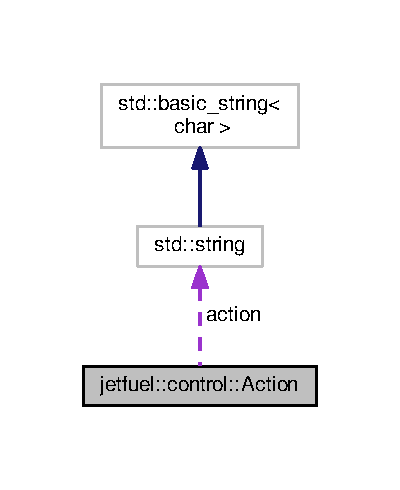
\includegraphics[width=192pt]{structjetfuel_1_1control_1_1Action__coll__graph}
\end{center}
\end{figure}
\subsection*{Public Types}
\begin{DoxyCompactItemize}
\item 
\mbox{\Hypertarget{structjetfuel_1_1control_1_1Action_a619ce738704c0ff88688056437e8743a}\label{structjetfuel_1_1control_1_1Action_a619ce738704c0ff88688056437e8743a}} 
enum {\bfseries Input\+\_\+state} \{ {\bfseries Up}, 
{\bfseries Down}
 \}
\item 
\mbox{\Hypertarget{structjetfuel_1_1control_1_1Action_a52c78bcd5d7251daa99fa97487356a75}\label{structjetfuel_1_1control_1_1Action_a52c78bcd5d7251daa99fa97487356a75}} 
enum {\bfseries Input\+\_\+type} \{ {\bfseries Mouse}, 
{\bfseries Keyboard}, 
{\bfseries Joystick}, 
{\bfseries Touch}
 \}
\end{DoxyCompactItemize}
\subsection*{Public Attributes}
\begin{DoxyCompactItemize}
\item 
\mbox{\Hypertarget{structjetfuel_1_1control_1_1Action_adb7c74c79316332833660dc60906184c}\label{structjetfuel_1_1control_1_1Action_adb7c74c79316332833660dc60906184c}} 
std\+::string {\bfseries action}
\item 
\mbox{\Hypertarget{structjetfuel_1_1control_1_1Action_a20d92b3f8f736097e2688df915602cc8}\label{structjetfuel_1_1control_1_1Action_a20d92b3f8f736097e2688df915602cc8}} 
Input\+\_\+state {\bfseries inputstate}
\item 
\mbox{\Hypertarget{structjetfuel_1_1control_1_1Action_a948114eb27a949423e311103ace134b1}\label{structjetfuel_1_1control_1_1Action_a948114eb27a949423e311103ace134b1}} 
Input\+\_\+type {\bfseries inputtype}
\end{DoxyCompactItemize}


\subsection{Detailed Description}
An interpreted \hyperlink{structjetfuel_1_1control_1_1Action}{Action} produced from an Universal Input System Interpreter(jetfuel\+::control\+::\+U\+I\+S\+\_\+interpreter).

For a code example, refer to the code sample provided with \hyperlink{classjetfuel_1_1control_1_1UIS__interpreter}{jetfuel\+::control\+::\+U\+I\+S\+\_\+interpreter}. 

The documentation for this struct was generated from the following file\+:\begin{DoxyCompactItemize}
\item 
include/jetfuelcontrol/U\+I\+Sinterpreter.\+h\end{DoxyCompactItemize}

\hypertarget{classjetfuel_1_1gui_1_1Button}{}\section{jetfuel\+:\+:gui\+:\+:Button Class Reference}
\label{classjetfuel_1_1gui_1_1Button}\index{jetfuel\+::gui\+::\+Button@{jetfuel\+::gui\+::\+Button}}


{\ttfamily \#include $<$button.\+h$>$}



Inheritance diagram for jetfuel\+:\+:gui\+:\+:Button\+:
\nopagebreak
\begin{figure}[H]
\begin{center}
\leavevmode
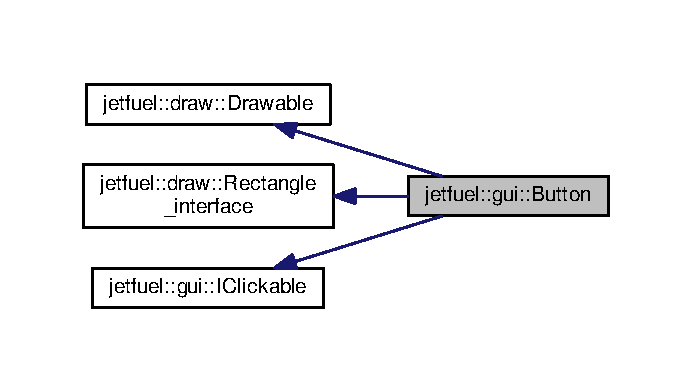
\includegraphics[width=332pt]{classjetfuel_1_1gui_1_1Button__inherit__graph}
\end{center}
\end{figure}


Collaboration diagram for jetfuel\+:\+:gui\+:\+:Button\+:
\nopagebreak
\begin{figure}[H]
\begin{center}
\leavevmode
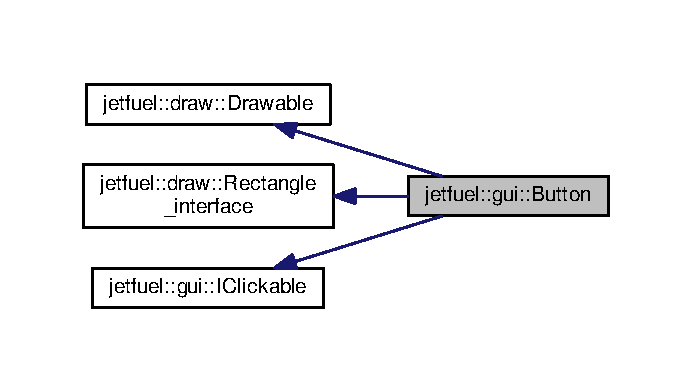
\includegraphics[width=332pt]{classjetfuel_1_1gui_1_1Button__coll__graph}
\end{center}
\end{figure}
\subsection*{Public Member Functions}
\begin{DoxyCompactItemize}
\item 
\hyperlink{classjetfuel_1_1gui_1_1Button_ad9fc0a1426f1fe03563ebac1c4ffcd92}{Button} ()
\begin{DoxyCompactList}\small\item\em Default constructor. \end{DoxyCompactList}\item 
bool \hyperlink{classjetfuel_1_1gui_1_1Button_a2c9b05aeec9661440c2bde16c6bdd791}{Load\+\_\+base\+\_\+button\+\_\+image} (\hyperlink{classjetfuel_1_1draw_1_1Image}{jetfuel\+::draw\+::\+Image} image)
\begin{DoxyCompactList}\small\item\em Loads a base button image to serve as the button\textquotesingle{}s background. \end{DoxyCompactList}\item 
void \hyperlink{classjetfuel_1_1gui_1_1Button_a452110801fca1b3274d574ebc671e8db}{Dynamic\+\_\+load\+\_\+base\+\_\+button\+\_\+image} (\hyperlink{classjetfuel_1_1draw_1_1Image}{jetfuel\+::draw\+::\+Image} image)
\begin{DoxyCompactList}\small\item\em Dynamically load a base button to serve as the button\textquotesingle{}s background. \end{DoxyCompactList}\item 
void \hyperlink{classjetfuel_1_1gui_1_1Button_a1d40cbd21c0c64b0a9c59b598536cce1}{Set\+\_\+button\+\_\+color} (\hyperlink{classjetfuel_1_1draw_1_1Color}{jetfuel\+::draw\+::\+Color} color)
\begin{DoxyCompactList}\small\item\em Sets the button\textquotesingle{}s color overlay to be overlaid over the background\textquotesingle{}s image. \end{DoxyCompactList}\item 
void \hyperlink{classjetfuel_1_1gui_1_1Button_ab2cf5dbf928df48a55118652e003519a}{Set\+\_\+button\+\_\+text\+\_\+characteristics} (\hyperlink{structjetfuel_1_1draw_1_1Text_1_1Text__characteristics}{jetfuel\+::draw\+::\+Text\+::\+Text\+\_\+characteristics} buttontextchars)
\begin{DoxyCompactList}\small\item\em Sets the button\textquotesingle{}s text characteristics when displaying text. \end{DoxyCompactList}\item 
void \hyperlink{classjetfuel_1_1gui_1_1Button_a4b256fdcf0ae28d8fb258b0f89d19536}{Set\+\_\+clicked\+\_\+message} (const std\+::string message, \hyperlink{classjetfuel_1_1core_1_1Message__bus}{jetfuel\+::core\+::\+Message\+\_\+bus} $\ast$bus)
\begin{DoxyCompactList}\small\item\em Sets the message to send to the message bus passed into this function when this button is clicked. \end{DoxyCompactList}\item 
void \hyperlink{classjetfuel_1_1gui_1_1Button_a174b285f6271813e83fe277402ea3b8b}{Set\+\_\+\+U\+I\+S\+\_\+action\+\_\+to\+\_\+watch} (const std\+::string action)
\begin{DoxyCompactList}\small\item\em Sets the Universal Input System(\+U\+I\+S) action to watch for clicks. \end{DoxyCompactList}\item 
void \hyperlink{classjetfuel_1_1gui_1_1Button_ab80239583f2e515370a90771976c5265}{Check\+\_\+for\+\_\+clicks} (\hyperlink{structjetfuel_1_1control_1_1Action}{jetfuel\+::control\+::\+Action} U\+I\+Sinterpreterdata) override
\begin{DoxyCompactList}\small\item\em Checks for clicks. \end{DoxyCompactList}\item 
void \hyperlink{classjetfuel_1_1gui_1_1Button_aa566a1d59623fde8d062c3d02b6fd5f4}{Assign\+\_\+renderer} (S\+D\+L\+\_\+\+Renderer $\ast$renderer) override
\begin{DoxyCompactList}\small\item\em Assigns renderer to this button\textquotesingle{}s Drawables. \end{DoxyCompactList}\item 
bool \hyperlink{classjetfuel_1_1gui_1_1Button_a52c175819af166cda4c000fc2e32fb25}{Has\+\_\+been\+\_\+assigned\+\_\+renderer} ()
\begin{DoxyCompactList}\small\item\em Returns whether this \hyperlink{classjetfuel_1_1gui_1_1Button}{Button} has been assigned a renderer. \end{DoxyCompactList}\item 
\hyperlink{classjetfuel_1_1draw_1_1Vector2d}{jetfuel\+::draw\+::\+Vector2d\+\_\+int} \hyperlink{classjetfuel_1_1gui_1_1Button_aadcceacaabaa40bceb293d1f91231d22}{Get\+\_\+position} () override
\begin{DoxyCompactList}\small\item\em Gets this \hyperlink{classjetfuel_1_1gui_1_1Button}{Button}\textquotesingle{}s position on the screen. \end{DoxyCompactList}\item 
void \hyperlink{classjetfuel_1_1gui_1_1Button_a642d3f1412339c826458b80dce76ef34}{Set\+\_\+position} (\hyperlink{classjetfuel_1_1draw_1_1Vector2d}{jetfuel\+::draw\+::\+Vector2d\+\_\+int} position) override
\begin{DoxyCompactList}\small\item\em Sets this \hyperlink{classjetfuel_1_1gui_1_1Button}{Button}\textquotesingle{}s position on the screen. \end{DoxyCompactList}\item 
\hyperlink{classjetfuel_1_1draw_1_1Rect2d}{jetfuel\+::draw\+::\+Rect2d\+\_\+int} \hyperlink{classjetfuel_1_1gui_1_1Button_a99615af8c169d2274b1593a29fdaf7ca}{Get\+\_\+rect\+\_\+to\+\_\+draw} () override
\begin{DoxyCompactList}\small\item\em Gets this \hyperlink{classjetfuel_1_1gui_1_1Button}{Button}\textquotesingle{}s rectangle that will be drawn on the screen. \end{DoxyCompactList}\item 
void \hyperlink{classjetfuel_1_1gui_1_1Button_a4269075522becce58d220d3aa4bbd6ec}{Force\+\_\+load\+\_\+dynamic\+\_\+image} ()
\begin{DoxyCompactList}\small\item\em Force loads the \hyperlink{classjetfuel_1_1gui_1_1Button}{Button}\textquotesingle{}s dynamic image, if any. \end{DoxyCompactList}\item 
bool \hyperlink{classjetfuel_1_1gui_1_1Button_a1c8ec68b90dc461b1603c47fb8c509c4}{Draw} () override
\begin{DoxyCompactList}\small\item\em Draws this \hyperlink{classjetfuel_1_1gui_1_1Button}{Button} to the screen. \end{DoxyCompactList}\end{DoxyCompactItemize}
\subsection*{Protected Member Functions}
\begin{DoxyCompactItemize}
\item 
bool \hyperlink{classjetfuel_1_1gui_1_1Button_a1572eec073adf699c280ffa784fa7459}{Is\+\_\+ready\+\_\+to\+\_\+draw} () const
\begin{DoxyCompactList}\small\item\em Returns whether this \hyperlink{classjetfuel_1_1gui_1_1Button}{Button}\textquotesingle{}s Drawables are ready to be drawn. \end{DoxyCompactList}\item 
bool \hyperlink{classjetfuel_1_1gui_1_1Button_a548ffd5860aced3206da4c210b5496c9}{Draw\+\_\+button\+\_\+sprite} ()
\begin{DoxyCompactList}\small\item\em Draws this \hyperlink{classjetfuel_1_1gui_1_1Button}{Button}\textquotesingle{}s Sprite object and returns the result. \end{DoxyCompactList}\item 
bool \hyperlink{classjetfuel_1_1gui_1_1Button_ae1e89337652fc30fb7c4997f5b887da3}{Draw\+\_\+button\+\_\+overlay} ()
\begin{DoxyCompactList}\small\item\em Draws this \hyperlink{classjetfuel_1_1gui_1_1Button}{Button}\textquotesingle{}s color overlay object and returns the result. \end{DoxyCompactList}\item 
bool \hyperlink{classjetfuel_1_1gui_1_1Button_ae001860ae9ce670073a4608811e70cfe}{Draw\+\_\+button\+\_\+text} ()
\begin{DoxyCompactList}\small\item\em Draws this \hyperlink{classjetfuel_1_1gui_1_1Button}{Button}\textquotesingle{}s text object and returns the result. \end{DoxyCompactList}\item 
bool \hyperlink{classjetfuel_1_1gui_1_1Button_ac6e616b98179911dd626b018e54b08d7}{Is\+\_\+render\+\_\+ready} () const
\begin{DoxyCompactList}\small\item\em Returns whether the renderer is ready. \end{DoxyCompactList}\end{DoxyCompactItemize}


\subsection{Detailed Description}
A clickable button with a Sprite background displaying an image, a color overlay, and text.

Code Example\+: \hyperlink{classjetfuel_1_1draw_1_1Scene__manager}{jetfuel\+::draw\+::\+Scene\+\_\+manager} scenemanager; \hyperlink{classjetfuel_1_1draw_1_1Scene}{jetfuel\+::draw\+::\+Scene} scene1(1); \hyperlink{classjetfuel_1_1core_1_1Message__bus}{jetfuel\+::core\+::\+Message\+\_\+bus} messagebus; \hyperlink{classjetfuel_1_1gui_1_1Button}{jetfuel\+::gui\+::\+Button} button; \hyperlink{classjetfuel_1_1draw_1_1Image}{jetfuel\+::draw\+::\+Image} buttonimage(\char`\"{}button.\+png\char`\"{}, \&scenemanager); \hyperlink{classjetfuel_1_1control_1_1UIS__manager}{jetfuel\+::control\+::\+U\+I\+S\+\_\+manager} U\+I\+Smanager(\&messagebus, scenemanager.\+Get\+\_\+window\+\_\+id()); \hyperlink{classjetfuel_1_1control_1_1UIS__interpreter}{jetfuel\+::control\+::\+U\+I\+S\+\_\+interpreter} U\+I\+Sinterpreter(\&messagebus); \hyperlink{structjetfuel_1_1draw_1_1Text_1_1Text__characteristics}{jetfuel\+::draw\+::\+Text\+::\+Text\+\_\+characteristics} textchars; \hyperlink{classjetfuel_1_1draw_1_1Font}{jetfuel\+::draw\+::\+Font} font(\char`\"{}default.\+ttf\char`\"{});

if(!scenemanager.Create\+\_\+window(\char`\"{}\+Hello Buttons!\char`\"{}, jetfuel\+::draw\+::\+Vector2d\+\_\+int(0,0), jetfuel\+::draw\+::\+Vector2d\+\_\+int(640,480)))\{ std\+::cout $<$$<$ \char`\"{}\mbox{[}!\mbox{]}\+E\+R\+R\+O\+R with creating sdl window! Error is\+:\char`\"{} $<$$<$ S\+D\+L\+\_\+\+Get\+Error() $<$$<$ \char`\"{}\textbackslash{}n\char`\"{}; \}

if(!scenemanager.Create\+\_\+renderer())\{ std\+::cout $<$$<$ \char`\"{}\mbox{[}!\mbox{]}\+E\+R\+R\+O\+R with creating sdl renderer! Error is\+:\char`\"{} $<$$<$ S\+D\+L\+\_\+\+Get\+Error() $<$$<$ \char`\"{}\textbackslash{}n\char`\"{}; \} scenemanager.\+Switch\+\_\+current\+\_\+scene(\&scene1); scene1.\+Attach\+\_\+drawable(\&button,1);

if(!button.Load\+\_\+base\+\_\+button\+\_\+image(backgroundimage))\{ std\+::cerr $<$$<$ \char`\"{}\mbox{[}!\mbox{]}\+E\+R\+R\+O\+R with loading from image! Error is\+:\char`\"{} $<$$<$ I\+M\+G\+\_\+\+Get\+Error() $<$$<$ \char`\"{}\textbackslash{}n\char`\"{}; \}

button.\+Set\+\_\+position(jetfuel\+::draw\+::\+Vector2d\+\_\+int(0,0));

textchars.\+textstring = \char`\"{}hello\char`\"{}; textchars.\+font = font;

button.\+Set\+\_\+button\+\_\+text\+\_\+characteristics(textchars);

scenemanager.\+Draw\+\_\+current\+\_\+scene(); 

\subsection{Constructor \& Destructor Documentation}
\mbox{\Hypertarget{classjetfuel_1_1gui_1_1Button_ad9fc0a1426f1fe03563ebac1c4ffcd92}\label{classjetfuel_1_1gui_1_1Button_ad9fc0a1426f1fe03563ebac1c4ffcd92}} 
\index{jetfuel\+::gui\+::\+Button@{jetfuel\+::gui\+::\+Button}!Button@{Button}}
\index{Button@{Button}!jetfuel\+::gui\+::\+Button@{jetfuel\+::gui\+::\+Button}}
\subsubsection{\texorpdfstring{Button()}{Button()}}
{\footnotesize\ttfamily jetfuel\+::gui\+::\+Button\+::\+Button (\begin{DoxyParamCaption}{ }\end{DoxyParamCaption})\hspace{0.3cm}{\ttfamily [inline]}}



Default constructor. 

Constructs an empty \hyperlink{classjetfuel_1_1gui_1_1Button}{Button} object. 

\subsection{Member Function Documentation}
\mbox{\Hypertarget{classjetfuel_1_1gui_1_1Button_aa566a1d59623fde8d062c3d02b6fd5f4}\label{classjetfuel_1_1gui_1_1Button_aa566a1d59623fde8d062c3d02b6fd5f4}} 
\index{jetfuel\+::gui\+::\+Button@{jetfuel\+::gui\+::\+Button}!Assign\+\_\+renderer@{Assign\+\_\+renderer}}
\index{Assign\+\_\+renderer@{Assign\+\_\+renderer}!jetfuel\+::gui\+::\+Button@{jetfuel\+::gui\+::\+Button}}
\subsubsection{\texorpdfstring{Assign\+\_\+renderer()}{Assign\_renderer()}}
{\footnotesize\ttfamily void jetfuel\+::gui\+::\+Button\+::\+Assign\+\_\+renderer (\begin{DoxyParamCaption}\item[{S\+D\+L\+\_\+\+Renderer $\ast$}]{renderer }\end{DoxyParamCaption})\hspace{0.3cm}{\ttfamily [override]}, {\ttfamily [virtual]}}



Assigns renderer to this button\textquotesingle{}s Drawables. 

Assigns renderer to this button\textquotesingle{}s Drawables, including the \hyperlink{classjetfuel_1_1gui_1_1Button}{Button}\textquotesingle{}s text, rectangle, and sprite Drawables.


\begin{DoxyParams}{Parameters}
{\em S\+D\+L\+\_\+\+Renderer} & $\ast$renderer \\
\hline
\end{DoxyParams}


Reimplemented from \hyperlink{classjetfuel_1_1draw_1_1Drawable_a0d7257f197d6ffcdd89c3a99c93d1400}{jetfuel\+::draw\+::\+Drawable}.

\mbox{\Hypertarget{classjetfuel_1_1gui_1_1Button_ab80239583f2e515370a90771976c5265}\label{classjetfuel_1_1gui_1_1Button_ab80239583f2e515370a90771976c5265}} 
\index{jetfuel\+::gui\+::\+Button@{jetfuel\+::gui\+::\+Button}!Check\+\_\+for\+\_\+clicks@{Check\+\_\+for\+\_\+clicks}}
\index{Check\+\_\+for\+\_\+clicks@{Check\+\_\+for\+\_\+clicks}!jetfuel\+::gui\+::\+Button@{jetfuel\+::gui\+::\+Button}}
\subsubsection{\texorpdfstring{Check\+\_\+for\+\_\+clicks()}{Check\_for\_clicks()}}
{\footnotesize\ttfamily void jetfuel\+::gui\+::\+Button\+::\+Check\+\_\+for\+\_\+clicks (\begin{DoxyParamCaption}\item[{\hyperlink{structjetfuel_1_1control_1_1Action}{jetfuel\+::control\+::\+Action}}]{U\+I\+Sinterpreterdata }\end{DoxyParamCaption})\hspace{0.3cm}{\ttfamily [override]}, {\ttfamily [virtual]}}



Checks for clicks. 

Checks for clicks. If click is detected, the specified message specified in the Set\+\_\+clicked\+\_\+message function will be sent to the specified message bus.


\begin{DoxyParams}{Parameters}
{\em \hyperlink{structjetfuel_1_1control_1_1Action}{jetfuel\+::control\+::\+Action}} & U\+I\+Sinterpreterdata \\
\hline
\end{DoxyParams}


Implements \hyperlink{classjetfuel_1_1gui_1_1IClickable_aea45de37bd3beb7eb7e2e3056e4e37b3}{jetfuel\+::gui\+::\+I\+Clickable}.

\mbox{\Hypertarget{classjetfuel_1_1gui_1_1Button_a1c8ec68b90dc461b1603c47fb8c509c4}\label{classjetfuel_1_1gui_1_1Button_a1c8ec68b90dc461b1603c47fb8c509c4}} 
\index{jetfuel\+::gui\+::\+Button@{jetfuel\+::gui\+::\+Button}!Draw@{Draw}}
\index{Draw@{Draw}!jetfuel\+::gui\+::\+Button@{jetfuel\+::gui\+::\+Button}}
\subsubsection{\texorpdfstring{Draw()}{Draw()}}
{\footnotesize\ttfamily bool jetfuel\+::gui\+::\+Button\+::\+Draw (\begin{DoxyParamCaption}{ }\end{DoxyParamCaption})\hspace{0.3cm}{\ttfamily [override]}, {\ttfamily [virtual]}}



Draws this \hyperlink{classjetfuel_1_1gui_1_1Button}{Button} to the screen. 

Draws this \hyperlink{classjetfuel_1_1gui_1_1Button}{Button} to the screen. This W\+I\+LL fail if either the renderer has not been assigned(which happens when you attach a \hyperlink{classjetfuel_1_1gui_1_1Button}{Button} to a \hyperlink{classjetfuel_1_1draw_1_1Scene}{jetfuel\+::draw\+::\+Scene}), or the image has not been loaded. If it does, this function will return a boolean of false. Otherwise, it will return a boolean of true. 

Implements \hyperlink{classjetfuel_1_1draw_1_1Drawable_a1a072070322965ce9411ee6e7c311c56}{jetfuel\+::draw\+::\+Drawable}.

\mbox{\Hypertarget{classjetfuel_1_1gui_1_1Button_ae1e89337652fc30fb7c4997f5b887da3}\label{classjetfuel_1_1gui_1_1Button_ae1e89337652fc30fb7c4997f5b887da3}} 
\index{jetfuel\+::gui\+::\+Button@{jetfuel\+::gui\+::\+Button}!Draw\+\_\+button\+\_\+overlay@{Draw\+\_\+button\+\_\+overlay}}
\index{Draw\+\_\+button\+\_\+overlay@{Draw\+\_\+button\+\_\+overlay}!jetfuel\+::gui\+::\+Button@{jetfuel\+::gui\+::\+Button}}
\subsubsection{\texorpdfstring{Draw\+\_\+button\+\_\+overlay()}{Draw\_button\_overlay()}}
{\footnotesize\ttfamily bool jetfuel\+::gui\+::\+Button\+::\+Draw\+\_\+button\+\_\+overlay (\begin{DoxyParamCaption}{ }\end{DoxyParamCaption})\hspace{0.3cm}{\ttfamily [inline]}, {\ttfamily [protected]}}



Draws this \hyperlink{classjetfuel_1_1gui_1_1Button}{Button}\textquotesingle{}s color overlay object and returns the result. 

Draws this \hyperlink{classjetfuel_1_1gui_1_1Button}{Button}\textquotesingle{}s color overlay object and returns the result. \mbox{\Hypertarget{classjetfuel_1_1gui_1_1Button_a548ffd5860aced3206da4c210b5496c9}\label{classjetfuel_1_1gui_1_1Button_a548ffd5860aced3206da4c210b5496c9}} 
\index{jetfuel\+::gui\+::\+Button@{jetfuel\+::gui\+::\+Button}!Draw\+\_\+button\+\_\+sprite@{Draw\+\_\+button\+\_\+sprite}}
\index{Draw\+\_\+button\+\_\+sprite@{Draw\+\_\+button\+\_\+sprite}!jetfuel\+::gui\+::\+Button@{jetfuel\+::gui\+::\+Button}}
\subsubsection{\texorpdfstring{Draw\+\_\+button\+\_\+sprite()}{Draw\_button\_sprite()}}
{\footnotesize\ttfamily bool jetfuel\+::gui\+::\+Button\+::\+Draw\+\_\+button\+\_\+sprite (\begin{DoxyParamCaption}{ }\end{DoxyParamCaption})\hspace{0.3cm}{\ttfamily [inline]}, {\ttfamily [protected]}}



Draws this \hyperlink{classjetfuel_1_1gui_1_1Button}{Button}\textquotesingle{}s Sprite object and returns the result. 

Draws this \hyperlink{classjetfuel_1_1gui_1_1Button}{Button}\textquotesingle{}s Sprite object and returns the result. \mbox{\Hypertarget{classjetfuel_1_1gui_1_1Button_ae001860ae9ce670073a4608811e70cfe}\label{classjetfuel_1_1gui_1_1Button_ae001860ae9ce670073a4608811e70cfe}} 
\index{jetfuel\+::gui\+::\+Button@{jetfuel\+::gui\+::\+Button}!Draw\+\_\+button\+\_\+text@{Draw\+\_\+button\+\_\+text}}
\index{Draw\+\_\+button\+\_\+text@{Draw\+\_\+button\+\_\+text}!jetfuel\+::gui\+::\+Button@{jetfuel\+::gui\+::\+Button}}
\subsubsection{\texorpdfstring{Draw\+\_\+button\+\_\+text()}{Draw\_button\_text()}}
{\footnotesize\ttfamily bool jetfuel\+::gui\+::\+Button\+::\+Draw\+\_\+button\+\_\+text (\begin{DoxyParamCaption}{ }\end{DoxyParamCaption})\hspace{0.3cm}{\ttfamily [inline]}, {\ttfamily [protected]}}



Draws this \hyperlink{classjetfuel_1_1gui_1_1Button}{Button}\textquotesingle{}s text object and returns the result. 

Draws this \hyperlink{classjetfuel_1_1gui_1_1Button}{Button}\textquotesingle{}s text object and returns the result. \mbox{\Hypertarget{classjetfuel_1_1gui_1_1Button_a452110801fca1b3274d574ebc671e8db}\label{classjetfuel_1_1gui_1_1Button_a452110801fca1b3274d574ebc671e8db}} 
\index{jetfuel\+::gui\+::\+Button@{jetfuel\+::gui\+::\+Button}!Dynamic\+\_\+load\+\_\+base\+\_\+button\+\_\+image@{Dynamic\+\_\+load\+\_\+base\+\_\+button\+\_\+image}}
\index{Dynamic\+\_\+load\+\_\+base\+\_\+button\+\_\+image@{Dynamic\+\_\+load\+\_\+base\+\_\+button\+\_\+image}!jetfuel\+::gui\+::\+Button@{jetfuel\+::gui\+::\+Button}}
\subsubsection{\texorpdfstring{Dynamic\+\_\+load\+\_\+base\+\_\+button\+\_\+image()}{Dynamic\_load\_base\_button\_image()}}
{\footnotesize\ttfamily void jetfuel\+::gui\+::\+Button\+::\+Dynamic\+\_\+load\+\_\+base\+\_\+button\+\_\+image (\begin{DoxyParamCaption}\item[{\hyperlink{classjetfuel_1_1draw_1_1Image}{jetfuel\+::draw\+::\+Image}}]{image }\end{DoxyParamCaption})\hspace{0.3cm}{\ttfamily [inline]}}



Dynamically load a base button to serve as the button\textquotesingle{}s background. 

Dynamically load a base button to serve as the button\textquotesingle{}s background placed underneath the button\textquotesingle{}s text and color overlay.


\begin{DoxyParams}{Parameters}
{\em \hyperlink{classjetfuel_1_1draw_1_1Image}{jetfuel\+::draw\+::\+Image}} & image \\
\hline
\end{DoxyParams}
\mbox{\Hypertarget{classjetfuel_1_1gui_1_1Button_a4269075522becce58d220d3aa4bbd6ec}\label{classjetfuel_1_1gui_1_1Button_a4269075522becce58d220d3aa4bbd6ec}} 
\index{jetfuel\+::gui\+::\+Button@{jetfuel\+::gui\+::\+Button}!Force\+\_\+load\+\_\+dynamic\+\_\+image@{Force\+\_\+load\+\_\+dynamic\+\_\+image}}
\index{Force\+\_\+load\+\_\+dynamic\+\_\+image@{Force\+\_\+load\+\_\+dynamic\+\_\+image}!jetfuel\+::gui\+::\+Button@{jetfuel\+::gui\+::\+Button}}
\subsubsection{\texorpdfstring{Force\+\_\+load\+\_\+dynamic\+\_\+image()}{Force\_load\_dynamic\_image()}}
{\footnotesize\ttfamily void jetfuel\+::gui\+::\+Button\+::\+Force\+\_\+load\+\_\+dynamic\+\_\+image (\begin{DoxyParamCaption}{ }\end{DoxyParamCaption})\hspace{0.3cm}{\ttfamily [inline]}}



Force loads the \hyperlink{classjetfuel_1_1gui_1_1Button}{Button}\textquotesingle{}s dynamic image, if any. 

Force loads the \hyperlink{classjetfuel_1_1gui_1_1Button}{Button}\textquotesingle{}s dynamic image, if any. It will re-\/load the image also when the Draw function is called even if you call this function. This function is mainly to find out the height and width of the sprite\textquotesingle{}s image and not much else. \mbox{\Hypertarget{classjetfuel_1_1gui_1_1Button_aadcceacaabaa40bceb293d1f91231d22}\label{classjetfuel_1_1gui_1_1Button_aadcceacaabaa40bceb293d1f91231d22}} 
\index{jetfuel\+::gui\+::\+Button@{jetfuel\+::gui\+::\+Button}!Get\+\_\+position@{Get\+\_\+position}}
\index{Get\+\_\+position@{Get\+\_\+position}!jetfuel\+::gui\+::\+Button@{jetfuel\+::gui\+::\+Button}}
\subsubsection{\texorpdfstring{Get\+\_\+position()}{Get\_position()}}
{\footnotesize\ttfamily \hyperlink{classjetfuel_1_1draw_1_1Vector2d}{jetfuel\+::draw\+::\+Vector2d\+\_\+int} jetfuel\+::gui\+::\+Button\+::\+Get\+\_\+position (\begin{DoxyParamCaption}{ }\end{DoxyParamCaption})\hspace{0.3cm}{\ttfamily [inline]}, {\ttfamily [override]}, {\ttfamily [virtual]}}



Gets this \hyperlink{classjetfuel_1_1gui_1_1Button}{Button}\textquotesingle{}s position on the screen. 

Gets this \hyperlink{classjetfuel_1_1gui_1_1Button}{Button}\textquotesingle{}s position on the screen. 

Reimplemented from \hyperlink{classjetfuel_1_1draw_1_1Drawable_ae7ebd30d66db2c8a5d5371cbcf0023fc}{jetfuel\+::draw\+::\+Drawable}.

\mbox{\Hypertarget{classjetfuel_1_1gui_1_1Button_a99615af8c169d2274b1593a29fdaf7ca}\label{classjetfuel_1_1gui_1_1Button_a99615af8c169d2274b1593a29fdaf7ca}} 
\index{jetfuel\+::gui\+::\+Button@{jetfuel\+::gui\+::\+Button}!Get\+\_\+rect\+\_\+to\+\_\+draw@{Get\+\_\+rect\+\_\+to\+\_\+draw}}
\index{Get\+\_\+rect\+\_\+to\+\_\+draw@{Get\+\_\+rect\+\_\+to\+\_\+draw}!jetfuel\+::gui\+::\+Button@{jetfuel\+::gui\+::\+Button}}
\subsubsection{\texorpdfstring{Get\+\_\+rect\+\_\+to\+\_\+draw()}{Get\_rect\_to\_draw()}}
{\footnotesize\ttfamily \hyperlink{classjetfuel_1_1draw_1_1Rect2d}{jetfuel\+::draw\+::\+Rect2d\+\_\+int} jetfuel\+::gui\+::\+Button\+::\+Get\+\_\+rect\+\_\+to\+\_\+draw (\begin{DoxyParamCaption}{ }\end{DoxyParamCaption})\hspace{0.3cm}{\ttfamily [inline]}, {\ttfamily [override]}, {\ttfamily [virtual]}}



Gets this \hyperlink{classjetfuel_1_1gui_1_1Button}{Button}\textquotesingle{}s rectangle that will be drawn on the screen. 

Gets this \hyperlink{classjetfuel_1_1gui_1_1Button}{Button}\textquotesingle{}s rectangle that will be drawn on the Draw function being called. 

Implements \hyperlink{classjetfuel_1_1draw_1_1Rectangle__interface_a03fd3b6842ab7b3065379caec407296f}{jetfuel\+::draw\+::\+Rectangle\+\_\+interface}.

\mbox{\Hypertarget{classjetfuel_1_1gui_1_1Button_a52c175819af166cda4c000fc2e32fb25}\label{classjetfuel_1_1gui_1_1Button_a52c175819af166cda4c000fc2e32fb25}} 
\index{jetfuel\+::gui\+::\+Button@{jetfuel\+::gui\+::\+Button}!Has\+\_\+been\+\_\+assigned\+\_\+renderer@{Has\+\_\+been\+\_\+assigned\+\_\+renderer}}
\index{Has\+\_\+been\+\_\+assigned\+\_\+renderer@{Has\+\_\+been\+\_\+assigned\+\_\+renderer}!jetfuel\+::gui\+::\+Button@{jetfuel\+::gui\+::\+Button}}
\subsubsection{\texorpdfstring{Has\+\_\+been\+\_\+assigned\+\_\+renderer()}{Has\_been\_assigned\_renderer()}}
{\footnotesize\ttfamily bool jetfuel\+::gui\+::\+Button\+::\+Has\+\_\+been\+\_\+assigned\+\_\+renderer (\begin{DoxyParamCaption}{ }\end{DoxyParamCaption})\hspace{0.3cm}{\ttfamily [inline]}}



Returns whether this \hyperlink{classjetfuel_1_1gui_1_1Button}{Button} has been assigned a renderer. 

Returns whether this \hyperlink{classjetfuel_1_1gui_1_1Button}{Button} has been assigned a renderer. \mbox{\Hypertarget{classjetfuel_1_1gui_1_1Button_a1572eec073adf699c280ffa784fa7459}\label{classjetfuel_1_1gui_1_1Button_a1572eec073adf699c280ffa784fa7459}} 
\index{jetfuel\+::gui\+::\+Button@{jetfuel\+::gui\+::\+Button}!Is\+\_\+ready\+\_\+to\+\_\+draw@{Is\+\_\+ready\+\_\+to\+\_\+draw}}
\index{Is\+\_\+ready\+\_\+to\+\_\+draw@{Is\+\_\+ready\+\_\+to\+\_\+draw}!jetfuel\+::gui\+::\+Button@{jetfuel\+::gui\+::\+Button}}
\subsubsection{\texorpdfstring{Is\+\_\+ready\+\_\+to\+\_\+draw()}{Is\_ready\_to\_draw()}}
{\footnotesize\ttfamily bool jetfuel\+::gui\+::\+Button\+::\+Is\+\_\+ready\+\_\+to\+\_\+draw (\begin{DoxyParamCaption}{ }\end{DoxyParamCaption}) const\hspace{0.3cm}{\ttfamily [inline]}, {\ttfamily [protected]}}



Returns whether this \hyperlink{classjetfuel_1_1gui_1_1Button}{Button}\textquotesingle{}s Drawables are ready to be drawn. 

Returns whether this \hyperlink{classjetfuel_1_1gui_1_1Button}{Button}\textquotesingle{}s Drawables are ready to be drawn. \mbox{\Hypertarget{classjetfuel_1_1gui_1_1Button_ac6e616b98179911dd626b018e54b08d7}\label{classjetfuel_1_1gui_1_1Button_ac6e616b98179911dd626b018e54b08d7}} 
\index{jetfuel\+::gui\+::\+Button@{jetfuel\+::gui\+::\+Button}!Is\+\_\+render\+\_\+ready@{Is\+\_\+render\+\_\+ready}}
\index{Is\+\_\+render\+\_\+ready@{Is\+\_\+render\+\_\+ready}!jetfuel\+::gui\+::\+Button@{jetfuel\+::gui\+::\+Button}}
\subsubsection{\texorpdfstring{Is\+\_\+render\+\_\+ready()}{Is\_render\_ready()}}
{\footnotesize\ttfamily bool jetfuel\+::gui\+::\+Button\+::\+Is\+\_\+render\+\_\+ready (\begin{DoxyParamCaption}{ }\end{DoxyParamCaption}) const\hspace{0.3cm}{\ttfamily [inline]}, {\ttfamily [protected]}}



Returns whether the renderer is ready. 

Returns whether the renderer is ready. \mbox{\Hypertarget{classjetfuel_1_1gui_1_1Button_a2c9b05aeec9661440c2bde16c6bdd791}\label{classjetfuel_1_1gui_1_1Button_a2c9b05aeec9661440c2bde16c6bdd791}} 
\index{jetfuel\+::gui\+::\+Button@{jetfuel\+::gui\+::\+Button}!Load\+\_\+base\+\_\+button\+\_\+image@{Load\+\_\+base\+\_\+button\+\_\+image}}
\index{Load\+\_\+base\+\_\+button\+\_\+image@{Load\+\_\+base\+\_\+button\+\_\+image}!jetfuel\+::gui\+::\+Button@{jetfuel\+::gui\+::\+Button}}
\subsubsection{\texorpdfstring{Load\+\_\+base\+\_\+button\+\_\+image()}{Load\_base\_button\_image()}}
{\footnotesize\ttfamily bool jetfuel\+::gui\+::\+Button\+::\+Load\+\_\+base\+\_\+button\+\_\+image (\begin{DoxyParamCaption}\item[{\hyperlink{classjetfuel_1_1draw_1_1Image}{jetfuel\+::draw\+::\+Image}}]{image }\end{DoxyParamCaption})\hspace{0.3cm}{\ttfamily [inline]}}



Loads a base button image to serve as the button\textquotesingle{}s background. 

Loads a base button image to serve as the button\textquotesingle{}s background placed underneath the button\textquotesingle{}s text and color overlay.


\begin{DoxyParams}{Parameters}
{\em \hyperlink{classjetfuel_1_1draw_1_1Image}{jetfuel\+::draw\+::\+Image}} & image \\
\hline
\end{DoxyParams}
\mbox{\Hypertarget{classjetfuel_1_1gui_1_1Button_a1d40cbd21c0c64b0a9c59b598536cce1}\label{classjetfuel_1_1gui_1_1Button_a1d40cbd21c0c64b0a9c59b598536cce1}} 
\index{jetfuel\+::gui\+::\+Button@{jetfuel\+::gui\+::\+Button}!Set\+\_\+button\+\_\+color@{Set\+\_\+button\+\_\+color}}
\index{Set\+\_\+button\+\_\+color@{Set\+\_\+button\+\_\+color}!jetfuel\+::gui\+::\+Button@{jetfuel\+::gui\+::\+Button}}
\subsubsection{\texorpdfstring{Set\+\_\+button\+\_\+color()}{Set\_button\_color()}}
{\footnotesize\ttfamily void jetfuel\+::gui\+::\+Button\+::\+Set\+\_\+button\+\_\+color (\begin{DoxyParamCaption}\item[{\hyperlink{classjetfuel_1_1draw_1_1Color}{jetfuel\+::draw\+::\+Color}}]{color }\end{DoxyParamCaption})}



Sets the button\textquotesingle{}s color overlay to be overlaid over the background\textquotesingle{}s image. 

Sets the button\textquotesingle{}s color overlay to be overlaid over the background\textquotesingle{}s image.


\begin{DoxyParams}{Parameters}
{\em \hyperlink{classjetfuel_1_1draw_1_1Color}{jetfuel\+::draw\+::\+Color}} & color \\
\hline
\end{DoxyParams}
\mbox{\Hypertarget{classjetfuel_1_1gui_1_1Button_ab2cf5dbf928df48a55118652e003519a}\label{classjetfuel_1_1gui_1_1Button_ab2cf5dbf928df48a55118652e003519a}} 
\index{jetfuel\+::gui\+::\+Button@{jetfuel\+::gui\+::\+Button}!Set\+\_\+button\+\_\+text\+\_\+characteristics@{Set\+\_\+button\+\_\+text\+\_\+characteristics}}
\index{Set\+\_\+button\+\_\+text\+\_\+characteristics@{Set\+\_\+button\+\_\+text\+\_\+characteristics}!jetfuel\+::gui\+::\+Button@{jetfuel\+::gui\+::\+Button}}
\subsubsection{\texorpdfstring{Set\+\_\+button\+\_\+text\+\_\+characteristics()}{Set\_button\_text\_characteristics()}}
{\footnotesize\ttfamily void jetfuel\+::gui\+::\+Button\+::\+Set\+\_\+button\+\_\+text\+\_\+characteristics (\begin{DoxyParamCaption}\item[{\hyperlink{structjetfuel_1_1draw_1_1Text_1_1Text__characteristics}{jetfuel\+::draw\+::\+Text\+::\+Text\+\_\+characteristics}}]{buttontextchars }\end{DoxyParamCaption})\hspace{0.3cm}{\ttfamily [inline]}}



Sets the button\textquotesingle{}s text characteristics when displaying text. 

Sets the button\textquotesingle{}s text characteristics when displaying text. Text characteristics are text options like Font, font hinting, text size, and text color that can easily be set via this one function!


\begin{DoxyParams}{Parameters}
{\em \hyperlink{structjetfuel_1_1draw_1_1Text_1_1Text__characteristics}{jetfuel\+::draw\+::\+Text\+::\+Text\+\_\+characteristics}} & \\
\hline
\end{DoxyParams}
\mbox{\Hypertarget{classjetfuel_1_1gui_1_1Button_a4b256fdcf0ae28d8fb258b0f89d19536}\label{classjetfuel_1_1gui_1_1Button_a4b256fdcf0ae28d8fb258b0f89d19536}} 
\index{jetfuel\+::gui\+::\+Button@{jetfuel\+::gui\+::\+Button}!Set\+\_\+clicked\+\_\+message@{Set\+\_\+clicked\+\_\+message}}
\index{Set\+\_\+clicked\+\_\+message@{Set\+\_\+clicked\+\_\+message}!jetfuel\+::gui\+::\+Button@{jetfuel\+::gui\+::\+Button}}
\subsubsection{\texorpdfstring{Set\+\_\+clicked\+\_\+message()}{Set\_clicked\_message()}}
{\footnotesize\ttfamily void jetfuel\+::gui\+::\+Button\+::\+Set\+\_\+clicked\+\_\+message (\begin{DoxyParamCaption}\item[{const std\+::string}]{message,  }\item[{\hyperlink{classjetfuel_1_1core_1_1Message__bus}{jetfuel\+::core\+::\+Message\+\_\+bus} $\ast$}]{bus }\end{DoxyParamCaption})\hspace{0.3cm}{\ttfamily [inline]}}



Sets the message to send to the message bus passed into this function when this button is clicked. 

Sets the message to send to the message bus passed into this function when this button is clicked.


\begin{DoxyParams}{Parameters}
{\em std\+::string} & message \\
\hline
{\em \hyperlink{classjetfuel_1_1core_1_1Message__bus}{jetfuel\+::core\+::\+Message\+\_\+bus}} & $\ast$bus \\
\hline
\end{DoxyParams}
\mbox{\Hypertarget{classjetfuel_1_1gui_1_1Button_a642d3f1412339c826458b80dce76ef34}\label{classjetfuel_1_1gui_1_1Button_a642d3f1412339c826458b80dce76ef34}} 
\index{jetfuel\+::gui\+::\+Button@{jetfuel\+::gui\+::\+Button}!Set\+\_\+position@{Set\+\_\+position}}
\index{Set\+\_\+position@{Set\+\_\+position}!jetfuel\+::gui\+::\+Button@{jetfuel\+::gui\+::\+Button}}
\subsubsection{\texorpdfstring{Set\+\_\+position()}{Set\_position()}}
{\footnotesize\ttfamily void jetfuel\+::gui\+::\+Button\+::\+Set\+\_\+position (\begin{DoxyParamCaption}\item[{\hyperlink{classjetfuel_1_1draw_1_1Vector2d}{jetfuel\+::draw\+::\+Vector2d\+\_\+int}}]{position }\end{DoxyParamCaption})\hspace{0.3cm}{\ttfamily [inline]}, {\ttfamily [override]}, {\ttfamily [virtual]}}



Sets this \hyperlink{classjetfuel_1_1gui_1_1Button}{Button}\textquotesingle{}s position on the screen. 

Sets this \hyperlink{classjetfuel_1_1gui_1_1Button}{Button}\textquotesingle{}s position on the screen.


\begin{DoxyParams}{Parameters}
{\em jetfuel\+::draw\+::\+Vector2d\+\_\+int} & position \\
\hline
\end{DoxyParams}


Reimplemented from \hyperlink{classjetfuel_1_1draw_1_1Drawable_afdd035afe40c706459a6c9df813bcce6}{jetfuel\+::draw\+::\+Drawable}.

\mbox{\Hypertarget{classjetfuel_1_1gui_1_1Button_a174b285f6271813e83fe277402ea3b8b}\label{classjetfuel_1_1gui_1_1Button_a174b285f6271813e83fe277402ea3b8b}} 
\index{jetfuel\+::gui\+::\+Button@{jetfuel\+::gui\+::\+Button}!Set\+\_\+\+U\+I\+S\+\_\+action\+\_\+to\+\_\+watch@{Set\+\_\+\+U\+I\+S\+\_\+action\+\_\+to\+\_\+watch}}
\index{Set\+\_\+\+U\+I\+S\+\_\+action\+\_\+to\+\_\+watch@{Set\+\_\+\+U\+I\+S\+\_\+action\+\_\+to\+\_\+watch}!jetfuel\+::gui\+::\+Button@{jetfuel\+::gui\+::\+Button}}
\subsubsection{\texorpdfstring{Set\+\_\+\+U\+I\+S\+\_\+action\+\_\+to\+\_\+watch()}{Set\_UIS\_action\_to\_watch()}}
{\footnotesize\ttfamily void jetfuel\+::gui\+::\+Button\+::\+Set\+\_\+\+U\+I\+S\+\_\+action\+\_\+to\+\_\+watch (\begin{DoxyParamCaption}\item[{const std\+::string}]{action }\end{DoxyParamCaption})\hspace{0.3cm}{\ttfamily [inline]}}



Sets the Universal Input System(\+U\+I\+S) action to watch for clicks. 

Sets the Universal Input System(\+U\+I\+S) action to watch for clicks.


\begin{DoxyParams}{Parameters}
{\em std\+::string} & action \\
\hline
\end{DoxyParams}


The documentation for this class was generated from the following file\+:\begin{DoxyCompactItemize}
\item 
include/jetfuelgui/button.\+h\end{DoxyCompactItemize}

\hypertarget{structjetfuel_1_1gui_1_1Menu_1_1Button__characteristics}{}\section{jetfuel\+:\+:gui\+:\+:Menu\+:\+:Button\+\_\+characteristics Struct Reference}
\label{structjetfuel_1_1gui_1_1Menu_1_1Button__characteristics}\index{jetfuel\+::gui\+::\+Menu\+::\+Button\+\_\+characteristics@{jetfuel\+::gui\+::\+Menu\+::\+Button\+\_\+characteristics}}


{\ttfamily \#include $<$menu.\+h$>$}



Collaboration diagram for jetfuel\+:\+:gui\+:\+:Menu\+:\+:Button\+\_\+characteristics\+:
\nopagebreak
\begin{figure}[H]
\begin{center}
\leavevmode
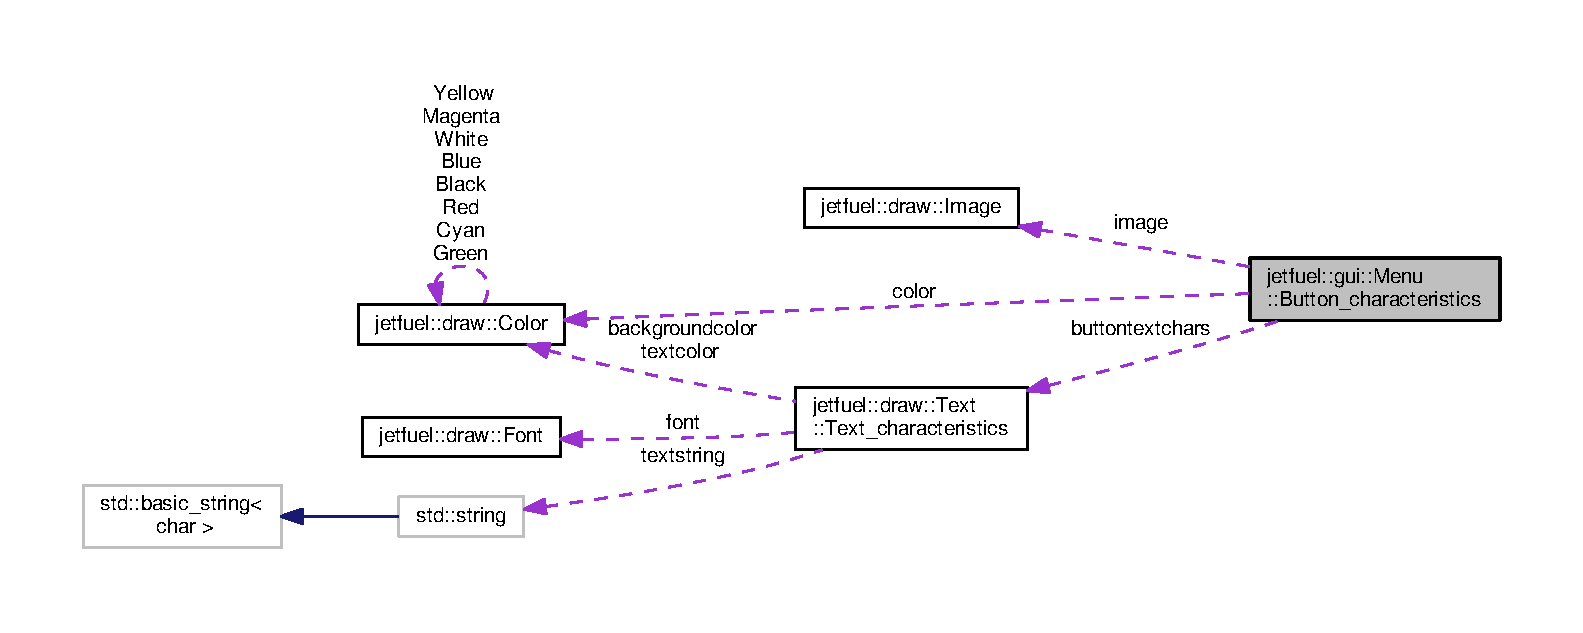
\includegraphics[width=350pt]{structjetfuel_1_1gui_1_1Menu_1_1Button__characteristics__coll__graph}
\end{center}
\end{figure}
\subsection*{Public Attributes}
\begin{DoxyCompactItemize}
\item 
\mbox{\Hypertarget{structjetfuel_1_1gui_1_1Menu_1_1Button__characteristics_ac808e56f02360af082de0acedaa95328}\label{structjetfuel_1_1gui_1_1Menu_1_1Button__characteristics_ac808e56f02360af082de0acedaa95328}} 
\hyperlink{classjetfuel_1_1draw_1_1Image}{jetfuel\+::draw\+::\+Image} {\bfseries image}
\item 
\mbox{\Hypertarget{structjetfuel_1_1gui_1_1Menu_1_1Button__characteristics_a51bce0c5c61b39fb45b6f2267ab9fc17}\label{structjetfuel_1_1gui_1_1Menu_1_1Button__characteristics_a51bce0c5c61b39fb45b6f2267ab9fc17}} 
\hyperlink{classjetfuel_1_1draw_1_1Color}{jetfuel\+::draw\+::\+Color} {\bfseries color}
\item 
\mbox{\Hypertarget{structjetfuel_1_1gui_1_1Menu_1_1Button__characteristics_a19d5d256fb348fd17efe64d23f9d7023}\label{structjetfuel_1_1gui_1_1Menu_1_1Button__characteristics_a19d5d256fb348fd17efe64d23f9d7023}} 
\hyperlink{structjetfuel_1_1draw_1_1Text_1_1Text__characteristics}{jetfuel\+::draw\+::\+Text\+::\+Text\+\_\+characteristics} {\bfseries buttontextchars}
\end{DoxyCompactItemize}


\subsection{Detailed Description}
A simple struct with the characteristics of a \hyperlink{classjetfuel_1_1gui_1_1Button}{jetfuel\+::gui\+::\+Button}. 

The documentation for this struct was generated from the following file\+:\begin{DoxyCompactItemize}
\item 
include/jetfuelgui/menu.\+h\end{DoxyCompactItemize}

\hypertarget{classjetfuel_1_1gui_1_1Check__box}{}\section{jetfuel\+:\+:gui\+:\+:Check\+\_\+box Class Reference}
\label{classjetfuel_1_1gui_1_1Check__box}\index{jetfuel\+::gui\+::\+Check\+\_\+box@{jetfuel\+::gui\+::\+Check\+\_\+box}}


{\ttfamily \#include $<$checkbox.\+h$>$}



Inheritance diagram for jetfuel\+:\+:gui\+:\+:Check\+\_\+box\+:\nopagebreak
\begin{figure}[H]
\begin{center}
\leavevmode
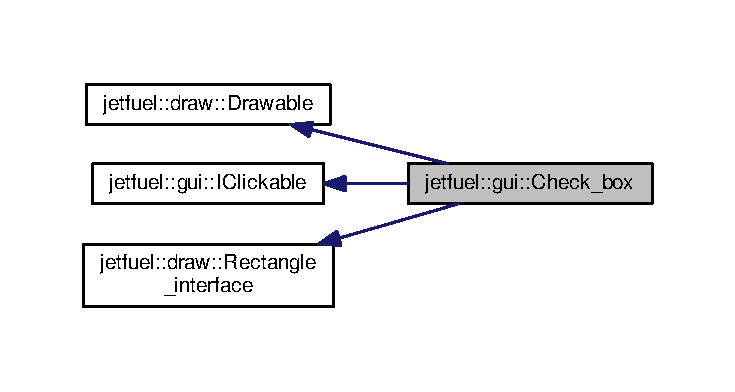
\includegraphics[width=350pt]{classjetfuel_1_1gui_1_1Check__box__inherit__graph}
\end{center}
\end{figure}


Collaboration diagram for jetfuel\+:\+:gui\+:\+:Check\+\_\+box\+:\nopagebreak
\begin{figure}[H]
\begin{center}
\leavevmode
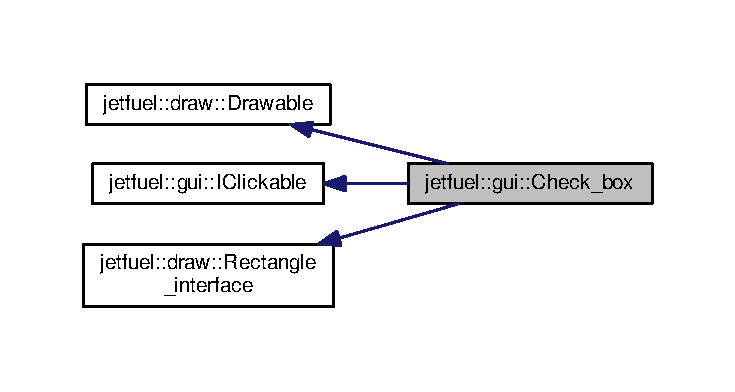
\includegraphics[width=350pt]{classjetfuel_1_1gui_1_1Check__box__coll__graph}
\end{center}
\end{figure}
\subsection*{Public Types}
\begin{DoxyCompactItemize}
\item 
\mbox{\Hypertarget{classjetfuel_1_1gui_1_1Check__box_ad5ad16e0235bc83f4025df31fc554cc0}\label{classjetfuel_1_1gui_1_1Check__box_ad5ad16e0235bc83f4025df31fc554cc0}} 
enum {\bfseries Label\+\_\+position} \{ {\bfseries Left}, 
{\bfseries Right}
 \}
\end{DoxyCompactItemize}
\subsection*{Public Member Functions}
\begin{DoxyCompactItemize}
\item 
\hyperlink{classjetfuel_1_1gui_1_1Check__box_a1e0e07940cfa643c1f019830042553bd}{Check\+\_\+box} (const bool checked=false)
\begin{DoxyCompactList}\small\item\em Constructs a \hyperlink{classjetfuel_1_1gui_1_1Check__box}{Check\+\_\+box} with a boolean whether it should be checked or not. \end{DoxyCompactList}\item 
void \hyperlink{classjetfuel_1_1gui_1_1Check__box_adadc280e5d14f08e64f974ba9156cd16}{Load\+\_\+check\+\_\+box\+\_\+images} (const \hyperlink{classjetfuel_1_1draw_1_1Image}{jetfuel\+::draw\+::\+Image} activeimage, const \hyperlink{classjetfuel_1_1draw_1_1Image}{jetfuel\+::draw\+::\+Image} disabledimage)
\begin{DoxyCompactList}\small\item\em Loads the images of a \hyperlink{classjetfuel_1_1gui_1_1Check__box}{Check\+\_\+box}, one active and one disabled. \end{DoxyCompactList}\item 
void \hyperlink{classjetfuel_1_1gui_1_1Check__box_a9fd8ee85ef4f17195fbb7bcf53e061dc}{Dynamic\+\_\+load\+\_\+check\+\_\+box\+\_\+images} (const \hyperlink{classjetfuel_1_1draw_1_1Image}{jetfuel\+::draw\+::\+Image} activeimage, const \hyperlink{classjetfuel_1_1draw_1_1Image}{jetfuel\+::draw\+::\+Image} disabledimage)
\begin{DoxyCompactList}\small\item\em Dynamically load the images of a \hyperlink{classjetfuel_1_1gui_1_1Check__box}{Check\+\_\+box}, one active and one disabled. \end{DoxyCompactList}\item 
void \hyperlink{classjetfuel_1_1gui_1_1Check__box_a544261fc2f2d182b73c7ea629fa35e78}{Assign\+\_\+renderer} (S\+D\+L\+\_\+\+Renderer $\ast$renderer) override
\begin{DoxyCompactList}\small\item\em Assigns a renderer to this \hyperlink{classjetfuel_1_1gui_1_1Check__box}{Check\+\_\+box}. \end{DoxyCompactList}\item 
bool \hyperlink{classjetfuel_1_1gui_1_1Check__box_a906b159264ffa88cab5d9d467331f229}{Is\+\_\+checked} ()
\begin{DoxyCompactList}\small\item\em Returns whether this \hyperlink{classjetfuel_1_1gui_1_1Check__box}{Check\+\_\+box} is checked. \end{DoxyCompactList}\item 
\hyperlink{classjetfuel_1_1draw_1_1Vector2d}{jetfuel\+::draw\+::\+Vector2d\+\_\+int} \hyperlink{classjetfuel_1_1gui_1_1Check__box_a7f14e8be560d0be5a05839442de1f18f}{Get\+\_\+position} () override
\begin{DoxyCompactList}\small\item\em Returns this \hyperlink{classjetfuel_1_1gui_1_1Check__box}{Check\+\_\+box}\textquotesingle{}s position. \end{DoxyCompactList}\item 
void \hyperlink{classjetfuel_1_1gui_1_1Check__box_aca11db17630485a2c44b19780d10cce6}{Set\+\_\+position} (const \hyperlink{classjetfuel_1_1draw_1_1Vector2d}{jetfuel\+::draw\+::\+Vector2d\+\_\+int} position) override
\begin{DoxyCompactList}\small\item\em Sets this \hyperlink{classjetfuel_1_1gui_1_1Check__box}{Check\+\_\+box}\textquotesingle{}s position. \end{DoxyCompactList}\item 
\hyperlink{structjetfuel_1_1draw_1_1Text_1_1Text__characteristics}{jetfuel\+::draw\+::\+Text\+::\+Text\+\_\+characteristics} \hyperlink{classjetfuel_1_1gui_1_1Check__box_a67e0befe8a0919bf28b5090cddac397e}{Get\+\_\+label\+\_\+characteristics} () const
\begin{DoxyCompactList}\small\item\em Gets the current text label characteristics of this \hyperlink{classjetfuel_1_1gui_1_1Check__box}{Check\+\_\+box}. \end{DoxyCompactList}\item 
void \hyperlink{classjetfuel_1_1gui_1_1Check__box_aa7dbb21f37090d3a595d0111acc721b3}{Set\+\_\+label\+\_\+characteristics} (\hyperlink{structjetfuel_1_1draw_1_1Text_1_1Text__characteristics}{jetfuel\+::draw\+::\+Text\+::\+Text\+\_\+characteristics} labelcharacteristics, Label\+\_\+position labelposition, unsigned int labelgap)
\begin{DoxyCompactList}\small\item\em Sets the current text label characteristics of this \hyperlink{classjetfuel_1_1gui_1_1Check__box}{Check\+\_\+box}. \end{DoxyCompactList}\item 
void \hyperlink{classjetfuel_1_1gui_1_1Check__box_a92a70756f7b7d37c3b40a08bc251ff8b}{Set\+\_\+\+U\+I\+S\+\_\+action\+\_\+to\+\_\+watch} (const std\+::string action)
\begin{DoxyCompactList}\small\item\em Sets the Universal Input System action to watch that trigger actions pertainging to this \hyperlink{classjetfuel_1_1gui_1_1Check__box}{Check\+\_\+box}. \end{DoxyCompactList}\item 
void \hyperlink{classjetfuel_1_1gui_1_1Check__box_a0e50420591dbd64f07f02f9ee7cec637}{Check\+\_\+for\+\_\+clicks} (\hyperlink{structjetfuel_1_1control_1_1Action}{jetfuel\+::control\+::\+Action} U\+I\+Sinterpreterdata) override
\begin{DoxyCompactList}\small\item\em Checks this \hyperlink{classjetfuel_1_1gui_1_1Check__box}{Check\+\_\+box} for any clicks on it. \end{DoxyCompactList}\item 
\hyperlink{classjetfuel_1_1draw_1_1Rect2d}{jetfuel\+::draw\+::\+Rect2d\+\_\+int} \hyperlink{classjetfuel_1_1gui_1_1Check__box_a09feae5781a788df462be6276e2d1c54}{Get\+\_\+rect\+\_\+to\+\_\+draw} () override
\begin{DoxyCompactList}\small\item\em Returns the Rect2d to be drawn. \end{DoxyCompactList}\item 
\hyperlink{classjetfuel_1_1draw_1_1Rect2d}{jetfuel\+::draw\+::\+Rect2d\+\_\+int} \hyperlink{classjetfuel_1_1gui_1_1Check__box_a83b3fc8469caf6c33e41fc1b4fe7295c}{Get\+\_\+checkbox\+\_\+rect\+\_\+to\+\_\+draw} ()
\begin{DoxyCompactList}\small\item\em Returns the Rect2d of just the checkbox sprite (no label). \end{DoxyCompactList}\item 
bool \hyperlink{classjetfuel_1_1gui_1_1Check__box_ad2ce6d4af8d950a4ef76b0688541c29a}{Draw} () override
\begin{DoxyCompactList}\small\item\em Draws this \hyperlink{classjetfuel_1_1gui_1_1Check__box}{Check\+\_\+box}. \end{DoxyCompactList}\end{DoxyCompactItemize}
\subsection*{Protected Member Functions}
\begin{DoxyCompactItemize}
\item 
std\+::string \hyperlink{classjetfuel_1_1gui_1_1Check__box_a6dbbadfa0e40212fd0d133ecd2924fa8}{Get\+\_\+action\+\_\+to\+\_\+listen\+\_\+for} ()
\begin{DoxyCompactList}\small\item\em Gets the Universal Input System action to listen for. \end{DoxyCompactList}\item 
void \hyperlink{classjetfuel_1_1gui_1_1Check__box_ac422c99da29eab41b4849d6d0a55ff70}{Set\+\_\+checked} (const bool checked)
\begin{DoxyCompactList}\small\item\em Sets whether this \hyperlink{classjetfuel_1_1gui_1_1Check__box}{Check\+\_\+box} is checked. \end{DoxyCompactList}\item 
bool \hyperlink{classjetfuel_1_1gui_1_1Check__box_a276fb1567260c41b07079c600143ce3d}{Set\+\_\+checkbox\+\_\+sprite\+\_\+image} (const \hyperlink{classjetfuel_1_1draw_1_1Image}{jetfuel\+::draw\+::\+Image} image)
\begin{DoxyCompactList}\small\item\em Sets the checkbox sprite\textquotesingle{}s image. \end{DoxyCompactList}\item 
\hyperlink{classjetfuel_1_1draw_1_1Image}{jetfuel\+::draw\+::\+Image} \hyperlink{classjetfuel_1_1gui_1_1Check__box_a0771bcece30b82b65fad29ee66a28f27}{Get\+\_\+active\+\_\+checkbox\+\_\+image} () const
\begin{DoxyCompactList}\small\item\em Gets the active (checked) checkbox image. \end{DoxyCompactList}\item 
\hyperlink{classjetfuel_1_1draw_1_1Image}{jetfuel\+::draw\+::\+Image} \hyperlink{classjetfuel_1_1gui_1_1Check__box_ae2f2067e485168d7e8794baa1890e9a6}{Get\+\_\+disabled\+\_\+checkbox\+\_\+image} () const
\begin{DoxyCompactList}\small\item\em Gets the disabled (not checked) checkbox image. \end{DoxyCompactList}\item 
bool \hyperlink{classjetfuel_1_1gui_1_1Check__box_a481eeb0f2c5c6f1165da4243ab5b636a}{Draw\+\_\+drawables} ()
\begin{DoxyCompactList}\small\item\em Draws all the drawables part of this class. \end{DoxyCompactList}\end{DoxyCompactItemize}


\subsection{Detailed Description}
A checkbox object that is exactly what it sounds like. A box that can or cannot be checked from mouse clicks. (What did you expect?)

Code Example\+: 
\begin{DoxyCode}
\hyperlink{classjetfuel_1_1draw_1_1Scene__manager}{jetfuel::draw::Scene\_manager} scenemanager;
\hyperlink{classjetfuel_1_1draw_1_1Scene}{jetfuel::draw::Scene} scene1(1);
\hyperlink{classjetfuel_1_1core_1_1Message__bus}{jetfuel::core::Message\_bus} messagebus;
\hyperlink{classjetfuel_1_1gui_1_1Check__box}{jetfuel::gui::Check\_box} checkbox;
\hyperlink{classjetfuel_1_1draw_1_1Image}{jetfuel::draw::Image} activecheckboximage(\textcolor{stringliteral}{"checkboxchecked.png"},
                                         &scenemanager);
\hyperlink{classjetfuel_1_1draw_1_1Image}{jetfuel::draw::Image} disabledcheckboximage(\textcolor{stringliteral}{"checkbox.png"},
                                           &scenemanager);
\hyperlink{classjetfuel_1_1control_1_1UIS__manager}{jetfuel::control::UIS\_manager} UISmanager(&messagebus,
                                  scenemanager.\hyperlink{classjetfuel_1_1draw_1_1Scene__manager_a1758a86d40dcfaface8958fcd33676bf}{Get\_window\_id}());
\hyperlink{classjetfuel_1_1control_1_1UIS__interpreter}{jetfuel::control::UIS\_interpreter} UISinterpreter(&messagebus);
\hyperlink{structjetfuel_1_1draw_1_1Text_1_1Text__characteristics}{jetfuel::draw::Text::Text\_characteristics} textchars;
\hyperlink{classjetfuel_1_1draw_1_1Font}{jetfuel::draw::Font} font(\textcolor{stringliteral}{"default.ttf"});

\textcolor{keywordflow}{if}(!scenemanager.\hyperlink{classjetfuel_1_1draw_1_1Scene__manager_a5113e9062c272a22d383ba872417ba31}{Create\_window}(\textcolor{stringliteral}{"Hello Checkboxes!"},
                               \hyperlink{classjetfuel_1_1draw_1_1Vector2d}{jetfuel::draw::Vector2d\_int}(0,0),
                          \hyperlink{classjetfuel_1_1draw_1_1Vector2d}{jetfuel::draw::Vector2d\_int}(640,480)))\{
    std::cout << \textcolor{stringliteral}{"[!]ERROR with creating sdl window! Error is:"}
    << SDL\_GetError() << \textcolor{stringliteral}{"\(\backslash\)n"};
\}

\textcolor{keywordflow}{if}(!scenemanager.\hyperlink{classjetfuel_1_1draw_1_1Scene__manager_afafecd926ce5e4b2543a6d583a7d24b6}{Create\_renderer}())\{
    std::cout << \textcolor{stringliteral}{"[!]ERROR with creating sdl renderer! Error is:"}
    << SDL\_GetError() << \textcolor{stringliteral}{"\(\backslash\)n"};
\}
scenemanager.\hyperlink{classjetfuel_1_1draw_1_1Scene__manager_a770c163b88ba8427539ee182315ea989}{Switch\_current\_scene}(&scene1);
scene1.\hyperlink{classjetfuel_1_1draw_1_1Scene_aea4b4c4ae25c30d661be4c52787e0ea3}{Attach\_drawable}(&checkbox,1);

\textcolor{keywordflow}{if}(!checkbox.\hyperlink{classjetfuel_1_1gui_1_1Check__box_adadc280e5d14f08e64f974ba9156cd16}{Load\_check\_box\_images}(backgroundimage))\{
    std::cerr << \textcolor{stringliteral}{"[!]ERROR with loading from image! Error is:"} <<
    IMG\_GetError() << \textcolor{stringliteral}{"\(\backslash\)n"};
\}

checkbox.\hyperlink{classjetfuel_1_1gui_1_1Check__box_aca11db17630485a2c44b19780d10cce6}{Set\_position}(\hyperlink{classjetfuel_1_1draw_1_1Vector2d}{jetfuel::draw::Vector2d\_int}(0,0));

textchars.textstring = \textcolor{stringliteral}{"hello"};
textchars.font = font;

checkbox.\hyperlink{classjetfuel_1_1gui_1_1Check__box_aa7dbb21f37090d3a595d0111acc721b3}{Set\_label\_characteristics}(textchars);

scenemanager.\hyperlink{classjetfuel_1_1draw_1_1Scene__manager_a8af9a3abfd5121b1b8556342de435773}{Draw\_current\_scene}();
\end{DoxyCode}
 

\subsection{Constructor \& Destructor Documentation}
\mbox{\Hypertarget{classjetfuel_1_1gui_1_1Check__box_a1e0e07940cfa643c1f019830042553bd}\label{classjetfuel_1_1gui_1_1Check__box_a1e0e07940cfa643c1f019830042553bd}} 
\index{jetfuel\+::gui\+::\+Check\+\_\+box@{jetfuel\+::gui\+::\+Check\+\_\+box}!Check\+\_\+box@{Check\+\_\+box}}
\index{Check\+\_\+box@{Check\+\_\+box}!jetfuel\+::gui\+::\+Check\+\_\+box@{jetfuel\+::gui\+::\+Check\+\_\+box}}
\subsubsection{\texorpdfstring{Check\+\_\+box()}{Check\_box()}}
{\footnotesize\ttfamily jetfuel\+::gui\+::\+Check\+\_\+box\+::\+Check\+\_\+box (\begin{DoxyParamCaption}\item[{const bool}]{checked = {\ttfamily false} }\end{DoxyParamCaption})}



Constructs a \hyperlink{classjetfuel_1_1gui_1_1Check__box}{Check\+\_\+box} with a boolean whether it should be checked or not. 

Constructs a \hyperlink{classjetfuel_1_1gui_1_1Check__box}{Check\+\_\+box} with a boolean whether it should be checked or not. By default, the \hyperlink{classjetfuel_1_1gui_1_1Check__box}{Check\+\_\+box} starts off not checked.


\begin{DoxyParams}{Parameters}
{\em bool} & checked \\
\hline
\end{DoxyParams}


\subsection{Member Function Documentation}
\mbox{\Hypertarget{classjetfuel_1_1gui_1_1Check__box_a544261fc2f2d182b73c7ea629fa35e78}\label{classjetfuel_1_1gui_1_1Check__box_a544261fc2f2d182b73c7ea629fa35e78}} 
\index{jetfuel\+::gui\+::\+Check\+\_\+box@{jetfuel\+::gui\+::\+Check\+\_\+box}!Assign\+\_\+renderer@{Assign\+\_\+renderer}}
\index{Assign\+\_\+renderer@{Assign\+\_\+renderer}!jetfuel\+::gui\+::\+Check\+\_\+box@{jetfuel\+::gui\+::\+Check\+\_\+box}}
\subsubsection{\texorpdfstring{Assign\+\_\+renderer()}{Assign\_renderer()}}
{\footnotesize\ttfamily void jetfuel\+::gui\+::\+Check\+\_\+box\+::\+Assign\+\_\+renderer (\begin{DoxyParamCaption}\item[{S\+D\+L\+\_\+\+Renderer $\ast$}]{renderer }\end{DoxyParamCaption})\hspace{0.3cm}{\ttfamily [inline]}, {\ttfamily [override]}, {\ttfamily [virtual]}}



Assigns a renderer to this \hyperlink{classjetfuel_1_1gui_1_1Check__box}{Check\+\_\+box}. 

Assigns a renderer to this \hyperlink{classjetfuel_1_1gui_1_1Check__box}{Check\+\_\+box}. It is recommended to let \hyperlink{classjetfuel_1_1draw_1_1Scene__manager}{jetfuel\+::draw\+::\+Scene\+\_\+manager} and \hyperlink{classjetfuel_1_1draw_1_1Scene}{jetfuel\+::draw\+::\+Scene} call this rather than yourself.


\begin{DoxyParams}{Parameters}
{\em S\+D\+L\+\_\+\+Renderer} & $\ast$renderer \\
\hline
\end{DoxyParams}


Reimplemented from \hyperlink{classjetfuel_1_1draw_1_1Drawable_a0d7257f197d6ffcdd89c3a99c93d1400}{jetfuel\+::draw\+::\+Drawable}.

\mbox{\Hypertarget{classjetfuel_1_1gui_1_1Check__box_a0e50420591dbd64f07f02f9ee7cec637}\label{classjetfuel_1_1gui_1_1Check__box_a0e50420591dbd64f07f02f9ee7cec637}} 
\index{jetfuel\+::gui\+::\+Check\+\_\+box@{jetfuel\+::gui\+::\+Check\+\_\+box}!Check\+\_\+for\+\_\+clicks@{Check\+\_\+for\+\_\+clicks}}
\index{Check\+\_\+for\+\_\+clicks@{Check\+\_\+for\+\_\+clicks}!jetfuel\+::gui\+::\+Check\+\_\+box@{jetfuel\+::gui\+::\+Check\+\_\+box}}
\subsubsection{\texorpdfstring{Check\+\_\+for\+\_\+clicks()}{Check\_for\_clicks()}}
{\footnotesize\ttfamily void jetfuel\+::gui\+::\+Check\+\_\+box\+::\+Check\+\_\+for\+\_\+clicks (\begin{DoxyParamCaption}\item[{\hyperlink{structjetfuel_1_1control_1_1Action}{jetfuel\+::control\+::\+Action}}]{U\+I\+Sinterpreterdata }\end{DoxyParamCaption})\hspace{0.3cm}{\ttfamily [override]}, {\ttfamily [virtual]}}



Checks this \hyperlink{classjetfuel_1_1gui_1_1Check__box}{Check\+\_\+box} for any clicks on it. 

Checks this \hyperlink{classjetfuel_1_1gui_1_1Check__box}{Check\+\_\+box} for any clicks on it modifying it\textquotesingle{}s status.


\begin{DoxyParams}{Parameters}
{\em \hyperlink{structjetfuel_1_1control_1_1Action}{jetfuel\+::control\+::\+Action}} & U\+I\+Sinterpreterdata \\
\hline
\end{DoxyParams}


Implements \hyperlink{classjetfuel_1_1gui_1_1IClickable_aea45de37bd3beb7eb7e2e3056e4e37b3}{jetfuel\+::gui\+::\+I\+Clickable}.

\mbox{\Hypertarget{classjetfuel_1_1gui_1_1Check__box_ad2ce6d4af8d950a4ef76b0688541c29a}\label{classjetfuel_1_1gui_1_1Check__box_ad2ce6d4af8d950a4ef76b0688541c29a}} 
\index{jetfuel\+::gui\+::\+Check\+\_\+box@{jetfuel\+::gui\+::\+Check\+\_\+box}!Draw@{Draw}}
\index{Draw@{Draw}!jetfuel\+::gui\+::\+Check\+\_\+box@{jetfuel\+::gui\+::\+Check\+\_\+box}}
\subsubsection{\texorpdfstring{Draw()}{Draw()}}
{\footnotesize\ttfamily bool jetfuel\+::gui\+::\+Check\+\_\+box\+::\+Draw (\begin{DoxyParamCaption}{ }\end{DoxyParamCaption})\hspace{0.3cm}{\ttfamily [override]}, {\ttfamily [virtual]}}



Draws this \hyperlink{classjetfuel_1_1gui_1_1Check__box}{Check\+\_\+box}. 

Draws this \hyperlink{classjetfuel_1_1gui_1_1Check__box}{Check\+\_\+box}. 

Implements \hyperlink{classjetfuel_1_1draw_1_1Drawable_a1a072070322965ce9411ee6e7c311c56}{jetfuel\+::draw\+::\+Drawable}.

\mbox{\Hypertarget{classjetfuel_1_1gui_1_1Check__box_a481eeb0f2c5c6f1165da4243ab5b636a}\label{classjetfuel_1_1gui_1_1Check__box_a481eeb0f2c5c6f1165da4243ab5b636a}} 
\index{jetfuel\+::gui\+::\+Check\+\_\+box@{jetfuel\+::gui\+::\+Check\+\_\+box}!Draw\+\_\+drawables@{Draw\+\_\+drawables}}
\index{Draw\+\_\+drawables@{Draw\+\_\+drawables}!jetfuel\+::gui\+::\+Check\+\_\+box@{jetfuel\+::gui\+::\+Check\+\_\+box}}
\subsubsection{\texorpdfstring{Draw\+\_\+drawables()}{Draw\_drawables()}}
{\footnotesize\ttfamily bool jetfuel\+::gui\+::\+Check\+\_\+box\+::\+Draw\+\_\+drawables (\begin{DoxyParamCaption}{ }\end{DoxyParamCaption})\hspace{0.3cm}{\ttfamily [inline]}, {\ttfamily [protected]}}



Draws all the drawables part of this class. 

Draws all the drawables part of this class (i.\+e. checkbox sprite, label text). \mbox{\Hypertarget{classjetfuel_1_1gui_1_1Check__box_a9fd8ee85ef4f17195fbb7bcf53e061dc}\label{classjetfuel_1_1gui_1_1Check__box_a9fd8ee85ef4f17195fbb7bcf53e061dc}} 
\index{jetfuel\+::gui\+::\+Check\+\_\+box@{jetfuel\+::gui\+::\+Check\+\_\+box}!Dynamic\+\_\+load\+\_\+check\+\_\+box\+\_\+images@{Dynamic\+\_\+load\+\_\+check\+\_\+box\+\_\+images}}
\index{Dynamic\+\_\+load\+\_\+check\+\_\+box\+\_\+images@{Dynamic\+\_\+load\+\_\+check\+\_\+box\+\_\+images}!jetfuel\+::gui\+::\+Check\+\_\+box@{jetfuel\+::gui\+::\+Check\+\_\+box}}
\subsubsection{\texorpdfstring{Dynamic\+\_\+load\+\_\+check\+\_\+box\+\_\+images()}{Dynamic\_load\_check\_box\_images()}}
{\footnotesize\ttfamily void jetfuel\+::gui\+::\+Check\+\_\+box\+::\+Dynamic\+\_\+load\+\_\+check\+\_\+box\+\_\+images (\begin{DoxyParamCaption}\item[{const \hyperlink{classjetfuel_1_1draw_1_1Image}{jetfuel\+::draw\+::\+Image}}]{activeimage,  }\item[{const \hyperlink{classjetfuel_1_1draw_1_1Image}{jetfuel\+::draw\+::\+Image}}]{disabledimage }\end{DoxyParamCaption})\hspace{0.3cm}{\ttfamily [inline]}}



Dynamically load the images of a \hyperlink{classjetfuel_1_1gui_1_1Check__box}{Check\+\_\+box}, one active and one disabled. 

Dynamically load the images of a \hyperlink{classjetfuel_1_1gui_1_1Check__box}{Check\+\_\+box}, one active and one disabled. The active image is used when the checkbox is checked and the disabled image is used when the checkbox is not checked. The texture objects are not created until right before they need to be drawn.


\begin{DoxyParams}{Parameters}
{\em \hyperlink{classjetfuel_1_1draw_1_1Image}{jetfuel\+::draw\+::\+Image}} & activeimage \\
\hline
{\em \hyperlink{classjetfuel_1_1draw_1_1Image}{jetfuel\+::draw\+::\+Image}} & disabledimage \\
\hline
\end{DoxyParams}
\mbox{\Hypertarget{classjetfuel_1_1gui_1_1Check__box_a6dbbadfa0e40212fd0d133ecd2924fa8}\label{classjetfuel_1_1gui_1_1Check__box_a6dbbadfa0e40212fd0d133ecd2924fa8}} 
\index{jetfuel\+::gui\+::\+Check\+\_\+box@{jetfuel\+::gui\+::\+Check\+\_\+box}!Get\+\_\+action\+\_\+to\+\_\+listen\+\_\+for@{Get\+\_\+action\+\_\+to\+\_\+listen\+\_\+for}}
\index{Get\+\_\+action\+\_\+to\+\_\+listen\+\_\+for@{Get\+\_\+action\+\_\+to\+\_\+listen\+\_\+for}!jetfuel\+::gui\+::\+Check\+\_\+box@{jetfuel\+::gui\+::\+Check\+\_\+box}}
\subsubsection{\texorpdfstring{Get\+\_\+action\+\_\+to\+\_\+listen\+\_\+for()}{Get\_action\_to\_listen\_for()}}
{\footnotesize\ttfamily std\+::string jetfuel\+::gui\+::\+Check\+\_\+box\+::\+Get\+\_\+action\+\_\+to\+\_\+listen\+\_\+for (\begin{DoxyParamCaption}{ }\end{DoxyParamCaption})\hspace{0.3cm}{\ttfamily [inline]}, {\ttfamily [protected]}}



Gets the Universal Input System action to listen for. 

Gets the Universal Input System action to listen for. \mbox{\Hypertarget{classjetfuel_1_1gui_1_1Check__box_a0771bcece30b82b65fad29ee66a28f27}\label{classjetfuel_1_1gui_1_1Check__box_a0771bcece30b82b65fad29ee66a28f27}} 
\index{jetfuel\+::gui\+::\+Check\+\_\+box@{jetfuel\+::gui\+::\+Check\+\_\+box}!Get\+\_\+active\+\_\+checkbox\+\_\+image@{Get\+\_\+active\+\_\+checkbox\+\_\+image}}
\index{Get\+\_\+active\+\_\+checkbox\+\_\+image@{Get\+\_\+active\+\_\+checkbox\+\_\+image}!jetfuel\+::gui\+::\+Check\+\_\+box@{jetfuel\+::gui\+::\+Check\+\_\+box}}
\subsubsection{\texorpdfstring{Get\+\_\+active\+\_\+checkbox\+\_\+image()}{Get\_active\_checkbox\_image()}}
{\footnotesize\ttfamily \hyperlink{classjetfuel_1_1draw_1_1Image}{jetfuel\+::draw\+::\+Image} jetfuel\+::gui\+::\+Check\+\_\+box\+::\+Get\+\_\+active\+\_\+checkbox\+\_\+image (\begin{DoxyParamCaption}{ }\end{DoxyParamCaption}) const\hspace{0.3cm}{\ttfamily [inline]}, {\ttfamily [protected]}}



Gets the active (checked) checkbox image. 

Gets the active (checked) checkbox image. \mbox{\Hypertarget{classjetfuel_1_1gui_1_1Check__box_a83b3fc8469caf6c33e41fc1b4fe7295c}\label{classjetfuel_1_1gui_1_1Check__box_a83b3fc8469caf6c33e41fc1b4fe7295c}} 
\index{jetfuel\+::gui\+::\+Check\+\_\+box@{jetfuel\+::gui\+::\+Check\+\_\+box}!Get\+\_\+checkbox\+\_\+rect\+\_\+to\+\_\+draw@{Get\+\_\+checkbox\+\_\+rect\+\_\+to\+\_\+draw}}
\index{Get\+\_\+checkbox\+\_\+rect\+\_\+to\+\_\+draw@{Get\+\_\+checkbox\+\_\+rect\+\_\+to\+\_\+draw}!jetfuel\+::gui\+::\+Check\+\_\+box@{jetfuel\+::gui\+::\+Check\+\_\+box}}
\subsubsection{\texorpdfstring{Get\+\_\+checkbox\+\_\+rect\+\_\+to\+\_\+draw()}{Get\_checkbox\_rect\_to\_draw()}}
{\footnotesize\ttfamily \hyperlink{classjetfuel_1_1draw_1_1Rect2d}{jetfuel\+::draw\+::\+Rect2d\+\_\+int} jetfuel\+::gui\+::\+Check\+\_\+box\+::\+Get\+\_\+checkbox\+\_\+rect\+\_\+to\+\_\+draw (\begin{DoxyParamCaption}{ }\end{DoxyParamCaption})\hspace{0.3cm}{\ttfamily [inline]}}



Returns the Rect2d of just the checkbox sprite (no label). 

Returns the Rect2d of just the checkbox sprite (no label). \mbox{\Hypertarget{classjetfuel_1_1gui_1_1Check__box_ae2f2067e485168d7e8794baa1890e9a6}\label{classjetfuel_1_1gui_1_1Check__box_ae2f2067e485168d7e8794baa1890e9a6}} 
\index{jetfuel\+::gui\+::\+Check\+\_\+box@{jetfuel\+::gui\+::\+Check\+\_\+box}!Get\+\_\+disabled\+\_\+checkbox\+\_\+image@{Get\+\_\+disabled\+\_\+checkbox\+\_\+image}}
\index{Get\+\_\+disabled\+\_\+checkbox\+\_\+image@{Get\+\_\+disabled\+\_\+checkbox\+\_\+image}!jetfuel\+::gui\+::\+Check\+\_\+box@{jetfuel\+::gui\+::\+Check\+\_\+box}}
\subsubsection{\texorpdfstring{Get\+\_\+disabled\+\_\+checkbox\+\_\+image()}{Get\_disabled\_checkbox\_image()}}
{\footnotesize\ttfamily \hyperlink{classjetfuel_1_1draw_1_1Image}{jetfuel\+::draw\+::\+Image} jetfuel\+::gui\+::\+Check\+\_\+box\+::\+Get\+\_\+disabled\+\_\+checkbox\+\_\+image (\begin{DoxyParamCaption}{ }\end{DoxyParamCaption}) const\hspace{0.3cm}{\ttfamily [inline]}, {\ttfamily [protected]}}



Gets the disabled (not checked) checkbox image. 

Gets the disabled (not checked) checkbox image. \mbox{\Hypertarget{classjetfuel_1_1gui_1_1Check__box_a67e0befe8a0919bf28b5090cddac397e}\label{classjetfuel_1_1gui_1_1Check__box_a67e0befe8a0919bf28b5090cddac397e}} 
\index{jetfuel\+::gui\+::\+Check\+\_\+box@{jetfuel\+::gui\+::\+Check\+\_\+box}!Get\+\_\+label\+\_\+characteristics@{Get\+\_\+label\+\_\+characteristics}}
\index{Get\+\_\+label\+\_\+characteristics@{Get\+\_\+label\+\_\+characteristics}!jetfuel\+::gui\+::\+Check\+\_\+box@{jetfuel\+::gui\+::\+Check\+\_\+box}}
\subsubsection{\texorpdfstring{Get\+\_\+label\+\_\+characteristics()}{Get\_label\_characteristics()}}
{\footnotesize\ttfamily \hyperlink{structjetfuel_1_1draw_1_1Text_1_1Text__characteristics}{jetfuel\+::draw\+::\+Text\+::\+Text\+\_\+characteristics} jetfuel\+::gui\+::\+Check\+\_\+box\+::\+Get\+\_\+label\+\_\+characteristics (\begin{DoxyParamCaption}{ }\end{DoxyParamCaption}) const\hspace{0.3cm}{\ttfamily [inline]}}



Gets the current text label characteristics of this \hyperlink{classjetfuel_1_1gui_1_1Check__box}{Check\+\_\+box}. 

Gets the current text label characteristics of this \hyperlink{classjetfuel_1_1gui_1_1Check__box}{Check\+\_\+box}. \mbox{\Hypertarget{classjetfuel_1_1gui_1_1Check__box_a7f14e8be560d0be5a05839442de1f18f}\label{classjetfuel_1_1gui_1_1Check__box_a7f14e8be560d0be5a05839442de1f18f}} 
\index{jetfuel\+::gui\+::\+Check\+\_\+box@{jetfuel\+::gui\+::\+Check\+\_\+box}!Get\+\_\+position@{Get\+\_\+position}}
\index{Get\+\_\+position@{Get\+\_\+position}!jetfuel\+::gui\+::\+Check\+\_\+box@{jetfuel\+::gui\+::\+Check\+\_\+box}}
\subsubsection{\texorpdfstring{Get\+\_\+position()}{Get\_position()}}
{\footnotesize\ttfamily \hyperlink{classjetfuel_1_1draw_1_1Vector2d}{jetfuel\+::draw\+::\+Vector2d\+\_\+int} jetfuel\+::gui\+::\+Check\+\_\+box\+::\+Get\+\_\+position (\begin{DoxyParamCaption}{ }\end{DoxyParamCaption})\hspace{0.3cm}{\ttfamily [inline]}, {\ttfamily [override]}, {\ttfamily [virtual]}}



Returns this \hyperlink{classjetfuel_1_1gui_1_1Check__box}{Check\+\_\+box}\textquotesingle{}s position. 

Returns this \hyperlink{classjetfuel_1_1gui_1_1Check__box}{Check\+\_\+box}\textquotesingle{}s position.

\begin{DoxyWarning}{Warning}
This position corrlates to the Checkbox itself, N\+OT the label. 
\end{DoxyWarning}


Reimplemented from \hyperlink{classjetfuel_1_1draw_1_1Drawable_ae7ebd30d66db2c8a5d5371cbcf0023fc}{jetfuel\+::draw\+::\+Drawable}.

\mbox{\Hypertarget{classjetfuel_1_1gui_1_1Check__box_a09feae5781a788df462be6276e2d1c54}\label{classjetfuel_1_1gui_1_1Check__box_a09feae5781a788df462be6276e2d1c54}} 
\index{jetfuel\+::gui\+::\+Check\+\_\+box@{jetfuel\+::gui\+::\+Check\+\_\+box}!Get\+\_\+rect\+\_\+to\+\_\+draw@{Get\+\_\+rect\+\_\+to\+\_\+draw}}
\index{Get\+\_\+rect\+\_\+to\+\_\+draw@{Get\+\_\+rect\+\_\+to\+\_\+draw}!jetfuel\+::gui\+::\+Check\+\_\+box@{jetfuel\+::gui\+::\+Check\+\_\+box}}
\subsubsection{\texorpdfstring{Get\+\_\+rect\+\_\+to\+\_\+draw()}{Get\_rect\_to\_draw()}}
{\footnotesize\ttfamily \hyperlink{classjetfuel_1_1draw_1_1Rect2d}{jetfuel\+::draw\+::\+Rect2d\+\_\+int} jetfuel\+::gui\+::\+Check\+\_\+box\+::\+Get\+\_\+rect\+\_\+to\+\_\+draw (\begin{DoxyParamCaption}{ }\end{DoxyParamCaption})\hspace{0.3cm}{\ttfamily [inline]}, {\ttfamily [override]}, {\ttfamily [virtual]}}



Returns the Rect2d to be drawn. 

Returns the \hyperlink{classjetfuel_1_1draw_1_1Rect2d}{jetfuel\+::draw\+::\+Rect2d} of this \hyperlink{classjetfuel_1_1gui_1_1Check__box}{Check\+\_\+box} (with label) to be drawn when \hyperlink{classjetfuel_1_1gui_1_1Check__box_ad2ce6d4af8d950a4ef76b0688541c29a}{Draw()} is called. This is a implementation of a pure virtual function from \hyperlink{classjetfuel_1_1draw_1_1Rectangle__interface}{jetfuel\+::draw\+::\+Rectangle\+\_\+interface}. 

Implements \hyperlink{classjetfuel_1_1draw_1_1Rectangle__interface_a03fd3b6842ab7b3065379caec407296f}{jetfuel\+::draw\+::\+Rectangle\+\_\+interface}.

\mbox{\Hypertarget{classjetfuel_1_1gui_1_1Check__box_a906b159264ffa88cab5d9d467331f229}\label{classjetfuel_1_1gui_1_1Check__box_a906b159264ffa88cab5d9d467331f229}} 
\index{jetfuel\+::gui\+::\+Check\+\_\+box@{jetfuel\+::gui\+::\+Check\+\_\+box}!Is\+\_\+checked@{Is\+\_\+checked}}
\index{Is\+\_\+checked@{Is\+\_\+checked}!jetfuel\+::gui\+::\+Check\+\_\+box@{jetfuel\+::gui\+::\+Check\+\_\+box}}
\subsubsection{\texorpdfstring{Is\+\_\+checked()}{Is\_checked()}}
{\footnotesize\ttfamily bool jetfuel\+::gui\+::\+Check\+\_\+box\+::\+Is\+\_\+checked (\begin{DoxyParamCaption}{ }\end{DoxyParamCaption})\hspace{0.3cm}{\ttfamily [inline]}}



Returns whether this \hyperlink{classjetfuel_1_1gui_1_1Check__box}{Check\+\_\+box} is checked. 

Returns whether this \hyperlink{classjetfuel_1_1gui_1_1Check__box}{Check\+\_\+box} is checked. \mbox{\Hypertarget{classjetfuel_1_1gui_1_1Check__box_adadc280e5d14f08e64f974ba9156cd16}\label{classjetfuel_1_1gui_1_1Check__box_adadc280e5d14f08e64f974ba9156cd16}} 
\index{jetfuel\+::gui\+::\+Check\+\_\+box@{jetfuel\+::gui\+::\+Check\+\_\+box}!Load\+\_\+check\+\_\+box\+\_\+images@{Load\+\_\+check\+\_\+box\+\_\+images}}
\index{Load\+\_\+check\+\_\+box\+\_\+images@{Load\+\_\+check\+\_\+box\+\_\+images}!jetfuel\+::gui\+::\+Check\+\_\+box@{jetfuel\+::gui\+::\+Check\+\_\+box}}
\subsubsection{\texorpdfstring{Load\+\_\+check\+\_\+box\+\_\+images()}{Load\_check\_box\_images()}}
{\footnotesize\ttfamily void jetfuel\+::gui\+::\+Check\+\_\+box\+::\+Load\+\_\+check\+\_\+box\+\_\+images (\begin{DoxyParamCaption}\item[{const \hyperlink{classjetfuel_1_1draw_1_1Image}{jetfuel\+::draw\+::\+Image}}]{activeimage,  }\item[{const \hyperlink{classjetfuel_1_1draw_1_1Image}{jetfuel\+::draw\+::\+Image}}]{disabledimage }\end{DoxyParamCaption})\hspace{0.3cm}{\ttfamily [inline]}}



Loads the images of a \hyperlink{classjetfuel_1_1gui_1_1Check__box}{Check\+\_\+box}, one active and one disabled. 

Loads the images of a \hyperlink{classjetfuel_1_1gui_1_1Check__box}{Check\+\_\+box}, one active and one disabled. The active image is used when the checkbox is checked and the disabled image is used when the checkbox is not checked.


\begin{DoxyParams}{Parameters}
{\em \hyperlink{classjetfuel_1_1draw_1_1Image}{jetfuel\+::draw\+::\+Image}} & activeimage \\
\hline
{\em \hyperlink{classjetfuel_1_1draw_1_1Image}{jetfuel\+::draw\+::\+Image}} & disabledimage \\
\hline
\end{DoxyParams}
\mbox{\Hypertarget{classjetfuel_1_1gui_1_1Check__box_a276fb1567260c41b07079c600143ce3d}\label{classjetfuel_1_1gui_1_1Check__box_a276fb1567260c41b07079c600143ce3d}} 
\index{jetfuel\+::gui\+::\+Check\+\_\+box@{jetfuel\+::gui\+::\+Check\+\_\+box}!Set\+\_\+checkbox\+\_\+sprite\+\_\+image@{Set\+\_\+checkbox\+\_\+sprite\+\_\+image}}
\index{Set\+\_\+checkbox\+\_\+sprite\+\_\+image@{Set\+\_\+checkbox\+\_\+sprite\+\_\+image}!jetfuel\+::gui\+::\+Check\+\_\+box@{jetfuel\+::gui\+::\+Check\+\_\+box}}
\subsubsection{\texorpdfstring{Set\+\_\+checkbox\+\_\+sprite\+\_\+image()}{Set\_checkbox\_sprite\_image()}}
{\footnotesize\ttfamily bool jetfuel\+::gui\+::\+Check\+\_\+box\+::\+Set\+\_\+checkbox\+\_\+sprite\+\_\+image (\begin{DoxyParamCaption}\item[{const \hyperlink{classjetfuel_1_1draw_1_1Image}{jetfuel\+::draw\+::\+Image}}]{image }\end{DoxyParamCaption})\hspace{0.3cm}{\ttfamily [inline]}, {\ttfamily [protected]}}



Sets the checkbox sprite\textquotesingle{}s image. 

Sets the checkbox sprite\textquotesingle{}s image.


\begin{DoxyParams}{Parameters}
{\em \hyperlink{classjetfuel_1_1draw_1_1Image}{jetfuel\+::draw\+::\+Image}} & image \\
\hline
\end{DoxyParams}
\mbox{\Hypertarget{classjetfuel_1_1gui_1_1Check__box_ac422c99da29eab41b4849d6d0a55ff70}\label{classjetfuel_1_1gui_1_1Check__box_ac422c99da29eab41b4849d6d0a55ff70}} 
\index{jetfuel\+::gui\+::\+Check\+\_\+box@{jetfuel\+::gui\+::\+Check\+\_\+box}!Set\+\_\+checked@{Set\+\_\+checked}}
\index{Set\+\_\+checked@{Set\+\_\+checked}!jetfuel\+::gui\+::\+Check\+\_\+box@{jetfuel\+::gui\+::\+Check\+\_\+box}}
\subsubsection{\texorpdfstring{Set\+\_\+checked()}{Set\_checked()}}
{\footnotesize\ttfamily void jetfuel\+::gui\+::\+Check\+\_\+box\+::\+Set\+\_\+checked (\begin{DoxyParamCaption}\item[{const bool}]{checked }\end{DoxyParamCaption})\hspace{0.3cm}{\ttfamily [inline]}, {\ttfamily [protected]}}



Sets whether this \hyperlink{classjetfuel_1_1gui_1_1Check__box}{Check\+\_\+box} is checked. 

Sets whether this \hyperlink{classjetfuel_1_1gui_1_1Check__box}{Check\+\_\+box} is checked.


\begin{DoxyParams}{Parameters}
{\em bool} & checked \\
\hline
\end{DoxyParams}
\mbox{\Hypertarget{classjetfuel_1_1gui_1_1Check__box_aa7dbb21f37090d3a595d0111acc721b3}\label{classjetfuel_1_1gui_1_1Check__box_aa7dbb21f37090d3a595d0111acc721b3}} 
\index{jetfuel\+::gui\+::\+Check\+\_\+box@{jetfuel\+::gui\+::\+Check\+\_\+box}!Set\+\_\+label\+\_\+characteristics@{Set\+\_\+label\+\_\+characteristics}}
\index{Set\+\_\+label\+\_\+characteristics@{Set\+\_\+label\+\_\+characteristics}!jetfuel\+::gui\+::\+Check\+\_\+box@{jetfuel\+::gui\+::\+Check\+\_\+box}}
\subsubsection{\texorpdfstring{Set\+\_\+label\+\_\+characteristics()}{Set\_label\_characteristics()}}
{\footnotesize\ttfamily void jetfuel\+::gui\+::\+Check\+\_\+box\+::\+Set\+\_\+label\+\_\+characteristics (\begin{DoxyParamCaption}\item[{\hyperlink{structjetfuel_1_1draw_1_1Text_1_1Text__characteristics}{jetfuel\+::draw\+::\+Text\+::\+Text\+\_\+characteristics}}]{labelcharacteristics,  }\item[{Label\+\_\+position}]{labelposition,  }\item[{unsigned int}]{labelgap }\end{DoxyParamCaption})\hspace{0.3cm}{\ttfamily [inline]}}



Sets the current text label characteristics of this \hyperlink{classjetfuel_1_1gui_1_1Check__box}{Check\+\_\+box}. 

Sets the current text label characteristics of this \hyperlink{classjetfuel_1_1gui_1_1Check__box}{Check\+\_\+box}.


\begin{DoxyParams}{Parameters}
{\em \hyperlink{structjetfuel_1_1draw_1_1Text_1_1Text__characteristics}{jetfuel\+::draw\+::\+Text\+::\+Text\+\_\+characteristics}} & labelcharacteristics \\
\hline
{\em jetfuel\+::gui\+::\+Check\+\_\+box\+::\+Label\+\_\+position} & labelposition \\
\hline
{\em unsigned} & int labelgap \\
\hline
\end{DoxyParams}
\mbox{\Hypertarget{classjetfuel_1_1gui_1_1Check__box_aca11db17630485a2c44b19780d10cce6}\label{classjetfuel_1_1gui_1_1Check__box_aca11db17630485a2c44b19780d10cce6}} 
\index{jetfuel\+::gui\+::\+Check\+\_\+box@{jetfuel\+::gui\+::\+Check\+\_\+box}!Set\+\_\+position@{Set\+\_\+position}}
\index{Set\+\_\+position@{Set\+\_\+position}!jetfuel\+::gui\+::\+Check\+\_\+box@{jetfuel\+::gui\+::\+Check\+\_\+box}}
\subsubsection{\texorpdfstring{Set\+\_\+position()}{Set\_position()}}
{\footnotesize\ttfamily void jetfuel\+::gui\+::\+Check\+\_\+box\+::\+Set\+\_\+position (\begin{DoxyParamCaption}\item[{const \hyperlink{classjetfuel_1_1draw_1_1Vector2d}{jetfuel\+::draw\+::\+Vector2d\+\_\+int}}]{position }\end{DoxyParamCaption})\hspace{0.3cm}{\ttfamily [inline]}, {\ttfamily [override]}, {\ttfamily [virtual]}}



Sets this \hyperlink{classjetfuel_1_1gui_1_1Check__box}{Check\+\_\+box}\textquotesingle{}s position. 

Sets this \hyperlink{classjetfuel_1_1gui_1_1Check__box}{Check\+\_\+box}\textquotesingle{}s position.


\begin{DoxyParams}{Parameters}
{\em jetfuel\+::draw\+::\+Vector2d\+\_\+int} & position \\
\hline
\end{DoxyParams}


Reimplemented from \hyperlink{classjetfuel_1_1draw_1_1Drawable_afdd035afe40c706459a6c9df813bcce6}{jetfuel\+::draw\+::\+Drawable}.

\mbox{\Hypertarget{classjetfuel_1_1gui_1_1Check__box_a92a70756f7b7d37c3b40a08bc251ff8b}\label{classjetfuel_1_1gui_1_1Check__box_a92a70756f7b7d37c3b40a08bc251ff8b}} 
\index{jetfuel\+::gui\+::\+Check\+\_\+box@{jetfuel\+::gui\+::\+Check\+\_\+box}!Set\+\_\+\+U\+I\+S\+\_\+action\+\_\+to\+\_\+watch@{Set\+\_\+\+U\+I\+S\+\_\+action\+\_\+to\+\_\+watch}}
\index{Set\+\_\+\+U\+I\+S\+\_\+action\+\_\+to\+\_\+watch@{Set\+\_\+\+U\+I\+S\+\_\+action\+\_\+to\+\_\+watch}!jetfuel\+::gui\+::\+Check\+\_\+box@{jetfuel\+::gui\+::\+Check\+\_\+box}}
\subsubsection{\texorpdfstring{Set\+\_\+\+U\+I\+S\+\_\+action\+\_\+to\+\_\+watch()}{Set\_UIS\_action\_to\_watch()}}
{\footnotesize\ttfamily void jetfuel\+::gui\+::\+Check\+\_\+box\+::\+Set\+\_\+\+U\+I\+S\+\_\+action\+\_\+to\+\_\+watch (\begin{DoxyParamCaption}\item[{const std\+::string}]{action }\end{DoxyParamCaption})\hspace{0.3cm}{\ttfamily [inline]}}



Sets the Universal Input System action to watch that trigger actions pertainging to this \hyperlink{classjetfuel_1_1gui_1_1Check__box}{Check\+\_\+box}. 

Sets the Universal Input System action to watch that trigger actions pertainging to this \hyperlink{classjetfuel_1_1gui_1_1Check__box}{Check\+\_\+box}.


\begin{DoxyParams}{Parameters}
{\em std\+::string} & action \\
\hline
\end{DoxyParams}


The documentation for this class was generated from the following file\+:\begin{DoxyCompactItemize}
\item 
include/jetfuelgui/checkbox.\+h\end{DoxyCompactItemize}

\hypertarget{classjetfuel_1_1draw_1_1Circle2d}{}\section{jetfuel\+:\+:draw\+:\+:Circle2d$<$ T $>$ Class Template Reference}
\label{classjetfuel_1_1draw_1_1Circle2d}\index{jetfuel\+::draw\+::\+Circle2d$<$ T $>$@{jetfuel\+::draw\+::\+Circle2d$<$ T $>$}}


{\ttfamily \#include $<$circle2d.\+h$>$}



Collaboration diagram for jetfuel\+:\+:draw\+:\+:Circle2d$<$ T $>$\+:\nopagebreak
\begin{figure}[H]
\begin{center}
\leavevmode
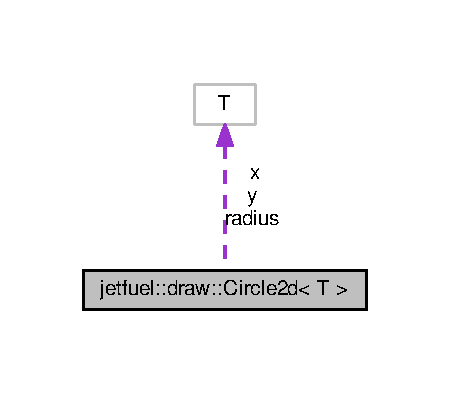
\includegraphics[width=216pt]{classjetfuel_1_1draw_1_1Circle2d__coll__graph}
\end{center}
\end{figure}
\subsection*{Public Member Functions}
\begin{DoxyCompactItemize}
\item 
\hyperlink{classjetfuel_1_1draw_1_1Circle2d_a265ed4234046e3a5fd669be4f39833bf}{Circle2d} ()
\begin{DoxyCompactList}\small\item\em Default constructor. \end{DoxyCompactList}\item 
\hyperlink{classjetfuel_1_1draw_1_1Circle2d_a46ba7b221cf32824a92014a856964e15}{Circle2d} (const T X, const T Y, const T Radius)
\begin{DoxyCompactList}\small\item\em Constructs a \hyperlink{classjetfuel_1_1draw_1_1Circle2d}{Circle2d} with a position and a radius. \end{DoxyCompactList}\item 
\hyperlink{classjetfuel_1_1draw_1_1Circle2d_abf30145c0e5f6602b735cebbff5ff12e}{Circle2d} (const \hyperlink{classjetfuel_1_1draw_1_1Vector2d}{Vector2d}$<$ T $>$ position, const T Radius)
\begin{DoxyCompactList}\small\item\em Constructs a \hyperlink{classjetfuel_1_1draw_1_1Circle2d}{Circle2d} with a position vector and a radius. \end{DoxyCompactList}\item 
\hyperlink{classjetfuel_1_1draw_1_1Vector2d}{Vector2d}$<$ T $>$ \hyperlink{classjetfuel_1_1draw_1_1Circle2d_ac29db892cec9356a9462fb1b78015a4a}{Get\+\_\+position} ()
\begin{DoxyCompactList}\small\item\em Gets this \hyperlink{classjetfuel_1_1draw_1_1Circle2d}{Circle2d}\textquotesingle{}s position. \end{DoxyCompactList}\item 
bool \hyperlink{classjetfuel_1_1draw_1_1Circle2d_aa34855d4f859792e7343608571af5501}{Has\+\_\+collided\+\_\+with\+\_\+circle} (\hyperlink{classjetfuel_1_1draw_1_1Circle2d}{Circle2d}$<$ T $>$ circle)
\begin{DoxyCompactList}\small\item\em Checks whether this \hyperlink{classjetfuel_1_1draw_1_1Circle2d}{Circle2d} collided with another \hyperlink{classjetfuel_1_1draw_1_1Circle2d}{Circle2d}. \end{DoxyCompactList}\item 
bool \hyperlink{classjetfuel_1_1draw_1_1Circle2d_a067f431a70a3df691223b955d4a1d573}{Has\+\_\+collided\+\_\+with\+\_\+rect} (\hyperlink{classjetfuel_1_1draw_1_1Rect2d}{Rect2d}$<$ T $>$ rect)
\begin{DoxyCompactList}\small\item\em Checks whether this \hyperlink{classjetfuel_1_1draw_1_1Circle2d}{Circle2d} has collided with a \hyperlink{classjetfuel_1_1draw_1_1Rect2d}{Rect2d}. \end{DoxyCompactList}\item 
bool \hyperlink{classjetfuel_1_1draw_1_1Circle2d_a51ddff1ce48a2433f108af1268abbcb3}{Has\+\_\+collided\+\_\+with\+\_\+mouse} ()
\begin{DoxyCompactList}\small\item\em Checks whether this \hyperlink{classjetfuel_1_1draw_1_1Circle2d}{Circle2d} has collided with the mouse. \end{DoxyCompactList}\end{DoxyCompactItemize}
\subsection*{Public Attributes}
\begin{DoxyCompactItemize}
\item 
T \hyperlink{classjetfuel_1_1draw_1_1Circle2d_a9aa0ccc7733d735950352373e2a72352}{x}
\begin{DoxyCompactList}\small\item\em member data /// \end{DoxyCompactList}\item 
\mbox{\Hypertarget{classjetfuel_1_1draw_1_1Circle2d_a720dee1fceb981cf5245bc82c2d5f8e1}\label{classjetfuel_1_1draw_1_1Circle2d_a720dee1fceb981cf5245bc82c2d5f8e1}} 
T \hyperlink{classjetfuel_1_1draw_1_1Circle2d_a720dee1fceb981cf5245bc82c2d5f8e1}{y}
\begin{DoxyCompactList}\small\item\em y position coordinate \end{DoxyCompactList}\item 
\mbox{\Hypertarget{classjetfuel_1_1draw_1_1Circle2d_ae5e10da97d4a857a6c14179f81bed159}\label{classjetfuel_1_1draw_1_1Circle2d_ae5e10da97d4a857a6c14179f81bed159}} 
T \hyperlink{classjetfuel_1_1draw_1_1Circle2d_ae5e10da97d4a857a6c14179f81bed159}{radius}
\begin{DoxyCompactList}\small\item\em circle radius \end{DoxyCompactList}\end{DoxyCompactItemize}


\subsection{Detailed Description}
\subsubsection*{template$<$class T$>$\newline
class jetfuel\+::draw\+::\+Circle2d$<$ T $>$}

A simple 2d circle manipulation class.

Code Example\+: 
\begin{DoxyCode}
\hyperlink{classjetfuel_1_1draw_1_1Circle2d}{jetfuel::draw::Circle2d\_int} mycircle(0,0,50);
\hyperlink{classjetfuel_1_1draw_1_1Circle__2d__shape}{jetfuel::draw::Circle\_2d\_shape} mydrawablecircle(mycircle);
\hyperlink{classjetfuel_1_1draw_1_1Scene__manager}{jetfuel::draw::Scene\_manager} scenemanager;
\hyperlink{classjetfuel_1_1draw_1_1Scene}{jetfuel::draw::Scene} scene1(1);

\textcolor{keywordflow}{if}(!scenemanager.\hyperlink{classjetfuel_1_1draw_1_1Scene__manager_a5113e9062c272a22d383ba872417ba31}{Create\_window}(\textcolor{stringliteral}{"example"},
                         \hyperlink{classjetfuel_1_1draw_1_1Vector2d}{jetfuel::draw::Vector2d\_int}(0,0),
                         \hyperlink{classjetfuel_1_1draw_1_1Vector2d}{jetfuel::draw::Vector2d\_int}(500,500)))\{
   std::cerr << \textcolor{stringliteral}{"[!]ERROR with creating sdl renderer!"} <<
   \textcolor{stringliteral}{"Error is:"} << SDL\_GetError() << \textcolor{stringliteral}{"\(\backslash\)n"};
\}

  \textcolor{keywordflow}{if}(!scenemanager.\hyperlink{classjetfuel_1_1draw_1_1Scene__manager_afafecd926ce5e4b2543a6d583a7d24b6}{Create\_renderer}())\{
       std::cerr << \textcolor{stringliteral}{"[!]ERROR with creating sdl renderer!"} <<
      \textcolor{stringliteral}{"Error is:"} << SDL\_GetError() << \textcolor{stringliteral}{"\(\backslash\)n"};
  \}

scenemanager.\hyperlink{classjetfuel_1_1draw_1_1Scene__manager_a770c163b88ba8427539ee182315ea989}{Switch\_current\_scene}(&scene1);

mydrawablecircle.Set\_color(\hyperlink{classjetfuel_1_1draw_1_1Color_a9c9781b9377310494e8af2a5fe524ab4}{jetfuel::draw::Color::Cyan});
scene1.Attach\_drawable(&mydrawablecircle,1S);

scenemanager.\hyperlink{classjetfuel_1_1draw_1_1Scene__manager_a8af9a3abfd5121b1b8556342de435773}{Draw\_current\_scene}();
\end{DoxyCode}
 

\subsection{Constructor \& Destructor Documentation}
\mbox{\Hypertarget{classjetfuel_1_1draw_1_1Circle2d_a265ed4234046e3a5fd669be4f39833bf}\label{classjetfuel_1_1draw_1_1Circle2d_a265ed4234046e3a5fd669be4f39833bf}} 
\index{jetfuel\+::draw\+::\+Circle2d@{jetfuel\+::draw\+::\+Circle2d}!Circle2d@{Circle2d}}
\index{Circle2d@{Circle2d}!jetfuel\+::draw\+::\+Circle2d@{jetfuel\+::draw\+::\+Circle2d}}
\subsubsection{\texorpdfstring{Circle2d()}{Circle2d()}\hspace{0.1cm}{\footnotesize\ttfamily [1/3]}}
{\footnotesize\ttfamily template$<$class T$>$ \\
\hyperlink{classjetfuel_1_1draw_1_1Circle2d}{jetfuel\+::draw\+::\+Circle2d}$<$ T $>$\+::\hyperlink{classjetfuel_1_1draw_1_1Circle2d}{Circle2d} (\begin{DoxyParamCaption}{ }\end{DoxyParamCaption})\hspace{0.3cm}{\ttfamily [inline]}}



Default constructor. 

Constructs a \hyperlink{classjetfuel_1_1draw_1_1Circle2d}{Circle2d} with all values set to zero. \mbox{\Hypertarget{classjetfuel_1_1draw_1_1Circle2d_a46ba7b221cf32824a92014a856964e15}\label{classjetfuel_1_1draw_1_1Circle2d_a46ba7b221cf32824a92014a856964e15}} 
\index{jetfuel\+::draw\+::\+Circle2d@{jetfuel\+::draw\+::\+Circle2d}!Circle2d@{Circle2d}}
\index{Circle2d@{Circle2d}!jetfuel\+::draw\+::\+Circle2d@{jetfuel\+::draw\+::\+Circle2d}}
\subsubsection{\texorpdfstring{Circle2d()}{Circle2d()}\hspace{0.1cm}{\footnotesize\ttfamily [2/3]}}
{\footnotesize\ttfamily template$<$class T$>$ \\
\hyperlink{classjetfuel_1_1draw_1_1Circle2d}{jetfuel\+::draw\+::\+Circle2d}$<$ T $>$\+::\hyperlink{classjetfuel_1_1draw_1_1Circle2d}{Circle2d} (\begin{DoxyParamCaption}\item[{const T}]{X,  }\item[{const T}]{Y,  }\item[{const T}]{Radius }\end{DoxyParamCaption})}



Constructs a \hyperlink{classjetfuel_1_1draw_1_1Circle2d}{Circle2d} with a position and a radius. 

Constructs a \hyperlink{classjetfuel_1_1draw_1_1Circle2d}{Circle2d} with a position and a radius.


\begin{DoxyParams}{Parameters}
{\em T} & X \\
\hline
{\em T} & Y \\
\hline
{\em T} & Radius \\
\hline
\end{DoxyParams}
\mbox{\Hypertarget{classjetfuel_1_1draw_1_1Circle2d_abf30145c0e5f6602b735cebbff5ff12e}\label{classjetfuel_1_1draw_1_1Circle2d_abf30145c0e5f6602b735cebbff5ff12e}} 
\index{jetfuel\+::draw\+::\+Circle2d@{jetfuel\+::draw\+::\+Circle2d}!Circle2d@{Circle2d}}
\index{Circle2d@{Circle2d}!jetfuel\+::draw\+::\+Circle2d@{jetfuel\+::draw\+::\+Circle2d}}
\subsubsection{\texorpdfstring{Circle2d()}{Circle2d()}\hspace{0.1cm}{\footnotesize\ttfamily [3/3]}}
{\footnotesize\ttfamily template$<$class T$>$ \\
\hyperlink{classjetfuel_1_1draw_1_1Circle2d}{jetfuel\+::draw\+::\+Circle2d}$<$ T $>$\+::\hyperlink{classjetfuel_1_1draw_1_1Circle2d}{Circle2d} (\begin{DoxyParamCaption}\item[{const \hyperlink{classjetfuel_1_1draw_1_1Vector2d}{Vector2d}$<$ T $>$}]{position,  }\item[{const T}]{Radius }\end{DoxyParamCaption})}



Constructs a \hyperlink{classjetfuel_1_1draw_1_1Circle2d}{Circle2d} with a position vector and a radius. 

Constructs a \hyperlink{classjetfuel_1_1draw_1_1Circle2d}{Circle2d} with a position vector and a radius.


\begin{DoxyParams}{Parameters}
{\em Vector2d$<$\+T$>$} & position \\
\hline
{\em T} & Radius \\
\hline
\end{DoxyParams}


\subsection{Member Function Documentation}
\mbox{\Hypertarget{classjetfuel_1_1draw_1_1Circle2d_ac29db892cec9356a9462fb1b78015a4a}\label{classjetfuel_1_1draw_1_1Circle2d_ac29db892cec9356a9462fb1b78015a4a}} 
\index{jetfuel\+::draw\+::\+Circle2d@{jetfuel\+::draw\+::\+Circle2d}!Get\+\_\+position@{Get\+\_\+position}}
\index{Get\+\_\+position@{Get\+\_\+position}!jetfuel\+::draw\+::\+Circle2d@{jetfuel\+::draw\+::\+Circle2d}}
\subsubsection{\texorpdfstring{Get\+\_\+position()}{Get\_position()}}
{\footnotesize\ttfamily template$<$class T$>$ \\
\hyperlink{classjetfuel_1_1draw_1_1Vector2d}{Vector2d}$<$T$>$ \hyperlink{classjetfuel_1_1draw_1_1Circle2d}{jetfuel\+::draw\+::\+Circle2d}$<$ T $>$\+::Get\+\_\+position (\begin{DoxyParamCaption}{ }\end{DoxyParamCaption})\hspace{0.3cm}{\ttfamily [inline]}}



Gets this \hyperlink{classjetfuel_1_1draw_1_1Circle2d}{Circle2d}\textquotesingle{}s position. 

Gets this \hyperlink{classjetfuel_1_1draw_1_1Circle2d}{Circle2d}\textquotesingle{}s position. \mbox{\Hypertarget{classjetfuel_1_1draw_1_1Circle2d_aa34855d4f859792e7343608571af5501}\label{classjetfuel_1_1draw_1_1Circle2d_aa34855d4f859792e7343608571af5501}} 
\index{jetfuel\+::draw\+::\+Circle2d@{jetfuel\+::draw\+::\+Circle2d}!Has\+\_\+collided\+\_\+with\+\_\+circle@{Has\+\_\+collided\+\_\+with\+\_\+circle}}
\index{Has\+\_\+collided\+\_\+with\+\_\+circle@{Has\+\_\+collided\+\_\+with\+\_\+circle}!jetfuel\+::draw\+::\+Circle2d@{jetfuel\+::draw\+::\+Circle2d}}
\subsubsection{\texorpdfstring{Has\+\_\+collided\+\_\+with\+\_\+circle()}{Has\_collided\_with\_circle()}}
{\footnotesize\ttfamily template$<$class T$>$ \\
bool \hyperlink{classjetfuel_1_1draw_1_1Circle2d}{jetfuel\+::draw\+::\+Circle2d}$<$ T $>$\+::Has\+\_\+collided\+\_\+with\+\_\+circle (\begin{DoxyParamCaption}\item[{\hyperlink{classjetfuel_1_1draw_1_1Circle2d}{Circle2d}$<$ T $>$}]{circle }\end{DoxyParamCaption})\hspace{0.3cm}{\ttfamily [inline]}}



Checks whether this \hyperlink{classjetfuel_1_1draw_1_1Circle2d}{Circle2d} collided with another \hyperlink{classjetfuel_1_1draw_1_1Circle2d}{Circle2d}. 

Checks whether this \hyperlink{classjetfuel_1_1draw_1_1Circle2d}{Circle2d} collided with another \hyperlink{classjetfuel_1_1draw_1_1Circle2d}{Circle2d}. If it has, then it will return a boolean of true. Otherwise, it will return a boolean of false.


\begin{DoxyParams}{Parameters}
{\em Circle2d$<$\+T$>$} & circle \\
\hline
\end{DoxyParams}
\mbox{\Hypertarget{classjetfuel_1_1draw_1_1Circle2d_a51ddff1ce48a2433f108af1268abbcb3}\label{classjetfuel_1_1draw_1_1Circle2d_a51ddff1ce48a2433f108af1268abbcb3}} 
\index{jetfuel\+::draw\+::\+Circle2d@{jetfuel\+::draw\+::\+Circle2d}!Has\+\_\+collided\+\_\+with\+\_\+mouse@{Has\+\_\+collided\+\_\+with\+\_\+mouse}}
\index{Has\+\_\+collided\+\_\+with\+\_\+mouse@{Has\+\_\+collided\+\_\+with\+\_\+mouse}!jetfuel\+::draw\+::\+Circle2d@{jetfuel\+::draw\+::\+Circle2d}}
\subsubsection{\texorpdfstring{Has\+\_\+collided\+\_\+with\+\_\+mouse()}{Has\_collided\_with\_mouse()}}
{\footnotesize\ttfamily template$<$class T$>$ \\
bool \hyperlink{classjetfuel_1_1draw_1_1Circle2d}{jetfuel\+::draw\+::\+Circle2d}$<$ T $>$\+::Has\+\_\+collided\+\_\+with\+\_\+mouse (\begin{DoxyParamCaption}{ }\end{DoxyParamCaption})\hspace{0.3cm}{\ttfamily [inline]}}



Checks whether this \hyperlink{classjetfuel_1_1draw_1_1Circle2d}{Circle2d} has collided with the mouse. 

Checks whether this \hyperlink{classjetfuel_1_1draw_1_1Circle2d}{Circle2d} has collided with the mouse. If it has, then this function will return a boolean of true. Otherwise, it will return a boolean of false. \mbox{\Hypertarget{classjetfuel_1_1draw_1_1Circle2d_a067f431a70a3df691223b955d4a1d573}\label{classjetfuel_1_1draw_1_1Circle2d_a067f431a70a3df691223b955d4a1d573}} 
\index{jetfuel\+::draw\+::\+Circle2d@{jetfuel\+::draw\+::\+Circle2d}!Has\+\_\+collided\+\_\+with\+\_\+rect@{Has\+\_\+collided\+\_\+with\+\_\+rect}}
\index{Has\+\_\+collided\+\_\+with\+\_\+rect@{Has\+\_\+collided\+\_\+with\+\_\+rect}!jetfuel\+::draw\+::\+Circle2d@{jetfuel\+::draw\+::\+Circle2d}}
\subsubsection{\texorpdfstring{Has\+\_\+collided\+\_\+with\+\_\+rect()}{Has\_collided\_with\_rect()}}
{\footnotesize\ttfamily template$<$class T$>$ \\
bool \hyperlink{classjetfuel_1_1draw_1_1Circle2d}{jetfuel\+::draw\+::\+Circle2d}$<$ T $>$\+::Has\+\_\+collided\+\_\+with\+\_\+rect (\begin{DoxyParamCaption}\item[{\hyperlink{classjetfuel_1_1draw_1_1Rect2d}{Rect2d}$<$ T $>$}]{rect }\end{DoxyParamCaption})\hspace{0.3cm}{\ttfamily [inline]}}



Checks whether this \hyperlink{classjetfuel_1_1draw_1_1Circle2d}{Circle2d} has collided with a \hyperlink{classjetfuel_1_1draw_1_1Rect2d}{Rect2d}. 

Checks whether this \hyperlink{classjetfuel_1_1draw_1_1Circle2d}{Circle2d} has collided with a \hyperlink{classjetfuel_1_1draw_1_1Rect2d}{Rect2d}. If it has, then this function will return a boolean of true. Otherwise, it will return a boolean of false.


\begin{DoxyParams}{Parameters}
{\em Rect2d$<$\+T$>$} & rect \\
\hline
\end{DoxyParams}


\subsection{Member Data Documentation}
\mbox{\Hypertarget{classjetfuel_1_1draw_1_1Circle2d_a9aa0ccc7733d735950352373e2a72352}\label{classjetfuel_1_1draw_1_1Circle2d_a9aa0ccc7733d735950352373e2a72352}} 
\index{jetfuel\+::draw\+::\+Circle2d@{jetfuel\+::draw\+::\+Circle2d}!x@{x}}
\index{x@{x}!jetfuel\+::draw\+::\+Circle2d@{jetfuel\+::draw\+::\+Circle2d}}
\subsubsection{\texorpdfstring{x}{x}}
{\footnotesize\ttfamily template$<$class T$>$ \\
T \hyperlink{classjetfuel_1_1draw_1_1Circle2d}{jetfuel\+::draw\+::\+Circle2d}$<$ T $>$\+::x}



member data /// 

x position coordinate 

The documentation for this class was generated from the following file\+:\begin{DoxyCompactItemize}
\item 
include/jetfueldraw/circle2d.\+h\end{DoxyCompactItemize}

\hypertarget{classjetfuel_1_1draw_1_1Circle__2d__shape}{}\section{jetfuel\+:\+:draw\+:\+:Circle\+\_\+2d\+\_\+shape Class Reference}
\label{classjetfuel_1_1draw_1_1Circle__2d__shape}\index{jetfuel\+::draw\+::\+Circle\+\_\+2d\+\_\+shape@{jetfuel\+::draw\+::\+Circle\+\_\+2d\+\_\+shape}}


{\ttfamily \#include $<$circle2dshape.\+h$>$}



Inheritance diagram for jetfuel\+:\+:draw\+:\+:Circle\+\_\+2d\+\_\+shape\+:\nopagebreak
\begin{figure}[H]
\begin{center}
\leavevmode
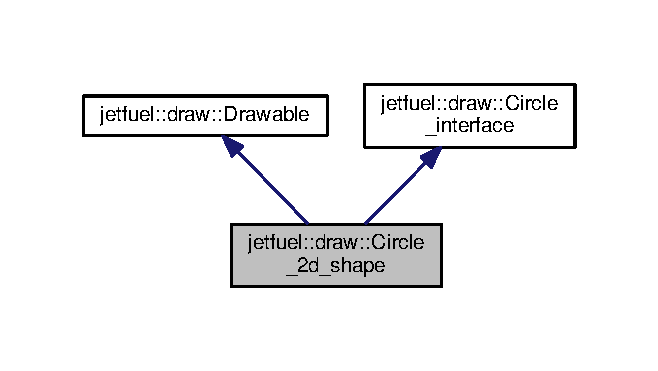
\includegraphics[width=316pt]{classjetfuel_1_1draw_1_1Circle__2d__shape__inherit__graph}
\end{center}
\end{figure}


Collaboration diagram for jetfuel\+:\+:draw\+:\+:Circle\+\_\+2d\+\_\+shape\+:\nopagebreak
\begin{figure}[H]
\begin{center}
\leavevmode
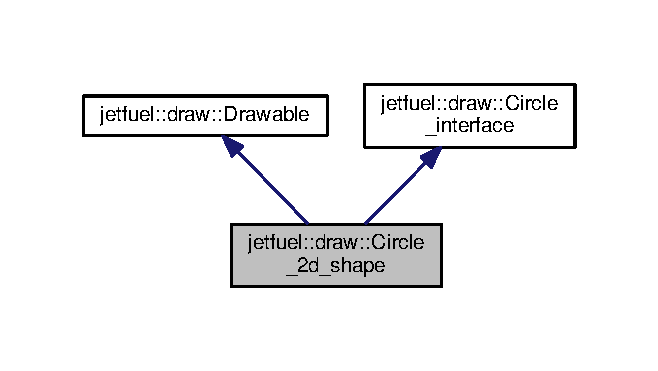
\includegraphics[width=316pt]{classjetfuel_1_1draw_1_1Circle__2d__shape__coll__graph}
\end{center}
\end{figure}
\subsection*{Classes}
\begin{DoxyCompactItemize}
\item 
struct \hyperlink{structjetfuel_1_1draw_1_1Circle__2d__shape_1_1Circle__2d__shape__characteristics}{Circle\+\_\+2d\+\_\+shape\+\_\+characteristics}
\end{DoxyCompactItemize}
\subsection*{Public Member Functions}
\begin{DoxyCompactItemize}
\item 
\hyperlink{classjetfuel_1_1draw_1_1Circle__2d__shape_a0c6320cecb7ee7bfff185f4607a5f830}{Circle\+\_\+2d\+\_\+shape} ()
\begin{DoxyCompactList}\small\item\em Default constructor. \end{DoxyCompactList}\item 
\hyperlink{classjetfuel_1_1draw_1_1Circle__2d__shape_ad2be0a546c65e671a92dd30e20461afe}{Circle\+\_\+2d\+\_\+shape} (const \hyperlink{classjetfuel_1_1draw_1_1Circle2d}{Circle2d\+\_\+int} circletodraw)
\begin{DoxyCompactList}\small\item\em Constructs a \hyperlink{classjetfuel_1_1draw_1_1Circle__2d__shape}{Circle\+\_\+2d\+\_\+shape} with a Circle2d\+\_\+int. \end{DoxyCompactList}\item 
\hyperlink{classjetfuel_1_1draw_1_1Vector2d}{Vector2d\+\_\+int} \hyperlink{classjetfuel_1_1draw_1_1Circle__2d__shape_a99b93544660c7f5b11cf8f0169e8fec1}{Get\+\_\+position} () override
\begin{DoxyCompactList}\small\item\em Gets the \hyperlink{classjetfuel_1_1draw_1_1Circle__2d__shape}{Circle\+\_\+2d\+\_\+shape}\textquotesingle{}s position. \end{DoxyCompactList}\item 
void \hyperlink{classjetfuel_1_1draw_1_1Circle__2d__shape_a551b38063543823483f560bf3eebcd2c}{Set\+\_\+position} (const \hyperlink{classjetfuel_1_1draw_1_1Vector2d}{Vector2d\+\_\+int} position) override
\begin{DoxyCompactList}\small\item\em Sets the \hyperlink{classjetfuel_1_1draw_1_1Circle__2d__shape}{Circle\+\_\+2d\+\_\+shape}\textquotesingle{}s position. \end{DoxyCompactList}\item 
int \hyperlink{classjetfuel_1_1draw_1_1Circle__2d__shape_ae3686026f21348b28769d7a89f59c071}{Get\+\_\+radius} () const
\begin{DoxyCompactList}\small\item\em Gets the \hyperlink{classjetfuel_1_1draw_1_1Circle__2d__shape}{Circle\+\_\+2d\+\_\+shape}\textquotesingle{}s radius. \end{DoxyCompactList}\item 
void \hyperlink{classjetfuel_1_1draw_1_1Circle__2d__shape_a100c20cab54eaaafca78147854b0a3c3}{Set\+\_\+radius} (const int radius)
\begin{DoxyCompactList}\small\item\em Sets the \hyperlink{classjetfuel_1_1draw_1_1Circle__2d__shape}{Circle\+\_\+2d\+\_\+shape}\textquotesingle{}s radius. \end{DoxyCompactList}\item 
\hyperlink{classjetfuel_1_1draw_1_1Circle2d}{Circle2d\+\_\+int} \hyperlink{classjetfuel_1_1draw_1_1Circle__2d__shape_ab188ed6716dff22d0498a01ac1e93d90}{Get\+\_\+circle\+\_\+to\+\_\+draw} () override
\begin{DoxyCompactList}\small\item\em Gets the circle to draw. \end{DoxyCompactList}\item 
bool \hyperlink{classjetfuel_1_1draw_1_1Circle__2d__shape_af5e8ebfd4c5102e25263500c0a2075b9}{Get\+\_\+anti\+\_\+aliasing\+\_\+status} () const
\begin{DoxyCompactList}\small\item\em Gets the anti aliasing status. \end{DoxyCompactList}\item 
void \hyperlink{classjetfuel_1_1draw_1_1Circle__2d__shape_a2af81e6479bc9d55b7df7e3c0a392630}{Set\+\_\+anti\+\_\+aliasing\+\_\+status} (const bool aastatus)
\begin{DoxyCompactList}\small\item\em Sets the anti aliasing status. \end{DoxyCompactList}\item 
bool \hyperlink{classjetfuel_1_1draw_1_1Circle__2d__shape_af742bd69519677da00692b9c8b7b0d74}{Get\+\_\+filled\+\_\+circle\+\_\+status} () const
\begin{DoxyCompactList}\small\item\em Gets whether the circle is being filled in. \end{DoxyCompactList}\item 
void \hyperlink{classjetfuel_1_1draw_1_1Circle__2d__shape_a027d4640ee52708f5fa853f20ba2f899}{Set\+\_\+filled\+\_\+circle\+\_\+status} (const bool filledincircle)
\begin{DoxyCompactList}\small\item\em Sets whether the circle will be filled in. \end{DoxyCompactList}\item 
\hyperlink{classjetfuel_1_1draw_1_1Color}{Color} \hyperlink{classjetfuel_1_1draw_1_1Circle__2d__shape_ad7953fa383fdffedf6cdf9d6a3d9a1bb}{Get\+\_\+color} () const
\begin{DoxyCompactList}\small\item\em Gets the global color of this circle. \end{DoxyCompactList}\item 
void \hyperlink{classjetfuel_1_1draw_1_1Circle__2d__shape_a20ac0647e90c629f347e3c65a0315220}{Set\+\_\+color} (const \hyperlink{classjetfuel_1_1draw_1_1Color}{Color} color)
\begin{DoxyCompactList}\small\item\em Sets the global color of this circle. \end{DoxyCompactList}\item 
bool \hyperlink{classjetfuel_1_1draw_1_1Circle__2d__shape_a8be660f3cd624dc077d9003ee3b37212}{Draw} () override
\begin{DoxyCompactList}\small\item\em Draws the circle. \end{DoxyCompactList}\end{DoxyCompactItemize}
\subsection*{Additional Inherited Members}


\subsection{Detailed Description}
A drawable 2d circle shape to be shown to the player.

Code Example\+: 
\begin{DoxyCode}
\hyperlink{classjetfuel_1_1draw_1_1Circle2d}{jetfuel::draw::Circle2d\_int} mycircle(0,0,50);
\hyperlink{classjetfuel_1_1draw_1_1Circle__2d__shape}{jetfuel::draw::Circle\_2d\_shape} mydrawablecircle(mycircle);
\hyperlink{classjetfuel_1_1draw_1_1Scene__manager}{jetfuel::draw::Scene\_manager} scenemanager;
\hyperlink{classjetfuel_1_1draw_1_1Scene}{jetfuel::draw::Scene} scene1(1);

\textcolor{keywordflow}{if}(!scenemanager.\hyperlink{classjetfuel_1_1draw_1_1Scene__manager_a5113e9062c272a22d383ba872417ba31}{Create\_window}(\textcolor{stringliteral}{"example"},
                         \hyperlink{classjetfuel_1_1draw_1_1Vector2d}{jetfuel::draw::Vector2d\_int}(0,0),
                         \hyperlink{classjetfuel_1_1draw_1_1Vector2d}{jetfuel::draw::Vector2d\_int}(500,500)))\{
   std::cerr << \textcolor{stringliteral}{"[!]ERROR with creating sdl renderer!"} <<
   \textcolor{stringliteral}{"Error is:"} << SDL\_GetError() << \textcolor{stringliteral}{"\(\backslash\)n"};
\}

  \textcolor{keywordflow}{if}(!scenemanager.\hyperlink{classjetfuel_1_1draw_1_1Scene__manager_afafecd926ce5e4b2543a6d583a7d24b6}{Create\_renderer}())\{
       std::cerr << \textcolor{stringliteral}{"[!]ERROR with creating sdl renderer!"} <<
      \textcolor{stringliteral}{"Error is:"} << SDL\_GetError() << \textcolor{stringliteral}{"\(\backslash\)n"};
  \}

scenemanager.\hyperlink{classjetfuel_1_1draw_1_1Scene__manager_a770c163b88ba8427539ee182315ea989}{Switch\_current\_scene}(&scene1);

mydrawablecircle.Set\_color(\hyperlink{classjetfuel_1_1draw_1_1Color_a9c9781b9377310494e8af2a5fe524ab4}{jetfuel::draw::Color::Cyan});
scene1.Attach\_drawable(&mydrawablecircle,1S);

scenemanager.\hyperlink{classjetfuel_1_1draw_1_1Scene__manager_a8af9a3abfd5121b1b8556342de435773}{Draw\_current\_scene}();
\end{DoxyCode}
 

\subsection{Constructor \& Destructor Documentation}
\mbox{\Hypertarget{classjetfuel_1_1draw_1_1Circle__2d__shape_a0c6320cecb7ee7bfff185f4607a5f830}\label{classjetfuel_1_1draw_1_1Circle__2d__shape_a0c6320cecb7ee7bfff185f4607a5f830}} 
\index{jetfuel\+::draw\+::\+Circle\+\_\+2d\+\_\+shape@{jetfuel\+::draw\+::\+Circle\+\_\+2d\+\_\+shape}!Circle\+\_\+2d\+\_\+shape@{Circle\+\_\+2d\+\_\+shape}}
\index{Circle\+\_\+2d\+\_\+shape@{Circle\+\_\+2d\+\_\+shape}!jetfuel\+::draw\+::\+Circle\+\_\+2d\+\_\+shape@{jetfuel\+::draw\+::\+Circle\+\_\+2d\+\_\+shape}}
\subsubsection{\texorpdfstring{Circle\+\_\+2d\+\_\+shape()}{Circle\_2d\_shape()}\hspace{0.1cm}{\footnotesize\ttfamily [1/2]}}
{\footnotesize\ttfamily jetfuel\+::draw\+::\+Circle\+\_\+2d\+\_\+shape\+::\+Circle\+\_\+2d\+\_\+shape (\begin{DoxyParamCaption}{ }\end{DoxyParamCaption})\hspace{0.3cm}{\ttfamily [inline]}}



Default constructor. 

Constructs an empty \hyperlink{classjetfuel_1_1draw_1_1Circle__2d__shape}{Circle\+\_\+2d\+\_\+shape}. \mbox{\Hypertarget{classjetfuel_1_1draw_1_1Circle__2d__shape_ad2be0a546c65e671a92dd30e20461afe}\label{classjetfuel_1_1draw_1_1Circle__2d__shape_ad2be0a546c65e671a92dd30e20461afe}} 
\index{jetfuel\+::draw\+::\+Circle\+\_\+2d\+\_\+shape@{jetfuel\+::draw\+::\+Circle\+\_\+2d\+\_\+shape}!Circle\+\_\+2d\+\_\+shape@{Circle\+\_\+2d\+\_\+shape}}
\index{Circle\+\_\+2d\+\_\+shape@{Circle\+\_\+2d\+\_\+shape}!jetfuel\+::draw\+::\+Circle\+\_\+2d\+\_\+shape@{jetfuel\+::draw\+::\+Circle\+\_\+2d\+\_\+shape}}
\subsubsection{\texorpdfstring{Circle\+\_\+2d\+\_\+shape()}{Circle\_2d\_shape()}\hspace{0.1cm}{\footnotesize\ttfamily [2/2]}}
{\footnotesize\ttfamily jetfuel\+::draw\+::\+Circle\+\_\+2d\+\_\+shape\+::\+Circle\+\_\+2d\+\_\+shape (\begin{DoxyParamCaption}\item[{const \hyperlink{classjetfuel_1_1draw_1_1Circle2d}{Circle2d\+\_\+int}}]{circletodraw }\end{DoxyParamCaption})}



Constructs a \hyperlink{classjetfuel_1_1draw_1_1Circle__2d__shape}{Circle\+\_\+2d\+\_\+shape} with a Circle2d\+\_\+int. 

Constructs a \hyperlink{classjetfuel_1_1draw_1_1Circle__2d__shape}{Circle\+\_\+2d\+\_\+shape} with a Circle2d\+\_\+int.


\begin{DoxyParams}{Parameters}
{\em Circle2d\+\_\+int} & circletodraw \\
\hline
\end{DoxyParams}


\subsection{Member Function Documentation}
\mbox{\Hypertarget{classjetfuel_1_1draw_1_1Circle__2d__shape_a8be660f3cd624dc077d9003ee3b37212}\label{classjetfuel_1_1draw_1_1Circle__2d__shape_a8be660f3cd624dc077d9003ee3b37212}} 
\index{jetfuel\+::draw\+::\+Circle\+\_\+2d\+\_\+shape@{jetfuel\+::draw\+::\+Circle\+\_\+2d\+\_\+shape}!Draw@{Draw}}
\index{Draw@{Draw}!jetfuel\+::draw\+::\+Circle\+\_\+2d\+\_\+shape@{jetfuel\+::draw\+::\+Circle\+\_\+2d\+\_\+shape}}
\subsubsection{\texorpdfstring{Draw()}{Draw()}}
{\footnotesize\ttfamily bool jetfuel\+::draw\+::\+Circle\+\_\+2d\+\_\+shape\+::\+Draw (\begin{DoxyParamCaption}{ }\end{DoxyParamCaption})\hspace{0.3cm}{\ttfamily [override]}, {\ttfamily [virtual]}}



Draws the circle. 

Draws the circle. It is recommended to let \hyperlink{classjetfuel_1_1draw_1_1Scene}{jetfuel\+::draw\+::\+Scene} and \hyperlink{classjetfuel_1_1draw_1_1Scene__manager}{jetfuel\+::draw\+::\+Scene\+\_\+manager} call this, and not by yourself. 

Implements \hyperlink{classjetfuel_1_1draw_1_1Drawable_a1a072070322965ce9411ee6e7c311c56}{jetfuel\+::draw\+::\+Drawable}.

\mbox{\Hypertarget{classjetfuel_1_1draw_1_1Circle__2d__shape_af5e8ebfd4c5102e25263500c0a2075b9}\label{classjetfuel_1_1draw_1_1Circle__2d__shape_af5e8ebfd4c5102e25263500c0a2075b9}} 
\index{jetfuel\+::draw\+::\+Circle\+\_\+2d\+\_\+shape@{jetfuel\+::draw\+::\+Circle\+\_\+2d\+\_\+shape}!Get\+\_\+anti\+\_\+aliasing\+\_\+status@{Get\+\_\+anti\+\_\+aliasing\+\_\+status}}
\index{Get\+\_\+anti\+\_\+aliasing\+\_\+status@{Get\+\_\+anti\+\_\+aliasing\+\_\+status}!jetfuel\+::draw\+::\+Circle\+\_\+2d\+\_\+shape@{jetfuel\+::draw\+::\+Circle\+\_\+2d\+\_\+shape}}
\subsubsection{\texorpdfstring{Get\+\_\+anti\+\_\+aliasing\+\_\+status()}{Get\_anti\_aliasing\_status()}}
{\footnotesize\ttfamily bool jetfuel\+::draw\+::\+Circle\+\_\+2d\+\_\+shape\+::\+Get\+\_\+anti\+\_\+aliasing\+\_\+status (\begin{DoxyParamCaption}{ }\end{DoxyParamCaption}) const\hspace{0.3cm}{\ttfamily [inline]}}



Gets the anti aliasing status. 

Gets the anti aliasing status. If this is set to true, it means that anti aliasing is enabled on this circle, and, theoretically, it will render much slower. For this reason, you should not enable this unless the player specifies to enable it, or you are confident that players running your game will not suffer any major performance loss. This anti aliasing status will O\+N\+LY come into effect if the circle being drawn is N\+OT filled. \mbox{\Hypertarget{classjetfuel_1_1draw_1_1Circle__2d__shape_ab188ed6716dff22d0498a01ac1e93d90}\label{classjetfuel_1_1draw_1_1Circle__2d__shape_ab188ed6716dff22d0498a01ac1e93d90}} 
\index{jetfuel\+::draw\+::\+Circle\+\_\+2d\+\_\+shape@{jetfuel\+::draw\+::\+Circle\+\_\+2d\+\_\+shape}!Get\+\_\+circle\+\_\+to\+\_\+draw@{Get\+\_\+circle\+\_\+to\+\_\+draw}}
\index{Get\+\_\+circle\+\_\+to\+\_\+draw@{Get\+\_\+circle\+\_\+to\+\_\+draw}!jetfuel\+::draw\+::\+Circle\+\_\+2d\+\_\+shape@{jetfuel\+::draw\+::\+Circle\+\_\+2d\+\_\+shape}}
\subsubsection{\texorpdfstring{Get\+\_\+circle\+\_\+to\+\_\+draw()}{Get\_circle\_to\_draw()}}
{\footnotesize\ttfamily \hyperlink{classjetfuel_1_1draw_1_1Circle2d}{Circle2d\+\_\+int} jetfuel\+::draw\+::\+Circle\+\_\+2d\+\_\+shape\+::\+Get\+\_\+circle\+\_\+to\+\_\+draw (\begin{DoxyParamCaption}{ }\end{DoxyParamCaption})\hspace{0.3cm}{\ttfamily [inline]}, {\ttfamily [override]}, {\ttfamily [virtual]}}



Gets the circle to draw. 

Gets the circle to draw that will be drawn upon the function \hyperlink{classjetfuel_1_1draw_1_1Circle__2d__shape_a8be660f3cd624dc077d9003ee3b37212}{Draw()} being called. 

Implements \hyperlink{classjetfuel_1_1draw_1_1Circle__interface_a992a93bc130288ec4c9c4d2fa4203341}{jetfuel\+::draw\+::\+Circle\+\_\+interface}.

\mbox{\Hypertarget{classjetfuel_1_1draw_1_1Circle__2d__shape_ad7953fa383fdffedf6cdf9d6a3d9a1bb}\label{classjetfuel_1_1draw_1_1Circle__2d__shape_ad7953fa383fdffedf6cdf9d6a3d9a1bb}} 
\index{jetfuel\+::draw\+::\+Circle\+\_\+2d\+\_\+shape@{jetfuel\+::draw\+::\+Circle\+\_\+2d\+\_\+shape}!Get\+\_\+color@{Get\+\_\+color}}
\index{Get\+\_\+color@{Get\+\_\+color}!jetfuel\+::draw\+::\+Circle\+\_\+2d\+\_\+shape@{jetfuel\+::draw\+::\+Circle\+\_\+2d\+\_\+shape}}
\subsubsection{\texorpdfstring{Get\+\_\+color()}{Get\_color()}}
{\footnotesize\ttfamily \hyperlink{classjetfuel_1_1draw_1_1Color}{Color} jetfuel\+::draw\+::\+Circle\+\_\+2d\+\_\+shape\+::\+Get\+\_\+color (\begin{DoxyParamCaption}{ }\end{DoxyParamCaption}) const\hspace{0.3cm}{\ttfamily [inline]}}



Gets the global color of this circle. 

Gets the global color of this circle that will be displayed to the player upon \hyperlink{classjetfuel_1_1draw_1_1Circle__2d__shape_a8be660f3cd624dc077d9003ee3b37212}{Draw()} being called. \mbox{\Hypertarget{classjetfuel_1_1draw_1_1Circle__2d__shape_af742bd69519677da00692b9c8b7b0d74}\label{classjetfuel_1_1draw_1_1Circle__2d__shape_af742bd69519677da00692b9c8b7b0d74}} 
\index{jetfuel\+::draw\+::\+Circle\+\_\+2d\+\_\+shape@{jetfuel\+::draw\+::\+Circle\+\_\+2d\+\_\+shape}!Get\+\_\+filled\+\_\+circle\+\_\+status@{Get\+\_\+filled\+\_\+circle\+\_\+status}}
\index{Get\+\_\+filled\+\_\+circle\+\_\+status@{Get\+\_\+filled\+\_\+circle\+\_\+status}!jetfuel\+::draw\+::\+Circle\+\_\+2d\+\_\+shape@{jetfuel\+::draw\+::\+Circle\+\_\+2d\+\_\+shape}}
\subsubsection{\texorpdfstring{Get\+\_\+filled\+\_\+circle\+\_\+status()}{Get\_filled\_circle\_status()}}
{\footnotesize\ttfamily bool jetfuel\+::draw\+::\+Circle\+\_\+2d\+\_\+shape\+::\+Get\+\_\+filled\+\_\+circle\+\_\+status (\begin{DoxyParamCaption}{ }\end{DoxyParamCaption}) const\hspace{0.3cm}{\ttfamily [inline]}}



Gets whether the circle is being filled in. 

Gets whether the circle is being filled in. \mbox{\Hypertarget{classjetfuel_1_1draw_1_1Circle__2d__shape_a99b93544660c7f5b11cf8f0169e8fec1}\label{classjetfuel_1_1draw_1_1Circle__2d__shape_a99b93544660c7f5b11cf8f0169e8fec1}} 
\index{jetfuel\+::draw\+::\+Circle\+\_\+2d\+\_\+shape@{jetfuel\+::draw\+::\+Circle\+\_\+2d\+\_\+shape}!Get\+\_\+position@{Get\+\_\+position}}
\index{Get\+\_\+position@{Get\+\_\+position}!jetfuel\+::draw\+::\+Circle\+\_\+2d\+\_\+shape@{jetfuel\+::draw\+::\+Circle\+\_\+2d\+\_\+shape}}
\subsubsection{\texorpdfstring{Get\+\_\+position()}{Get\_position()}}
{\footnotesize\ttfamily \hyperlink{classjetfuel_1_1draw_1_1Vector2d}{Vector2d\+\_\+int} jetfuel\+::draw\+::\+Circle\+\_\+2d\+\_\+shape\+::\+Get\+\_\+position (\begin{DoxyParamCaption}{ }\end{DoxyParamCaption})\hspace{0.3cm}{\ttfamily [inline]}, {\ttfamily [override]}, {\ttfamily [virtual]}}



Gets the \hyperlink{classjetfuel_1_1draw_1_1Circle__2d__shape}{Circle\+\_\+2d\+\_\+shape}\textquotesingle{}s position. 

Gets the \hyperlink{classjetfuel_1_1draw_1_1Circle__2d__shape}{Circle\+\_\+2d\+\_\+shape}\textquotesingle{}s position. 

Reimplemented from \hyperlink{classjetfuel_1_1draw_1_1Drawable_ae7ebd30d66db2c8a5d5371cbcf0023fc}{jetfuel\+::draw\+::\+Drawable}.

\mbox{\Hypertarget{classjetfuel_1_1draw_1_1Circle__2d__shape_ae3686026f21348b28769d7a89f59c071}\label{classjetfuel_1_1draw_1_1Circle__2d__shape_ae3686026f21348b28769d7a89f59c071}} 
\index{jetfuel\+::draw\+::\+Circle\+\_\+2d\+\_\+shape@{jetfuel\+::draw\+::\+Circle\+\_\+2d\+\_\+shape}!Get\+\_\+radius@{Get\+\_\+radius}}
\index{Get\+\_\+radius@{Get\+\_\+radius}!jetfuel\+::draw\+::\+Circle\+\_\+2d\+\_\+shape@{jetfuel\+::draw\+::\+Circle\+\_\+2d\+\_\+shape}}
\subsubsection{\texorpdfstring{Get\+\_\+radius()}{Get\_radius()}}
{\footnotesize\ttfamily int jetfuel\+::draw\+::\+Circle\+\_\+2d\+\_\+shape\+::\+Get\+\_\+radius (\begin{DoxyParamCaption}{ }\end{DoxyParamCaption}) const\hspace{0.3cm}{\ttfamily [inline]}}



Gets the \hyperlink{classjetfuel_1_1draw_1_1Circle__2d__shape}{Circle\+\_\+2d\+\_\+shape}\textquotesingle{}s radius. 

Gets the \hyperlink{classjetfuel_1_1draw_1_1Circle__2d__shape}{Circle\+\_\+2d\+\_\+shape}\textquotesingle{}s radius. \mbox{\Hypertarget{classjetfuel_1_1draw_1_1Circle__2d__shape_a2af81e6479bc9d55b7df7e3c0a392630}\label{classjetfuel_1_1draw_1_1Circle__2d__shape_a2af81e6479bc9d55b7df7e3c0a392630}} 
\index{jetfuel\+::draw\+::\+Circle\+\_\+2d\+\_\+shape@{jetfuel\+::draw\+::\+Circle\+\_\+2d\+\_\+shape}!Set\+\_\+anti\+\_\+aliasing\+\_\+status@{Set\+\_\+anti\+\_\+aliasing\+\_\+status}}
\index{Set\+\_\+anti\+\_\+aliasing\+\_\+status@{Set\+\_\+anti\+\_\+aliasing\+\_\+status}!jetfuel\+::draw\+::\+Circle\+\_\+2d\+\_\+shape@{jetfuel\+::draw\+::\+Circle\+\_\+2d\+\_\+shape}}
\subsubsection{\texorpdfstring{Set\+\_\+anti\+\_\+aliasing\+\_\+status()}{Set\_anti\_aliasing\_status()}}
{\footnotesize\ttfamily void jetfuel\+::draw\+::\+Circle\+\_\+2d\+\_\+shape\+::\+Set\+\_\+anti\+\_\+aliasing\+\_\+status (\begin{DoxyParamCaption}\item[{const bool}]{aastatus }\end{DoxyParamCaption})\hspace{0.3cm}{\ttfamily [inline]}}



Sets the anti aliasing status. 

Sets the anti aliasing status. If this is set to true, it means that anti aliasing is enabled on this circle, and, theoretically, it will render much slower. For this reason, you should not enable this unless the player wants to enable it, or you are confident that players running your game will not suffer any major performance loss. This anti aliasing status will O\+N\+LY come into effect if the circle being drawn is N\+OT filled.


\begin{DoxyParams}{Parameters}
{\em bool} & aastatus \\
\hline
\end{DoxyParams}
\mbox{\Hypertarget{classjetfuel_1_1draw_1_1Circle__2d__shape_a20ac0647e90c629f347e3c65a0315220}\label{classjetfuel_1_1draw_1_1Circle__2d__shape_a20ac0647e90c629f347e3c65a0315220}} 
\index{jetfuel\+::draw\+::\+Circle\+\_\+2d\+\_\+shape@{jetfuel\+::draw\+::\+Circle\+\_\+2d\+\_\+shape}!Set\+\_\+color@{Set\+\_\+color}}
\index{Set\+\_\+color@{Set\+\_\+color}!jetfuel\+::draw\+::\+Circle\+\_\+2d\+\_\+shape@{jetfuel\+::draw\+::\+Circle\+\_\+2d\+\_\+shape}}
\subsubsection{\texorpdfstring{Set\+\_\+color()}{Set\_color()}}
{\footnotesize\ttfamily void jetfuel\+::draw\+::\+Circle\+\_\+2d\+\_\+shape\+::\+Set\+\_\+color (\begin{DoxyParamCaption}\item[{const \hyperlink{classjetfuel_1_1draw_1_1Color}{Color}}]{color }\end{DoxyParamCaption})\hspace{0.3cm}{\ttfamily [inline]}}



Sets the global color of this circle. 

Sets the global color of this circle that will be displayed to the player upon \hyperlink{classjetfuel_1_1draw_1_1Circle__2d__shape_a8be660f3cd624dc077d9003ee3b37212}{Draw()} being called.


\begin{DoxyParams}{Parameters}
{\em \hyperlink{classjetfuel_1_1draw_1_1Color}{Color}} & color \\
\hline
\end{DoxyParams}
\mbox{\Hypertarget{classjetfuel_1_1draw_1_1Circle__2d__shape_a027d4640ee52708f5fa853f20ba2f899}\label{classjetfuel_1_1draw_1_1Circle__2d__shape_a027d4640ee52708f5fa853f20ba2f899}} 
\index{jetfuel\+::draw\+::\+Circle\+\_\+2d\+\_\+shape@{jetfuel\+::draw\+::\+Circle\+\_\+2d\+\_\+shape}!Set\+\_\+filled\+\_\+circle\+\_\+status@{Set\+\_\+filled\+\_\+circle\+\_\+status}}
\index{Set\+\_\+filled\+\_\+circle\+\_\+status@{Set\+\_\+filled\+\_\+circle\+\_\+status}!jetfuel\+::draw\+::\+Circle\+\_\+2d\+\_\+shape@{jetfuel\+::draw\+::\+Circle\+\_\+2d\+\_\+shape}}
\subsubsection{\texorpdfstring{Set\+\_\+filled\+\_\+circle\+\_\+status()}{Set\_filled\_circle\_status()}}
{\footnotesize\ttfamily void jetfuel\+::draw\+::\+Circle\+\_\+2d\+\_\+shape\+::\+Set\+\_\+filled\+\_\+circle\+\_\+status (\begin{DoxyParamCaption}\item[{const bool}]{filledincircle }\end{DoxyParamCaption})\hspace{0.3cm}{\ttfamily [inline]}}



Sets whether the circle will be filled in. 

Sets whether the circle will be filled in.


\begin{DoxyParams}{Parameters}
{\em bool} & filledincircle \\
\hline
\end{DoxyParams}
\mbox{\Hypertarget{classjetfuel_1_1draw_1_1Circle__2d__shape_a551b38063543823483f560bf3eebcd2c}\label{classjetfuel_1_1draw_1_1Circle__2d__shape_a551b38063543823483f560bf3eebcd2c}} 
\index{jetfuel\+::draw\+::\+Circle\+\_\+2d\+\_\+shape@{jetfuel\+::draw\+::\+Circle\+\_\+2d\+\_\+shape}!Set\+\_\+position@{Set\+\_\+position}}
\index{Set\+\_\+position@{Set\+\_\+position}!jetfuel\+::draw\+::\+Circle\+\_\+2d\+\_\+shape@{jetfuel\+::draw\+::\+Circle\+\_\+2d\+\_\+shape}}
\subsubsection{\texorpdfstring{Set\+\_\+position()}{Set\_position()}}
{\footnotesize\ttfamily void jetfuel\+::draw\+::\+Circle\+\_\+2d\+\_\+shape\+::\+Set\+\_\+position (\begin{DoxyParamCaption}\item[{const \hyperlink{classjetfuel_1_1draw_1_1Vector2d}{Vector2d\+\_\+int}}]{position }\end{DoxyParamCaption})\hspace{0.3cm}{\ttfamily [inline]}, {\ttfamily [override]}, {\ttfamily [virtual]}}



Sets the \hyperlink{classjetfuel_1_1draw_1_1Circle__2d__shape}{Circle\+\_\+2d\+\_\+shape}\textquotesingle{}s position. 

Sets the \hyperlink{classjetfuel_1_1draw_1_1Circle__2d__shape}{Circle\+\_\+2d\+\_\+shape}\textquotesingle{}s position.


\begin{DoxyParams}{Parameters}
{\em Vector2d\+\_\+int} & position \\
\hline
\end{DoxyParams}


Reimplemented from \hyperlink{classjetfuel_1_1draw_1_1Drawable_afdd035afe40c706459a6c9df813bcce6}{jetfuel\+::draw\+::\+Drawable}.

\mbox{\Hypertarget{classjetfuel_1_1draw_1_1Circle__2d__shape_a100c20cab54eaaafca78147854b0a3c3}\label{classjetfuel_1_1draw_1_1Circle__2d__shape_a100c20cab54eaaafca78147854b0a3c3}} 
\index{jetfuel\+::draw\+::\+Circle\+\_\+2d\+\_\+shape@{jetfuel\+::draw\+::\+Circle\+\_\+2d\+\_\+shape}!Set\+\_\+radius@{Set\+\_\+radius}}
\index{Set\+\_\+radius@{Set\+\_\+radius}!jetfuel\+::draw\+::\+Circle\+\_\+2d\+\_\+shape@{jetfuel\+::draw\+::\+Circle\+\_\+2d\+\_\+shape}}
\subsubsection{\texorpdfstring{Set\+\_\+radius()}{Set\_radius()}}
{\footnotesize\ttfamily void jetfuel\+::draw\+::\+Circle\+\_\+2d\+\_\+shape\+::\+Set\+\_\+radius (\begin{DoxyParamCaption}\item[{const int}]{radius }\end{DoxyParamCaption})\hspace{0.3cm}{\ttfamily [inline]}}



Sets the \hyperlink{classjetfuel_1_1draw_1_1Circle__2d__shape}{Circle\+\_\+2d\+\_\+shape}\textquotesingle{}s radius. 

Sets the \hyperlink{classjetfuel_1_1draw_1_1Circle__2d__shape}{Circle\+\_\+2d\+\_\+shape}\textquotesingle{}s radius.


\begin{DoxyParams}{Parameters}
{\em int} & radius \\
\hline
\end{DoxyParams}


The documentation for this class was generated from the following file\+:\begin{DoxyCompactItemize}
\item 
include/jetfueldraw/circle2dshape.\+h\end{DoxyCompactItemize}

\hypertarget{structjetfuel_1_1draw_1_1Circle__2d__shape_1_1Circle__2d__shape__characteristics}{}\section{jetfuel\+:\+:draw\+:\+:Circle\+\_\+2d\+\_\+shape\+:\+:Circle\+\_\+2d\+\_\+shape\+\_\+characteristics Struct Reference}
\label{structjetfuel_1_1draw_1_1Circle__2d__shape_1_1Circle__2d__shape__characteristics}\index{jetfuel\+::draw\+::\+Circle\+\_\+2d\+\_\+shape\+::\+Circle\+\_\+2d\+\_\+shape\+\_\+characteristics@{jetfuel\+::draw\+::\+Circle\+\_\+2d\+\_\+shape\+::\+Circle\+\_\+2d\+\_\+shape\+\_\+characteristics}}


Collaboration diagram for jetfuel\+:\+:draw\+:\+:Circle\+\_\+2d\+\_\+shape\+:\+:Circle\+\_\+2d\+\_\+shape\+\_\+characteristics\+:
\nopagebreak
\begin{figure}[H]
\begin{center}
\leavevmode
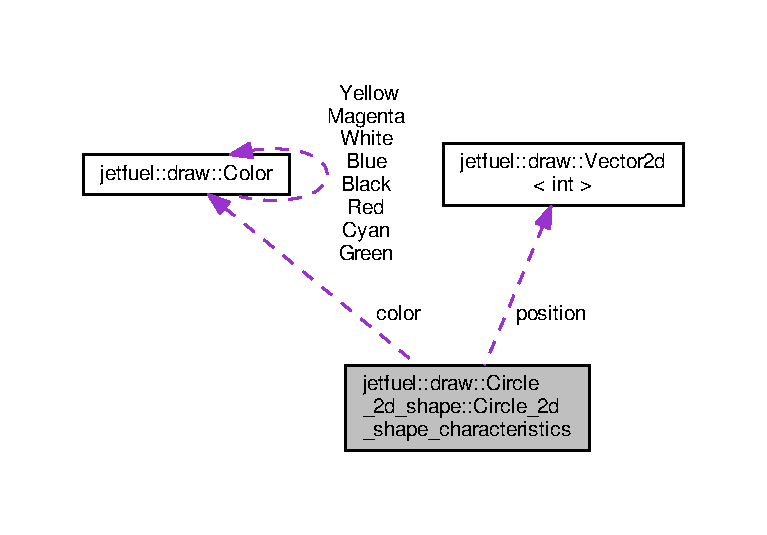
\includegraphics[width=350pt]{structjetfuel_1_1draw_1_1Circle__2d__shape_1_1Circle__2d__shape__characteristics__coll__graph}
\end{center}
\end{figure}
\subsection*{Public Attributes}
\begin{DoxyCompactItemize}
\item 
\mbox{\Hypertarget{structjetfuel_1_1draw_1_1Circle__2d__shape_1_1Circle__2d__shape__characteristics_a803262245b8b2213ef89ccb5b4924a81}\label{structjetfuel_1_1draw_1_1Circle__2d__shape_1_1Circle__2d__shape__characteristics_a803262245b8b2213ef89ccb5b4924a81}} 
\hyperlink{classjetfuel_1_1draw_1_1Vector2d}{Vector2d\+\_\+int} {\bfseries position}
\item 
\mbox{\Hypertarget{structjetfuel_1_1draw_1_1Circle__2d__shape_1_1Circle__2d__shape__characteristics_a6f14b4f3bb802098bc0f2833d26253ae}\label{structjetfuel_1_1draw_1_1Circle__2d__shape_1_1Circle__2d__shape__characteristics_a6f14b4f3bb802098bc0f2833d26253ae}} 
int {\bfseries radius} = 0
\item 
\mbox{\Hypertarget{structjetfuel_1_1draw_1_1Circle__2d__shape_1_1Circle__2d__shape__characteristics_a852915bdc0361e5d7bd4b21b66bcee72}\label{structjetfuel_1_1draw_1_1Circle__2d__shape_1_1Circle__2d__shape__characteristics_a852915bdc0361e5d7bd4b21b66bcee72}} 
\hyperlink{classjetfuel_1_1draw_1_1Color}{Color} {\bfseries color}
\item 
\mbox{\Hypertarget{structjetfuel_1_1draw_1_1Circle__2d__shape_1_1Circle__2d__shape__characteristics_a5ff35e007125e6f0ed97dcc43532a756}\label{structjetfuel_1_1draw_1_1Circle__2d__shape_1_1Circle__2d__shape__characteristics_a5ff35e007125e6f0ed97dcc43532a756}} 
bool {\bfseries antialiasingstatus} = false
\item 
\mbox{\Hypertarget{structjetfuel_1_1draw_1_1Circle__2d__shape_1_1Circle__2d__shape__characteristics_ae4f99c0c5abaa938d89e87aa4d70a6b4}\label{structjetfuel_1_1draw_1_1Circle__2d__shape_1_1Circle__2d__shape__characteristics_ae4f99c0c5abaa938d89e87aa4d70a6b4}} 
bool {\bfseries filledcirclestatus} = false
\end{DoxyCompactItemize}


The documentation for this struct was generated from the following file\+:\begin{DoxyCompactItemize}
\item 
include/jetfueldraw/circle2dshape.\+h\end{DoxyCompactItemize}

\hypertarget{classjetfuel_1_1draw_1_1Circle__interface}{}\section{jetfuel\+:\+:draw\+:\+:Circle\+\_\+interface Class Reference}
\label{classjetfuel_1_1draw_1_1Circle__interface}\index{jetfuel\+::draw\+::\+Circle\+\_\+interface@{jetfuel\+::draw\+::\+Circle\+\_\+interface}}


{\ttfamily \#include $<$circleinterface.\+h$>$}



Inheritance diagram for jetfuel\+:\+:draw\+:\+:Circle\+\_\+interface\+:\nopagebreak
\begin{figure}[H]
\begin{center}
\leavevmode
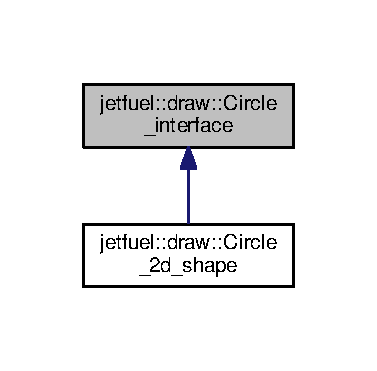
\includegraphics[width=181pt]{classjetfuel_1_1draw_1_1Circle__interface__inherit__graph}
\end{center}
\end{figure}
\subsection*{Public Member Functions}
\begin{DoxyCompactItemize}
\item 
virtual \hyperlink{classjetfuel_1_1draw_1_1Circle2d}{Circle2d\+\_\+int} \hyperlink{classjetfuel_1_1draw_1_1Circle__interface_a992a93bc130288ec4c9c4d2fa4203341}{Get\+\_\+circle\+\_\+to\+\_\+draw} ()=0
\begin{DoxyCompactList}\small\item\em Gets the circle that will be drawn. \end{DoxyCompactList}\end{DoxyCompactItemize}


\subsection{Detailed Description}
A simple interface that specifies unique functions \hyperlink{classjetfuel_1_1draw_1_1Drawable}{Drawable} circles should implement.

\begin{DoxySeeAlso}{See also}
\hyperlink{classjetfuel_1_1draw_1_1Circle__2d__shape}{jetfuel\+::draw\+::\+Circle\+\_\+2d\+\_\+shape} 
\end{DoxySeeAlso}


\subsection{Member Function Documentation}
\mbox{\Hypertarget{classjetfuel_1_1draw_1_1Circle__interface_a992a93bc130288ec4c9c4d2fa4203341}\label{classjetfuel_1_1draw_1_1Circle__interface_a992a93bc130288ec4c9c4d2fa4203341}} 
\index{jetfuel\+::draw\+::\+Circle\+\_\+interface@{jetfuel\+::draw\+::\+Circle\+\_\+interface}!Get\+\_\+circle\+\_\+to\+\_\+draw@{Get\+\_\+circle\+\_\+to\+\_\+draw}}
\index{Get\+\_\+circle\+\_\+to\+\_\+draw@{Get\+\_\+circle\+\_\+to\+\_\+draw}!jetfuel\+::draw\+::\+Circle\+\_\+interface@{jetfuel\+::draw\+::\+Circle\+\_\+interface}}
\subsubsection{\texorpdfstring{Get\+\_\+circle\+\_\+to\+\_\+draw()}{Get\_circle\_to\_draw()}}
{\footnotesize\ttfamily virtual \hyperlink{classjetfuel_1_1draw_1_1Circle2d}{Circle2d\+\_\+int} jetfuel\+::draw\+::\+Circle\+\_\+interface\+::\+Get\+\_\+circle\+\_\+to\+\_\+draw (\begin{DoxyParamCaption}{ }\end{DoxyParamCaption})\hspace{0.3cm}{\ttfamily [pure virtual]}}



Gets the circle that will be drawn. 

This is a pure virtual function (that should get the circle that will be drawn) that must be implemented by any class that inherits this class. 

Implemented in \hyperlink{classjetfuel_1_1draw_1_1Circle__2d__shape_ab188ed6716dff22d0498a01ac1e93d90}{jetfuel\+::draw\+::\+Circle\+\_\+2d\+\_\+shape}.



The documentation for this class was generated from the following file\+:\begin{DoxyCompactItemize}
\item 
include/jetfueldraw/circleinterface.\+h\end{DoxyCompactItemize}

\hypertarget{classjetfuel_1_1draw_1_1Color}{}\section{jetfuel\+:\+:draw\+:\+:Color Class Reference}
\label{classjetfuel_1_1draw_1_1Color}\index{jetfuel\+::draw\+::\+Color@{jetfuel\+::draw\+::\+Color}}


{\ttfamily \#include $<$color.\+h$>$}



Collaboration diagram for jetfuel\+:\+:draw\+:\+:Color\+:
\nopagebreak
\begin{figure}[H]
\begin{center}
\leavevmode
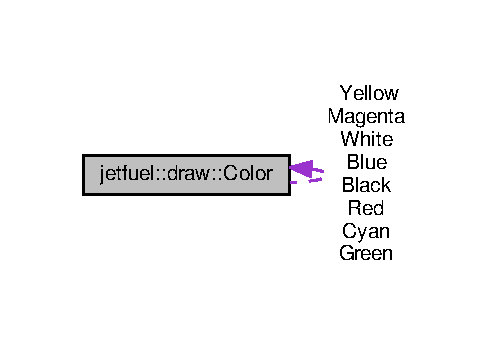
\includegraphics[width=235pt]{classjetfuel_1_1draw_1_1Color__coll__graph}
\end{center}
\end{figure}
\subsection*{Public Member Functions}
\begin{DoxyCompactItemize}
\item 
\hyperlink{classjetfuel_1_1draw_1_1Color_a0deb50ab0c45f96bf039d595fda8d6c3}{Color} ()
\begin{DoxyCompactList}\small\item\em Default Constructor. \end{DoxyCompactList}\item 
\hyperlink{classjetfuel_1_1draw_1_1Color_a4fadffbafbdae0386fc71cf7626dc988}{Color} (unsigned int red, unsigned int green, unsigned int blue, unsigned int alpha=255)
\begin{DoxyCompactList}\small\item\em Construct a color from R\+G\+BA values. \end{DoxyCompactList}\end{DoxyCompactItemize}
\subsection*{Public Attributes}
\begin{DoxyCompactItemize}
\item 
unsigned int \hyperlink{classjetfuel_1_1draw_1_1Color_a282cc70a95a42570a350d2de16376346}{r}
\begin{DoxyCompactList}\small\item\em Member data ///. \end{DoxyCompactList}\item 
\mbox{\Hypertarget{classjetfuel_1_1draw_1_1Color_a5229cd76a67a7236ad54ee2335c1c98a}\label{classjetfuel_1_1draw_1_1Color_a5229cd76a67a7236ad54ee2335c1c98a}} 
unsigned int \hyperlink{classjetfuel_1_1draw_1_1Color_a5229cd76a67a7236ad54ee2335c1c98a}{g}
\begin{DoxyCompactList}\small\item\em Green value. \end{DoxyCompactList}\item 
\mbox{\Hypertarget{classjetfuel_1_1draw_1_1Color_af4152e984d80c8486184be7572783ebf}\label{classjetfuel_1_1draw_1_1Color_af4152e984d80c8486184be7572783ebf}} 
unsigned int \hyperlink{classjetfuel_1_1draw_1_1Color_af4152e984d80c8486184be7572783ebf}{b}
\begin{DoxyCompactList}\small\item\em Blue value. \end{DoxyCompactList}\item 
\mbox{\Hypertarget{classjetfuel_1_1draw_1_1Color_a5155fa4fb77a1e8058c79345de5300c4}\label{classjetfuel_1_1draw_1_1Color_a5155fa4fb77a1e8058c79345de5300c4}} 
unsigned int \hyperlink{classjetfuel_1_1draw_1_1Color_a5155fa4fb77a1e8058c79345de5300c4}{a}
\begin{DoxyCompactList}\small\item\em Alpha (transparency) value. \end{DoxyCompactList}\end{DoxyCompactItemize}
\subsection*{Static Public Attributes}
\begin{DoxyCompactItemize}
\item 
static const \hyperlink{classjetfuel_1_1draw_1_1Color}{Color} \hyperlink{classjetfuel_1_1draw_1_1Color_af7ba2fe7adb5154cde6f5563c5582988}{Black}
\begin{DoxyCompactList}\small\item\em Predefined color presets ///. \end{DoxyCompactList}\item 
\mbox{\Hypertarget{classjetfuel_1_1draw_1_1Color_ab75797c1cb6e4dd952037916db39b5e8}\label{classjetfuel_1_1draw_1_1Color_ab75797c1cb6e4dd952037916db39b5e8}} 
static const \hyperlink{classjetfuel_1_1draw_1_1Color}{Color} \hyperlink{classjetfuel_1_1draw_1_1Color_ab75797c1cb6e4dd952037916db39b5e8}{White}
\begin{DoxyCompactList}\small\item\em White predefined color. \end{DoxyCompactList}\item 
\mbox{\Hypertarget{classjetfuel_1_1draw_1_1Color_a17b1ca508090fecb06707af5bd5e20fb}\label{classjetfuel_1_1draw_1_1Color_a17b1ca508090fecb06707af5bd5e20fb}} 
static const \hyperlink{classjetfuel_1_1draw_1_1Color}{Color} \hyperlink{classjetfuel_1_1draw_1_1Color_a17b1ca508090fecb06707af5bd5e20fb}{Red}
\begin{DoxyCompactList}\small\item\em Red predefined color. \end{DoxyCompactList}\item 
\mbox{\Hypertarget{classjetfuel_1_1draw_1_1Color_a529fbdf4a2a9915e3986278715a5daa8}\label{classjetfuel_1_1draw_1_1Color_a529fbdf4a2a9915e3986278715a5daa8}} 
static const \hyperlink{classjetfuel_1_1draw_1_1Color}{Color} \hyperlink{classjetfuel_1_1draw_1_1Color_a529fbdf4a2a9915e3986278715a5daa8}{Green}
\begin{DoxyCompactList}\small\item\em Green predefined color. \end{DoxyCompactList}\item 
\mbox{\Hypertarget{classjetfuel_1_1draw_1_1Color_a6a9b5ba6b4999d1659b7186fa239f249}\label{classjetfuel_1_1draw_1_1Color_a6a9b5ba6b4999d1659b7186fa239f249}} 
static const \hyperlink{classjetfuel_1_1draw_1_1Color}{Color} \hyperlink{classjetfuel_1_1draw_1_1Color_a6a9b5ba6b4999d1659b7186fa239f249}{Blue}
\begin{DoxyCompactList}\small\item\em Blue predefined color. \end{DoxyCompactList}\item 
\mbox{\Hypertarget{classjetfuel_1_1draw_1_1Color_ac6bc331292535b3d3a3ed51be5832e51}\label{classjetfuel_1_1draw_1_1Color_ac6bc331292535b3d3a3ed51be5832e51}} 
static const \hyperlink{classjetfuel_1_1draw_1_1Color}{Color} \hyperlink{classjetfuel_1_1draw_1_1Color_ac6bc331292535b3d3a3ed51be5832e51}{Yellow}
\begin{DoxyCompactList}\small\item\em Yellow predefined color. \end{DoxyCompactList}\item 
\mbox{\Hypertarget{classjetfuel_1_1draw_1_1Color_a4382e35bf37821db21480378fd6e9c6d}\label{classjetfuel_1_1draw_1_1Color_a4382e35bf37821db21480378fd6e9c6d}} 
static const \hyperlink{classjetfuel_1_1draw_1_1Color}{Color} \hyperlink{classjetfuel_1_1draw_1_1Color_a4382e35bf37821db21480378fd6e9c6d}{Magenta}
\begin{DoxyCompactList}\small\item\em Magenta predefined color. \end{DoxyCompactList}\item 
\mbox{\Hypertarget{classjetfuel_1_1draw_1_1Color_a9c9781b9377310494e8af2a5fe524ab4}\label{classjetfuel_1_1draw_1_1Color_a9c9781b9377310494e8af2a5fe524ab4}} 
static const \hyperlink{classjetfuel_1_1draw_1_1Color}{Color} \hyperlink{classjetfuel_1_1draw_1_1Color_a9c9781b9377310494e8af2a5fe524ab4}{Cyan}
\begin{DoxyCompactList}\small\item\em Cyan predefined color. \end{DoxyCompactList}\end{DoxyCompactItemize}
\subsection*{Related Functions}
(Note that these are not member functions.) \begin{DoxyCompactItemize}
\item 
\hyperlink{classjetfuel_1_1draw_1_1Color}{Color} \hyperlink{classjetfuel_1_1draw_1_1Color_ab6396e36884cc40f26e35f2ef17ce38b}{operator+} (const \hyperlink{classjetfuel_1_1draw_1_1Color}{Color} left, const \hyperlink{classjetfuel_1_1draw_1_1Color}{Color} right)
\begin{DoxyCompactList}\small\item\em Overload of the + operator. \end{DoxyCompactList}\item 
\hyperlink{classjetfuel_1_1draw_1_1Color}{Color} \hyperlink{classjetfuel_1_1draw_1_1Color_aa6992ba7435232c7cd36cce08531f343}{operator-\/} (const \hyperlink{classjetfuel_1_1draw_1_1Color}{Color} left, const \hyperlink{classjetfuel_1_1draw_1_1Color}{Color} right)
\begin{DoxyCompactList}\small\item\em Overload of the -\/ operator. \end{DoxyCompactList}\item 
\hyperlink{classjetfuel_1_1draw_1_1Color}{Color} \hyperlink{classjetfuel_1_1draw_1_1Color_a226f4b8ca4054f4cb338e7c33bbc71c5}{operator+=} (\hyperlink{classjetfuel_1_1draw_1_1Color}{Color} left, \hyperlink{classjetfuel_1_1draw_1_1Color}{Color} right)
\begin{DoxyCompactList}\small\item\em Overload of the += operator. \end{DoxyCompactList}\item 
\hyperlink{classjetfuel_1_1draw_1_1Color}{Color} \hyperlink{classjetfuel_1_1draw_1_1Color_aad218c71ae58d4895e18fb6cd109d91f}{operator-\/=} (\hyperlink{classjetfuel_1_1draw_1_1Color}{Color} left, \hyperlink{classjetfuel_1_1draw_1_1Color}{Color} right)
\begin{DoxyCompactList}\small\item\em Overload of the -\/= operator. \end{DoxyCompactList}\end{DoxyCompactItemize}


\subsection{Detailed Description}
A simple useful class for working with rgba colors. This can be used with the Rectangle2dshape object or with the \hyperlink{classjetfuel_1_1draw_1_1Text}{Text} object.

Code Example\+: \hyperlink{classjetfuel_1_1draw_1_1Scene__manager}{jetfuel\+::draw\+::\+Scene\+\_\+manager} scenemanager; \hyperlink{classjetfuel_1_1draw_1_1Scene}{jetfuel\+::draw\+::\+Scene} scene1(1); \hyperlink{classjetfuel_1_1draw_1_1Color}{jetfuel\+::draw\+::\+Color} color(jetfuel\+::draw\+::\+Color\+::\+Blue); \hyperlink{classjetfuel_1_1draw_1_1Rectangle__2d__shape}{jetfuel\+::draw\+::\+Rectangle\+\_\+2d\+\_\+shape} rectangle( jetfuel\+::draw\+::\+Rect2d\+\_\+int(50,50,50,100);

if(!scenemanager.Create\+\_\+window(\char`\"{}example\char`\"{}, jetfuel\+::draw\+::\+Vector2d\+\_\+int(0,0), jetfuel\+::draw\+::\+Vector2d\+\_\+int(500,500)))\{ std\+::cerr $<$$<$ \char`\"{}\mbox{[}!\mbox{]}\+E\+R\+R\+O\+R with creating sdl renderer!\char`\"{} $<$$<$ \char`\"{}\+Error is\+:\char`\"{} $<$$<$ S\+D\+L\+\_\+\+Get\+Error() $<$$<$ \char`\"{}\textbackslash{}n\char`\"{}; \}

if(!scenemanager.Create\+\_\+renderer())\{ std\+::cerr $<$$<$ \char`\"{}\mbox{[}!\mbox{]}\+E\+R\+R\+O\+R with creating sdl renderer!\char`\"{} $<$$<$ \char`\"{}\+Error is\+:\char`\"{} $<$$<$ S\+D\+L\+\_\+\+Get\+Error() $<$$<$ \char`\"{}\textbackslash{}n\char`\"{}; \}

scenemanager.\+Switch\+\_\+current\+\_\+scene(\&scene1); scene1.\+Attach\+\_\+drawable(\&background); rectangle.\+Set\+\_\+fill\+\_\+color(color);

scenemanager.\+Draw\+\_\+current\+\_\+scene(); 

\subsection{Constructor \& Destructor Documentation}
\mbox{\Hypertarget{classjetfuel_1_1draw_1_1Color_a0deb50ab0c45f96bf039d595fda8d6c3}\label{classjetfuel_1_1draw_1_1Color_a0deb50ab0c45f96bf039d595fda8d6c3}} 
\index{jetfuel\+::draw\+::\+Color@{jetfuel\+::draw\+::\+Color}!Color@{Color}}
\index{Color@{Color}!jetfuel\+::draw\+::\+Color@{jetfuel\+::draw\+::\+Color}}
\subsubsection{\texorpdfstring{Color()}{Color()}\hspace{0.1cm}{\footnotesize\ttfamily [1/2]}}
{\footnotesize\ttfamily jetfuel\+::draw\+::\+Color\+::\+Color (\begin{DoxyParamCaption}{ }\end{DoxyParamCaption})}



Default Constructor. 

Constructs a default color of black with it\textquotesingle{}s transparency(alpha) variable set to 255. \mbox{\Hypertarget{classjetfuel_1_1draw_1_1Color_a4fadffbafbdae0386fc71cf7626dc988}\label{classjetfuel_1_1draw_1_1Color_a4fadffbafbdae0386fc71cf7626dc988}} 
\index{jetfuel\+::draw\+::\+Color@{jetfuel\+::draw\+::\+Color}!Color@{Color}}
\index{Color@{Color}!jetfuel\+::draw\+::\+Color@{jetfuel\+::draw\+::\+Color}}
\subsubsection{\texorpdfstring{Color()}{Color()}\hspace{0.1cm}{\footnotesize\ttfamily [2/2]}}
{\footnotesize\ttfamily jetfuel\+::draw\+::\+Color\+::\+Color (\begin{DoxyParamCaption}\item[{unsigned int}]{red,  }\item[{unsigned int}]{green,  }\item[{unsigned int}]{blue,  }\item[{unsigned int}]{alpha = {\ttfamily 255} }\end{DoxyParamCaption})}



Construct a color from R\+G\+BA values. 

Construct a \hyperlink{classjetfuel_1_1draw_1_1Color}{Color} from the red, green, blue, and alpha(255 if none is specified) values.


\begin{DoxyParams}{Parameters}
{\em unsigned} & int red \\
\hline
{\em unsigned} & int green \\
\hline
{\em unsigned} & int blue \\
\hline
{\em unsigned} & int alpha \\
\hline
\end{DoxyParams}


\subsection{Friends And Related Function Documentation}
\mbox{\Hypertarget{classjetfuel_1_1draw_1_1Color_ab6396e36884cc40f26e35f2ef17ce38b}\label{classjetfuel_1_1draw_1_1Color_ab6396e36884cc40f26e35f2ef17ce38b}} 
\index{jetfuel\+::draw\+::\+Color@{jetfuel\+::draw\+::\+Color}!operator+@{operator+}}
\index{operator+@{operator+}!jetfuel\+::draw\+::\+Color@{jetfuel\+::draw\+::\+Color}}
\subsubsection{\texorpdfstring{operator+()}{operator+()}}
{\footnotesize\ttfamily \hyperlink{classjetfuel_1_1draw_1_1Color}{Color} operator+ (\begin{DoxyParamCaption}\item[{const \hyperlink{classjetfuel_1_1draw_1_1Color}{Color}}]{left,  }\item[{const \hyperlink{classjetfuel_1_1draw_1_1Color}{Color}}]{right }\end{DoxyParamCaption})\hspace{0.3cm}{\ttfamily [related]}}



Overload of the + operator. 

This operator adds all the components of 2 colors and returns the result. Components that exceed 255, a limit, will be kept at 255.


\begin{DoxyParams}{Parameters}
{\em \hyperlink{classjetfuel_1_1draw_1_1Color}{Color}} & left \\
\hline
{\em \hyperlink{classjetfuel_1_1draw_1_1Color}{Color}} & right \\
\hline
\end{DoxyParams}
\mbox{\Hypertarget{classjetfuel_1_1draw_1_1Color_a226f4b8ca4054f4cb338e7c33bbc71c5}\label{classjetfuel_1_1draw_1_1Color_a226f4b8ca4054f4cb338e7c33bbc71c5}} 
\index{jetfuel\+::draw\+::\+Color@{jetfuel\+::draw\+::\+Color}!operator+=@{operator+=}}
\index{operator+=@{operator+=}!jetfuel\+::draw\+::\+Color@{jetfuel\+::draw\+::\+Color}}
\subsubsection{\texorpdfstring{operator+=()}{operator+=()}}
{\footnotesize\ttfamily \hyperlink{classjetfuel_1_1draw_1_1Color}{Color} operator+= (\begin{DoxyParamCaption}\item[{\hyperlink{classjetfuel_1_1draw_1_1Color}{Color}}]{left,  }\item[{\hyperlink{classjetfuel_1_1draw_1_1Color}{Color}}]{right }\end{DoxyParamCaption})\hspace{0.3cm}{\ttfamily [related]}}



Overload of the += operator. 

This operator adds all the components of 2 colors and assigns the result to the left operand. Components that exceed 255, a limit, will be kept at 255.


\begin{DoxyParams}{Parameters}
{\em \hyperlink{classjetfuel_1_1draw_1_1Color}{Color}} & left \\
\hline
{\em \hyperlink{classjetfuel_1_1draw_1_1Color}{Color}} & right \\
\hline
\end{DoxyParams}
\mbox{\Hypertarget{classjetfuel_1_1draw_1_1Color_aa6992ba7435232c7cd36cce08531f343}\label{classjetfuel_1_1draw_1_1Color_aa6992ba7435232c7cd36cce08531f343}} 
\index{jetfuel\+::draw\+::\+Color@{jetfuel\+::draw\+::\+Color}!operator-\/@{operator-\/}}
\index{operator-\/@{operator-\/}!jetfuel\+::draw\+::\+Color@{jetfuel\+::draw\+::\+Color}}
\subsubsection{\texorpdfstring{operator-\/()}{operator-()}}
{\footnotesize\ttfamily \hyperlink{classjetfuel_1_1draw_1_1Color}{Color} operator-\/ (\begin{DoxyParamCaption}\item[{const \hyperlink{classjetfuel_1_1draw_1_1Color}{Color}}]{left,  }\item[{const \hyperlink{classjetfuel_1_1draw_1_1Color}{Color}}]{right }\end{DoxyParamCaption})\hspace{0.3cm}{\ttfamily [related]}}



Overload of the -\/ operator. 

This operator subtracts all the components of 2 colors and returns the result. Components that are below 0, a limit, will be kept at 0.


\begin{DoxyParams}{Parameters}
{\em \hyperlink{classjetfuel_1_1draw_1_1Color}{Color}} & left \\
\hline
{\em \hyperlink{classjetfuel_1_1draw_1_1Color}{Color}} & right \\
\hline
\end{DoxyParams}
\mbox{\Hypertarget{classjetfuel_1_1draw_1_1Color_aad218c71ae58d4895e18fb6cd109d91f}\label{classjetfuel_1_1draw_1_1Color_aad218c71ae58d4895e18fb6cd109d91f}} 
\index{jetfuel\+::draw\+::\+Color@{jetfuel\+::draw\+::\+Color}!operator-\/=@{operator-\/=}}
\index{operator-\/=@{operator-\/=}!jetfuel\+::draw\+::\+Color@{jetfuel\+::draw\+::\+Color}}
\subsubsection{\texorpdfstring{operator-\/=()}{operator-=()}}
{\footnotesize\ttfamily \hyperlink{classjetfuel_1_1draw_1_1Color}{Color} operator-\/= (\begin{DoxyParamCaption}\item[{\hyperlink{classjetfuel_1_1draw_1_1Color}{Color}}]{left,  }\item[{\hyperlink{classjetfuel_1_1draw_1_1Color}{Color}}]{right }\end{DoxyParamCaption})\hspace{0.3cm}{\ttfamily [related]}}



Overload of the -\/= operator. 

This operator subtracts all the components of 2 colors and assigns the result to the left operand. Components that are below 0, a limit, will be kept at 0.


\begin{DoxyParams}{Parameters}
{\em \hyperlink{classjetfuel_1_1draw_1_1Color}{Color}} & left \\
\hline
{\em \hyperlink{classjetfuel_1_1draw_1_1Color}{Color}} & right \\
\hline
\end{DoxyParams}


\subsection{Member Data Documentation}
\mbox{\Hypertarget{classjetfuel_1_1draw_1_1Color_af7ba2fe7adb5154cde6f5563c5582988}\label{classjetfuel_1_1draw_1_1Color_af7ba2fe7adb5154cde6f5563c5582988}} 
\index{jetfuel\+::draw\+::\+Color@{jetfuel\+::draw\+::\+Color}!Black@{Black}}
\index{Black@{Black}!jetfuel\+::draw\+::\+Color@{jetfuel\+::draw\+::\+Color}}
\subsubsection{\texorpdfstring{Black}{Black}}
{\footnotesize\ttfamily const \hyperlink{classjetfuel_1_1draw_1_1Color}{Color} jetfuel\+::draw\+::\+Color\+::\+Black\hspace{0.3cm}{\ttfamily [static]}}



Predefined color presets ///. 

Black predefined color \mbox{\Hypertarget{classjetfuel_1_1draw_1_1Color_a282cc70a95a42570a350d2de16376346}\label{classjetfuel_1_1draw_1_1Color_a282cc70a95a42570a350d2de16376346}} 
\index{jetfuel\+::draw\+::\+Color@{jetfuel\+::draw\+::\+Color}!r@{r}}
\index{r@{r}!jetfuel\+::draw\+::\+Color@{jetfuel\+::draw\+::\+Color}}
\subsubsection{\texorpdfstring{r}{r}}
{\footnotesize\ttfamily unsigned int jetfuel\+::draw\+::\+Color\+::r}



Member data ///. 

Red value 

The documentation for this class was generated from the following file\+:\begin{DoxyCompactItemize}
\item 
include/jetfueldraw/color.\+h\end{DoxyCompactItemize}

\hypertarget{classjetfuel_1_1draw_1_1Drawable}{}\section{jetfuel\+:\+:draw\+:\+:Drawable Class Reference}
\label{classjetfuel_1_1draw_1_1Drawable}\index{jetfuel\+::draw\+::\+Drawable@{jetfuel\+::draw\+::\+Drawable}}


{\ttfamily \#include $<$drawable.\+h$>$}



Inheritance diagram for jetfuel\+:\+:draw\+:\+:Drawable\+:\nopagebreak
\begin{figure}[H]
\begin{center}
\leavevmode
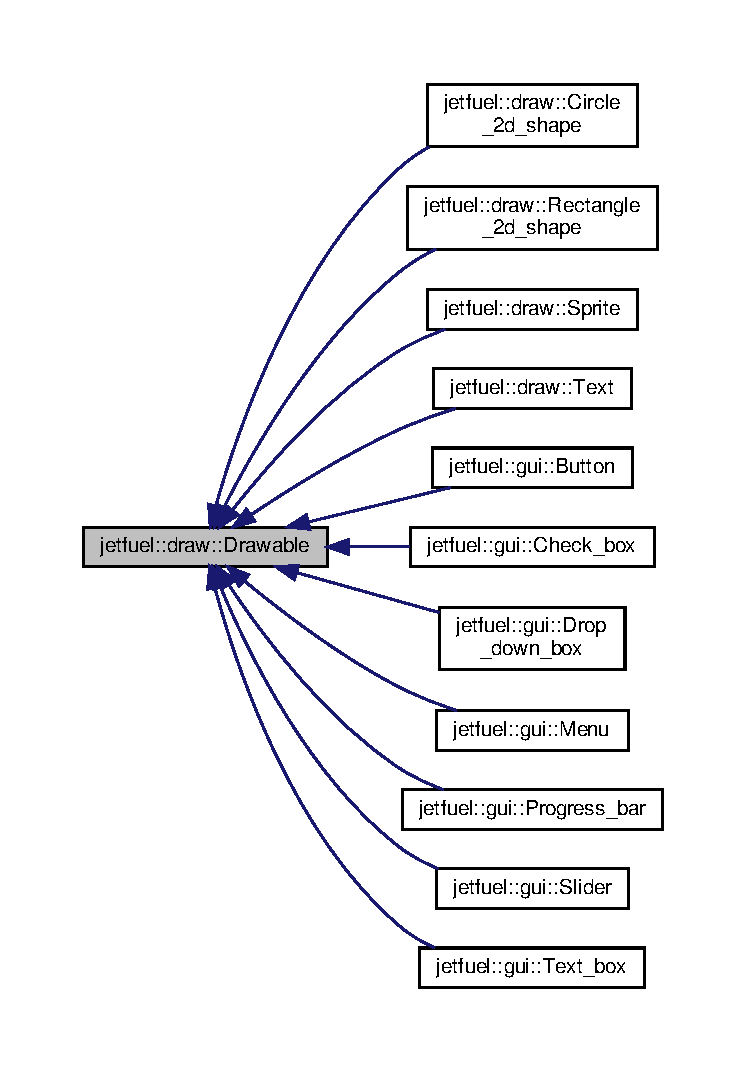
\includegraphics[width=350pt]{classjetfuel_1_1draw_1_1Drawable__inherit__graph}
\end{center}
\end{figure}
\subsection*{Public Member Functions}
\begin{DoxyCompactItemize}
\item 
virtual \hyperlink{classjetfuel_1_1draw_1_1Vector2d}{Vector2d\+\_\+int} \hyperlink{classjetfuel_1_1draw_1_1Drawable_ae7ebd30d66db2c8a5d5371cbcf0023fc}{Get\+\_\+position} ()
\begin{DoxyCompactList}\small\item\em Returns internal m\+\_\+position variable. \end{DoxyCompactList}\item 
virtual void \hyperlink{classjetfuel_1_1draw_1_1Drawable_afdd035afe40c706459a6c9df813bcce6}{Set\+\_\+position} (const \hyperlink{classjetfuel_1_1draw_1_1Vector2d}{Vector2d\+\_\+int} position)
\begin{DoxyCompactList}\small\item\em Set the internal m\+\_\+position variable. \end{DoxyCompactList}\item 
bool \hyperlink{classjetfuel_1_1draw_1_1Drawable_a3b8d50394e8411a8009f50da826b3ac2}{operator==} (\hyperlink{classjetfuel_1_1draw_1_1Drawable}{Drawable} \&drawable)
\begin{DoxyCompactList}\small\item\em Using the \hyperlink{classjetfuel_1_1draw_1_1Drawable}{Drawable}\textquotesingle{}s U\+U\+ID, compare this \hyperlink{classjetfuel_1_1draw_1_1Drawable}{Drawable} with another. \end{DoxyCompactList}\item 
bool \hyperlink{classjetfuel_1_1draw_1_1Drawable_a6def0c6a514cb41cf4791191c06b4c3a}{Assigned\+\_\+renderer} () const
\begin{DoxyCompactList}\small\item\em Returns whether this \hyperlink{classjetfuel_1_1draw_1_1Drawable}{Drawable} was assigned a renderer. \end{DoxyCompactList}\item 
virtual void \hyperlink{classjetfuel_1_1draw_1_1Drawable_a0d7257f197d6ffcdd89c3a99c93d1400}{Assign\+\_\+renderer} (S\+D\+L\+\_\+\+Renderer $\ast$renderer)
\begin{DoxyCompactList}\small\item\em Assigns the renderer to be used by the object. \end{DoxyCompactList}\item 
virtual bool \hyperlink{classjetfuel_1_1draw_1_1Drawable_a1a072070322965ce9411ee6e7c311c56}{Draw} ()=0
\begin{DoxyCompactList}\small\item\em Draws the object. \end{DoxyCompactList}\end{DoxyCompactItemize}
\subsection*{Protected Member Functions}
\begin{DoxyCompactItemize}
\item 
S\+D\+L\+\_\+\+Rect \hyperlink{classjetfuel_1_1draw_1_1Drawable_a8709fde1dc750d3c6ca5ecb8b9b4fb12}{Get\+\_\+dest} () const
\begin{DoxyCompactList}\small\item\em Gets the internal destination S\+D\+L\+\_\+\+Rect variable. \end{DoxyCompactList}\item 
void \hyperlink{classjetfuel_1_1draw_1_1Drawable_a75a4f944021825be72d3d7f3da7e1093}{Set\+\_\+dest} (const S\+D\+L\+\_\+\+Rect dest)
\begin{DoxyCompactList}\small\item\em Sets the internal destination S\+D\+L\+\_\+\+Rect variable. \end{DoxyCompactList}\item 
void \hyperlink{classjetfuel_1_1draw_1_1Drawable_af8ff41fd1f3e2787743f916386ea225c}{Set\+\_\+assigned\+\_\+renderer} (bool rendererassigned)
\begin{DoxyCompactList}\small\item\em Sets the variable that tells whether the renderer was assigned or not. \end{DoxyCompactList}\item 
virtual S\+D\+L\+\_\+\+Renderer $\ast$ \hyperlink{classjetfuel_1_1draw_1_1Drawable_a6bbda81a7fbd33c388039ecaeb53c278}{Get\+\_\+renderer} ()
\begin{DoxyCompactList}\small\item\em Gets the renderer to be used for drawing. \end{DoxyCompactList}\end{DoxyCompactItemize}


\subsection{Detailed Description}
A simple header-\/only base class that provides a base if you want to make a sprite that uses the renderer.

You must inherit from this class if you want to draw it to the screen via \hyperlink{classjetfuel_1_1draw_1_1Scene}{jetfuel\+::draw\+::\+Scene}.

\begin{DoxySeeAlso}{See also}
\hyperlink{classjetfuel_1_1draw_1_1Sprite}{jetfuel\+::draw\+::\+Sprite} 

\hyperlink{classjetfuel_1_1draw_1_1Text}{jetfuel\+::draw\+::\+Text} 

\hyperlink{classjetfuel_1_1draw_1_1Rectangle__2d__shape}{jetfuel\+::draw\+::\+Rectangle\+\_\+2d\+\_\+shape} 
\end{DoxySeeAlso}


\subsection{Member Function Documentation}
\mbox{\Hypertarget{classjetfuel_1_1draw_1_1Drawable_a0d7257f197d6ffcdd89c3a99c93d1400}\label{classjetfuel_1_1draw_1_1Drawable_a0d7257f197d6ffcdd89c3a99c93d1400}} 
\index{jetfuel\+::draw\+::\+Drawable@{jetfuel\+::draw\+::\+Drawable}!Assign\+\_\+renderer@{Assign\+\_\+renderer}}
\index{Assign\+\_\+renderer@{Assign\+\_\+renderer}!jetfuel\+::draw\+::\+Drawable@{jetfuel\+::draw\+::\+Drawable}}
\subsubsection{\texorpdfstring{Assign\+\_\+renderer()}{Assign\_renderer()}}
{\footnotesize\ttfamily virtual void jetfuel\+::draw\+::\+Drawable\+::\+Assign\+\_\+renderer (\begin{DoxyParamCaption}\item[{S\+D\+L\+\_\+\+Renderer $\ast$}]{renderer }\end{DoxyParamCaption})\hspace{0.3cm}{\ttfamily [inline]}, {\ttfamily [virtual]}}



Assigns the renderer to be used by the object. 

Assigns the renderer to be used by the object while drawing.

This function should only be used by the \hyperlink{classjetfuel_1_1draw_1_1Scene__manager}{Scene\+\_\+manager} if you are using the \hyperlink{classjetfuel_1_1draw_1_1Scene__manager}{Scene\+\_\+manager} and \hyperlink{classjetfuel_1_1draw_1_1Scene}{Scene} objects.


\begin{DoxyParams}{Parameters}
{\em S\+D\+L\+\_\+\+Renderer} & $\ast$renderer \\
\hline
\end{DoxyParams}


Reimplemented in \hyperlink{classjetfuel_1_1gui_1_1Button_aa566a1d59623fde8d062c3d02b6fd5f4}{jetfuel\+::gui\+::\+Button}, \hyperlink{classjetfuel_1_1gui_1_1Menu_acf4a69ccd0ee1490d02fa005c8eba1b4}{jetfuel\+::gui\+::\+Menu}, \hyperlink{classjetfuel_1_1gui_1_1Slider_af9ceba04fec0f7cdc097ea0513094176}{jetfuel\+::gui\+::\+Slider}, \hyperlink{classjetfuel_1_1gui_1_1Drop__down__box_a9160249744bdd278e20a77f470421d3e}{jetfuel\+::gui\+::\+Drop\+\_\+down\+\_\+box}, \hyperlink{classjetfuel_1_1gui_1_1Progress__bar_a34797d42cedf5ff096eafb58c2e76128}{jetfuel\+::gui\+::\+Progress\+\_\+bar}, and \hyperlink{classjetfuel_1_1gui_1_1Check__box_a544261fc2f2d182b73c7ea629fa35e78}{jetfuel\+::gui\+::\+Check\+\_\+box}.

\mbox{\Hypertarget{classjetfuel_1_1draw_1_1Drawable_a6def0c6a514cb41cf4791191c06b4c3a}\label{classjetfuel_1_1draw_1_1Drawable_a6def0c6a514cb41cf4791191c06b4c3a}} 
\index{jetfuel\+::draw\+::\+Drawable@{jetfuel\+::draw\+::\+Drawable}!Assigned\+\_\+renderer@{Assigned\+\_\+renderer}}
\index{Assigned\+\_\+renderer@{Assigned\+\_\+renderer}!jetfuel\+::draw\+::\+Drawable@{jetfuel\+::draw\+::\+Drawable}}
\subsubsection{\texorpdfstring{Assigned\+\_\+renderer()}{Assigned\_renderer()}}
{\footnotesize\ttfamily bool jetfuel\+::draw\+::\+Drawable\+::\+Assigned\+\_\+renderer (\begin{DoxyParamCaption}{ }\end{DoxyParamCaption}) const\hspace{0.3cm}{\ttfamily [inline]}}



Returns whether this \hyperlink{classjetfuel_1_1draw_1_1Drawable}{Drawable} was assigned a renderer. 

Returns whether this \hyperlink{classjetfuel_1_1draw_1_1Drawable}{Drawable} was assigned a renderer based on a internal private boolean variable set to true when the function Assign\+\_\+renderer has been called and false otherwise. \mbox{\Hypertarget{classjetfuel_1_1draw_1_1Drawable_a1a072070322965ce9411ee6e7c311c56}\label{classjetfuel_1_1draw_1_1Drawable_a1a072070322965ce9411ee6e7c311c56}} 
\index{jetfuel\+::draw\+::\+Drawable@{jetfuel\+::draw\+::\+Drawable}!Draw@{Draw}}
\index{Draw@{Draw}!jetfuel\+::draw\+::\+Drawable@{jetfuel\+::draw\+::\+Drawable}}
\subsubsection{\texorpdfstring{Draw()}{Draw()}}
{\footnotesize\ttfamily virtual bool jetfuel\+::draw\+::\+Drawable\+::\+Draw (\begin{DoxyParamCaption}{ }\end{DoxyParamCaption})\hspace{0.3cm}{\ttfamily [pure virtual]}}



Draws the object. 

This function (which should draw the object) is a pure virtual one that must be implemented by any class that inherits this class. 

Implemented in \hyperlink{classjetfuel_1_1draw_1_1Text_ac0b8a614277d6b575c52d127e9a673f2}{jetfuel\+::draw\+::\+Text}, \hyperlink{classjetfuel_1_1gui_1_1Menu_a0355f5ee3060b1ae9d85a5c8cba3795b}{jetfuel\+::gui\+::\+Menu}, \hyperlink{classjetfuel_1_1gui_1_1Button_a1c8ec68b90dc461b1603c47fb8c509c4}{jetfuel\+::gui\+::\+Button}, \hyperlink{classjetfuel_1_1gui_1_1Check__box_ad2ce6d4af8d950a4ef76b0688541c29a}{jetfuel\+::gui\+::\+Check\+\_\+box}, \hyperlink{classjetfuel_1_1gui_1_1Slider_a483038c689276ed8468e990977e5a74a}{jetfuel\+::gui\+::\+Slider}, \hyperlink{classjetfuel_1_1gui_1_1Drop__down__box_a1b62cab3674f45700ad9afd6076a8cb1}{jetfuel\+::gui\+::\+Drop\+\_\+down\+\_\+box}, \hyperlink{classjetfuel_1_1gui_1_1Progress__bar_a91a7ffe82738105be9b36a48dca1cdec}{jetfuel\+::gui\+::\+Progress\+\_\+bar}, \hyperlink{classjetfuel_1_1draw_1_1Circle__2d__shape_a8be660f3cd624dc077d9003ee3b37212}{jetfuel\+::draw\+::\+Circle\+\_\+2d\+\_\+shape}, \hyperlink{classjetfuel_1_1draw_1_1Rectangle__2d__shape_aba19e63d55c824de135932483fe40fcb}{jetfuel\+::draw\+::\+Rectangle\+\_\+2d\+\_\+shape}, and \hyperlink{classjetfuel_1_1draw_1_1Sprite_ae4e52cd12a067e67ed67d5a2a5835143}{jetfuel\+::draw\+::\+Sprite}.

\mbox{\Hypertarget{classjetfuel_1_1draw_1_1Drawable_a8709fde1dc750d3c6ca5ecb8b9b4fb12}\label{classjetfuel_1_1draw_1_1Drawable_a8709fde1dc750d3c6ca5ecb8b9b4fb12}} 
\index{jetfuel\+::draw\+::\+Drawable@{jetfuel\+::draw\+::\+Drawable}!Get\+\_\+dest@{Get\+\_\+dest}}
\index{Get\+\_\+dest@{Get\+\_\+dest}!jetfuel\+::draw\+::\+Drawable@{jetfuel\+::draw\+::\+Drawable}}
\subsubsection{\texorpdfstring{Get\+\_\+dest()}{Get\_dest()}}
{\footnotesize\ttfamily S\+D\+L\+\_\+\+Rect jetfuel\+::draw\+::\+Drawable\+::\+Get\+\_\+dest (\begin{DoxyParamCaption}{ }\end{DoxyParamCaption}) const\hspace{0.3cm}{\ttfamily [inline]}, {\ttfamily [protected]}}



Gets the internal destination S\+D\+L\+\_\+\+Rect variable. 

Gets the internal private destination S\+D\+L\+\_\+\+Rect variable to be used when drawing sand positioning a \hyperlink{classjetfuel_1_1draw_1_1Drawable}{Drawable}. \mbox{\Hypertarget{classjetfuel_1_1draw_1_1Drawable_ae7ebd30d66db2c8a5d5371cbcf0023fc}\label{classjetfuel_1_1draw_1_1Drawable_ae7ebd30d66db2c8a5d5371cbcf0023fc}} 
\index{jetfuel\+::draw\+::\+Drawable@{jetfuel\+::draw\+::\+Drawable}!Get\+\_\+position@{Get\+\_\+position}}
\index{Get\+\_\+position@{Get\+\_\+position}!jetfuel\+::draw\+::\+Drawable@{jetfuel\+::draw\+::\+Drawable}}
\subsubsection{\texorpdfstring{Get\+\_\+position()}{Get\_position()}}
{\footnotesize\ttfamily virtual \hyperlink{classjetfuel_1_1draw_1_1Vector2d}{Vector2d\+\_\+int} jetfuel\+::draw\+::\+Drawable\+::\+Get\+\_\+position (\begin{DoxyParamCaption}{ }\end{DoxyParamCaption})\hspace{0.3cm}{\ttfamily [inline]}, {\ttfamily [virtual]}}



Returns internal m\+\_\+position variable. 

Returns private internal m\+\_\+position variable used for positioning. 

Reimplemented in \hyperlink{classjetfuel_1_1gui_1_1Menu_ac1aebb753feba17be808f2068ff17e74}{jetfuel\+::gui\+::\+Menu}, \hyperlink{classjetfuel_1_1gui_1_1Button_aadcceacaabaa40bceb293d1f91231d22}{jetfuel\+::gui\+::\+Button}, \hyperlink{classjetfuel_1_1gui_1_1Slider_a2b177c832a42ad21ca1fa88496ef7551}{jetfuel\+::gui\+::\+Slider}, \hyperlink{classjetfuel_1_1gui_1_1Drop__down__box_af92cccd010b21e1ce64af9a3c58ba086}{jetfuel\+::gui\+::\+Drop\+\_\+down\+\_\+box}, \hyperlink{classjetfuel_1_1gui_1_1Progress__bar_a5771ea71b321c173383e89537cea0ae1}{jetfuel\+::gui\+::\+Progress\+\_\+bar}, \hyperlink{classjetfuel_1_1gui_1_1Check__box_a7f14e8be560d0be5a05839442de1f18f}{jetfuel\+::gui\+::\+Check\+\_\+box}, \hyperlink{classjetfuel_1_1draw_1_1Rectangle__2d__shape_a60aa3e0fa050e3fbd98177c1eef721b0}{jetfuel\+::draw\+::\+Rectangle\+\_\+2d\+\_\+shape}, and \hyperlink{classjetfuel_1_1draw_1_1Circle__2d__shape_a99b93544660c7f5b11cf8f0169e8fec1}{jetfuel\+::draw\+::\+Circle\+\_\+2d\+\_\+shape}.

\mbox{\Hypertarget{classjetfuel_1_1draw_1_1Drawable_a6bbda81a7fbd33c388039ecaeb53c278}\label{classjetfuel_1_1draw_1_1Drawable_a6bbda81a7fbd33c388039ecaeb53c278}} 
\index{jetfuel\+::draw\+::\+Drawable@{jetfuel\+::draw\+::\+Drawable}!Get\+\_\+renderer@{Get\+\_\+renderer}}
\index{Get\+\_\+renderer@{Get\+\_\+renderer}!jetfuel\+::draw\+::\+Drawable@{jetfuel\+::draw\+::\+Drawable}}
\subsubsection{\texorpdfstring{Get\+\_\+renderer()}{Get\_renderer()}}
{\footnotesize\ttfamily virtual S\+D\+L\+\_\+\+Renderer$\ast$ jetfuel\+::draw\+::\+Drawable\+::\+Get\+\_\+renderer (\begin{DoxyParamCaption}{ }\end{DoxyParamCaption})\hspace{0.3cm}{\ttfamily [inline]}, {\ttfamily [protected]}, {\ttfamily [virtual]}}



Gets the renderer to be used for drawing. 

Gets the renderer to be used for drawing purposes. 

Reimplemented in \hyperlink{classjetfuel_1_1gui_1_1Drop__down__box_ab8beac8ed8b442d96723f72a2fe9edb6}{jetfuel\+::gui\+::\+Drop\+\_\+down\+\_\+box}, and \hyperlink{classjetfuel_1_1gui_1_1Menu_a411940386454af4e44dc8c0c84c00215}{jetfuel\+::gui\+::\+Menu}.

\mbox{\Hypertarget{classjetfuel_1_1draw_1_1Drawable_a3b8d50394e8411a8009f50da826b3ac2}\label{classjetfuel_1_1draw_1_1Drawable_a3b8d50394e8411a8009f50da826b3ac2}} 
\index{jetfuel\+::draw\+::\+Drawable@{jetfuel\+::draw\+::\+Drawable}!operator==@{operator==}}
\index{operator==@{operator==}!jetfuel\+::draw\+::\+Drawable@{jetfuel\+::draw\+::\+Drawable}}
\subsubsection{\texorpdfstring{operator==()}{operator==()}}
{\footnotesize\ttfamily bool jetfuel\+::draw\+::\+Drawable\+::operator== (\begin{DoxyParamCaption}\item[{\hyperlink{classjetfuel_1_1draw_1_1Drawable}{Drawable} \&}]{drawable }\end{DoxyParamCaption})\hspace{0.3cm}{\ttfamily [inline]}}



Using the \hyperlink{classjetfuel_1_1draw_1_1Drawable}{Drawable}\textquotesingle{}s U\+U\+ID, compare this \hyperlink{classjetfuel_1_1draw_1_1Drawable}{Drawable} with another. 

Using the \hyperlink{classjetfuel_1_1draw_1_1Drawable}{Drawable}\textquotesingle{}s U\+U\+ID, compare this \hyperlink{classjetfuel_1_1draw_1_1Drawable}{Drawable} with another. The U\+U\+ID ensures that different Drawables with the same exact position and renderer don\textquotesingle{}t get falsely marked as equals.


\begin{DoxyParams}{Parameters}
{\em \hyperlink{classjetfuel_1_1draw_1_1Drawable}{Drawable}} & \&drawable \\
\hline
\end{DoxyParams}
\mbox{\Hypertarget{classjetfuel_1_1draw_1_1Drawable_af8ff41fd1f3e2787743f916386ea225c}\label{classjetfuel_1_1draw_1_1Drawable_af8ff41fd1f3e2787743f916386ea225c}} 
\index{jetfuel\+::draw\+::\+Drawable@{jetfuel\+::draw\+::\+Drawable}!Set\+\_\+assigned\+\_\+renderer@{Set\+\_\+assigned\+\_\+renderer}}
\index{Set\+\_\+assigned\+\_\+renderer@{Set\+\_\+assigned\+\_\+renderer}!jetfuel\+::draw\+::\+Drawable@{jetfuel\+::draw\+::\+Drawable}}
\subsubsection{\texorpdfstring{Set\+\_\+assigned\+\_\+renderer()}{Set\_assigned\_renderer()}}
{\footnotesize\ttfamily void jetfuel\+::draw\+::\+Drawable\+::\+Set\+\_\+assigned\+\_\+renderer (\begin{DoxyParamCaption}\item[{bool}]{rendererassigned }\end{DoxyParamCaption})\hspace{0.3cm}{\ttfamily [inline]}, {\ttfamily [protected]}}



Sets the variable that tells whether the renderer was assigned or not. 

Sets the variable that tells whether the renderer was assigned or not.


\begin{DoxyParams}{Parameters}
{\em bool} & rendererassigned \\
\hline
\end{DoxyParams}
\mbox{\Hypertarget{classjetfuel_1_1draw_1_1Drawable_a75a4f944021825be72d3d7f3da7e1093}\label{classjetfuel_1_1draw_1_1Drawable_a75a4f944021825be72d3d7f3da7e1093}} 
\index{jetfuel\+::draw\+::\+Drawable@{jetfuel\+::draw\+::\+Drawable}!Set\+\_\+dest@{Set\+\_\+dest}}
\index{Set\+\_\+dest@{Set\+\_\+dest}!jetfuel\+::draw\+::\+Drawable@{jetfuel\+::draw\+::\+Drawable}}
\subsubsection{\texorpdfstring{Set\+\_\+dest()}{Set\_dest()}}
{\footnotesize\ttfamily void jetfuel\+::draw\+::\+Drawable\+::\+Set\+\_\+dest (\begin{DoxyParamCaption}\item[{const S\+D\+L\+\_\+\+Rect}]{dest }\end{DoxyParamCaption})\hspace{0.3cm}{\ttfamily [inline]}, {\ttfamily [protected]}}



Sets the internal destination S\+D\+L\+\_\+\+Rect variable. 

Sets the internal private destination S\+D\+L\+\_\+\+Rect variable to be used when drawing and positioning a \hyperlink{classjetfuel_1_1draw_1_1Drawable}{Drawable}.


\begin{DoxyParams}{Parameters}
{\em S\+D\+L\+\_\+\+Rect} & dest \\
\hline
\end{DoxyParams}
\mbox{\Hypertarget{classjetfuel_1_1draw_1_1Drawable_afdd035afe40c706459a6c9df813bcce6}\label{classjetfuel_1_1draw_1_1Drawable_afdd035afe40c706459a6c9df813bcce6}} 
\index{jetfuel\+::draw\+::\+Drawable@{jetfuel\+::draw\+::\+Drawable}!Set\+\_\+position@{Set\+\_\+position}}
\index{Set\+\_\+position@{Set\+\_\+position}!jetfuel\+::draw\+::\+Drawable@{jetfuel\+::draw\+::\+Drawable}}
\subsubsection{\texorpdfstring{Set\+\_\+position()}{Set\_position()}}
{\footnotesize\ttfamily virtual void jetfuel\+::draw\+::\+Drawable\+::\+Set\+\_\+position (\begin{DoxyParamCaption}\item[{const \hyperlink{classjetfuel_1_1draw_1_1Vector2d}{Vector2d\+\_\+int}}]{position }\end{DoxyParamCaption})\hspace{0.3cm}{\ttfamily [inline]}, {\ttfamily [virtual]}}



Set the internal m\+\_\+position variable. 

Set the internal private m\+\_\+position variable used for positioning.


\begin{DoxyParams}{Parameters}
{\em Vector2d\+\_\+int} & position \\
\hline
\end{DoxyParams}


Reimplemented in \hyperlink{classjetfuel_1_1gui_1_1Menu_ab575d5e4ad9d86d6781012e7d1bebc9a}{jetfuel\+::gui\+::\+Menu}, \hyperlink{classjetfuel_1_1gui_1_1Button_a642d3f1412339c826458b80dce76ef34}{jetfuel\+::gui\+::\+Button}, \hyperlink{classjetfuel_1_1gui_1_1Slider_a11721a72699e9d1cdd0f6e5709f003e4}{jetfuel\+::gui\+::\+Slider}, \hyperlink{classjetfuel_1_1gui_1_1Drop__down__box_acba86706261397994c96727a0184a78c}{jetfuel\+::gui\+::\+Drop\+\_\+down\+\_\+box}, \hyperlink{classjetfuel_1_1gui_1_1Progress__bar_a5f52369cccd805274805abf5913535df}{jetfuel\+::gui\+::\+Progress\+\_\+bar}, \hyperlink{classjetfuel_1_1gui_1_1Check__box_aca11db17630485a2c44b19780d10cce6}{jetfuel\+::gui\+::\+Check\+\_\+box}, \hyperlink{classjetfuel_1_1draw_1_1Rectangle__2d__shape_a375b0892589ef7cd1762576e9ce96875}{jetfuel\+::draw\+::\+Rectangle\+\_\+2d\+\_\+shape}, and \hyperlink{classjetfuel_1_1draw_1_1Circle__2d__shape_a551b38063543823483f560bf3eebcd2c}{jetfuel\+::draw\+::\+Circle\+\_\+2d\+\_\+shape}.



The documentation for this class was generated from the following file\+:\begin{DoxyCompactItemize}
\item 
include/jetfueldraw/drawable.\+h\end{DoxyCompactItemize}

\hypertarget{classjetfuel_1_1gui_1_1Drop__down__box}{}\section{jetfuel\+:\+:gui\+:\+:Drop\+\_\+down\+\_\+box Class Reference}
\label{classjetfuel_1_1gui_1_1Drop__down__box}\index{jetfuel\+::gui\+::\+Drop\+\_\+down\+\_\+box@{jetfuel\+::gui\+::\+Drop\+\_\+down\+\_\+box}}


{\ttfamily \#include $<$dropdownbox.\+h$>$}



Inheritance diagram for jetfuel\+:\+:gui\+:\+:Drop\+\_\+down\+\_\+box\+:\nopagebreak
\begin{figure}[H]
\begin{center}
\leavevmode
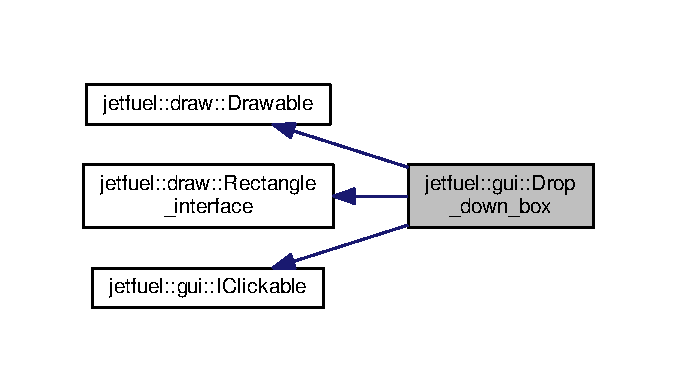
\includegraphics[width=325pt]{classjetfuel_1_1gui_1_1Drop__down__box__inherit__graph}
\end{center}
\end{figure}


Collaboration diagram for jetfuel\+:\+:gui\+:\+:Drop\+\_\+down\+\_\+box\+:\nopagebreak
\begin{figure}[H]
\begin{center}
\leavevmode
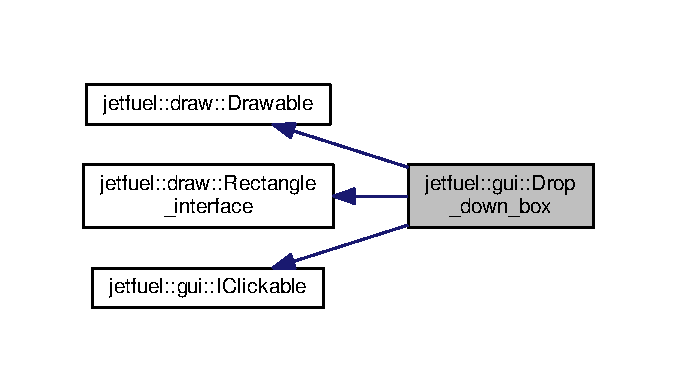
\includegraphics[width=325pt]{classjetfuel_1_1gui_1_1Drop__down__box__coll__graph}
\end{center}
\end{figure}
\subsection*{Classes}
\begin{DoxyCompactItemize}
\item 
struct \hyperlink{structjetfuel_1_1gui_1_1Drop__down__box_1_1Drop__down__option}{Drop\+\_\+down\+\_\+option}
\end{DoxyCompactItemize}
\subsection*{Public Member Functions}
\begin{DoxyCompactItemize}
\item 
\hyperlink{classjetfuel_1_1gui_1_1Drop__down__box_af518d68503aa67f76e70fd4e2d9c3cb3}{Drop\+\_\+down\+\_\+box} ()
\begin{DoxyCompactList}\small\item\em Default constructor. \end{DoxyCompactList}\item 
bool \hyperlink{classjetfuel_1_1gui_1_1Drop__down__box_a9624ef3b9af6d1e3e6fcebb7ef7aa17c}{Load\+\_\+base\+\_\+box\+\_\+image} (\hyperlink{classjetfuel_1_1draw_1_1Image}{jetfuel\+::draw\+::\+Image} baseboximage, const \hyperlink{classjetfuel_1_1draw_1_1Color}{jetfuel\+::draw\+::\+Color} baseboxcolor, const \hyperlink{classjetfuel_1_1draw_1_1Vector2d}{jetfuel\+::draw\+::\+Vector2d\+\_\+uint} bordersizes)
\begin{DoxyCompactList}\small\item\em Loads the base box image of the \hyperlink{classjetfuel_1_1gui_1_1Drop__down__box}{Drop\+\_\+down\+\_\+box}. \end{DoxyCompactList}\item 
void \hyperlink{classjetfuel_1_1gui_1_1Drop__down__box_a64b807d21f55a85ab9600cfd6369d7dc}{Dynamic\+\_\+load\+\_\+base\+\_\+box\+\_\+image} (\hyperlink{classjetfuel_1_1draw_1_1Image}{jetfuel\+::draw\+::\+Image} baseboximage, const \hyperlink{classjetfuel_1_1draw_1_1Color}{jetfuel\+::draw\+::\+Color} baseboxcolor, const \hyperlink{classjetfuel_1_1draw_1_1Vector2d}{jetfuel\+::draw\+::\+Vector2d\+\_\+uint} bordersizes)
\begin{DoxyCompactList}\small\item\em Dynamically loads the base box image of the \hyperlink{classjetfuel_1_1gui_1_1Drop__down__box}{Drop\+\_\+down\+\_\+box}. \end{DoxyCompactList}\item 
std\+::string \hyperlink{classjetfuel_1_1gui_1_1Drop__down__box_ae53f93bddf6764775454246efa7d7e57}{Get\+\_\+active\+\_\+option} () const
\begin{DoxyCompactList}\small\item\em Gets the active option of the \hyperlink{classjetfuel_1_1gui_1_1Drop__down__box}{Drop\+\_\+down\+\_\+box}. \end{DoxyCompactList}\item 
\hyperlink{structjetfuel_1_1draw_1_1Text_1_1Text__characteristics}{jetfuel\+::draw\+::\+Text\+::\+Text\+\_\+characteristics} \hyperlink{classjetfuel_1_1gui_1_1Drop__down__box_a8f8bd91ea279110cab98b78854207ae7}{Get\+\_\+option\+\_\+text\+\_\+characteristics} () const
\begin{DoxyCompactList}\small\item\em Gets the text characteristics of the \hyperlink{classjetfuel_1_1gui_1_1Drop__down__box}{Drop\+\_\+down\+\_\+box}\textquotesingle{}s options. \end{DoxyCompactList}\item 
void \hyperlink{classjetfuel_1_1gui_1_1Drop__down__box_a051d83177f8fa26325dcbdc504ccb0a9}{Set\+\_\+option\+\_\+text\+\_\+characteristics} (\hyperlink{structjetfuel_1_1draw_1_1Text_1_1Text__characteristics}{jetfuel\+::draw\+::\+Text\+::\+Text\+\_\+characteristics} textcharacteristics)
\begin{DoxyCompactList}\small\item\em Sets the text characteristics of the \hyperlink{classjetfuel_1_1gui_1_1Drop__down__box}{Drop\+\_\+down\+\_\+box}\textquotesingle{}s options. \end{DoxyCompactList}\item 
std\+::string \hyperlink{classjetfuel_1_1gui_1_1Drop__down__box_a8de320a3db8d94d9b0846e6ae33e261c}{Get\+\_\+\+U\+I\+S\+\_\+action\+\_\+to\+\_\+listen\+\_\+for} () const
\begin{DoxyCompactList}\small\item\em Gets the U\+IS action to listen for triggers. \end{DoxyCompactList}\item 
void \hyperlink{classjetfuel_1_1gui_1_1Drop__down__box_acb6540d9d5230dae1a9e3ecaf6949708}{Set\+\_\+\+U\+I\+S\+\_\+action\+\_\+to\+\_\+listen\+\_\+for} (const std\+::string U\+I\+Saction)
\begin{DoxyCompactList}\small\item\em Sets the U\+IS action to listen for triggers. \end{DoxyCompactList}\item 
void \hyperlink{classjetfuel_1_1gui_1_1Drop__down__box_a9160249744bdd278e20a77f470421d3e}{Assign\+\_\+renderer} (S\+D\+L\+\_\+\+Renderer $\ast$renderer) override
\begin{DoxyCompactList}\small\item\em Assigns a renderer to this \hyperlink{classjetfuel_1_1gui_1_1Drop__down__box}{Drop\+\_\+down\+\_\+box}. \end{DoxyCompactList}\item 
void \hyperlink{classjetfuel_1_1gui_1_1Drop__down__box_a2dd70d6c3982232965ecc9b7079b6144}{Add\+\_\+option} (const std\+::string option)
\begin{DoxyCompactList}\small\item\em Adds an option to this \hyperlink{classjetfuel_1_1gui_1_1Drop__down__box}{Drop\+\_\+down\+\_\+box}. \end{DoxyCompactList}\item 
\hyperlink{classjetfuel_1_1draw_1_1Vector2d}{jetfuel\+::draw\+::\+Vector2d\+\_\+int} \hyperlink{classjetfuel_1_1gui_1_1Drop__down__box_af92cccd010b21e1ce64af9a3c58ba086}{Get\+\_\+position} () override
\begin{DoxyCompactList}\small\item\em Gets this \hyperlink{classjetfuel_1_1gui_1_1Drop__down__box}{Drop\+\_\+down\+\_\+box}\textquotesingle{}s position. \end{DoxyCompactList}\item 
void \hyperlink{classjetfuel_1_1gui_1_1Drop__down__box_acba86706261397994c96727a0184a78c}{Set\+\_\+position} (const \hyperlink{classjetfuel_1_1draw_1_1Vector2d}{jetfuel\+::draw\+::\+Vector2d\+\_\+int} position) override
\begin{DoxyCompactList}\small\item\em Sets this \hyperlink{classjetfuel_1_1gui_1_1Drop__down__box}{Drop\+\_\+down\+\_\+box}\textquotesingle{}s position. \end{DoxyCompactList}\item 
\hyperlink{classjetfuel_1_1draw_1_1Rect2d}{jetfuel\+::draw\+::\+Rect2d\+\_\+int} \hyperlink{classjetfuel_1_1gui_1_1Drop__down__box_ab07ac526f3c2e9930398d78c7cad2d52}{Get\+\_\+rect\+\_\+to\+\_\+draw} () override
\begin{DoxyCompactList}\small\item\em Gets this \hyperlink{classjetfuel_1_1gui_1_1Drop__down__box}{Drop\+\_\+down\+\_\+box}\textquotesingle{}s rect to draw. \end{DoxyCompactList}\item 
void \hyperlink{classjetfuel_1_1gui_1_1Drop__down__box_ae3607405b7e3fe981da75f0529e0a7a1}{Check\+\_\+for\+\_\+clicks} (\hyperlink{structjetfuel_1_1control_1_1Action}{jetfuel\+::control\+::\+Action} U\+I\+Sinterpreterdata) override
\begin{DoxyCompactList}\small\item\em Checks for clicks on this \hyperlink{classjetfuel_1_1gui_1_1Drop__down__box}{Drop\+\_\+down\+\_\+box}. \end{DoxyCompactList}\item 
bool \hyperlink{classjetfuel_1_1gui_1_1Drop__down__box_a1b62cab3674f45700ad9afd6076a8cb1}{Draw} () override
\begin{DoxyCompactList}\small\item\em Draws this \hyperlink{classjetfuel_1_1gui_1_1Drop__down__box}{Drop\+\_\+down\+\_\+box} onto the screen. \end{DoxyCompactList}\end{DoxyCompactItemize}
\subsection*{Protected Member Functions}
\begin{DoxyCompactItemize}
\item 
bool \hyperlink{classjetfuel_1_1gui_1_1Drop__down__box_ab64b631bab270d3dac14affb4b777fd4}{Is\+\_\+active} () const
\begin{DoxyCompactList}\small\item\em Returns whether this \hyperlink{classjetfuel_1_1gui_1_1Drop__down__box}{Drop\+\_\+down\+\_\+box} has been clicked on recently and option boxes have been shown. \end{DoxyCompactList}\item 
bool \hyperlink{classjetfuel_1_1gui_1_1Drop__down__box_aae9fb50bc6ad4ac4b8cf5570570d6f95}{Is\+\_\+base\+\_\+box\+\_\+set} () const
\begin{DoxyCompactList}\small\item\em Returns whether this \hyperlink{classjetfuel_1_1gui_1_1Drop__down__box}{Drop\+\_\+down\+\_\+box} has had it\textquotesingle{}s base drop down box option set. \end{DoxyCompactList}\item 
void \hyperlink{classjetfuel_1_1gui_1_1Drop__down__box_a0a52de8d01db19c0600f3060ad3c444d}{Set\+\_\+active} (const bool active)
\begin{DoxyCompactList}\small\item\em Sets whether this \hyperlink{classjetfuel_1_1gui_1_1Drop__down__box}{Drop\+\_\+down\+\_\+box} has been clicked on recently and option boxes have been shown. \end{DoxyCompactList}\item 
\hyperlink{classjetfuel_1_1draw_1_1Vector2d}{jetfuel\+::draw\+::\+Vector2d\+\_\+uint} \hyperlink{classjetfuel_1_1gui_1_1Drop__down__box_a2164954ae3befe20f57d4fde86e13f15}{Get\+\_\+border\+\_\+sizes} () const
\begin{DoxyCompactList}\small\item\em Gets the border sizes of this \hyperlink{classjetfuel_1_1gui_1_1Drop__down__box}{Drop\+\_\+down\+\_\+box}. \end{DoxyCompactList}\item 
bool \hyperlink{classjetfuel_1_1gui_1_1Drop__down__box_a50162434604bbee6278a00067c1f114b}{Is\+\_\+text\+\_\+chars\+\_\+set} () const
\begin{DoxyCompactList}\small\item\em Returns whether this \hyperlink{classjetfuel_1_1gui_1_1Drop__down__box}{Drop\+\_\+down\+\_\+box}\textquotesingle{}s option text characteristics been set. \end{DoxyCompactList}\item 
void \hyperlink{classjetfuel_1_1gui_1_1Drop__down__box_ad8df2088af8ede79c0747e89647b060d}{Set\+\_\+text\+\_\+characteristics\+\_\+to\+\_\+text\+\_\+object} (\hyperlink{classjetfuel_1_1draw_1_1Text}{jetfuel\+::draw\+::\+Text} $\ast$textobject)
\begin{DoxyCompactList}\small\item\em Sets the option text characteristics on a Text object. \end{DoxyCompactList}\item 
\hyperlink{classjetfuel_1_1draw_1_1Color}{jetfuel\+::draw\+::\+Color} \hyperlink{classjetfuel_1_1gui_1_1Drop__down__box_a2635b1bb1d02c27bafbb91c03d312d91}{Get\+\_\+box\+\_\+color} ()
\begin{DoxyCompactList}\small\item\em Gets this \hyperlink{classjetfuel_1_1gui_1_1Drop__down__box}{Drop\+\_\+down\+\_\+box}\textquotesingle{}s color. \end{DoxyCompactList}\item 
\hyperlink{classjetfuel_1_1draw_1_1Vector2d}{jetfuel\+::draw\+::\+Vector2d\+\_\+int} \hyperlink{classjetfuel_1_1gui_1_1Drop__down__box_afc436e723fe796f9d85a6332252e35c4}{Get\+\_\+size\+\_\+of\+\_\+base\+\_\+box} ()
\begin{DoxyCompactList}\small\item\em Gets the size of this \hyperlink{classjetfuel_1_1gui_1_1Drop__down__box}{Drop\+\_\+down\+\_\+box}\textquotesingle{}s size of it\textquotesingle{}s base box. \end{DoxyCompactList}\item 
void \hyperlink{classjetfuel_1_1gui_1_1Drop__down__box_a7b1288e66e0276829df981a4c7a07081}{Add\+\_\+drop\+\_\+down\+\_\+option\+\_\+to\+\_\+vector} (\hyperlink{structjetfuel_1_1gui_1_1Drop__down__box_1_1Drop__down__option}{Drop\+\_\+down\+\_\+option} option)
\begin{DoxyCompactList}\small\item\em Adds a \hyperlink{structjetfuel_1_1gui_1_1Drop__down__box_1_1Drop__down__option}{Drop\+\_\+down\+\_\+option} to this \hyperlink{classjetfuel_1_1gui_1_1Drop__down__box}{Drop\+\_\+down\+\_\+box}\textquotesingle{}s private m\+\_\+dropdownoptions vector. \end{DoxyCompactList}\item 
void \hyperlink{classjetfuel_1_1gui_1_1Drop__down__box_a5ed3ca41e8d6147e3af3afc94c8b8f1a}{Add\+\_\+option\+\_\+to\+\_\+vector} (const std\+::string option)
\begin{DoxyCompactList}\small\item\em Adds an std\+::string option to the private m\+\_\+options vector. \end{DoxyCompactList}\item 
size\+\_\+t \hyperlink{classjetfuel_1_1gui_1_1Drop__down__box_a72f957e19c3ce5f3da61ef3d47d09b2f}{Get\+\_\+size\+\_\+of\+\_\+dropdown\+\_\+options\+\_\+vector} () const
\begin{DoxyCompactList}\small\item\em Gets the size of the private m\+\_\+dropdownoptions vector. \end{DoxyCompactList}\item 
\hyperlink{structjetfuel_1_1gui_1_1Drop__down__box_1_1Drop__down__option}{Drop\+\_\+down\+\_\+option} \hyperlink{classjetfuel_1_1gui_1_1Drop__down__box_af6ac565eb238a27b8c988143c82cafe4}{Get\+\_\+dropdown\+\_\+option\+\_\+in\+\_\+vector} (const size\+\_\+t which)
\begin{DoxyCompactList}\small\item\em Gets a \hyperlink{structjetfuel_1_1gui_1_1Drop__down__box_1_1Drop__down__option}{Drop\+\_\+down\+\_\+option} from the private m\+\_\+dropdownoptions vector. \end{DoxyCompactList}\item 
void \hyperlink{classjetfuel_1_1gui_1_1Drop__down__box_af9d4d77418cc67a85dc98519224458f4}{Set\+\_\+active\+\_\+drop\+\_\+down} (const size\+\_\+t which)
\begin{DoxyCompactList}\small\item\em Sets which option to be first and displayed in this \hyperlink{classjetfuel_1_1gui_1_1Drop__down__box}{Drop\+\_\+down\+\_\+box}\textquotesingle{}s base box. \end{DoxyCompactList}\item 
void \hyperlink{classjetfuel_1_1gui_1_1Drop__down__box_a2fac141eb75af5c59b208753634f2e75}{Set\+\_\+base\+\_\+box\+\_\+option} (std\+::string option)
\begin{DoxyCompactList}\small\item\em Sets the base box\textquotesingle{}s option. \end{DoxyCompactList}\item 
bool \hyperlink{classjetfuel_1_1gui_1_1Drop__down__box_a66969f93183947614501055bc9e73510}{Is\+\_\+image\+\_\+dynamically\+\_\+loaded} () const
\begin{DoxyCompactList}\small\item\em Returns whether the base box\textquotesingle{}s image has been dynamically loaded or not. \end{DoxyCompactList}\item 
bool \hyperlink{classjetfuel_1_1gui_1_1Drop__down__box_a115a8142c37ed537d765302fcbf7d3fd}{Load\+\_\+dynamic\+\_\+image} ()
\begin{DoxyCompactList}\small\item\em Loads the base box\textquotesingle{}s dynamic image. \end{DoxyCompactList}\item 
S\+D\+L\+\_\+\+Renderer $\ast$ \hyperlink{classjetfuel_1_1gui_1_1Drop__down__box_ab8beac8ed8b442d96723f72a2fe9edb6}{Get\+\_\+renderer} () override
\begin{DoxyCompactList}\small\item\em Gets the S\+DL renderer. \end{DoxyCompactList}\item 
bool \hyperlink{classjetfuel_1_1gui_1_1Drop__down__box_a7bc0f38e40897db13797e4937a50c334}{Draw\+\_\+base\+\_\+box} ()
\begin{DoxyCompactList}\small\item\em Draws this \hyperlink{classjetfuel_1_1gui_1_1Drop__down__box}{Drop\+\_\+down\+\_\+box}\textquotesingle{}s base box. \end{DoxyCompactList}\item 
bool \hyperlink{classjetfuel_1_1gui_1_1Drop__down__box_ae29b89b98fa3211ead2fffc712ce264f}{Draw\+\_\+all\+\_\+option\+\_\+boxes} ()
\begin{DoxyCompactList}\small\item\em Draws all of this \hyperlink{classjetfuel_1_1gui_1_1Drop__down__box}{Drop\+\_\+down\+\_\+box}\textquotesingle{}s option boxes. \end{DoxyCompactList}\end{DoxyCompactItemize}


\subsection{Detailed Description}
A simple Drop down box with user-\/specified options.

Code Example\+: 
\begin{DoxyCode}
\hyperlink{classjetfuel_1_1draw_1_1Scene__manager}{jetfuel::draw::Scene\_manager} scenemanager;
\hyperlink{classjetfuel_1_1draw_1_1Scene}{jetfuel::draw::Scene} scene1(1);
\hyperlink{classjetfuel_1_1core_1_1Message__bus}{jetfuel::core::Message\_bus} messagebus;
\hyperlink{classjetfuel_1_1gui_1_1Drop__down__box}{jetfuel::gui::Drop\_down\_box} dropdownbox;
\hyperlink{classjetfuel_1_1draw_1_1Image}{jetfuel::draw::Image} dropdownbaseboximage(\textcolor{stringliteral}{"basebox.png"},
                                          &scenemanager);
\hyperlink{classjetfuel_1_1control_1_1UIS__manager}{jetfuel::control::UIS\_manager} UISmanager(&messagebus,
                                  scenemanager.\hyperlink{classjetfuel_1_1draw_1_1Scene__manager_a1758a86d40dcfaface8958fcd33676bf}{Get\_window\_id}());
\hyperlink{classjetfuel_1_1control_1_1UIS__interpreter}{jetfuel::control::UIS\_interpreter} UISinterpreter(&messagebus);
\hyperlink{structjetfuel_1_1draw_1_1Text_1_1Text__characteristics}{jetfuel::draw::Text::Text\_characteristics} textchars;
\hyperlink{classjetfuel_1_1draw_1_1Font}{jetfuel::draw::Font} font(\textcolor{stringliteral}{"default.ttf"});

\textcolor{keywordflow}{if}(!scenemanager.\hyperlink{classjetfuel_1_1draw_1_1Scene__manager_a5113e9062c272a22d383ba872417ba31}{Create\_window}(\textcolor{stringliteral}{"Hello Dropdownboxes!"},
                               \hyperlink{classjetfuel_1_1draw_1_1Vector2d}{jetfuel::draw::Vector2d\_int}(0,0),
                          \hyperlink{classjetfuel_1_1draw_1_1Vector2d}{jetfuel::draw::Vector2d\_int}(640,480)))\{
    std::cout << \textcolor{stringliteral}{"[!]ERROR with creating sdl window! Error is:"}
    << SDL\_GetError() << \textcolor{stringliteral}{"\(\backslash\)n"};
\}

\textcolor{keywordflow}{if}(!scenemanager.\hyperlink{classjetfuel_1_1draw_1_1Scene__manager_afafecd926ce5e4b2543a6d583a7d24b6}{Create\_renderer}())\{
    std::cout << \textcolor{stringliteral}{"[!]ERROR with creating sdl renderer! Error is:"}
    << SDL\_GetError() << \textcolor{stringliteral}{"\(\backslash\)n"};
\}
scenemanager.\hyperlink{classjetfuel_1_1draw_1_1Scene__manager_a770c163b88ba8427539ee182315ea989}{Switch\_current\_scene}(&scene1);
scene1.\hyperlink{classjetfuel_1_1draw_1_1Scene_aea4b4c4ae25c30d661be4c52787e0ea3}{Attach\_drawable}(&dropdownbox,1);

\textcolor{keywordflow}{if}(!dropdownbox.\hyperlink{classjetfuel_1_1gui_1_1Drop__down__box_a9624ef3b9af6d1e3e6fcebb7ef7aa17c}{Load\_base\_box\_image}(dropdownbaseboximage,
                                    \hyperlink{classjetfuel_1_1draw_1_1Color_ab75797c1cb6e4dd952037916db39b5e8}{jetfuel::draw::Color::White},
                                    \hyperlink{classjetfuel_1_1draw_1_1Vector2d}{jetfuel::draw::Vector2d\_uint}(
                                    45,20)))\{
    std::cerr << \textcolor{stringliteral}{"[!]ERROR with loading from image! Error is:"} <<
    IMG\_GetError() << \textcolor{stringliteral}{"\(\backslash\)n"};
\}

dropdownbox.\hyperlink{classjetfuel_1_1gui_1_1Drop__down__box_acba86706261397994c96727a0184a78c}{Set\_position}(\hyperlink{classjetfuel_1_1draw_1_1Vector2d}{jetfuel::draw::Vector2d\_int}(0,0));

textchars.textstring = \textcolor{stringliteral}{"hello"};
textchars.font = font;


dropdownbox.\hyperlink{classjetfuel_1_1gui_1_1Drop__down__box_a051d83177f8fa26325dcbdc504ccb0a9}{Set\_option\_text\_characteristics}(textchars);

dropdownbox.\hyperlink{classjetfuel_1_1gui_1_1Drop__down__box_a2dd70d6c3982232965ecc9b7079b6144}{Add\_option}(\textcolor{stringliteral}{"A"});
dropdownbox.\hyperlink{classjetfuel_1_1gui_1_1Drop__down__box_a2dd70d6c3982232965ecc9b7079b6144}{Add\_option}(\textcolor{stringliteral}{"B"});
dropdownbox.\hyperlink{classjetfuel_1_1gui_1_1Drop__down__box_a2dd70d6c3982232965ecc9b7079b6144}{Add\_option}(\textcolor{stringliteral}{"C"});

scenemanager.\hyperlink{classjetfuel_1_1draw_1_1Scene__manager_a8af9a3abfd5121b1b8556342de435773}{Draw\_current\_scene}();
\end{DoxyCode}
 

\subsection{Constructor \& Destructor Documentation}
\mbox{\Hypertarget{classjetfuel_1_1gui_1_1Drop__down__box_af518d68503aa67f76e70fd4e2d9c3cb3}\label{classjetfuel_1_1gui_1_1Drop__down__box_af518d68503aa67f76e70fd4e2d9c3cb3}} 
\index{jetfuel\+::gui\+::\+Drop\+\_\+down\+\_\+box@{jetfuel\+::gui\+::\+Drop\+\_\+down\+\_\+box}!Drop\+\_\+down\+\_\+box@{Drop\+\_\+down\+\_\+box}}
\index{Drop\+\_\+down\+\_\+box@{Drop\+\_\+down\+\_\+box}!jetfuel\+::gui\+::\+Drop\+\_\+down\+\_\+box@{jetfuel\+::gui\+::\+Drop\+\_\+down\+\_\+box}}
\subsubsection{\texorpdfstring{Drop\+\_\+down\+\_\+box()}{Drop\_down\_box()}}
{\footnotesize\ttfamily jetfuel\+::gui\+::\+Drop\+\_\+down\+\_\+box\+::\+Drop\+\_\+down\+\_\+box (\begin{DoxyParamCaption}{ }\end{DoxyParamCaption})\hspace{0.3cm}{\ttfamily [inline]}}



Default constructor. 

Constructs an empty \hyperlink{classjetfuel_1_1gui_1_1Drop__down__box}{Drop\+\_\+down\+\_\+box}. 

\subsection{Member Function Documentation}
\mbox{\Hypertarget{classjetfuel_1_1gui_1_1Drop__down__box_a7b1288e66e0276829df981a4c7a07081}\label{classjetfuel_1_1gui_1_1Drop__down__box_a7b1288e66e0276829df981a4c7a07081}} 
\index{jetfuel\+::gui\+::\+Drop\+\_\+down\+\_\+box@{jetfuel\+::gui\+::\+Drop\+\_\+down\+\_\+box}!Add\+\_\+drop\+\_\+down\+\_\+option\+\_\+to\+\_\+vector@{Add\+\_\+drop\+\_\+down\+\_\+option\+\_\+to\+\_\+vector}}
\index{Add\+\_\+drop\+\_\+down\+\_\+option\+\_\+to\+\_\+vector@{Add\+\_\+drop\+\_\+down\+\_\+option\+\_\+to\+\_\+vector}!jetfuel\+::gui\+::\+Drop\+\_\+down\+\_\+box@{jetfuel\+::gui\+::\+Drop\+\_\+down\+\_\+box}}
\subsubsection{\texorpdfstring{Add\+\_\+drop\+\_\+down\+\_\+option\+\_\+to\+\_\+vector()}{Add\_drop\_down\_option\_to\_vector()}}
{\footnotesize\ttfamily void jetfuel\+::gui\+::\+Drop\+\_\+down\+\_\+box\+::\+Add\+\_\+drop\+\_\+down\+\_\+option\+\_\+to\+\_\+vector (\begin{DoxyParamCaption}\item[{\hyperlink{structjetfuel_1_1gui_1_1Drop__down__box_1_1Drop__down__option}{Drop\+\_\+down\+\_\+option}}]{option }\end{DoxyParamCaption})\hspace{0.3cm}{\ttfamily [inline]}, {\ttfamily [protected]}}



Adds a \hyperlink{structjetfuel_1_1gui_1_1Drop__down__box_1_1Drop__down__option}{Drop\+\_\+down\+\_\+option} to this \hyperlink{classjetfuel_1_1gui_1_1Drop__down__box}{Drop\+\_\+down\+\_\+box}\textquotesingle{}s private m\+\_\+dropdownoptions vector. 

Adds a \hyperlink{structjetfuel_1_1gui_1_1Drop__down__box_1_1Drop__down__option}{Drop\+\_\+down\+\_\+option} to this \hyperlink{classjetfuel_1_1gui_1_1Drop__down__box}{Drop\+\_\+down\+\_\+box}\textquotesingle{}s private m\+\_\+dropdownoptions vector.


\begin{DoxyParams}{Parameters}
{\em \hyperlink{structjetfuel_1_1gui_1_1Drop__down__box_1_1Drop__down__option}{jetfuel\+::gui\+::\+Drop\+\_\+down\+\_\+box\+::\+Drop\+\_\+down\+\_\+option}} & option \\
\hline
\end{DoxyParams}
\mbox{\Hypertarget{classjetfuel_1_1gui_1_1Drop__down__box_a2dd70d6c3982232965ecc9b7079b6144}\label{classjetfuel_1_1gui_1_1Drop__down__box_a2dd70d6c3982232965ecc9b7079b6144}} 
\index{jetfuel\+::gui\+::\+Drop\+\_\+down\+\_\+box@{jetfuel\+::gui\+::\+Drop\+\_\+down\+\_\+box}!Add\+\_\+option@{Add\+\_\+option}}
\index{Add\+\_\+option@{Add\+\_\+option}!jetfuel\+::gui\+::\+Drop\+\_\+down\+\_\+box@{jetfuel\+::gui\+::\+Drop\+\_\+down\+\_\+box}}
\subsubsection{\texorpdfstring{Add\+\_\+option()}{Add\_option()}}
{\footnotesize\ttfamily void jetfuel\+::gui\+::\+Drop\+\_\+down\+\_\+box\+::\+Add\+\_\+option (\begin{DoxyParamCaption}\item[{const std\+::string}]{option }\end{DoxyParamCaption})}



Adds an option to this \hyperlink{classjetfuel_1_1gui_1_1Drop__down__box}{Drop\+\_\+down\+\_\+box}. 

Adds an option to this \hyperlink{classjetfuel_1_1gui_1_1Drop__down__box}{Drop\+\_\+down\+\_\+box}.


\begin{DoxyParams}{Parameters}
{\em std\+::string} & option \\
\hline
\end{DoxyParams}
\mbox{\Hypertarget{classjetfuel_1_1gui_1_1Drop__down__box_a5ed3ca41e8d6147e3af3afc94c8b8f1a}\label{classjetfuel_1_1gui_1_1Drop__down__box_a5ed3ca41e8d6147e3af3afc94c8b8f1a}} 
\index{jetfuel\+::gui\+::\+Drop\+\_\+down\+\_\+box@{jetfuel\+::gui\+::\+Drop\+\_\+down\+\_\+box}!Add\+\_\+option\+\_\+to\+\_\+vector@{Add\+\_\+option\+\_\+to\+\_\+vector}}
\index{Add\+\_\+option\+\_\+to\+\_\+vector@{Add\+\_\+option\+\_\+to\+\_\+vector}!jetfuel\+::gui\+::\+Drop\+\_\+down\+\_\+box@{jetfuel\+::gui\+::\+Drop\+\_\+down\+\_\+box}}
\subsubsection{\texorpdfstring{Add\+\_\+option\+\_\+to\+\_\+vector()}{Add\_option\_to\_vector()}}
{\footnotesize\ttfamily void jetfuel\+::gui\+::\+Drop\+\_\+down\+\_\+box\+::\+Add\+\_\+option\+\_\+to\+\_\+vector (\begin{DoxyParamCaption}\item[{const std\+::string}]{option }\end{DoxyParamCaption})\hspace{0.3cm}{\ttfamily [inline]}, {\ttfamily [protected]}}



Adds an std\+::string option to the private m\+\_\+options vector. 

Adds an std\+::string option to the private m\+\_\+options vector.


\begin{DoxyParams}{Parameters}
{\em std\+::string} & option \\
\hline
\end{DoxyParams}
\mbox{\Hypertarget{classjetfuel_1_1gui_1_1Drop__down__box_a9160249744bdd278e20a77f470421d3e}\label{classjetfuel_1_1gui_1_1Drop__down__box_a9160249744bdd278e20a77f470421d3e}} 
\index{jetfuel\+::gui\+::\+Drop\+\_\+down\+\_\+box@{jetfuel\+::gui\+::\+Drop\+\_\+down\+\_\+box}!Assign\+\_\+renderer@{Assign\+\_\+renderer}}
\index{Assign\+\_\+renderer@{Assign\+\_\+renderer}!jetfuel\+::gui\+::\+Drop\+\_\+down\+\_\+box@{jetfuel\+::gui\+::\+Drop\+\_\+down\+\_\+box}}
\subsubsection{\texorpdfstring{Assign\+\_\+renderer()}{Assign\_renderer()}}
{\footnotesize\ttfamily void jetfuel\+::gui\+::\+Drop\+\_\+down\+\_\+box\+::\+Assign\+\_\+renderer (\begin{DoxyParamCaption}\item[{S\+D\+L\+\_\+\+Renderer $\ast$}]{renderer }\end{DoxyParamCaption})\hspace{0.3cm}{\ttfamily [inline]}, {\ttfamily [override]}, {\ttfamily [virtual]}}



Assigns a renderer to this \hyperlink{classjetfuel_1_1gui_1_1Drop__down__box}{Drop\+\_\+down\+\_\+box}. 

Assigns a renderer to this \hyperlink{classjetfuel_1_1gui_1_1Drop__down__box}{Drop\+\_\+down\+\_\+box}. It is recommended that you let \hyperlink{classjetfuel_1_1draw_1_1Scene}{jetfuel\+::draw\+::\+Scene} and \hyperlink{classjetfuel_1_1draw_1_1Scene__manager}{jetfuel\+::draw\+::\+Scene\+\_\+manager} call this unless you are not using either of them.


\begin{DoxyParams}{Parameters}
{\em S\+D\+L\+\_\+\+Renderer} & $\ast$renderer \\
\hline
\end{DoxyParams}


Reimplemented from \hyperlink{classjetfuel_1_1draw_1_1Drawable_a0d7257f197d6ffcdd89c3a99c93d1400}{jetfuel\+::draw\+::\+Drawable}.

\mbox{\Hypertarget{classjetfuel_1_1gui_1_1Drop__down__box_ae3607405b7e3fe981da75f0529e0a7a1}\label{classjetfuel_1_1gui_1_1Drop__down__box_ae3607405b7e3fe981da75f0529e0a7a1}} 
\index{jetfuel\+::gui\+::\+Drop\+\_\+down\+\_\+box@{jetfuel\+::gui\+::\+Drop\+\_\+down\+\_\+box}!Check\+\_\+for\+\_\+clicks@{Check\+\_\+for\+\_\+clicks}}
\index{Check\+\_\+for\+\_\+clicks@{Check\+\_\+for\+\_\+clicks}!jetfuel\+::gui\+::\+Drop\+\_\+down\+\_\+box@{jetfuel\+::gui\+::\+Drop\+\_\+down\+\_\+box}}
\subsubsection{\texorpdfstring{Check\+\_\+for\+\_\+clicks()}{Check\_for\_clicks()}}
{\footnotesize\ttfamily void jetfuel\+::gui\+::\+Drop\+\_\+down\+\_\+box\+::\+Check\+\_\+for\+\_\+clicks (\begin{DoxyParamCaption}\item[{\hyperlink{structjetfuel_1_1control_1_1Action}{jetfuel\+::control\+::\+Action}}]{U\+I\+Sinterpreterdata }\end{DoxyParamCaption})\hspace{0.3cm}{\ttfamily [override]}, {\ttfamily [virtual]}}



Checks for clicks on this \hyperlink{classjetfuel_1_1gui_1_1Drop__down__box}{Drop\+\_\+down\+\_\+box}. 

Checks for clicks on this \hyperlink{classjetfuel_1_1gui_1_1Drop__down__box}{Drop\+\_\+down\+\_\+box}.


\begin{DoxyParams}{Parameters}
{\em \hyperlink{structjetfuel_1_1control_1_1Action}{jetfuel\+::control\+::\+Action}} & U\+I\+Sinterpreterdata \\
\hline
\end{DoxyParams}


Implements \hyperlink{classjetfuel_1_1gui_1_1IClickable_aea45de37bd3beb7eb7e2e3056e4e37b3}{jetfuel\+::gui\+::\+I\+Clickable}.

\mbox{\Hypertarget{classjetfuel_1_1gui_1_1Drop__down__box_a1b62cab3674f45700ad9afd6076a8cb1}\label{classjetfuel_1_1gui_1_1Drop__down__box_a1b62cab3674f45700ad9afd6076a8cb1}} 
\index{jetfuel\+::gui\+::\+Drop\+\_\+down\+\_\+box@{jetfuel\+::gui\+::\+Drop\+\_\+down\+\_\+box}!Draw@{Draw}}
\index{Draw@{Draw}!jetfuel\+::gui\+::\+Drop\+\_\+down\+\_\+box@{jetfuel\+::gui\+::\+Drop\+\_\+down\+\_\+box}}
\subsubsection{\texorpdfstring{Draw()}{Draw()}}
{\footnotesize\ttfamily bool jetfuel\+::gui\+::\+Drop\+\_\+down\+\_\+box\+::\+Draw (\begin{DoxyParamCaption}{ }\end{DoxyParamCaption})\hspace{0.3cm}{\ttfamily [override]}, {\ttfamily [virtual]}}



Draws this \hyperlink{classjetfuel_1_1gui_1_1Drop__down__box}{Drop\+\_\+down\+\_\+box} onto the screen. 

Draws this \hyperlink{classjetfuel_1_1gui_1_1Drop__down__box}{Drop\+\_\+down\+\_\+box} onto the screen. 

Implements \hyperlink{classjetfuel_1_1draw_1_1Drawable_a1a072070322965ce9411ee6e7c311c56}{jetfuel\+::draw\+::\+Drawable}.

\mbox{\Hypertarget{classjetfuel_1_1gui_1_1Drop__down__box_ae29b89b98fa3211ead2fffc712ce264f}\label{classjetfuel_1_1gui_1_1Drop__down__box_ae29b89b98fa3211ead2fffc712ce264f}} 
\index{jetfuel\+::gui\+::\+Drop\+\_\+down\+\_\+box@{jetfuel\+::gui\+::\+Drop\+\_\+down\+\_\+box}!Draw\+\_\+all\+\_\+option\+\_\+boxes@{Draw\+\_\+all\+\_\+option\+\_\+boxes}}
\index{Draw\+\_\+all\+\_\+option\+\_\+boxes@{Draw\+\_\+all\+\_\+option\+\_\+boxes}!jetfuel\+::gui\+::\+Drop\+\_\+down\+\_\+box@{jetfuel\+::gui\+::\+Drop\+\_\+down\+\_\+box}}
\subsubsection{\texorpdfstring{Draw\+\_\+all\+\_\+option\+\_\+boxes()}{Draw\_all\_option\_boxes()}}
{\footnotesize\ttfamily bool jetfuel\+::gui\+::\+Drop\+\_\+down\+\_\+box\+::\+Draw\+\_\+all\+\_\+option\+\_\+boxes (\begin{DoxyParamCaption}{ }\end{DoxyParamCaption})\hspace{0.3cm}{\ttfamily [inline]}, {\ttfamily [protected]}}



Draws all of this \hyperlink{classjetfuel_1_1gui_1_1Drop__down__box}{Drop\+\_\+down\+\_\+box}\textquotesingle{}s option boxes. 

Draws all of this \hyperlink{classjetfuel_1_1gui_1_1Drop__down__box}{Drop\+\_\+down\+\_\+box}\textquotesingle{}s option boxes. \mbox{\Hypertarget{classjetfuel_1_1gui_1_1Drop__down__box_a7bc0f38e40897db13797e4937a50c334}\label{classjetfuel_1_1gui_1_1Drop__down__box_a7bc0f38e40897db13797e4937a50c334}} 
\index{jetfuel\+::gui\+::\+Drop\+\_\+down\+\_\+box@{jetfuel\+::gui\+::\+Drop\+\_\+down\+\_\+box}!Draw\+\_\+base\+\_\+box@{Draw\+\_\+base\+\_\+box}}
\index{Draw\+\_\+base\+\_\+box@{Draw\+\_\+base\+\_\+box}!jetfuel\+::gui\+::\+Drop\+\_\+down\+\_\+box@{jetfuel\+::gui\+::\+Drop\+\_\+down\+\_\+box}}
\subsubsection{\texorpdfstring{Draw\+\_\+base\+\_\+box()}{Draw\_base\_box()}}
{\footnotesize\ttfamily bool jetfuel\+::gui\+::\+Drop\+\_\+down\+\_\+box\+::\+Draw\+\_\+base\+\_\+box (\begin{DoxyParamCaption}{ }\end{DoxyParamCaption})\hspace{0.3cm}{\ttfamily [inline]}, {\ttfamily [protected]}}



Draws this \hyperlink{classjetfuel_1_1gui_1_1Drop__down__box}{Drop\+\_\+down\+\_\+box}\textquotesingle{}s base box. 

Draws this \hyperlink{classjetfuel_1_1gui_1_1Drop__down__box}{Drop\+\_\+down\+\_\+box}\textquotesingle{}s base box. \mbox{\Hypertarget{classjetfuel_1_1gui_1_1Drop__down__box_a64b807d21f55a85ab9600cfd6369d7dc}\label{classjetfuel_1_1gui_1_1Drop__down__box_a64b807d21f55a85ab9600cfd6369d7dc}} 
\index{jetfuel\+::gui\+::\+Drop\+\_\+down\+\_\+box@{jetfuel\+::gui\+::\+Drop\+\_\+down\+\_\+box}!Dynamic\+\_\+load\+\_\+base\+\_\+box\+\_\+image@{Dynamic\+\_\+load\+\_\+base\+\_\+box\+\_\+image}}
\index{Dynamic\+\_\+load\+\_\+base\+\_\+box\+\_\+image@{Dynamic\+\_\+load\+\_\+base\+\_\+box\+\_\+image}!jetfuel\+::gui\+::\+Drop\+\_\+down\+\_\+box@{jetfuel\+::gui\+::\+Drop\+\_\+down\+\_\+box}}
\subsubsection{\texorpdfstring{Dynamic\+\_\+load\+\_\+base\+\_\+box\+\_\+image()}{Dynamic\_load\_base\_box\_image()}}
{\footnotesize\ttfamily void jetfuel\+::gui\+::\+Drop\+\_\+down\+\_\+box\+::\+Dynamic\+\_\+load\+\_\+base\+\_\+box\+\_\+image (\begin{DoxyParamCaption}\item[{\hyperlink{classjetfuel_1_1draw_1_1Image}{jetfuel\+::draw\+::\+Image}}]{baseboximage,  }\item[{const \hyperlink{classjetfuel_1_1draw_1_1Color}{jetfuel\+::draw\+::\+Color}}]{baseboxcolor,  }\item[{const \hyperlink{classjetfuel_1_1draw_1_1Vector2d}{jetfuel\+::draw\+::\+Vector2d\+\_\+uint}}]{bordersizes }\end{DoxyParamCaption})\hspace{0.3cm}{\ttfamily [inline]}}



Dynamically loads the base box image of the \hyperlink{classjetfuel_1_1gui_1_1Drop__down__box}{Drop\+\_\+down\+\_\+box}. 

Dynamically loads the base box image of the \hyperlink{classjetfuel_1_1gui_1_1Drop__down__box}{Drop\+\_\+down\+\_\+box}, including the color of the image and the border sizes of the base box image. The image are not loaded until right before it is needed in the \hyperlink{classjetfuel_1_1gui_1_1Drop__down__box_a1b62cab3674f45700ad9afd6076a8cb1}{Draw()} function.


\begin{DoxyParams}{Parameters}
{\em \hyperlink{classjetfuel_1_1draw_1_1Image}{jetfuel\+::draw\+::\+Image}} & baseboximage \\
\hline
{\em \hyperlink{classjetfuel_1_1draw_1_1Color}{jetfuel\+::draw\+::\+Color}} & baseboxcolor \\
\hline
{\em jetfuel\+::draw\+::\+Vector2d\+\_\+uint} & bordersizes \\
\hline
\end{DoxyParams}
\mbox{\Hypertarget{classjetfuel_1_1gui_1_1Drop__down__box_ae53f93bddf6764775454246efa7d7e57}\label{classjetfuel_1_1gui_1_1Drop__down__box_ae53f93bddf6764775454246efa7d7e57}} 
\index{jetfuel\+::gui\+::\+Drop\+\_\+down\+\_\+box@{jetfuel\+::gui\+::\+Drop\+\_\+down\+\_\+box}!Get\+\_\+active\+\_\+option@{Get\+\_\+active\+\_\+option}}
\index{Get\+\_\+active\+\_\+option@{Get\+\_\+active\+\_\+option}!jetfuel\+::gui\+::\+Drop\+\_\+down\+\_\+box@{jetfuel\+::gui\+::\+Drop\+\_\+down\+\_\+box}}
\subsubsection{\texorpdfstring{Get\+\_\+active\+\_\+option()}{Get\_active\_option()}}
{\footnotesize\ttfamily std\+::string jetfuel\+::gui\+::\+Drop\+\_\+down\+\_\+box\+::\+Get\+\_\+active\+\_\+option (\begin{DoxyParamCaption}{ }\end{DoxyParamCaption}) const\hspace{0.3cm}{\ttfamily [inline]}}



Gets the active option of the \hyperlink{classjetfuel_1_1gui_1_1Drop__down__box}{Drop\+\_\+down\+\_\+box}. 

Gets the active option of the \hyperlink{classjetfuel_1_1gui_1_1Drop__down__box}{Drop\+\_\+down\+\_\+box}. \mbox{\Hypertarget{classjetfuel_1_1gui_1_1Drop__down__box_a2164954ae3befe20f57d4fde86e13f15}\label{classjetfuel_1_1gui_1_1Drop__down__box_a2164954ae3befe20f57d4fde86e13f15}} 
\index{jetfuel\+::gui\+::\+Drop\+\_\+down\+\_\+box@{jetfuel\+::gui\+::\+Drop\+\_\+down\+\_\+box}!Get\+\_\+border\+\_\+sizes@{Get\+\_\+border\+\_\+sizes}}
\index{Get\+\_\+border\+\_\+sizes@{Get\+\_\+border\+\_\+sizes}!jetfuel\+::gui\+::\+Drop\+\_\+down\+\_\+box@{jetfuel\+::gui\+::\+Drop\+\_\+down\+\_\+box}}
\subsubsection{\texorpdfstring{Get\+\_\+border\+\_\+sizes()}{Get\_border\_sizes()}}
{\footnotesize\ttfamily \hyperlink{classjetfuel_1_1draw_1_1Vector2d}{jetfuel\+::draw\+::\+Vector2d\+\_\+uint} jetfuel\+::gui\+::\+Drop\+\_\+down\+\_\+box\+::\+Get\+\_\+border\+\_\+sizes (\begin{DoxyParamCaption}{ }\end{DoxyParamCaption}) const\hspace{0.3cm}{\ttfamily [inline]}, {\ttfamily [protected]}}



Gets the border sizes of this \hyperlink{classjetfuel_1_1gui_1_1Drop__down__box}{Drop\+\_\+down\+\_\+box}. 

Gets the border sizes of this \hyperlink{classjetfuel_1_1gui_1_1Drop__down__box}{Drop\+\_\+down\+\_\+box}. \mbox{\Hypertarget{classjetfuel_1_1gui_1_1Drop__down__box_a2635b1bb1d02c27bafbb91c03d312d91}\label{classjetfuel_1_1gui_1_1Drop__down__box_a2635b1bb1d02c27bafbb91c03d312d91}} 
\index{jetfuel\+::gui\+::\+Drop\+\_\+down\+\_\+box@{jetfuel\+::gui\+::\+Drop\+\_\+down\+\_\+box}!Get\+\_\+box\+\_\+color@{Get\+\_\+box\+\_\+color}}
\index{Get\+\_\+box\+\_\+color@{Get\+\_\+box\+\_\+color}!jetfuel\+::gui\+::\+Drop\+\_\+down\+\_\+box@{jetfuel\+::gui\+::\+Drop\+\_\+down\+\_\+box}}
\subsubsection{\texorpdfstring{Get\+\_\+box\+\_\+color()}{Get\_box\_color()}}
{\footnotesize\ttfamily \hyperlink{classjetfuel_1_1draw_1_1Color}{jetfuel\+::draw\+::\+Color} jetfuel\+::gui\+::\+Drop\+\_\+down\+\_\+box\+::\+Get\+\_\+box\+\_\+color (\begin{DoxyParamCaption}{ }\end{DoxyParamCaption})\hspace{0.3cm}{\ttfamily [inline]}, {\ttfamily [protected]}}



Gets this \hyperlink{classjetfuel_1_1gui_1_1Drop__down__box}{Drop\+\_\+down\+\_\+box}\textquotesingle{}s color. 

Gets this \hyperlink{classjetfuel_1_1gui_1_1Drop__down__box}{Drop\+\_\+down\+\_\+box}\textquotesingle{}s color (from the base box color). \mbox{\Hypertarget{classjetfuel_1_1gui_1_1Drop__down__box_af6ac565eb238a27b8c988143c82cafe4}\label{classjetfuel_1_1gui_1_1Drop__down__box_af6ac565eb238a27b8c988143c82cafe4}} 
\index{jetfuel\+::gui\+::\+Drop\+\_\+down\+\_\+box@{jetfuel\+::gui\+::\+Drop\+\_\+down\+\_\+box}!Get\+\_\+dropdown\+\_\+option\+\_\+in\+\_\+vector@{Get\+\_\+dropdown\+\_\+option\+\_\+in\+\_\+vector}}
\index{Get\+\_\+dropdown\+\_\+option\+\_\+in\+\_\+vector@{Get\+\_\+dropdown\+\_\+option\+\_\+in\+\_\+vector}!jetfuel\+::gui\+::\+Drop\+\_\+down\+\_\+box@{jetfuel\+::gui\+::\+Drop\+\_\+down\+\_\+box}}
\subsubsection{\texorpdfstring{Get\+\_\+dropdown\+\_\+option\+\_\+in\+\_\+vector()}{Get\_dropdown\_option\_in\_vector()}}
{\footnotesize\ttfamily \hyperlink{structjetfuel_1_1gui_1_1Drop__down__box_1_1Drop__down__option}{Drop\+\_\+down\+\_\+option} jetfuel\+::gui\+::\+Drop\+\_\+down\+\_\+box\+::\+Get\+\_\+dropdown\+\_\+option\+\_\+in\+\_\+vector (\begin{DoxyParamCaption}\item[{const size\+\_\+t}]{which }\end{DoxyParamCaption})\hspace{0.3cm}{\ttfamily [inline]}, {\ttfamily [protected]}}



Gets a \hyperlink{structjetfuel_1_1gui_1_1Drop__down__box_1_1Drop__down__option}{Drop\+\_\+down\+\_\+option} from the private m\+\_\+dropdownoptions vector. 

Gets a \hyperlink{structjetfuel_1_1gui_1_1Drop__down__box_1_1Drop__down__option}{Drop\+\_\+down\+\_\+option} from the private m\+\_\+dropdownoptions vector.


\begin{DoxyParams}{Parameters}
{\em size\+\_\+t} & which \\
\hline
\end{DoxyParams}
\mbox{\Hypertarget{classjetfuel_1_1gui_1_1Drop__down__box_a8f8bd91ea279110cab98b78854207ae7}\label{classjetfuel_1_1gui_1_1Drop__down__box_a8f8bd91ea279110cab98b78854207ae7}} 
\index{jetfuel\+::gui\+::\+Drop\+\_\+down\+\_\+box@{jetfuel\+::gui\+::\+Drop\+\_\+down\+\_\+box}!Get\+\_\+option\+\_\+text\+\_\+characteristics@{Get\+\_\+option\+\_\+text\+\_\+characteristics}}
\index{Get\+\_\+option\+\_\+text\+\_\+characteristics@{Get\+\_\+option\+\_\+text\+\_\+characteristics}!jetfuel\+::gui\+::\+Drop\+\_\+down\+\_\+box@{jetfuel\+::gui\+::\+Drop\+\_\+down\+\_\+box}}
\subsubsection{\texorpdfstring{Get\+\_\+option\+\_\+text\+\_\+characteristics()}{Get\_option\_text\_characteristics()}}
{\footnotesize\ttfamily \hyperlink{structjetfuel_1_1draw_1_1Text_1_1Text__characteristics}{jetfuel\+::draw\+::\+Text\+::\+Text\+\_\+characteristics} jetfuel\+::gui\+::\+Drop\+\_\+down\+\_\+box\+::\+Get\+\_\+option\+\_\+text\+\_\+characteristics (\begin{DoxyParamCaption}{ }\end{DoxyParamCaption}) const\hspace{0.3cm}{\ttfamily [inline]}}



Gets the text characteristics of the \hyperlink{classjetfuel_1_1gui_1_1Drop__down__box}{Drop\+\_\+down\+\_\+box}\textquotesingle{}s options. 

Gets the text characteristics of the \hyperlink{classjetfuel_1_1gui_1_1Drop__down__box}{Drop\+\_\+down\+\_\+box}\textquotesingle{}s options. \mbox{\Hypertarget{classjetfuel_1_1gui_1_1Drop__down__box_af92cccd010b21e1ce64af9a3c58ba086}\label{classjetfuel_1_1gui_1_1Drop__down__box_af92cccd010b21e1ce64af9a3c58ba086}} 
\index{jetfuel\+::gui\+::\+Drop\+\_\+down\+\_\+box@{jetfuel\+::gui\+::\+Drop\+\_\+down\+\_\+box}!Get\+\_\+position@{Get\+\_\+position}}
\index{Get\+\_\+position@{Get\+\_\+position}!jetfuel\+::gui\+::\+Drop\+\_\+down\+\_\+box@{jetfuel\+::gui\+::\+Drop\+\_\+down\+\_\+box}}
\subsubsection{\texorpdfstring{Get\+\_\+position()}{Get\_position()}}
{\footnotesize\ttfamily \hyperlink{classjetfuel_1_1draw_1_1Vector2d}{jetfuel\+::draw\+::\+Vector2d\+\_\+int} jetfuel\+::gui\+::\+Drop\+\_\+down\+\_\+box\+::\+Get\+\_\+position (\begin{DoxyParamCaption}{ }\end{DoxyParamCaption})\hspace{0.3cm}{\ttfamily [inline]}, {\ttfamily [override]}, {\ttfamily [virtual]}}



Gets this \hyperlink{classjetfuel_1_1gui_1_1Drop__down__box}{Drop\+\_\+down\+\_\+box}\textquotesingle{}s position. 

Gets this \hyperlink{classjetfuel_1_1gui_1_1Drop__down__box}{Drop\+\_\+down\+\_\+box}\textquotesingle{}s position. 

Reimplemented from \hyperlink{classjetfuel_1_1draw_1_1Drawable_ae7ebd30d66db2c8a5d5371cbcf0023fc}{jetfuel\+::draw\+::\+Drawable}.

\mbox{\Hypertarget{classjetfuel_1_1gui_1_1Drop__down__box_ab07ac526f3c2e9930398d78c7cad2d52}\label{classjetfuel_1_1gui_1_1Drop__down__box_ab07ac526f3c2e9930398d78c7cad2d52}} 
\index{jetfuel\+::gui\+::\+Drop\+\_\+down\+\_\+box@{jetfuel\+::gui\+::\+Drop\+\_\+down\+\_\+box}!Get\+\_\+rect\+\_\+to\+\_\+draw@{Get\+\_\+rect\+\_\+to\+\_\+draw}}
\index{Get\+\_\+rect\+\_\+to\+\_\+draw@{Get\+\_\+rect\+\_\+to\+\_\+draw}!jetfuel\+::gui\+::\+Drop\+\_\+down\+\_\+box@{jetfuel\+::gui\+::\+Drop\+\_\+down\+\_\+box}}
\subsubsection{\texorpdfstring{Get\+\_\+rect\+\_\+to\+\_\+draw()}{Get\_rect\_to\_draw()}}
{\footnotesize\ttfamily \hyperlink{classjetfuel_1_1draw_1_1Rect2d}{jetfuel\+::draw\+::\+Rect2d\+\_\+int} jetfuel\+::gui\+::\+Drop\+\_\+down\+\_\+box\+::\+Get\+\_\+rect\+\_\+to\+\_\+draw (\begin{DoxyParamCaption}{ }\end{DoxyParamCaption})\hspace{0.3cm}{\ttfamily [inline]}, {\ttfamily [override]}, {\ttfamily [virtual]}}



Gets this \hyperlink{classjetfuel_1_1gui_1_1Drop__down__box}{Drop\+\_\+down\+\_\+box}\textquotesingle{}s rect to draw. 

Gets this \hyperlink{classjetfuel_1_1gui_1_1Drop__down__box}{Drop\+\_\+down\+\_\+box}\textquotesingle{}s rect to draw.

\begin{DoxyWarning}{Warning}
T\+H\+IS D\+O\+ES N\+OT I\+N\+C\+L\+U\+DE O\+P\+T\+I\+O\+NS S\+H\+O\+WN IF IT IS C\+L\+I\+C\+K\+ED. 
\end{DoxyWarning}


Implements \hyperlink{classjetfuel_1_1draw_1_1Rectangle__interface_a03fd3b6842ab7b3065379caec407296f}{jetfuel\+::draw\+::\+Rectangle\+\_\+interface}.

\mbox{\Hypertarget{classjetfuel_1_1gui_1_1Drop__down__box_ab8beac8ed8b442d96723f72a2fe9edb6}\label{classjetfuel_1_1gui_1_1Drop__down__box_ab8beac8ed8b442d96723f72a2fe9edb6}} 
\index{jetfuel\+::gui\+::\+Drop\+\_\+down\+\_\+box@{jetfuel\+::gui\+::\+Drop\+\_\+down\+\_\+box}!Get\+\_\+renderer@{Get\+\_\+renderer}}
\index{Get\+\_\+renderer@{Get\+\_\+renderer}!jetfuel\+::gui\+::\+Drop\+\_\+down\+\_\+box@{jetfuel\+::gui\+::\+Drop\+\_\+down\+\_\+box}}
\subsubsection{\texorpdfstring{Get\+\_\+renderer()}{Get\_renderer()}}
{\footnotesize\ttfamily S\+D\+L\+\_\+\+Renderer$\ast$ jetfuel\+::gui\+::\+Drop\+\_\+down\+\_\+box\+::\+Get\+\_\+renderer (\begin{DoxyParamCaption}{ }\end{DoxyParamCaption})\hspace{0.3cm}{\ttfamily [inline]}, {\ttfamily [override]}, {\ttfamily [protected]}, {\ttfamily [virtual]}}



Gets the S\+DL renderer. 

Gets the S\+DL renderer. 

Reimplemented from \hyperlink{classjetfuel_1_1draw_1_1Drawable_a6bbda81a7fbd33c388039ecaeb53c278}{jetfuel\+::draw\+::\+Drawable}.

\mbox{\Hypertarget{classjetfuel_1_1gui_1_1Drop__down__box_afc436e723fe796f9d85a6332252e35c4}\label{classjetfuel_1_1gui_1_1Drop__down__box_afc436e723fe796f9d85a6332252e35c4}} 
\index{jetfuel\+::gui\+::\+Drop\+\_\+down\+\_\+box@{jetfuel\+::gui\+::\+Drop\+\_\+down\+\_\+box}!Get\+\_\+size\+\_\+of\+\_\+base\+\_\+box@{Get\+\_\+size\+\_\+of\+\_\+base\+\_\+box}}
\index{Get\+\_\+size\+\_\+of\+\_\+base\+\_\+box@{Get\+\_\+size\+\_\+of\+\_\+base\+\_\+box}!jetfuel\+::gui\+::\+Drop\+\_\+down\+\_\+box@{jetfuel\+::gui\+::\+Drop\+\_\+down\+\_\+box}}
\subsubsection{\texorpdfstring{Get\+\_\+size\+\_\+of\+\_\+base\+\_\+box()}{Get\_size\_of\_base\_box()}}
{\footnotesize\ttfamily \hyperlink{classjetfuel_1_1draw_1_1Vector2d}{jetfuel\+::draw\+::\+Vector2d\+\_\+int} jetfuel\+::gui\+::\+Drop\+\_\+down\+\_\+box\+::\+Get\+\_\+size\+\_\+of\+\_\+base\+\_\+box (\begin{DoxyParamCaption}{ }\end{DoxyParamCaption})\hspace{0.3cm}{\ttfamily [inline]}, {\ttfamily [protected]}}



Gets the size of this \hyperlink{classjetfuel_1_1gui_1_1Drop__down__box}{Drop\+\_\+down\+\_\+box}\textquotesingle{}s size of it\textquotesingle{}s base box. 

Gets the size of this \hyperlink{classjetfuel_1_1gui_1_1Drop__down__box}{Drop\+\_\+down\+\_\+box}\textquotesingle{}s size of it\textquotesingle{}s base box. \mbox{\Hypertarget{classjetfuel_1_1gui_1_1Drop__down__box_a72f957e19c3ce5f3da61ef3d47d09b2f}\label{classjetfuel_1_1gui_1_1Drop__down__box_a72f957e19c3ce5f3da61ef3d47d09b2f}} 
\index{jetfuel\+::gui\+::\+Drop\+\_\+down\+\_\+box@{jetfuel\+::gui\+::\+Drop\+\_\+down\+\_\+box}!Get\+\_\+size\+\_\+of\+\_\+dropdown\+\_\+options\+\_\+vector@{Get\+\_\+size\+\_\+of\+\_\+dropdown\+\_\+options\+\_\+vector}}
\index{Get\+\_\+size\+\_\+of\+\_\+dropdown\+\_\+options\+\_\+vector@{Get\+\_\+size\+\_\+of\+\_\+dropdown\+\_\+options\+\_\+vector}!jetfuel\+::gui\+::\+Drop\+\_\+down\+\_\+box@{jetfuel\+::gui\+::\+Drop\+\_\+down\+\_\+box}}
\subsubsection{\texorpdfstring{Get\+\_\+size\+\_\+of\+\_\+dropdown\+\_\+options\+\_\+vector()}{Get\_size\_of\_dropdown\_options\_vector()}}
{\footnotesize\ttfamily size\+\_\+t jetfuel\+::gui\+::\+Drop\+\_\+down\+\_\+box\+::\+Get\+\_\+size\+\_\+of\+\_\+dropdown\+\_\+options\+\_\+vector (\begin{DoxyParamCaption}{ }\end{DoxyParamCaption}) const\hspace{0.3cm}{\ttfamily [inline]}, {\ttfamily [protected]}}



Gets the size of the private m\+\_\+dropdownoptions vector. 

Gets the size of the private m\+\_\+dropdownoptions vector. \mbox{\Hypertarget{classjetfuel_1_1gui_1_1Drop__down__box_a8de320a3db8d94d9b0846e6ae33e261c}\label{classjetfuel_1_1gui_1_1Drop__down__box_a8de320a3db8d94d9b0846e6ae33e261c}} 
\index{jetfuel\+::gui\+::\+Drop\+\_\+down\+\_\+box@{jetfuel\+::gui\+::\+Drop\+\_\+down\+\_\+box}!Get\+\_\+\+U\+I\+S\+\_\+action\+\_\+to\+\_\+listen\+\_\+for@{Get\+\_\+\+U\+I\+S\+\_\+action\+\_\+to\+\_\+listen\+\_\+for}}
\index{Get\+\_\+\+U\+I\+S\+\_\+action\+\_\+to\+\_\+listen\+\_\+for@{Get\+\_\+\+U\+I\+S\+\_\+action\+\_\+to\+\_\+listen\+\_\+for}!jetfuel\+::gui\+::\+Drop\+\_\+down\+\_\+box@{jetfuel\+::gui\+::\+Drop\+\_\+down\+\_\+box}}
\subsubsection{\texorpdfstring{Get\+\_\+\+U\+I\+S\+\_\+action\+\_\+to\+\_\+listen\+\_\+for()}{Get\_UIS\_action\_to\_listen\_for()}}
{\footnotesize\ttfamily std\+::string jetfuel\+::gui\+::\+Drop\+\_\+down\+\_\+box\+::\+Get\+\_\+\+U\+I\+S\+\_\+action\+\_\+to\+\_\+listen\+\_\+for (\begin{DoxyParamCaption}{ }\end{DoxyParamCaption}) const\hspace{0.3cm}{\ttfamily [inline]}}



Gets the U\+IS action to listen for triggers. 

Gets the Universal Input System action to listen for triggers. \mbox{\Hypertarget{classjetfuel_1_1gui_1_1Drop__down__box_ab64b631bab270d3dac14affb4b777fd4}\label{classjetfuel_1_1gui_1_1Drop__down__box_ab64b631bab270d3dac14affb4b777fd4}} 
\index{jetfuel\+::gui\+::\+Drop\+\_\+down\+\_\+box@{jetfuel\+::gui\+::\+Drop\+\_\+down\+\_\+box}!Is\+\_\+active@{Is\+\_\+active}}
\index{Is\+\_\+active@{Is\+\_\+active}!jetfuel\+::gui\+::\+Drop\+\_\+down\+\_\+box@{jetfuel\+::gui\+::\+Drop\+\_\+down\+\_\+box}}
\subsubsection{\texorpdfstring{Is\+\_\+active()}{Is\_active()}}
{\footnotesize\ttfamily bool jetfuel\+::gui\+::\+Drop\+\_\+down\+\_\+box\+::\+Is\+\_\+active (\begin{DoxyParamCaption}{ }\end{DoxyParamCaption}) const\hspace{0.3cm}{\ttfamily [inline]}, {\ttfamily [protected]}}



Returns whether this \hyperlink{classjetfuel_1_1gui_1_1Drop__down__box}{Drop\+\_\+down\+\_\+box} has been clicked on recently and option boxes have been shown. 

Returns whether this \hyperlink{classjetfuel_1_1gui_1_1Drop__down__box}{Drop\+\_\+down\+\_\+box} has been clicked on recently and option boxes have been shown. \mbox{\Hypertarget{classjetfuel_1_1gui_1_1Drop__down__box_aae9fb50bc6ad4ac4b8cf5570570d6f95}\label{classjetfuel_1_1gui_1_1Drop__down__box_aae9fb50bc6ad4ac4b8cf5570570d6f95}} 
\index{jetfuel\+::gui\+::\+Drop\+\_\+down\+\_\+box@{jetfuel\+::gui\+::\+Drop\+\_\+down\+\_\+box}!Is\+\_\+base\+\_\+box\+\_\+set@{Is\+\_\+base\+\_\+box\+\_\+set}}
\index{Is\+\_\+base\+\_\+box\+\_\+set@{Is\+\_\+base\+\_\+box\+\_\+set}!jetfuel\+::gui\+::\+Drop\+\_\+down\+\_\+box@{jetfuel\+::gui\+::\+Drop\+\_\+down\+\_\+box}}
\subsubsection{\texorpdfstring{Is\+\_\+base\+\_\+box\+\_\+set()}{Is\_base\_box\_set()}}
{\footnotesize\ttfamily bool jetfuel\+::gui\+::\+Drop\+\_\+down\+\_\+box\+::\+Is\+\_\+base\+\_\+box\+\_\+set (\begin{DoxyParamCaption}{ }\end{DoxyParamCaption}) const\hspace{0.3cm}{\ttfamily [inline]}, {\ttfamily [protected]}}



Returns whether this \hyperlink{classjetfuel_1_1gui_1_1Drop__down__box}{Drop\+\_\+down\+\_\+box} has had it\textquotesingle{}s base drop down box option set. 

Returns whether this \hyperlink{classjetfuel_1_1gui_1_1Drop__down__box}{Drop\+\_\+down\+\_\+box} has had it\textquotesingle{}s base drop down box option set. \mbox{\Hypertarget{classjetfuel_1_1gui_1_1Drop__down__box_a66969f93183947614501055bc9e73510}\label{classjetfuel_1_1gui_1_1Drop__down__box_a66969f93183947614501055bc9e73510}} 
\index{jetfuel\+::gui\+::\+Drop\+\_\+down\+\_\+box@{jetfuel\+::gui\+::\+Drop\+\_\+down\+\_\+box}!Is\+\_\+image\+\_\+dynamically\+\_\+loaded@{Is\+\_\+image\+\_\+dynamically\+\_\+loaded}}
\index{Is\+\_\+image\+\_\+dynamically\+\_\+loaded@{Is\+\_\+image\+\_\+dynamically\+\_\+loaded}!jetfuel\+::gui\+::\+Drop\+\_\+down\+\_\+box@{jetfuel\+::gui\+::\+Drop\+\_\+down\+\_\+box}}
\subsubsection{\texorpdfstring{Is\+\_\+image\+\_\+dynamically\+\_\+loaded()}{Is\_image\_dynamically\_loaded()}}
{\footnotesize\ttfamily bool jetfuel\+::gui\+::\+Drop\+\_\+down\+\_\+box\+::\+Is\+\_\+image\+\_\+dynamically\+\_\+loaded (\begin{DoxyParamCaption}{ }\end{DoxyParamCaption}) const\hspace{0.3cm}{\ttfamily [inline]}, {\ttfamily [protected]}}



Returns whether the base box\textquotesingle{}s image has been dynamically loaded or not. 

Returns whether the base box\textquotesingle{}s image has been dynamically loaded or not. \mbox{\Hypertarget{classjetfuel_1_1gui_1_1Drop__down__box_a50162434604bbee6278a00067c1f114b}\label{classjetfuel_1_1gui_1_1Drop__down__box_a50162434604bbee6278a00067c1f114b}} 
\index{jetfuel\+::gui\+::\+Drop\+\_\+down\+\_\+box@{jetfuel\+::gui\+::\+Drop\+\_\+down\+\_\+box}!Is\+\_\+text\+\_\+chars\+\_\+set@{Is\+\_\+text\+\_\+chars\+\_\+set}}
\index{Is\+\_\+text\+\_\+chars\+\_\+set@{Is\+\_\+text\+\_\+chars\+\_\+set}!jetfuel\+::gui\+::\+Drop\+\_\+down\+\_\+box@{jetfuel\+::gui\+::\+Drop\+\_\+down\+\_\+box}}
\subsubsection{\texorpdfstring{Is\+\_\+text\+\_\+chars\+\_\+set()}{Is\_text\_chars\_set()}}
{\footnotesize\ttfamily bool jetfuel\+::gui\+::\+Drop\+\_\+down\+\_\+box\+::\+Is\+\_\+text\+\_\+chars\+\_\+set (\begin{DoxyParamCaption}{ }\end{DoxyParamCaption}) const\hspace{0.3cm}{\ttfamily [inline]}, {\ttfamily [protected]}}



Returns whether this \hyperlink{classjetfuel_1_1gui_1_1Drop__down__box}{Drop\+\_\+down\+\_\+box}\textquotesingle{}s option text characteristics been set. 

Returns whether this \hyperlink{classjetfuel_1_1gui_1_1Drop__down__box}{Drop\+\_\+down\+\_\+box}\textquotesingle{}s option text characteristics been set. \mbox{\Hypertarget{classjetfuel_1_1gui_1_1Drop__down__box_a9624ef3b9af6d1e3e6fcebb7ef7aa17c}\label{classjetfuel_1_1gui_1_1Drop__down__box_a9624ef3b9af6d1e3e6fcebb7ef7aa17c}} 
\index{jetfuel\+::gui\+::\+Drop\+\_\+down\+\_\+box@{jetfuel\+::gui\+::\+Drop\+\_\+down\+\_\+box}!Load\+\_\+base\+\_\+box\+\_\+image@{Load\+\_\+base\+\_\+box\+\_\+image}}
\index{Load\+\_\+base\+\_\+box\+\_\+image@{Load\+\_\+base\+\_\+box\+\_\+image}!jetfuel\+::gui\+::\+Drop\+\_\+down\+\_\+box@{jetfuel\+::gui\+::\+Drop\+\_\+down\+\_\+box}}
\subsubsection{\texorpdfstring{Load\+\_\+base\+\_\+box\+\_\+image()}{Load\_base\_box\_image()}}
{\footnotesize\ttfamily bool jetfuel\+::gui\+::\+Drop\+\_\+down\+\_\+box\+::\+Load\+\_\+base\+\_\+box\+\_\+image (\begin{DoxyParamCaption}\item[{\hyperlink{classjetfuel_1_1draw_1_1Image}{jetfuel\+::draw\+::\+Image}}]{baseboximage,  }\item[{const \hyperlink{classjetfuel_1_1draw_1_1Color}{jetfuel\+::draw\+::\+Color}}]{baseboxcolor,  }\item[{const \hyperlink{classjetfuel_1_1draw_1_1Vector2d}{jetfuel\+::draw\+::\+Vector2d\+\_\+uint}}]{bordersizes }\end{DoxyParamCaption})\hspace{0.3cm}{\ttfamily [inline]}}



Loads the base box image of the \hyperlink{classjetfuel_1_1gui_1_1Drop__down__box}{Drop\+\_\+down\+\_\+box}. 

Loads the base box image of the \hyperlink{classjetfuel_1_1gui_1_1Drop__down__box}{Drop\+\_\+down\+\_\+box}, including the color of the image and the border sizes of the base box image.


\begin{DoxyParams}{Parameters}
{\em \hyperlink{classjetfuel_1_1draw_1_1Image}{jetfuel\+::draw\+::\+Image}} & baseboximage \\
\hline
{\em \hyperlink{classjetfuel_1_1draw_1_1Color}{jetfuel\+::draw\+::\+Color}} & baseboxcolor \\
\hline
{\em jetfuel\+::draw\+::\+Vector2d\+\_\+uint} & bordersizes \\
\hline
\end{DoxyParams}
\mbox{\Hypertarget{classjetfuel_1_1gui_1_1Drop__down__box_a115a8142c37ed537d765302fcbf7d3fd}\label{classjetfuel_1_1gui_1_1Drop__down__box_a115a8142c37ed537d765302fcbf7d3fd}} 
\index{jetfuel\+::gui\+::\+Drop\+\_\+down\+\_\+box@{jetfuel\+::gui\+::\+Drop\+\_\+down\+\_\+box}!Load\+\_\+dynamic\+\_\+image@{Load\+\_\+dynamic\+\_\+image}}
\index{Load\+\_\+dynamic\+\_\+image@{Load\+\_\+dynamic\+\_\+image}!jetfuel\+::gui\+::\+Drop\+\_\+down\+\_\+box@{jetfuel\+::gui\+::\+Drop\+\_\+down\+\_\+box}}
\subsubsection{\texorpdfstring{Load\+\_\+dynamic\+\_\+image()}{Load\_dynamic\_image()}}
{\footnotesize\ttfamily bool jetfuel\+::gui\+::\+Drop\+\_\+down\+\_\+box\+::\+Load\+\_\+dynamic\+\_\+image (\begin{DoxyParamCaption}{ }\end{DoxyParamCaption})\hspace{0.3cm}{\ttfamily [inline]}, {\ttfamily [protected]}}



Loads the base box\textquotesingle{}s dynamic image. 

Loads the base box\textquotesingle{}s dynamic image specified in m\+\_\+baseboxdynamicimage. \mbox{\Hypertarget{classjetfuel_1_1gui_1_1Drop__down__box_a0a52de8d01db19c0600f3060ad3c444d}\label{classjetfuel_1_1gui_1_1Drop__down__box_a0a52de8d01db19c0600f3060ad3c444d}} 
\index{jetfuel\+::gui\+::\+Drop\+\_\+down\+\_\+box@{jetfuel\+::gui\+::\+Drop\+\_\+down\+\_\+box}!Set\+\_\+active@{Set\+\_\+active}}
\index{Set\+\_\+active@{Set\+\_\+active}!jetfuel\+::gui\+::\+Drop\+\_\+down\+\_\+box@{jetfuel\+::gui\+::\+Drop\+\_\+down\+\_\+box}}
\subsubsection{\texorpdfstring{Set\+\_\+active()}{Set\_active()}}
{\footnotesize\ttfamily void jetfuel\+::gui\+::\+Drop\+\_\+down\+\_\+box\+::\+Set\+\_\+active (\begin{DoxyParamCaption}\item[{const bool}]{active }\end{DoxyParamCaption})\hspace{0.3cm}{\ttfamily [inline]}, {\ttfamily [protected]}}



Sets whether this \hyperlink{classjetfuel_1_1gui_1_1Drop__down__box}{Drop\+\_\+down\+\_\+box} has been clicked on recently and option boxes have been shown. 

Sets whether this \hyperlink{classjetfuel_1_1gui_1_1Drop__down__box}{Drop\+\_\+down\+\_\+box} has been clicked on recently and option boxes have been shown.


\begin{DoxyParams}{Parameters}
{\em bool} & active \\
\hline
\end{DoxyParams}
\mbox{\Hypertarget{classjetfuel_1_1gui_1_1Drop__down__box_af9d4d77418cc67a85dc98519224458f4}\label{classjetfuel_1_1gui_1_1Drop__down__box_af9d4d77418cc67a85dc98519224458f4}} 
\index{jetfuel\+::gui\+::\+Drop\+\_\+down\+\_\+box@{jetfuel\+::gui\+::\+Drop\+\_\+down\+\_\+box}!Set\+\_\+active\+\_\+drop\+\_\+down@{Set\+\_\+active\+\_\+drop\+\_\+down}}
\index{Set\+\_\+active\+\_\+drop\+\_\+down@{Set\+\_\+active\+\_\+drop\+\_\+down}!jetfuel\+::gui\+::\+Drop\+\_\+down\+\_\+box@{jetfuel\+::gui\+::\+Drop\+\_\+down\+\_\+box}}
\subsubsection{\texorpdfstring{Set\+\_\+active\+\_\+drop\+\_\+down()}{Set\_active\_drop\_down()}}
{\footnotesize\ttfamily void jetfuel\+::gui\+::\+Drop\+\_\+down\+\_\+box\+::\+Set\+\_\+active\+\_\+drop\+\_\+down (\begin{DoxyParamCaption}\item[{const size\+\_\+t}]{which }\end{DoxyParamCaption})\hspace{0.3cm}{\ttfamily [inline]}, {\ttfamily [protected]}}



Sets which option to be first and displayed in this \hyperlink{classjetfuel_1_1gui_1_1Drop__down__box}{Drop\+\_\+down\+\_\+box}\textquotesingle{}s base box. 

Sets which option to be first and displayed in this \hyperlink{classjetfuel_1_1gui_1_1Drop__down__box}{Drop\+\_\+down\+\_\+box}\textquotesingle{}s base box.


\begin{DoxyParams}{Parameters}
{\em size\+\_\+t} & which \\
\hline
\end{DoxyParams}
\mbox{\Hypertarget{classjetfuel_1_1gui_1_1Drop__down__box_a2fac141eb75af5c59b208753634f2e75}\label{classjetfuel_1_1gui_1_1Drop__down__box_a2fac141eb75af5c59b208753634f2e75}} 
\index{jetfuel\+::gui\+::\+Drop\+\_\+down\+\_\+box@{jetfuel\+::gui\+::\+Drop\+\_\+down\+\_\+box}!Set\+\_\+base\+\_\+box\+\_\+option@{Set\+\_\+base\+\_\+box\+\_\+option}}
\index{Set\+\_\+base\+\_\+box\+\_\+option@{Set\+\_\+base\+\_\+box\+\_\+option}!jetfuel\+::gui\+::\+Drop\+\_\+down\+\_\+box@{jetfuel\+::gui\+::\+Drop\+\_\+down\+\_\+box}}
\subsubsection{\texorpdfstring{Set\+\_\+base\+\_\+box\+\_\+option()}{Set\_base\_box\_option()}}
{\footnotesize\ttfamily void jetfuel\+::gui\+::\+Drop\+\_\+down\+\_\+box\+::\+Set\+\_\+base\+\_\+box\+\_\+option (\begin{DoxyParamCaption}\item[{std\+::string}]{option }\end{DoxyParamCaption})\hspace{0.3cm}{\ttfamily [inline]}, {\ttfamily [protected]}}



Sets the base box\textquotesingle{}s option. 

Sets the base box\textquotesingle{}s option, used for the first option given to this class via Add\+\_\+option.


\begin{DoxyParams}{Parameters}
{\em std\+::string} & option \\
\hline
\end{DoxyParams}
\mbox{\Hypertarget{classjetfuel_1_1gui_1_1Drop__down__box_a051d83177f8fa26325dcbdc504ccb0a9}\label{classjetfuel_1_1gui_1_1Drop__down__box_a051d83177f8fa26325dcbdc504ccb0a9}} 
\index{jetfuel\+::gui\+::\+Drop\+\_\+down\+\_\+box@{jetfuel\+::gui\+::\+Drop\+\_\+down\+\_\+box}!Set\+\_\+option\+\_\+text\+\_\+characteristics@{Set\+\_\+option\+\_\+text\+\_\+characteristics}}
\index{Set\+\_\+option\+\_\+text\+\_\+characteristics@{Set\+\_\+option\+\_\+text\+\_\+characteristics}!jetfuel\+::gui\+::\+Drop\+\_\+down\+\_\+box@{jetfuel\+::gui\+::\+Drop\+\_\+down\+\_\+box}}
\subsubsection{\texorpdfstring{Set\+\_\+option\+\_\+text\+\_\+characteristics()}{Set\_option\_text\_characteristics()}}
{\footnotesize\ttfamily void jetfuel\+::gui\+::\+Drop\+\_\+down\+\_\+box\+::\+Set\+\_\+option\+\_\+text\+\_\+characteristics (\begin{DoxyParamCaption}\item[{\hyperlink{structjetfuel_1_1draw_1_1Text_1_1Text__characteristics}{jetfuel\+::draw\+::\+Text\+::\+Text\+\_\+characteristics}}]{textcharacteristics }\end{DoxyParamCaption})\hspace{0.3cm}{\ttfamily [inline]}}



Sets the text characteristics of the \hyperlink{classjetfuel_1_1gui_1_1Drop__down__box}{Drop\+\_\+down\+\_\+box}\textquotesingle{}s options. 

Sets the text characteristics of the \hyperlink{classjetfuel_1_1gui_1_1Drop__down__box}{Drop\+\_\+down\+\_\+box}\textquotesingle{}s options.


\begin{DoxyParams}{Parameters}
{\em \hyperlink{structjetfuel_1_1draw_1_1Text_1_1Text__characteristics}{jetfuel\+::draw\+::\+Text\+::\+Text\+\_\+characteristics}} & textcharacteristics \\
\hline
\end{DoxyParams}
\mbox{\Hypertarget{classjetfuel_1_1gui_1_1Drop__down__box_acba86706261397994c96727a0184a78c}\label{classjetfuel_1_1gui_1_1Drop__down__box_acba86706261397994c96727a0184a78c}} 
\index{jetfuel\+::gui\+::\+Drop\+\_\+down\+\_\+box@{jetfuel\+::gui\+::\+Drop\+\_\+down\+\_\+box}!Set\+\_\+position@{Set\+\_\+position}}
\index{Set\+\_\+position@{Set\+\_\+position}!jetfuel\+::gui\+::\+Drop\+\_\+down\+\_\+box@{jetfuel\+::gui\+::\+Drop\+\_\+down\+\_\+box}}
\subsubsection{\texorpdfstring{Set\+\_\+position()}{Set\_position()}}
{\footnotesize\ttfamily void jetfuel\+::gui\+::\+Drop\+\_\+down\+\_\+box\+::\+Set\+\_\+position (\begin{DoxyParamCaption}\item[{const \hyperlink{classjetfuel_1_1draw_1_1Vector2d}{jetfuel\+::draw\+::\+Vector2d\+\_\+int}}]{position }\end{DoxyParamCaption})\hspace{0.3cm}{\ttfamily [inline]}, {\ttfamily [override]}, {\ttfamily [virtual]}}



Sets this \hyperlink{classjetfuel_1_1gui_1_1Drop__down__box}{Drop\+\_\+down\+\_\+box}\textquotesingle{}s position. 

Sets this \hyperlink{classjetfuel_1_1gui_1_1Drop__down__box}{Drop\+\_\+down\+\_\+box}\textquotesingle{}s position.


\begin{DoxyParams}{Parameters}
{\em jetfuel\+::draw\+::\+Vector2d\+\_\+int} & position \\
\hline
\end{DoxyParams}


Reimplemented from \hyperlink{classjetfuel_1_1draw_1_1Drawable_afdd035afe40c706459a6c9df813bcce6}{jetfuel\+::draw\+::\+Drawable}.

\mbox{\Hypertarget{classjetfuel_1_1gui_1_1Drop__down__box_ad8df2088af8ede79c0747e89647b060d}\label{classjetfuel_1_1gui_1_1Drop__down__box_ad8df2088af8ede79c0747e89647b060d}} 
\index{jetfuel\+::gui\+::\+Drop\+\_\+down\+\_\+box@{jetfuel\+::gui\+::\+Drop\+\_\+down\+\_\+box}!Set\+\_\+text\+\_\+characteristics\+\_\+to\+\_\+text\+\_\+object@{Set\+\_\+text\+\_\+characteristics\+\_\+to\+\_\+text\+\_\+object}}
\index{Set\+\_\+text\+\_\+characteristics\+\_\+to\+\_\+text\+\_\+object@{Set\+\_\+text\+\_\+characteristics\+\_\+to\+\_\+text\+\_\+object}!jetfuel\+::gui\+::\+Drop\+\_\+down\+\_\+box@{jetfuel\+::gui\+::\+Drop\+\_\+down\+\_\+box}}
\subsubsection{\texorpdfstring{Set\+\_\+text\+\_\+characteristics\+\_\+to\+\_\+text\+\_\+object()}{Set\_text\_characteristics\_to\_text\_object()}}
{\footnotesize\ttfamily void jetfuel\+::gui\+::\+Drop\+\_\+down\+\_\+box\+::\+Set\+\_\+text\+\_\+characteristics\+\_\+to\+\_\+text\+\_\+object (\begin{DoxyParamCaption}\item[{\hyperlink{classjetfuel_1_1draw_1_1Text}{jetfuel\+::draw\+::\+Text} $\ast$}]{textobject }\end{DoxyParamCaption})\hspace{0.3cm}{\ttfamily [inline]}, {\ttfamily [protected]}}



Sets the option text characteristics on a Text object. 

Sets the option text characteristics on a Text object.


\begin{DoxyParams}{Parameters}
{\em \hyperlink{classjetfuel_1_1draw_1_1Text}{jetfuel\+::draw\+::\+Text}} & $\ast$textobject \\
\hline
\end{DoxyParams}
\mbox{\Hypertarget{classjetfuel_1_1gui_1_1Drop__down__box_acb6540d9d5230dae1a9e3ecaf6949708}\label{classjetfuel_1_1gui_1_1Drop__down__box_acb6540d9d5230dae1a9e3ecaf6949708}} 
\index{jetfuel\+::gui\+::\+Drop\+\_\+down\+\_\+box@{jetfuel\+::gui\+::\+Drop\+\_\+down\+\_\+box}!Set\+\_\+\+U\+I\+S\+\_\+action\+\_\+to\+\_\+listen\+\_\+for@{Set\+\_\+\+U\+I\+S\+\_\+action\+\_\+to\+\_\+listen\+\_\+for}}
\index{Set\+\_\+\+U\+I\+S\+\_\+action\+\_\+to\+\_\+listen\+\_\+for@{Set\+\_\+\+U\+I\+S\+\_\+action\+\_\+to\+\_\+listen\+\_\+for}!jetfuel\+::gui\+::\+Drop\+\_\+down\+\_\+box@{jetfuel\+::gui\+::\+Drop\+\_\+down\+\_\+box}}
\subsubsection{\texorpdfstring{Set\+\_\+\+U\+I\+S\+\_\+action\+\_\+to\+\_\+listen\+\_\+for()}{Set\_UIS\_action\_to\_listen\_for()}}
{\footnotesize\ttfamily void jetfuel\+::gui\+::\+Drop\+\_\+down\+\_\+box\+::\+Set\+\_\+\+U\+I\+S\+\_\+action\+\_\+to\+\_\+listen\+\_\+for (\begin{DoxyParamCaption}\item[{const std\+::string}]{U\+I\+Saction }\end{DoxyParamCaption})\hspace{0.3cm}{\ttfamily [inline]}}



Sets the U\+IS action to listen for triggers. 

Sets the Universal Input System action to listen for triggers.


\begin{DoxyParams}{Parameters}
{\em std\+::string} & U\+I\+Saction \\
\hline
\end{DoxyParams}


The documentation for this class was generated from the following file\+:\begin{DoxyCompactItemize}
\item 
include/jetfuelgui/dropdownbox.\+h\end{DoxyCompactItemize}

\hypertarget{structjetfuel_1_1gui_1_1Drop__down__box_1_1Drop__down__option}{}\section{jetfuel\+:\+:gui\+:\+:Drop\+\_\+down\+\_\+box\+:\+:Drop\+\_\+down\+\_\+option Struct Reference}
\label{structjetfuel_1_1gui_1_1Drop__down__box_1_1Drop__down__option}\index{jetfuel\+::gui\+::\+Drop\+\_\+down\+\_\+box\+::\+Drop\+\_\+down\+\_\+option@{jetfuel\+::gui\+::\+Drop\+\_\+down\+\_\+box\+::\+Drop\+\_\+down\+\_\+option}}


Collaboration diagram for jetfuel\+:\+:gui\+:\+:Drop\+\_\+down\+\_\+box\+:\+:Drop\+\_\+down\+\_\+option\+:
\nopagebreak
\begin{figure}[H]
\begin{center}
\leavevmode
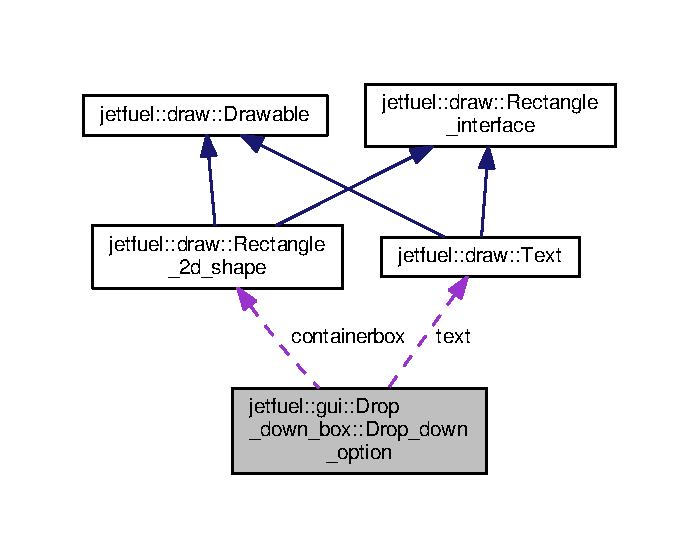
\includegraphics[width=336pt]{structjetfuel_1_1gui_1_1Drop__down__box_1_1Drop__down__option__coll__graph}
\end{center}
\end{figure}
\subsection*{Public Attributes}
\begin{DoxyCompactItemize}
\item 
\mbox{\Hypertarget{structjetfuel_1_1gui_1_1Drop__down__box_1_1Drop__down__option_a51183cc19b7ddff4e3fcefe46444b306}\label{structjetfuel_1_1gui_1_1Drop__down__box_1_1Drop__down__option_a51183cc19b7ddff4e3fcefe46444b306}} 
\hyperlink{classjetfuel_1_1draw_1_1Rectangle__2d__shape}{jetfuel\+::draw\+::\+Rectangle\+\_\+2d\+\_\+shape} {\bfseries containerbox}
\item 
\mbox{\Hypertarget{structjetfuel_1_1gui_1_1Drop__down__box_1_1Drop__down__option_aa007a6149c65af3128c930254365c7b5}\label{structjetfuel_1_1gui_1_1Drop__down__box_1_1Drop__down__option_aa007a6149c65af3128c930254365c7b5}} 
\hyperlink{classjetfuel_1_1draw_1_1Text}{jetfuel\+::draw\+::\+Text} {\bfseries text}
\end{DoxyCompactItemize}


The documentation for this struct was generated from the following file\+:\begin{DoxyCompactItemize}
\item 
include/jetfuelgui/dropdownbox.\+h\end{DoxyCompactItemize}

\hypertarget{classjetfuel_1_1draw_1_1Font}{}\section{jetfuel\+:\+:draw\+:\+:Font Class Reference}
\label{classjetfuel_1_1draw_1_1Font}\index{jetfuel\+::draw\+::\+Font@{jetfuel\+::draw\+::\+Font}}


{\ttfamily \#include $<$font.\+h$>$}

\subsection*{Public Member Functions}
\begin{DoxyCompactItemize}
\item 
\hyperlink{classjetfuel_1_1draw_1_1Font_a1054eb031ce0e8485f828f5ae7463770}{Font} ()
\begin{DoxyCompactList}\small\item\em Default constructor. \end{DoxyCompactList}\item 
\hyperlink{classjetfuel_1_1draw_1_1Font_a96db43b28c32511ff481502ec8d11fd7}{Font} (const std\+::string filename)
\begin{DoxyCompactList}\small\item\em Constructs a \hyperlink{classjetfuel_1_1draw_1_1Font}{Font} object with a filename. \end{DoxyCompactList}\item 
\hyperlink{classjetfuel_1_1draw_1_1Font_a5907cc1ecc14725d642ef5c3c753ced9}{Font} (const std\+::string filename, const long faceindex)
\begin{DoxyCompactList}\small\item\em Constructs a \hyperlink{classjetfuel_1_1draw_1_1Font}{Font} object with a filename and a face index. \end{DoxyCompactList}\item 
bool \hyperlink{classjetfuel_1_1draw_1_1Font_a23a8e0aed90fac334f939d1b10864976}{Is\+\_\+font\+\_\+loaded} () const
\begin{DoxyCompactList}\small\item\em Checks if the font is loaded. \end{DoxyCompactList}\item 
T\+T\+F\+\_\+\+Font $\ast$ \hyperlink{classjetfuel_1_1draw_1_1Font_aa6583c70e9b801b16dc78ca3a156bc97}{Get\+\_\+ttf\+\_\+font} () const
\begin{DoxyCompactList}\small\item\em Gets a reference to the T\+T\+F\+\_\+\+Font used by the library. \end{DoxyCompactList}\item 
std\+::string \hyperlink{classjetfuel_1_1draw_1_1Font_a497ce6fb60f71fdc8667c5a5ede81cca}{Get\+\_\+file\+\_\+name} () const
\begin{DoxyCompactList}\small\item\em Returns this \hyperlink{classjetfuel_1_1draw_1_1Font}{Font}\textquotesingle{}s filename. \end{DoxyCompactList}\item 
long \hyperlink{classjetfuel_1_1draw_1_1Font_ad0f24c27c3dcca9839e4ffc1603a1c54}{Get\+\_\+face\+\_\+index} () const
\begin{DoxyCompactList}\small\item\em Returns this \hyperlink{classjetfuel_1_1draw_1_1Font}{Font}\textquotesingle{}s face index. \end{DoxyCompactList}\item 
void \hyperlink{classjetfuel_1_1draw_1_1Font_a5b6bec15a5220e34f5138fe9f1abf72e}{Load\+\_\+font} (const std\+::string filename)
\begin{DoxyCompactList}\small\item\em Loads the font with a filename. \end{DoxyCompactList}\item 
void \hyperlink{classjetfuel_1_1draw_1_1Font_aac89368ac80b1dd5b7831f40af14ef2f}{Load\+\_\+font} (const std\+::string filename, const long faceindex)
\begin{DoxyCompactList}\small\item\em Loads the font with a filename and a face index. \end{DoxyCompactList}\item 
void \hyperlink{classjetfuel_1_1draw_1_1Font_a2a99e3273204f9dca27017c568f1eefe}{Change\+\_\+size} (const unsigned int size)
\begin{DoxyCompactList}\small\item\em Changes the point size of the \hyperlink{classjetfuel_1_1draw_1_1Font}{Font}. \end{DoxyCompactList}\end{DoxyCompactItemize}
\subsection*{Protected Member Functions}
\begin{DoxyCompactItemize}
\item 
void \hyperlink{classjetfuel_1_1draw_1_1Font_ac30b41dcdbdb87d103f0b976ac785560}{Set\+\_\+is\+\_\+font\+\_\+loaded} (bool isfontloaded=false)
\begin{DoxyCompactList}\small\item\em Set whether the font is loaded. \end{DoxyCompactList}\item 
void \hyperlink{classjetfuel_1_1draw_1_1Font_a42161bfb7213d0a5cbfb9dc4ad66348d}{Set\+\_\+file\+\_\+name} (const std\+::string filename)
\begin{DoxyCompactList}\small\item\em Set the filename of the \hyperlink{classjetfuel_1_1draw_1_1Font}{Font} object. \end{DoxyCompactList}\item 
void \hyperlink{classjetfuel_1_1draw_1_1Font_a0a8f47fbecce1093557f4d2e4c6266bf}{Set\+\_\+face\+\_\+index} (long faceindex=-\/1)
\begin{DoxyCompactList}\small\item\em Set the face index of the \hyperlink{classjetfuel_1_1draw_1_1Font}{Font} object. \end{DoxyCompactList}\item 
void \hyperlink{classjetfuel_1_1draw_1_1Font_a6238d89e07f1b9866c61ebd1ed26ef6a}{Set\+\_\+ttf\+\_\+font} (T\+T\+F\+\_\+\+Font $\ast$ttffont)
\begin{DoxyCompactList}\small\item\em Set the T\+T\+F\+\_\+\+Font reference. \end{DoxyCompactList}\item 
\mbox{\Hypertarget{classjetfuel_1_1draw_1_1Font_af8d15fa128f23cec34841f06fb3ec911}\label{classjetfuel_1_1draw_1_1Font_af8d15fa128f23cec34841f06fb3ec911}} 
void {\bfseries Set\+\_\+ttf\+\_\+init} (bool ttfinit)
\end{DoxyCompactItemize}
\subsection*{Static Protected Member Functions}
\begin{DoxyCompactItemize}
\item 
\mbox{\Hypertarget{classjetfuel_1_1draw_1_1Font_a20a6307ecb4da7363a877ad8786b6ff9}\label{classjetfuel_1_1draw_1_1Font_a20a6307ecb4da7363a877ad8786b6ff9}} 
static bool {\bfseries Get\+\_\+ttf\+\_\+init} ()
\end{DoxyCompactItemize}


\subsection{Detailed Description}
A True\+Type font object to be used in conjunction with a \hyperlink{classjetfuel_1_1draw_1_1Text}{jetfuel\+::draw\+::\+Text} object to display some text.

Code Example\+: \hyperlink{classjetfuel_1_1draw_1_1Scene__manager}{jetfuel\+::draw\+::\+Scene\+\_\+manager} scenemanager; \hyperlink{classjetfuel_1_1draw_1_1Scene}{jetfuel\+::draw\+::\+Scene} scene1; \hyperlink{classjetfuel_1_1draw_1_1Font}{jetfuel\+::draw\+::\+Font} font(\char`\"{}default.\+ttf\char`\"{}); \hyperlink{classjetfuel_1_1draw_1_1Text}{jetfuel\+::draw\+::\+Text} hello(font);

if(!scenemanager.Create\+\_\+window(\char`\"{}example\char`\"{}, jetfuel\+::draw\+::\+Vector2d\+\_\+int(0,0), jetfuel\+::draw\+::\+Vector2d\+\_\+int(500,500)))\{ std\+::cerr $<$$<$ \char`\"{}\mbox{[}!\mbox{]}\+E\+R\+R\+O\+R with creating sdl renderer!\char`\"{} $<$$<$ \char`\"{}\+Error is\+:\char`\"{} $<$$<$ S\+D\+L\+\_\+\+Get\+Error() $<$$<$ \char`\"{}\textbackslash{}n\char`\"{}; \}

if(!scenemanager.Create\+\_\+renderer())\{ std\+::cerr $<$$<$ \char`\"{}\mbox{[}!\mbox{]}\+E\+R\+R\+O\+R with creating sdl renderer!\char`\"{} $<$$<$ \char`\"{}\+Error is\+:\char`\"{} $<$$<$ S\+D\+L\+\_\+\+Get\+Error() $<$$<$ \char`\"{}\textbackslash{}n\char`\"{}; \}

scenemanager.\+Switch\+\_\+current\+\_\+scene(\&scene1);

hello.\+Set\+\_\+string(\char`\"{}\+Why Hello There\char`\"{}); hello.\+Set\+\_\+position(jetfuel\+::draw\+::\+Vector2d\+\_\+int(100,100)); hello.\+Set\+\_\+text\+\_\+color(jetfuel\+::draw\+::\+Color\+::\+Cyan); hello.\+Set\+\_\+font\+\_\+size(50); hello.\+Set\+\_\+render\+\_\+mode(jetfuel\+::draw\+::\+Text\+::\+Render\+\_\+mode\+::\+Blended);

scene1.\+Attach\+\_\+drawable(\&hello,1);

scenemanager.\+Draw\+\_\+current\+\_\+scene(); 

\subsection{Constructor \& Destructor Documentation}
\mbox{\Hypertarget{classjetfuel_1_1draw_1_1Font_a1054eb031ce0e8485f828f5ae7463770}\label{classjetfuel_1_1draw_1_1Font_a1054eb031ce0e8485f828f5ae7463770}} 
\index{jetfuel\+::draw\+::\+Font@{jetfuel\+::draw\+::\+Font}!Font@{Font}}
\index{Font@{Font}!jetfuel\+::draw\+::\+Font@{jetfuel\+::draw\+::\+Font}}
\subsubsection{\texorpdfstring{Font()}{Font()}\hspace{0.1cm}{\footnotesize\ttfamily [1/3]}}
{\footnotesize\ttfamily jetfuel\+::draw\+::\+Font\+::\+Font (\begin{DoxyParamCaption}{ }\end{DoxyParamCaption})\hspace{0.3cm}{\ttfamily [inline]}}



Default constructor. 

Constructs an empty \hyperlink{classjetfuel_1_1draw_1_1Font}{Font} object with the filename and (optionally) the face index to be set later. \mbox{\Hypertarget{classjetfuel_1_1draw_1_1Font_a96db43b28c32511ff481502ec8d11fd7}\label{classjetfuel_1_1draw_1_1Font_a96db43b28c32511ff481502ec8d11fd7}} 
\index{jetfuel\+::draw\+::\+Font@{jetfuel\+::draw\+::\+Font}!Font@{Font}}
\index{Font@{Font}!jetfuel\+::draw\+::\+Font@{jetfuel\+::draw\+::\+Font}}
\subsubsection{\texorpdfstring{Font()}{Font()}\hspace{0.1cm}{\footnotesize\ttfamily [2/3]}}
{\footnotesize\ttfamily jetfuel\+::draw\+::\+Font\+::\+Font (\begin{DoxyParamCaption}\item[{const std\+::string}]{filename }\end{DoxyParamCaption})}



Constructs a \hyperlink{classjetfuel_1_1draw_1_1Font}{Font} object with a filename. 

Constructs a \hyperlink{classjetfuel_1_1draw_1_1Font}{Font} object with a filename of where the True\+Type font file is located.


\begin{DoxyParams}{Parameters}
{\em std\+::string} & filename \\
\hline
\end{DoxyParams}
\mbox{\Hypertarget{classjetfuel_1_1draw_1_1Font_a5907cc1ecc14725d642ef5c3c753ced9}\label{classjetfuel_1_1draw_1_1Font_a5907cc1ecc14725d642ef5c3c753ced9}} 
\index{jetfuel\+::draw\+::\+Font@{jetfuel\+::draw\+::\+Font}!Font@{Font}}
\index{Font@{Font}!jetfuel\+::draw\+::\+Font@{jetfuel\+::draw\+::\+Font}}
\subsubsection{\texorpdfstring{Font()}{Font()}\hspace{0.1cm}{\footnotesize\ttfamily [3/3]}}
{\footnotesize\ttfamily jetfuel\+::draw\+::\+Font\+::\+Font (\begin{DoxyParamCaption}\item[{const std\+::string}]{filename,  }\item[{const long}]{faceindex }\end{DoxyParamCaption})}



Constructs a \hyperlink{classjetfuel_1_1draw_1_1Font}{Font} object with a filename and a face index. 

Constructs a \hyperlink{classjetfuel_1_1draw_1_1Font}{Font} object with a filename of where the True\+Type font file is located, and a face index for which face to open.


\begin{DoxyParams}{Parameters}
{\em std\+::string} & filename \\
\hline
{\em long} & faceindex \\
\hline
\end{DoxyParams}


\subsection{Member Function Documentation}
\mbox{\Hypertarget{classjetfuel_1_1draw_1_1Font_a2a99e3273204f9dca27017c568f1eefe}\label{classjetfuel_1_1draw_1_1Font_a2a99e3273204f9dca27017c568f1eefe}} 
\index{jetfuel\+::draw\+::\+Font@{jetfuel\+::draw\+::\+Font}!Change\+\_\+size@{Change\+\_\+size}}
\index{Change\+\_\+size@{Change\+\_\+size}!jetfuel\+::draw\+::\+Font@{jetfuel\+::draw\+::\+Font}}
\subsubsection{\texorpdfstring{Change\+\_\+size()}{Change\_size()}}
{\footnotesize\ttfamily void jetfuel\+::draw\+::\+Font\+::\+Change\+\_\+size (\begin{DoxyParamCaption}\item[{const unsigned int}]{size }\end{DoxyParamCaption})}



Changes the point size of the \hyperlink{classjetfuel_1_1draw_1_1Font}{Font}. 

Changes the point size of the \hyperlink{classjetfuel_1_1draw_1_1Font}{Font}. You should not use this function with just a \hyperlink{classjetfuel_1_1draw_1_1Font}{Font}. Instead, use \hyperlink{classjetfuel_1_1draw_1_1Text}{jetfuel\+::draw\+::\+Text}\textquotesingle{}s Set\+\_\+font\+\_\+size function change the size which calls this function to function anyways.


\begin{DoxyParams}{Parameters}
{\em int} & size \\
\hline
\end{DoxyParams}
\mbox{\Hypertarget{classjetfuel_1_1draw_1_1Font_ad0f24c27c3dcca9839e4ffc1603a1c54}\label{classjetfuel_1_1draw_1_1Font_ad0f24c27c3dcca9839e4ffc1603a1c54}} 
\index{jetfuel\+::draw\+::\+Font@{jetfuel\+::draw\+::\+Font}!Get\+\_\+face\+\_\+index@{Get\+\_\+face\+\_\+index}}
\index{Get\+\_\+face\+\_\+index@{Get\+\_\+face\+\_\+index}!jetfuel\+::draw\+::\+Font@{jetfuel\+::draw\+::\+Font}}
\subsubsection{\texorpdfstring{Get\+\_\+face\+\_\+index()}{Get\_face\_index()}}
{\footnotesize\ttfamily long jetfuel\+::draw\+::\+Font\+::\+Get\+\_\+face\+\_\+index (\begin{DoxyParamCaption}{ }\end{DoxyParamCaption}) const\hspace{0.3cm}{\ttfamily [inline]}}



Returns this \hyperlink{classjetfuel_1_1draw_1_1Font}{Font}\textquotesingle{}s face index. 

Returns this \hyperlink{classjetfuel_1_1draw_1_1Font}{Font}\textquotesingle{}s face index that it was loaded with or constructed with. \mbox{\Hypertarget{classjetfuel_1_1draw_1_1Font_a497ce6fb60f71fdc8667c5a5ede81cca}\label{classjetfuel_1_1draw_1_1Font_a497ce6fb60f71fdc8667c5a5ede81cca}} 
\index{jetfuel\+::draw\+::\+Font@{jetfuel\+::draw\+::\+Font}!Get\+\_\+file\+\_\+name@{Get\+\_\+file\+\_\+name}}
\index{Get\+\_\+file\+\_\+name@{Get\+\_\+file\+\_\+name}!jetfuel\+::draw\+::\+Font@{jetfuel\+::draw\+::\+Font}}
\subsubsection{\texorpdfstring{Get\+\_\+file\+\_\+name()}{Get\_file\_name()}}
{\footnotesize\ttfamily std\+::string jetfuel\+::draw\+::\+Font\+::\+Get\+\_\+file\+\_\+name (\begin{DoxyParamCaption}{ }\end{DoxyParamCaption}) const\hspace{0.3cm}{\ttfamily [inline]}}



Returns this \hyperlink{classjetfuel_1_1draw_1_1Font}{Font}\textquotesingle{}s filename. 

Returns this \hyperlink{classjetfuel_1_1draw_1_1Font}{Font}\textquotesingle{}s filename that it was loaded with or constructed with. \mbox{\Hypertarget{classjetfuel_1_1draw_1_1Font_aa6583c70e9b801b16dc78ca3a156bc97}\label{classjetfuel_1_1draw_1_1Font_aa6583c70e9b801b16dc78ca3a156bc97}} 
\index{jetfuel\+::draw\+::\+Font@{jetfuel\+::draw\+::\+Font}!Get\+\_\+ttf\+\_\+font@{Get\+\_\+ttf\+\_\+font}}
\index{Get\+\_\+ttf\+\_\+font@{Get\+\_\+ttf\+\_\+font}!jetfuel\+::draw\+::\+Font@{jetfuel\+::draw\+::\+Font}}
\subsubsection{\texorpdfstring{Get\+\_\+ttf\+\_\+font()}{Get\_ttf\_font()}}
{\footnotesize\ttfamily T\+T\+F\+\_\+\+Font$\ast$ jetfuel\+::draw\+::\+Font\+::\+Get\+\_\+ttf\+\_\+font (\begin{DoxyParamCaption}{ }\end{DoxyParamCaption}) const\hspace{0.3cm}{\ttfamily [inline]}}



Gets a reference to the T\+T\+F\+\_\+\+Font used by the library. 

Get a reference to the T\+T\+F\+\_\+\+Font used by the engine. If you fully utilize this engine and do not modify it\textquotesingle{}s internals, you should not have to call this function. \mbox{\Hypertarget{classjetfuel_1_1draw_1_1Font_a23a8e0aed90fac334f939d1b10864976}\label{classjetfuel_1_1draw_1_1Font_a23a8e0aed90fac334f939d1b10864976}} 
\index{jetfuel\+::draw\+::\+Font@{jetfuel\+::draw\+::\+Font}!Is\+\_\+font\+\_\+loaded@{Is\+\_\+font\+\_\+loaded}}
\index{Is\+\_\+font\+\_\+loaded@{Is\+\_\+font\+\_\+loaded}!jetfuel\+::draw\+::\+Font@{jetfuel\+::draw\+::\+Font}}
\subsubsection{\texorpdfstring{Is\+\_\+font\+\_\+loaded()}{Is\_font\_loaded()}}
{\footnotesize\ttfamily bool jetfuel\+::draw\+::\+Font\+::\+Is\+\_\+font\+\_\+loaded (\begin{DoxyParamCaption}{ }\end{DoxyParamCaption}) const\hspace{0.3cm}{\ttfamily [inline]}}



Checks if the font is loaded. 

Checks if the font is loaded. In other words, Check if at least a filename, and, optionally, a face index have been set. \mbox{\Hypertarget{classjetfuel_1_1draw_1_1Font_a5b6bec15a5220e34f5138fe9f1abf72e}\label{classjetfuel_1_1draw_1_1Font_a5b6bec15a5220e34f5138fe9f1abf72e}} 
\index{jetfuel\+::draw\+::\+Font@{jetfuel\+::draw\+::\+Font}!Load\+\_\+font@{Load\+\_\+font}}
\index{Load\+\_\+font@{Load\+\_\+font}!jetfuel\+::draw\+::\+Font@{jetfuel\+::draw\+::\+Font}}
\subsubsection{\texorpdfstring{Load\+\_\+font()}{Load\_font()}\hspace{0.1cm}{\footnotesize\ttfamily [1/2]}}
{\footnotesize\ttfamily void jetfuel\+::draw\+::\+Font\+::\+Load\+\_\+font (\begin{DoxyParamCaption}\item[{const std\+::string}]{filename }\end{DoxyParamCaption})}



Loads the font with a filename. 

Loads the font with a filename locating the True\+Type font file.


\begin{DoxyParams}{Parameters}
{\em std\+::string} & filename \\
\hline
\end{DoxyParams}
\mbox{\Hypertarget{classjetfuel_1_1draw_1_1Font_aac89368ac80b1dd5b7831f40af14ef2f}\label{classjetfuel_1_1draw_1_1Font_aac89368ac80b1dd5b7831f40af14ef2f}} 
\index{jetfuel\+::draw\+::\+Font@{jetfuel\+::draw\+::\+Font}!Load\+\_\+font@{Load\+\_\+font}}
\index{Load\+\_\+font@{Load\+\_\+font}!jetfuel\+::draw\+::\+Font@{jetfuel\+::draw\+::\+Font}}
\subsubsection{\texorpdfstring{Load\+\_\+font()}{Load\_font()}\hspace{0.1cm}{\footnotesize\ttfamily [2/2]}}
{\footnotesize\ttfamily void jetfuel\+::draw\+::\+Font\+::\+Load\+\_\+font (\begin{DoxyParamCaption}\item[{const std\+::string}]{filename,  }\item[{const long}]{faceindex }\end{DoxyParamCaption})}



Loads the font with a filename and a face index. 

Loads the font with a filename locating the True\+Type font file and a face index to indicate which face to use.


\begin{DoxyParams}{Parameters}
{\em std\+::string} & filename \\
\hline
{\em long} & faceindex \\
\hline
\end{DoxyParams}
\mbox{\Hypertarget{classjetfuel_1_1draw_1_1Font_a0a8f47fbecce1093557f4d2e4c6266bf}\label{classjetfuel_1_1draw_1_1Font_a0a8f47fbecce1093557f4d2e4c6266bf}} 
\index{jetfuel\+::draw\+::\+Font@{jetfuel\+::draw\+::\+Font}!Set\+\_\+face\+\_\+index@{Set\+\_\+face\+\_\+index}}
\index{Set\+\_\+face\+\_\+index@{Set\+\_\+face\+\_\+index}!jetfuel\+::draw\+::\+Font@{jetfuel\+::draw\+::\+Font}}
\subsubsection{\texorpdfstring{Set\+\_\+face\+\_\+index()}{Set\_face\_index()}}
{\footnotesize\ttfamily void jetfuel\+::draw\+::\+Font\+::\+Set\+\_\+face\+\_\+index (\begin{DoxyParamCaption}\item[{long}]{faceindex = {\ttfamily -\/1} }\end{DoxyParamCaption})\hspace{0.3cm}{\ttfamily [inline]}, {\ttfamily [protected]}}



Set the face index of the \hyperlink{classjetfuel_1_1draw_1_1Font}{Font} object. 

Set the face index of the \hyperlink{classjetfuel_1_1draw_1_1Font}{Font} object during construction or loading of the \hyperlink{classjetfuel_1_1draw_1_1Font}{Font} object. \mbox{\Hypertarget{classjetfuel_1_1draw_1_1Font_a42161bfb7213d0a5cbfb9dc4ad66348d}\label{classjetfuel_1_1draw_1_1Font_a42161bfb7213d0a5cbfb9dc4ad66348d}} 
\index{jetfuel\+::draw\+::\+Font@{jetfuel\+::draw\+::\+Font}!Set\+\_\+file\+\_\+name@{Set\+\_\+file\+\_\+name}}
\index{Set\+\_\+file\+\_\+name@{Set\+\_\+file\+\_\+name}!jetfuel\+::draw\+::\+Font@{jetfuel\+::draw\+::\+Font}}
\subsubsection{\texorpdfstring{Set\+\_\+file\+\_\+name()}{Set\_file\_name()}}
{\footnotesize\ttfamily void jetfuel\+::draw\+::\+Font\+::\+Set\+\_\+file\+\_\+name (\begin{DoxyParamCaption}\item[{const std\+::string}]{filename }\end{DoxyParamCaption})\hspace{0.3cm}{\ttfamily [inline]}, {\ttfamily [protected]}}



Set the filename of the \hyperlink{classjetfuel_1_1draw_1_1Font}{Font} object. 

Set the filename of the \hyperlink{classjetfuel_1_1draw_1_1Font}{Font} object during construction or loading of the \hyperlink{classjetfuel_1_1draw_1_1Font}{Font} object.


\begin{DoxyParams}{Parameters}
{\em std\+::string} & filename \\
\hline
\end{DoxyParams}
\mbox{\Hypertarget{classjetfuel_1_1draw_1_1Font_ac30b41dcdbdb87d103f0b976ac785560}\label{classjetfuel_1_1draw_1_1Font_ac30b41dcdbdb87d103f0b976ac785560}} 
\index{jetfuel\+::draw\+::\+Font@{jetfuel\+::draw\+::\+Font}!Set\+\_\+is\+\_\+font\+\_\+loaded@{Set\+\_\+is\+\_\+font\+\_\+loaded}}
\index{Set\+\_\+is\+\_\+font\+\_\+loaded@{Set\+\_\+is\+\_\+font\+\_\+loaded}!jetfuel\+::draw\+::\+Font@{jetfuel\+::draw\+::\+Font}}
\subsubsection{\texorpdfstring{Set\+\_\+is\+\_\+font\+\_\+loaded()}{Set\_is\_font\_loaded()}}
{\footnotesize\ttfamily void jetfuel\+::draw\+::\+Font\+::\+Set\+\_\+is\+\_\+font\+\_\+loaded (\begin{DoxyParamCaption}\item[{bool}]{isfontloaded = {\ttfamily false} }\end{DoxyParamCaption})\hspace{0.3cm}{\ttfamily [inline]}, {\ttfamily [protected]}}



Set whether the font is loaded. 

Set whether the font is loaded when constructing or loading a font.


\begin{DoxyParams}{Parameters}
{\em bool} & isfontloaded \\
\hline
\end{DoxyParams}
\mbox{\Hypertarget{classjetfuel_1_1draw_1_1Font_a6238d89e07f1b9866c61ebd1ed26ef6a}\label{classjetfuel_1_1draw_1_1Font_a6238d89e07f1b9866c61ebd1ed26ef6a}} 
\index{jetfuel\+::draw\+::\+Font@{jetfuel\+::draw\+::\+Font}!Set\+\_\+ttf\+\_\+font@{Set\+\_\+ttf\+\_\+font}}
\index{Set\+\_\+ttf\+\_\+font@{Set\+\_\+ttf\+\_\+font}!jetfuel\+::draw\+::\+Font@{jetfuel\+::draw\+::\+Font}}
\subsubsection{\texorpdfstring{Set\+\_\+ttf\+\_\+font()}{Set\_ttf\_font()}}
{\footnotesize\ttfamily void jetfuel\+::draw\+::\+Font\+::\+Set\+\_\+ttf\+\_\+font (\begin{DoxyParamCaption}\item[{T\+T\+F\+\_\+\+Font $\ast$}]{ttffont }\end{DoxyParamCaption})\hspace{0.3cm}{\ttfamily [inline]}, {\ttfamily [protected]}}



Set the T\+T\+F\+\_\+\+Font reference. 

Set the T\+T\+F\+\_\+\+Font reference used when creating text. 

The documentation for this class was generated from the following file\+:\begin{DoxyCompactItemize}
\item 
include/jetfueldraw/font.\+h\end{DoxyCompactItemize}

\hypertarget{classjetfuel_1_1draw_1_1exceptions_1_1Font__not__init__exception}{}\section{jetfuel\+:\+:draw\+:\+:exceptions\+:\+:Font\+\_\+not\+\_\+init\+\_\+exception Class Reference}
\label{classjetfuel_1_1draw_1_1exceptions_1_1Font__not__init__exception}\index{jetfuel\+::draw\+::exceptions\+::\+Font\+\_\+not\+\_\+init\+\_\+exception@{jetfuel\+::draw\+::exceptions\+::\+Font\+\_\+not\+\_\+init\+\_\+exception}}


{\ttfamily \#include $<$text.\+h$>$}



Inheritance diagram for jetfuel\+:\+:draw\+:\+:exceptions\+:\+:Font\+\_\+not\+\_\+init\+\_\+exception\+:\nopagebreak
\begin{figure}[H]
\begin{center}
\leavevmode
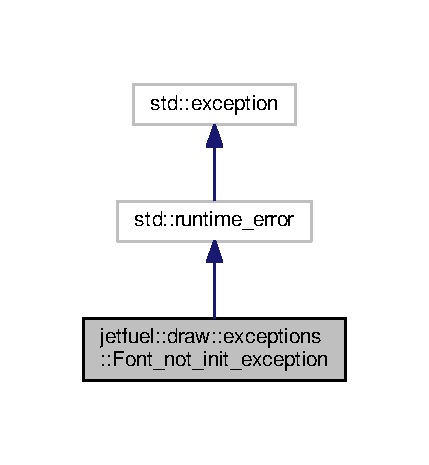
\includegraphics[width=206pt]{classjetfuel_1_1draw_1_1exceptions_1_1Font__not__init__exception__inherit__graph}
\end{center}
\end{figure}


Collaboration diagram for jetfuel\+:\+:draw\+:\+:exceptions\+:\+:Font\+\_\+not\+\_\+init\+\_\+exception\+:\nopagebreak
\begin{figure}[H]
\begin{center}
\leavevmode
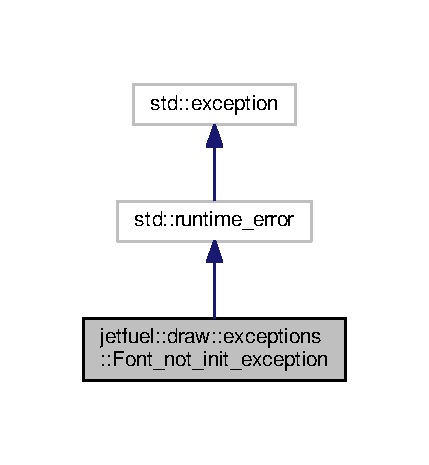
\includegraphics[width=206pt]{classjetfuel_1_1draw_1_1exceptions_1_1Font__not__init__exception__coll__graph}
\end{center}
\end{figure}
\subsection*{Public Member Functions}
\begin{DoxyCompactItemize}
\item 
\hyperlink{classjetfuel_1_1draw_1_1exceptions_1_1Font__not__init__exception_af3e44125242cd74a0c2694abc15bec86}{Font\+\_\+not\+\_\+init\+\_\+exception} ()
\begin{DoxyCompactList}\small\item\em Constructs a \hyperlink{classjetfuel_1_1draw_1_1exceptions_1_1Font__not__init__exception}{Font\+\_\+not\+\_\+init\+\_\+exception}. \end{DoxyCompactList}\end{DoxyCompactItemize}


\subsection{Detailed Description}
This exception should be thrown when a font passed into a function as an argument is not loaded and ready for the class to use it. This exception is not meant to be used outside of the \hyperlink{classjetfuel_1_1draw_1_1Text}{Text} class.

Code Example\+: 
\begin{DoxyCode}
\textcolor{keywordtype}{void} Do\_something\_with\_font(Font font)\{
    \textcolor{keywordflow}{if}(font.Is\_font\_loaded())\{
        \textcolor{comment}{// do something with the font...}
    \}\textcolor{keywordflow}{else}\{
        \textcolor{keywordflow}{throw} jetfuel::draw::exceptions::
              Font\_not\_init\_exception();
    \}
\}
\end{DoxyCode}
 

\subsection{Constructor \& Destructor Documentation}
\mbox{\Hypertarget{classjetfuel_1_1draw_1_1exceptions_1_1Font__not__init__exception_af3e44125242cd74a0c2694abc15bec86}\label{classjetfuel_1_1draw_1_1exceptions_1_1Font__not__init__exception_af3e44125242cd74a0c2694abc15bec86}} 
\index{jetfuel\+::draw\+::exceptions\+::\+Font\+\_\+not\+\_\+init\+\_\+exception@{jetfuel\+::draw\+::exceptions\+::\+Font\+\_\+not\+\_\+init\+\_\+exception}!Font\+\_\+not\+\_\+init\+\_\+exception@{Font\+\_\+not\+\_\+init\+\_\+exception}}
\index{Font\+\_\+not\+\_\+init\+\_\+exception@{Font\+\_\+not\+\_\+init\+\_\+exception}!jetfuel\+::draw\+::exceptions\+::\+Font\+\_\+not\+\_\+init\+\_\+exception@{jetfuel\+::draw\+::exceptions\+::\+Font\+\_\+not\+\_\+init\+\_\+exception}}
\subsubsection{\texorpdfstring{Font\+\_\+not\+\_\+init\+\_\+exception()}{Font\_not\_init\_exception()}}
{\footnotesize\ttfamily jetfuel\+::draw\+::exceptions\+::\+Font\+\_\+not\+\_\+init\+\_\+exception\+::\+Font\+\_\+not\+\_\+init\+\_\+exception (\begin{DoxyParamCaption}{ }\end{DoxyParamCaption})\hspace{0.3cm}{\ttfamily [inline]}}



Constructs a \hyperlink{classjetfuel_1_1draw_1_1exceptions_1_1Font__not__init__exception}{Font\+\_\+not\+\_\+init\+\_\+exception}. 

Constructs a \hyperlink{classjetfuel_1_1draw_1_1exceptions_1_1Font__not__init__exception}{Font\+\_\+not\+\_\+init\+\_\+exception}. 

The documentation for this class was generated from the following file\+:\begin{DoxyCompactItemize}
\item 
include/jetfueldraw/text.\+h\end{DoxyCompactItemize}

\hypertarget{classjetfuel_1_1gui_1_1IClickable}{}\section{jetfuel\+:\+:gui\+:\+:I\+Clickable Class Reference}
\label{classjetfuel_1_1gui_1_1IClickable}\index{jetfuel\+::gui\+::\+I\+Clickable@{jetfuel\+::gui\+::\+I\+Clickable}}


{\ttfamily \#include $<$iclickable.\+h$>$}



Inheritance diagram for jetfuel\+:\+:gui\+:\+:I\+Clickable\+:
\nopagebreak
\begin{figure}[H]
\begin{center}
\leavevmode
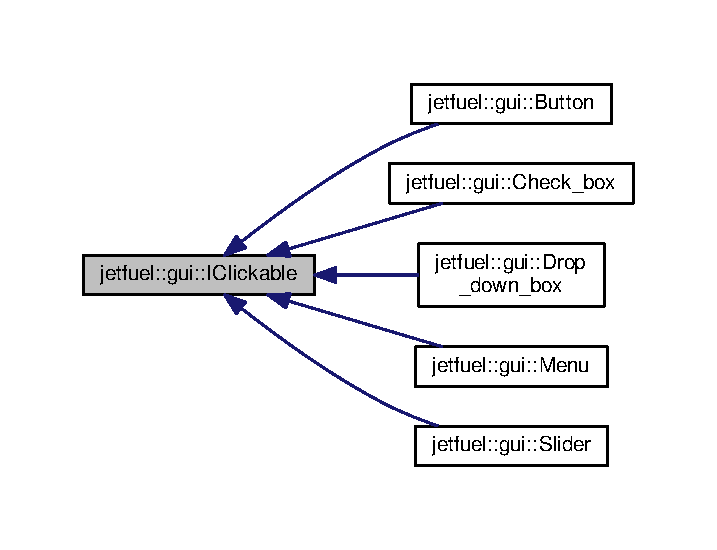
\includegraphics[width=344pt]{classjetfuel_1_1gui_1_1IClickable__inherit__graph}
\end{center}
\end{figure}
\subsection*{Public Member Functions}
\begin{DoxyCompactItemize}
\item 
virtual void \hyperlink{classjetfuel_1_1gui_1_1IClickable_aea45de37bd3beb7eb7e2e3056e4e37b3}{Check\+\_\+for\+\_\+clicks} (\hyperlink{structjetfuel_1_1control_1_1Action}{jetfuel\+::control\+::\+Action} U\+I\+Sinterpreterdata)=0
\begin{DoxyCompactList}\small\item\em Checks for clicks on this object. \end{DoxyCompactList}\end{DoxyCompactItemize}


\subsection{Detailed Description}
A simple interface that clickable object should inherit.

\begin{DoxySeeAlso}{See also}
\hyperlink{classjetfuel_1_1gui_1_1Button}{jetfuel\+::gui\+::\+Button} 

\hyperlink{classjetfuel_1_1gui_1_1Check__box}{jetfuel\+::gui\+::\+Check\+\_\+box} 

\hyperlink{classjetfuel_1_1gui_1_1Drop__down__box}{jetfuel\+::gui\+::\+Drop\+\_\+down\+\_\+box} 
\end{DoxySeeAlso}


\subsection{Member Function Documentation}
\mbox{\Hypertarget{classjetfuel_1_1gui_1_1IClickable_aea45de37bd3beb7eb7e2e3056e4e37b3}\label{classjetfuel_1_1gui_1_1IClickable_aea45de37bd3beb7eb7e2e3056e4e37b3}} 
\index{jetfuel\+::gui\+::\+I\+Clickable@{jetfuel\+::gui\+::\+I\+Clickable}!Check\+\_\+for\+\_\+clicks@{Check\+\_\+for\+\_\+clicks}}
\index{Check\+\_\+for\+\_\+clicks@{Check\+\_\+for\+\_\+clicks}!jetfuel\+::gui\+::\+I\+Clickable@{jetfuel\+::gui\+::\+I\+Clickable}}
\subsubsection{\texorpdfstring{Check\+\_\+for\+\_\+clicks()}{Check\_for\_clicks()}}
{\footnotesize\ttfamily virtual void jetfuel\+::gui\+::\+I\+Clickable\+::\+Check\+\_\+for\+\_\+clicks (\begin{DoxyParamCaption}\item[{\hyperlink{structjetfuel_1_1control_1_1Action}{jetfuel\+::control\+::\+Action}}]{U\+I\+Sinterpreterdata }\end{DoxyParamCaption})\hspace{0.3cm}{\ttfamily [pure virtual]}}



Checks for clicks on this object. 

Checks for clicks on this object, based upon the Universal Input System Action.

This is a pure virtual function that must be implemented by any children of this interface.


\begin{DoxyParams}{Parameters}
{\em \hyperlink{structjetfuel_1_1control_1_1Action}{jetfuel\+::control\+::\+Action}} & U\+I\+Sinterpreterdata \\
\hline
\end{DoxyParams}


Implemented in \hyperlink{classjetfuel_1_1gui_1_1Menu_a17298e1cec290db84ab4e3b1b13bd614}{jetfuel\+::gui\+::\+Menu}, \hyperlink{classjetfuel_1_1gui_1_1Check__box_a0e50420591dbd64f07f02f9ee7cec637}{jetfuel\+::gui\+::\+Check\+\_\+box}, \hyperlink{classjetfuel_1_1gui_1_1Slider_a8a1e83cfea8d65db34da7447dce9fb6f}{jetfuel\+::gui\+::\+Slider}, \hyperlink{classjetfuel_1_1gui_1_1Drop__down__box_ae3607405b7e3fe981da75f0529e0a7a1}{jetfuel\+::gui\+::\+Drop\+\_\+down\+\_\+box}, \hyperlink{classjetfuel_1_1gui_1_1Text__box_a088d62b01be4747ea2e7a6218516e036}{jetfuel\+::gui\+::\+Text\+\_\+box}, and \hyperlink{classjetfuel_1_1gui_1_1Button_ab80239583f2e515370a90771976c5265}{jetfuel\+::gui\+::\+Button}.



The documentation for this class was generated from the following file\+:\begin{DoxyCompactItemize}
\item 
include/jetfuelgui/iclickable.\+h\end{DoxyCompactItemize}

\hypertarget{classjetfuel_1_1draw_1_1Image}{}\section{jetfuel\+:\+:draw\+:\+:Image Class Reference}
\label{classjetfuel_1_1draw_1_1Image}\index{jetfuel\+::draw\+::\+Image@{jetfuel\+::draw\+::\+Image}}


{\ttfamily \#include $<$image.\+h$>$}

\subsection*{Public Member Functions}
\begin{DoxyCompactItemize}
\item 
\hyperlink{classjetfuel_1_1draw_1_1Image_a63078fc295eb37ef549e17187d839574}{Image} ()
\begin{DoxyCompactList}\small\item\em Default constructor. \end{DoxyCompactList}\item 
\hyperlink{classjetfuel_1_1draw_1_1Image_a36c7a9de74ed515a90b5688d7efb040c}{Image} (const std\+::string imagepath, \hyperlink{classjetfuel_1_1draw_1_1Scene__manager}{Scene\+\_\+manager} $\ast$scenemanager)
\begin{DoxyCompactList}\small\item\em Constructs an image with an image path and a scene manager. \end{DoxyCompactList}\item 
\hyperlink{classjetfuel_1_1draw_1_1Image_a80771f30728e311a58d7e0fa5844a6d5}{Image} (const std\+::string imagepath, const \hyperlink{classjetfuel_1_1draw_1_1Vector2d}{Vector2d\+\_\+int} imagesize)
\begin{DoxyCompactList}\small\item\em Constructs an image with an image path and an image size, without the need of a \hyperlink{classjetfuel_1_1draw_1_1Scene__manager}{Scene\+\_\+manager}. \end{DoxyCompactList}\item 
void \hyperlink{classjetfuel_1_1draw_1_1Image_a2259992a6ae87fdebfe088f07a7bcc4e}{Set\+\_\+image} (const std\+::string imagepath, \hyperlink{classjetfuel_1_1draw_1_1Scene__manager}{Scene\+\_\+manager} $\ast$scenemanager)
\begin{DoxyCompactList}\small\item\em Sets an image path and a scene manager. \end{DoxyCompactList}\item 
void \hyperlink{classjetfuel_1_1draw_1_1Image_a4b445f5105eaed28d9a18d6bf3ed44bb}{Set\+\_\+image} (const std\+::string imagepath, const \hyperlink{classjetfuel_1_1draw_1_1Vector2d}{Vector2d\+\_\+int} imagesize)
\begin{DoxyCompactList}\small\item\em Sets an image with an image path and an image size, without the need of a \hyperlink{classjetfuel_1_1draw_1_1Scene__manager}{Scene\+\_\+manager}. \end{DoxyCompactList}\item 
std\+::string \hyperlink{classjetfuel_1_1draw_1_1Image_afe13a343f0ca098c2f258511fa6a2f2b}{Get\+\_\+image\+\_\+location} () const
\begin{DoxyCompactList}\small\item\em Returns the image\textquotesingle{}s location. \end{DoxyCompactList}\item 
\hyperlink{classjetfuel_1_1draw_1_1Vector2d}{jetfuel\+::draw\+::\+Vector2d\+\_\+int} \hyperlink{classjetfuel_1_1draw_1_1Image_a69eb09128ebcbf427eac516d0c042ce5}{Get\+\_\+size\+\_\+of\+\_\+image} () const
\begin{DoxyCompactList}\small\item\em Returns the image\textquotesingle{}s size (in pixels) \end{DoxyCompactList}\item 
std\+::string \hyperlink{classjetfuel_1_1draw_1_1Image_a4014f980cf67b0716b57b48f7a98020e}{Get\+\_\+error} ()
\begin{DoxyCompactList}\small\item\em Gets S\+D\+L\+\_\+image error, if any. \end{DoxyCompactList}\end{DoxyCompactItemize}
\subsection*{Protected Member Functions}
\begin{DoxyCompactItemize}
\item 
void \hyperlink{classjetfuel_1_1draw_1_1Image_a0426e7dcc92eb1220cc8d1a508bdcca8}{Set\+\_\+image\+\_\+location} (const std\+::string imagelocation)
\begin{DoxyCompactList}\small\item\em Sets the image location. \end{DoxyCompactList}\item 
void \hyperlink{classjetfuel_1_1draw_1_1Image_a9252d59e532f26b94572f155c4d4b118}{Set\+\_\+size\+\_\+of\+\_\+image} (const \hyperlink{classjetfuel_1_1draw_1_1Vector2d}{Vector2d\+\_\+int} imagesize)
\begin{DoxyCompactList}\small\item\em Sets the size of the image. \end{DoxyCompactList}\end{DoxyCompactItemize}


\subsection{Detailed Description}
A image to be used with a \hyperlink{classjetfuel_1_1draw_1_1Sprite}{Sprite} to display images. This image is a simple wrapper to be used with a \hyperlink{classjetfuel_1_1draw_1_1Sprite}{Sprite} that stores the filepath of an image and the size of an image.

Code Example\+: \hyperlink{classjetfuel_1_1draw_1_1Scene__manager}{jetfuel\+::draw\+::\+Scene\+\_\+manager} scenemanager; \hyperlink{classjetfuel_1_1draw_1_1Scene}{jetfuel\+::draw\+::\+Scene} scene1(1); \hyperlink{classjetfuel_1_1draw_1_1Image}{jetfuel\+::draw\+::\+Image} image = \hyperlink{classjetfuel_1_1draw_1_1Image}{jetfuel\+::draw\+::\+Image}(\char`\"{}test.\+png\char`\"{}, \&scenemanager); \hyperlink{classjetfuel_1_1draw_1_1Sprite}{jetfuel\+::draw\+::\+Sprite} background;

if(!scenemanager.Create\+\_\+window(\char`\"{}example\char`\"{}, jetfuel\+::draw\+::\+Vector2d\+\_\+int(0,0), jetfuel\+::draw\+::\+Vector2d\+\_\+int(500,500)))\{ std\+::cerr $<$$<$ \char`\"{}\mbox{[}!\mbox{]}\+E\+R\+R\+O\+R with creating sdl renderer!\char`\"{} $<$$<$ \char`\"{}\+Error is\+:\char`\"{} $<$$<$ S\+D\+L\+\_\+\+Get\+Error() $<$$<$ \char`\"{}\textbackslash{}n\char`\"{}; \}

if(!scenemanager.Create\+\_\+renderer())\{ std\+::cerr $<$$<$ \char`\"{}\mbox{[}!\mbox{]}\+E\+R\+R\+O\+R with creating sdl renderer!\char`\"{} $<$$<$ \char`\"{}\+Error is\+:\char`\"{} $<$$<$ S\+D\+L\+\_\+\+Get\+Error() $<$$<$ \char`\"{}\textbackslash{}n\char`\"{}; \}

scenemanager.\+Switch\+\_\+current\+\_\+scene(\&scene1); scene1.\+Attach\+\_\+drawable(\&background,1);

if(!background.Load\+\_\+from\+\_\+image(backgroundimage))\{ std\+::cerr $<$$<$ \char`\"{}\mbox{[}!\mbox{]}\+E\+R\+R\+O\+R with loading from image! Error is\+:\char`\"{} $<$$<$ backgroundimage.\+Get\+\_\+error $<$$<$ \char`\"{}\textbackslash{}n\char`\"{};

return 1; \}

background.\+Set\+\_\+position(jetfuel\+::draw\+::\+Vector2d\+\_\+int(0,0));

scenemanager.\+Draw\+\_\+current\+\_\+scene(); 

\subsection{Constructor \& Destructor Documentation}
\mbox{\Hypertarget{classjetfuel_1_1draw_1_1Image_a63078fc295eb37ef549e17187d839574}\label{classjetfuel_1_1draw_1_1Image_a63078fc295eb37ef549e17187d839574}} 
\index{jetfuel\+::draw\+::\+Image@{jetfuel\+::draw\+::\+Image}!Image@{Image}}
\index{Image@{Image}!jetfuel\+::draw\+::\+Image@{jetfuel\+::draw\+::\+Image}}
\subsubsection{\texorpdfstring{Image()}{Image()}\hspace{0.1cm}{\footnotesize\ttfamily [1/3]}}
{\footnotesize\ttfamily jetfuel\+::draw\+::\+Image\+::\+Image (\begin{DoxyParamCaption}{ }\end{DoxyParamCaption})\hspace{0.3cm}{\ttfamily [inline]}}



Default constructor. 

Initializes an \hyperlink{classjetfuel_1_1draw_1_1Image}{Image} with an image path and an image size to be set later. \mbox{\Hypertarget{classjetfuel_1_1draw_1_1Image_a36c7a9de74ed515a90b5688d7efb040c}\label{classjetfuel_1_1draw_1_1Image_a36c7a9de74ed515a90b5688d7efb040c}} 
\index{jetfuel\+::draw\+::\+Image@{jetfuel\+::draw\+::\+Image}!Image@{Image}}
\index{Image@{Image}!jetfuel\+::draw\+::\+Image@{jetfuel\+::draw\+::\+Image}}
\subsubsection{\texorpdfstring{Image()}{Image()}\hspace{0.1cm}{\footnotesize\ttfamily [2/3]}}
{\footnotesize\ttfamily jetfuel\+::draw\+::\+Image\+::\+Image (\begin{DoxyParamCaption}\item[{const std\+::string}]{imagepath,  }\item[{\hyperlink{classjetfuel_1_1draw_1_1Scene__manager}{Scene\+\_\+manager} $\ast$}]{scenemanager }\end{DoxyParamCaption})}



Constructs an image with an image path and a scene manager. 

Initializes an \hyperlink{classjetfuel_1_1draw_1_1Image}{Image} with an image path and an scene manager, so that the image is ready to be used by a \hyperlink{classjetfuel_1_1draw_1_1Sprite}{Sprite}.


\begin{DoxyParams}{Parameters}
{\em std\+::string} & imagepath \\
\hline
{\em \hyperlink{classjetfuel_1_1draw_1_1Scene__manager}{jetfuel\+::draw\+::\+Scene\+\_\+manager}} & $\ast$scenemanager \\
\hline
\end{DoxyParams}
\mbox{\Hypertarget{classjetfuel_1_1draw_1_1Image_a80771f30728e311a58d7e0fa5844a6d5}\label{classjetfuel_1_1draw_1_1Image_a80771f30728e311a58d7e0fa5844a6d5}} 
\index{jetfuel\+::draw\+::\+Image@{jetfuel\+::draw\+::\+Image}!Image@{Image}}
\index{Image@{Image}!jetfuel\+::draw\+::\+Image@{jetfuel\+::draw\+::\+Image}}
\subsubsection{\texorpdfstring{Image()}{Image()}\hspace{0.1cm}{\footnotesize\ttfamily [3/3]}}
{\footnotesize\ttfamily jetfuel\+::draw\+::\+Image\+::\+Image (\begin{DoxyParamCaption}\item[{const std\+::string}]{imagepath,  }\item[{const \hyperlink{classjetfuel_1_1draw_1_1Vector2d}{Vector2d\+\_\+int}}]{imagesize }\end{DoxyParamCaption})}



Constructs an image with an image path and an image size, without the need of a \hyperlink{classjetfuel_1_1draw_1_1Scene__manager}{Scene\+\_\+manager}. 

Constructs an image with an image path and an image size, without the need of a \hyperlink{classjetfuel_1_1draw_1_1Scene__manager}{Scene\+\_\+manager} so that an image is ready to be used by a \hyperlink{classjetfuel_1_1draw_1_1Sprite}{Sprite}.


\begin{DoxyParams}{Parameters}
{\em std\+::string} & imagepath \\
\hline
{\em jetfuel\+::draw\+::\+Vector2d\+\_\+int} & imagesize \\
\hline
\end{DoxyParams}


\subsection{Member Function Documentation}
\mbox{\Hypertarget{classjetfuel_1_1draw_1_1Image_a4014f980cf67b0716b57b48f7a98020e}\label{classjetfuel_1_1draw_1_1Image_a4014f980cf67b0716b57b48f7a98020e}} 
\index{jetfuel\+::draw\+::\+Image@{jetfuel\+::draw\+::\+Image}!Get\+\_\+error@{Get\+\_\+error}}
\index{Get\+\_\+error@{Get\+\_\+error}!jetfuel\+::draw\+::\+Image@{jetfuel\+::draw\+::\+Image}}
\subsubsection{\texorpdfstring{Get\+\_\+error()}{Get\_error()}}
{\footnotesize\ttfamily std\+::string jetfuel\+::draw\+::\+Image\+::\+Get\+\_\+error (\begin{DoxyParamCaption}{ }\end{DoxyParamCaption})\hspace{0.3cm}{\ttfamily [inline]}}



Gets S\+D\+L\+\_\+image error, if any. 

Gets S\+D\+L\+\_\+image error, if any. This function is useful to call when something goes wrong with this \hyperlink{classjetfuel_1_1draw_1_1Image}{Image} class. \mbox{\Hypertarget{classjetfuel_1_1draw_1_1Image_afe13a343f0ca098c2f258511fa6a2f2b}\label{classjetfuel_1_1draw_1_1Image_afe13a343f0ca098c2f258511fa6a2f2b}} 
\index{jetfuel\+::draw\+::\+Image@{jetfuel\+::draw\+::\+Image}!Get\+\_\+image\+\_\+location@{Get\+\_\+image\+\_\+location}}
\index{Get\+\_\+image\+\_\+location@{Get\+\_\+image\+\_\+location}!jetfuel\+::draw\+::\+Image@{jetfuel\+::draw\+::\+Image}}
\subsubsection{\texorpdfstring{Get\+\_\+image\+\_\+location()}{Get\_image\_location()}}
{\footnotesize\ttfamily std\+::string jetfuel\+::draw\+::\+Image\+::\+Get\+\_\+image\+\_\+location (\begin{DoxyParamCaption}{ }\end{DoxyParamCaption}) const\hspace{0.3cm}{\ttfamily [inline]}}



Returns the image\textquotesingle{}s location. 

Returns the image\textquotesingle{}s location (or path) to load in a \hyperlink{classjetfuel_1_1draw_1_1Sprite}{Sprite}. \mbox{\Hypertarget{classjetfuel_1_1draw_1_1Image_a69eb09128ebcbf427eac516d0c042ce5}\label{classjetfuel_1_1draw_1_1Image_a69eb09128ebcbf427eac516d0c042ce5}} 
\index{jetfuel\+::draw\+::\+Image@{jetfuel\+::draw\+::\+Image}!Get\+\_\+size\+\_\+of\+\_\+image@{Get\+\_\+size\+\_\+of\+\_\+image}}
\index{Get\+\_\+size\+\_\+of\+\_\+image@{Get\+\_\+size\+\_\+of\+\_\+image}!jetfuel\+::draw\+::\+Image@{jetfuel\+::draw\+::\+Image}}
\subsubsection{\texorpdfstring{Get\+\_\+size\+\_\+of\+\_\+image()}{Get\_size\_of\_image()}}
{\footnotesize\ttfamily \hyperlink{classjetfuel_1_1draw_1_1Vector2d}{jetfuel\+::draw\+::\+Vector2d\+\_\+int} jetfuel\+::draw\+::\+Image\+::\+Get\+\_\+size\+\_\+of\+\_\+image (\begin{DoxyParamCaption}{ }\end{DoxyParamCaption}) const\hspace{0.3cm}{\ttfamily [inline]}}



Returns the image\textquotesingle{}s size (in pixels) 

Returns the image\textquotesingle{}s size as given as calculated with a \hyperlink{classjetfuel_1_1draw_1_1Scene__manager}{Scene\+\_\+manager} or given to this class via an argument. \mbox{\Hypertarget{classjetfuel_1_1draw_1_1Image_a2259992a6ae87fdebfe088f07a7bcc4e}\label{classjetfuel_1_1draw_1_1Image_a2259992a6ae87fdebfe088f07a7bcc4e}} 
\index{jetfuel\+::draw\+::\+Image@{jetfuel\+::draw\+::\+Image}!Set\+\_\+image@{Set\+\_\+image}}
\index{Set\+\_\+image@{Set\+\_\+image}!jetfuel\+::draw\+::\+Image@{jetfuel\+::draw\+::\+Image}}
\subsubsection{\texorpdfstring{Set\+\_\+image()}{Set\_image()}\hspace{0.1cm}{\footnotesize\ttfamily [1/2]}}
{\footnotesize\ttfamily void jetfuel\+::draw\+::\+Image\+::\+Set\+\_\+image (\begin{DoxyParamCaption}\item[{const std\+::string}]{imagepath,  }\item[{\hyperlink{classjetfuel_1_1draw_1_1Scene__manager}{Scene\+\_\+manager} $\ast$}]{scenemanager }\end{DoxyParamCaption})}



Sets an image path and a scene manager. 

Sets an image path and an scene manager after an \hyperlink{classjetfuel_1_1draw_1_1Image}{Image} has been constructed. This function is especially useful when using the default constructor, as you need to set the image path and a scene manager or image size later.


\begin{DoxyParams}{Parameters}
{\em std\+::string} & imagepath \\
\hline
{\em \hyperlink{classjetfuel_1_1draw_1_1Scene__manager}{jetfuel\+::draw\+::\+Scene\+\_\+manager}} & $\ast$scenemanager \\
\hline
\end{DoxyParams}
\mbox{\Hypertarget{classjetfuel_1_1draw_1_1Image_a4b445f5105eaed28d9a18d6bf3ed44bb}\label{classjetfuel_1_1draw_1_1Image_a4b445f5105eaed28d9a18d6bf3ed44bb}} 
\index{jetfuel\+::draw\+::\+Image@{jetfuel\+::draw\+::\+Image}!Set\+\_\+image@{Set\+\_\+image}}
\index{Set\+\_\+image@{Set\+\_\+image}!jetfuel\+::draw\+::\+Image@{jetfuel\+::draw\+::\+Image}}
\subsubsection{\texorpdfstring{Set\+\_\+image()}{Set\_image()}\hspace{0.1cm}{\footnotesize\ttfamily [2/2]}}
{\footnotesize\ttfamily void jetfuel\+::draw\+::\+Image\+::\+Set\+\_\+image (\begin{DoxyParamCaption}\item[{const std\+::string}]{imagepath,  }\item[{const \hyperlink{classjetfuel_1_1draw_1_1Vector2d}{Vector2d\+\_\+int}}]{imagesize }\end{DoxyParamCaption})}



Sets an image with an image path and an image size, without the need of a \hyperlink{classjetfuel_1_1draw_1_1Scene__manager}{Scene\+\_\+manager}. 

Sets an image with an image path and an image size, without the need of a \hyperlink{classjetfuel_1_1draw_1_1Scene__manager}{Scene\+\_\+manager} so that an image is ready to be used by a \hyperlink{classjetfuel_1_1draw_1_1Sprite}{Sprite}.

This function is especially useful when using the default constructor, as you need to set the image path and a scene manager or image size later.


\begin{DoxyParams}{Parameters}
{\em std\+::string} & imagepath \\
\hline
{\em jetfuel\+::draw\+::\+Vector2d\+\_\+int} & imagesize \\
\hline
\end{DoxyParams}
\mbox{\Hypertarget{classjetfuel_1_1draw_1_1Image_a0426e7dcc92eb1220cc8d1a508bdcca8}\label{classjetfuel_1_1draw_1_1Image_a0426e7dcc92eb1220cc8d1a508bdcca8}} 
\index{jetfuel\+::draw\+::\+Image@{jetfuel\+::draw\+::\+Image}!Set\+\_\+image\+\_\+location@{Set\+\_\+image\+\_\+location}}
\index{Set\+\_\+image\+\_\+location@{Set\+\_\+image\+\_\+location}!jetfuel\+::draw\+::\+Image@{jetfuel\+::draw\+::\+Image}}
\subsubsection{\texorpdfstring{Set\+\_\+image\+\_\+location()}{Set\_image\_location()}}
{\footnotesize\ttfamily void jetfuel\+::draw\+::\+Image\+::\+Set\+\_\+image\+\_\+location (\begin{DoxyParamCaption}\item[{const std\+::string}]{imagelocation }\end{DoxyParamCaption})\hspace{0.3cm}{\ttfamily [inline]}, {\ttfamily [protected]}}



Sets the image location. 

Sets the image file location to be used when loading this image.


\begin{DoxyParams}{Parameters}
{\em std\+::string} & imagelocation \\
\hline
\end{DoxyParams}
\mbox{\Hypertarget{classjetfuel_1_1draw_1_1Image_a9252d59e532f26b94572f155c4d4b118}\label{classjetfuel_1_1draw_1_1Image_a9252d59e532f26b94572f155c4d4b118}} 
\index{jetfuel\+::draw\+::\+Image@{jetfuel\+::draw\+::\+Image}!Set\+\_\+size\+\_\+of\+\_\+image@{Set\+\_\+size\+\_\+of\+\_\+image}}
\index{Set\+\_\+size\+\_\+of\+\_\+image@{Set\+\_\+size\+\_\+of\+\_\+image}!jetfuel\+::draw\+::\+Image@{jetfuel\+::draw\+::\+Image}}
\subsubsection{\texorpdfstring{Set\+\_\+size\+\_\+of\+\_\+image()}{Set\_size\_of\_image()}}
{\footnotesize\ttfamily void jetfuel\+::draw\+::\+Image\+::\+Set\+\_\+size\+\_\+of\+\_\+image (\begin{DoxyParamCaption}\item[{const \hyperlink{classjetfuel_1_1draw_1_1Vector2d}{Vector2d\+\_\+int}}]{imagesize }\end{DoxyParamCaption})\hspace{0.3cm}{\ttfamily [inline]}, {\ttfamily [protected]}}



Sets the size of the image. 

Sets the size of the image to be used when drawing and positioning this image.


\begin{DoxyParams}{Parameters}
{\em Vector2d\+\_\+int} & imagesize \\
\hline
\end{DoxyParams}


The documentation for this class was generated from the following file\+:\begin{DoxyCompactItemize}
\item 
include/jetfueldraw/image.\+h\end{DoxyCompactItemize}

\hypertarget{structjetfuel_1_1locale_1_1Locale__string}{}\section{jetfuel\+:\+:locale\+:\+:Locale\+\_\+string Struct Reference}
\label{structjetfuel_1_1locale_1_1Locale__string}\index{jetfuel\+::locale\+::\+Locale\+\_\+string@{jetfuel\+::locale\+::\+Locale\+\_\+string}}


{\ttfamily \#include $<$stringlocalefile.\+h$>$}



Collaboration diagram for jetfuel\+:\+:locale\+:\+:Locale\+\_\+string\+:
\nopagebreak
\begin{figure}[H]
\begin{center}
\leavevmode
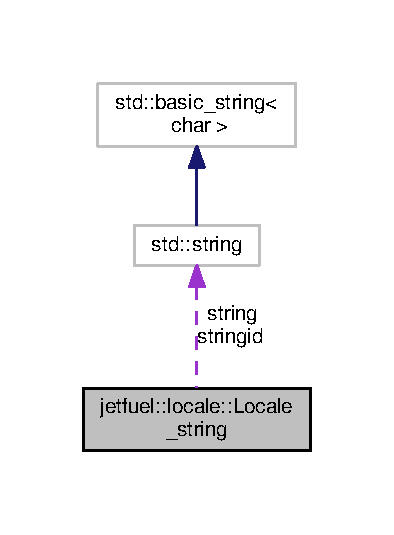
\includegraphics[width=189pt]{structjetfuel_1_1locale_1_1Locale__string__coll__graph}
\end{center}
\end{figure}
\subsection*{Public Attributes}
\begin{DoxyCompactItemize}
\item 
\mbox{\Hypertarget{structjetfuel_1_1locale_1_1Locale__string_a7e6246a99dcae8a12968a1fac0dd81cc}\label{structjetfuel_1_1locale_1_1Locale__string_a7e6246a99dcae8a12968a1fac0dd81cc}} 
std\+::string {\bfseries stringid}
\item 
\mbox{\Hypertarget{structjetfuel_1_1locale_1_1Locale__string_a9cd781f5676a7a4b66b06559f177eaab}\label{structjetfuel_1_1locale_1_1Locale__string_a9cd781f5676a7a4b66b06559f177eaab}} 
std\+::string {\bfseries string}
\end{DoxyCompactItemize}


\subsection{Detailed Description}
A simple struct representing a localized string, with an id and the actual string.

\begin{DoxySeeAlso}{See also}
\hyperlink{classjetfuel_1_1locale_1_1String__locale__file}{jetfuel\+::locale\+::\+String\+\_\+locale\+\_\+file} 

\hyperlink{classjetfuel_1_1locale_1_1String__locale__manager}{jetfuel\+::locale\+::\+String\+\_\+locale\+\_\+manager} 
\end{DoxySeeAlso}


The documentation for this struct was generated from the following file\+:\begin{DoxyCompactItemize}
\item 
include/jetfuellocale/stringlocalefile.\+h\end{DoxyCompactItemize}

\hypertarget{classjetfuel_1_1gui_1_1Menu}{}\section{jetfuel\+:\+:gui\+:\+:Menu Class Reference}
\label{classjetfuel_1_1gui_1_1Menu}\index{jetfuel\+::gui\+::\+Menu@{jetfuel\+::gui\+::\+Menu}}


{\ttfamily \#include $<$menu.\+h$>$}



Inheritance diagram for jetfuel\+:\+:gui\+:\+:Menu\+:\nopagebreak
\begin{figure}[H]
\begin{center}
\leavevmode
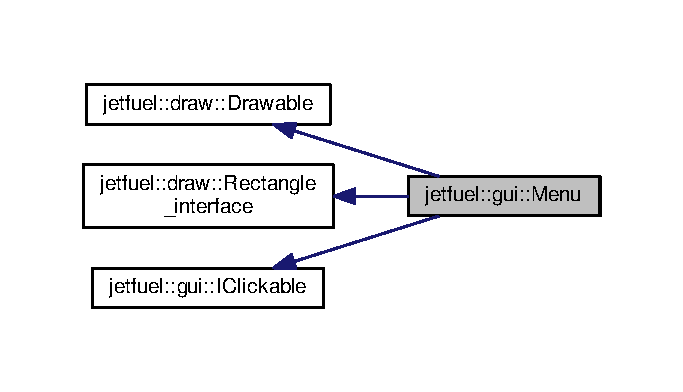
\includegraphics[width=328pt]{classjetfuel_1_1gui_1_1Menu__inherit__graph}
\end{center}
\end{figure}


Collaboration diagram for jetfuel\+:\+:gui\+:\+:Menu\+:\nopagebreak
\begin{figure}[H]
\begin{center}
\leavevmode
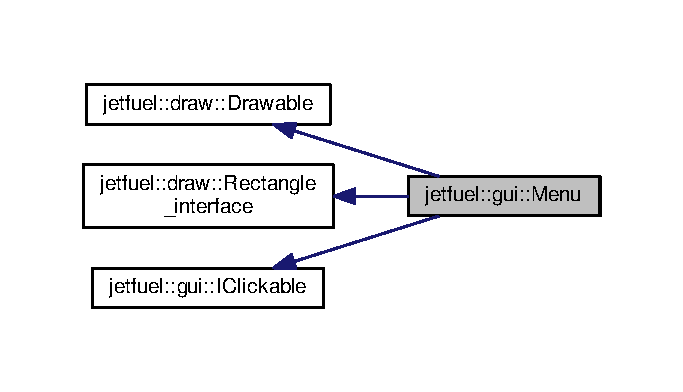
\includegraphics[width=328pt]{classjetfuel_1_1gui_1_1Menu__coll__graph}
\end{center}
\end{figure}
\subsection*{Classes}
\begin{DoxyCompactItemize}
\item 
struct \hyperlink{structjetfuel_1_1gui_1_1Menu_1_1Button__characteristics}{Button\+\_\+characteristics}
\end{DoxyCompactItemize}
\subsection*{Public Member Functions}
\begin{DoxyCompactItemize}
\item 
\hyperlink{classjetfuel_1_1gui_1_1Menu_a8cdd5967a5c57fd28924ac5f9c979398}{Menu} ()
\begin{DoxyCompactList}\small\item\em Default constructor. \end{DoxyCompactList}\item 
\hyperlink{classjetfuel_1_1gui_1_1Menu_ae09bc951a919594033f94c5d827889d1}{Menu} (const unsigned int maxheight, const unsigned int columngap, const unsigned int buttongap)
\begin{DoxyCompactList}\small\item\em Constructs a \hyperlink{classjetfuel_1_1gui_1_1Menu}{Menu} with a max height, column gap, and button gap numbers. \end{DoxyCompactList}\item 
unsigned int \hyperlink{classjetfuel_1_1gui_1_1Menu_a9610775609d7243a9b4ac0c6e57a7aa3}{Get\+\_\+max\+\_\+height} () const
\begin{DoxyCompactList}\small\item\em Gets this \hyperlink{classjetfuel_1_1gui_1_1Menu}{Menu}\textquotesingle{}s max height for it\textquotesingle{}s buttons. \end{DoxyCompactList}\item 
void \hyperlink{classjetfuel_1_1gui_1_1Menu_ad713403a103dc547c7ae968bb6d5e2cd}{Set\+\_\+max\+\_\+height} (const unsigned int maxheight)
\begin{DoxyCompactList}\small\item\em Sets this \hyperlink{classjetfuel_1_1gui_1_1Menu}{Menu}\textquotesingle{}s max height for it\textquotesingle{}s buttons. \end{DoxyCompactList}\item 
unsigned int \hyperlink{classjetfuel_1_1gui_1_1Menu_a52a091ea0c745c1e09752a1766a8f262}{Get\+\_\+column\+\_\+gap} () const
\begin{DoxyCompactList}\small\item\em Gets this \hyperlink{classjetfuel_1_1gui_1_1Menu}{Menu}\textquotesingle{}s column gap for it\textquotesingle{}s buttons. \end{DoxyCompactList}\item 
void \hyperlink{classjetfuel_1_1gui_1_1Menu_a584ce362f2efe836a9cfff9729eac913}{Set\+\_\+column\+\_\+gap} (const unsigned int columngap)
\begin{DoxyCompactList}\small\item\em Sets this \hyperlink{classjetfuel_1_1gui_1_1Menu}{Menu}\textquotesingle{}s column gap for it\textquotesingle{}s buttons. \end{DoxyCompactList}\item 
unsigned int \hyperlink{classjetfuel_1_1gui_1_1Menu_a6ce40fbb47e1d6f6602092a4f4520bee}{Get\+\_\+button\+\_\+gap} () const
\begin{DoxyCompactList}\small\item\em Gets this \hyperlink{classjetfuel_1_1gui_1_1Menu}{Menu}\textquotesingle{}s button gap for it\textquotesingle{}s buttons. \end{DoxyCompactList}\item 
void \hyperlink{classjetfuel_1_1gui_1_1Menu_a8b715d2e92f18b77eb78e7a8e4fc8208}{Set\+\_\+button\+\_\+gap} (const unsigned int buttongap)
\begin{DoxyCompactList}\small\item\em Sets this \hyperlink{classjetfuel_1_1gui_1_1Menu}{Menu}\textquotesingle{}s button gap for it\textquotesingle{}s buttons. \end{DoxyCompactList}\item 
\hyperlink{classjetfuel_1_1draw_1_1Image}{jetfuel\+::draw\+::\+Image} \hyperlink{classjetfuel_1_1gui_1_1Menu_a6657e617308d99482c12f544fb88173c}{Get\+\_\+container\+\_\+box\+\_\+image} () const
\begin{DoxyCompactList}\small\item\em Gets the Buttons\textquotesingle{} container box image of this \hyperlink{classjetfuel_1_1gui_1_1Menu}{Menu} (could be empty if not set). \end{DoxyCompactList}\item 
void \hyperlink{classjetfuel_1_1gui_1_1Menu_a3ddedd81c865929157751c7857716318}{Set\+\_\+container\+\_\+box\+\_\+image} (const \hyperlink{classjetfuel_1_1draw_1_1Image}{jetfuel\+::draw\+::\+Image} containerboximage, const \hyperlink{classjetfuel_1_1draw_1_1Vector2d}{jetfuel\+::draw\+::\+Vector2d\+\_\+uint} containerboxborder)
\begin{DoxyCompactList}\small\item\em Sets the Buttons\textquotesingle{} container box image of this \hyperlink{classjetfuel_1_1gui_1_1Menu}{Menu}. \end{DoxyCompactList}\item 
\hyperlink{classjetfuel_1_1draw_1_1Vector2d}{jetfuel\+::draw\+::\+Vector2d\+\_\+uint} \hyperlink{classjetfuel_1_1gui_1_1Menu_aa8dbb384542c547ff90cdfeea1ff07eb}{Get\+\_\+container\+\_\+box\+\_\+border} () const
\begin{DoxyCompactList}\small\item\em Gets the Buttons\textquotesingle{} contain box borders (could be empty if not set). \end{DoxyCompactList}\item 
bool \hyperlink{classjetfuel_1_1gui_1_1Menu_a6f0162b01dbf0bd6bf65cfb3712499fc}{Add\+\_\+button} (\hyperlink{structjetfuel_1_1gui_1_1Menu_1_1Button__characteristics}{Button\+\_\+characteristics} buttonchars, const std\+::string U\+I\+Sactiontowatchfor, const std\+::string messagetosenduponclick, \hyperlink{classjetfuel_1_1core_1_1Message__bus}{jetfuel\+::core\+::\+Message\+\_\+bus} $\ast$bus, bool dynamicallyloadimage=false)
\begin{DoxyCompactList}\small\item\em Adds a button to this \hyperlink{classjetfuel_1_1gui_1_1Menu}{Menu}. \end{DoxyCompactList}\item 
void \hyperlink{classjetfuel_1_1gui_1_1Menu_acf4a69ccd0ee1490d02fa005c8eba1b4}{Assign\+\_\+renderer} (S\+D\+L\+\_\+\+Renderer $\ast$renderer) override
\begin{DoxyCompactList}\small\item\em Assigns a S\+DL renderer to this \hyperlink{classjetfuel_1_1gui_1_1Menu}{Menu}\textquotesingle{}s objects. \end{DoxyCompactList}\item 
S\+D\+L\+\_\+\+Renderer $\ast$ \hyperlink{classjetfuel_1_1gui_1_1Menu_a411940386454af4e44dc8c0c84c00215}{Get\+\_\+renderer} () override
\begin{DoxyCompactList}\small\item\em Gets the S\+DL renderer previously assigned. \end{DoxyCompactList}\item 
\hyperlink{classjetfuel_1_1draw_1_1Vector2d}{jetfuel\+::draw\+::\+Vector2d\+\_\+int} \hyperlink{classjetfuel_1_1gui_1_1Menu_ac1aebb753feba17be808f2068ff17e74}{Get\+\_\+position} () override
\begin{DoxyCompactList}\small\item\em Gets this \hyperlink{classjetfuel_1_1gui_1_1Menu}{Menu}\textquotesingle{}s position. \end{DoxyCompactList}\item 
void \hyperlink{classjetfuel_1_1gui_1_1Menu_ab575d5e4ad9d86d6781012e7d1bebc9a}{Set\+\_\+position} (\hyperlink{classjetfuel_1_1draw_1_1Vector2d}{jetfuel\+::draw\+::\+Vector2d\+\_\+int} position) override
\begin{DoxyCompactList}\small\item\em Sets this \hyperlink{classjetfuel_1_1gui_1_1Menu}{Menu}\textquotesingle{}s position. \end{DoxyCompactList}\item 
\hyperlink{classjetfuel_1_1draw_1_1Rect2d}{jetfuel\+::draw\+::\+Rect2d\+\_\+int} \hyperlink{classjetfuel_1_1gui_1_1Menu_a1d5c050dcad48008898eafe2d610eff6}{Get\+\_\+rect\+\_\+to\+\_\+draw} () override
\begin{DoxyCompactList}\small\item\em Gets this \hyperlink{classjetfuel_1_1gui_1_1Menu}{Menu}\textquotesingle{}s rect to be drawn when the Draw function is called. \end{DoxyCompactList}\item 
void \hyperlink{classjetfuel_1_1gui_1_1Menu_a17298e1cec290db84ab4e3b1b13bd614}{Check\+\_\+for\+\_\+clicks} (\hyperlink{structjetfuel_1_1control_1_1Action}{jetfuel\+::control\+::\+Action} U\+I\+Sinterpreterdata) override
\begin{DoxyCompactList}\small\item\em Checks for clicks on this \hyperlink{classjetfuel_1_1gui_1_1Menu}{Menu}\textquotesingle{}s buttons. \end{DoxyCompactList}\item 
bool \hyperlink{classjetfuel_1_1gui_1_1Menu_a0355f5ee3060b1ae9d85a5c8cba3795b}{Draw} () override
\begin{DoxyCompactList}\small\item\em Draws this \hyperlink{classjetfuel_1_1gui_1_1Menu}{Menu} on the screen. \end{DoxyCompactList}\end{DoxyCompactItemize}
\subsection*{Protected Member Functions}
\begin{DoxyCompactItemize}
\item 
unsigned int \hyperlink{classjetfuel_1_1gui_1_1Menu_abb5c42472d2bcc1338d694ce6cb35a13}{Get\+\_\+size\+\_\+of\+\_\+buttons\+\_\+vector} () const
\begin{DoxyCompactList}\small\item\em Gets the size of private m\+\_\+buttons vector. \end{DoxyCompactList}\item 
\hyperlink{classjetfuel_1_1gui_1_1Button}{Button} $\ast$ \hyperlink{classjetfuel_1_1gui_1_1Menu_a82ebabbd98cac6a1adf4ade59af57536}{Get\+\_\+button\+\_\+in\+\_\+buttons\+\_\+vector} (const size\+\_\+t whichbutton)
\begin{DoxyCompactList}\small\item\em Gets a certain button in the private m\+\_\+buttons vector. \end{DoxyCompactList}\item 
bool \hyperlink{classjetfuel_1_1gui_1_1Menu_ac30478425fc7feea544bad7f4dbad560}{Use\+\_\+container\+\_\+boxes} () const
\begin{DoxyCompactList}\small\item\em Returns whether this \hyperlink{classjetfuel_1_1gui_1_1Menu}{Menu} uses container boxes. \end{DoxyCompactList}\item 
size\+\_\+t \hyperlink{classjetfuel_1_1gui_1_1Menu_a93d17a47970afa6375eb4d9913338481}{Get\+\_\+size\+\_\+of\+\_\+container\+\_\+boxes\+\_\+vector} () const
\begin{DoxyCompactList}\small\item\em Gets the size of the private m\+\_\+containerboxes vector. \end{DoxyCompactList}\item 
\hyperlink{classjetfuel_1_1draw_1_1Sprite}{jetfuel\+::draw\+::\+Sprite} $\ast$ \hyperlink{classjetfuel_1_1gui_1_1Menu_a9f4a74b0103a6912e9236d1a66068aca}{Get\+\_\+box\+\_\+in\+\_\+container\+\_\+boxes\+\_\+vector} (const size\+\_\+t whichbox)
\begin{DoxyCompactList}\small\item\em Gets a certain box in the private m\+\_\+containerboxes vector. \end{DoxyCompactList}\item 
bool \hyperlink{classjetfuel_1_1gui_1_1Menu_a311940611ef799e82a1d412618c6206a}{Does\+\_\+container\+\_\+box\+\_\+exist\+\_\+inside\+\_\+vector} (const \hyperlink{classjetfuel_1_1draw_1_1Vector2d}{jetfuel\+::draw\+::\+Vector2d\+\_\+int} withwhatposition)
\begin{DoxyCompactList}\small\item\em Checks whether a container box exists inside the private m\+\_\+containerboxes vector. \end{DoxyCompactList}\item 
\hyperlink{classjetfuel_1_1draw_1_1Image}{jetfuel\+::draw\+::\+Image} \hyperlink{classjetfuel_1_1gui_1_1Menu_a0e59c1130398764ba7880ae38ba755e3}{Get\+\_\+button\+\_\+image\+\_\+in\+\_\+vector} (const size\+\_\+t whichimage) const
\begin{DoxyCompactList}\small\item\em Gets a \hyperlink{classjetfuel_1_1gui_1_1Button}{Button}\textquotesingle{}s image from the private m\+\_\+buttonimages vector. \end{DoxyCompactList}\item 
void \hyperlink{classjetfuel_1_1gui_1_1Menu_a265f704501aa00be0bc2059729896d55}{Push\+\_\+back\+\_\+into\+\_\+button\+\_\+image\+\_\+vector} (\hyperlink{classjetfuel_1_1draw_1_1Image}{jetfuel\+::draw\+::\+Image} image)
\begin{DoxyCompactList}\small\item\em Pushes back an image into the private m\+\_\+buttonimages vector. \end{DoxyCompactList}\item 
void \hyperlink{classjetfuel_1_1gui_1_1Menu_aa685f56941a8d70eafe30fb325abf38d}{Push\+\_\+back\+\_\+container\+\_\+box} (\hyperlink{classjetfuel_1_1draw_1_1Sprite}{jetfuel\+::draw\+::\+Sprite} box)
\begin{DoxyCompactList}\small\item\em Pushes back a container box Sprite into the private m\+\_\+containerboxes vector. \end{DoxyCompactList}\item 
void \hyperlink{classjetfuel_1_1gui_1_1Menu_a1efd742a6622d24a3ed6ae6a05fcba63}{Create\+\_\+container\+\_\+box} (\hyperlink{classjetfuel_1_1draw_1_1Vector2d}{jetfuel\+::draw\+::\+Vector2d\+\_\+int} position)
\begin{DoxyCompactList}\small\item\em Creates a container box with a position. \end{DoxyCompactList}\item 
\hyperlink{classjetfuel_1_1draw_1_1Vector2d}{jetfuel\+::draw\+::\+Vector2d\+\_\+int} \hyperlink{classjetfuel_1_1gui_1_1Menu_a9432e513bdc7deefab9da0f596144dc5}{Determine\+\_\+button\+\_\+position} (unsigned int whichbutton)
\begin{DoxyCompactList}\small\item\em Determines where a button should go based upon it\textquotesingle{}s button number. \end{DoxyCompactList}\end{DoxyCompactItemize}


\subsection{Detailed Description}
A simple collection of Buttons, with an option to have a container box image around it.

Code Example\+: 
\begin{DoxyCode}
\hyperlink{classjetfuel_1_1draw_1_1Scene__manager}{jetfuel::draw::Scene\_manager} scenemanager;
\hyperlink{classjetfuel_1_1draw_1_1Scene}{jetfuel::draw::Scene} scene1(1);
\hyperlink{classjetfuel_1_1core_1_1Message__bus}{jetfuel::core::Message\_bus} messagebus;
\hyperlink{classjetfuel_1_1gui_1_1Menu}{jetfuel::gui::Menu} menu;
\hyperlink{classjetfuel_1_1draw_1_1Image}{jetfuel::draw::Image} buttonimage;
\hyperlink{classjetfuel_1_1draw_1_1Image}{jetfuel::draw::Image} menuboximage(\textcolor{stringliteral}{"menubasebox.png"},
                                          &scenemanager);
\hyperlink{classjetfuel_1_1control_1_1UIS__manager}{jetfuel::control::UIS\_manager} UISmanager(&messagebus,
                                  scenemanager.\hyperlink{classjetfuel_1_1draw_1_1Scene__manager_a1758a86d40dcfaface8958fcd33676bf}{Get\_window\_id}());
\hyperlink{classjetfuel_1_1control_1_1UIS__interpreter}{jetfuel::control::UIS\_interpreter} UISinterpreter(&messagebus);
\hyperlink{structjetfuel_1_1draw_1_1Text_1_1Text__characteristics}{jetfuel::draw::Text::Text\_characteristics} textchars;
\hyperlink{structjetfuel_1_1gui_1_1Menu_1_1Button__characteristics}{jetfuel::gui::Menu::Button\_characteristics} buttonchars;
\hyperlink{classjetfuel_1_1draw_1_1Font}{jetfuel::draw::Font} font(\textcolor{stringliteral}{"default.ttf"});

\textcolor{keywordflow}{if}(!scenemanager.\hyperlink{classjetfuel_1_1draw_1_1Scene__manager_a5113e9062c272a22d383ba872417ba31}{Create\_window}(\textcolor{stringliteral}{"Hello Menus!"},
                               \hyperlink{classjetfuel_1_1draw_1_1Vector2d}{jetfuel::draw::Vector2d\_int}(0,0),
                          \hyperlink{classjetfuel_1_1draw_1_1Vector2d}{jetfuel::draw::Vector2d\_int}(640,480)))\{
    std::cout << \textcolor{stringliteral}{"[!]ERROR with creating sdl window! Error is:"}
    << SDL\_GetError() << \textcolor{stringliteral}{"\(\backslash\)n"};
\}

\textcolor{keywordflow}{if}(!scenemanager.\hyperlink{classjetfuel_1_1draw_1_1Scene__manager_afafecd926ce5e4b2543a6d583a7d24b6}{Create\_renderer}())\{
    std::cout << \textcolor{stringliteral}{"[!]ERROR with creating sdl renderer! Error is:"}
    << SDL\_GetError() << \textcolor{stringliteral}{"\(\backslash\)n"};
\}
scenemanager.\hyperlink{classjetfuel_1_1draw_1_1Scene__manager_a770c163b88ba8427539ee182315ea989}{Switch\_current\_scene}(&scene1);
scene1.\hyperlink{classjetfuel_1_1draw_1_1Scene_aea4b4c4ae25c30d661be4c52787e0ea3}{Attach\_drawable}(&menu,1);

\textcolor{keywordflow}{if}(!menu.Load\_base\_box\_image(menuboximage,
                             \hyperlink{classjetfuel_1_1draw_1_1Color_ab75797c1cb6e4dd952037916db39b5e8}{jetfuel::draw::Color::White},
                             \hyperlink{classjetfuel_1_1draw_1_1Vector2d}{jetfuel::draw::Vector2d\_uint}(
                                                    45,20)))\{
    std::cerr << \textcolor{stringliteral}{"[!]ERROR with loading from image! Error is:"} <<
    IMG\_GetError() << \textcolor{stringliteral}{"\(\backslash\)n"};
\}

menu.\hyperlink{classjetfuel_1_1gui_1_1Menu_ab575d5e4ad9d86d6781012e7d1bebc9a}{Set\_position}(\hyperlink{classjetfuel_1_1draw_1_1Vector2d}{jetfuel::draw::Vector2d\_int}(0,0));

textchars.textstring = \textcolor{stringliteral}{"resume"};
textchars.font = font;

resumechars.buttontextchars = textchars;

textchars.textstring = \textcolor{stringliteral}{"quit"};

quitchars.buttontextchars = textchars;

buttonimage.\hyperlink{classjetfuel_1_1draw_1_1Image_a2259992a6ae87fdebfe088f07a7bcc4e}{Set\_image}(\textcolor{stringliteral}{"button.png"},&scenemanager);
resumechars.image = buttonimage;
quitchars.image = buttonimage;

resumebutton.color = \hyperlink{classjetfuel_1_1draw_1_1Color}{jetfuel::draw::Color}(0, 255, 0, 100);
quitbutton.color = \hyperlink{classjetfuel_1_1draw_1_1Color}{jetfuel::draw::Color}(255, 0, 0, 100);

scenemanager.\hyperlink{classjetfuel_1_1draw_1_1Scene__manager_a8af9a3abfd5121b1b8556342de435773}{Draw\_current\_scene}();
\end{DoxyCode}
 

\subsection{Constructor \& Destructor Documentation}
\mbox{\Hypertarget{classjetfuel_1_1gui_1_1Menu_a8cdd5967a5c57fd28924ac5f9c979398}\label{classjetfuel_1_1gui_1_1Menu_a8cdd5967a5c57fd28924ac5f9c979398}} 
\index{jetfuel\+::gui\+::\+Menu@{jetfuel\+::gui\+::\+Menu}!Menu@{Menu}}
\index{Menu@{Menu}!jetfuel\+::gui\+::\+Menu@{jetfuel\+::gui\+::\+Menu}}
\subsubsection{\texorpdfstring{Menu()}{Menu()}\hspace{0.1cm}{\footnotesize\ttfamily [1/2]}}
{\footnotesize\ttfamily jetfuel\+::gui\+::\+Menu\+::\+Menu (\begin{DoxyParamCaption}{ }\end{DoxyParamCaption})\hspace{0.3cm}{\ttfamily [inline]}}



Default constructor. 

Default constructor. \mbox{\Hypertarget{classjetfuel_1_1gui_1_1Menu_ae09bc951a919594033f94c5d827889d1}\label{classjetfuel_1_1gui_1_1Menu_ae09bc951a919594033f94c5d827889d1}} 
\index{jetfuel\+::gui\+::\+Menu@{jetfuel\+::gui\+::\+Menu}!Menu@{Menu}}
\index{Menu@{Menu}!jetfuel\+::gui\+::\+Menu@{jetfuel\+::gui\+::\+Menu}}
\subsubsection{\texorpdfstring{Menu()}{Menu()}\hspace{0.1cm}{\footnotesize\ttfamily [2/2]}}
{\footnotesize\ttfamily jetfuel\+::gui\+::\+Menu\+::\+Menu (\begin{DoxyParamCaption}\item[{const unsigned int}]{maxheight,  }\item[{const unsigned int}]{columngap,  }\item[{const unsigned int}]{buttongap }\end{DoxyParamCaption})\hspace{0.3cm}{\ttfamily [inline]}}



Constructs a \hyperlink{classjetfuel_1_1gui_1_1Menu}{Menu} with a max height, column gap, and button gap numbers. 

Constructs a \hyperlink{classjetfuel_1_1gui_1_1Menu}{Menu} with a max height, column gap, and button gap numbers. 

\subsection{Member Function Documentation}
\mbox{\Hypertarget{classjetfuel_1_1gui_1_1Menu_a6f0162b01dbf0bd6bf65cfb3712499fc}\label{classjetfuel_1_1gui_1_1Menu_a6f0162b01dbf0bd6bf65cfb3712499fc}} 
\index{jetfuel\+::gui\+::\+Menu@{jetfuel\+::gui\+::\+Menu}!Add\+\_\+button@{Add\+\_\+button}}
\index{Add\+\_\+button@{Add\+\_\+button}!jetfuel\+::gui\+::\+Menu@{jetfuel\+::gui\+::\+Menu}}
\subsubsection{\texorpdfstring{Add\+\_\+button()}{Add\_button()}}
{\footnotesize\ttfamily bool jetfuel\+::gui\+::\+Menu\+::\+Add\+\_\+button (\begin{DoxyParamCaption}\item[{\hyperlink{structjetfuel_1_1gui_1_1Menu_1_1Button__characteristics}{Button\+\_\+characteristics}}]{buttonchars,  }\item[{const std\+::string}]{U\+I\+Sactiontowatchfor,  }\item[{const std\+::string}]{messagetosenduponclick,  }\item[{\hyperlink{classjetfuel_1_1core_1_1Message__bus}{jetfuel\+::core\+::\+Message\+\_\+bus} $\ast$}]{bus,  }\item[{bool}]{dynamicallyloadimage = {\ttfamily false} }\end{DoxyParamCaption})}



Adds a button to this \hyperlink{classjetfuel_1_1gui_1_1Menu}{Menu}. 

Adds a button, with button characteristics, an action to watch for, a meessage to send upon click, a message bus to send that message to, and finally, optionally, whether to dynamically load the button image to this \hyperlink{classjetfuel_1_1gui_1_1Menu}{Menu}.


\begin{DoxyParams}{Parameters}
{\em \hyperlink{structjetfuel_1_1gui_1_1Menu_1_1Button__characteristics}{jetfuel\+::gui\+::\+Menu\+::\+Button\+\_\+characteristics}} & buttonchars \\
\hline
{\em std\+::string} & U\+I\+Sactiontowatchfor \\
\hline
{\em std\+::string} & messagetosenduponclick \\
\hline
{\em \hyperlink{classjetfuel_1_1core_1_1Message__bus}{jetfuel\+::core\+::\+Message\+\_\+bus}} & $\ast$bus \\
\hline
{\em bool} & dynamicallyloadimage \\
\hline
\end{DoxyParams}
\mbox{\Hypertarget{classjetfuel_1_1gui_1_1Menu_acf4a69ccd0ee1490d02fa005c8eba1b4}\label{classjetfuel_1_1gui_1_1Menu_acf4a69ccd0ee1490d02fa005c8eba1b4}} 
\index{jetfuel\+::gui\+::\+Menu@{jetfuel\+::gui\+::\+Menu}!Assign\+\_\+renderer@{Assign\+\_\+renderer}}
\index{Assign\+\_\+renderer@{Assign\+\_\+renderer}!jetfuel\+::gui\+::\+Menu@{jetfuel\+::gui\+::\+Menu}}
\subsubsection{\texorpdfstring{Assign\+\_\+renderer()}{Assign\_renderer()}}
{\footnotesize\ttfamily void jetfuel\+::gui\+::\+Menu\+::\+Assign\+\_\+renderer (\begin{DoxyParamCaption}\item[{S\+D\+L\+\_\+\+Renderer $\ast$}]{renderer }\end{DoxyParamCaption})\hspace{0.3cm}{\ttfamily [inline]}, {\ttfamily [override]}, {\ttfamily [virtual]}}



Assigns a S\+DL renderer to this \hyperlink{classjetfuel_1_1gui_1_1Menu}{Menu}\textquotesingle{}s objects. 

Assigns a S\+DL renderer to this \hyperlink{classjetfuel_1_1gui_1_1Menu}{Menu}\textquotesingle{}s objects.


\begin{DoxyParams}{Parameters}
{\em S\+D\+L\+\_\+\+Renderer} & $\ast$renderer \\
\hline
\end{DoxyParams}


Reimplemented from \hyperlink{classjetfuel_1_1draw_1_1Drawable_a0d7257f197d6ffcdd89c3a99c93d1400}{jetfuel\+::draw\+::\+Drawable}.

\mbox{\Hypertarget{classjetfuel_1_1gui_1_1Menu_a17298e1cec290db84ab4e3b1b13bd614}\label{classjetfuel_1_1gui_1_1Menu_a17298e1cec290db84ab4e3b1b13bd614}} 
\index{jetfuel\+::gui\+::\+Menu@{jetfuel\+::gui\+::\+Menu}!Check\+\_\+for\+\_\+clicks@{Check\+\_\+for\+\_\+clicks}}
\index{Check\+\_\+for\+\_\+clicks@{Check\+\_\+for\+\_\+clicks}!jetfuel\+::gui\+::\+Menu@{jetfuel\+::gui\+::\+Menu}}
\subsubsection{\texorpdfstring{Check\+\_\+for\+\_\+clicks()}{Check\_for\_clicks()}}
{\footnotesize\ttfamily void jetfuel\+::gui\+::\+Menu\+::\+Check\+\_\+for\+\_\+clicks (\begin{DoxyParamCaption}\item[{\hyperlink{structjetfuel_1_1control_1_1Action}{jetfuel\+::control\+::\+Action}}]{U\+I\+Sinterpreterdata }\end{DoxyParamCaption})\hspace{0.3cm}{\ttfamily [override]}, {\ttfamily [virtual]}}



Checks for clicks on this \hyperlink{classjetfuel_1_1gui_1_1Menu}{Menu}\textquotesingle{}s buttons. 

Checks for clicks on this \hyperlink{classjetfuel_1_1gui_1_1Menu}{Menu}\textquotesingle{}s buttons.

\hyperlink{structjetfuel_1_1control_1_1Action}{jetfuel\+::control\+::\+Action} U\+I\+Sinterpreterdata 

Implements \hyperlink{classjetfuel_1_1gui_1_1IClickable_aea45de37bd3beb7eb7e2e3056e4e37b3}{jetfuel\+::gui\+::\+I\+Clickable}.

\mbox{\Hypertarget{classjetfuel_1_1gui_1_1Menu_a1efd742a6622d24a3ed6ae6a05fcba63}\label{classjetfuel_1_1gui_1_1Menu_a1efd742a6622d24a3ed6ae6a05fcba63}} 
\index{jetfuel\+::gui\+::\+Menu@{jetfuel\+::gui\+::\+Menu}!Create\+\_\+container\+\_\+box@{Create\+\_\+container\+\_\+box}}
\index{Create\+\_\+container\+\_\+box@{Create\+\_\+container\+\_\+box}!jetfuel\+::gui\+::\+Menu@{jetfuel\+::gui\+::\+Menu}}
\subsubsection{\texorpdfstring{Create\+\_\+container\+\_\+box()}{Create\_container\_box()}}
{\footnotesize\ttfamily void jetfuel\+::gui\+::\+Menu\+::\+Create\+\_\+container\+\_\+box (\begin{DoxyParamCaption}\item[{\hyperlink{classjetfuel_1_1draw_1_1Vector2d}{jetfuel\+::draw\+::\+Vector2d\+\_\+int}}]{position }\end{DoxyParamCaption})\hspace{0.3cm}{\ttfamily [protected]}}



Creates a container box with a position. 

Creates a container box with a position. This uses the previously specified container box image to create it.


\begin{DoxyParams}{Parameters}
{\em jetfuel\+::draw\+::\+Vector2d\+\_\+int} & position \\
\hline
\end{DoxyParams}
\mbox{\Hypertarget{classjetfuel_1_1gui_1_1Menu_a9432e513bdc7deefab9da0f596144dc5}\label{classjetfuel_1_1gui_1_1Menu_a9432e513bdc7deefab9da0f596144dc5}} 
\index{jetfuel\+::gui\+::\+Menu@{jetfuel\+::gui\+::\+Menu}!Determine\+\_\+button\+\_\+position@{Determine\+\_\+button\+\_\+position}}
\index{Determine\+\_\+button\+\_\+position@{Determine\+\_\+button\+\_\+position}!jetfuel\+::gui\+::\+Menu@{jetfuel\+::gui\+::\+Menu}}
\subsubsection{\texorpdfstring{Determine\+\_\+button\+\_\+position()}{Determine\_button\_position()}}
{\footnotesize\ttfamily \hyperlink{classjetfuel_1_1draw_1_1Vector2d}{jetfuel\+::draw\+::\+Vector2d\+\_\+int} jetfuel\+::gui\+::\+Menu\+::\+Determine\+\_\+button\+\_\+position (\begin{DoxyParamCaption}\item[{unsigned int}]{whichbutton }\end{DoxyParamCaption})\hspace{0.3cm}{\ttfamily [protected]}}



Determines where a button should go based upon it\textquotesingle{}s button number. 

Determines where a button should go based upon it\textquotesingle{}s button number.


\begin{DoxyParams}{Parameters}
{\em unsigned} & int whichbutton \\
\hline
\end{DoxyParams}
\mbox{\Hypertarget{classjetfuel_1_1gui_1_1Menu_a311940611ef799e82a1d412618c6206a}\label{classjetfuel_1_1gui_1_1Menu_a311940611ef799e82a1d412618c6206a}} 
\index{jetfuel\+::gui\+::\+Menu@{jetfuel\+::gui\+::\+Menu}!Does\+\_\+container\+\_\+box\+\_\+exist\+\_\+inside\+\_\+vector@{Does\+\_\+container\+\_\+box\+\_\+exist\+\_\+inside\+\_\+vector}}
\index{Does\+\_\+container\+\_\+box\+\_\+exist\+\_\+inside\+\_\+vector@{Does\+\_\+container\+\_\+box\+\_\+exist\+\_\+inside\+\_\+vector}!jetfuel\+::gui\+::\+Menu@{jetfuel\+::gui\+::\+Menu}}
\subsubsection{\texorpdfstring{Does\+\_\+container\+\_\+box\+\_\+exist\+\_\+inside\+\_\+vector()}{Does\_container\_box\_exist\_inside\_vector()}}
{\footnotesize\ttfamily bool jetfuel\+::gui\+::\+Menu\+::\+Does\+\_\+container\+\_\+box\+\_\+exist\+\_\+inside\+\_\+vector (\begin{DoxyParamCaption}\item[{const \hyperlink{classjetfuel_1_1draw_1_1Vector2d}{jetfuel\+::draw\+::\+Vector2d\+\_\+int}}]{withwhatposition }\end{DoxyParamCaption})\hspace{0.3cm}{\ttfamily [inline]}, {\ttfamily [protected]}}



Checks whether a container box exists inside the private m\+\_\+containerboxes vector. 

Checks whether a container box exists inside the private m\+\_\+containerboxes vector.


\begin{DoxyParams}{Parameters}
{\em jetfuel\+::draw\+::\+Vector2d\+\_\+int} & withwhatposition \\
\hline
\end{DoxyParams}
\mbox{\Hypertarget{classjetfuel_1_1gui_1_1Menu_a0355f5ee3060b1ae9d85a5c8cba3795b}\label{classjetfuel_1_1gui_1_1Menu_a0355f5ee3060b1ae9d85a5c8cba3795b}} 
\index{jetfuel\+::gui\+::\+Menu@{jetfuel\+::gui\+::\+Menu}!Draw@{Draw}}
\index{Draw@{Draw}!jetfuel\+::gui\+::\+Menu@{jetfuel\+::gui\+::\+Menu}}
\subsubsection{\texorpdfstring{Draw()}{Draw()}}
{\footnotesize\ttfamily bool jetfuel\+::gui\+::\+Menu\+::\+Draw (\begin{DoxyParamCaption}{ }\end{DoxyParamCaption})\hspace{0.3cm}{\ttfamily [override]}, {\ttfamily [virtual]}}



Draws this \hyperlink{classjetfuel_1_1gui_1_1Menu}{Menu} on the screen. 

Draws this \hyperlink{classjetfuel_1_1gui_1_1Menu}{Menu} on the screen. 

Implements \hyperlink{classjetfuel_1_1draw_1_1Drawable_a1a072070322965ce9411ee6e7c311c56}{jetfuel\+::draw\+::\+Drawable}.

\mbox{\Hypertarget{classjetfuel_1_1gui_1_1Menu_a9f4a74b0103a6912e9236d1a66068aca}\label{classjetfuel_1_1gui_1_1Menu_a9f4a74b0103a6912e9236d1a66068aca}} 
\index{jetfuel\+::gui\+::\+Menu@{jetfuel\+::gui\+::\+Menu}!Get\+\_\+box\+\_\+in\+\_\+container\+\_\+boxes\+\_\+vector@{Get\+\_\+box\+\_\+in\+\_\+container\+\_\+boxes\+\_\+vector}}
\index{Get\+\_\+box\+\_\+in\+\_\+container\+\_\+boxes\+\_\+vector@{Get\+\_\+box\+\_\+in\+\_\+container\+\_\+boxes\+\_\+vector}!jetfuel\+::gui\+::\+Menu@{jetfuel\+::gui\+::\+Menu}}
\subsubsection{\texorpdfstring{Get\+\_\+box\+\_\+in\+\_\+container\+\_\+boxes\+\_\+vector()}{Get\_box\_in\_container\_boxes\_vector()}}
{\footnotesize\ttfamily \hyperlink{classjetfuel_1_1draw_1_1Sprite}{jetfuel\+::draw\+::\+Sprite}$\ast$ jetfuel\+::gui\+::\+Menu\+::\+Get\+\_\+box\+\_\+in\+\_\+container\+\_\+boxes\+\_\+vector (\begin{DoxyParamCaption}\item[{const size\+\_\+t}]{whichbox }\end{DoxyParamCaption})\hspace{0.3cm}{\ttfamily [inline]}, {\ttfamily [protected]}}



Gets a certain box in the private m\+\_\+containerboxes vector. 

Gets a certain box in the private m\+\_\+containerboxes vector.


\begin{DoxyParams}{Parameters}
{\em size\+\_\+t} & which \\
\hline
\end{DoxyParams}
\mbox{\Hypertarget{classjetfuel_1_1gui_1_1Menu_a6ce40fbb47e1d6f6602092a4f4520bee}\label{classjetfuel_1_1gui_1_1Menu_a6ce40fbb47e1d6f6602092a4f4520bee}} 
\index{jetfuel\+::gui\+::\+Menu@{jetfuel\+::gui\+::\+Menu}!Get\+\_\+button\+\_\+gap@{Get\+\_\+button\+\_\+gap}}
\index{Get\+\_\+button\+\_\+gap@{Get\+\_\+button\+\_\+gap}!jetfuel\+::gui\+::\+Menu@{jetfuel\+::gui\+::\+Menu}}
\subsubsection{\texorpdfstring{Get\+\_\+button\+\_\+gap()}{Get\_button\_gap()}}
{\footnotesize\ttfamily unsigned int jetfuel\+::gui\+::\+Menu\+::\+Get\+\_\+button\+\_\+gap (\begin{DoxyParamCaption}{ }\end{DoxyParamCaption}) const\hspace{0.3cm}{\ttfamily [inline]}}



Gets this \hyperlink{classjetfuel_1_1gui_1_1Menu}{Menu}\textquotesingle{}s button gap for it\textquotesingle{}s buttons. 

Gets this \hyperlink{classjetfuel_1_1gui_1_1Menu}{Menu}\textquotesingle{}s button gap for it\textquotesingle{}s buttons. \mbox{\Hypertarget{classjetfuel_1_1gui_1_1Menu_a0e59c1130398764ba7880ae38ba755e3}\label{classjetfuel_1_1gui_1_1Menu_a0e59c1130398764ba7880ae38ba755e3}} 
\index{jetfuel\+::gui\+::\+Menu@{jetfuel\+::gui\+::\+Menu}!Get\+\_\+button\+\_\+image\+\_\+in\+\_\+vector@{Get\+\_\+button\+\_\+image\+\_\+in\+\_\+vector}}
\index{Get\+\_\+button\+\_\+image\+\_\+in\+\_\+vector@{Get\+\_\+button\+\_\+image\+\_\+in\+\_\+vector}!jetfuel\+::gui\+::\+Menu@{jetfuel\+::gui\+::\+Menu}}
\subsubsection{\texorpdfstring{Get\+\_\+button\+\_\+image\+\_\+in\+\_\+vector()}{Get\_button\_image\_in\_vector()}}
{\footnotesize\ttfamily \hyperlink{classjetfuel_1_1draw_1_1Image}{jetfuel\+::draw\+::\+Image} jetfuel\+::gui\+::\+Menu\+::\+Get\+\_\+button\+\_\+image\+\_\+in\+\_\+vector (\begin{DoxyParamCaption}\item[{const size\+\_\+t}]{whichimage }\end{DoxyParamCaption}) const\hspace{0.3cm}{\ttfamily [inline]}, {\ttfamily [protected]}}



Gets a \hyperlink{classjetfuel_1_1gui_1_1Button}{Button}\textquotesingle{}s image from the private m\+\_\+buttonimages vector. 

Gets a \hyperlink{classjetfuel_1_1gui_1_1Button}{Button}\textquotesingle{}s image from the private m\+\_\+buttonimages vector.


\begin{DoxyParams}{Parameters}
{\em size\+\_\+t} & whichimage \\
\hline
\end{DoxyParams}
\mbox{\Hypertarget{classjetfuel_1_1gui_1_1Menu_a82ebabbd98cac6a1adf4ade59af57536}\label{classjetfuel_1_1gui_1_1Menu_a82ebabbd98cac6a1adf4ade59af57536}} 
\index{jetfuel\+::gui\+::\+Menu@{jetfuel\+::gui\+::\+Menu}!Get\+\_\+button\+\_\+in\+\_\+buttons\+\_\+vector@{Get\+\_\+button\+\_\+in\+\_\+buttons\+\_\+vector}}
\index{Get\+\_\+button\+\_\+in\+\_\+buttons\+\_\+vector@{Get\+\_\+button\+\_\+in\+\_\+buttons\+\_\+vector}!jetfuel\+::gui\+::\+Menu@{jetfuel\+::gui\+::\+Menu}}
\subsubsection{\texorpdfstring{Get\+\_\+button\+\_\+in\+\_\+buttons\+\_\+vector()}{Get\_button\_in\_buttons\_vector()}}
{\footnotesize\ttfamily \hyperlink{classjetfuel_1_1gui_1_1Button}{Button}$\ast$ jetfuel\+::gui\+::\+Menu\+::\+Get\+\_\+button\+\_\+in\+\_\+buttons\+\_\+vector (\begin{DoxyParamCaption}\item[{const size\+\_\+t}]{whichbutton }\end{DoxyParamCaption})\hspace{0.3cm}{\ttfamily [inline]}, {\ttfamily [protected]}}



Gets a certain button in the private m\+\_\+buttons vector. 

Gets a certain button in the private m\+\_\+buttons vector.


\begin{DoxyParams}{Parameters}
{\em size\+\_\+t} & whichbutton \\
\hline
\end{DoxyParams}
\mbox{\Hypertarget{classjetfuel_1_1gui_1_1Menu_a52a091ea0c745c1e09752a1766a8f262}\label{classjetfuel_1_1gui_1_1Menu_a52a091ea0c745c1e09752a1766a8f262}} 
\index{jetfuel\+::gui\+::\+Menu@{jetfuel\+::gui\+::\+Menu}!Get\+\_\+column\+\_\+gap@{Get\+\_\+column\+\_\+gap}}
\index{Get\+\_\+column\+\_\+gap@{Get\+\_\+column\+\_\+gap}!jetfuel\+::gui\+::\+Menu@{jetfuel\+::gui\+::\+Menu}}
\subsubsection{\texorpdfstring{Get\+\_\+column\+\_\+gap()}{Get\_column\_gap()}}
{\footnotesize\ttfamily unsigned int jetfuel\+::gui\+::\+Menu\+::\+Get\+\_\+column\+\_\+gap (\begin{DoxyParamCaption}{ }\end{DoxyParamCaption}) const\hspace{0.3cm}{\ttfamily [inline]}}



Gets this \hyperlink{classjetfuel_1_1gui_1_1Menu}{Menu}\textquotesingle{}s column gap for it\textquotesingle{}s buttons. 

Gets this \hyperlink{classjetfuel_1_1gui_1_1Menu}{Menu}\textquotesingle{}s column gap for it\textquotesingle{}s buttons. \mbox{\Hypertarget{classjetfuel_1_1gui_1_1Menu_aa8dbb384542c547ff90cdfeea1ff07eb}\label{classjetfuel_1_1gui_1_1Menu_aa8dbb384542c547ff90cdfeea1ff07eb}} 
\index{jetfuel\+::gui\+::\+Menu@{jetfuel\+::gui\+::\+Menu}!Get\+\_\+container\+\_\+box\+\_\+border@{Get\+\_\+container\+\_\+box\+\_\+border}}
\index{Get\+\_\+container\+\_\+box\+\_\+border@{Get\+\_\+container\+\_\+box\+\_\+border}!jetfuel\+::gui\+::\+Menu@{jetfuel\+::gui\+::\+Menu}}
\subsubsection{\texorpdfstring{Get\+\_\+container\+\_\+box\+\_\+border()}{Get\_container\_box\_border()}}
{\footnotesize\ttfamily \hyperlink{classjetfuel_1_1draw_1_1Vector2d}{jetfuel\+::draw\+::\+Vector2d\+\_\+uint} jetfuel\+::gui\+::\+Menu\+::\+Get\+\_\+container\+\_\+box\+\_\+border (\begin{DoxyParamCaption}{ }\end{DoxyParamCaption}) const\hspace{0.3cm}{\ttfamily [inline]}}



Gets the Buttons\textquotesingle{} contain box borders (could be empty if not set). 

Gets the Buttons\textquotesingle{} contain box borders (could be empty if not set). \mbox{\Hypertarget{classjetfuel_1_1gui_1_1Menu_a6657e617308d99482c12f544fb88173c}\label{classjetfuel_1_1gui_1_1Menu_a6657e617308d99482c12f544fb88173c}} 
\index{jetfuel\+::gui\+::\+Menu@{jetfuel\+::gui\+::\+Menu}!Get\+\_\+container\+\_\+box\+\_\+image@{Get\+\_\+container\+\_\+box\+\_\+image}}
\index{Get\+\_\+container\+\_\+box\+\_\+image@{Get\+\_\+container\+\_\+box\+\_\+image}!jetfuel\+::gui\+::\+Menu@{jetfuel\+::gui\+::\+Menu}}
\subsubsection{\texorpdfstring{Get\+\_\+container\+\_\+box\+\_\+image()}{Get\_container\_box\_image()}}
{\footnotesize\ttfamily \hyperlink{classjetfuel_1_1draw_1_1Image}{jetfuel\+::draw\+::\+Image} jetfuel\+::gui\+::\+Menu\+::\+Get\+\_\+container\+\_\+box\+\_\+image (\begin{DoxyParamCaption}{ }\end{DoxyParamCaption}) const\hspace{0.3cm}{\ttfamily [inline]}}



Gets the Buttons\textquotesingle{} container box image of this \hyperlink{classjetfuel_1_1gui_1_1Menu}{Menu} (could be empty if not set). 

Gets the Buttons\textquotesingle{} container box image of this \hyperlink{classjetfuel_1_1gui_1_1Menu}{Menu} (could be empty if not set). \mbox{\Hypertarget{classjetfuel_1_1gui_1_1Menu_a9610775609d7243a9b4ac0c6e57a7aa3}\label{classjetfuel_1_1gui_1_1Menu_a9610775609d7243a9b4ac0c6e57a7aa3}} 
\index{jetfuel\+::gui\+::\+Menu@{jetfuel\+::gui\+::\+Menu}!Get\+\_\+max\+\_\+height@{Get\+\_\+max\+\_\+height}}
\index{Get\+\_\+max\+\_\+height@{Get\+\_\+max\+\_\+height}!jetfuel\+::gui\+::\+Menu@{jetfuel\+::gui\+::\+Menu}}
\subsubsection{\texorpdfstring{Get\+\_\+max\+\_\+height()}{Get\_max\_height()}}
{\footnotesize\ttfamily unsigned int jetfuel\+::gui\+::\+Menu\+::\+Get\+\_\+max\+\_\+height (\begin{DoxyParamCaption}{ }\end{DoxyParamCaption}) const\hspace{0.3cm}{\ttfamily [inline]}}



Gets this \hyperlink{classjetfuel_1_1gui_1_1Menu}{Menu}\textquotesingle{}s max height for it\textquotesingle{}s buttons. 

Gets this \hyperlink{classjetfuel_1_1gui_1_1Menu}{Menu}\textquotesingle{}s max height for it\textquotesingle{}s buttons. \mbox{\Hypertarget{classjetfuel_1_1gui_1_1Menu_ac1aebb753feba17be808f2068ff17e74}\label{classjetfuel_1_1gui_1_1Menu_ac1aebb753feba17be808f2068ff17e74}} 
\index{jetfuel\+::gui\+::\+Menu@{jetfuel\+::gui\+::\+Menu}!Get\+\_\+position@{Get\+\_\+position}}
\index{Get\+\_\+position@{Get\+\_\+position}!jetfuel\+::gui\+::\+Menu@{jetfuel\+::gui\+::\+Menu}}
\subsubsection{\texorpdfstring{Get\+\_\+position()}{Get\_position()}}
{\footnotesize\ttfamily \hyperlink{classjetfuel_1_1draw_1_1Vector2d}{jetfuel\+::draw\+::\+Vector2d\+\_\+int} jetfuel\+::gui\+::\+Menu\+::\+Get\+\_\+position (\begin{DoxyParamCaption}{ }\end{DoxyParamCaption})\hspace{0.3cm}{\ttfamily [inline]}, {\ttfamily [override]}, {\ttfamily [virtual]}}



Gets this \hyperlink{classjetfuel_1_1gui_1_1Menu}{Menu}\textquotesingle{}s position. 

Gets this \hyperlink{classjetfuel_1_1gui_1_1Menu}{Menu}\textquotesingle{}s position. 

Reimplemented from \hyperlink{classjetfuel_1_1draw_1_1Drawable_ae7ebd30d66db2c8a5d5371cbcf0023fc}{jetfuel\+::draw\+::\+Drawable}.

\mbox{\Hypertarget{classjetfuel_1_1gui_1_1Menu_a1d5c050dcad48008898eafe2d610eff6}\label{classjetfuel_1_1gui_1_1Menu_a1d5c050dcad48008898eafe2d610eff6}} 
\index{jetfuel\+::gui\+::\+Menu@{jetfuel\+::gui\+::\+Menu}!Get\+\_\+rect\+\_\+to\+\_\+draw@{Get\+\_\+rect\+\_\+to\+\_\+draw}}
\index{Get\+\_\+rect\+\_\+to\+\_\+draw@{Get\+\_\+rect\+\_\+to\+\_\+draw}!jetfuel\+::gui\+::\+Menu@{jetfuel\+::gui\+::\+Menu}}
\subsubsection{\texorpdfstring{Get\+\_\+rect\+\_\+to\+\_\+draw()}{Get\_rect\_to\_draw()}}
{\footnotesize\ttfamily \hyperlink{classjetfuel_1_1draw_1_1Rect2d}{jetfuel\+::draw\+::\+Rect2d\+\_\+int} jetfuel\+::gui\+::\+Menu\+::\+Get\+\_\+rect\+\_\+to\+\_\+draw (\begin{DoxyParamCaption}{ }\end{DoxyParamCaption})\hspace{0.3cm}{\ttfamily [inline]}, {\ttfamily [override]}, {\ttfamily [virtual]}}



Gets this \hyperlink{classjetfuel_1_1gui_1_1Menu}{Menu}\textquotesingle{}s rect to be drawn when the Draw function is called. 

Gets this \hyperlink{classjetfuel_1_1gui_1_1Menu}{Menu}\textquotesingle{}s rect to be drawn when the Draw function is called. 

Implements \hyperlink{classjetfuel_1_1draw_1_1Rectangle__interface_a03fd3b6842ab7b3065379caec407296f}{jetfuel\+::draw\+::\+Rectangle\+\_\+interface}.

\mbox{\Hypertarget{classjetfuel_1_1gui_1_1Menu_a411940386454af4e44dc8c0c84c00215}\label{classjetfuel_1_1gui_1_1Menu_a411940386454af4e44dc8c0c84c00215}} 
\index{jetfuel\+::gui\+::\+Menu@{jetfuel\+::gui\+::\+Menu}!Get\+\_\+renderer@{Get\+\_\+renderer}}
\index{Get\+\_\+renderer@{Get\+\_\+renderer}!jetfuel\+::gui\+::\+Menu@{jetfuel\+::gui\+::\+Menu}}
\subsubsection{\texorpdfstring{Get\+\_\+renderer()}{Get\_renderer()}}
{\footnotesize\ttfamily S\+D\+L\+\_\+\+Renderer$\ast$ jetfuel\+::gui\+::\+Menu\+::\+Get\+\_\+renderer (\begin{DoxyParamCaption}{ }\end{DoxyParamCaption})\hspace{0.3cm}{\ttfamily [inline]}, {\ttfamily [override]}, {\ttfamily [virtual]}}



Gets the S\+DL renderer previously assigned. 

Gets the S\+DL renderer previously assigned. 

Reimplemented from \hyperlink{classjetfuel_1_1draw_1_1Drawable_a6bbda81a7fbd33c388039ecaeb53c278}{jetfuel\+::draw\+::\+Drawable}.

\mbox{\Hypertarget{classjetfuel_1_1gui_1_1Menu_abb5c42472d2bcc1338d694ce6cb35a13}\label{classjetfuel_1_1gui_1_1Menu_abb5c42472d2bcc1338d694ce6cb35a13}} 
\index{jetfuel\+::gui\+::\+Menu@{jetfuel\+::gui\+::\+Menu}!Get\+\_\+size\+\_\+of\+\_\+buttons\+\_\+vector@{Get\+\_\+size\+\_\+of\+\_\+buttons\+\_\+vector}}
\index{Get\+\_\+size\+\_\+of\+\_\+buttons\+\_\+vector@{Get\+\_\+size\+\_\+of\+\_\+buttons\+\_\+vector}!jetfuel\+::gui\+::\+Menu@{jetfuel\+::gui\+::\+Menu}}
\subsubsection{\texorpdfstring{Get\+\_\+size\+\_\+of\+\_\+buttons\+\_\+vector()}{Get\_size\_of\_buttons\_vector()}}
{\footnotesize\ttfamily unsigned int jetfuel\+::gui\+::\+Menu\+::\+Get\+\_\+size\+\_\+of\+\_\+buttons\+\_\+vector (\begin{DoxyParamCaption}{ }\end{DoxyParamCaption}) const\hspace{0.3cm}{\ttfamily [inline]}, {\ttfamily [protected]}}



Gets the size of private m\+\_\+buttons vector. 

Gets the size of private m\+\_\+buttons vector. \mbox{\Hypertarget{classjetfuel_1_1gui_1_1Menu_a93d17a47970afa6375eb4d9913338481}\label{classjetfuel_1_1gui_1_1Menu_a93d17a47970afa6375eb4d9913338481}} 
\index{jetfuel\+::gui\+::\+Menu@{jetfuel\+::gui\+::\+Menu}!Get\+\_\+size\+\_\+of\+\_\+container\+\_\+boxes\+\_\+vector@{Get\+\_\+size\+\_\+of\+\_\+container\+\_\+boxes\+\_\+vector}}
\index{Get\+\_\+size\+\_\+of\+\_\+container\+\_\+boxes\+\_\+vector@{Get\+\_\+size\+\_\+of\+\_\+container\+\_\+boxes\+\_\+vector}!jetfuel\+::gui\+::\+Menu@{jetfuel\+::gui\+::\+Menu}}
\subsubsection{\texorpdfstring{Get\+\_\+size\+\_\+of\+\_\+container\+\_\+boxes\+\_\+vector()}{Get\_size\_of\_container\_boxes\_vector()}}
{\footnotesize\ttfamily size\+\_\+t jetfuel\+::gui\+::\+Menu\+::\+Get\+\_\+size\+\_\+of\+\_\+container\+\_\+boxes\+\_\+vector (\begin{DoxyParamCaption}{ }\end{DoxyParamCaption}) const\hspace{0.3cm}{\ttfamily [inline]}, {\ttfamily [protected]}}



Gets the size of the private m\+\_\+containerboxes vector. 

Gets the size of the private m\+\_\+containerboxes vector. \mbox{\Hypertarget{classjetfuel_1_1gui_1_1Menu_aa685f56941a8d70eafe30fb325abf38d}\label{classjetfuel_1_1gui_1_1Menu_aa685f56941a8d70eafe30fb325abf38d}} 
\index{jetfuel\+::gui\+::\+Menu@{jetfuel\+::gui\+::\+Menu}!Push\+\_\+back\+\_\+container\+\_\+box@{Push\+\_\+back\+\_\+container\+\_\+box}}
\index{Push\+\_\+back\+\_\+container\+\_\+box@{Push\+\_\+back\+\_\+container\+\_\+box}!jetfuel\+::gui\+::\+Menu@{jetfuel\+::gui\+::\+Menu}}
\subsubsection{\texorpdfstring{Push\+\_\+back\+\_\+container\+\_\+box()}{Push\_back\_container\_box()}}
{\footnotesize\ttfamily void jetfuel\+::gui\+::\+Menu\+::\+Push\+\_\+back\+\_\+container\+\_\+box (\begin{DoxyParamCaption}\item[{\hyperlink{classjetfuel_1_1draw_1_1Sprite}{jetfuel\+::draw\+::\+Sprite}}]{box }\end{DoxyParamCaption})\hspace{0.3cm}{\ttfamily [inline]}, {\ttfamily [protected]}}



Pushes back a container box Sprite into the private m\+\_\+containerboxes vector. 

Pushes back a container box Sprite into the private m\+\_\+containerboxes vector.


\begin{DoxyParams}{Parameters}
{\em \hyperlink{classjetfuel_1_1draw_1_1Sprite}{jetfuel\+::draw\+::\+Sprite}} & box \\
\hline
\end{DoxyParams}
\mbox{\Hypertarget{classjetfuel_1_1gui_1_1Menu_a265f704501aa00be0bc2059729896d55}\label{classjetfuel_1_1gui_1_1Menu_a265f704501aa00be0bc2059729896d55}} 
\index{jetfuel\+::gui\+::\+Menu@{jetfuel\+::gui\+::\+Menu}!Push\+\_\+back\+\_\+into\+\_\+button\+\_\+image\+\_\+vector@{Push\+\_\+back\+\_\+into\+\_\+button\+\_\+image\+\_\+vector}}
\index{Push\+\_\+back\+\_\+into\+\_\+button\+\_\+image\+\_\+vector@{Push\+\_\+back\+\_\+into\+\_\+button\+\_\+image\+\_\+vector}!jetfuel\+::gui\+::\+Menu@{jetfuel\+::gui\+::\+Menu}}
\subsubsection{\texorpdfstring{Push\+\_\+back\+\_\+into\+\_\+button\+\_\+image\+\_\+vector()}{Push\_back\_into\_button\_image\_vector()}}
{\footnotesize\ttfamily void jetfuel\+::gui\+::\+Menu\+::\+Push\+\_\+back\+\_\+into\+\_\+button\+\_\+image\+\_\+vector (\begin{DoxyParamCaption}\item[{\hyperlink{classjetfuel_1_1draw_1_1Image}{jetfuel\+::draw\+::\+Image}}]{image }\end{DoxyParamCaption})\hspace{0.3cm}{\ttfamily [inline]}, {\ttfamily [protected]}}



Pushes back an image into the private m\+\_\+buttonimages vector. 

Pushes back an image into the private m\+\_\+buttonimages vector.


\begin{DoxyParams}{Parameters}
{\em \hyperlink{classjetfuel_1_1draw_1_1Image}{jetfuel\+::draw\+::\+Image}} & image \\
\hline
\end{DoxyParams}
\mbox{\Hypertarget{classjetfuel_1_1gui_1_1Menu_a8b715d2e92f18b77eb78e7a8e4fc8208}\label{classjetfuel_1_1gui_1_1Menu_a8b715d2e92f18b77eb78e7a8e4fc8208}} 
\index{jetfuel\+::gui\+::\+Menu@{jetfuel\+::gui\+::\+Menu}!Set\+\_\+button\+\_\+gap@{Set\+\_\+button\+\_\+gap}}
\index{Set\+\_\+button\+\_\+gap@{Set\+\_\+button\+\_\+gap}!jetfuel\+::gui\+::\+Menu@{jetfuel\+::gui\+::\+Menu}}
\subsubsection{\texorpdfstring{Set\+\_\+button\+\_\+gap()}{Set\_button\_gap()}}
{\footnotesize\ttfamily void jetfuel\+::gui\+::\+Menu\+::\+Set\+\_\+button\+\_\+gap (\begin{DoxyParamCaption}\item[{const unsigned int}]{buttongap }\end{DoxyParamCaption})\hspace{0.3cm}{\ttfamily [inline]}}



Sets this \hyperlink{classjetfuel_1_1gui_1_1Menu}{Menu}\textquotesingle{}s button gap for it\textquotesingle{}s buttons. 

Sets this \hyperlink{classjetfuel_1_1gui_1_1Menu}{Menu}\textquotesingle{}s button gap for it\textquotesingle{}s buttons.


\begin{DoxyParams}{Parameters}
{\em unsigned} & int buttongap \\
\hline
\end{DoxyParams}
\mbox{\Hypertarget{classjetfuel_1_1gui_1_1Menu_a584ce362f2efe836a9cfff9729eac913}\label{classjetfuel_1_1gui_1_1Menu_a584ce362f2efe836a9cfff9729eac913}} 
\index{jetfuel\+::gui\+::\+Menu@{jetfuel\+::gui\+::\+Menu}!Set\+\_\+column\+\_\+gap@{Set\+\_\+column\+\_\+gap}}
\index{Set\+\_\+column\+\_\+gap@{Set\+\_\+column\+\_\+gap}!jetfuel\+::gui\+::\+Menu@{jetfuel\+::gui\+::\+Menu}}
\subsubsection{\texorpdfstring{Set\+\_\+column\+\_\+gap()}{Set\_column\_gap()}}
{\footnotesize\ttfamily void jetfuel\+::gui\+::\+Menu\+::\+Set\+\_\+column\+\_\+gap (\begin{DoxyParamCaption}\item[{const unsigned int}]{columngap }\end{DoxyParamCaption})\hspace{0.3cm}{\ttfamily [inline]}}



Sets this \hyperlink{classjetfuel_1_1gui_1_1Menu}{Menu}\textquotesingle{}s column gap for it\textquotesingle{}s buttons. 

Sets this \hyperlink{classjetfuel_1_1gui_1_1Menu}{Menu}\textquotesingle{}s column gap for it\textquotesingle{}s buttons.


\begin{DoxyParams}{Parameters}
{\em unsigned} & int columngap \\
\hline
\end{DoxyParams}
\mbox{\Hypertarget{classjetfuel_1_1gui_1_1Menu_a3ddedd81c865929157751c7857716318}\label{classjetfuel_1_1gui_1_1Menu_a3ddedd81c865929157751c7857716318}} 
\index{jetfuel\+::gui\+::\+Menu@{jetfuel\+::gui\+::\+Menu}!Set\+\_\+container\+\_\+box\+\_\+image@{Set\+\_\+container\+\_\+box\+\_\+image}}
\index{Set\+\_\+container\+\_\+box\+\_\+image@{Set\+\_\+container\+\_\+box\+\_\+image}!jetfuel\+::gui\+::\+Menu@{jetfuel\+::gui\+::\+Menu}}
\subsubsection{\texorpdfstring{Set\+\_\+container\+\_\+box\+\_\+image()}{Set\_container\_box\_image()}}
{\footnotesize\ttfamily void jetfuel\+::gui\+::\+Menu\+::\+Set\+\_\+container\+\_\+box\+\_\+image (\begin{DoxyParamCaption}\item[{const \hyperlink{classjetfuel_1_1draw_1_1Image}{jetfuel\+::draw\+::\+Image}}]{containerboximage,  }\item[{const \hyperlink{classjetfuel_1_1draw_1_1Vector2d}{jetfuel\+::draw\+::\+Vector2d\+\_\+uint}}]{containerboxborder }\end{DoxyParamCaption})\hspace{0.3cm}{\ttfamily [inline]}}



Sets the Buttons\textquotesingle{} container box image of this \hyperlink{classjetfuel_1_1gui_1_1Menu}{Menu}. 

Sets the Buttons\textquotesingle{} container box image of this \hyperlink{classjetfuel_1_1gui_1_1Menu}{Menu} with the border sizes of that image passed in. This image would contain the Buttons and be rendered below them.


\begin{DoxyParams}{Parameters}
{\em \hyperlink{classjetfuel_1_1draw_1_1Image}{jetfuel\+::draw\+::\+Image}} & containerboximage \\
\hline
{\em jetfuel\+::draw\+::\+Vector2d\+\_\+uint} & containerboxborder \\
\hline
\end{DoxyParams}
\mbox{\Hypertarget{classjetfuel_1_1gui_1_1Menu_ad713403a103dc547c7ae968bb6d5e2cd}\label{classjetfuel_1_1gui_1_1Menu_ad713403a103dc547c7ae968bb6d5e2cd}} 
\index{jetfuel\+::gui\+::\+Menu@{jetfuel\+::gui\+::\+Menu}!Set\+\_\+max\+\_\+height@{Set\+\_\+max\+\_\+height}}
\index{Set\+\_\+max\+\_\+height@{Set\+\_\+max\+\_\+height}!jetfuel\+::gui\+::\+Menu@{jetfuel\+::gui\+::\+Menu}}
\subsubsection{\texorpdfstring{Set\+\_\+max\+\_\+height()}{Set\_max\_height()}}
{\footnotesize\ttfamily void jetfuel\+::gui\+::\+Menu\+::\+Set\+\_\+max\+\_\+height (\begin{DoxyParamCaption}\item[{const unsigned int}]{maxheight }\end{DoxyParamCaption})\hspace{0.3cm}{\ttfamily [inline]}}



Sets this \hyperlink{classjetfuel_1_1gui_1_1Menu}{Menu}\textquotesingle{}s max height for it\textquotesingle{}s buttons. 

Sets this \hyperlink{classjetfuel_1_1gui_1_1Menu}{Menu}\textquotesingle{}s max height for it\textquotesingle{}s buttons.


\begin{DoxyParams}{Parameters}
{\em unsigned} & int maxheight \\
\hline
\end{DoxyParams}
\mbox{\Hypertarget{classjetfuel_1_1gui_1_1Menu_ab575d5e4ad9d86d6781012e7d1bebc9a}\label{classjetfuel_1_1gui_1_1Menu_ab575d5e4ad9d86d6781012e7d1bebc9a}} 
\index{jetfuel\+::gui\+::\+Menu@{jetfuel\+::gui\+::\+Menu}!Set\+\_\+position@{Set\+\_\+position}}
\index{Set\+\_\+position@{Set\+\_\+position}!jetfuel\+::gui\+::\+Menu@{jetfuel\+::gui\+::\+Menu}}
\subsubsection{\texorpdfstring{Set\+\_\+position()}{Set\_position()}}
{\footnotesize\ttfamily void jetfuel\+::gui\+::\+Menu\+::\+Set\+\_\+position (\begin{DoxyParamCaption}\item[{\hyperlink{classjetfuel_1_1draw_1_1Vector2d}{jetfuel\+::draw\+::\+Vector2d\+\_\+int}}]{position }\end{DoxyParamCaption})\hspace{0.3cm}{\ttfamily [inline]}, {\ttfamily [override]}, {\ttfamily [virtual]}}



Sets this \hyperlink{classjetfuel_1_1gui_1_1Menu}{Menu}\textquotesingle{}s position. 

Sets this \hyperlink{classjetfuel_1_1gui_1_1Menu}{Menu}\textquotesingle{}s position.


\begin{DoxyParams}{Parameters}
{\em jetfuel\+::draw\+::\+Vector2d\+\_\+int} & position \\
\hline
\end{DoxyParams}


Reimplemented from \hyperlink{classjetfuel_1_1draw_1_1Drawable_afdd035afe40c706459a6c9df813bcce6}{jetfuel\+::draw\+::\+Drawable}.

\mbox{\Hypertarget{classjetfuel_1_1gui_1_1Menu_ac30478425fc7feea544bad7f4dbad560}\label{classjetfuel_1_1gui_1_1Menu_ac30478425fc7feea544bad7f4dbad560}} 
\index{jetfuel\+::gui\+::\+Menu@{jetfuel\+::gui\+::\+Menu}!Use\+\_\+container\+\_\+boxes@{Use\+\_\+container\+\_\+boxes}}
\index{Use\+\_\+container\+\_\+boxes@{Use\+\_\+container\+\_\+boxes}!jetfuel\+::gui\+::\+Menu@{jetfuel\+::gui\+::\+Menu}}
\subsubsection{\texorpdfstring{Use\+\_\+container\+\_\+boxes()}{Use\_container\_boxes()}}
{\footnotesize\ttfamily bool jetfuel\+::gui\+::\+Menu\+::\+Use\+\_\+container\+\_\+boxes (\begin{DoxyParamCaption}{ }\end{DoxyParamCaption}) const\hspace{0.3cm}{\ttfamily [inline]}, {\ttfamily [protected]}}



Returns whether this \hyperlink{classjetfuel_1_1gui_1_1Menu}{Menu} uses container boxes. 

Returns whether this \hyperlink{classjetfuel_1_1gui_1_1Menu}{Menu} uses container boxes. 

The documentation for this class was generated from the following file\+:\begin{DoxyCompactItemize}
\item 
include/jetfuelgui/menu.\+h\end{DoxyCompactItemize}

\hypertarget{classjetfuel_1_1core_1_1Message__bus}{}\section{jetfuel\+:\+:core\+:\+:Message\+\_\+bus Class Reference}
\label{classjetfuel_1_1core_1_1Message__bus}\index{jetfuel\+::core\+::\+Message\+\_\+bus@{jetfuel\+::core\+::\+Message\+\_\+bus}}


{\ttfamily \#include $<$messagebus.\+h$>$}

\subsection*{Public Member Functions}
\begin{DoxyCompactItemize}
\item 
\hyperlink{classjetfuel_1_1core_1_1Message__bus_abf8b94890bd7223f9fa3f7d861ee96ab}{Message\+\_\+bus} (const bool disablelogging=false)
\begin{DoxyCompactList}\small\item\em Construct a \hyperlink{classjetfuel_1_1core_1_1Message__bus}{Message\+\_\+bus} with or without logging. Constructs a \hyperlink{classjetfuel_1_1core_1_1Message__bus}{Message\+\_\+bus} which enables logging by default. \end{DoxyCompactList}\item 
void \hyperlink{classjetfuel_1_1core_1_1Message__bus_a7a36c1ebc19327ddb554d6f8199a6965}{Post\+\_\+message} (const std\+::string message)
\begin{DoxyCompactList}\small\item\em Posts a new unprocessed message to the message bus. \end{DoxyCompactList}\item 
size\+\_\+t \hyperlink{classjetfuel_1_1core_1_1Message__bus_aa363b50d4ba99ae86430b5f12610fd39}{Get\+\_\+\+S\+D\+L\+\_\+events\+\_\+size} () const
\begin{DoxyCompactList}\small\item\em Returns the size of queued S\+D\+L\+\_\+\+Events. \end{DoxyCompactList}\item 
bool \hyperlink{classjetfuel_1_1core_1_1Message__bus_a81015af8f393e028c4e9e670167aa013}{Do\+\_\+messages\+\_\+exist} ()
\begin{DoxyCompactList}\small\item\em Checks if any queued messages exist. \end{DoxyCompactList}\item 
bool \hyperlink{classjetfuel_1_1core_1_1Message__bus_a0b91a46865f5888bd1c3e2e3bdbc49ee}{Does\+\_\+a\+\_\+\+U\+I\+S\+\_\+message\+\_\+exist} (std\+::string $\ast$message)
\begin{DoxyCompactList}\small\item\em Checks if at least one U\+IS message exists. \end{DoxyCompactList}\item 
bool \hyperlink{classjetfuel_1_1core_1_1Message__bus_a9bbbbea3cd97a8f8253e08b700dbd05d}{Does\+\_\+message\+\_\+exist} (const std\+::string message)
\begin{DoxyCompactList}\small\item\em Checks if a certain message exists in the message bus. \end{DoxyCompactList}\item 
std\+::string \hyperlink{classjetfuel_1_1core_1_1Message__bus_ae79fcd8945a1d72bbebc838be6d23a1f}{Get\+\_\+next\+\_\+message} ()
\begin{DoxyCompactList}\small\item\em Gets the next message in the queued message vector. \end{DoxyCompactList}\item 
S\+D\+L\+\_\+\+Event \hyperlink{classjetfuel_1_1core_1_1Message__bus_ab80c8b51aca00ad4942ee2114fdf2fec}{Get\+\_\+\+S\+D\+L\+\_\+event} (const int place)
\begin{DoxyCompactList}\small\item\em Gets a S\+D\+L\+\_\+\+Event in the S\+D\+L\+\_\+\+Event vector. \end{DoxyCompactList}\end{DoxyCompactItemize}
\subsection*{Protected Member Functions}
\begin{DoxyCompactItemize}
\item 
size\+\_\+t \hyperlink{classjetfuel_1_1core_1_1Message__bus_a784a11d711a1df93b66416c93b9fd494}{Get\+\_\+message\+\_\+size} ()
\begin{DoxyCompactList}\small\item\em Returns the size of queued messages. \end{DoxyCompactList}\item 
bool \hyperlink{classjetfuel_1_1core_1_1Message__bus_ad659ed1f593c8e57ec0308e8bb1f20cb}{Is\+\_\+logging\+\_\+disabled} () const
\begin{DoxyCompactList}\small\item\em Check if logging is disabled. \end{DoxyCompactList}\item 
void \hyperlink{classjetfuel_1_1core_1_1Message__bus_a76c25f2b2e8aa7a9cf523b1965dd9953}{Queue\+\_\+message} (const std\+::string message)
\begin{DoxyCompactList}\small\item\em Adds message to the m\+\_\+queuedmessages vector. \end{DoxyCompactList}\item 
std\+::string \hyperlink{classjetfuel_1_1core_1_1Message__bus_a36316ce1a4ddbd9a36c39f82e81a7f23}{Get\+\_\+message} (const int whichqueuedmessage) const
\begin{DoxyCompactList}\small\item\em Returns a certain message from the internal message vector. \end{DoxyCompactList}\item 
void \hyperlink{classjetfuel_1_1core_1_1Message__bus_abf8cc3024d814c80935c3622a4532f7b}{Erase\+\_\+message} (const unsigned int whichmessage)
\begin{DoxyCompactList}\small\item\em Erases a certain message from the internal message vector. \end{DoxyCompactList}\item 
int \hyperlink{classjetfuel_1_1core_1_1Message__bus_a1703d66bdf3faac3dd7e90edec0962f4}{Get\+\_\+last\+\_\+message\+\_\+placement} () const
\begin{DoxyCompactList}\small\item\em Returns the internal m\+\_\+lastmessageplacement variable. \end{DoxyCompactList}\item 
void \hyperlink{classjetfuel_1_1core_1_1Message__bus_a12c40043878677d0dbb5e9897f48d08f}{Set\+\_\+last\+\_\+message\+\_\+placement} (const int lastmessageplacement)
\begin{DoxyCompactList}\small\item\em Sets the internal m\+\_\+lastmessageplacement variable. \end{DoxyCompactList}\end{DoxyCompactItemize}


\subsection{Detailed Description}
Initialize a \hyperlink{classjetfuel_1_1core_1_1Message__bus}{Message\+\_\+bus}, used at the core of Neon, to Send and Recieve messages, and disable logging at the programmer\textquotesingle{}s request.

Code Example\+: 
\begin{DoxyCode}
\hyperlink{classjetfuel_1_1core_1_1Message__bus}{jetfuel::core::Message\_bus} messagebus;
messagebus.\hyperlink{classjetfuel_1_1core_1_1Message__bus_a7a36c1ebc19327ddb554d6f8199a6965}{Post\_message}(\textcolor{stringliteral}{"hello"});
\textcolor{keywordflow}{if}(messagebus.\hyperlink{classjetfuel_1_1core_1_1Message__bus_a81015af8f393e028c4e9e670167aa013}{Do\_messages\_exist}())\{
   \textcolor{keywordflow}{if}(messagebus.\hyperlink{classjetfuel_1_1core_1_1Message__bus_a9bbbbea3cd97a8f8253e08b700dbd05d}{Does\_message\_exist}(\textcolor{stringliteral}{"hello"}))\{
       std::cout <<
       \textcolor{stringliteral}{"Hello message recieved and processed!"} << std::endl;
   \}

   \textcolor{keywordflow}{for}(\textcolor{keywordtype}{int} i = 0; messagebus.\hyperlink{classjetfuel_1_1core_1_1Message__bus_aa363b50d4ba99ae86430b5f12610fd39}{Get\_SDL\_events\_size}() > i; i++)\{
       \textcolor{keywordflow}{if}(messagebus.\hyperlink{classjetfuel_1_1core_1_1Message__bus_ab80c8b51aca00ad4942ee2114fdf2fec}{Get\_SDL\_event}(i) == SDL\_QUIT)\{
           \textcolor{comment}{// Quit app here...}
       \}
   \}
   Clear\_processed\_messages();
\}
\end{DoxyCode}
 

\subsection{Constructor \& Destructor Documentation}
\mbox{\Hypertarget{classjetfuel_1_1core_1_1Message__bus_abf8b94890bd7223f9fa3f7d861ee96ab}\label{classjetfuel_1_1core_1_1Message__bus_abf8b94890bd7223f9fa3f7d861ee96ab}} 
\index{jetfuel\+::core\+::\+Message\+\_\+bus@{jetfuel\+::core\+::\+Message\+\_\+bus}!Message\+\_\+bus@{Message\+\_\+bus}}
\index{Message\+\_\+bus@{Message\+\_\+bus}!jetfuel\+::core\+::\+Message\+\_\+bus@{jetfuel\+::core\+::\+Message\+\_\+bus}}
\subsubsection{\texorpdfstring{Message\+\_\+bus()}{Message\_bus()}}
{\footnotesize\ttfamily jetfuel\+::core\+::\+Message\+\_\+bus\+::\+Message\+\_\+bus (\begin{DoxyParamCaption}\item[{const bool}]{disablelogging = {\ttfamily false} }\end{DoxyParamCaption})}



Construct a \hyperlink{classjetfuel_1_1core_1_1Message__bus}{Message\+\_\+bus} with or without logging. Constructs a \hyperlink{classjetfuel_1_1core_1_1Message__bus}{Message\+\_\+bus} which enables logging by default. 


\begin{DoxyParams}{Parameters}
{\em bool} & disablelogging \\
\hline
\end{DoxyParams}


\subsection{Member Function Documentation}
\mbox{\Hypertarget{classjetfuel_1_1core_1_1Message__bus_a81015af8f393e028c4e9e670167aa013}\label{classjetfuel_1_1core_1_1Message__bus_a81015af8f393e028c4e9e670167aa013}} 
\index{jetfuel\+::core\+::\+Message\+\_\+bus@{jetfuel\+::core\+::\+Message\+\_\+bus}!Do\+\_\+messages\+\_\+exist@{Do\+\_\+messages\+\_\+exist}}
\index{Do\+\_\+messages\+\_\+exist@{Do\+\_\+messages\+\_\+exist}!jetfuel\+::core\+::\+Message\+\_\+bus@{jetfuel\+::core\+::\+Message\+\_\+bus}}
\subsubsection{\texorpdfstring{Do\+\_\+messages\+\_\+exist()}{Do\_messages\_exist()}}
{\footnotesize\ttfamily bool jetfuel\+::core\+::\+Message\+\_\+bus\+::\+Do\+\_\+messages\+\_\+exist (\begin{DoxyParamCaption}{ }\end{DoxyParamCaption})\hspace{0.3cm}{\ttfamily [inline]}}



Checks if any queued messages exist. 

Returns a boolean pertaining to whether any messages exist. N\+O\+TE\+: This R\+E\+F\+R\+E\+S\+H\+ES the S\+DL events vector, possibly deleting events that have not been processed! Make sure that U\+IS knows of all current S\+DL events in the vector before calling this function! \mbox{\Hypertarget{classjetfuel_1_1core_1_1Message__bus_a0b91a46865f5888bd1c3e2e3bdbc49ee}\label{classjetfuel_1_1core_1_1Message__bus_a0b91a46865f5888bd1c3e2e3bdbc49ee}} 
\index{jetfuel\+::core\+::\+Message\+\_\+bus@{jetfuel\+::core\+::\+Message\+\_\+bus}!Does\+\_\+a\+\_\+\+U\+I\+S\+\_\+message\+\_\+exist@{Does\+\_\+a\+\_\+\+U\+I\+S\+\_\+message\+\_\+exist}}
\index{Does\+\_\+a\+\_\+\+U\+I\+S\+\_\+message\+\_\+exist@{Does\+\_\+a\+\_\+\+U\+I\+S\+\_\+message\+\_\+exist}!jetfuel\+::core\+::\+Message\+\_\+bus@{jetfuel\+::core\+::\+Message\+\_\+bus}}
\subsubsection{\texorpdfstring{Does\+\_\+a\+\_\+\+U\+I\+S\+\_\+message\+\_\+exist()}{Does\_a\_UIS\_message\_exist()}}
{\footnotesize\ttfamily bool jetfuel\+::core\+::\+Message\+\_\+bus\+::\+Does\+\_\+a\+\_\+\+U\+I\+S\+\_\+message\+\_\+exist (\begin{DoxyParamCaption}\item[{std\+::string $\ast$}]{message }\end{DoxyParamCaption})}



Checks if at least one U\+IS message exists. 

Checks if at least one U\+IS message exists. If so, this function will return true and the message std\+::string pointer\textquotesingle{}s value will be set to that U\+IS message.


\begin{DoxyParams}{Parameters}
{\em std\+::string} & $\ast$message \\
\hline
\end{DoxyParams}
\mbox{\Hypertarget{classjetfuel_1_1core_1_1Message__bus_a9bbbbea3cd97a8f8253e08b700dbd05d}\label{classjetfuel_1_1core_1_1Message__bus_a9bbbbea3cd97a8f8253e08b700dbd05d}} 
\index{jetfuel\+::core\+::\+Message\+\_\+bus@{jetfuel\+::core\+::\+Message\+\_\+bus}!Does\+\_\+message\+\_\+exist@{Does\+\_\+message\+\_\+exist}}
\index{Does\+\_\+message\+\_\+exist@{Does\+\_\+message\+\_\+exist}!jetfuel\+::core\+::\+Message\+\_\+bus@{jetfuel\+::core\+::\+Message\+\_\+bus}}
\subsubsection{\texorpdfstring{Does\+\_\+message\+\_\+exist()}{Does\_message\_exist()}}
{\footnotesize\ttfamily bool jetfuel\+::core\+::\+Message\+\_\+bus\+::\+Does\+\_\+message\+\_\+exist (\begin{DoxyParamCaption}\item[{const std\+::string}]{message }\end{DoxyParamCaption})}



Checks if a certain message exists in the message bus. 

Returns a boolean pertaining to whether a message is in the message bus. If it is, it will mark the message as processed which means it can be deleted by calling Clear\+\_\+processed\+\_\+messages().


\begin{DoxyParams}{Parameters}
{\em std\+::string} & message \\
\hline
\end{DoxyParams}
\mbox{\Hypertarget{classjetfuel_1_1core_1_1Message__bus_abf8cc3024d814c80935c3622a4532f7b}\label{classjetfuel_1_1core_1_1Message__bus_abf8cc3024d814c80935c3622a4532f7b}} 
\index{jetfuel\+::core\+::\+Message\+\_\+bus@{jetfuel\+::core\+::\+Message\+\_\+bus}!Erase\+\_\+message@{Erase\+\_\+message}}
\index{Erase\+\_\+message@{Erase\+\_\+message}!jetfuel\+::core\+::\+Message\+\_\+bus@{jetfuel\+::core\+::\+Message\+\_\+bus}}
\subsubsection{\texorpdfstring{Erase\+\_\+message()}{Erase\_message()}}
{\footnotesize\ttfamily void jetfuel\+::core\+::\+Message\+\_\+bus\+::\+Erase\+\_\+message (\begin{DoxyParamCaption}\item[{const unsigned int}]{whichmessage }\end{DoxyParamCaption})\hspace{0.3cm}{\ttfamily [inline]}, {\ttfamily [protected]}}



Erases a certain message from the internal message vector. 

Erases a certain message from the internal message vector. If whichmessage is equal to or greater than the size of the internal message vector, then this function will throw a Out\+\_\+of\+\_\+vector\+\_\+range\+\_\+exception. Otherwise, this function will erase the message specified.


\begin{DoxyParams}{Parameters}
{\em unsigned} & int whichmessage \\
\hline
\end{DoxyParams}
\mbox{\Hypertarget{classjetfuel_1_1core_1_1Message__bus_a1703d66bdf3faac3dd7e90edec0962f4}\label{classjetfuel_1_1core_1_1Message__bus_a1703d66bdf3faac3dd7e90edec0962f4}} 
\index{jetfuel\+::core\+::\+Message\+\_\+bus@{jetfuel\+::core\+::\+Message\+\_\+bus}!Get\+\_\+last\+\_\+message\+\_\+placement@{Get\+\_\+last\+\_\+message\+\_\+placement}}
\index{Get\+\_\+last\+\_\+message\+\_\+placement@{Get\+\_\+last\+\_\+message\+\_\+placement}!jetfuel\+::core\+::\+Message\+\_\+bus@{jetfuel\+::core\+::\+Message\+\_\+bus}}
\subsubsection{\texorpdfstring{Get\+\_\+last\+\_\+message\+\_\+placement()}{Get\_last\_message\_placement()}}
{\footnotesize\ttfamily int jetfuel\+::core\+::\+Message\+\_\+bus\+::\+Get\+\_\+last\+\_\+message\+\_\+placement (\begin{DoxyParamCaption}{ }\end{DoxyParamCaption}) const\hspace{0.3cm}{\ttfamily [inline]}, {\ttfamily [protected]}}



Returns the internal m\+\_\+lastmessageplacement variable. 

Returns the internal private m\+\_\+lastmessageplacement variable, to be used for tracking the last message checked\textquotesingle{}s placement in the message vector. \mbox{\Hypertarget{classjetfuel_1_1core_1_1Message__bus_a36316ce1a4ddbd9a36c39f82e81a7f23}\label{classjetfuel_1_1core_1_1Message__bus_a36316ce1a4ddbd9a36c39f82e81a7f23}} 
\index{jetfuel\+::core\+::\+Message\+\_\+bus@{jetfuel\+::core\+::\+Message\+\_\+bus}!Get\+\_\+message@{Get\+\_\+message}}
\index{Get\+\_\+message@{Get\+\_\+message}!jetfuel\+::core\+::\+Message\+\_\+bus@{jetfuel\+::core\+::\+Message\+\_\+bus}}
\subsubsection{\texorpdfstring{Get\+\_\+message()}{Get\_message()}}
{\footnotesize\ttfamily std\+::string jetfuel\+::core\+::\+Message\+\_\+bus\+::\+Get\+\_\+message (\begin{DoxyParamCaption}\item[{const int}]{whichqueuedmessage }\end{DoxyParamCaption}) const\hspace{0.3cm}{\ttfamily [inline]}, {\ttfamily [protected]}}



Returns a certain message from the internal message vector. 

Returns a message from the internal private message vector(m\+\_\+messages). If the int given is outside the vector\textquotesingle{}s range, this function will throw a jetfuel\+::core\+::exceptions\+:\+: Out\+\_\+of\+\_\+vector\+\_\+range\+\_\+exception() exception.


\begin{DoxyParams}{Parameters}
{\em int} & whichqueuedmessage \\
\hline
\end{DoxyParams}
\mbox{\Hypertarget{classjetfuel_1_1core_1_1Message__bus_a784a11d711a1df93b66416c93b9fd494}\label{classjetfuel_1_1core_1_1Message__bus_a784a11d711a1df93b66416c93b9fd494}} 
\index{jetfuel\+::core\+::\+Message\+\_\+bus@{jetfuel\+::core\+::\+Message\+\_\+bus}!Get\+\_\+message\+\_\+size@{Get\+\_\+message\+\_\+size}}
\index{Get\+\_\+message\+\_\+size@{Get\+\_\+message\+\_\+size}!jetfuel\+::core\+::\+Message\+\_\+bus@{jetfuel\+::core\+::\+Message\+\_\+bus}}
\subsubsection{\texorpdfstring{Get\+\_\+message\+\_\+size()}{Get\_message\_size()}}
{\footnotesize\ttfamily size\+\_\+t jetfuel\+::core\+::\+Message\+\_\+bus\+::\+Get\+\_\+message\+\_\+size (\begin{DoxyParamCaption}{ }\end{DoxyParamCaption})\hspace{0.3cm}{\ttfamily [inline]}, {\ttfamily [protected]}}



Returns the size of queued messages. 

This function takes the amount of messages that have not been checked via the \hyperlink{classjetfuel_1_1core_1_1Message__bus_a9bbbbea3cd97a8f8253e08b700dbd05d}{Does\+\_\+message\+\_\+exist()} function and returns the quantity of them. \mbox{\Hypertarget{classjetfuel_1_1core_1_1Message__bus_ae79fcd8945a1d72bbebc838be6d23a1f}\label{classjetfuel_1_1core_1_1Message__bus_ae79fcd8945a1d72bbebc838be6d23a1f}} 
\index{jetfuel\+::core\+::\+Message\+\_\+bus@{jetfuel\+::core\+::\+Message\+\_\+bus}!Get\+\_\+next\+\_\+message@{Get\+\_\+next\+\_\+message}}
\index{Get\+\_\+next\+\_\+message@{Get\+\_\+next\+\_\+message}!jetfuel\+::core\+::\+Message\+\_\+bus@{jetfuel\+::core\+::\+Message\+\_\+bus}}
\subsubsection{\texorpdfstring{Get\+\_\+next\+\_\+message()}{Get\_next\_message()}}
{\footnotesize\ttfamily std\+::string jetfuel\+::core\+::\+Message\+\_\+bus\+::\+Get\+\_\+next\+\_\+message (\begin{DoxyParamCaption}{ }\end{DoxyParamCaption})}



Gets the next message in the queued message vector. 

Gets the next message in the queued message vector. This function will return a string with the contents of \char`\"{}\+No next message\char`\"{}(without the quotes, of course) if the last message checked (both by this function and any other message checking function) is the last message in the message vector. \mbox{\Hypertarget{classjetfuel_1_1core_1_1Message__bus_ab80c8b51aca00ad4942ee2114fdf2fec}\label{classjetfuel_1_1core_1_1Message__bus_ab80c8b51aca00ad4942ee2114fdf2fec}} 
\index{jetfuel\+::core\+::\+Message\+\_\+bus@{jetfuel\+::core\+::\+Message\+\_\+bus}!Get\+\_\+\+S\+D\+L\+\_\+event@{Get\+\_\+\+S\+D\+L\+\_\+event}}
\index{Get\+\_\+\+S\+D\+L\+\_\+event@{Get\+\_\+\+S\+D\+L\+\_\+event}!jetfuel\+::core\+::\+Message\+\_\+bus@{jetfuel\+::core\+::\+Message\+\_\+bus}}
\subsubsection{\texorpdfstring{Get\+\_\+\+S\+D\+L\+\_\+event()}{Get\_SDL\_event()}}
{\footnotesize\ttfamily S\+D\+L\+\_\+\+Event jetfuel\+::core\+::\+Message\+\_\+bus\+::\+Get\+\_\+\+S\+D\+L\+\_\+event (\begin{DoxyParamCaption}\item[{const int}]{place }\end{DoxyParamCaption})\hspace{0.3cm}{\ttfamily [inline]}}



Gets a S\+D\+L\+\_\+\+Event in the S\+D\+L\+\_\+\+Event vector. 

Gets a S\+D\+L\+\_\+\+Event in the S\+D\+L\+\_\+\+Event vector. This will throw an Out\+\_\+of\+\_\+vector\+\_\+range\+\_\+exception() if the place int given to the function is not in the S\+D\+L\+\_\+\+Event vector\textquotesingle{}s range.


\begin{DoxyParams}{Parameters}
{\em int} & place \\
\hline
\end{DoxyParams}
\mbox{\Hypertarget{classjetfuel_1_1core_1_1Message__bus_aa363b50d4ba99ae86430b5f12610fd39}\label{classjetfuel_1_1core_1_1Message__bus_aa363b50d4ba99ae86430b5f12610fd39}} 
\index{jetfuel\+::core\+::\+Message\+\_\+bus@{jetfuel\+::core\+::\+Message\+\_\+bus}!Get\+\_\+\+S\+D\+L\+\_\+events\+\_\+size@{Get\+\_\+\+S\+D\+L\+\_\+events\+\_\+size}}
\index{Get\+\_\+\+S\+D\+L\+\_\+events\+\_\+size@{Get\+\_\+\+S\+D\+L\+\_\+events\+\_\+size}!jetfuel\+::core\+::\+Message\+\_\+bus@{jetfuel\+::core\+::\+Message\+\_\+bus}}
\subsubsection{\texorpdfstring{Get\+\_\+\+S\+D\+L\+\_\+events\+\_\+size()}{Get\_SDL\_events\_size()}}
{\footnotesize\ttfamily size\+\_\+t jetfuel\+::core\+::\+Message\+\_\+bus\+::\+Get\+\_\+\+S\+D\+L\+\_\+events\+\_\+size (\begin{DoxyParamCaption}{ }\end{DoxyParamCaption}) const\hspace{0.3cm}{\ttfamily [inline]}}



Returns the size of queued S\+D\+L\+\_\+\+Events. 

Returns the size of queued S\+D\+L\+\_\+\+Events. \mbox{\Hypertarget{classjetfuel_1_1core_1_1Message__bus_ad659ed1f593c8e57ec0308e8bb1f20cb}\label{classjetfuel_1_1core_1_1Message__bus_ad659ed1f593c8e57ec0308e8bb1f20cb}} 
\index{jetfuel\+::core\+::\+Message\+\_\+bus@{jetfuel\+::core\+::\+Message\+\_\+bus}!Is\+\_\+logging\+\_\+disabled@{Is\+\_\+logging\+\_\+disabled}}
\index{Is\+\_\+logging\+\_\+disabled@{Is\+\_\+logging\+\_\+disabled}!jetfuel\+::core\+::\+Message\+\_\+bus@{jetfuel\+::core\+::\+Message\+\_\+bus}}
\subsubsection{\texorpdfstring{Is\+\_\+logging\+\_\+disabled()}{Is\_logging\_disabled()}}
{\footnotesize\ttfamily bool jetfuel\+::core\+::\+Message\+\_\+bus\+::\+Is\+\_\+logging\+\_\+disabled (\begin{DoxyParamCaption}{ }\end{DoxyParamCaption}) const\hspace{0.3cm}{\ttfamily [inline]}, {\ttfamily [protected]}}



Check if logging is disabled. 

Returns a bool pertaining to whether logging was enabled or disabled during initialization. \mbox{\Hypertarget{classjetfuel_1_1core_1_1Message__bus_a7a36c1ebc19327ddb554d6f8199a6965}\label{classjetfuel_1_1core_1_1Message__bus_a7a36c1ebc19327ddb554d6f8199a6965}} 
\index{jetfuel\+::core\+::\+Message\+\_\+bus@{jetfuel\+::core\+::\+Message\+\_\+bus}!Post\+\_\+message@{Post\+\_\+message}}
\index{Post\+\_\+message@{Post\+\_\+message}!jetfuel\+::core\+::\+Message\+\_\+bus@{jetfuel\+::core\+::\+Message\+\_\+bus}}
\subsubsection{\texorpdfstring{Post\+\_\+message()}{Post\_message()}}
{\footnotesize\ttfamily void jetfuel\+::core\+::\+Message\+\_\+bus\+::\+Post\+\_\+message (\begin{DoxyParamCaption}\item[{const std\+::string}]{message }\end{DoxyParamCaption})}



Posts a new unprocessed message to the message bus. 

Posts a new unprocessed message from a std\+::string to the message bus to be processed.


\begin{DoxyParams}{Parameters}
{\em std\+::string} & message \\
\hline
\end{DoxyParams}
\mbox{\Hypertarget{classjetfuel_1_1core_1_1Message__bus_a76c25f2b2e8aa7a9cf523b1965dd9953}\label{classjetfuel_1_1core_1_1Message__bus_a76c25f2b2e8aa7a9cf523b1965dd9953}} 
\index{jetfuel\+::core\+::\+Message\+\_\+bus@{jetfuel\+::core\+::\+Message\+\_\+bus}!Queue\+\_\+message@{Queue\+\_\+message}}
\index{Queue\+\_\+message@{Queue\+\_\+message}!jetfuel\+::core\+::\+Message\+\_\+bus@{jetfuel\+::core\+::\+Message\+\_\+bus}}
\subsubsection{\texorpdfstring{Queue\+\_\+message()}{Queue\_message()}}
{\footnotesize\ttfamily void jetfuel\+::core\+::\+Message\+\_\+bus\+::\+Queue\+\_\+message (\begin{DoxyParamCaption}\item[{const std\+::string}]{message }\end{DoxyParamCaption})\hspace{0.3cm}{\ttfamily [inline]}, {\ttfamily [protected]}}



Adds message to the m\+\_\+queuedmessages vector. 

Adds a message to the internal private m\+\_\+queuedmessages vector.


\begin{DoxyParams}{Parameters}
{\em std\+::string} & message \\
\hline
\end{DoxyParams}
\mbox{\Hypertarget{classjetfuel_1_1core_1_1Message__bus_a12c40043878677d0dbb5e9897f48d08f}\label{classjetfuel_1_1core_1_1Message__bus_a12c40043878677d0dbb5e9897f48d08f}} 
\index{jetfuel\+::core\+::\+Message\+\_\+bus@{jetfuel\+::core\+::\+Message\+\_\+bus}!Set\+\_\+last\+\_\+message\+\_\+placement@{Set\+\_\+last\+\_\+message\+\_\+placement}}
\index{Set\+\_\+last\+\_\+message\+\_\+placement@{Set\+\_\+last\+\_\+message\+\_\+placement}!jetfuel\+::core\+::\+Message\+\_\+bus@{jetfuel\+::core\+::\+Message\+\_\+bus}}
\subsubsection{\texorpdfstring{Set\+\_\+last\+\_\+message\+\_\+placement()}{Set\_last\_message\_placement()}}
{\footnotesize\ttfamily void jetfuel\+::core\+::\+Message\+\_\+bus\+::\+Set\+\_\+last\+\_\+message\+\_\+placement (\begin{DoxyParamCaption}\item[{const int}]{lastmessageplacement }\end{DoxyParamCaption})\hspace{0.3cm}{\ttfamily [inline]}, {\ttfamily [protected]}}



Sets the internal m\+\_\+lastmessageplacement variable. 

Sets the internal private m\+\_\+lastmessageplacement variable. This function should be used for marking the placement of the last message processed.


\begin{DoxyParams}{Parameters}
{\em int} & lastmessageplacement \\
\hline
\end{DoxyParams}


The documentation for this class was generated from the following file\+:\begin{DoxyCompactItemize}
\item 
include/jetfuelcore/messagebus.\+h\end{DoxyCompactItemize}

\hypertarget{classjetfuel_1_1media_1_1Music}{}\section{jetfuel\+:\+:media\+:\+:Music Class Reference}
\label{classjetfuel_1_1media_1_1Music}\index{jetfuel\+::media\+::\+Music@{jetfuel\+::media\+::\+Music}}


{\ttfamily \#include $<$music.\+h$>$}



Inheritance diagram for jetfuel\+:\+:media\+:\+:Music\+:\nopagebreak
\begin{figure}[H]
\begin{center}
\leavevmode
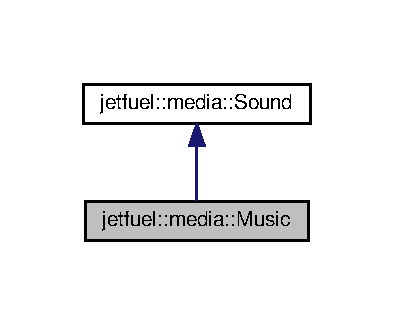
\includegraphics[width=189pt]{classjetfuel_1_1media_1_1Music__inherit__graph}
\end{center}
\end{figure}


Collaboration diagram for jetfuel\+:\+:media\+:\+:Music\+:\nopagebreak
\begin{figure}[H]
\begin{center}
\leavevmode
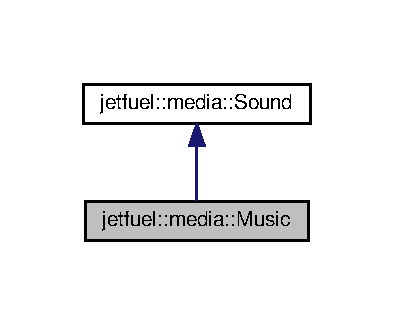
\includegraphics[width=189pt]{classjetfuel_1_1media_1_1Music__coll__graph}
\end{center}
\end{figure}
\subsection*{Public Member Functions}
\begin{DoxyCompactItemize}
\item 
\hyperlink{classjetfuel_1_1media_1_1Music_aa3adce621c89ea9915bd6d13648ac5de}{Music} ()
\begin{DoxyCompactList}\small\item\em Default constructor. \end{DoxyCompactList}\item 
bool \hyperlink{classjetfuel_1_1media_1_1Music_ad19f7983782f39f70e354796c2ba0bd1}{Is\+\_\+music\+\_\+playing} ()
\begin{DoxyCompactList}\small\item\em Returns whether A\+NY music is playing, does not have to be this \hyperlink{classjetfuel_1_1media_1_1Music}{Music} object playing. \end{DoxyCompactList}\item 
bool \hyperlink{classjetfuel_1_1media_1_1Music_a7ed42b22f467dbcdd8d09da9cff5b034}{Is\+\_\+music\+\_\+paused} () const
\begin{DoxyCompactList}\small\item\em Returns whether this music is paused. \end{DoxyCompactList}\item 
std\+::string \hyperlink{classjetfuel_1_1media_1_1Music_a157b382df9640e2df504de9ed1beb031}{Get\+\_\+loaded\+\_\+music\+\_\+file\+\_\+path} () const
\begin{DoxyCompactList}\small\item\em Gets the loaded music\textquotesingle{}s file path. \end{DoxyCompactList}\item 
bool \hyperlink{classjetfuel_1_1media_1_1Music_ae24079b0301f5cf845d094e32ed22da1}{Load\+\_\+audio\+\_\+file} (const std\+::string musicfilepath) override
\begin{DoxyCompactList}\small\item\em Loads an audio music file. \end{DoxyCompactList}\item 
bool \hyperlink{classjetfuel_1_1media_1_1Music_afe9abee662a68ea9391e94e37c79945e}{Play} () override
\begin{DoxyCompactList}\small\item\em Plays the music from the loaded audio file and returns if it succeeded starting playback. \end{DoxyCompactList}\item 
void \hyperlink{classjetfuel_1_1media_1_1Music_a002f31a60671c229bd054539caf537c5}{Pause} () override
\begin{DoxyCompactList}\small\item\em Pauses the music playback. \end{DoxyCompactList}\item 
void \hyperlink{classjetfuel_1_1media_1_1Music_a0c8e12634e29cfe37138349776b6d9a8}{Resume} () override
\begin{DoxyCompactList}\small\item\em Resumes the music playback after it was paused. \end{DoxyCompactList}\end{DoxyCompactItemize}
\subsection*{Protected Member Functions}
\begin{DoxyCompactItemize}
\item 
bool \hyperlink{classjetfuel_1_1media_1_1Music_ac665232356b8b316790e46a3423c158a}{Is\+\_\+music\+\_\+loaded} () const
\begin{DoxyCompactList}\small\item\em Returns whether this \hyperlink{classjetfuel_1_1media_1_1Music}{Music}\textquotesingle{}s audio file is loaded. \end{DoxyCompactList}\item 
bool \hyperlink{classjetfuel_1_1media_1_1Music_a298ce99e6d22e199d1642c21fd18a672}{Play\+\_\+music} ()
\begin{DoxyCompactList}\small\item\em Plays this \hyperlink{classjetfuel_1_1media_1_1Music}{Music}\textquotesingle{}s audio file. \end{DoxyCompactList}\item 
void \hyperlink{classjetfuel_1_1media_1_1Music_a16f346ddd22ce93c347f53f2f930d3fe}{Pause\+\_\+music} ()
\begin{DoxyCompactList}\small\item\em Pauses the music. \end{DoxyCompactList}\item 
void \hyperlink{classjetfuel_1_1media_1_1Music_a390925626dcd2531d1b287f0bfb401fd}{Resume\+\_\+music} ()
\begin{DoxyCompactList}\small\item\em Resumes the music. \end{DoxyCompactList}\end{DoxyCompactItemize}


\subsection{Detailed Description}
A sound playback class for long audio files (example\+: B\+GM), which supports W\+AV(.wav), A\+I\+FF(.aiff), V\+OC(.voc), M\+OD(.mod, .xm, .s3m, and more), M\+I\+DI(.mid), Ogg\+Vorbis(.ogg), M\+P3(.mp3), and F\+L\+AC(.flac).

Code Example\+: 
\begin{DoxyCode}
\hyperlink{classjetfuel_1_1media_1_1Music}{jetfuel::media::Music} music;

\textcolor{keywordflow}{if}(music.load\_audio\_file(\textcolor{stringliteral}{"BGM.ogg"}))\{
    std::cout << \textcolor{stringliteral}{"Unable to load BGM.ogg Error:"} << Mix\_GetError() 
    << \hyperlink{namespacestd}{std}:endl;
    \textcolor{keywordflow}{return} 1;
\}

music.\hyperlink{classjetfuel_1_1media_1_1Music_afe9abee662a68ea9391e94e37c79945e}{Play}();
\end{DoxyCode}
 

\subsection{Constructor \& Destructor Documentation}
\mbox{\Hypertarget{classjetfuel_1_1media_1_1Music_aa3adce621c89ea9915bd6d13648ac5de}\label{classjetfuel_1_1media_1_1Music_aa3adce621c89ea9915bd6d13648ac5de}} 
\index{jetfuel\+::media\+::\+Music@{jetfuel\+::media\+::\+Music}!Music@{Music}}
\index{Music@{Music}!jetfuel\+::media\+::\+Music@{jetfuel\+::media\+::\+Music}}
\subsubsection{\texorpdfstring{Music()}{Music()}}
{\footnotesize\ttfamily jetfuel\+::media\+::\+Music\+::\+Music (\begin{DoxyParamCaption}{ }\end{DoxyParamCaption})}



Default constructor. 

Default constructor. 

\subsection{Member Function Documentation}
\mbox{\Hypertarget{classjetfuel_1_1media_1_1Music_a157b382df9640e2df504de9ed1beb031}\label{classjetfuel_1_1media_1_1Music_a157b382df9640e2df504de9ed1beb031}} 
\index{jetfuel\+::media\+::\+Music@{jetfuel\+::media\+::\+Music}!Get\+\_\+loaded\+\_\+music\+\_\+file\+\_\+path@{Get\+\_\+loaded\+\_\+music\+\_\+file\+\_\+path}}
\index{Get\+\_\+loaded\+\_\+music\+\_\+file\+\_\+path@{Get\+\_\+loaded\+\_\+music\+\_\+file\+\_\+path}!jetfuel\+::media\+::\+Music@{jetfuel\+::media\+::\+Music}}
\subsubsection{\texorpdfstring{Get\+\_\+loaded\+\_\+music\+\_\+file\+\_\+path()}{Get\_loaded\_music\_file\_path()}}
{\footnotesize\ttfamily std\+::string jetfuel\+::media\+::\+Music\+::\+Get\+\_\+loaded\+\_\+music\+\_\+file\+\_\+path (\begin{DoxyParamCaption}{ }\end{DoxyParamCaption}) const\hspace{0.3cm}{\ttfamily [inline]}}



Gets the loaded music\textquotesingle{}s file path. 

Gets the loaded music\textquotesingle{}s file path. \mbox{\Hypertarget{classjetfuel_1_1media_1_1Music_ac665232356b8b316790e46a3423c158a}\label{classjetfuel_1_1media_1_1Music_ac665232356b8b316790e46a3423c158a}} 
\index{jetfuel\+::media\+::\+Music@{jetfuel\+::media\+::\+Music}!Is\+\_\+music\+\_\+loaded@{Is\+\_\+music\+\_\+loaded}}
\index{Is\+\_\+music\+\_\+loaded@{Is\+\_\+music\+\_\+loaded}!jetfuel\+::media\+::\+Music@{jetfuel\+::media\+::\+Music}}
\subsubsection{\texorpdfstring{Is\+\_\+music\+\_\+loaded()}{Is\_music\_loaded()}}
{\footnotesize\ttfamily bool jetfuel\+::media\+::\+Music\+::\+Is\+\_\+music\+\_\+loaded (\begin{DoxyParamCaption}{ }\end{DoxyParamCaption}) const\hspace{0.3cm}{\ttfamily [inline]}, {\ttfamily [protected]}}



Returns whether this \hyperlink{classjetfuel_1_1media_1_1Music}{Music}\textquotesingle{}s audio file is loaded. 

Returns whether this \hyperlink{classjetfuel_1_1media_1_1Music}{Music}\textquotesingle{}s audio file is loaded. \mbox{\Hypertarget{classjetfuel_1_1media_1_1Music_a7ed42b22f467dbcdd8d09da9cff5b034}\label{classjetfuel_1_1media_1_1Music_a7ed42b22f467dbcdd8d09da9cff5b034}} 
\index{jetfuel\+::media\+::\+Music@{jetfuel\+::media\+::\+Music}!Is\+\_\+music\+\_\+paused@{Is\+\_\+music\+\_\+paused}}
\index{Is\+\_\+music\+\_\+paused@{Is\+\_\+music\+\_\+paused}!jetfuel\+::media\+::\+Music@{jetfuel\+::media\+::\+Music}}
\subsubsection{\texorpdfstring{Is\+\_\+music\+\_\+paused()}{Is\_music\_paused()}}
{\footnotesize\ttfamily bool jetfuel\+::media\+::\+Music\+::\+Is\+\_\+music\+\_\+paused (\begin{DoxyParamCaption}{ }\end{DoxyParamCaption}) const\hspace{0.3cm}{\ttfamily [inline]}}



Returns whether this music is paused. 

Returns whether this music is paused. \mbox{\Hypertarget{classjetfuel_1_1media_1_1Music_ad19f7983782f39f70e354796c2ba0bd1}\label{classjetfuel_1_1media_1_1Music_ad19f7983782f39f70e354796c2ba0bd1}} 
\index{jetfuel\+::media\+::\+Music@{jetfuel\+::media\+::\+Music}!Is\+\_\+music\+\_\+playing@{Is\+\_\+music\+\_\+playing}}
\index{Is\+\_\+music\+\_\+playing@{Is\+\_\+music\+\_\+playing}!jetfuel\+::media\+::\+Music@{jetfuel\+::media\+::\+Music}}
\subsubsection{\texorpdfstring{Is\+\_\+music\+\_\+playing()}{Is\_music\_playing()}}
{\footnotesize\ttfamily bool jetfuel\+::media\+::\+Music\+::\+Is\+\_\+music\+\_\+playing (\begin{DoxyParamCaption}{ }\end{DoxyParamCaption})\hspace{0.3cm}{\ttfamily [inline]}}



Returns whether A\+NY music is playing, does not have to be this \hyperlink{classjetfuel_1_1media_1_1Music}{Music} object playing. 

Returns whether A\+NY music is playing, does not have to be this \hyperlink{classjetfuel_1_1media_1_1Music}{Music} object playing. \mbox{\Hypertarget{classjetfuel_1_1media_1_1Music_ae24079b0301f5cf845d094e32ed22da1}\label{classjetfuel_1_1media_1_1Music_ae24079b0301f5cf845d094e32ed22da1}} 
\index{jetfuel\+::media\+::\+Music@{jetfuel\+::media\+::\+Music}!Load\+\_\+audio\+\_\+file@{Load\+\_\+audio\+\_\+file}}
\index{Load\+\_\+audio\+\_\+file@{Load\+\_\+audio\+\_\+file}!jetfuel\+::media\+::\+Music@{jetfuel\+::media\+::\+Music}}
\subsubsection{\texorpdfstring{Load\+\_\+audio\+\_\+file()}{Load\_audio\_file()}}
{\footnotesize\ttfamily bool jetfuel\+::media\+::\+Music\+::\+Load\+\_\+audio\+\_\+file (\begin{DoxyParamCaption}\item[{const std\+::string}]{musicfilepath }\end{DoxyParamCaption})\hspace{0.3cm}{\ttfamily [inline]}, {\ttfamily [override]}, {\ttfamily [virtual]}}



Loads an audio music file. 

Loads an audio music file.


\begin{DoxyParams}{Parameters}
{\em std\+::string} & musicfilepath \\
\hline
\end{DoxyParams}


Implements \hyperlink{classjetfuel_1_1media_1_1Sound_ab18ff9b8dd2001fa11b17649a6a3defb}{jetfuel\+::media\+::\+Sound}.

\mbox{\Hypertarget{classjetfuel_1_1media_1_1Music_a002f31a60671c229bd054539caf537c5}\label{classjetfuel_1_1media_1_1Music_a002f31a60671c229bd054539caf537c5}} 
\index{jetfuel\+::media\+::\+Music@{jetfuel\+::media\+::\+Music}!Pause@{Pause}}
\index{Pause@{Pause}!jetfuel\+::media\+::\+Music@{jetfuel\+::media\+::\+Music}}
\subsubsection{\texorpdfstring{Pause()}{Pause()}}
{\footnotesize\ttfamily void jetfuel\+::media\+::\+Music\+::\+Pause (\begin{DoxyParamCaption}{ }\end{DoxyParamCaption})\hspace{0.3cm}{\ttfamily [override]}, {\ttfamily [virtual]}}



Pauses the music playback. 

Pauses the music playback. 

Implements \hyperlink{classjetfuel_1_1media_1_1Sound_adb9cd45e23e6224760051e579aeefa7f}{jetfuel\+::media\+::\+Sound}.

\mbox{\Hypertarget{classjetfuel_1_1media_1_1Music_a16f346ddd22ce93c347f53f2f930d3fe}\label{classjetfuel_1_1media_1_1Music_a16f346ddd22ce93c347f53f2f930d3fe}} 
\index{jetfuel\+::media\+::\+Music@{jetfuel\+::media\+::\+Music}!Pause\+\_\+music@{Pause\+\_\+music}}
\index{Pause\+\_\+music@{Pause\+\_\+music}!jetfuel\+::media\+::\+Music@{jetfuel\+::media\+::\+Music}}
\subsubsection{\texorpdfstring{Pause\+\_\+music()}{Pause\_music()}}
{\footnotesize\ttfamily void jetfuel\+::media\+::\+Music\+::\+Pause\+\_\+music (\begin{DoxyParamCaption}{ }\end{DoxyParamCaption})\hspace{0.3cm}{\ttfamily [inline]}, {\ttfamily [protected]}}



Pauses the music. 

Pauses the music. \mbox{\Hypertarget{classjetfuel_1_1media_1_1Music_afe9abee662a68ea9391e94e37c79945e}\label{classjetfuel_1_1media_1_1Music_afe9abee662a68ea9391e94e37c79945e}} 
\index{jetfuel\+::media\+::\+Music@{jetfuel\+::media\+::\+Music}!Play@{Play}}
\index{Play@{Play}!jetfuel\+::media\+::\+Music@{jetfuel\+::media\+::\+Music}}
\subsubsection{\texorpdfstring{Play()}{Play()}}
{\footnotesize\ttfamily bool jetfuel\+::media\+::\+Music\+::\+Play (\begin{DoxyParamCaption}{ }\end{DoxyParamCaption})\hspace{0.3cm}{\ttfamily [override]}, {\ttfamily [virtual]}}



Plays the music from the loaded audio file and returns if it succeeded starting playback. 

Plays the music from the loaded audio file and returns if it succeeded starting playback. 

Implements \hyperlink{classjetfuel_1_1media_1_1Sound_a8861a6671ce039522179d61085f240c8}{jetfuel\+::media\+::\+Sound}.

\mbox{\Hypertarget{classjetfuel_1_1media_1_1Music_a298ce99e6d22e199d1642c21fd18a672}\label{classjetfuel_1_1media_1_1Music_a298ce99e6d22e199d1642c21fd18a672}} 
\index{jetfuel\+::media\+::\+Music@{jetfuel\+::media\+::\+Music}!Play\+\_\+music@{Play\+\_\+music}}
\index{Play\+\_\+music@{Play\+\_\+music}!jetfuel\+::media\+::\+Music@{jetfuel\+::media\+::\+Music}}
\subsubsection{\texorpdfstring{Play\+\_\+music()}{Play\_music()}}
{\footnotesize\ttfamily bool jetfuel\+::media\+::\+Music\+::\+Play\+\_\+music (\begin{DoxyParamCaption}{ }\end{DoxyParamCaption})\hspace{0.3cm}{\ttfamily [inline]}, {\ttfamily [protected]}}



Plays this \hyperlink{classjetfuel_1_1media_1_1Music}{Music}\textquotesingle{}s audio file. 

Plays this \hyperlink{classjetfuel_1_1media_1_1Music}{Music}\textquotesingle{}s audio file. \mbox{\Hypertarget{classjetfuel_1_1media_1_1Music_a0c8e12634e29cfe37138349776b6d9a8}\label{classjetfuel_1_1media_1_1Music_a0c8e12634e29cfe37138349776b6d9a8}} 
\index{jetfuel\+::media\+::\+Music@{jetfuel\+::media\+::\+Music}!Resume@{Resume}}
\index{Resume@{Resume}!jetfuel\+::media\+::\+Music@{jetfuel\+::media\+::\+Music}}
\subsubsection{\texorpdfstring{Resume()}{Resume()}}
{\footnotesize\ttfamily void jetfuel\+::media\+::\+Music\+::\+Resume (\begin{DoxyParamCaption}{ }\end{DoxyParamCaption})\hspace{0.3cm}{\ttfamily [override]}, {\ttfamily [virtual]}}



Resumes the music playback after it was paused. 

Resumes the music playback after it was paused. 

Implements \hyperlink{classjetfuel_1_1media_1_1Sound_af781fccd8ebb1305e97dc8f6b7c828dc}{jetfuel\+::media\+::\+Sound}.

\mbox{\Hypertarget{classjetfuel_1_1media_1_1Music_a390925626dcd2531d1b287f0bfb401fd}\label{classjetfuel_1_1media_1_1Music_a390925626dcd2531d1b287f0bfb401fd}} 
\index{jetfuel\+::media\+::\+Music@{jetfuel\+::media\+::\+Music}!Resume\+\_\+music@{Resume\+\_\+music}}
\index{Resume\+\_\+music@{Resume\+\_\+music}!jetfuel\+::media\+::\+Music@{jetfuel\+::media\+::\+Music}}
\subsubsection{\texorpdfstring{Resume\+\_\+music()}{Resume\_music()}}
{\footnotesize\ttfamily void jetfuel\+::media\+::\+Music\+::\+Resume\+\_\+music (\begin{DoxyParamCaption}{ }\end{DoxyParamCaption})\hspace{0.3cm}{\ttfamily [inline]}, {\ttfamily [protected]}}



Resumes the music. 

Resumes the music. 

The documentation for this class was generated from the following file\+:\begin{DoxyCompactItemize}
\item 
include/jetfuelmedia/music.\+h\end{DoxyCompactItemize}

\hypertarget{classjetfuel_1_1draw_1_1exceptions_1_1Nullptr__SDL__ttf__exception}{}\section{jetfuel\+:\+:draw\+:\+:exceptions\+:\+:Nullptr\+\_\+\+S\+D\+L\+\_\+ttf\+\_\+exception Class Reference}
\label{classjetfuel_1_1draw_1_1exceptions_1_1Nullptr__SDL__ttf__exception}\index{jetfuel\+::draw\+::exceptions\+::\+Nullptr\+\_\+\+S\+D\+L\+\_\+ttf\+\_\+exception@{jetfuel\+::draw\+::exceptions\+::\+Nullptr\+\_\+\+S\+D\+L\+\_\+ttf\+\_\+exception}}


{\ttfamily \#include $<$text.\+h$>$}



Inheritance diagram for jetfuel\+:\+:draw\+:\+:exceptions\+:\+:Nullptr\+\_\+\+S\+D\+L\+\_\+ttf\+\_\+exception\+:
\nopagebreak
\begin{figure}[H]
\begin{center}
\leavevmode
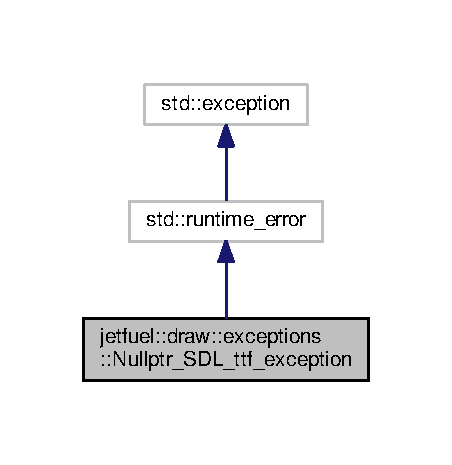
\includegraphics[width=217pt]{classjetfuel_1_1draw_1_1exceptions_1_1Nullptr__SDL__ttf__exception__inherit__graph}
\end{center}
\end{figure}


Collaboration diagram for jetfuel\+:\+:draw\+:\+:exceptions\+:\+:Nullptr\+\_\+\+S\+D\+L\+\_\+ttf\+\_\+exception\+:
\nopagebreak
\begin{figure}[H]
\begin{center}
\leavevmode
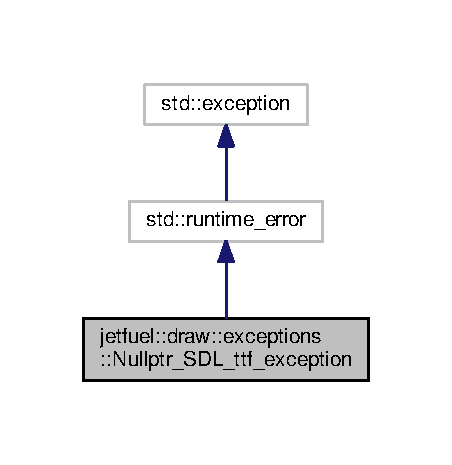
\includegraphics[width=217pt]{classjetfuel_1_1draw_1_1exceptions_1_1Nullptr__SDL__ttf__exception__coll__graph}
\end{center}
\end{figure}
\subsection*{Public Member Functions}
\begin{DoxyCompactItemize}
\item 
\hyperlink{classjetfuel_1_1draw_1_1exceptions_1_1Nullptr__SDL__ttf__exception_ac6644eee07afa5a2f8a972f98905f250}{Nullptr\+\_\+\+S\+D\+L\+\_\+ttf\+\_\+exception} ()
\begin{DoxyCompactList}\small\item\em Constructs a \hyperlink{classjetfuel_1_1draw_1_1exceptions_1_1Nullptr__SDL__ttf__exception}{Nullptr\+\_\+\+S\+D\+L\+\_\+ttf\+\_\+exception}. \end{DoxyCompactList}\end{DoxyCompactItemize}


\subsection{Detailed Description}
\hyperlink{classjetfuel_1_1draw_1_1exceptions_1_1Font__not__init__exception}{jetfuel\+::draw\+::exceptions\+::\+Font\+\_\+not\+\_\+init\+\_\+exception}

This exception should be thrown when a font passed into a function as an argument is not loaded and ready for the class to use it. This exception is not meant to be used outside of the \hyperlink{classjetfuel_1_1draw_1_1Text}{Text} class.

Code Example\+:

void Do\+\_\+something\+\_\+with\+\_\+font(\+Font font)\{ if(font.\+Is\+\_\+font\+\_\+loaded())\{ // do something with the font... \}else\{ throw jetfuel\+::draw\+::exceptions\+:\+: Font\+\_\+not\+\_\+init\+\_\+exception(); \} \} 

\subsection{Constructor \& Destructor Documentation}
\mbox{\Hypertarget{classjetfuel_1_1draw_1_1exceptions_1_1Nullptr__SDL__ttf__exception_ac6644eee07afa5a2f8a972f98905f250}\label{classjetfuel_1_1draw_1_1exceptions_1_1Nullptr__SDL__ttf__exception_ac6644eee07afa5a2f8a972f98905f250}} 
\index{jetfuel\+::draw\+::exceptions\+::\+Nullptr\+\_\+\+S\+D\+L\+\_\+ttf\+\_\+exception@{jetfuel\+::draw\+::exceptions\+::\+Nullptr\+\_\+\+S\+D\+L\+\_\+ttf\+\_\+exception}!Nullptr\+\_\+\+S\+D\+L\+\_\+ttf\+\_\+exception@{Nullptr\+\_\+\+S\+D\+L\+\_\+ttf\+\_\+exception}}
\index{Nullptr\+\_\+\+S\+D\+L\+\_\+ttf\+\_\+exception@{Nullptr\+\_\+\+S\+D\+L\+\_\+ttf\+\_\+exception}!jetfuel\+::draw\+::exceptions\+::\+Nullptr\+\_\+\+S\+D\+L\+\_\+ttf\+\_\+exception@{jetfuel\+::draw\+::exceptions\+::\+Nullptr\+\_\+\+S\+D\+L\+\_\+ttf\+\_\+exception}}
\subsubsection{\texorpdfstring{Nullptr\+\_\+\+S\+D\+L\+\_\+ttf\+\_\+exception()}{Nullptr\_SDL\_ttf\_exception()}}
{\footnotesize\ttfamily jetfuel\+::draw\+::exceptions\+::\+Nullptr\+\_\+\+S\+D\+L\+\_\+ttf\+\_\+exception\+::\+Nullptr\+\_\+\+S\+D\+L\+\_\+ttf\+\_\+exception (\begin{DoxyParamCaption}{ }\end{DoxyParamCaption})\hspace{0.3cm}{\ttfamily [inline]}}



Constructs a \hyperlink{classjetfuel_1_1draw_1_1exceptions_1_1Nullptr__SDL__ttf__exception}{Nullptr\+\_\+\+S\+D\+L\+\_\+ttf\+\_\+exception}. 

Constructs a \hyperlink{classjetfuel_1_1draw_1_1exceptions_1_1Nullptr__SDL__ttf__exception}{Nullptr\+\_\+\+S\+D\+L\+\_\+ttf\+\_\+exception}. 

The documentation for this class was generated from the following file\+:\begin{DoxyCompactItemize}
\item 
include/jetfueldraw/text.\+h\end{DoxyCompactItemize}

\hypertarget{classjetfuel_1_1core_1_1exceptions_1_1Out__of__vector__range__exception}{}\section{jetfuel\+:\+:core\+:\+:exceptions\+:\+:Out\+\_\+of\+\_\+vector\+\_\+range\+\_\+exception Class Reference}
\label{classjetfuel_1_1core_1_1exceptions_1_1Out__of__vector__range__exception}\index{jetfuel\+::core\+::exceptions\+::\+Out\+\_\+of\+\_\+vector\+\_\+range\+\_\+exception@{jetfuel\+::core\+::exceptions\+::\+Out\+\_\+of\+\_\+vector\+\_\+range\+\_\+exception}}


{\ttfamily \#include $<$messagebus.\+h$>$}



Inheritance diagram for jetfuel\+:\+:core\+:\+:exceptions\+:\+:Out\+\_\+of\+\_\+vector\+\_\+range\+\_\+exception\+:\nopagebreak
\begin{figure}[H]
\begin{center}
\leavevmode
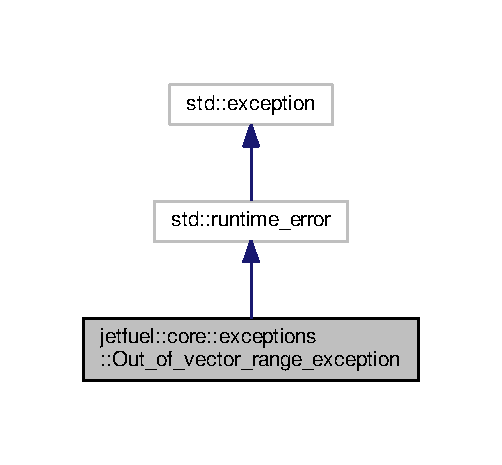
\includegraphics[width=241pt]{classjetfuel_1_1core_1_1exceptions_1_1Out__of__vector__range__exception__inherit__graph}
\end{center}
\end{figure}


Collaboration diagram for jetfuel\+:\+:core\+:\+:exceptions\+:\+:Out\+\_\+of\+\_\+vector\+\_\+range\+\_\+exception\+:\nopagebreak
\begin{figure}[H]
\begin{center}
\leavevmode
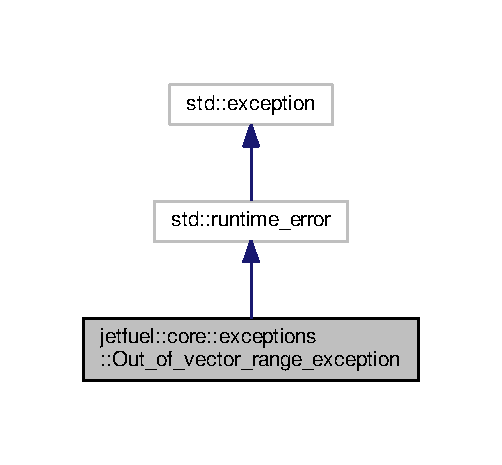
\includegraphics[width=241pt]{classjetfuel_1_1core_1_1exceptions_1_1Out__of__vector__range__exception__coll__graph}
\end{center}
\end{figure}


\subsection{Detailed Description}
This exception is thrown when a function requests for data from a vector location that is outside of that vector\textquotesingle{}s range.

Code Example\+: 
\begin{DoxyCode}
\textcolor{keywordtype}{int} Get\_int\_in\_vector(\textcolor{keyword}{const} \textcolor{keywordtype}{int} location)\textcolor{keyword}{ const }\{
    \textcolor{keywordflow}{if}(intvector.size() <= location)\{
        \textcolor{keywordflow}{throw} exceptions::Out\_of\_vector\_range\_exception();
    \}\textcolor{keywordflow}{else}\{
        \textcolor{keywordflow}{return} intvector[location];
    \}
\}
\end{DoxyCode}
 

The documentation for this class was generated from the following file\+:\begin{DoxyCompactItemize}
\item 
include/jetfuelcore/messagebus.\+h\end{DoxyCompactItemize}

\hypertarget{classjetfuel_1_1inspire_1_1Pointer__bridge}{}\section{jetfuel\+:\+:inspire\+:\+:Pointer\+\_\+bridge Class Reference}
\label{classjetfuel_1_1inspire_1_1Pointer__bridge}\index{jetfuel\+::inspire\+::\+Pointer\+\_\+bridge@{jetfuel\+::inspire\+::\+Pointer\+\_\+bridge}}


{\ttfamily \#include $<$pointerbridge.\+h$>$}

\subsection*{Public Member Functions}
\begin{DoxyCompactItemize}
\item 
\hyperlink{classjetfuel_1_1inspire_1_1Pointer__bridge_a8b799f891596d70d98ee577ef87a6781}{Pointer\+\_\+bridge} ()
\begin{DoxyCompactList}\small\item\em Default constructor. \end{DoxyCompactList}\item 
void $\ast$ \hyperlink{classjetfuel_1_1inspire_1_1Pointer__bridge_a031c7d904e4e86096e2c399f8db8a1f8}{Recieve\+\_\+pointer} (std\+::string id, bool $\ast$found)
\begin{DoxyCompactList}\small\item\em Recieves a pointer sent with an id (of the pointer) and a pointer pointing to a boolean variable whether the pointer has been recieved. \end{DoxyCompactList}\item 
void \hyperlink{classjetfuel_1_1inspire_1_1Pointer__bridge_a805c0fa469cca7d6acdfd285b92aa9c8}{Send\+\_\+pointer} (std\+::string id, void $\ast$pointer)
\begin{DoxyCompactList}\small\item\em Sends a pointer with an id identifying that pointer. \end{DoxyCompactList}\end{DoxyCompactItemize}


\subsection{Detailed Description}
A simple pointer bridge meant for sending pointers between Python and C++ for object mainuplations.

Code Example\+:

Python(main.\+py)\+:

def main(pointerbridgeref)\+: if(system() == \char`\"{}\+Windows\char`\"{})\+: jetfuelpythonapiso = abspath(\char`\"{}\+Python\+A\+P\+I.\+dll\char`\"{}); else\+: jetfuelpythonapiso = abspath( \char`\"{}lib\+Jetfuel Game Engine Python A\+P\+I.\+so\char`\"{}); jetfuelso = jetfuelsoloader(jetfuelpythonapiso); pointerbridge = pointer\+\_\+bridge(jetfuelpythonapiso, pointerbridgeref); found = True; scenemanager = pointerbridge.\+recieve\+\_\+pointer(\char`\"{}scenemanager\char`\"{}, found); if(found)\+: print(\char`\"{}\+Got scenemanager pointer! It is\+:\char`\"{}+ hex(scenemanager.\+scenemanagerref)); else\+: print(\char`\"{}\+Could not get scenemanager pointer!\char`\"{});

C++\+: \hyperlink{classjetfuel_1_1draw_1_1Scene__manager}{jetfuel\+::draw\+::\+Scene\+\_\+manager} scenemanager; \hyperlink{classjetfuel_1_1inspire_1_1Python__module__loader}{jetfuel\+::inspire\+::\+Python\+\_\+module\+\_\+loader} module(\char`\"{}main.\+py\char`\"{}, \char`\"{}main\char`\"{}); \hyperlink{classjetfuel_1_1inspire_1_1Pointer__bridge}{jetfuel\+::inspire\+::\+Pointer\+\_\+bridge} $\ast$bridge = new \hyperlink{classjetfuel_1_1inspire_1_1Pointer__bridge}{jetfuel\+::inspire\+::\+Pointer\+\_\+bridge()}; std\+::string error; bool executed = true;

bridge.\+send\+\_\+pointer(\char`\"{}scenemanager\char`\"{}, \&scenemanager);

Py\+Object $\ast$args = Py\+Tuple\+\_\+\+Pack(1, Py\+Long\+\_\+\+From\+Long( reinterpret\+\_\+cast$<$long int$>$(scenemanager)));

module.\+Execute(\&executed, \&error, args);

if(!executed)\{ std\+::cout $<$$<$ \char`\"{}\+Python Error occured! Error was\+:\char`\"{} $<$$<$ error $<$$<$ std\+::endl; 

\subsection{Constructor \& Destructor Documentation}
\mbox{\Hypertarget{classjetfuel_1_1inspire_1_1Pointer__bridge_a8b799f891596d70d98ee577ef87a6781}\label{classjetfuel_1_1inspire_1_1Pointer__bridge_a8b799f891596d70d98ee577ef87a6781}} 
\index{jetfuel\+::inspire\+::\+Pointer\+\_\+bridge@{jetfuel\+::inspire\+::\+Pointer\+\_\+bridge}!Pointer\+\_\+bridge@{Pointer\+\_\+bridge}}
\index{Pointer\+\_\+bridge@{Pointer\+\_\+bridge}!jetfuel\+::inspire\+::\+Pointer\+\_\+bridge@{jetfuel\+::inspire\+::\+Pointer\+\_\+bridge}}
\subsubsection{\texorpdfstring{Pointer\+\_\+bridge()}{Pointer\_bridge()}}
{\footnotesize\ttfamily jetfuel\+::inspire\+::\+Pointer\+\_\+bridge\+::\+Pointer\+\_\+bridge (\begin{DoxyParamCaption}{ }\end{DoxyParamCaption})\hspace{0.3cm}{\ttfamily [inline]}}



Default constructor. 

Default constructor. 

\subsection{Member Function Documentation}
\mbox{\Hypertarget{classjetfuel_1_1inspire_1_1Pointer__bridge_a031c7d904e4e86096e2c399f8db8a1f8}\label{classjetfuel_1_1inspire_1_1Pointer__bridge_a031c7d904e4e86096e2c399f8db8a1f8}} 
\index{jetfuel\+::inspire\+::\+Pointer\+\_\+bridge@{jetfuel\+::inspire\+::\+Pointer\+\_\+bridge}!Recieve\+\_\+pointer@{Recieve\+\_\+pointer}}
\index{Recieve\+\_\+pointer@{Recieve\+\_\+pointer}!jetfuel\+::inspire\+::\+Pointer\+\_\+bridge@{jetfuel\+::inspire\+::\+Pointer\+\_\+bridge}}
\subsubsection{\texorpdfstring{Recieve\+\_\+pointer()}{Recieve\_pointer()}}
{\footnotesize\ttfamily void$\ast$ jetfuel\+::inspire\+::\+Pointer\+\_\+bridge\+::\+Recieve\+\_\+pointer (\begin{DoxyParamCaption}\item[{std\+::string}]{id,  }\item[{bool $\ast$}]{found }\end{DoxyParamCaption})\hspace{0.3cm}{\ttfamily [inline]}}



Recieves a pointer sent with an id (of the pointer) and a pointer pointing to a boolean variable whether the pointer has been recieved. 

Recieves a pointer sent with an id (of the pointer) and a pointer pointing to a boolean variable whether the pointer has been recieved.


\begin{DoxyParams}{Parameters}
{\em std\+::string} & id \\
\hline
{\em bool} & $\ast$found \\
\hline
\end{DoxyParams}
\mbox{\Hypertarget{classjetfuel_1_1inspire_1_1Pointer__bridge_a805c0fa469cca7d6acdfd285b92aa9c8}\label{classjetfuel_1_1inspire_1_1Pointer__bridge_a805c0fa469cca7d6acdfd285b92aa9c8}} 
\index{jetfuel\+::inspire\+::\+Pointer\+\_\+bridge@{jetfuel\+::inspire\+::\+Pointer\+\_\+bridge}!Send\+\_\+pointer@{Send\+\_\+pointer}}
\index{Send\+\_\+pointer@{Send\+\_\+pointer}!jetfuel\+::inspire\+::\+Pointer\+\_\+bridge@{jetfuel\+::inspire\+::\+Pointer\+\_\+bridge}}
\subsubsection{\texorpdfstring{Send\+\_\+pointer()}{Send\_pointer()}}
{\footnotesize\ttfamily void jetfuel\+::inspire\+::\+Pointer\+\_\+bridge\+::\+Send\+\_\+pointer (\begin{DoxyParamCaption}\item[{std\+::string}]{id,  }\item[{void $\ast$}]{pointer }\end{DoxyParamCaption})\hspace{0.3cm}{\ttfamily [inline]}}



Sends a pointer with an id identifying that pointer. 

Sends a pointer with an id identifying that pointer.


\begin{DoxyParams}{Parameters}
{\em std\+::string} & id \\
\hline
{\em void} & $\ast$pointer \\
\hline
\end{DoxyParams}


The documentation for this class was generated from the following file\+:\begin{DoxyCompactItemize}
\item 
include/jetfuelinspire/pointerbridge.\+h\end{DoxyCompactItemize}

\hypertarget{classjetfuel_1_1gui_1_1Progress__bar}{}\section{jetfuel\+:\+:gui\+:\+:Progress\+\_\+bar Class Reference}
\label{classjetfuel_1_1gui_1_1Progress__bar}\index{jetfuel\+::gui\+::\+Progress\+\_\+bar@{jetfuel\+::gui\+::\+Progress\+\_\+bar}}


{\ttfamily \#include $<$progressbar.\+h$>$}



Inheritance diagram for jetfuel\+:\+:gui\+:\+:Progress\+\_\+bar\+:\nopagebreak
\begin{figure}[H]
\begin{center}
\leavevmode
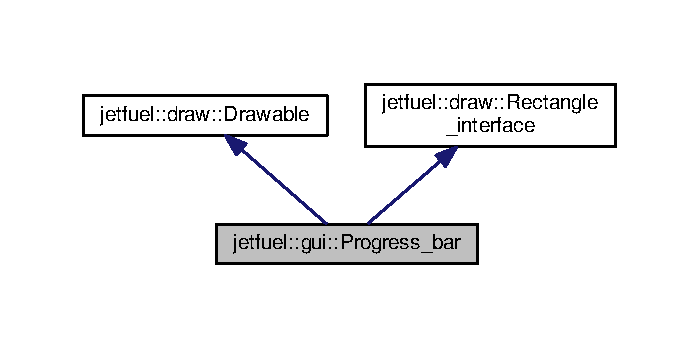
\includegraphics[width=336pt]{classjetfuel_1_1gui_1_1Progress__bar__inherit__graph}
\end{center}
\end{figure}


Collaboration diagram for jetfuel\+:\+:gui\+:\+:Progress\+\_\+bar\+:\nopagebreak
\begin{figure}[H]
\begin{center}
\leavevmode
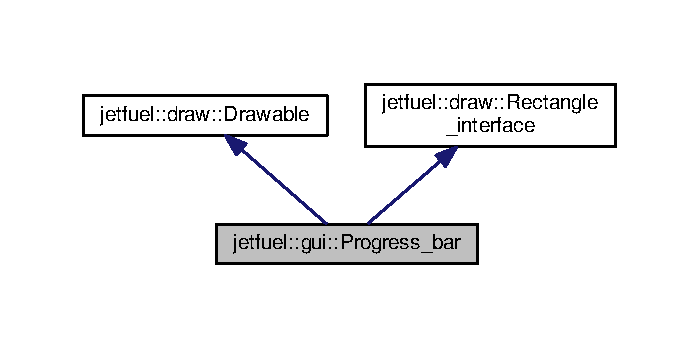
\includegraphics[width=336pt]{classjetfuel_1_1gui_1_1Progress__bar__coll__graph}
\end{center}
\end{figure}
\subsection*{Public Member Functions}
\begin{DoxyCompactItemize}
\item 
\hyperlink{classjetfuel_1_1gui_1_1Progress__bar_a82ff3b06366efe839c6031281db9b9ac}{Progress\+\_\+bar} ()
\begin{DoxyCompactList}\small\item\em Default Constructor. \end{DoxyCompactList}\item 
\hyperlink{classjetfuel_1_1gui_1_1Progress__bar_a77c734bd7d04bd5f8a0f9bf6d2c600e5}{Progress\+\_\+bar} (const \hyperlink{classjetfuel_1_1draw_1_1Image}{jetfuel\+::draw\+::\+Image} progressbarholderimage, const \hyperlink{classjetfuel_1_1draw_1_1Color}{jetfuel\+::draw\+::\+Color} progressbarcolor, const \hyperlink{classjetfuel_1_1draw_1_1Rect2d}{jetfuel\+::draw\+::\+Rect2d\+\_\+int} progressbarholderborders, const unsigned int progressbarmax=100)
\begin{DoxyCompactList}\small\item\em Constructs a \hyperlink{classjetfuel_1_1gui_1_1Progress__bar}{Progress\+\_\+bar} with a holder image, a color (for the bar), the borders of the holder image, and the max number of this \hyperlink{classjetfuel_1_1gui_1_1Progress__bar}{Progress\+\_\+bar}\textquotesingle{}s progress. \end{DoxyCompactList}\item 
void \hyperlink{classjetfuel_1_1gui_1_1Progress__bar_aef1b768b22c17ce9dab2fd12a9370262}{Set\+\_\+progress\+\_\+bar} (const \hyperlink{classjetfuel_1_1draw_1_1Image}{jetfuel\+::draw\+::\+Image} progressbarholderimage, const \hyperlink{classjetfuel_1_1draw_1_1Color}{jetfuel\+::draw\+::\+Color} progressbarcolor, const \hyperlink{classjetfuel_1_1draw_1_1Rect2d}{jetfuel\+::draw\+::\+Rect2d\+\_\+int} progressbarholderborders, const unsigned int progressbarmax=100)
\begin{DoxyCompactList}\small\item\em Sets a \hyperlink{classjetfuel_1_1gui_1_1Progress__bar}{Progress\+\_\+bar} with a holder image, a color (for the bar), the borders of the holder image, and the max number of this \hyperlink{classjetfuel_1_1gui_1_1Progress__bar}{Progress\+\_\+bar}\textquotesingle{}s progress. \end{DoxyCompactList}\item 
unsigned int \hyperlink{classjetfuel_1_1gui_1_1Progress__bar_ae1fc30f6eacefc0fcca909d7d3f52225}{Get\+\_\+progress\+\_\+bar\+\_\+progress} () const
\begin{DoxyCompactList}\small\item\em Gets this \hyperlink{classjetfuel_1_1gui_1_1Progress__bar}{Progress\+\_\+bar}\textquotesingle{}s progress. \end{DoxyCompactList}\item 
void \hyperlink{classjetfuel_1_1gui_1_1Progress__bar_a53343a5c7313be548245b9bac150b223}{Set\+\_\+progress\+\_\+bar\+\_\+progress} (const unsigned int progressbarprogress)
\begin{DoxyCompactList}\small\item\em Sets this \hyperlink{classjetfuel_1_1gui_1_1Progress__bar}{Progress\+\_\+bar}\textquotesingle{}s progress. \end{DoxyCompactList}\item 
unsigned int \hyperlink{classjetfuel_1_1gui_1_1Progress__bar_a6c9fdfbed3600490da1a9f1fb4a76003}{Get\+\_\+max\+\_\+progress\+\_\+bar} () const
\begin{DoxyCompactList}\small\item\em Gets the max progress bar progress. \end{DoxyCompactList}\item 
bool \hyperlink{classjetfuel_1_1gui_1_1Progress__bar_ab21545ddc2fbd947f1fbe9bdf11b959f}{Has\+\_\+progress\+\_\+bar\+\_\+completed} ()
\begin{DoxyCompactList}\small\item\em Returns whether this \hyperlink{classjetfuel_1_1gui_1_1Progress__bar}{Progress\+\_\+bar} has been completed. \end{DoxyCompactList}\item 
void \hyperlink{classjetfuel_1_1gui_1_1Progress__bar_a34797d42cedf5ff096eafb58c2e76128}{Assign\+\_\+renderer} (S\+D\+L\+\_\+\+Renderer $\ast$renderer) override
\begin{DoxyCompactList}\small\item\em Assigns a S\+DL Renderer to this \hyperlink{classjetfuel_1_1gui_1_1Progress__bar}{Progress\+\_\+bar}\textquotesingle{}s objects. \end{DoxyCompactList}\item 
\hyperlink{classjetfuel_1_1draw_1_1Vector2d}{jetfuel\+::draw\+::\+Vector2d\+\_\+int} \hyperlink{classjetfuel_1_1gui_1_1Progress__bar_a5771ea71b321c173383e89537cea0ae1}{Get\+\_\+position} () override
\begin{DoxyCompactList}\small\item\em Gets this \hyperlink{classjetfuel_1_1gui_1_1Progress__bar}{Progress\+\_\+bar}\textquotesingle{}s position. \end{DoxyCompactList}\item 
void \hyperlink{classjetfuel_1_1gui_1_1Progress__bar_a5f52369cccd805274805abf5913535df}{Set\+\_\+position} (\hyperlink{classjetfuel_1_1draw_1_1Vector2d}{jetfuel\+::draw\+::\+Vector2d\+\_\+int} position) override
\begin{DoxyCompactList}\small\item\em Sets this \hyperlink{classjetfuel_1_1gui_1_1Progress__bar}{Progress\+\_\+bar}\textquotesingle{}s position. \end{DoxyCompactList}\item 
\hyperlink{classjetfuel_1_1draw_1_1Rect2d}{jetfuel\+::draw\+::\+Rect2d\+\_\+int} \hyperlink{classjetfuel_1_1gui_1_1Progress__bar_a4a09c3d515c9754b8295a4b5d83291ff}{Get\+\_\+rect\+\_\+to\+\_\+draw} () override
\begin{DoxyCompactList}\small\item\em Gets the rect to be drawn when the function Draw is called. \end{DoxyCompactList}\item 
bool \hyperlink{classjetfuel_1_1gui_1_1Progress__bar_a91a7ffe82738105be9b36a48dca1cdec}{Draw} () override
\begin{DoxyCompactList}\small\item\em Draws this \hyperlink{classjetfuel_1_1gui_1_1Progress__bar}{Progress\+\_\+bar}. \end{DoxyCompactList}\end{DoxyCompactItemize}
\subsection*{Protected Member Functions}
\begin{DoxyCompactItemize}
\item 
bool \hyperlink{classjetfuel_1_1gui_1_1Progress__bar_a97bc9fab7b77a271db47f91c95af8672}{Draw\+\_\+progress\+\_\+bar\+\_\+holder} ()
\begin{DoxyCompactList}\small\item\em Draws this \hyperlink{classjetfuel_1_1gui_1_1Progress__bar}{Progress\+\_\+bar}\textquotesingle{}s holder sprite. \end{DoxyCompactList}\item 
bool \hyperlink{classjetfuel_1_1gui_1_1Progress__bar_ad27c8ac735ad8698fce255b642cc6944}{Draw\+\_\+progress\+\_\+bar} ()
\begin{DoxyCompactList}\small\item\em Draws this \hyperlink{classjetfuel_1_1gui_1_1Progress__bar}{Progress\+\_\+bar}\textquotesingle{}s colored rectangle (the actual progress bar). \end{DoxyCompactList}\item 
int \hyperlink{classjetfuel_1_1gui_1_1Progress__bar_ac8399712a5a25311f8f618ed33f730dc}{Get\+\_\+max\+\_\+progress\+\_\+bar\+\_\+width} () const
\begin{DoxyCompactList}\small\item\em Gets the max size of the progress bar (in width). \end{DoxyCompactList}\item 
void \hyperlink{classjetfuel_1_1gui_1_1Progress__bar_a5975a20358c54bc05d87d4285cefe990}{Set\+\_\+width\+\_\+of\+\_\+progress\+\_\+bar} (const int width)
\begin{DoxyCompactList}\small\item\em Sets the width of the progress bar. \end{DoxyCompactList}\item 
void \hyperlink{classjetfuel_1_1gui_1_1Progress__bar_a4871a444df390b3a4996ce8bb67f90c8}{Mark\+\_\+progress\+\_\+bar\+\_\+size} ()
\begin{DoxyCompactList}\small\item\em Forces a refresh of the max size of the progress bar. \end{DoxyCompactList}\end{DoxyCompactItemize}


\subsection{Detailed Description}
A simple progress bar with a holder sprite and a colored rectangle representing the progress bar.

Code Example\+: 
\begin{DoxyCode}
\hyperlink{classjetfuel_1_1draw_1_1Scene__manager}{jetfuel::draw::Scene\_manager} scenemanager;
\hyperlink{classjetfuel_1_1draw_1_1Scene}{jetfuel::draw::Scene} scene1(1);
\hyperlink{classjetfuel_1_1core_1_1Message__bus}{jetfuel::core::Message\_bus} messagebus;
\hyperlink{classjetfuel_1_1draw_1_1Image}{jetfuel::draw::Image} progressbarholderimage(
                                        \textcolor{stringliteral}{"progressbarholder.png"},
                                          &scenemanager);
\hyperlink{classjetfuel_1_1gui_1_1Progress__bar}{jetfuel::gui::Progress\_bar} progressbar(progressbarholderimage,
                                  \hyperlink{classjetfuel_1_1draw_1_1Color_a529fbdf4a2a9915e3986278715a5daa8}{jetfuel::draw::Color::Green},
                                  \hyperlink{classjetfuel_1_1draw_1_1Rect2d}{jetfuel::draw::Rect2d\_int}(20,
                                                20,20,20),400);

\textcolor{keywordflow}{if}(!scenemanager.\hyperlink{classjetfuel_1_1draw_1_1Scene__manager_a5113e9062c272a22d383ba872417ba31}{Create\_window}(\textcolor{stringliteral}{"Hello Progressbars!"},
                               \hyperlink{classjetfuel_1_1draw_1_1Vector2d}{jetfuel::draw::Vector2d\_int}(0,0),
                          \hyperlink{classjetfuel_1_1draw_1_1Vector2d}{jetfuel::draw::Vector2d\_int}(640,480)))\{
    std::cout << \textcolor{stringliteral}{"[!]ERROR with creating sdl window! Error is:"}
    << SDL\_GetError() << \textcolor{stringliteral}{"\(\backslash\)n"};
\}

\textcolor{keywordflow}{if}(!scenemanager.\hyperlink{classjetfuel_1_1draw_1_1Scene__manager_afafecd926ce5e4b2543a6d583a7d24b6}{Create\_renderer}())\{
    std::cout << \textcolor{stringliteral}{"[!]ERROR with creating sdl renderer! Error is:"}
    << SDL\_GetError() << \textcolor{stringliteral}{"\(\backslash\)n"};
\}
scenemanager.\hyperlink{classjetfuel_1_1draw_1_1Scene__manager_a770c163b88ba8427539ee182315ea989}{Switch\_current\_scene}(&scene1);
scene1.\hyperlink{classjetfuel_1_1draw_1_1Scene_aea4b4c4ae25c30d661be4c52787e0ea3}{Attach\_drawable}(&progressbar,1);

progressbar.Set\_position(\hyperlink{classjetfuel_1_1draw_1_1Vector2d}{jetfuel::draw::Vector2d\_int}(0,0));

progressbar.Set\_progress\_bar\_progress(200);

scenemanager.\hyperlink{classjetfuel_1_1draw_1_1Scene__manager_a8af9a3abfd5121b1b8556342de435773}{Draw\_current\_scene}();
\end{DoxyCode}
 

\subsection{Constructor \& Destructor Documentation}
\mbox{\Hypertarget{classjetfuel_1_1gui_1_1Progress__bar_a82ff3b06366efe839c6031281db9b9ac}\label{classjetfuel_1_1gui_1_1Progress__bar_a82ff3b06366efe839c6031281db9b9ac}} 
\index{jetfuel\+::gui\+::\+Progress\+\_\+bar@{jetfuel\+::gui\+::\+Progress\+\_\+bar}!Progress\+\_\+bar@{Progress\+\_\+bar}}
\index{Progress\+\_\+bar@{Progress\+\_\+bar}!jetfuel\+::gui\+::\+Progress\+\_\+bar@{jetfuel\+::gui\+::\+Progress\+\_\+bar}}
\subsubsection{\texorpdfstring{Progress\+\_\+bar()}{Progress\_bar()}\hspace{0.1cm}{\footnotesize\ttfamily [1/2]}}
{\footnotesize\ttfamily jetfuel\+::gui\+::\+Progress\+\_\+bar\+::\+Progress\+\_\+bar (\begin{DoxyParamCaption}{ }\end{DoxyParamCaption})\hspace{0.3cm}{\ttfamily [inline]}}



Default Constructor. 

Default Constructor. \mbox{\Hypertarget{classjetfuel_1_1gui_1_1Progress__bar_a77c734bd7d04bd5f8a0f9bf6d2c600e5}\label{classjetfuel_1_1gui_1_1Progress__bar_a77c734bd7d04bd5f8a0f9bf6d2c600e5}} 
\index{jetfuel\+::gui\+::\+Progress\+\_\+bar@{jetfuel\+::gui\+::\+Progress\+\_\+bar}!Progress\+\_\+bar@{Progress\+\_\+bar}}
\index{Progress\+\_\+bar@{Progress\+\_\+bar}!jetfuel\+::gui\+::\+Progress\+\_\+bar@{jetfuel\+::gui\+::\+Progress\+\_\+bar}}
\subsubsection{\texorpdfstring{Progress\+\_\+bar()}{Progress\_bar()}\hspace{0.1cm}{\footnotesize\ttfamily [2/2]}}
{\footnotesize\ttfamily jetfuel\+::gui\+::\+Progress\+\_\+bar\+::\+Progress\+\_\+bar (\begin{DoxyParamCaption}\item[{const \hyperlink{classjetfuel_1_1draw_1_1Image}{jetfuel\+::draw\+::\+Image}}]{progressbarholderimage,  }\item[{const \hyperlink{classjetfuel_1_1draw_1_1Color}{jetfuel\+::draw\+::\+Color}}]{progressbarcolor,  }\item[{const \hyperlink{classjetfuel_1_1draw_1_1Rect2d}{jetfuel\+::draw\+::\+Rect2d\+\_\+int}}]{progressbarholderborders,  }\item[{const unsigned int}]{progressbarmax = {\ttfamily 100} }\end{DoxyParamCaption})}



Constructs a \hyperlink{classjetfuel_1_1gui_1_1Progress__bar}{Progress\+\_\+bar} with a holder image, a color (for the bar), the borders of the holder image, and the max number of this \hyperlink{classjetfuel_1_1gui_1_1Progress__bar}{Progress\+\_\+bar}\textquotesingle{}s progress. 

Sets a \hyperlink{classjetfuel_1_1gui_1_1Progress__bar}{Progress\+\_\+bar} with a holder image, a color (for the bar), the borders of the holder image, and the max number of this \hyperlink{classjetfuel_1_1gui_1_1Progress__bar}{Progress\+\_\+bar}\textquotesingle{}s progress (optional set to 100 by default).


\begin{DoxyParams}{Parameters}
{\em \hyperlink{classjetfuel_1_1draw_1_1Image}{jetfuel\+::draw\+::\+Image}} & progressbarholderimage \\
\hline
{\em \hyperlink{classjetfuel_1_1draw_1_1Color}{jetfuel\+::draw\+::\+Color}} & progressbarcolor \\
\hline
{\em jetfuel\+::draw\+::\+Rect2d\+\_\+int} & progressbarholderborders \\
\hline
{\em unsigned} & int progressbarmax \\
\hline
\end{DoxyParams}


\subsection{Member Function Documentation}
\mbox{\Hypertarget{classjetfuel_1_1gui_1_1Progress__bar_a34797d42cedf5ff096eafb58c2e76128}\label{classjetfuel_1_1gui_1_1Progress__bar_a34797d42cedf5ff096eafb58c2e76128}} 
\index{jetfuel\+::gui\+::\+Progress\+\_\+bar@{jetfuel\+::gui\+::\+Progress\+\_\+bar}!Assign\+\_\+renderer@{Assign\+\_\+renderer}}
\index{Assign\+\_\+renderer@{Assign\+\_\+renderer}!jetfuel\+::gui\+::\+Progress\+\_\+bar@{jetfuel\+::gui\+::\+Progress\+\_\+bar}}
\subsubsection{\texorpdfstring{Assign\+\_\+renderer()}{Assign\_renderer()}}
{\footnotesize\ttfamily void jetfuel\+::gui\+::\+Progress\+\_\+bar\+::\+Assign\+\_\+renderer (\begin{DoxyParamCaption}\item[{S\+D\+L\+\_\+\+Renderer $\ast$}]{renderer }\end{DoxyParamCaption})\hspace{0.3cm}{\ttfamily [inline]}, {\ttfamily [override]}, {\ttfamily [virtual]}}



Assigns a S\+DL Renderer to this \hyperlink{classjetfuel_1_1gui_1_1Progress__bar}{Progress\+\_\+bar}\textquotesingle{}s objects. 

Assigns a S\+DL Renderer to this \hyperlink{classjetfuel_1_1gui_1_1Progress__bar}{Progress\+\_\+bar}\textquotesingle{}s objects.

It is recommmended to let \hyperlink{classjetfuel_1_1draw_1_1Scene}{jetfuel\+::draw\+::\+Scene} and \hyperlink{classjetfuel_1_1draw_1_1Scene__manager}{jetfuel\+::draw\+::\+Scene\+\_\+manager} call this rather than yourself unless you are not using either of them.


\begin{DoxyParams}{Parameters}
{\em S\+D\+L\+\_\+\+Renderer} & $\ast$renderer \\
\hline
\end{DoxyParams}


Reimplemented from \hyperlink{classjetfuel_1_1draw_1_1Drawable_a0d7257f197d6ffcdd89c3a99c93d1400}{jetfuel\+::draw\+::\+Drawable}.

\mbox{\Hypertarget{classjetfuel_1_1gui_1_1Progress__bar_a91a7ffe82738105be9b36a48dca1cdec}\label{classjetfuel_1_1gui_1_1Progress__bar_a91a7ffe82738105be9b36a48dca1cdec}} 
\index{jetfuel\+::gui\+::\+Progress\+\_\+bar@{jetfuel\+::gui\+::\+Progress\+\_\+bar}!Draw@{Draw}}
\index{Draw@{Draw}!jetfuel\+::gui\+::\+Progress\+\_\+bar@{jetfuel\+::gui\+::\+Progress\+\_\+bar}}
\subsubsection{\texorpdfstring{Draw()}{Draw()}}
{\footnotesize\ttfamily bool jetfuel\+::gui\+::\+Progress\+\_\+bar\+::\+Draw (\begin{DoxyParamCaption}{ }\end{DoxyParamCaption})\hspace{0.3cm}{\ttfamily [override]}, {\ttfamily [virtual]}}



Draws this \hyperlink{classjetfuel_1_1gui_1_1Progress__bar}{Progress\+\_\+bar}. 

Draws this \hyperlink{classjetfuel_1_1gui_1_1Progress__bar}{Progress\+\_\+bar}. 

Implements \hyperlink{classjetfuel_1_1draw_1_1Drawable_a1a072070322965ce9411ee6e7c311c56}{jetfuel\+::draw\+::\+Drawable}.

\mbox{\Hypertarget{classjetfuel_1_1gui_1_1Progress__bar_ad27c8ac735ad8698fce255b642cc6944}\label{classjetfuel_1_1gui_1_1Progress__bar_ad27c8ac735ad8698fce255b642cc6944}} 
\index{jetfuel\+::gui\+::\+Progress\+\_\+bar@{jetfuel\+::gui\+::\+Progress\+\_\+bar}!Draw\+\_\+progress\+\_\+bar@{Draw\+\_\+progress\+\_\+bar}}
\index{Draw\+\_\+progress\+\_\+bar@{Draw\+\_\+progress\+\_\+bar}!jetfuel\+::gui\+::\+Progress\+\_\+bar@{jetfuel\+::gui\+::\+Progress\+\_\+bar}}
\subsubsection{\texorpdfstring{Draw\+\_\+progress\+\_\+bar()}{Draw\_progress\_bar()}}
{\footnotesize\ttfamily bool jetfuel\+::gui\+::\+Progress\+\_\+bar\+::\+Draw\+\_\+progress\+\_\+bar (\begin{DoxyParamCaption}{ }\end{DoxyParamCaption})\hspace{0.3cm}{\ttfamily [inline]}, {\ttfamily [protected]}}



Draws this \hyperlink{classjetfuel_1_1gui_1_1Progress__bar}{Progress\+\_\+bar}\textquotesingle{}s colored rectangle (the actual progress bar). 

Draws this \hyperlink{classjetfuel_1_1gui_1_1Progress__bar}{Progress\+\_\+bar}\textquotesingle{}s colored rectangle (the actual progress bar). \mbox{\Hypertarget{classjetfuel_1_1gui_1_1Progress__bar_a97bc9fab7b77a271db47f91c95af8672}\label{classjetfuel_1_1gui_1_1Progress__bar_a97bc9fab7b77a271db47f91c95af8672}} 
\index{jetfuel\+::gui\+::\+Progress\+\_\+bar@{jetfuel\+::gui\+::\+Progress\+\_\+bar}!Draw\+\_\+progress\+\_\+bar\+\_\+holder@{Draw\+\_\+progress\+\_\+bar\+\_\+holder}}
\index{Draw\+\_\+progress\+\_\+bar\+\_\+holder@{Draw\+\_\+progress\+\_\+bar\+\_\+holder}!jetfuel\+::gui\+::\+Progress\+\_\+bar@{jetfuel\+::gui\+::\+Progress\+\_\+bar}}
\subsubsection{\texorpdfstring{Draw\+\_\+progress\+\_\+bar\+\_\+holder()}{Draw\_progress\_bar\_holder()}}
{\footnotesize\ttfamily bool jetfuel\+::gui\+::\+Progress\+\_\+bar\+::\+Draw\+\_\+progress\+\_\+bar\+\_\+holder (\begin{DoxyParamCaption}{ }\end{DoxyParamCaption})\hspace{0.3cm}{\ttfamily [inline]}, {\ttfamily [protected]}}



Draws this \hyperlink{classjetfuel_1_1gui_1_1Progress__bar}{Progress\+\_\+bar}\textquotesingle{}s holder sprite. 

Draws this \hyperlink{classjetfuel_1_1gui_1_1Progress__bar}{Progress\+\_\+bar}\textquotesingle{}s holder sprite. \mbox{\Hypertarget{classjetfuel_1_1gui_1_1Progress__bar_a6c9fdfbed3600490da1a9f1fb4a76003}\label{classjetfuel_1_1gui_1_1Progress__bar_a6c9fdfbed3600490da1a9f1fb4a76003}} 
\index{jetfuel\+::gui\+::\+Progress\+\_\+bar@{jetfuel\+::gui\+::\+Progress\+\_\+bar}!Get\+\_\+max\+\_\+progress\+\_\+bar@{Get\+\_\+max\+\_\+progress\+\_\+bar}}
\index{Get\+\_\+max\+\_\+progress\+\_\+bar@{Get\+\_\+max\+\_\+progress\+\_\+bar}!jetfuel\+::gui\+::\+Progress\+\_\+bar@{jetfuel\+::gui\+::\+Progress\+\_\+bar}}
\subsubsection{\texorpdfstring{Get\+\_\+max\+\_\+progress\+\_\+bar()}{Get\_max\_progress\_bar()}}
{\footnotesize\ttfamily unsigned int jetfuel\+::gui\+::\+Progress\+\_\+bar\+::\+Get\+\_\+max\+\_\+progress\+\_\+bar (\begin{DoxyParamCaption}{ }\end{DoxyParamCaption}) const\hspace{0.3cm}{\ttfamily [inline]}}



Gets the max progress bar progress. 

Gets the max progress bar progress.

Any value given past this number will be capped at this value. \mbox{\Hypertarget{classjetfuel_1_1gui_1_1Progress__bar_ac8399712a5a25311f8f618ed33f730dc}\label{classjetfuel_1_1gui_1_1Progress__bar_ac8399712a5a25311f8f618ed33f730dc}} 
\index{jetfuel\+::gui\+::\+Progress\+\_\+bar@{jetfuel\+::gui\+::\+Progress\+\_\+bar}!Get\+\_\+max\+\_\+progress\+\_\+bar\+\_\+width@{Get\+\_\+max\+\_\+progress\+\_\+bar\+\_\+width}}
\index{Get\+\_\+max\+\_\+progress\+\_\+bar\+\_\+width@{Get\+\_\+max\+\_\+progress\+\_\+bar\+\_\+width}!jetfuel\+::gui\+::\+Progress\+\_\+bar@{jetfuel\+::gui\+::\+Progress\+\_\+bar}}
\subsubsection{\texorpdfstring{Get\+\_\+max\+\_\+progress\+\_\+bar\+\_\+width()}{Get\_max\_progress\_bar\_width()}}
{\footnotesize\ttfamily int jetfuel\+::gui\+::\+Progress\+\_\+bar\+::\+Get\+\_\+max\+\_\+progress\+\_\+bar\+\_\+width (\begin{DoxyParamCaption}{ }\end{DoxyParamCaption}) const\hspace{0.3cm}{\ttfamily [inline]}, {\ttfamily [protected]}}



Gets the max size of the progress bar (in width). 

Gets the max size of a progress bar (in width). \mbox{\Hypertarget{classjetfuel_1_1gui_1_1Progress__bar_a5771ea71b321c173383e89537cea0ae1}\label{classjetfuel_1_1gui_1_1Progress__bar_a5771ea71b321c173383e89537cea0ae1}} 
\index{jetfuel\+::gui\+::\+Progress\+\_\+bar@{jetfuel\+::gui\+::\+Progress\+\_\+bar}!Get\+\_\+position@{Get\+\_\+position}}
\index{Get\+\_\+position@{Get\+\_\+position}!jetfuel\+::gui\+::\+Progress\+\_\+bar@{jetfuel\+::gui\+::\+Progress\+\_\+bar}}
\subsubsection{\texorpdfstring{Get\+\_\+position()}{Get\_position()}}
{\footnotesize\ttfamily \hyperlink{classjetfuel_1_1draw_1_1Vector2d}{jetfuel\+::draw\+::\+Vector2d\+\_\+int} jetfuel\+::gui\+::\+Progress\+\_\+bar\+::\+Get\+\_\+position (\begin{DoxyParamCaption}{ }\end{DoxyParamCaption})\hspace{0.3cm}{\ttfamily [inline]}, {\ttfamily [override]}, {\ttfamily [virtual]}}



Gets this \hyperlink{classjetfuel_1_1gui_1_1Progress__bar}{Progress\+\_\+bar}\textquotesingle{}s position. 

Gets this \hyperlink{classjetfuel_1_1gui_1_1Progress__bar}{Progress\+\_\+bar}\textquotesingle{}s position. 

Reimplemented from \hyperlink{classjetfuel_1_1draw_1_1Drawable_ae7ebd30d66db2c8a5d5371cbcf0023fc}{jetfuel\+::draw\+::\+Drawable}.

\mbox{\Hypertarget{classjetfuel_1_1gui_1_1Progress__bar_ae1fc30f6eacefc0fcca909d7d3f52225}\label{classjetfuel_1_1gui_1_1Progress__bar_ae1fc30f6eacefc0fcca909d7d3f52225}} 
\index{jetfuel\+::gui\+::\+Progress\+\_\+bar@{jetfuel\+::gui\+::\+Progress\+\_\+bar}!Get\+\_\+progress\+\_\+bar\+\_\+progress@{Get\+\_\+progress\+\_\+bar\+\_\+progress}}
\index{Get\+\_\+progress\+\_\+bar\+\_\+progress@{Get\+\_\+progress\+\_\+bar\+\_\+progress}!jetfuel\+::gui\+::\+Progress\+\_\+bar@{jetfuel\+::gui\+::\+Progress\+\_\+bar}}
\subsubsection{\texorpdfstring{Get\+\_\+progress\+\_\+bar\+\_\+progress()}{Get\_progress\_bar\_progress()}}
{\footnotesize\ttfamily unsigned int jetfuel\+::gui\+::\+Progress\+\_\+bar\+::\+Get\+\_\+progress\+\_\+bar\+\_\+progress (\begin{DoxyParamCaption}{ }\end{DoxyParamCaption}) const\hspace{0.3cm}{\ttfamily [inline]}}



Gets this \hyperlink{classjetfuel_1_1gui_1_1Progress__bar}{Progress\+\_\+bar}\textquotesingle{}s progress. 

Gets this \hyperlink{classjetfuel_1_1gui_1_1Progress__bar}{Progress\+\_\+bar}\textquotesingle{}s progress. This progress is shown to the user via a colored rectangle inside the progress bar holder sprite. \mbox{\Hypertarget{classjetfuel_1_1gui_1_1Progress__bar_a4a09c3d515c9754b8295a4b5d83291ff}\label{classjetfuel_1_1gui_1_1Progress__bar_a4a09c3d515c9754b8295a4b5d83291ff}} 
\index{jetfuel\+::gui\+::\+Progress\+\_\+bar@{jetfuel\+::gui\+::\+Progress\+\_\+bar}!Get\+\_\+rect\+\_\+to\+\_\+draw@{Get\+\_\+rect\+\_\+to\+\_\+draw}}
\index{Get\+\_\+rect\+\_\+to\+\_\+draw@{Get\+\_\+rect\+\_\+to\+\_\+draw}!jetfuel\+::gui\+::\+Progress\+\_\+bar@{jetfuel\+::gui\+::\+Progress\+\_\+bar}}
\subsubsection{\texorpdfstring{Get\+\_\+rect\+\_\+to\+\_\+draw()}{Get\_rect\_to\_draw()}}
{\footnotesize\ttfamily \hyperlink{classjetfuel_1_1draw_1_1Rect2d}{jetfuel\+::draw\+::\+Rect2d\+\_\+int} jetfuel\+::gui\+::\+Progress\+\_\+bar\+::\+Get\+\_\+rect\+\_\+to\+\_\+draw (\begin{DoxyParamCaption}{ }\end{DoxyParamCaption})\hspace{0.3cm}{\ttfamily [inline]}, {\ttfamily [override]}, {\ttfamily [virtual]}}



Gets the rect to be drawn when the function Draw is called. 

Gets the rect to be drawn when the function Draw is called. 

Implements \hyperlink{classjetfuel_1_1draw_1_1Rectangle__interface_a03fd3b6842ab7b3065379caec407296f}{jetfuel\+::draw\+::\+Rectangle\+\_\+interface}.

\mbox{\Hypertarget{classjetfuel_1_1gui_1_1Progress__bar_ab21545ddc2fbd947f1fbe9bdf11b959f}\label{classjetfuel_1_1gui_1_1Progress__bar_ab21545ddc2fbd947f1fbe9bdf11b959f}} 
\index{jetfuel\+::gui\+::\+Progress\+\_\+bar@{jetfuel\+::gui\+::\+Progress\+\_\+bar}!Has\+\_\+progress\+\_\+bar\+\_\+completed@{Has\+\_\+progress\+\_\+bar\+\_\+completed}}
\index{Has\+\_\+progress\+\_\+bar\+\_\+completed@{Has\+\_\+progress\+\_\+bar\+\_\+completed}!jetfuel\+::gui\+::\+Progress\+\_\+bar@{jetfuel\+::gui\+::\+Progress\+\_\+bar}}
\subsubsection{\texorpdfstring{Has\+\_\+progress\+\_\+bar\+\_\+completed()}{Has\_progress\_bar\_completed()}}
{\footnotesize\ttfamily bool jetfuel\+::gui\+::\+Progress\+\_\+bar\+::\+Has\+\_\+progress\+\_\+bar\+\_\+completed (\begin{DoxyParamCaption}{ }\end{DoxyParamCaption})\hspace{0.3cm}{\ttfamily [inline]}}



Returns whether this \hyperlink{classjetfuel_1_1gui_1_1Progress__bar}{Progress\+\_\+bar} has been completed. 

Returns whether this \hyperlink{classjetfuel_1_1gui_1_1Progress__bar}{Progress\+\_\+bar} has been completed (the progress is greater than or equal to the max progress). \mbox{\Hypertarget{classjetfuel_1_1gui_1_1Progress__bar_a4871a444df390b3a4996ce8bb67f90c8}\label{classjetfuel_1_1gui_1_1Progress__bar_a4871a444df390b3a4996ce8bb67f90c8}} 
\index{jetfuel\+::gui\+::\+Progress\+\_\+bar@{jetfuel\+::gui\+::\+Progress\+\_\+bar}!Mark\+\_\+progress\+\_\+bar\+\_\+size@{Mark\+\_\+progress\+\_\+bar\+\_\+size}}
\index{Mark\+\_\+progress\+\_\+bar\+\_\+size@{Mark\+\_\+progress\+\_\+bar\+\_\+size}!jetfuel\+::gui\+::\+Progress\+\_\+bar@{jetfuel\+::gui\+::\+Progress\+\_\+bar}}
\subsubsection{\texorpdfstring{Mark\+\_\+progress\+\_\+bar\+\_\+size()}{Mark\_progress\_bar\_size()}}
{\footnotesize\ttfamily void jetfuel\+::gui\+::\+Progress\+\_\+bar\+::\+Mark\+\_\+progress\+\_\+bar\+\_\+size (\begin{DoxyParamCaption}{ }\end{DoxyParamCaption})\hspace{0.3cm}{\ttfamily [inline]}, {\ttfamily [protected]}}



Forces a refresh of the max size of the progress bar. 

Forces a refresh of the max size of the progress bar. \mbox{\Hypertarget{classjetfuel_1_1gui_1_1Progress__bar_a5f52369cccd805274805abf5913535df}\label{classjetfuel_1_1gui_1_1Progress__bar_a5f52369cccd805274805abf5913535df}} 
\index{jetfuel\+::gui\+::\+Progress\+\_\+bar@{jetfuel\+::gui\+::\+Progress\+\_\+bar}!Set\+\_\+position@{Set\+\_\+position}}
\index{Set\+\_\+position@{Set\+\_\+position}!jetfuel\+::gui\+::\+Progress\+\_\+bar@{jetfuel\+::gui\+::\+Progress\+\_\+bar}}
\subsubsection{\texorpdfstring{Set\+\_\+position()}{Set\_position()}}
{\footnotesize\ttfamily void jetfuel\+::gui\+::\+Progress\+\_\+bar\+::\+Set\+\_\+position (\begin{DoxyParamCaption}\item[{\hyperlink{classjetfuel_1_1draw_1_1Vector2d}{jetfuel\+::draw\+::\+Vector2d\+\_\+int}}]{position }\end{DoxyParamCaption})\hspace{0.3cm}{\ttfamily [inline]}, {\ttfamily [override]}, {\ttfamily [virtual]}}



Sets this \hyperlink{classjetfuel_1_1gui_1_1Progress__bar}{Progress\+\_\+bar}\textquotesingle{}s position. 

Sets this \hyperlink{classjetfuel_1_1gui_1_1Progress__bar}{Progress\+\_\+bar}\textquotesingle{}s position.


\begin{DoxyParams}{Parameters}
{\em jetfuel\+::draw\+::\+Vector2d\+\_\+int} & position \\
\hline
\end{DoxyParams}


Reimplemented from \hyperlink{classjetfuel_1_1draw_1_1Drawable_afdd035afe40c706459a6c9df813bcce6}{jetfuel\+::draw\+::\+Drawable}.

\mbox{\Hypertarget{classjetfuel_1_1gui_1_1Progress__bar_aef1b768b22c17ce9dab2fd12a9370262}\label{classjetfuel_1_1gui_1_1Progress__bar_aef1b768b22c17ce9dab2fd12a9370262}} 
\index{jetfuel\+::gui\+::\+Progress\+\_\+bar@{jetfuel\+::gui\+::\+Progress\+\_\+bar}!Set\+\_\+progress\+\_\+bar@{Set\+\_\+progress\+\_\+bar}}
\index{Set\+\_\+progress\+\_\+bar@{Set\+\_\+progress\+\_\+bar}!jetfuel\+::gui\+::\+Progress\+\_\+bar@{jetfuel\+::gui\+::\+Progress\+\_\+bar}}
\subsubsection{\texorpdfstring{Set\+\_\+progress\+\_\+bar()}{Set\_progress\_bar()}}
{\footnotesize\ttfamily void jetfuel\+::gui\+::\+Progress\+\_\+bar\+::\+Set\+\_\+progress\+\_\+bar (\begin{DoxyParamCaption}\item[{const \hyperlink{classjetfuel_1_1draw_1_1Image}{jetfuel\+::draw\+::\+Image}}]{progressbarholderimage,  }\item[{const \hyperlink{classjetfuel_1_1draw_1_1Color}{jetfuel\+::draw\+::\+Color}}]{progressbarcolor,  }\item[{const \hyperlink{classjetfuel_1_1draw_1_1Rect2d}{jetfuel\+::draw\+::\+Rect2d\+\_\+int}}]{progressbarholderborders,  }\item[{const unsigned int}]{progressbarmax = {\ttfamily 100} }\end{DoxyParamCaption})}



Sets a \hyperlink{classjetfuel_1_1gui_1_1Progress__bar}{Progress\+\_\+bar} with a holder image, a color (for the bar), the borders of the holder image, and the max number of this \hyperlink{classjetfuel_1_1gui_1_1Progress__bar}{Progress\+\_\+bar}\textquotesingle{}s progress. 

Sets a \hyperlink{classjetfuel_1_1gui_1_1Progress__bar}{Progress\+\_\+bar} with a holder image, a color (for the bar), the borders of the holder image, and the max number of this \hyperlink{classjetfuel_1_1gui_1_1Progress__bar}{Progress\+\_\+bar}\textquotesingle{}s progress (optional set to 100 by default).

This function is useful when you used the default constructor.


\begin{DoxyParams}{Parameters}
{\em \hyperlink{classjetfuel_1_1draw_1_1Image}{jetfuel\+::draw\+::\+Image}} & progressbarholderimage \\
\hline
{\em \hyperlink{classjetfuel_1_1draw_1_1Color}{jetfuel\+::draw\+::\+Color}} & progressbarcolor \\
\hline
{\em jetfuel\+::draw\+::\+Rect2d\+\_\+int} & progressbarholderborders \\
\hline
{\em unsigned} & int progressbarmax \\
\hline
\end{DoxyParams}
\mbox{\Hypertarget{classjetfuel_1_1gui_1_1Progress__bar_a53343a5c7313be548245b9bac150b223}\label{classjetfuel_1_1gui_1_1Progress__bar_a53343a5c7313be548245b9bac150b223}} 
\index{jetfuel\+::gui\+::\+Progress\+\_\+bar@{jetfuel\+::gui\+::\+Progress\+\_\+bar}!Set\+\_\+progress\+\_\+bar\+\_\+progress@{Set\+\_\+progress\+\_\+bar\+\_\+progress}}
\index{Set\+\_\+progress\+\_\+bar\+\_\+progress@{Set\+\_\+progress\+\_\+bar\+\_\+progress}!jetfuel\+::gui\+::\+Progress\+\_\+bar@{jetfuel\+::gui\+::\+Progress\+\_\+bar}}
\subsubsection{\texorpdfstring{Set\+\_\+progress\+\_\+bar\+\_\+progress()}{Set\_progress\_bar\_progress()}}
{\footnotesize\ttfamily void jetfuel\+::gui\+::\+Progress\+\_\+bar\+::\+Set\+\_\+progress\+\_\+bar\+\_\+progress (\begin{DoxyParamCaption}\item[{const unsigned int}]{progressbarprogress }\end{DoxyParamCaption})\hspace{0.3cm}{\ttfamily [inline]}}



Sets this \hyperlink{classjetfuel_1_1gui_1_1Progress__bar}{Progress\+\_\+bar}\textquotesingle{}s progress. 

Sets this \hyperlink{classjetfuel_1_1gui_1_1Progress__bar}{Progress\+\_\+bar}\textquotesingle{}s progress. This progress is shown to the user via a colored rectangle inside the progress bar holder sprite.

If a number is given beyond the max number, it will take cap the value at the max value.


\begin{DoxyParams}{Parameters}
{\em unsigned} & int progressbarprogress \\
\hline
\end{DoxyParams}
\mbox{\Hypertarget{classjetfuel_1_1gui_1_1Progress__bar_a5975a20358c54bc05d87d4285cefe990}\label{classjetfuel_1_1gui_1_1Progress__bar_a5975a20358c54bc05d87d4285cefe990}} 
\index{jetfuel\+::gui\+::\+Progress\+\_\+bar@{jetfuel\+::gui\+::\+Progress\+\_\+bar}!Set\+\_\+width\+\_\+of\+\_\+progress\+\_\+bar@{Set\+\_\+width\+\_\+of\+\_\+progress\+\_\+bar}}
\index{Set\+\_\+width\+\_\+of\+\_\+progress\+\_\+bar@{Set\+\_\+width\+\_\+of\+\_\+progress\+\_\+bar}!jetfuel\+::gui\+::\+Progress\+\_\+bar@{jetfuel\+::gui\+::\+Progress\+\_\+bar}}
\subsubsection{\texorpdfstring{Set\+\_\+width\+\_\+of\+\_\+progress\+\_\+bar()}{Set\_width\_of\_progress\_bar()}}
{\footnotesize\ttfamily void jetfuel\+::gui\+::\+Progress\+\_\+bar\+::\+Set\+\_\+width\+\_\+of\+\_\+progress\+\_\+bar (\begin{DoxyParamCaption}\item[{const int}]{width }\end{DoxyParamCaption})\hspace{0.3cm}{\ttfamily [inline]}, {\ttfamily [protected]}}



Sets the width of the progress bar. 

Sets the width of the progress bar.


\begin{DoxyParams}{Parameters}
{\em int} & width \\
\hline
\end{DoxyParams}


The documentation for this class was generated from the following file\+:\begin{DoxyCompactItemize}
\item 
include/jetfuelgui/progressbar.\+h\end{DoxyCompactItemize}

\hypertarget{structjetfuel_1_1inspire_1_1Python__class}{}\section{jetfuel\+:\+:inspire\+:\+:Python\+\_\+class Struct Reference}
\label{structjetfuel_1_1inspire_1_1Python__class}\index{jetfuel\+::inspire\+::\+Python\+\_\+class@{jetfuel\+::inspire\+::\+Python\+\_\+class}}


{\ttfamily \#include $<$pythonclassloader.\+h$>$}



Collaboration diagram for jetfuel\+:\+:inspire\+:\+:Python\+\_\+class\+:\nopagebreak
\begin{figure}[H]
\begin{center}
\leavevmode
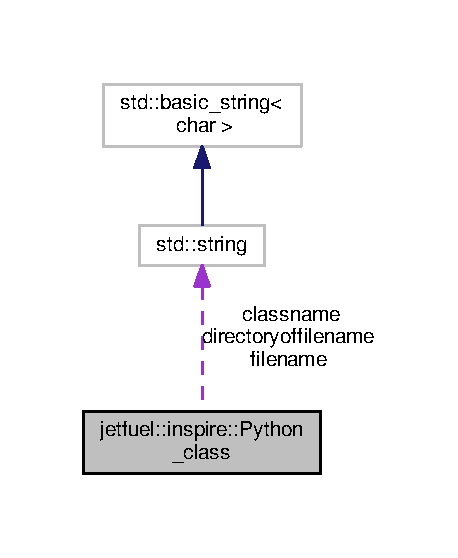
\includegraphics[width=220pt]{structjetfuel_1_1inspire_1_1Python__class__coll__graph}
\end{center}
\end{figure}
\subsection*{Public Attributes}
\begin{DoxyCompactItemize}
\item 
\mbox{\Hypertarget{structjetfuel_1_1inspire_1_1Python__class_ace064af1cb731082b6b28cd0c7fbf354}\label{structjetfuel_1_1inspire_1_1Python__class_ace064af1cb731082b6b28cd0c7fbf354}} 
Py\+Object $\ast$ {\bfseries constructorargs}
\item 
\mbox{\Hypertarget{structjetfuel_1_1inspire_1_1Python__class_ac2ae44bee8c12dc57d0e3b7b816dc14e}\label{structjetfuel_1_1inspire_1_1Python__class_ac2ae44bee8c12dc57d0e3b7b816dc14e}} 
std\+::string {\bfseries filename}
\item 
\mbox{\Hypertarget{structjetfuel_1_1inspire_1_1Python__class_a44270e68f3642d9a268ff4ae726e65f0}\label{structjetfuel_1_1inspire_1_1Python__class_a44270e68f3642d9a268ff4ae726e65f0}} 
std\+::string {\bfseries classname}
\item 
\mbox{\Hypertarget{structjetfuel_1_1inspire_1_1Python__class_a5ce967f2eb9997141355a6eb05113063}\label{structjetfuel_1_1inspire_1_1Python__class_a5ce967f2eb9997141355a6eb05113063}} 
std\+::string {\bfseries directoryoffilename}
\end{DoxyCompactItemize}


\subsection{Detailed Description}
A simple struct representing a Python class.

\begin{DoxySeeAlso}{See also}
\hyperlink{classjetfuel_1_1inspire_1_1Python__class__loader}{jetfuel\+::inspire\+::\+Python\+\_\+class\+\_\+loader} 
\end{DoxySeeAlso}


The documentation for this struct was generated from the following file\+:\begin{DoxyCompactItemize}
\item 
include/jetfuelinspire/pythonclassloader.\+h\end{DoxyCompactItemize}

\hypertarget{classjetfuel_1_1inspire_1_1Python__class__loader}{}\section{jetfuel\+:\+:inspire\+:\+:Python\+\_\+class\+\_\+loader Class Reference}
\label{classjetfuel_1_1inspire_1_1Python__class__loader}\index{jetfuel\+::inspire\+::\+Python\+\_\+class\+\_\+loader@{jetfuel\+::inspire\+::\+Python\+\_\+class\+\_\+loader}}


{\ttfamily \#include $<$pythonclassloader.\+h$>$}

\subsection*{Public Member Functions}
\begin{DoxyCompactItemize}
\item 
\hyperlink{classjetfuel_1_1inspire_1_1Python__class__loader_ae8e3d2e3e2b95a5463f5735f2c0f6be2}{Python\+\_\+class\+\_\+loader} (Py\+Object $\ast$constructorargs, std\+::string $\ast$filename, std\+::string $\ast$classname, bool $\ast$executed, std\+::string $\ast$error, std\+::string $\ast$directoryoffilename)
\begin{DoxyCompactList}\small\item\em Constructs a simple Python class by constructing a Python object given to this function(without using the \hyperlink{structjetfuel_1_1inspire_1_1Python__class}{Python\+\_\+class} struct. \end{DoxyCompactList}\item 
\hyperlink{classjetfuel_1_1inspire_1_1Python__class__loader_a5c52b32bf4e0d5692a20dc652d872da8}{Python\+\_\+class\+\_\+loader} (\hyperlink{structjetfuel_1_1inspire_1_1Python__class}{Python\+\_\+class} \hyperlink{classjetfuel_1_1inspire_1_1Python__class__loader_adbcf46681199db320a6b09aec18a2ca8}{pythonclass}, bool $\ast$executed, std\+::string $\ast$error)
\begin{DoxyCompactList}\small\item\em Constructs a simple Python class by constructing a Python object given to this function(using the \hyperlink{structjetfuel_1_1inspire_1_1Python__class}{Python\+\_\+class} struct). \end{DoxyCompactList}\item 
virtual \hyperlink{classjetfuel_1_1inspire_1_1Python__class__loader_af211621190c98b14234cd23f7f34aeb9}{$\sim$\+Python\+\_\+class\+\_\+loader} ()
\begin{DoxyCompactList}\small\item\em Virtual Destructor. \end{DoxyCompactList}\end{DoxyCompactItemize}
\subsection*{Public Attributes}
\begin{DoxyCompactItemize}
\item 
Py\+Object $\ast$ \hyperlink{classjetfuel_1_1inspire_1_1Python__class__loader_adbcf46681199db320a6b09aec18a2ca8}{pythonclass}
\end{DoxyCompactItemize}


\subsection{Detailed Description}
A Python class loader that allows you to mainuplate Python class from C++.

Code Example\+:

Python(classexample.\+py)\+:

class classexample\+: def {\bfseries init}(self) \+: print(\char`\"{}classexample inited!\char`\"{}); def sayhello(self, name) \+: print(\char`\"{}\+Hello\char`\"{} + name);

C++\+: bool executedstatus; std\+::string fileandclassname = \char`\"{}classexample\char`\"{}; std\+::string directory = \char`\"{}./\+Scripts\char`\"{};

\begin{DoxyVerb}jetfuel::inspire::Python_class_loader classloader(nullptr, 
                        &fileandclassname,&fileandclassname,
                        &executedstatus, &error, &directory);

if(!executedstatus){
    std::cout << "Python Interpreter ERROR! Error is:" << error
    << std::endl;
}

jetfuel::inspire::Python_module_loader classfunction(
                        &classloader,std::string("sayhello"));
executedstatus = bool();

bool returnvalue = classfunctiontester.Execute_bool(
                                    &executedstatus, &error, 
                PyTuple_Pack(1, PyUnicode_FromString("G'day")));
if (!executedstatus) {
    std::cout << "Python Interpreter ERROR! Error is:" << 
    error << std::endl;
}  \end{DoxyVerb}
 

\subsection{Constructor \& Destructor Documentation}
\mbox{\Hypertarget{classjetfuel_1_1inspire_1_1Python__class__loader_ae8e3d2e3e2b95a5463f5735f2c0f6be2}\label{classjetfuel_1_1inspire_1_1Python__class__loader_ae8e3d2e3e2b95a5463f5735f2c0f6be2}} 
\index{jetfuel\+::inspire\+::\+Python\+\_\+class\+\_\+loader@{jetfuel\+::inspire\+::\+Python\+\_\+class\+\_\+loader}!Python\+\_\+class\+\_\+loader@{Python\+\_\+class\+\_\+loader}}
\index{Python\+\_\+class\+\_\+loader@{Python\+\_\+class\+\_\+loader}!jetfuel\+::inspire\+::\+Python\+\_\+class\+\_\+loader@{jetfuel\+::inspire\+::\+Python\+\_\+class\+\_\+loader}}
\subsubsection{\texorpdfstring{Python\+\_\+class\+\_\+loader()}{Python\_class\_loader()}\hspace{0.1cm}{\footnotesize\ttfamily [1/2]}}
{\footnotesize\ttfamily jetfuel\+::inspire\+::\+Python\+\_\+class\+\_\+loader\+::\+Python\+\_\+class\+\_\+loader (\begin{DoxyParamCaption}\item[{Py\+Object $\ast$}]{constructorargs,  }\item[{std\+::string $\ast$}]{filename,  }\item[{std\+::string $\ast$}]{classname,  }\item[{bool $\ast$}]{executed,  }\item[{std\+::string $\ast$}]{error,  }\item[{std\+::string $\ast$}]{directoryoffilename }\end{DoxyParamCaption})}



Constructs a simple Python class by constructing a Python object given to this function(without using the \hyperlink{structjetfuel_1_1inspire_1_1Python__class}{Python\+\_\+class} struct. 

Constructs a simple Python class by constructing a Python object given to this function(without using the \hyperlink{structjetfuel_1_1inspire_1_1Python__class}{Python\+\_\+class} struct).


\begin{DoxyParams}{Parameters}
{\em Py\+Object} & $\ast$constructorargs \\
\hline
{\em std\+::string} & $\ast$filename \\
\hline
{\em std\+::string} & $\ast$classname \\
\hline
{\em bool} & $\ast$executed \\
\hline
{\em std\+::string} & $\ast$error \\
\hline
{\em std\+::string} & $\ast$directoryoffilename \\
\hline
\end{DoxyParams}
\mbox{\Hypertarget{classjetfuel_1_1inspire_1_1Python__class__loader_a5c52b32bf4e0d5692a20dc652d872da8}\label{classjetfuel_1_1inspire_1_1Python__class__loader_a5c52b32bf4e0d5692a20dc652d872da8}} 
\index{jetfuel\+::inspire\+::\+Python\+\_\+class\+\_\+loader@{jetfuel\+::inspire\+::\+Python\+\_\+class\+\_\+loader}!Python\+\_\+class\+\_\+loader@{Python\+\_\+class\+\_\+loader}}
\index{Python\+\_\+class\+\_\+loader@{Python\+\_\+class\+\_\+loader}!jetfuel\+::inspire\+::\+Python\+\_\+class\+\_\+loader@{jetfuel\+::inspire\+::\+Python\+\_\+class\+\_\+loader}}
\subsubsection{\texorpdfstring{Python\+\_\+class\+\_\+loader()}{Python\_class\_loader()}\hspace{0.1cm}{\footnotesize\ttfamily [2/2]}}
{\footnotesize\ttfamily jetfuel\+::inspire\+::\+Python\+\_\+class\+\_\+loader\+::\+Python\+\_\+class\+\_\+loader (\begin{DoxyParamCaption}\item[{\hyperlink{structjetfuel_1_1inspire_1_1Python__class}{Python\+\_\+class}}]{pythonclass,  }\item[{bool $\ast$}]{executed,  }\item[{std\+::string $\ast$}]{error }\end{DoxyParamCaption})}



Constructs a simple Python class by constructing a Python object given to this function(using the \hyperlink{structjetfuel_1_1inspire_1_1Python__class}{Python\+\_\+class} struct). 

Constructs a simple Python class by constructing a Python object given to this function(using \hyperlink{structjetfuel_1_1inspire_1_1Python__class}{Python\+\_\+class} struct).


\begin{DoxyParams}{Parameters}
{\em \hyperlink{structjetfuel_1_1inspire_1_1Python__class}{Python\+\_\+class}} & pythonclass \\
\hline
{\em bool} & $\ast$executed \\
\hline
{\em std\+::string} & $\ast$error \\
\hline
\end{DoxyParams}
\mbox{\Hypertarget{classjetfuel_1_1inspire_1_1Python__class__loader_af211621190c98b14234cd23f7f34aeb9}\label{classjetfuel_1_1inspire_1_1Python__class__loader_af211621190c98b14234cd23f7f34aeb9}} 
\index{jetfuel\+::inspire\+::\+Python\+\_\+class\+\_\+loader@{jetfuel\+::inspire\+::\+Python\+\_\+class\+\_\+loader}!````~Python\+\_\+class\+\_\+loader@{$\sim$\+Python\+\_\+class\+\_\+loader}}
\index{````~Python\+\_\+class\+\_\+loader@{$\sim$\+Python\+\_\+class\+\_\+loader}!jetfuel\+::inspire\+::\+Python\+\_\+class\+\_\+loader@{jetfuel\+::inspire\+::\+Python\+\_\+class\+\_\+loader}}
\subsubsection{\texorpdfstring{$\sim$\+Python\+\_\+class\+\_\+loader()}{~Python\_class\_loader()}}
{\footnotesize\ttfamily virtual jetfuel\+::inspire\+::\+Python\+\_\+class\+\_\+loader\+::$\sim$\+Python\+\_\+class\+\_\+loader (\begin{DoxyParamCaption}{ }\end{DoxyParamCaption})\hspace{0.3cm}{\ttfamily [virtual]}}



Virtual Destructor. 

Destroys this \hyperlink{classjetfuel_1_1inspire_1_1Python__class__loader}{Python\+\_\+class\+\_\+loader} object. 

\subsection{Member Data Documentation}
\mbox{\Hypertarget{classjetfuel_1_1inspire_1_1Python__class__loader_adbcf46681199db320a6b09aec18a2ca8}\label{classjetfuel_1_1inspire_1_1Python__class__loader_adbcf46681199db320a6b09aec18a2ca8}} 
\index{jetfuel\+::inspire\+::\+Python\+\_\+class\+\_\+loader@{jetfuel\+::inspire\+::\+Python\+\_\+class\+\_\+loader}!pythonclass@{pythonclass}}
\index{pythonclass@{pythonclass}!jetfuel\+::inspire\+::\+Python\+\_\+class\+\_\+loader@{jetfuel\+::inspire\+::\+Python\+\_\+class\+\_\+loader}}
\subsubsection{\texorpdfstring{pythonclass}{pythonclass}}
{\footnotesize\ttfamily Py\+Object$\ast$ jetfuel\+::inspire\+::\+Python\+\_\+class\+\_\+loader\+::pythonclass}

The object representing the Python class. 

The documentation for this class was generated from the following file\+:\begin{DoxyCompactItemize}
\item 
include/jetfuelinspire/pythonclassloader.\+h\end{DoxyCompactItemize}

\hypertarget{classjetfuel_1_1inspire_1_1Python__module__loader}{}\section{jetfuel\+:\+:inspire\+:\+:Python\+\_\+module\+\_\+loader Class Reference}
\label{classjetfuel_1_1inspire_1_1Python__module__loader}\index{jetfuel\+::inspire\+::\+Python\+\_\+module\+\_\+loader@{jetfuel\+::inspire\+::\+Python\+\_\+module\+\_\+loader}}
\subsection*{Public Member Functions}
\begin{DoxyCompactItemize}
\item 
\hyperlink{classjetfuel_1_1inspire_1_1Python__module__loader_a30ab85906d5365ca34ca47b456460353}{Python\+\_\+module\+\_\+loader} (const std\+::string filename, const std\+::string functionname, const std\+::string directoryoffilename=\char`\"{}.\char`\"{}, const std\+::string filetoreplace=\char`\"{}\char`\"{}, const std\+::string directoryoffiletoreplace=\char`\"{}.\char`\"{})
\begin{DoxyCompactList}\small\item\em Constructs a \hyperlink{classjetfuel_1_1inspire_1_1Python__module__loader}{Python\+\_\+module\+\_\+loader} using a file-\/name, a functionname, the directory, and, optionally a file to replace the former. \end{DoxyCompactList}\item 
\hyperlink{classjetfuel_1_1inspire_1_1Python__module__loader_addb900473108ecea10d36eceb9917920}{Python\+\_\+module\+\_\+loader} (\hyperlink{classjetfuel_1_1inspire_1_1Python__class__loader}{jetfuel\+::inspire\+::\+Python\+\_\+class\+\_\+loader} $\ast$pythonclasstouse, const std\+::string functionname)
\begin{DoxyCompactList}\small\item\em Constructs a \hyperlink{classjetfuel_1_1inspire_1_1Python__module__loader}{Python\+\_\+module\+\_\+loader} that will load a function from a class. \end{DoxyCompactList}\item 
virtual \hyperlink{classjetfuel_1_1inspire_1_1Python__module__loader_a87c6c13c50ca78e59e19d291355a8bc5}{$\sim$\+Python\+\_\+module\+\_\+loader} ()
\begin{DoxyCompactList}\small\item\em Virtual destructor. \end{DoxyCompactList}\item 
void \hyperlink{classjetfuel_1_1inspire_1_1Python__module__loader_a99f8d8ee9f65c15b10b91ba7e59033c0}{Execute} (bool $\ast$executed, std\+::string $\ast$error, Py\+Object $\ast$args)
\begin{DoxyCompactList}\small\item\em Executes this Python module without any return type. \end{DoxyCompactList}\item 
bool \hyperlink{classjetfuel_1_1inspire_1_1Python__module__loader_a3c51521e298f05b5fbb702327aa102b3}{Execute\+\_\+bool} (bool $\ast$executed, std\+::string $\ast$error, Py\+Object $\ast$args)
\begin{DoxyCompactList}\small\item\em Executes this Python module with a boolean return type. \end{DoxyCompactList}\item 
long \hyperlink{classjetfuel_1_1inspire_1_1Python__module__loader_a7f1608c46e4d3c9f7a019f80a78c6756}{Execute\+\_\+long} (bool $\ast$executed, std\+::string $\ast$error, Py\+Object $\ast$args)
\begin{DoxyCompactList}\small\item\em Executes this Python module with a long return type. \end{DoxyCompactList}\item 
double \hyperlink{classjetfuel_1_1inspire_1_1Python__module__loader_a058df0a03f3477bb7d576d5873246aa7}{Execute\+\_\+double} (bool $\ast$executed, std\+::string $\ast$error, Py\+Object $\ast$args)
\begin{DoxyCompactList}\small\item\em Executes this Python module with a double return type. \end{DoxyCompactList}\item 
char $\ast$ \hyperlink{classjetfuel_1_1inspire_1_1Python__module__loader_a83af544f1b515c3606ed91e9c8ba9494}{Execute\+\_\+cstring} (bool $\ast$executed, std\+::string $\ast$error, Py\+Object $\ast$args)
\begin{DoxyCompactList}\small\item\em Executes this Python module with a cstring return type. \end{DoxyCompactList}\end{DoxyCompactItemize}
\subsection*{Static Public Member Functions}
\begin{DoxyCompactItemize}
\item 
static std\+::string \hyperlink{classjetfuel_1_1inspire_1_1Python__module__loader_a50d20a6fcd26caf7aa1ece5c479bbc01}{Py\+\_\+err\+\_\+to\+\_\+string} (Py\+Object $\ast$pythonerrortype, Py\+Object $\ast$pythonerrorvalue, Py\+Object $\ast$pythonerrortraceback)
\begin{DoxyCompactList}\small\item\em Converts a Python error message to a std\+::string. \end{DoxyCompactList}\item 
static void \hyperlink{classjetfuel_1_1inspire_1_1Python__module__loader_ad8cf860545d85af78f7cc82d4e889840}{Add\+\_\+to\+\_\+py\+\_\+path} (const std\+::string pathlocationtoadd)
\begin{DoxyCompactList}\small\item\em Adds a given directory path to the python path. \end{DoxyCompactList}\end{DoxyCompactItemize}
\subsection*{Protected Member Functions}
\begin{DoxyCompactItemize}
\item 
void \hyperlink{classjetfuel_1_1inspire_1_1Python__module__loader_a54677f790da88ca5ff397555449efafc}{Base\+\_\+execute\+\_\+py\+\_\+object} (Py\+Object $\ast$pythonfunction, Py\+Object $\ast$args, bool $\ast$executed, std\+::string $\ast$error)
\begin{DoxyCompactList}\small\item\em Sets up Python function objects for execution. \end{DoxyCompactList}\item 
void \hyperlink{classjetfuel_1_1inspire_1_1Python__module__loader_a0df6c4f0f9b7fb8fcd97483e6eb841a8}{Execute\+\_\+py\+\_\+object} (Py\+Object $\ast$args, bool $\ast$executed, std\+::string $\ast$error)
\begin{DoxyCompactList}\small\item\em Executes a python function without a return type. \end{DoxyCompactList}\item 
bool \hyperlink{classjetfuel_1_1inspire_1_1Python__module__loader_a97bac700d3f89eb294f438802c82667f}{Execute\+\_\+py\+\_\+object\+\_\+bool} (Py\+Object $\ast$args, bool $\ast$executed, std\+::string $\ast$error)
\begin{DoxyCompactList}\small\item\em Executes a python function with a boolean return type. \end{DoxyCompactList}\item 
long \hyperlink{classjetfuel_1_1inspire_1_1Python__module__loader_a05e19263c55ee6d5acc5e22b00e03e55}{Execute\+\_\+py\+\_\+object\+\_\+long} (Py\+Object $\ast$args, bool $\ast$executed, std\+::string $\ast$error)
\begin{DoxyCompactList}\small\item\em Executes a python function with a long return type. \end{DoxyCompactList}\item 
double \hyperlink{classjetfuel_1_1inspire_1_1Python__module__loader_a0fca60192c29e3f7db689c366fd73437}{Execute\+\_\+py\+\_\+object\+\_\+double} (Py\+Object $\ast$args, bool $\ast$executed, std\+::string $\ast$error)
\begin{DoxyCompactList}\small\item\em Executes a python function with a double return type. \end{DoxyCompactList}\item 
char $\ast$ \hyperlink{classjetfuel_1_1inspire_1_1Python__module__loader_a6dcb9763f793360e89da5f3377a945b9}{Execute\+\_\+py\+\_\+object\+\_\+cstring} (Py\+Object $\ast$args, bool $\ast$executed, std\+::string $\ast$error)
\begin{DoxyCompactList}\small\item\em Executes a python function with a cstring return type. \end{DoxyCompactList}\item 
std\+::string \hyperlink{classjetfuel_1_1inspire_1_1Python__module__loader_a2629d9d235cf65a7fe6f44a2554d317c}{Get\+\_\+file\+\_\+name} () const
\begin{DoxyCompactList}\small\item\em Gets this Python file name. \end{DoxyCompactList}\item 
std\+::string \hyperlink{classjetfuel_1_1inspire_1_1Python__module__loader_af687d8cd4118ea0d4449d00161f00043}{Get\+\_\+file\+\_\+to\+\_\+replace} () const
\begin{DoxyCompactList}\small\item\em Gets this Python file name of the file to replace. \end{DoxyCompactList}\item 
std\+::string \hyperlink{classjetfuel_1_1inspire_1_1Python__module__loader_ad2034cdd073b263cecca65e5bb286745}{Get\+\_\+function\+\_\+name} () const
\begin{DoxyCompactList}\small\item\em Gets this Python function name. \end{DoxyCompactList}\item 
std\+::string \hyperlink{classjetfuel_1_1inspire_1_1Python__module__loader_a11defce7f1f1ae5926744d8e0f01243c}{Get\+\_\+directory\+\_\+of\+\_\+file\+\_\+name} () const
\begin{DoxyCompactList}\small\item\em Gets this directory name of the Python files. \end{DoxyCompactList}\item 
std\+::string \hyperlink{classjetfuel_1_1inspire_1_1Python__module__loader_ae908aab386db9d4d5c20c350d1743b5e}{Get\+\_\+directory\+\_\+of\+\_\+file\+\_\+to\+\_\+replace} () const
\begin{DoxyCompactList}\small\item\em Gets this directory name of the Python files to replace. \end{DoxyCompactList}\item 
bool \hyperlink{classjetfuel_1_1inspire_1_1Python__module__loader_a48f19613015ba3e143827a9946e436cd}{Using\+\_\+classes} () const
\begin{DoxyCompactList}\small\item\em Returns a boolean whether this \hyperlink{classjetfuel_1_1inspire_1_1Python__module__loader}{Python\+\_\+module\+\_\+loader} is invoking class methods. \end{DoxyCompactList}\end{DoxyCompactItemize}
\subsection*{Static Protected Member Functions}
\begin{DoxyCompactItemize}
\item 
static wchar\+\_\+t $\ast$ \hyperlink{classjetfuel_1_1inspire_1_1Python__module__loader_ad4fb50f7f68749decfeef1204fe06acb}{Get\+\_\+wchar} (const char $\ast$chartouse)
\begin{DoxyCompactList}\small\item\em Converts a const char $\ast$ to a wchar\+\_\+t $\ast$. \end{DoxyCompactList}\item 
static const std\+::string \hyperlink{classjetfuel_1_1inspire_1_1Python__module__loader_a88da3316adbe919080ad1c92045b4ad3}{Get\+\_\+string} (const wchar\+\_\+t $\ast$widechar)
\begin{DoxyCompactList}\small\item\em Converts an A\+S\+C\+II wchar\+\_\+t $\ast$ to an A\+S\+C\+II std\+::string. \end{DoxyCompactList}\item 
\mbox{\Hypertarget{classjetfuel_1_1inspire_1_1Python__module__loader_adb872547c2aec3b27e5845fedb7a3f42}\label{classjetfuel_1_1inspire_1_1Python__module__loader_adb872547c2aec3b27e5845fedb7a3f42}} 
static std\+::string {\bfseries Get\+\_\+py\+\_\+error} (Py\+Object $\ast$errorobject)
\end{DoxyCompactItemize}
\subsection*{Protected Attributes}
\begin{DoxyCompactItemize}
\item 
Py\+Object $\ast$ \hyperlink{classjetfuel_1_1inspire_1_1Python__module__loader_a973a8f86d446820b38b18f87fe51465a}{pythonclass}
\end{DoxyCompactItemize}


\subsection{Constructor \& Destructor Documentation}
\mbox{\Hypertarget{classjetfuel_1_1inspire_1_1Python__module__loader_a30ab85906d5365ca34ca47b456460353}\label{classjetfuel_1_1inspire_1_1Python__module__loader_a30ab85906d5365ca34ca47b456460353}} 
\index{jetfuel\+::inspire\+::\+Python\+\_\+module\+\_\+loader@{jetfuel\+::inspire\+::\+Python\+\_\+module\+\_\+loader}!Python\+\_\+module\+\_\+loader@{Python\+\_\+module\+\_\+loader}}
\index{Python\+\_\+module\+\_\+loader@{Python\+\_\+module\+\_\+loader}!jetfuel\+::inspire\+::\+Python\+\_\+module\+\_\+loader@{jetfuel\+::inspire\+::\+Python\+\_\+module\+\_\+loader}}
\subsubsection{\texorpdfstring{Python\+\_\+module\+\_\+loader()}{Python\_module\_loader()}\hspace{0.1cm}{\footnotesize\ttfamily [1/2]}}
{\footnotesize\ttfamily jetfuel\+::inspire\+::\+Python\+\_\+module\+\_\+loader\+::\+Python\+\_\+module\+\_\+loader (\begin{DoxyParamCaption}\item[{const std\+::string}]{filename,  }\item[{const std\+::string}]{functionname,  }\item[{const std\+::string}]{directoryoffilename = {\ttfamily \char`\"{}.\char`\"{}},  }\item[{const std\+::string}]{filetoreplace = {\ttfamily \char`\"{}\char`\"{}},  }\item[{const std\+::string}]{directoryoffiletoreplace = {\ttfamily \char`\"{}.\char`\"{}} }\end{DoxyParamCaption})}



Constructs a \hyperlink{classjetfuel_1_1inspire_1_1Python__module__loader}{Python\+\_\+module\+\_\+loader} using a file-\/name, a functionname, the directory, and, optionally a file to replace the former. 

Constructs a \hyperlink{classjetfuel_1_1inspire_1_1Python__module__loader}{Python\+\_\+module\+\_\+loader} using a file-\/name, a functionname, the directory(set to \char`\"{}.\char`\"{} by default), and, optionally a file to replace the former. If you chose to use the file to replace functionality, the default file will be run first, and then the file to replace will be run second, overriding the first file return value and any Python variables or assignments.

This is handy as a failsafe for a mod system, because if the mod file fails, the game can continue normally, using the internal one function as a failsafe.


\begin{DoxyParams}{Parameters}
{\em std\+::string} & filename \\
\hline
{\em std\+::string} & functionname \\
\hline
{\em std\+::string} & directoryoffilename \\
\hline
{\em std\+::string} & filetoreplace \\
\hline
{\em std\+::string} & directoryoffiletoreplace \\
\hline
\end{DoxyParams}
\mbox{\Hypertarget{classjetfuel_1_1inspire_1_1Python__module__loader_addb900473108ecea10d36eceb9917920}\label{classjetfuel_1_1inspire_1_1Python__module__loader_addb900473108ecea10d36eceb9917920}} 
\index{jetfuel\+::inspire\+::\+Python\+\_\+module\+\_\+loader@{jetfuel\+::inspire\+::\+Python\+\_\+module\+\_\+loader}!Python\+\_\+module\+\_\+loader@{Python\+\_\+module\+\_\+loader}}
\index{Python\+\_\+module\+\_\+loader@{Python\+\_\+module\+\_\+loader}!jetfuel\+::inspire\+::\+Python\+\_\+module\+\_\+loader@{jetfuel\+::inspire\+::\+Python\+\_\+module\+\_\+loader}}
\subsubsection{\texorpdfstring{Python\+\_\+module\+\_\+loader()}{Python\_module\_loader()}\hspace{0.1cm}{\footnotesize\ttfamily [2/2]}}
{\footnotesize\ttfamily jetfuel\+::inspire\+::\+Python\+\_\+module\+\_\+loader\+::\+Python\+\_\+module\+\_\+loader (\begin{DoxyParamCaption}\item[{\hyperlink{classjetfuel_1_1inspire_1_1Python__class__loader}{jetfuel\+::inspire\+::\+Python\+\_\+class\+\_\+loader} $\ast$}]{pythonclasstouse,  }\item[{const std\+::string}]{functionname }\end{DoxyParamCaption})}



Constructs a \hyperlink{classjetfuel_1_1inspire_1_1Python__module__loader}{Python\+\_\+module\+\_\+loader} that will load a function from a class. 

Constructs a \hyperlink{classjetfuel_1_1inspire_1_1Python__module__loader}{Python\+\_\+module\+\_\+loader} that will load a function from a class. This acts like any other \hyperlink{classjetfuel_1_1inspire_1_1Python__module__loader}{Python\+\_\+module\+\_\+loader}, despite the function being from a class.


\begin{DoxyParams}{Parameters}
{\em \hyperlink{classjetfuel_1_1inspire_1_1Python__class__loader}{jetfuel\+::inspire\+::\+Python\+\_\+class\+\_\+loader}} & $\ast$pythonclasstouse \\
\hline
{\em std\+::string} & functionname \\
\hline
\end{DoxyParams}
\mbox{\Hypertarget{classjetfuel_1_1inspire_1_1Python__module__loader_a87c6c13c50ca78e59e19d291355a8bc5}\label{classjetfuel_1_1inspire_1_1Python__module__loader_a87c6c13c50ca78e59e19d291355a8bc5}} 
\index{jetfuel\+::inspire\+::\+Python\+\_\+module\+\_\+loader@{jetfuel\+::inspire\+::\+Python\+\_\+module\+\_\+loader}!````~Python\+\_\+module\+\_\+loader@{$\sim$\+Python\+\_\+module\+\_\+loader}}
\index{````~Python\+\_\+module\+\_\+loader@{$\sim$\+Python\+\_\+module\+\_\+loader}!jetfuel\+::inspire\+::\+Python\+\_\+module\+\_\+loader@{jetfuel\+::inspire\+::\+Python\+\_\+module\+\_\+loader}}
\subsubsection{\texorpdfstring{$\sim$\+Python\+\_\+module\+\_\+loader()}{~Python\_module\_loader()}}
{\footnotesize\ttfamily virtual jetfuel\+::inspire\+::\+Python\+\_\+module\+\_\+loader\+::$\sim$\+Python\+\_\+module\+\_\+loader (\begin{DoxyParamCaption}{ }\end{DoxyParamCaption})\hspace{0.3cm}{\ttfamily [virtual]}}



Virtual destructor. 

Destroys this \hyperlink{classjetfuel_1_1inspire_1_1Python__module__loader}{Python\+\_\+module\+\_\+loader}. 

\subsection{Member Function Documentation}
\mbox{\Hypertarget{classjetfuel_1_1inspire_1_1Python__module__loader_ad8cf860545d85af78f7cc82d4e889840}\label{classjetfuel_1_1inspire_1_1Python__module__loader_ad8cf860545d85af78f7cc82d4e889840}} 
\index{jetfuel\+::inspire\+::\+Python\+\_\+module\+\_\+loader@{jetfuel\+::inspire\+::\+Python\+\_\+module\+\_\+loader}!Add\+\_\+to\+\_\+py\+\_\+path@{Add\+\_\+to\+\_\+py\+\_\+path}}
\index{Add\+\_\+to\+\_\+py\+\_\+path@{Add\+\_\+to\+\_\+py\+\_\+path}!jetfuel\+::inspire\+::\+Python\+\_\+module\+\_\+loader@{jetfuel\+::inspire\+::\+Python\+\_\+module\+\_\+loader}}
\subsubsection{\texorpdfstring{Add\+\_\+to\+\_\+py\+\_\+path()}{Add\_to\_py\_path()}}
{\footnotesize\ttfamily static void jetfuel\+::inspire\+::\+Python\+\_\+module\+\_\+loader\+::\+Add\+\_\+to\+\_\+py\+\_\+path (\begin{DoxyParamCaption}\item[{const std\+::string}]{pathlocationtoadd }\end{DoxyParamCaption})\hspace{0.3cm}{\ttfamily [static]}}



Adds a given directory path to the python path. 

Adds a given directory path to the python path.


\begin{DoxyParams}{Parameters}
{\em std\+::string} & pathlocationtoadd \\
\hline
\end{DoxyParams}
\mbox{\Hypertarget{classjetfuel_1_1inspire_1_1Python__module__loader_a54677f790da88ca5ff397555449efafc}\label{classjetfuel_1_1inspire_1_1Python__module__loader_a54677f790da88ca5ff397555449efafc}} 
\index{jetfuel\+::inspire\+::\+Python\+\_\+module\+\_\+loader@{jetfuel\+::inspire\+::\+Python\+\_\+module\+\_\+loader}!Base\+\_\+execute\+\_\+py\+\_\+object@{Base\+\_\+execute\+\_\+py\+\_\+object}}
\index{Base\+\_\+execute\+\_\+py\+\_\+object@{Base\+\_\+execute\+\_\+py\+\_\+object}!jetfuel\+::inspire\+::\+Python\+\_\+module\+\_\+loader@{jetfuel\+::inspire\+::\+Python\+\_\+module\+\_\+loader}}
\subsubsection{\texorpdfstring{Base\+\_\+execute\+\_\+py\+\_\+object()}{Base\_execute\_py\_object()}}
{\footnotesize\ttfamily void jetfuel\+::inspire\+::\+Python\+\_\+module\+\_\+loader\+::\+Base\+\_\+execute\+\_\+py\+\_\+object (\begin{DoxyParamCaption}\item[{Py\+Object $\ast$}]{pythonfunction,  }\item[{Py\+Object $\ast$}]{args,  }\item[{bool $\ast$}]{executed,  }\item[{std\+::string $\ast$}]{error }\end{DoxyParamCaption})\hspace{0.3cm}{\ttfamily [protected]}}



Sets up Python function objects for execution. 

Sets up Python function objects for execution.


\begin{DoxyParams}{Parameters}
{\em Py\+Object} & $\ast$pythonfunction \\
\hline
{\em Py\+Object} & $\ast$args \\
\hline
{\em bool} & $\ast$executed \\
\hline
{\em std\+::string} & $\ast$error \\
\hline
\end{DoxyParams}
\mbox{\Hypertarget{classjetfuel_1_1inspire_1_1Python__module__loader_a99f8d8ee9f65c15b10b91ba7e59033c0}\label{classjetfuel_1_1inspire_1_1Python__module__loader_a99f8d8ee9f65c15b10b91ba7e59033c0}} 
\index{jetfuel\+::inspire\+::\+Python\+\_\+module\+\_\+loader@{jetfuel\+::inspire\+::\+Python\+\_\+module\+\_\+loader}!Execute@{Execute}}
\index{Execute@{Execute}!jetfuel\+::inspire\+::\+Python\+\_\+module\+\_\+loader@{jetfuel\+::inspire\+::\+Python\+\_\+module\+\_\+loader}}
\subsubsection{\texorpdfstring{Execute()}{Execute()}}
{\footnotesize\ttfamily void jetfuel\+::inspire\+::\+Python\+\_\+module\+\_\+loader\+::\+Execute (\begin{DoxyParamCaption}\item[{bool $\ast$}]{executed,  }\item[{std\+::string $\ast$}]{error,  }\item[{Py\+Object $\ast$}]{args }\end{DoxyParamCaption})}



Executes this Python module without any return type. 

Executes this Python module without any return type. If there are no Python arguments, you can just pass N\+U\+L\+L/nullptr to the last argument of this function.


\begin{DoxyParams}{Parameters}
{\em bool} & $\ast$executed \\
\hline
{\em std\+::string} & $\ast$error \\
\hline
{\em Py\+Object} & $\ast$args \\
\hline
\end{DoxyParams}
\mbox{\Hypertarget{classjetfuel_1_1inspire_1_1Python__module__loader_a3c51521e298f05b5fbb702327aa102b3}\label{classjetfuel_1_1inspire_1_1Python__module__loader_a3c51521e298f05b5fbb702327aa102b3}} 
\index{jetfuel\+::inspire\+::\+Python\+\_\+module\+\_\+loader@{jetfuel\+::inspire\+::\+Python\+\_\+module\+\_\+loader}!Execute\+\_\+bool@{Execute\+\_\+bool}}
\index{Execute\+\_\+bool@{Execute\+\_\+bool}!jetfuel\+::inspire\+::\+Python\+\_\+module\+\_\+loader@{jetfuel\+::inspire\+::\+Python\+\_\+module\+\_\+loader}}
\subsubsection{\texorpdfstring{Execute\+\_\+bool()}{Execute\_bool()}}
{\footnotesize\ttfamily bool jetfuel\+::inspire\+::\+Python\+\_\+module\+\_\+loader\+::\+Execute\+\_\+bool (\begin{DoxyParamCaption}\item[{bool $\ast$}]{executed,  }\item[{std\+::string $\ast$}]{error,  }\item[{Py\+Object $\ast$}]{args }\end{DoxyParamCaption})}



Executes this Python module with a boolean return type. 

Executes this Python module with a boolean return type. If there are no Python arguments, you can just pass N\+U\+L\+L/nullptr to the last argument of this function.


\begin{DoxyParams}{Parameters}
{\em bool} & $\ast$executed \\
\hline
{\em std\+::string} & $\ast$error \\
\hline
{\em Py\+Object} & $\ast$args \\
\hline
\end{DoxyParams}
\mbox{\Hypertarget{classjetfuel_1_1inspire_1_1Python__module__loader_a83af544f1b515c3606ed91e9c8ba9494}\label{classjetfuel_1_1inspire_1_1Python__module__loader_a83af544f1b515c3606ed91e9c8ba9494}} 
\index{jetfuel\+::inspire\+::\+Python\+\_\+module\+\_\+loader@{jetfuel\+::inspire\+::\+Python\+\_\+module\+\_\+loader}!Execute\+\_\+cstring@{Execute\+\_\+cstring}}
\index{Execute\+\_\+cstring@{Execute\+\_\+cstring}!jetfuel\+::inspire\+::\+Python\+\_\+module\+\_\+loader@{jetfuel\+::inspire\+::\+Python\+\_\+module\+\_\+loader}}
\subsubsection{\texorpdfstring{Execute\+\_\+cstring()}{Execute\_cstring()}}
{\footnotesize\ttfamily char$\ast$ jetfuel\+::inspire\+::\+Python\+\_\+module\+\_\+loader\+::\+Execute\+\_\+cstring (\begin{DoxyParamCaption}\item[{bool $\ast$}]{executed,  }\item[{std\+::string $\ast$}]{error,  }\item[{Py\+Object $\ast$}]{args }\end{DoxyParamCaption})}



Executes this Python module with a cstring return type. 

Executes this Python module with a cstring return type. If there are no Python arguments, you can just pass N\+U\+L\+L/nullptr to the last argument of this function. This serves as the way to also get an std\+::string return type. After you get the long, just convert it to a std\+::string.


\begin{DoxyParams}{Parameters}
{\em bool} & $\ast$executed \\
\hline
{\em std\+::string} & $\ast$error \\
\hline
{\em Py\+Object} & $\ast$args \\
\hline
\end{DoxyParams}
\mbox{\Hypertarget{classjetfuel_1_1inspire_1_1Python__module__loader_a058df0a03f3477bb7d576d5873246aa7}\label{classjetfuel_1_1inspire_1_1Python__module__loader_a058df0a03f3477bb7d576d5873246aa7}} 
\index{jetfuel\+::inspire\+::\+Python\+\_\+module\+\_\+loader@{jetfuel\+::inspire\+::\+Python\+\_\+module\+\_\+loader}!Execute\+\_\+double@{Execute\+\_\+double}}
\index{Execute\+\_\+double@{Execute\+\_\+double}!jetfuel\+::inspire\+::\+Python\+\_\+module\+\_\+loader@{jetfuel\+::inspire\+::\+Python\+\_\+module\+\_\+loader}}
\subsubsection{\texorpdfstring{Execute\+\_\+double()}{Execute\_double()}}
{\footnotesize\ttfamily double jetfuel\+::inspire\+::\+Python\+\_\+module\+\_\+loader\+::\+Execute\+\_\+double (\begin{DoxyParamCaption}\item[{bool $\ast$}]{executed,  }\item[{std\+::string $\ast$}]{error,  }\item[{Py\+Object $\ast$}]{args }\end{DoxyParamCaption})}



Executes this Python module with a double return type. 

Executes this Python module with a double return type. If there are no Python arguments, you can just pass N\+U\+L\+L/nullptr to the last argument of this function. This serves as the way to also get an float return type. After you get the double, just convert it to a float.


\begin{DoxyParams}{Parameters}
{\em bool} & $\ast$executed \\
\hline
{\em std\+::string} & $\ast$error \\
\hline
{\em Py\+Object} & $\ast$args \\
\hline
\end{DoxyParams}
\mbox{\Hypertarget{classjetfuel_1_1inspire_1_1Python__module__loader_a7f1608c46e4d3c9f7a019f80a78c6756}\label{classjetfuel_1_1inspire_1_1Python__module__loader_a7f1608c46e4d3c9f7a019f80a78c6756}} 
\index{jetfuel\+::inspire\+::\+Python\+\_\+module\+\_\+loader@{jetfuel\+::inspire\+::\+Python\+\_\+module\+\_\+loader}!Execute\+\_\+long@{Execute\+\_\+long}}
\index{Execute\+\_\+long@{Execute\+\_\+long}!jetfuel\+::inspire\+::\+Python\+\_\+module\+\_\+loader@{jetfuel\+::inspire\+::\+Python\+\_\+module\+\_\+loader}}
\subsubsection{\texorpdfstring{Execute\+\_\+long()}{Execute\_long()}}
{\footnotesize\ttfamily long jetfuel\+::inspire\+::\+Python\+\_\+module\+\_\+loader\+::\+Execute\+\_\+long (\begin{DoxyParamCaption}\item[{bool $\ast$}]{executed,  }\item[{std\+::string $\ast$}]{error,  }\item[{Py\+Object $\ast$}]{args }\end{DoxyParamCaption})}



Executes this Python module with a long return type. 

Executes this Python module with a long return type. If there are no Python arguments, you can just pass N\+U\+L\+L/nullptr to the last argument of this function. This serves as the way to also get an int return type. After you get the long, just convert it to an int.


\begin{DoxyParams}{Parameters}
{\em bool} & $\ast$executed \\
\hline
{\em std\+::string} & $\ast$error \\
\hline
{\em Py\+Object} & $\ast$args \\
\hline
\end{DoxyParams}
\mbox{\Hypertarget{classjetfuel_1_1inspire_1_1Python__module__loader_a0df6c4f0f9b7fb8fcd97483e6eb841a8}\label{classjetfuel_1_1inspire_1_1Python__module__loader_a0df6c4f0f9b7fb8fcd97483e6eb841a8}} 
\index{jetfuel\+::inspire\+::\+Python\+\_\+module\+\_\+loader@{jetfuel\+::inspire\+::\+Python\+\_\+module\+\_\+loader}!Execute\+\_\+py\+\_\+object@{Execute\+\_\+py\+\_\+object}}
\index{Execute\+\_\+py\+\_\+object@{Execute\+\_\+py\+\_\+object}!jetfuel\+::inspire\+::\+Python\+\_\+module\+\_\+loader@{jetfuel\+::inspire\+::\+Python\+\_\+module\+\_\+loader}}
\subsubsection{\texorpdfstring{Execute\+\_\+py\+\_\+object()}{Execute\_py\_object()}}
{\footnotesize\ttfamily void jetfuel\+::inspire\+::\+Python\+\_\+module\+\_\+loader\+::\+Execute\+\_\+py\+\_\+object (\begin{DoxyParamCaption}\item[{Py\+Object $\ast$}]{args,  }\item[{bool $\ast$}]{executed,  }\item[{std\+::string $\ast$}]{error }\end{DoxyParamCaption})\hspace{0.3cm}{\ttfamily [protected]}}



Executes a python function without a return type. 

Executes a python function without a return type.


\begin{DoxyParams}{Parameters}
{\em Py\+Object} & $\ast$args \\
\hline
{\em bool} & $\ast$executed \\
\hline
{\em std\+::string} & $\ast$error \\
\hline
\end{DoxyParams}
\mbox{\Hypertarget{classjetfuel_1_1inspire_1_1Python__module__loader_a97bac700d3f89eb294f438802c82667f}\label{classjetfuel_1_1inspire_1_1Python__module__loader_a97bac700d3f89eb294f438802c82667f}} 
\index{jetfuel\+::inspire\+::\+Python\+\_\+module\+\_\+loader@{jetfuel\+::inspire\+::\+Python\+\_\+module\+\_\+loader}!Execute\+\_\+py\+\_\+object\+\_\+bool@{Execute\+\_\+py\+\_\+object\+\_\+bool}}
\index{Execute\+\_\+py\+\_\+object\+\_\+bool@{Execute\+\_\+py\+\_\+object\+\_\+bool}!jetfuel\+::inspire\+::\+Python\+\_\+module\+\_\+loader@{jetfuel\+::inspire\+::\+Python\+\_\+module\+\_\+loader}}
\subsubsection{\texorpdfstring{Execute\+\_\+py\+\_\+object\+\_\+bool()}{Execute\_py\_object\_bool()}}
{\footnotesize\ttfamily bool jetfuel\+::inspire\+::\+Python\+\_\+module\+\_\+loader\+::\+Execute\+\_\+py\+\_\+object\+\_\+bool (\begin{DoxyParamCaption}\item[{Py\+Object $\ast$}]{args,  }\item[{bool $\ast$}]{executed,  }\item[{std\+::string $\ast$}]{error }\end{DoxyParamCaption})\hspace{0.3cm}{\ttfamily [protected]}}



Executes a python function with a boolean return type. 

Executes a python function with a boolean return type.


\begin{DoxyParams}{Parameters}
{\em Py\+Object} & $\ast$args \\
\hline
{\em bool} & $\ast$executed \\
\hline
{\em std\+::string} & $\ast$error \\
\hline
\end{DoxyParams}
\mbox{\Hypertarget{classjetfuel_1_1inspire_1_1Python__module__loader_a6dcb9763f793360e89da5f3377a945b9}\label{classjetfuel_1_1inspire_1_1Python__module__loader_a6dcb9763f793360e89da5f3377a945b9}} 
\index{jetfuel\+::inspire\+::\+Python\+\_\+module\+\_\+loader@{jetfuel\+::inspire\+::\+Python\+\_\+module\+\_\+loader}!Execute\+\_\+py\+\_\+object\+\_\+cstring@{Execute\+\_\+py\+\_\+object\+\_\+cstring}}
\index{Execute\+\_\+py\+\_\+object\+\_\+cstring@{Execute\+\_\+py\+\_\+object\+\_\+cstring}!jetfuel\+::inspire\+::\+Python\+\_\+module\+\_\+loader@{jetfuel\+::inspire\+::\+Python\+\_\+module\+\_\+loader}}
\subsubsection{\texorpdfstring{Execute\+\_\+py\+\_\+object\+\_\+cstring()}{Execute\_py\_object\_cstring()}}
{\footnotesize\ttfamily char$\ast$ jetfuel\+::inspire\+::\+Python\+\_\+module\+\_\+loader\+::\+Execute\+\_\+py\+\_\+object\+\_\+cstring (\begin{DoxyParamCaption}\item[{Py\+Object $\ast$}]{args,  }\item[{bool $\ast$}]{executed,  }\item[{std\+::string $\ast$}]{error }\end{DoxyParamCaption})\hspace{0.3cm}{\ttfamily [protected]}}



Executes a python function with a cstring return type. 

Executes a python function with a cstring return type.


\begin{DoxyParams}{Parameters}
{\em Py\+Object} & $\ast$args \\
\hline
{\em bool} & $\ast$executed \\
\hline
{\em std\+::string} & $\ast$error \\
\hline
\end{DoxyParams}
\mbox{\Hypertarget{classjetfuel_1_1inspire_1_1Python__module__loader_a0fca60192c29e3f7db689c366fd73437}\label{classjetfuel_1_1inspire_1_1Python__module__loader_a0fca60192c29e3f7db689c366fd73437}} 
\index{jetfuel\+::inspire\+::\+Python\+\_\+module\+\_\+loader@{jetfuel\+::inspire\+::\+Python\+\_\+module\+\_\+loader}!Execute\+\_\+py\+\_\+object\+\_\+double@{Execute\+\_\+py\+\_\+object\+\_\+double}}
\index{Execute\+\_\+py\+\_\+object\+\_\+double@{Execute\+\_\+py\+\_\+object\+\_\+double}!jetfuel\+::inspire\+::\+Python\+\_\+module\+\_\+loader@{jetfuel\+::inspire\+::\+Python\+\_\+module\+\_\+loader}}
\subsubsection{\texorpdfstring{Execute\+\_\+py\+\_\+object\+\_\+double()}{Execute\_py\_object\_double()}}
{\footnotesize\ttfamily double jetfuel\+::inspire\+::\+Python\+\_\+module\+\_\+loader\+::\+Execute\+\_\+py\+\_\+object\+\_\+double (\begin{DoxyParamCaption}\item[{Py\+Object $\ast$}]{args,  }\item[{bool $\ast$}]{executed,  }\item[{std\+::string $\ast$}]{error }\end{DoxyParamCaption})\hspace{0.3cm}{\ttfamily [protected]}}



Executes a python function with a double return type. 

Executes a python function with a double return type.


\begin{DoxyParams}{Parameters}
{\em Py\+Object} & $\ast$args \\
\hline
{\em bool} & $\ast$executed \\
\hline
{\em std\+::string} & $\ast$error \\
\hline
\end{DoxyParams}
\mbox{\Hypertarget{classjetfuel_1_1inspire_1_1Python__module__loader_a05e19263c55ee6d5acc5e22b00e03e55}\label{classjetfuel_1_1inspire_1_1Python__module__loader_a05e19263c55ee6d5acc5e22b00e03e55}} 
\index{jetfuel\+::inspire\+::\+Python\+\_\+module\+\_\+loader@{jetfuel\+::inspire\+::\+Python\+\_\+module\+\_\+loader}!Execute\+\_\+py\+\_\+object\+\_\+long@{Execute\+\_\+py\+\_\+object\+\_\+long}}
\index{Execute\+\_\+py\+\_\+object\+\_\+long@{Execute\+\_\+py\+\_\+object\+\_\+long}!jetfuel\+::inspire\+::\+Python\+\_\+module\+\_\+loader@{jetfuel\+::inspire\+::\+Python\+\_\+module\+\_\+loader}}
\subsubsection{\texorpdfstring{Execute\+\_\+py\+\_\+object\+\_\+long()}{Execute\_py\_object\_long()}}
{\footnotesize\ttfamily long jetfuel\+::inspire\+::\+Python\+\_\+module\+\_\+loader\+::\+Execute\+\_\+py\+\_\+object\+\_\+long (\begin{DoxyParamCaption}\item[{Py\+Object $\ast$}]{args,  }\item[{bool $\ast$}]{executed,  }\item[{std\+::string $\ast$}]{error }\end{DoxyParamCaption})\hspace{0.3cm}{\ttfamily [protected]}}



Executes a python function with a long return type. 

Executes a python function with a long return type.


\begin{DoxyParams}{Parameters}
{\em Py\+Object} & $\ast$args \\
\hline
{\em bool} & $\ast$executed \\
\hline
{\em std\+::string} & $\ast$error \\
\hline
\end{DoxyParams}
\mbox{\Hypertarget{classjetfuel_1_1inspire_1_1Python__module__loader_a11defce7f1f1ae5926744d8e0f01243c}\label{classjetfuel_1_1inspire_1_1Python__module__loader_a11defce7f1f1ae5926744d8e0f01243c}} 
\index{jetfuel\+::inspire\+::\+Python\+\_\+module\+\_\+loader@{jetfuel\+::inspire\+::\+Python\+\_\+module\+\_\+loader}!Get\+\_\+directory\+\_\+of\+\_\+file\+\_\+name@{Get\+\_\+directory\+\_\+of\+\_\+file\+\_\+name}}
\index{Get\+\_\+directory\+\_\+of\+\_\+file\+\_\+name@{Get\+\_\+directory\+\_\+of\+\_\+file\+\_\+name}!jetfuel\+::inspire\+::\+Python\+\_\+module\+\_\+loader@{jetfuel\+::inspire\+::\+Python\+\_\+module\+\_\+loader}}
\subsubsection{\texorpdfstring{Get\+\_\+directory\+\_\+of\+\_\+file\+\_\+name()}{Get\_directory\_of\_file\_name()}}
{\footnotesize\ttfamily std\+::string jetfuel\+::inspire\+::\+Python\+\_\+module\+\_\+loader\+::\+Get\+\_\+directory\+\_\+of\+\_\+file\+\_\+name (\begin{DoxyParamCaption}{ }\end{DoxyParamCaption}) const\hspace{0.3cm}{\ttfamily [inline]}, {\ttfamily [protected]}}



Gets this directory name of the Python files. 

Gets this directory name of the Python files. \mbox{\Hypertarget{classjetfuel_1_1inspire_1_1Python__module__loader_ae908aab386db9d4d5c20c350d1743b5e}\label{classjetfuel_1_1inspire_1_1Python__module__loader_ae908aab386db9d4d5c20c350d1743b5e}} 
\index{jetfuel\+::inspire\+::\+Python\+\_\+module\+\_\+loader@{jetfuel\+::inspire\+::\+Python\+\_\+module\+\_\+loader}!Get\+\_\+directory\+\_\+of\+\_\+file\+\_\+to\+\_\+replace@{Get\+\_\+directory\+\_\+of\+\_\+file\+\_\+to\+\_\+replace}}
\index{Get\+\_\+directory\+\_\+of\+\_\+file\+\_\+to\+\_\+replace@{Get\+\_\+directory\+\_\+of\+\_\+file\+\_\+to\+\_\+replace}!jetfuel\+::inspire\+::\+Python\+\_\+module\+\_\+loader@{jetfuel\+::inspire\+::\+Python\+\_\+module\+\_\+loader}}
\subsubsection{\texorpdfstring{Get\+\_\+directory\+\_\+of\+\_\+file\+\_\+to\+\_\+replace()}{Get\_directory\_of\_file\_to\_replace()}}
{\footnotesize\ttfamily std\+::string jetfuel\+::inspire\+::\+Python\+\_\+module\+\_\+loader\+::\+Get\+\_\+directory\+\_\+of\+\_\+file\+\_\+to\+\_\+replace (\begin{DoxyParamCaption}{ }\end{DoxyParamCaption}) const\hspace{0.3cm}{\ttfamily [inline]}, {\ttfamily [protected]}}



Gets this directory name of the Python files to replace. 

Gets this directory name of the Python files to replace. \mbox{\Hypertarget{classjetfuel_1_1inspire_1_1Python__module__loader_a2629d9d235cf65a7fe6f44a2554d317c}\label{classjetfuel_1_1inspire_1_1Python__module__loader_a2629d9d235cf65a7fe6f44a2554d317c}} 
\index{jetfuel\+::inspire\+::\+Python\+\_\+module\+\_\+loader@{jetfuel\+::inspire\+::\+Python\+\_\+module\+\_\+loader}!Get\+\_\+file\+\_\+name@{Get\+\_\+file\+\_\+name}}
\index{Get\+\_\+file\+\_\+name@{Get\+\_\+file\+\_\+name}!jetfuel\+::inspire\+::\+Python\+\_\+module\+\_\+loader@{jetfuel\+::inspire\+::\+Python\+\_\+module\+\_\+loader}}
\subsubsection{\texorpdfstring{Get\+\_\+file\+\_\+name()}{Get\_file\_name()}}
{\footnotesize\ttfamily std\+::string jetfuel\+::inspire\+::\+Python\+\_\+module\+\_\+loader\+::\+Get\+\_\+file\+\_\+name (\begin{DoxyParamCaption}{ }\end{DoxyParamCaption}) const\hspace{0.3cm}{\ttfamily [inline]}, {\ttfamily [protected]}}



Gets this Python file name. 

Gets this Python file name. \mbox{\Hypertarget{classjetfuel_1_1inspire_1_1Python__module__loader_af687d8cd4118ea0d4449d00161f00043}\label{classjetfuel_1_1inspire_1_1Python__module__loader_af687d8cd4118ea0d4449d00161f00043}} 
\index{jetfuel\+::inspire\+::\+Python\+\_\+module\+\_\+loader@{jetfuel\+::inspire\+::\+Python\+\_\+module\+\_\+loader}!Get\+\_\+file\+\_\+to\+\_\+replace@{Get\+\_\+file\+\_\+to\+\_\+replace}}
\index{Get\+\_\+file\+\_\+to\+\_\+replace@{Get\+\_\+file\+\_\+to\+\_\+replace}!jetfuel\+::inspire\+::\+Python\+\_\+module\+\_\+loader@{jetfuel\+::inspire\+::\+Python\+\_\+module\+\_\+loader}}
\subsubsection{\texorpdfstring{Get\+\_\+file\+\_\+to\+\_\+replace()}{Get\_file\_to\_replace()}}
{\footnotesize\ttfamily std\+::string jetfuel\+::inspire\+::\+Python\+\_\+module\+\_\+loader\+::\+Get\+\_\+file\+\_\+to\+\_\+replace (\begin{DoxyParamCaption}{ }\end{DoxyParamCaption}) const\hspace{0.3cm}{\ttfamily [inline]}, {\ttfamily [protected]}}



Gets this Python file name of the file to replace. 

Gets this Python file name of the file to replace. \mbox{\Hypertarget{classjetfuel_1_1inspire_1_1Python__module__loader_ad2034cdd073b263cecca65e5bb286745}\label{classjetfuel_1_1inspire_1_1Python__module__loader_ad2034cdd073b263cecca65e5bb286745}} 
\index{jetfuel\+::inspire\+::\+Python\+\_\+module\+\_\+loader@{jetfuel\+::inspire\+::\+Python\+\_\+module\+\_\+loader}!Get\+\_\+function\+\_\+name@{Get\+\_\+function\+\_\+name}}
\index{Get\+\_\+function\+\_\+name@{Get\+\_\+function\+\_\+name}!jetfuel\+::inspire\+::\+Python\+\_\+module\+\_\+loader@{jetfuel\+::inspire\+::\+Python\+\_\+module\+\_\+loader}}
\subsubsection{\texorpdfstring{Get\+\_\+function\+\_\+name()}{Get\_function\_name()}}
{\footnotesize\ttfamily std\+::string jetfuel\+::inspire\+::\+Python\+\_\+module\+\_\+loader\+::\+Get\+\_\+function\+\_\+name (\begin{DoxyParamCaption}{ }\end{DoxyParamCaption}) const\hspace{0.3cm}{\ttfamily [inline]}, {\ttfamily [protected]}}



Gets this Python function name. 

Gets this Python function name. \mbox{\Hypertarget{classjetfuel_1_1inspire_1_1Python__module__loader_a88da3316adbe919080ad1c92045b4ad3}\label{classjetfuel_1_1inspire_1_1Python__module__loader_a88da3316adbe919080ad1c92045b4ad3}} 
\index{jetfuel\+::inspire\+::\+Python\+\_\+module\+\_\+loader@{jetfuel\+::inspire\+::\+Python\+\_\+module\+\_\+loader}!Get\+\_\+string@{Get\+\_\+string}}
\index{Get\+\_\+string@{Get\+\_\+string}!jetfuel\+::inspire\+::\+Python\+\_\+module\+\_\+loader@{jetfuel\+::inspire\+::\+Python\+\_\+module\+\_\+loader}}
\subsubsection{\texorpdfstring{Get\+\_\+string()}{Get\_string()}}
{\footnotesize\ttfamily static const std\+::string jetfuel\+::inspire\+::\+Python\+\_\+module\+\_\+loader\+::\+Get\+\_\+string (\begin{DoxyParamCaption}\item[{const wchar\+\_\+t $\ast$}]{widechar }\end{DoxyParamCaption})\hspace{0.3cm}{\ttfamily [inline]}, {\ttfamily [static]}, {\ttfamily [protected]}}



Converts an A\+S\+C\+II wchar\+\_\+t $\ast$ to an A\+S\+C\+II std\+::string. 

Converts an A\+S\+C\+II wchar\+\_\+t $\ast$ to an A\+S\+C\+II std\+::string.


\begin{DoxyParams}{Parameters}
{\em wchar\+\_\+t$\ast$} & widechar \\
\hline
\end{DoxyParams}
\mbox{\Hypertarget{classjetfuel_1_1inspire_1_1Python__module__loader_ad4fb50f7f68749decfeef1204fe06acb}\label{classjetfuel_1_1inspire_1_1Python__module__loader_ad4fb50f7f68749decfeef1204fe06acb}} 
\index{jetfuel\+::inspire\+::\+Python\+\_\+module\+\_\+loader@{jetfuel\+::inspire\+::\+Python\+\_\+module\+\_\+loader}!Get\+\_\+wchar@{Get\+\_\+wchar}}
\index{Get\+\_\+wchar@{Get\+\_\+wchar}!jetfuel\+::inspire\+::\+Python\+\_\+module\+\_\+loader@{jetfuel\+::inspire\+::\+Python\+\_\+module\+\_\+loader}}
\subsubsection{\texorpdfstring{Get\+\_\+wchar()}{Get\_wchar()}}
{\footnotesize\ttfamily static wchar\+\_\+t$\ast$ jetfuel\+::inspire\+::\+Python\+\_\+module\+\_\+loader\+::\+Get\+\_\+wchar (\begin{DoxyParamCaption}\item[{const char $\ast$}]{chartouse }\end{DoxyParamCaption})\hspace{0.3cm}{\ttfamily [inline]}, {\ttfamily [static]}, {\ttfamily [protected]}}



Converts a const char $\ast$ to a wchar\+\_\+t $\ast$. 

Converts a const char $\ast$ to a wchar\+\_\+t $\ast$.


\begin{DoxyParams}{Parameters}
{\em const} & char $\ast$chartouse \\
\hline
\end{DoxyParams}
\mbox{\Hypertarget{classjetfuel_1_1inspire_1_1Python__module__loader_a50d20a6fcd26caf7aa1ece5c479bbc01}\label{classjetfuel_1_1inspire_1_1Python__module__loader_a50d20a6fcd26caf7aa1ece5c479bbc01}} 
\index{jetfuel\+::inspire\+::\+Python\+\_\+module\+\_\+loader@{jetfuel\+::inspire\+::\+Python\+\_\+module\+\_\+loader}!Py\+\_\+err\+\_\+to\+\_\+string@{Py\+\_\+err\+\_\+to\+\_\+string}}
\index{Py\+\_\+err\+\_\+to\+\_\+string@{Py\+\_\+err\+\_\+to\+\_\+string}!jetfuel\+::inspire\+::\+Python\+\_\+module\+\_\+loader@{jetfuel\+::inspire\+::\+Python\+\_\+module\+\_\+loader}}
\subsubsection{\texorpdfstring{Py\+\_\+err\+\_\+to\+\_\+string()}{Py\_err\_to\_string()}}
{\footnotesize\ttfamily static std\+::string jetfuel\+::inspire\+::\+Python\+\_\+module\+\_\+loader\+::\+Py\+\_\+err\+\_\+to\+\_\+string (\begin{DoxyParamCaption}\item[{Py\+Object $\ast$}]{pythonerrortype,  }\item[{Py\+Object $\ast$}]{pythonerrorvalue,  }\item[{Py\+Object $\ast$}]{pythonerrortraceback }\end{DoxyParamCaption})\hspace{0.3cm}{\ttfamily [static]}}



Converts a Python error message to a std\+::string. 

Converts a Python error message to a std\+::string.


\begin{DoxyParams}{Parameters}
{\em Py\+Object} & $\ast$pythonerrortype \\
\hline
{\em Py\+Object} & $\ast$pythonerrorvalue \\
\hline
{\em Py\+Object} & $\ast$pythonerrortraceback \\
\hline
\end{DoxyParams}
\mbox{\Hypertarget{classjetfuel_1_1inspire_1_1Python__module__loader_a48f19613015ba3e143827a9946e436cd}\label{classjetfuel_1_1inspire_1_1Python__module__loader_a48f19613015ba3e143827a9946e436cd}} 
\index{jetfuel\+::inspire\+::\+Python\+\_\+module\+\_\+loader@{jetfuel\+::inspire\+::\+Python\+\_\+module\+\_\+loader}!Using\+\_\+classes@{Using\+\_\+classes}}
\index{Using\+\_\+classes@{Using\+\_\+classes}!jetfuel\+::inspire\+::\+Python\+\_\+module\+\_\+loader@{jetfuel\+::inspire\+::\+Python\+\_\+module\+\_\+loader}}
\subsubsection{\texorpdfstring{Using\+\_\+classes()}{Using\_classes()}}
{\footnotesize\ttfamily bool jetfuel\+::inspire\+::\+Python\+\_\+module\+\_\+loader\+::\+Using\+\_\+classes (\begin{DoxyParamCaption}{ }\end{DoxyParamCaption}) const\hspace{0.3cm}{\ttfamily [inline]}, {\ttfamily [protected]}}



Returns a boolean whether this \hyperlink{classjetfuel_1_1inspire_1_1Python__module__loader}{Python\+\_\+module\+\_\+loader} is invoking class methods. 

Returns a boolean whether this \hyperlink{classjetfuel_1_1inspire_1_1Python__module__loader}{Python\+\_\+module\+\_\+loader} is invoking class methods. 

\subsection{Member Data Documentation}
\mbox{\Hypertarget{classjetfuel_1_1inspire_1_1Python__module__loader_a973a8f86d446820b38b18f87fe51465a}\label{classjetfuel_1_1inspire_1_1Python__module__loader_a973a8f86d446820b38b18f87fe51465a}} 
\index{jetfuel\+::inspire\+::\+Python\+\_\+module\+\_\+loader@{jetfuel\+::inspire\+::\+Python\+\_\+module\+\_\+loader}!pythonclass@{pythonclass}}
\index{pythonclass@{pythonclass}!jetfuel\+::inspire\+::\+Python\+\_\+module\+\_\+loader@{jetfuel\+::inspire\+::\+Python\+\_\+module\+\_\+loader}}
\subsubsection{\texorpdfstring{pythonclass}{pythonclass}}
{\footnotesize\ttfamily Py\+Object$\ast$ jetfuel\+::inspire\+::\+Python\+\_\+module\+\_\+loader\+::pythonclass\hspace{0.3cm}{\ttfamily [protected]}}

A Python class object used to call Python class methods. 

The documentation for this class was generated from the following file\+:\begin{DoxyCompactItemize}
\item 
include/jetfuelinspire/pythonmoduleloader.\+h\end{DoxyCompactItemize}

\hypertarget{classjetfuel_1_1inspire_1_1exceptions_1_1Python__returnvalue__ASCII__encoding__exception}{}\section{jetfuel\+:\+:inspire\+:\+:exceptions\+:\+:Python\+\_\+returnvalue\+\_\+\+A\+S\+C\+I\+I\+\_\+encoding\+\_\+exception Class Reference}
\label{classjetfuel_1_1inspire_1_1exceptions_1_1Python__returnvalue__ASCII__encoding__exception}\index{jetfuel\+::inspire\+::exceptions\+::\+Python\+\_\+returnvalue\+\_\+\+A\+S\+C\+I\+I\+\_\+encoding\+\_\+exception@{jetfuel\+::inspire\+::exceptions\+::\+Python\+\_\+returnvalue\+\_\+\+A\+S\+C\+I\+I\+\_\+encoding\+\_\+exception}}


Inheritance diagram for jetfuel\+:\+:inspire\+:\+:exceptions\+:\+:Python\+\_\+returnvalue\+\_\+\+A\+S\+C\+I\+I\+\_\+encoding\+\_\+exception\+:
\nopagebreak
\begin{figure}[H]
\begin{center}
\leavevmode
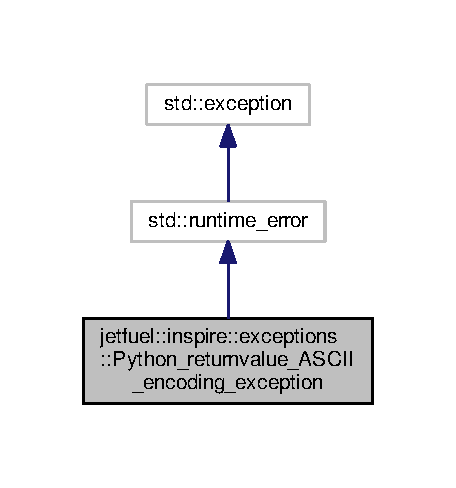
\includegraphics[width=219pt]{classjetfuel_1_1inspire_1_1exceptions_1_1Python__returnvalue__ASCII__encoding__exception__inherit__graph}
\end{center}
\end{figure}


Collaboration diagram for jetfuel\+:\+:inspire\+:\+:exceptions\+:\+:Python\+\_\+returnvalue\+\_\+\+A\+S\+C\+I\+I\+\_\+encoding\+\_\+exception\+:
\nopagebreak
\begin{figure}[H]
\begin{center}
\leavevmode
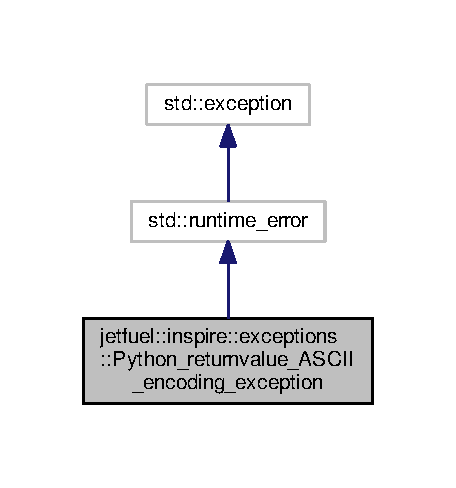
\includegraphics[width=219pt]{classjetfuel_1_1inspire_1_1exceptions_1_1Python__returnvalue__ASCII__encoding__exception__coll__graph}
\end{center}
\end{figure}
\subsection*{Public Member Functions}
\begin{DoxyCompactItemize}
\item 
\mbox{\Hypertarget{classjetfuel_1_1inspire_1_1exceptions_1_1Python__returnvalue__ASCII__encoding__exception_a654d896ec64d3fbb9720e295d52a7f76}\label{classjetfuel_1_1inspire_1_1exceptions_1_1Python__returnvalue__ASCII__encoding__exception_a654d896ec64d3fbb9720e295d52a7f76}} 
{\bfseries Python\+\_\+returnvalue\+\_\+\+A\+S\+C\+I\+I\+\_\+encoding\+\_\+exception} (const std\+::string filename, const std\+::string functionname)
\end{DoxyCompactItemize}


The documentation for this class was generated from the following file\+:\begin{DoxyCompactItemize}
\item 
include/jetfuelinspire/pythonmoduleloader.\+h\end{DoxyCompactItemize}

\hypertarget{classjetfuel_1_1inspire_1_1exceptions_1_1Python__returnvalue__ASCII__encoding__exception}{}\section{jetfuel\+:\+:inspire\+:\+:exceptions\+:\+:Python\+\_\+returnvalue\+\_\+\+A\+S\+C\+I\+I\+\_\+encoding\+\_\+exception Class Reference}
\label{classjetfuel_1_1inspire_1_1exceptions_1_1Python__returnvalue__ASCII__encoding__exception}\index{jetfuel\+::inspire\+::exceptions\+::\+Python\+\_\+returnvalue\+\_\+\+A\+S\+C\+I\+I\+\_\+encoding\+\_\+exception@{jetfuel\+::inspire\+::exceptions\+::\+Python\+\_\+returnvalue\+\_\+\+A\+S\+C\+I\+I\+\_\+encoding\+\_\+exception}}


Inheritance diagram for jetfuel\+:\+:inspire\+:\+:exceptions\+:\+:Python\+\_\+returnvalue\+\_\+\+A\+S\+C\+I\+I\+\_\+encoding\+\_\+exception\+:
\nopagebreak
\begin{figure}[H]
\begin{center}
\leavevmode
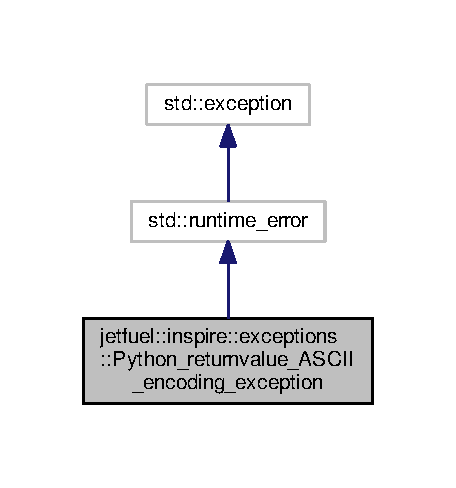
\includegraphics[width=219pt]{classjetfuel_1_1inspire_1_1exceptions_1_1Python__returnvalue__ASCII__encoding__exception__inherit__graph}
\end{center}
\end{figure}


Collaboration diagram for jetfuel\+:\+:inspire\+:\+:exceptions\+:\+:Python\+\_\+returnvalue\+\_\+\+A\+S\+C\+I\+I\+\_\+encoding\+\_\+exception\+:
\nopagebreak
\begin{figure}[H]
\begin{center}
\leavevmode
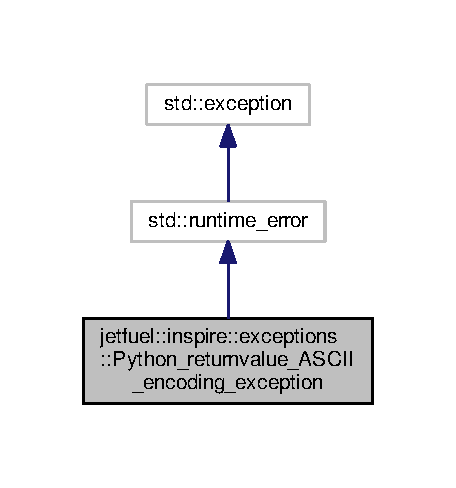
\includegraphics[width=219pt]{classjetfuel_1_1inspire_1_1exceptions_1_1Python__returnvalue__ASCII__encoding__exception__coll__graph}
\end{center}
\end{figure}
\subsection*{Public Member Functions}
\begin{DoxyCompactItemize}
\item 
\mbox{\Hypertarget{classjetfuel_1_1inspire_1_1exceptions_1_1Python__returnvalue__ASCII__encoding__exception_a654d896ec64d3fbb9720e295d52a7f76}\label{classjetfuel_1_1inspire_1_1exceptions_1_1Python__returnvalue__ASCII__encoding__exception_a654d896ec64d3fbb9720e295d52a7f76}} 
{\bfseries Python\+\_\+returnvalue\+\_\+\+A\+S\+C\+I\+I\+\_\+encoding\+\_\+exception} (const std\+::string filename, const std\+::string functionname)
\end{DoxyCompactItemize}


The documentation for this class was generated from the following file\+:\begin{DoxyCompactItemize}
\item 
include/jetfuelinspire/pythonmoduleloader.\+h\end{DoxyCompactItemize}

\hypertarget{classjetfuel_1_1draw_1_1Rect2d}{}\section{jetfuel\+:\+:draw\+:\+:Rect2d$<$ T $>$ Class Template Reference}
\label{classjetfuel_1_1draw_1_1Rect2d}\index{jetfuel\+::draw\+::\+Rect2d$<$ T $>$@{jetfuel\+::draw\+::\+Rect2d$<$ T $>$}}


{\ttfamily \#include $<$rect2d.\+h$>$}

\subsection*{Public Member Functions}
\begin{DoxyCompactItemize}
\item 
\hyperlink{classjetfuel_1_1draw_1_1Rect2d_af5a9c18dea4e196ec326f31ab63ad644}{Rect2d} ()
\begin{DoxyCompactList}\small\item\em Default constructor. \end{DoxyCompactList}\item 
\hyperlink{classjetfuel_1_1draw_1_1Rect2d_aeab9db448df3318ab83fe19f3844f498}{Rect2d} (const T X, const T Y, const T Width, const T Height)
\begin{DoxyCompactList}\small\item\em Constructs a \hyperlink{classjetfuel_1_1draw_1_1Rect2d}{Rect2d} with a x coordinate, a y coordinate, width, and height. \end{DoxyCompactList}\item 
\hyperlink{classjetfuel_1_1draw_1_1Rect2d_ad2cf8c7744252e2202284a230c6d7652}{Rect2d} (const \hyperlink{classjetfuel_1_1draw_1_1Vector2d}{Vector2d}$<$ T $>$ position, const \hyperlink{classjetfuel_1_1draw_1_1Vector2d}{Vector2d}$<$ T $>$ size)
\begin{DoxyCompactList}\small\item\em Constructs a \hyperlink{classjetfuel_1_1draw_1_1Rect2d}{Rect2d} with a position vector, and a size vector. \end{DoxyCompactList}\item 
\hyperlink{classjetfuel_1_1draw_1_1Vector2d}{jetfuel\+::draw\+::\+Vector2d}$<$ T $>$ \hyperlink{classjetfuel_1_1draw_1_1Rect2d_abcc7abd189cc592850484d1314f6220b}{Get\+\_\+position} ()
\begin{DoxyCompactList}\small\item\em Gets the position \hyperlink{classjetfuel_1_1draw_1_1Vector2d}{Vector2d} of the \hyperlink{classjetfuel_1_1draw_1_1Rect2d}{Rect2d}. \end{DoxyCompactList}\item 
\hyperlink{classjetfuel_1_1draw_1_1Vector2d}{jetfuel\+::draw\+::\+Vector2d}$<$ T $>$ \hyperlink{classjetfuel_1_1draw_1_1Rect2d_a3e14b3f59200c452a08085c724950afb}{Get\+\_\+size} ()
\begin{DoxyCompactList}\small\item\em Gets the size \hyperlink{classjetfuel_1_1draw_1_1Vector2d}{Vector2d} of the \hyperlink{classjetfuel_1_1draw_1_1Rect2d}{Rect2d}. \end{DoxyCompactList}\item 
bool \hyperlink{classjetfuel_1_1draw_1_1Rect2d_ae29d8f3e8a6f522d6aacdd00b8d3f757}{Has\+\_\+collided\+\_\+with\+\_\+rect} (\hyperlink{classjetfuel_1_1draw_1_1Rect2d}{jetfuel\+::draw\+::\+Rect2d}$<$ T $>$ rect)
\begin{DoxyCompactList}\small\item\em Detects whether this \hyperlink{classjetfuel_1_1draw_1_1Rect2d}{Rect2d} has collided with another \hyperlink{classjetfuel_1_1draw_1_1Rect2d}{Rect2d} with the same type. \end{DoxyCompactList}\item 
bool \hyperlink{classjetfuel_1_1draw_1_1Rect2d_affa3a06a40154e71485b9676710f6d0d}{Has\+\_\+mouse\+\_\+collided} ()
\begin{DoxyCompactList}\small\item\em Returns whether this \hyperlink{classjetfuel_1_1draw_1_1Rect2d}{Rect2d} has collided with the mouse. \end{DoxyCompactList}\end{DoxyCompactItemize}
\subsection*{Public Attributes}
\begin{DoxyCompactItemize}
\item 
T \hyperlink{classjetfuel_1_1draw_1_1Rect2d_ade151e450d1cc5e7b158a28e7bd6d212}{x}
\begin{DoxyCompactList}\small\item\em member data /// \end{DoxyCompactList}\item 
\mbox{\Hypertarget{classjetfuel_1_1draw_1_1Rect2d_a52d405128b7f28d5427737c3d39cd108}\label{classjetfuel_1_1draw_1_1Rect2d_a52d405128b7f28d5427737c3d39cd108}} 
T \hyperlink{classjetfuel_1_1draw_1_1Rect2d_a52d405128b7f28d5427737c3d39cd108}{y}
\begin{DoxyCompactList}\small\item\em y coordinate \end{DoxyCompactList}\item 
\mbox{\Hypertarget{classjetfuel_1_1draw_1_1Rect2d_aa7e4446e059ed2d85ba66111b1d012f5}\label{classjetfuel_1_1draw_1_1Rect2d_aa7e4446e059ed2d85ba66111b1d012f5}} 
T \hyperlink{classjetfuel_1_1draw_1_1Rect2d_aa7e4446e059ed2d85ba66111b1d012f5}{width}
\begin{DoxyCompactList}\small\item\em width of rectangle \end{DoxyCompactList}\item 
\mbox{\Hypertarget{classjetfuel_1_1draw_1_1Rect2d_afd76834755d8698172922b9d1793f630}\label{classjetfuel_1_1draw_1_1Rect2d_afd76834755d8698172922b9d1793f630}} 
T \hyperlink{classjetfuel_1_1draw_1_1Rect2d_afd76834755d8698172922b9d1793f630}{height}
\begin{DoxyCompactList}\small\item\em height of rectangle \end{DoxyCompactList}\end{DoxyCompactItemize}


\subsection{Detailed Description}
\subsubsection*{template$<$class T$>$\newline
class jetfuel\+::draw\+::\+Rect2d$<$ T $>$}

A simple 2d rectangle manipulation class.

Code Example\+: jetfuel\+::draw\+::\+Rect2d\+\_\+int myrect(0,0,5,5); \hyperlink{classjetfuel_1_1draw_1_1Rectangle__2d__shape}{jetfuel\+::draw\+::\+Rectangle\+\_\+2d\+\_\+shape} mydrawablerect(myrect); \hyperlink{classjetfuel_1_1draw_1_1Scene__manager}{jetfuel\+::draw\+::\+Scene\+\_\+manager} scenemanager; \hyperlink{classjetfuel_1_1draw_1_1Scene}{jetfuel\+::draw\+::\+Scene} scene1(1);

if(!scenemanager.Create\+\_\+window(\char`\"{}example\char`\"{}, jetfuel\+::draw\+::\+Vector2d\+\_\+int(0,0), jetfuel\+::draw\+::\+Vector2d\+\_\+int(500,500)))\{ std\+::cerr $<$$<$ \char`\"{}\mbox{[}!\mbox{]}\+E\+R\+R\+O\+R with creating sdl renderer!\char`\"{} $<$$<$ \char`\"{}\+Error is\+:\char`\"{} $<$$<$ S\+D\+L\+\_\+\+Get\+Error() $<$$<$ \char`\"{}\textbackslash{}n\char`\"{}; \}

if(!scenemanager.Create\+\_\+renderer())\{ std\+::cerr $<$$<$ \char`\"{}\mbox{[}!\mbox{]}\+E\+R\+R\+O\+R with creating sdl renderer!\char`\"{} $<$$<$ \char`\"{}\+Error is\+:\char`\"{} $<$$<$ S\+D\+L\+\_\+\+Get\+Error() $<$$<$ \char`\"{}\textbackslash{}n\char`\"{}; \}

scenemanager.\+Switch\+\_\+current\+\_\+scene(\&scene1);

mydrawablerect.\+Set\+\_\+fill\+\_\+color(jetfuel\+::draw\+::\+Color\+::\+Cyan); scene1.\+Attach\+\_\+drawable(\&mydrawablerect,1\+S);

scenemanager.\+Draw\+\_\+current\+\_\+scene(); 

\subsection{Constructor \& Destructor Documentation}
\mbox{\Hypertarget{classjetfuel_1_1draw_1_1Rect2d_af5a9c18dea4e196ec326f31ab63ad644}\label{classjetfuel_1_1draw_1_1Rect2d_af5a9c18dea4e196ec326f31ab63ad644}} 
\index{jetfuel\+::draw\+::\+Rect2d@{jetfuel\+::draw\+::\+Rect2d}!Rect2d@{Rect2d}}
\index{Rect2d@{Rect2d}!jetfuel\+::draw\+::\+Rect2d@{jetfuel\+::draw\+::\+Rect2d}}
\subsubsection{\texorpdfstring{Rect2d()}{Rect2d()}\hspace{0.1cm}{\footnotesize\ttfamily [1/3]}}
{\footnotesize\ttfamily template$<$class T$>$ \\
\hyperlink{classjetfuel_1_1draw_1_1Rect2d}{jetfuel\+::draw\+::\+Rect2d}$<$ T $>$\+::\hyperlink{classjetfuel_1_1draw_1_1Rect2d}{Rect2d} (\begin{DoxyParamCaption}{ }\end{DoxyParamCaption})\hspace{0.3cm}{\ttfamily [inline]}}



Default constructor. 

Constructs an empty \hyperlink{classjetfuel_1_1draw_1_1Rect2d}{Rect2d} with all values set to 0. \mbox{\Hypertarget{classjetfuel_1_1draw_1_1Rect2d_aeab9db448df3318ab83fe19f3844f498}\label{classjetfuel_1_1draw_1_1Rect2d_aeab9db448df3318ab83fe19f3844f498}} 
\index{jetfuel\+::draw\+::\+Rect2d@{jetfuel\+::draw\+::\+Rect2d}!Rect2d@{Rect2d}}
\index{Rect2d@{Rect2d}!jetfuel\+::draw\+::\+Rect2d@{jetfuel\+::draw\+::\+Rect2d}}
\subsubsection{\texorpdfstring{Rect2d()}{Rect2d()}\hspace{0.1cm}{\footnotesize\ttfamily [2/3]}}
{\footnotesize\ttfamily template$<$class T$>$ \\
\hyperlink{classjetfuel_1_1draw_1_1Rect2d}{jetfuel\+::draw\+::\+Rect2d}$<$ T $>$\+::\hyperlink{classjetfuel_1_1draw_1_1Rect2d}{Rect2d} (\begin{DoxyParamCaption}\item[{const T}]{X,  }\item[{const T}]{Y,  }\item[{const T}]{Width,  }\item[{const T}]{Height }\end{DoxyParamCaption})\hspace{0.3cm}{\ttfamily [inline]}}



Constructs a \hyperlink{classjetfuel_1_1draw_1_1Rect2d}{Rect2d} with a x coordinate, a y coordinate, width, and height. 

Constructs a \hyperlink{classjetfuel_1_1draw_1_1Rect2d}{Rect2d} with a x coordinate, a y coordinate, width, and height.


\begin{DoxyParams}{Parameters}
{\em T} & X \\
\hline
{\em T} & Y \\
\hline
{\em T} & Width \\
\hline
{\em T} & Height \\
\hline
\end{DoxyParams}
\mbox{\Hypertarget{classjetfuel_1_1draw_1_1Rect2d_ad2cf8c7744252e2202284a230c6d7652}\label{classjetfuel_1_1draw_1_1Rect2d_ad2cf8c7744252e2202284a230c6d7652}} 
\index{jetfuel\+::draw\+::\+Rect2d@{jetfuel\+::draw\+::\+Rect2d}!Rect2d@{Rect2d}}
\index{Rect2d@{Rect2d}!jetfuel\+::draw\+::\+Rect2d@{jetfuel\+::draw\+::\+Rect2d}}
\subsubsection{\texorpdfstring{Rect2d()}{Rect2d()}\hspace{0.1cm}{\footnotesize\ttfamily [3/3]}}
{\footnotesize\ttfamily template$<$class T$>$ \\
\hyperlink{classjetfuel_1_1draw_1_1Rect2d}{jetfuel\+::draw\+::\+Rect2d}$<$ T $>$\+::\hyperlink{classjetfuel_1_1draw_1_1Rect2d}{Rect2d} (\begin{DoxyParamCaption}\item[{const \hyperlink{classjetfuel_1_1draw_1_1Vector2d}{Vector2d}$<$ T $>$}]{position,  }\item[{const \hyperlink{classjetfuel_1_1draw_1_1Vector2d}{Vector2d}$<$ T $>$}]{size }\end{DoxyParamCaption})\hspace{0.3cm}{\ttfamily [inline]}}



Constructs a \hyperlink{classjetfuel_1_1draw_1_1Rect2d}{Rect2d} with a position vector, and a size vector. 

Constructs a \hyperlink{classjetfuel_1_1draw_1_1Rect2d}{Rect2d} with a position vector, and a size vector.

jetfuel\+::draw\+::\+Vector2d$<$\+T$>$ position jetfuel\+::draw\+::\+Vector2d$<$\+T$>$ size 

\subsection{Member Function Documentation}
\mbox{\Hypertarget{classjetfuel_1_1draw_1_1Rect2d_abcc7abd189cc592850484d1314f6220b}\label{classjetfuel_1_1draw_1_1Rect2d_abcc7abd189cc592850484d1314f6220b}} 
\index{jetfuel\+::draw\+::\+Rect2d@{jetfuel\+::draw\+::\+Rect2d}!Get\+\_\+position@{Get\+\_\+position}}
\index{Get\+\_\+position@{Get\+\_\+position}!jetfuel\+::draw\+::\+Rect2d@{jetfuel\+::draw\+::\+Rect2d}}
\subsubsection{\texorpdfstring{Get\+\_\+position()}{Get\_position()}}
{\footnotesize\ttfamily template$<$class T$>$ \\
\hyperlink{classjetfuel_1_1draw_1_1Vector2d}{jetfuel\+::draw\+::\+Vector2d}$<$T$>$ \hyperlink{classjetfuel_1_1draw_1_1Rect2d}{jetfuel\+::draw\+::\+Rect2d}$<$ T $>$\+::Get\+\_\+position (\begin{DoxyParamCaption}{ }\end{DoxyParamCaption})\hspace{0.3cm}{\ttfamily [inline]}}



Gets the position \hyperlink{classjetfuel_1_1draw_1_1Vector2d}{Vector2d} of the \hyperlink{classjetfuel_1_1draw_1_1Rect2d}{Rect2d}. 

Gets the position \hyperlink{classjetfuel_1_1draw_1_1Vector2d}{Vector2d} of the \hyperlink{classjetfuel_1_1draw_1_1Rect2d}{Rect2d}. \mbox{\Hypertarget{classjetfuel_1_1draw_1_1Rect2d_a3e14b3f59200c452a08085c724950afb}\label{classjetfuel_1_1draw_1_1Rect2d_a3e14b3f59200c452a08085c724950afb}} 
\index{jetfuel\+::draw\+::\+Rect2d@{jetfuel\+::draw\+::\+Rect2d}!Get\+\_\+size@{Get\+\_\+size}}
\index{Get\+\_\+size@{Get\+\_\+size}!jetfuel\+::draw\+::\+Rect2d@{jetfuel\+::draw\+::\+Rect2d}}
\subsubsection{\texorpdfstring{Get\+\_\+size()}{Get\_size()}}
{\footnotesize\ttfamily template$<$class T$>$ \\
\hyperlink{classjetfuel_1_1draw_1_1Vector2d}{jetfuel\+::draw\+::\+Vector2d}$<$T$>$ \hyperlink{classjetfuel_1_1draw_1_1Rect2d}{jetfuel\+::draw\+::\+Rect2d}$<$ T $>$\+::Get\+\_\+size (\begin{DoxyParamCaption}{ }\end{DoxyParamCaption})\hspace{0.3cm}{\ttfamily [inline]}}



Gets the size \hyperlink{classjetfuel_1_1draw_1_1Vector2d}{Vector2d} of the \hyperlink{classjetfuel_1_1draw_1_1Rect2d}{Rect2d}. 

Gets the size \hyperlink{classjetfuel_1_1draw_1_1Vector2d}{Vector2d} of the \hyperlink{classjetfuel_1_1draw_1_1Rect2d}{Rect2d}. \mbox{\Hypertarget{classjetfuel_1_1draw_1_1Rect2d_ae29d8f3e8a6f522d6aacdd00b8d3f757}\label{classjetfuel_1_1draw_1_1Rect2d_ae29d8f3e8a6f522d6aacdd00b8d3f757}} 
\index{jetfuel\+::draw\+::\+Rect2d@{jetfuel\+::draw\+::\+Rect2d}!Has\+\_\+collided\+\_\+with\+\_\+rect@{Has\+\_\+collided\+\_\+with\+\_\+rect}}
\index{Has\+\_\+collided\+\_\+with\+\_\+rect@{Has\+\_\+collided\+\_\+with\+\_\+rect}!jetfuel\+::draw\+::\+Rect2d@{jetfuel\+::draw\+::\+Rect2d}}
\subsubsection{\texorpdfstring{Has\+\_\+collided\+\_\+with\+\_\+rect()}{Has\_collided\_with\_rect()}}
{\footnotesize\ttfamily template$<$class T$>$ \\
bool \hyperlink{classjetfuel_1_1draw_1_1Rect2d}{jetfuel\+::draw\+::\+Rect2d}$<$ T $>$\+::Has\+\_\+collided\+\_\+with\+\_\+rect (\begin{DoxyParamCaption}\item[{\hyperlink{classjetfuel_1_1draw_1_1Rect2d}{jetfuel\+::draw\+::\+Rect2d}$<$ T $>$}]{rect }\end{DoxyParamCaption})\hspace{0.3cm}{\ttfamily [inline]}}



Detects whether this \hyperlink{classjetfuel_1_1draw_1_1Rect2d}{Rect2d} has collided with another \hyperlink{classjetfuel_1_1draw_1_1Rect2d}{Rect2d} with the same type. 

Detects whether this \hyperlink{classjetfuel_1_1draw_1_1Rect2d}{Rect2d} has collided with another \hyperlink{classjetfuel_1_1draw_1_1Rect2d}{Rect2d} with the same type.


\begin{DoxyParams}{Parameters}
{\em Rect2d$<$\+T$>$} & \\
\hline
\end{DoxyParams}
\mbox{\Hypertarget{classjetfuel_1_1draw_1_1Rect2d_affa3a06a40154e71485b9676710f6d0d}\label{classjetfuel_1_1draw_1_1Rect2d_affa3a06a40154e71485b9676710f6d0d}} 
\index{jetfuel\+::draw\+::\+Rect2d@{jetfuel\+::draw\+::\+Rect2d}!Has\+\_\+mouse\+\_\+collided@{Has\+\_\+mouse\+\_\+collided}}
\index{Has\+\_\+mouse\+\_\+collided@{Has\+\_\+mouse\+\_\+collided}!jetfuel\+::draw\+::\+Rect2d@{jetfuel\+::draw\+::\+Rect2d}}
\subsubsection{\texorpdfstring{Has\+\_\+mouse\+\_\+collided()}{Has\_mouse\_collided()}}
{\footnotesize\ttfamily template$<$class T$>$ \\
bool \hyperlink{classjetfuel_1_1draw_1_1Rect2d}{jetfuel\+::draw\+::\+Rect2d}$<$ T $>$\+::Has\+\_\+mouse\+\_\+collided (\begin{DoxyParamCaption}{ }\end{DoxyParamCaption})\hspace{0.3cm}{\ttfamily [inline]}}



Returns whether this \hyperlink{classjetfuel_1_1draw_1_1Rect2d}{Rect2d} has collided with the mouse. 

Returns whether this \hyperlink{classjetfuel_1_1draw_1_1Rect2d}{Rect2d} has collided with the mouse. 

\subsection{Member Data Documentation}
\mbox{\Hypertarget{classjetfuel_1_1draw_1_1Rect2d_ade151e450d1cc5e7b158a28e7bd6d212}\label{classjetfuel_1_1draw_1_1Rect2d_ade151e450d1cc5e7b158a28e7bd6d212}} 
\index{jetfuel\+::draw\+::\+Rect2d@{jetfuel\+::draw\+::\+Rect2d}!x@{x}}
\index{x@{x}!jetfuel\+::draw\+::\+Rect2d@{jetfuel\+::draw\+::\+Rect2d}}
\subsubsection{\texorpdfstring{x}{x}}
{\footnotesize\ttfamily template$<$class T$>$ \\
T \hyperlink{classjetfuel_1_1draw_1_1Rect2d}{jetfuel\+::draw\+::\+Rect2d}$<$ T $>$\+::x}



member data /// 

x coordinate 

The documentation for this class was generated from the following file\+:\begin{DoxyCompactItemize}
\item 
include/jetfueldraw/rect2d.\+h\end{DoxyCompactItemize}

\hypertarget{classjetfuel_1_1draw_1_1Rectangle__2d__shape}{}\section{jetfuel\+:\+:draw\+:\+:Rectangle\+\_\+2d\+\_\+shape Class Reference}
\label{classjetfuel_1_1draw_1_1Rectangle__2d__shape}\index{jetfuel\+::draw\+::\+Rectangle\+\_\+2d\+\_\+shape@{jetfuel\+::draw\+::\+Rectangle\+\_\+2d\+\_\+shape}}


{\ttfamily \#include $<$rectangle2dshape.\+h$>$}



Inheritance diagram for jetfuel\+:\+:draw\+:\+:Rectangle\+\_\+2d\+\_\+shape\+:
\nopagebreak
\begin{figure}[H]
\begin{center}
\leavevmode
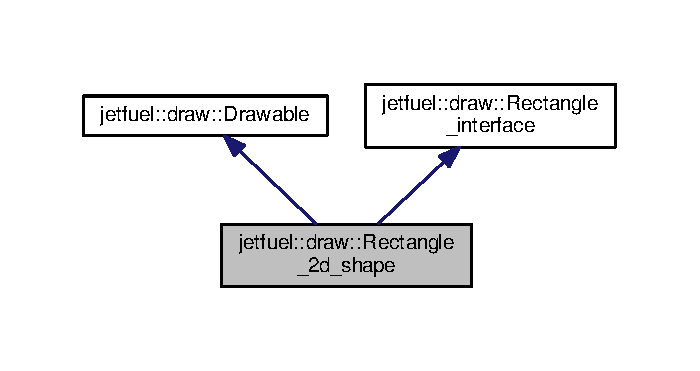
\includegraphics[width=336pt]{classjetfuel_1_1draw_1_1Rectangle__2d__shape__inherit__graph}
\end{center}
\end{figure}


Collaboration diagram for jetfuel\+:\+:draw\+:\+:Rectangle\+\_\+2d\+\_\+shape\+:
\nopagebreak
\begin{figure}[H]
\begin{center}
\leavevmode
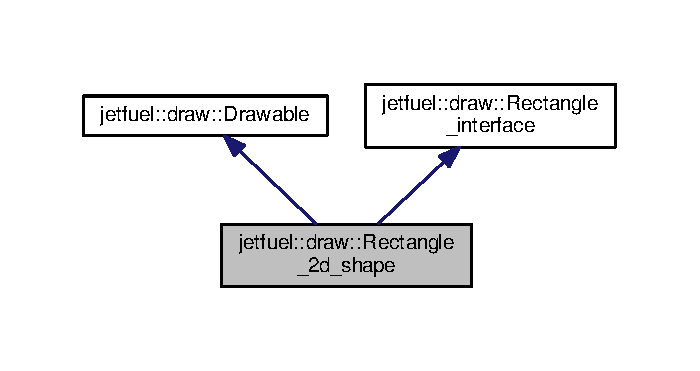
\includegraphics[width=336pt]{classjetfuel_1_1draw_1_1Rectangle__2d__shape__coll__graph}
\end{center}
\end{figure}
\subsection*{Classes}
\begin{DoxyCompactItemize}
\item 
struct \hyperlink{structjetfuel_1_1draw_1_1Rectangle__2d__shape_1_1Rectangle__2d__shape__characteristics}{Rectangle\+\_\+2d\+\_\+shape\+\_\+characteristics}
\end{DoxyCompactItemize}
\subsection*{Public Member Functions}
\begin{DoxyCompactItemize}
\item 
\hyperlink{classjetfuel_1_1draw_1_1Rectangle__2d__shape_a4ee9006d8e9d043092eff698ab484210}{Rectangle\+\_\+2d\+\_\+shape} (\hyperlink{classjetfuel_1_1draw_1_1Vector2d}{Vector2d\+\_\+int} position, \hyperlink{classjetfuel_1_1draw_1_1Vector2d}{Vector2d\+\_\+int} size)
\begin{DoxyCompactList}\small\item\em Constructs the \hyperlink{classjetfuel_1_1draw_1_1Rectangle__2d__shape}{Rectangle\+\_\+2d\+\_\+shape} with a position \hyperlink{classjetfuel_1_1draw_1_1Vector2d}{Vector2d} and a size \hyperlink{classjetfuel_1_1draw_1_1Vector2d}{Vector2d}. \end{DoxyCompactList}\item 
\hyperlink{classjetfuel_1_1draw_1_1Rectangle__2d__shape_a5b75e1dc1fe55ecf69b551888d78e352}{Rectangle\+\_\+2d\+\_\+shape} (\hyperlink{classjetfuel_1_1draw_1_1Rect2d}{Rect2d\+\_\+int} rect)
\begin{DoxyCompactList}\small\item\em Constructs the \hyperlink{classjetfuel_1_1draw_1_1Rectangle__2d__shape}{Rectangle\+\_\+2d\+\_\+shape} with a \hyperlink{classjetfuel_1_1draw_1_1Rect2d}{Rect2d}. \end{DoxyCompactList}\item 
\hyperlink{classjetfuel_1_1draw_1_1Color}{Color} \hyperlink{classjetfuel_1_1draw_1_1Rectangle__2d__shape_a87340a4dcdcdc3b4d3aa059b5fe4c3af}{Get\+\_\+fill\+\_\+color} () const
\begin{DoxyCompactList}\small\item\em Returns the fill color of the rectangle. \end{DoxyCompactList}\item 
void \hyperlink{classjetfuel_1_1draw_1_1Rectangle__2d__shape_a2dfd78b34c5d1742ca2e41b86c7f9d12}{Set\+\_\+fill\+\_\+color} (const \hyperlink{classjetfuel_1_1draw_1_1Color}{Color} rectcolor)
\begin{DoxyCompactList}\small\item\em Sets the fill color of the rectangle. \end{DoxyCompactList}\item 
\hyperlink{classjetfuel_1_1draw_1_1Vector2d}{jetfuel\+::draw\+::\+Vector2d\+\_\+int} \hyperlink{classjetfuel_1_1draw_1_1Rectangle__2d__shape_ace7c296b14b0ad8f15e6ed1115000b1e}{Get\+\_\+size} ()
\begin{DoxyCompactList}\small\item\em Gets the size \hyperlink{classjetfuel_1_1draw_1_1Vector2d}{Vector2d} of the \hyperlink{classjetfuel_1_1draw_1_1Rectangle__2d__shape}{Rectangle\+\_\+2d\+\_\+shape}. \end{DoxyCompactList}\item 
void \hyperlink{classjetfuel_1_1draw_1_1Rectangle__2d__shape_a27f242564a455d5cd7274e50e5156ffc}{Set\+\_\+size} (const \hyperlink{classjetfuel_1_1draw_1_1Vector2d}{Vector2d\+\_\+int} size)
\begin{DoxyCompactList}\small\item\em Sets the size \hyperlink{classjetfuel_1_1draw_1_1Vector2d}{Vector2d} of the \hyperlink{classjetfuel_1_1draw_1_1Rectangle__2d__shape}{Rectangle\+\_\+2d\+\_\+shape}. \end{DoxyCompactList}\item 
\hyperlink{classjetfuel_1_1draw_1_1Vector2d}{jetfuel\+::draw\+::\+Vector2d\+\_\+int} \hyperlink{classjetfuel_1_1draw_1_1Rectangle__2d__shape_a60aa3e0fa050e3fbd98177c1eef721b0}{Get\+\_\+position} () override
\begin{DoxyCompactList}\small\item\em Gets the position \hyperlink{classjetfuel_1_1draw_1_1Vector2d}{Vector2d} of the \hyperlink{classjetfuel_1_1draw_1_1Rectangle__2d__shape}{Rectangle\+\_\+2d\+\_\+shape}. \end{DoxyCompactList}\item 
void \hyperlink{classjetfuel_1_1draw_1_1Rectangle__2d__shape_a375b0892589ef7cd1762576e9ce96875}{Set\+\_\+position} (const \hyperlink{classjetfuel_1_1draw_1_1Vector2d}{Vector2d\+\_\+int} position) override
\begin{DoxyCompactList}\small\item\em Sets the position \hyperlink{classjetfuel_1_1draw_1_1Vector2d}{Vector2d} of the \hyperlink{classjetfuel_1_1draw_1_1Rectangle__2d__shape}{Rectangle\+\_\+2d\+\_\+shape}. \end{DoxyCompactList}\item 
\hyperlink{classjetfuel_1_1draw_1_1Color}{Color} \hyperlink{classjetfuel_1_1draw_1_1Rectangle__2d__shape_a63a682ca90cc17cc993253757296c999}{Get\+\_\+outline\+\_\+color} () const
\begin{DoxyCompactList}\small\item\em Returns the outline color of the rectangle. \end{DoxyCompactList}\item 
void \hyperlink{classjetfuel_1_1draw_1_1Rectangle__2d__shape_a7a090088081738c7f342e193e519de5a}{Set\+\_\+outline\+\_\+color} (const \hyperlink{classjetfuel_1_1draw_1_1Color}{Color} rectcolor)
\begin{DoxyCompactList}\small\item\em Sets the outline color of the rectangle. \end{DoxyCompactList}\item 
void \hyperlink{classjetfuel_1_1draw_1_1Rectangle__2d__shape_a505b8a9c99a2a552d680d7fa1a7622d9}{Disable\+\_\+drawing\+\_\+outline\+\_\+color} ()
\begin{DoxyCompactList}\small\item\em Disables drawing the outline color enabled by Set\+\_\+outline\+\_\+color. \end{DoxyCompactList}\item 
\hyperlink{classjetfuel_1_1draw_1_1Rect2d}{Rect2d\+\_\+int} \hyperlink{classjetfuel_1_1draw_1_1Rectangle__2d__shape_a1ed2975565e629d2b8d3fffa0a4756b2}{Get\+\_\+rect\+\_\+to\+\_\+draw} () override
\begin{DoxyCompactList}\small\item\em Returns the \hyperlink{classjetfuel_1_1draw_1_1Rect2d}{Rect2d} to be drawn. \end{DoxyCompactList}\item 
bool \hyperlink{classjetfuel_1_1draw_1_1Rectangle__2d__shape_aba19e63d55c824de135932483fe40fcb}{Draw} () override
\begin{DoxyCompactList}\small\item\em Draws the rectangle. \end{DoxyCompactList}\end{DoxyCompactItemize}
\subsection*{Protected Member Functions}
\begin{DoxyCompactItemize}
\item 
bool \hyperlink{classjetfuel_1_1draw_1_1Rectangle__2d__shape_a10cb5ef4b0d1b10b9d1b1bf32a805613}{Is\+\_\+draw\+\_\+outline} () const
\begin{DoxyCompactList}\small\item\em Returns whether this class is drawing an outline. \end{DoxyCompactList}\end{DoxyCompactItemize}


\subsection{Detailed Description}
A 2d rectangle that can be drawn to the player.

Code Example\+: \hyperlink{classjetfuel_1_1draw_1_1Scene__manager}{jetfuel\+::draw\+::\+Scene\+\_\+manager} scenemanager; \hyperlink{classjetfuel_1_1draw_1_1Scene}{jetfuel\+::draw\+::\+Scene} scene1(1); \hyperlink{classjetfuel_1_1draw_1_1Rectangle__2d__shape}{jetfuel\+::draw\+::\+Rectangle\+\_\+2d\+\_\+shape} rect( jetfuel\+::draw\+::\+Rect2d\+\_\+int(100,100,400,400));

if(!scenemanager.Create\+\_\+window(\char`\"{}example\char`\"{}, jetfuel\+::draw\+::\+Vector2d\+\_\+int(0,0), jetfuel\+::draw\+::\+Vector2d\+\_\+int(500,500)))\{ std\+::cerr $<$$<$ \char`\"{}\mbox{[}!\mbox{]}\+E\+R\+R\+O\+R with creating sdl renderer!\char`\"{} $<$$<$ \char`\"{}\+Error is\+:\char`\"{} $<$$<$ S\+D\+L\+\_\+\+Get\+Error() $<$$<$ \char`\"{}\textbackslash{}n\char`\"{}; \}

if(!scenemanager.Create\+\_\+renderer())\{ std\+::cerr $<$$<$ \char`\"{}\mbox{[}!\mbox{]}\+E\+R\+R\+O\+R with creating sdl renderer!\char`\"{} $<$$<$ \char`\"{}\+Error is\+:\char`\"{} $<$$<$ S\+D\+L\+\_\+\+Get\+Error() $<$$<$ \char`\"{}\textbackslash{}n\char`\"{}; \}

scenemanager.\+Switch\+\_\+current\+\_\+scene(\&scene1);

rect.\+Set\+\_\+fill\+\_\+color(jetfuel\+::draw\+::\+Color\+::\+Magenta); scene1.\+Attach\+\_\+drawable(\&rect,2);

scenemanager.\+Draw\+\_\+current\+\_\+scene(); 

\subsection{Constructor \& Destructor Documentation}
\mbox{\Hypertarget{classjetfuel_1_1draw_1_1Rectangle__2d__shape_a4ee9006d8e9d043092eff698ab484210}\label{classjetfuel_1_1draw_1_1Rectangle__2d__shape_a4ee9006d8e9d043092eff698ab484210}} 
\index{jetfuel\+::draw\+::\+Rectangle\+\_\+2d\+\_\+shape@{jetfuel\+::draw\+::\+Rectangle\+\_\+2d\+\_\+shape}!Rectangle\+\_\+2d\+\_\+shape@{Rectangle\+\_\+2d\+\_\+shape}}
\index{Rectangle\+\_\+2d\+\_\+shape@{Rectangle\+\_\+2d\+\_\+shape}!jetfuel\+::draw\+::\+Rectangle\+\_\+2d\+\_\+shape@{jetfuel\+::draw\+::\+Rectangle\+\_\+2d\+\_\+shape}}
\subsubsection{\texorpdfstring{Rectangle\+\_\+2d\+\_\+shape()}{Rectangle\_2d\_shape()}\hspace{0.1cm}{\footnotesize\ttfamily [1/2]}}
{\footnotesize\ttfamily jetfuel\+::draw\+::\+Rectangle\+\_\+2d\+\_\+shape\+::\+Rectangle\+\_\+2d\+\_\+shape (\begin{DoxyParamCaption}\item[{\hyperlink{classjetfuel_1_1draw_1_1Vector2d}{Vector2d\+\_\+int}}]{position,  }\item[{\hyperlink{classjetfuel_1_1draw_1_1Vector2d}{Vector2d\+\_\+int}}]{size }\end{DoxyParamCaption})}



Constructs the \hyperlink{classjetfuel_1_1draw_1_1Rectangle__2d__shape}{Rectangle\+\_\+2d\+\_\+shape} with a position \hyperlink{classjetfuel_1_1draw_1_1Vector2d}{Vector2d} and a size \hyperlink{classjetfuel_1_1draw_1_1Vector2d}{Vector2d}. 

Constructs the \hyperlink{classjetfuel_1_1draw_1_1Rectangle__2d__shape}{Rectangle\+\_\+2d\+\_\+shape} object with a position \hyperlink{classjetfuel_1_1draw_1_1Vector2d}{Vector2d} and a size \hyperlink{classjetfuel_1_1draw_1_1Vector2d}{Vector2d} of the rectangle.


\begin{DoxyParams}{Parameters}
{\em jetfuel\+::draw\+::\+Vector2d\+\_\+int} & position \\
\hline
{\em jetfuel\+::draw\+::\+Vector2d\+\_\+int} & size \\
\hline
\end{DoxyParams}
\mbox{\Hypertarget{classjetfuel_1_1draw_1_1Rectangle__2d__shape_a5b75e1dc1fe55ecf69b551888d78e352}\label{classjetfuel_1_1draw_1_1Rectangle__2d__shape_a5b75e1dc1fe55ecf69b551888d78e352}} 
\index{jetfuel\+::draw\+::\+Rectangle\+\_\+2d\+\_\+shape@{jetfuel\+::draw\+::\+Rectangle\+\_\+2d\+\_\+shape}!Rectangle\+\_\+2d\+\_\+shape@{Rectangle\+\_\+2d\+\_\+shape}}
\index{Rectangle\+\_\+2d\+\_\+shape@{Rectangle\+\_\+2d\+\_\+shape}!jetfuel\+::draw\+::\+Rectangle\+\_\+2d\+\_\+shape@{jetfuel\+::draw\+::\+Rectangle\+\_\+2d\+\_\+shape}}
\subsubsection{\texorpdfstring{Rectangle\+\_\+2d\+\_\+shape()}{Rectangle\_2d\_shape()}\hspace{0.1cm}{\footnotesize\ttfamily [2/2]}}
{\footnotesize\ttfamily jetfuel\+::draw\+::\+Rectangle\+\_\+2d\+\_\+shape\+::\+Rectangle\+\_\+2d\+\_\+shape (\begin{DoxyParamCaption}\item[{\hyperlink{classjetfuel_1_1draw_1_1Rect2d}{Rect2d\+\_\+int}}]{rect }\end{DoxyParamCaption})}



Constructs the \hyperlink{classjetfuel_1_1draw_1_1Rectangle__2d__shape}{Rectangle\+\_\+2d\+\_\+shape} with a \hyperlink{classjetfuel_1_1draw_1_1Rect2d}{Rect2d}. 

Constructs the \hyperlink{classjetfuel_1_1draw_1_1Rectangle__2d__shape}{Rectangle\+\_\+2d\+\_\+shape} object with a \hyperlink{classjetfuel_1_1draw_1_1Rect2d}{Rect2d}.


\begin{DoxyParams}{Parameters}
{\em jetfuel\+::draw\+::\+Rect2d\+\_\+int} & rect \\
\hline
\end{DoxyParams}


\subsection{Member Function Documentation}
\mbox{\Hypertarget{classjetfuel_1_1draw_1_1Rectangle__2d__shape_a505b8a9c99a2a552d680d7fa1a7622d9}\label{classjetfuel_1_1draw_1_1Rectangle__2d__shape_a505b8a9c99a2a552d680d7fa1a7622d9}} 
\index{jetfuel\+::draw\+::\+Rectangle\+\_\+2d\+\_\+shape@{jetfuel\+::draw\+::\+Rectangle\+\_\+2d\+\_\+shape}!Disable\+\_\+drawing\+\_\+outline\+\_\+color@{Disable\+\_\+drawing\+\_\+outline\+\_\+color}}
\index{Disable\+\_\+drawing\+\_\+outline\+\_\+color@{Disable\+\_\+drawing\+\_\+outline\+\_\+color}!jetfuel\+::draw\+::\+Rectangle\+\_\+2d\+\_\+shape@{jetfuel\+::draw\+::\+Rectangle\+\_\+2d\+\_\+shape}}
\subsubsection{\texorpdfstring{Disable\+\_\+drawing\+\_\+outline\+\_\+color()}{Disable\_drawing\_outline\_color()}}
{\footnotesize\ttfamily void jetfuel\+::draw\+::\+Rectangle\+\_\+2d\+\_\+shape\+::\+Disable\+\_\+drawing\+\_\+outline\+\_\+color (\begin{DoxyParamCaption}{ }\end{DoxyParamCaption})\hspace{0.3cm}{\ttfamily [inline]}}



Disables drawing the outline color enabled by Set\+\_\+outline\+\_\+color. 

Disables drawing the outline color enabled by the Set\+\_\+outline\+\_\+color function. \mbox{\Hypertarget{classjetfuel_1_1draw_1_1Rectangle__2d__shape_aba19e63d55c824de135932483fe40fcb}\label{classjetfuel_1_1draw_1_1Rectangle__2d__shape_aba19e63d55c824de135932483fe40fcb}} 
\index{jetfuel\+::draw\+::\+Rectangle\+\_\+2d\+\_\+shape@{jetfuel\+::draw\+::\+Rectangle\+\_\+2d\+\_\+shape}!Draw@{Draw}}
\index{Draw@{Draw}!jetfuel\+::draw\+::\+Rectangle\+\_\+2d\+\_\+shape@{jetfuel\+::draw\+::\+Rectangle\+\_\+2d\+\_\+shape}}
\subsubsection{\texorpdfstring{Draw()}{Draw()}}
{\footnotesize\ttfamily bool jetfuel\+::draw\+::\+Rectangle\+\_\+2d\+\_\+shape\+::\+Draw (\begin{DoxyParamCaption}{ }\end{DoxyParamCaption})\hspace{0.3cm}{\ttfamily [override]}, {\ttfamily [virtual]}}



Draws the rectangle. 

Draws the rectangle. It is recommended to let \hyperlink{classjetfuel_1_1draw_1_1Scene}{jetfuel\+::draw\+::\+Scene} and \hyperlink{classjetfuel_1_1draw_1_1Scene__manager}{jetfuel\+::draw\+::\+Scene\+\_\+manager} call this, and not by yourself. 

Implements \hyperlink{classjetfuel_1_1draw_1_1Drawable_a1a072070322965ce9411ee6e7c311c56}{jetfuel\+::draw\+::\+Drawable}.

\mbox{\Hypertarget{classjetfuel_1_1draw_1_1Rectangle__2d__shape_a87340a4dcdcdc3b4d3aa059b5fe4c3af}\label{classjetfuel_1_1draw_1_1Rectangle__2d__shape_a87340a4dcdcdc3b4d3aa059b5fe4c3af}} 
\index{jetfuel\+::draw\+::\+Rectangle\+\_\+2d\+\_\+shape@{jetfuel\+::draw\+::\+Rectangle\+\_\+2d\+\_\+shape}!Get\+\_\+fill\+\_\+color@{Get\+\_\+fill\+\_\+color}}
\index{Get\+\_\+fill\+\_\+color@{Get\+\_\+fill\+\_\+color}!jetfuel\+::draw\+::\+Rectangle\+\_\+2d\+\_\+shape@{jetfuel\+::draw\+::\+Rectangle\+\_\+2d\+\_\+shape}}
\subsubsection{\texorpdfstring{Get\+\_\+fill\+\_\+color()}{Get\_fill\_color()}}
{\footnotesize\ttfamily \hyperlink{classjetfuel_1_1draw_1_1Color}{Color} jetfuel\+::draw\+::\+Rectangle\+\_\+2d\+\_\+shape\+::\+Get\+\_\+fill\+\_\+color (\begin{DoxyParamCaption}{ }\end{DoxyParamCaption}) const\hspace{0.3cm}{\ttfamily [inline]}}



Returns the fill color of the rectangle. 

Returns the fill color of the rectangle. \mbox{\Hypertarget{classjetfuel_1_1draw_1_1Rectangle__2d__shape_a63a682ca90cc17cc993253757296c999}\label{classjetfuel_1_1draw_1_1Rectangle__2d__shape_a63a682ca90cc17cc993253757296c999}} 
\index{jetfuel\+::draw\+::\+Rectangle\+\_\+2d\+\_\+shape@{jetfuel\+::draw\+::\+Rectangle\+\_\+2d\+\_\+shape}!Get\+\_\+outline\+\_\+color@{Get\+\_\+outline\+\_\+color}}
\index{Get\+\_\+outline\+\_\+color@{Get\+\_\+outline\+\_\+color}!jetfuel\+::draw\+::\+Rectangle\+\_\+2d\+\_\+shape@{jetfuel\+::draw\+::\+Rectangle\+\_\+2d\+\_\+shape}}
\subsubsection{\texorpdfstring{Get\+\_\+outline\+\_\+color()}{Get\_outline\_color()}}
{\footnotesize\ttfamily \hyperlink{classjetfuel_1_1draw_1_1Color}{Color} jetfuel\+::draw\+::\+Rectangle\+\_\+2d\+\_\+shape\+::\+Get\+\_\+outline\+\_\+color (\begin{DoxyParamCaption}{ }\end{DoxyParamCaption}) const\hspace{0.3cm}{\ttfamily [inline]}}



Returns the outline color of the rectangle. 

Returns the outline color of the rectangle. \mbox{\Hypertarget{classjetfuel_1_1draw_1_1Rectangle__2d__shape_a60aa3e0fa050e3fbd98177c1eef721b0}\label{classjetfuel_1_1draw_1_1Rectangle__2d__shape_a60aa3e0fa050e3fbd98177c1eef721b0}} 
\index{jetfuel\+::draw\+::\+Rectangle\+\_\+2d\+\_\+shape@{jetfuel\+::draw\+::\+Rectangle\+\_\+2d\+\_\+shape}!Get\+\_\+position@{Get\+\_\+position}}
\index{Get\+\_\+position@{Get\+\_\+position}!jetfuel\+::draw\+::\+Rectangle\+\_\+2d\+\_\+shape@{jetfuel\+::draw\+::\+Rectangle\+\_\+2d\+\_\+shape}}
\subsubsection{\texorpdfstring{Get\+\_\+position()}{Get\_position()}}
{\footnotesize\ttfamily \hyperlink{classjetfuel_1_1draw_1_1Vector2d}{jetfuel\+::draw\+::\+Vector2d\+\_\+int} jetfuel\+::draw\+::\+Rectangle\+\_\+2d\+\_\+shape\+::\+Get\+\_\+position (\begin{DoxyParamCaption}{ }\end{DoxyParamCaption})\hspace{0.3cm}{\ttfamily [inline]}, {\ttfamily [override]}, {\ttfamily [virtual]}}



Gets the position \hyperlink{classjetfuel_1_1draw_1_1Vector2d}{Vector2d} of the \hyperlink{classjetfuel_1_1draw_1_1Rectangle__2d__shape}{Rectangle\+\_\+2d\+\_\+shape}. 

Gets the position \hyperlink{classjetfuel_1_1draw_1_1Vector2d}{Vector2d} of the \hyperlink{classjetfuel_1_1draw_1_1Rectangle__2d__shape}{Rectangle\+\_\+2d\+\_\+shape}. 

Reimplemented from \hyperlink{classjetfuel_1_1draw_1_1Drawable_ae7ebd30d66db2c8a5d5371cbcf0023fc}{jetfuel\+::draw\+::\+Drawable}.

\mbox{\Hypertarget{classjetfuel_1_1draw_1_1Rectangle__2d__shape_a1ed2975565e629d2b8d3fffa0a4756b2}\label{classjetfuel_1_1draw_1_1Rectangle__2d__shape_a1ed2975565e629d2b8d3fffa0a4756b2}} 
\index{jetfuel\+::draw\+::\+Rectangle\+\_\+2d\+\_\+shape@{jetfuel\+::draw\+::\+Rectangle\+\_\+2d\+\_\+shape}!Get\+\_\+rect\+\_\+to\+\_\+draw@{Get\+\_\+rect\+\_\+to\+\_\+draw}}
\index{Get\+\_\+rect\+\_\+to\+\_\+draw@{Get\+\_\+rect\+\_\+to\+\_\+draw}!jetfuel\+::draw\+::\+Rectangle\+\_\+2d\+\_\+shape@{jetfuel\+::draw\+::\+Rectangle\+\_\+2d\+\_\+shape}}
\subsubsection{\texorpdfstring{Get\+\_\+rect\+\_\+to\+\_\+draw()}{Get\_rect\_to\_draw()}}
{\footnotesize\ttfamily \hyperlink{classjetfuel_1_1draw_1_1Rect2d}{Rect2d\+\_\+int} jetfuel\+::draw\+::\+Rectangle\+\_\+2d\+\_\+shape\+::\+Get\+\_\+rect\+\_\+to\+\_\+draw (\begin{DoxyParamCaption}{ }\end{DoxyParamCaption})\hspace{0.3cm}{\ttfamily [inline]}, {\ttfamily [override]}, {\ttfamily [virtual]}}



Returns the \hyperlink{classjetfuel_1_1draw_1_1Rect2d}{Rect2d} to be drawn. 

Returns the \hyperlink{classjetfuel_1_1draw_1_1Rect2d}{jetfuel\+::draw\+::\+Rect2d} to be drawn when the function \hyperlink{classjetfuel_1_1draw_1_1Rectangle__2d__shape_aba19e63d55c824de135932483fe40fcb}{Draw()} is called. 

Implements \hyperlink{classjetfuel_1_1draw_1_1Rectangle__interface_a03fd3b6842ab7b3065379caec407296f}{jetfuel\+::draw\+::\+Rectangle\+\_\+interface}.

\mbox{\Hypertarget{classjetfuel_1_1draw_1_1Rectangle__2d__shape_ace7c296b14b0ad8f15e6ed1115000b1e}\label{classjetfuel_1_1draw_1_1Rectangle__2d__shape_ace7c296b14b0ad8f15e6ed1115000b1e}} 
\index{jetfuel\+::draw\+::\+Rectangle\+\_\+2d\+\_\+shape@{jetfuel\+::draw\+::\+Rectangle\+\_\+2d\+\_\+shape}!Get\+\_\+size@{Get\+\_\+size}}
\index{Get\+\_\+size@{Get\+\_\+size}!jetfuel\+::draw\+::\+Rectangle\+\_\+2d\+\_\+shape@{jetfuel\+::draw\+::\+Rectangle\+\_\+2d\+\_\+shape}}
\subsubsection{\texorpdfstring{Get\+\_\+size()}{Get\_size()}}
{\footnotesize\ttfamily \hyperlink{classjetfuel_1_1draw_1_1Vector2d}{jetfuel\+::draw\+::\+Vector2d\+\_\+int} jetfuel\+::draw\+::\+Rectangle\+\_\+2d\+\_\+shape\+::\+Get\+\_\+size (\begin{DoxyParamCaption}{ }\end{DoxyParamCaption})\hspace{0.3cm}{\ttfamily [inline]}}



Gets the size \hyperlink{classjetfuel_1_1draw_1_1Vector2d}{Vector2d} of the \hyperlink{classjetfuel_1_1draw_1_1Rectangle__2d__shape}{Rectangle\+\_\+2d\+\_\+shape}. 

Gets the size \hyperlink{classjetfuel_1_1draw_1_1Vector2d}{Vector2d} of the \hyperlink{classjetfuel_1_1draw_1_1Rectangle__2d__shape}{Rectangle\+\_\+2d\+\_\+shape}. \mbox{\Hypertarget{classjetfuel_1_1draw_1_1Rectangle__2d__shape_a10cb5ef4b0d1b10b9d1b1bf32a805613}\label{classjetfuel_1_1draw_1_1Rectangle__2d__shape_a10cb5ef4b0d1b10b9d1b1bf32a805613}} 
\index{jetfuel\+::draw\+::\+Rectangle\+\_\+2d\+\_\+shape@{jetfuel\+::draw\+::\+Rectangle\+\_\+2d\+\_\+shape}!Is\+\_\+draw\+\_\+outline@{Is\+\_\+draw\+\_\+outline}}
\index{Is\+\_\+draw\+\_\+outline@{Is\+\_\+draw\+\_\+outline}!jetfuel\+::draw\+::\+Rectangle\+\_\+2d\+\_\+shape@{jetfuel\+::draw\+::\+Rectangle\+\_\+2d\+\_\+shape}}
\subsubsection{\texorpdfstring{Is\+\_\+draw\+\_\+outline()}{Is\_draw\_outline()}}
{\footnotesize\ttfamily bool jetfuel\+::draw\+::\+Rectangle\+\_\+2d\+\_\+shape\+::\+Is\+\_\+draw\+\_\+outline (\begin{DoxyParamCaption}{ }\end{DoxyParamCaption}) const\hspace{0.3cm}{\ttfamily [inline]}, {\ttfamily [protected]}}



Returns whether this class is drawing an outline. 

Returns whether this class is drawing a rectangle outline. \mbox{\Hypertarget{classjetfuel_1_1draw_1_1Rectangle__2d__shape_a2dfd78b34c5d1742ca2e41b86c7f9d12}\label{classjetfuel_1_1draw_1_1Rectangle__2d__shape_a2dfd78b34c5d1742ca2e41b86c7f9d12}} 
\index{jetfuel\+::draw\+::\+Rectangle\+\_\+2d\+\_\+shape@{jetfuel\+::draw\+::\+Rectangle\+\_\+2d\+\_\+shape}!Set\+\_\+fill\+\_\+color@{Set\+\_\+fill\+\_\+color}}
\index{Set\+\_\+fill\+\_\+color@{Set\+\_\+fill\+\_\+color}!jetfuel\+::draw\+::\+Rectangle\+\_\+2d\+\_\+shape@{jetfuel\+::draw\+::\+Rectangle\+\_\+2d\+\_\+shape}}
\subsubsection{\texorpdfstring{Set\+\_\+fill\+\_\+color()}{Set\_fill\_color()}}
{\footnotesize\ttfamily void jetfuel\+::draw\+::\+Rectangle\+\_\+2d\+\_\+shape\+::\+Set\+\_\+fill\+\_\+color (\begin{DoxyParamCaption}\item[{const \hyperlink{classjetfuel_1_1draw_1_1Color}{Color}}]{rectcolor }\end{DoxyParamCaption})\hspace{0.3cm}{\ttfamily [inline]}}



Sets the fill color of the rectangle. 

Sets the fill color of the rectangle.


\begin{DoxyParams}{Parameters}
{\em \hyperlink{classjetfuel_1_1draw_1_1Color}{jetfuel\+::draw\+::\+Color}} & rectcolor \\
\hline
\end{DoxyParams}
\mbox{\Hypertarget{classjetfuel_1_1draw_1_1Rectangle__2d__shape_a7a090088081738c7f342e193e519de5a}\label{classjetfuel_1_1draw_1_1Rectangle__2d__shape_a7a090088081738c7f342e193e519de5a}} 
\index{jetfuel\+::draw\+::\+Rectangle\+\_\+2d\+\_\+shape@{jetfuel\+::draw\+::\+Rectangle\+\_\+2d\+\_\+shape}!Set\+\_\+outline\+\_\+color@{Set\+\_\+outline\+\_\+color}}
\index{Set\+\_\+outline\+\_\+color@{Set\+\_\+outline\+\_\+color}!jetfuel\+::draw\+::\+Rectangle\+\_\+2d\+\_\+shape@{jetfuel\+::draw\+::\+Rectangle\+\_\+2d\+\_\+shape}}
\subsubsection{\texorpdfstring{Set\+\_\+outline\+\_\+color()}{Set\_outline\_color()}}
{\footnotesize\ttfamily void jetfuel\+::draw\+::\+Rectangle\+\_\+2d\+\_\+shape\+::\+Set\+\_\+outline\+\_\+color (\begin{DoxyParamCaption}\item[{const \hyperlink{classjetfuel_1_1draw_1_1Color}{Color}}]{rectcolor }\end{DoxyParamCaption})\hspace{0.3cm}{\ttfamily [inline]}}



Sets the outline color of the rectangle. 

Sets the outline color of the rectangle. Upon the first time this function is called, it will enable drawing the outline automatically, as it is disabled by default.


\begin{DoxyParams}{Parameters}
{\em \hyperlink{classjetfuel_1_1draw_1_1Color}{jetfuel\+::draw\+::\+Color}} & rectcolor \\
\hline
\end{DoxyParams}
\mbox{\Hypertarget{classjetfuel_1_1draw_1_1Rectangle__2d__shape_a375b0892589ef7cd1762576e9ce96875}\label{classjetfuel_1_1draw_1_1Rectangle__2d__shape_a375b0892589ef7cd1762576e9ce96875}} 
\index{jetfuel\+::draw\+::\+Rectangle\+\_\+2d\+\_\+shape@{jetfuel\+::draw\+::\+Rectangle\+\_\+2d\+\_\+shape}!Set\+\_\+position@{Set\+\_\+position}}
\index{Set\+\_\+position@{Set\+\_\+position}!jetfuel\+::draw\+::\+Rectangle\+\_\+2d\+\_\+shape@{jetfuel\+::draw\+::\+Rectangle\+\_\+2d\+\_\+shape}}
\subsubsection{\texorpdfstring{Set\+\_\+position()}{Set\_position()}}
{\footnotesize\ttfamily void jetfuel\+::draw\+::\+Rectangle\+\_\+2d\+\_\+shape\+::\+Set\+\_\+position (\begin{DoxyParamCaption}\item[{const \hyperlink{classjetfuel_1_1draw_1_1Vector2d}{Vector2d\+\_\+int}}]{position }\end{DoxyParamCaption})\hspace{0.3cm}{\ttfamily [inline]}, {\ttfamily [override]}, {\ttfamily [virtual]}}



Sets the position \hyperlink{classjetfuel_1_1draw_1_1Vector2d}{Vector2d} of the \hyperlink{classjetfuel_1_1draw_1_1Rectangle__2d__shape}{Rectangle\+\_\+2d\+\_\+shape}. 

Sets the position \hyperlink{classjetfuel_1_1draw_1_1Vector2d}{Vector2d} of the \hyperlink{classjetfuel_1_1draw_1_1Rectangle__2d__shape}{Rectangle\+\_\+2d\+\_\+shape}.


\begin{DoxyParams}{Parameters}
{\em Vector2d\+\_\+int} & position \\
\hline
\end{DoxyParams}


Reimplemented from \hyperlink{classjetfuel_1_1draw_1_1Drawable_afdd035afe40c706459a6c9df813bcce6}{jetfuel\+::draw\+::\+Drawable}.

\mbox{\Hypertarget{classjetfuel_1_1draw_1_1Rectangle__2d__shape_a27f242564a455d5cd7274e50e5156ffc}\label{classjetfuel_1_1draw_1_1Rectangle__2d__shape_a27f242564a455d5cd7274e50e5156ffc}} 
\index{jetfuel\+::draw\+::\+Rectangle\+\_\+2d\+\_\+shape@{jetfuel\+::draw\+::\+Rectangle\+\_\+2d\+\_\+shape}!Set\+\_\+size@{Set\+\_\+size}}
\index{Set\+\_\+size@{Set\+\_\+size}!jetfuel\+::draw\+::\+Rectangle\+\_\+2d\+\_\+shape@{jetfuel\+::draw\+::\+Rectangle\+\_\+2d\+\_\+shape}}
\subsubsection{\texorpdfstring{Set\+\_\+size()}{Set\_size()}}
{\footnotesize\ttfamily void jetfuel\+::draw\+::\+Rectangle\+\_\+2d\+\_\+shape\+::\+Set\+\_\+size (\begin{DoxyParamCaption}\item[{const \hyperlink{classjetfuel_1_1draw_1_1Vector2d}{Vector2d\+\_\+int}}]{size }\end{DoxyParamCaption})\hspace{0.3cm}{\ttfamily [inline]}}



Sets the size \hyperlink{classjetfuel_1_1draw_1_1Vector2d}{Vector2d} of the \hyperlink{classjetfuel_1_1draw_1_1Rectangle__2d__shape}{Rectangle\+\_\+2d\+\_\+shape}. 

Sets the size \hyperlink{classjetfuel_1_1draw_1_1Vector2d}{Vector2d} of the \hyperlink{classjetfuel_1_1draw_1_1Rectangle__2d__shape}{Rectangle\+\_\+2d\+\_\+shape}.


\begin{DoxyParams}{Parameters}
{\em Vector2d\+\_\+int} & size \\
\hline
\end{DoxyParams}


The documentation for this class was generated from the following file\+:\begin{DoxyCompactItemize}
\item 
include/jetfueldraw/rectangle2dshape.\+h\end{DoxyCompactItemize}

\hypertarget{structjetfuel_1_1draw_1_1Rectangle__2d__shape_1_1Rectangle__2d__shape__characteristics}{}\section{jetfuel\+:\+:draw\+:\+:Rectangle\+\_\+2d\+\_\+shape\+:\+:Rectangle\+\_\+2d\+\_\+shape\+\_\+characteristics Struct Reference}
\label{structjetfuel_1_1draw_1_1Rectangle__2d__shape_1_1Rectangle__2d__shape__characteristics}\index{jetfuel\+::draw\+::\+Rectangle\+\_\+2d\+\_\+shape\+::\+Rectangle\+\_\+2d\+\_\+shape\+\_\+characteristics@{jetfuel\+::draw\+::\+Rectangle\+\_\+2d\+\_\+shape\+::\+Rectangle\+\_\+2d\+\_\+shape\+\_\+characteristics}}


Collaboration diagram for jetfuel\+:\+:draw\+:\+:Rectangle\+\_\+2d\+\_\+shape\+:\+:Rectangle\+\_\+2d\+\_\+shape\+\_\+characteristics\+:\nopagebreak
\begin{figure}[H]
\begin{center}
\leavevmode
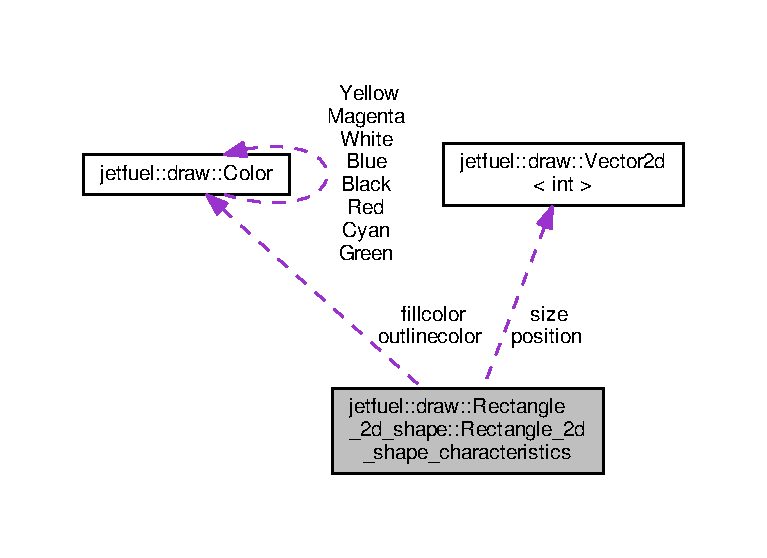
\includegraphics[width=350pt]{structjetfuel_1_1draw_1_1Rectangle__2d__shape_1_1Rectangle__2d__shape__characteristics__coll__graph}
\end{center}
\end{figure}
\subsection*{Public Attributes}
\begin{DoxyCompactItemize}
\item 
\mbox{\Hypertarget{structjetfuel_1_1draw_1_1Rectangle__2d__shape_1_1Rectangle__2d__shape__characteristics_afc9362283c71182811e3ed1b4a3b14ee}\label{structjetfuel_1_1draw_1_1Rectangle__2d__shape_1_1Rectangle__2d__shape__characteristics_afc9362283c71182811e3ed1b4a3b14ee}} 
\hyperlink{classjetfuel_1_1draw_1_1Vector2d}{Vector2d\+\_\+int} {\bfseries position}
\item 
\mbox{\Hypertarget{structjetfuel_1_1draw_1_1Rectangle__2d__shape_1_1Rectangle__2d__shape__characteristics_acddc8d54e69ac0583384aad76062d342}\label{structjetfuel_1_1draw_1_1Rectangle__2d__shape_1_1Rectangle__2d__shape__characteristics_acddc8d54e69ac0583384aad76062d342}} 
\hyperlink{classjetfuel_1_1draw_1_1Vector2d}{Vector2d\+\_\+int} {\bfseries size}
\item 
\mbox{\Hypertarget{structjetfuel_1_1draw_1_1Rectangle__2d__shape_1_1Rectangle__2d__shape__characteristics_a5774c2d3c7f2a470f2e0a4952e9ff8a8}\label{structjetfuel_1_1draw_1_1Rectangle__2d__shape_1_1Rectangle__2d__shape__characteristics_a5774c2d3c7f2a470f2e0a4952e9ff8a8}} 
\hyperlink{classjetfuel_1_1draw_1_1Color}{Color} {\bfseries fillcolor}
\item 
\mbox{\Hypertarget{structjetfuel_1_1draw_1_1Rectangle__2d__shape_1_1Rectangle__2d__shape__characteristics_adb7f45cc00b5e1f96c248b4d6fa592f4}\label{structjetfuel_1_1draw_1_1Rectangle__2d__shape_1_1Rectangle__2d__shape__characteristics_adb7f45cc00b5e1f96c248b4d6fa592f4}} 
\hyperlink{classjetfuel_1_1draw_1_1Color}{Color} {\bfseries outlinecolor}
\end{DoxyCompactItemize}


The documentation for this struct was generated from the following file\+:\begin{DoxyCompactItemize}
\item 
include/jetfueldraw/rectangle2dshape.\+h\end{DoxyCompactItemize}

\hypertarget{classjetfuel_1_1draw_1_1Rectangle__interface}{}\section{jetfuel\+:\+:draw\+:\+:Rectangle\+\_\+interface Class Reference}
\label{classjetfuel_1_1draw_1_1Rectangle__interface}\index{jetfuel\+::draw\+::\+Rectangle\+\_\+interface@{jetfuel\+::draw\+::\+Rectangle\+\_\+interface}}


{\ttfamily \#include $<$rectangleinterface.\+h$>$}



Inheritance diagram for jetfuel\+:\+:draw\+:\+:Rectangle\+\_\+interface\+:\nopagebreak
\begin{figure}[H]
\begin{center}
\leavevmode
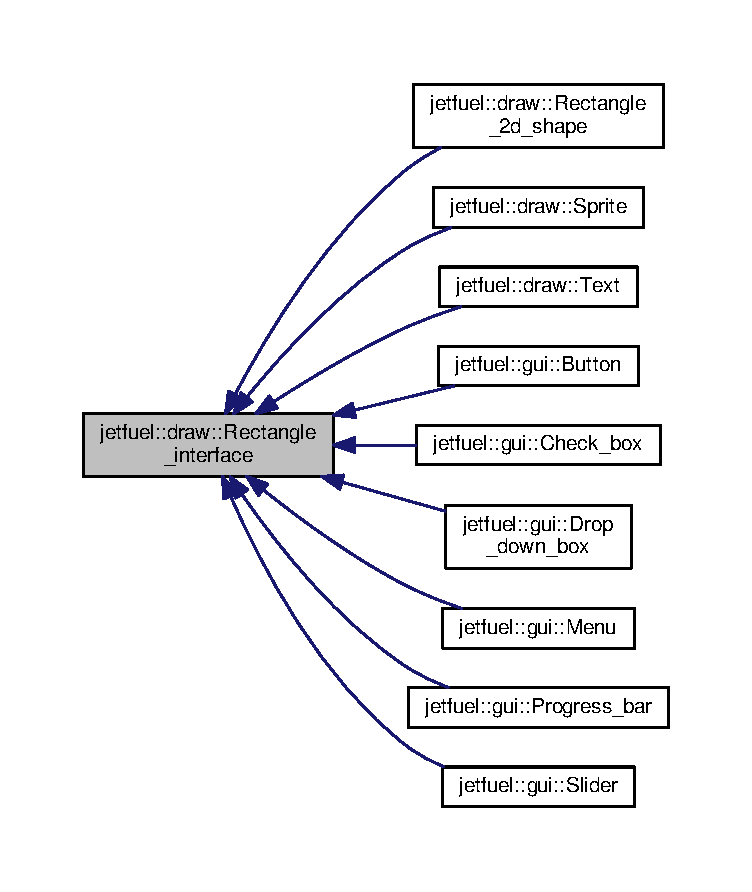
\includegraphics[width=350pt]{classjetfuel_1_1draw_1_1Rectangle__interface__inherit__graph}
\end{center}
\end{figure}
\subsection*{Public Member Functions}
\begin{DoxyCompactItemize}
\item 
virtual \hyperlink{classjetfuel_1_1draw_1_1Rect2d}{Rect2d\+\_\+int} \hyperlink{classjetfuel_1_1draw_1_1Rectangle__interface_a03fd3b6842ab7b3065379caec407296f}{Get\+\_\+rect\+\_\+to\+\_\+draw} ()=0
\begin{DoxyCompactList}\small\item\em Returns the \hyperlink{classjetfuel_1_1draw_1_1Rect2d}{Rect2d} to be drawn. \end{DoxyCompactList}\end{DoxyCompactItemize}


\subsection{Detailed Description}
A simple interface that specifies unique functions \hyperlink{classjetfuel_1_1draw_1_1Drawable}{Drawable} rectangles should implement.

\begin{DoxySeeAlso}{See also}
\hyperlink{classjetfuel_1_1draw_1_1Sprite}{jetfuel\+::draw\+::\+Sprite} 

\hyperlink{classjetfuel_1_1draw_1_1Rectangle__2d__shape}{jetfuel\+::draw\+::\+Rectangle\+\_\+2d\+\_\+shape} 

\hyperlink{classjetfuel_1_1draw_1_1Text}{jetfuel\+::draw\+::\+Text} 
\end{DoxySeeAlso}


\subsection{Member Function Documentation}
\mbox{\Hypertarget{classjetfuel_1_1draw_1_1Rectangle__interface_a03fd3b6842ab7b3065379caec407296f}\label{classjetfuel_1_1draw_1_1Rectangle__interface_a03fd3b6842ab7b3065379caec407296f}} 
\index{jetfuel\+::draw\+::\+Rectangle\+\_\+interface@{jetfuel\+::draw\+::\+Rectangle\+\_\+interface}!Get\+\_\+rect\+\_\+to\+\_\+draw@{Get\+\_\+rect\+\_\+to\+\_\+draw}}
\index{Get\+\_\+rect\+\_\+to\+\_\+draw@{Get\+\_\+rect\+\_\+to\+\_\+draw}!jetfuel\+::draw\+::\+Rectangle\+\_\+interface@{jetfuel\+::draw\+::\+Rectangle\+\_\+interface}}
\subsubsection{\texorpdfstring{Get\+\_\+rect\+\_\+to\+\_\+draw()}{Get\_rect\_to\_draw()}}
{\footnotesize\ttfamily virtual \hyperlink{classjetfuel_1_1draw_1_1Rect2d}{Rect2d\+\_\+int} jetfuel\+::draw\+::\+Rectangle\+\_\+interface\+::\+Get\+\_\+rect\+\_\+to\+\_\+draw (\begin{DoxyParamCaption}{ }\end{DoxyParamCaption})\hspace{0.3cm}{\ttfamily [pure virtual]}}



Returns the \hyperlink{classjetfuel_1_1draw_1_1Rect2d}{Rect2d} to be drawn. 

Returns the \hyperlink{classjetfuel_1_1draw_1_1Rect2d}{jetfuel\+::draw\+::\+Rect2d} to be drawn when Draw() is called. This is a pure virtual function that must be implemented by the children. This Rect2d\+\_\+int will be a rectangle of the entire \hyperlink{classjetfuel_1_1draw_1_1Drawable}{Drawable}. 

Implemented in \hyperlink{classjetfuel_1_1draw_1_1Text_a362996e996d471729944eebdff1f7636}{jetfuel\+::draw\+::\+Text}, \hyperlink{classjetfuel_1_1gui_1_1Menu_a1d5c050dcad48008898eafe2d610eff6}{jetfuel\+::gui\+::\+Menu}, \hyperlink{classjetfuel_1_1gui_1_1Button_a99615af8c169d2274b1593a29fdaf7ca}{jetfuel\+::gui\+::\+Button}, \hyperlink{classjetfuel_1_1gui_1_1Check__box_a09feae5781a788df462be6276e2d1c54}{jetfuel\+::gui\+::\+Check\+\_\+box}, \hyperlink{classjetfuel_1_1gui_1_1Drop__down__box_ab07ac526f3c2e9930398d78c7cad2d52}{jetfuel\+::gui\+::\+Drop\+\_\+down\+\_\+box}, \hyperlink{classjetfuel_1_1gui_1_1Slider_abab31dbe01b716b4e82919f0d8aba96c}{jetfuel\+::gui\+::\+Slider}, \hyperlink{classjetfuel_1_1gui_1_1Progress__bar_a4a09c3d515c9754b8295a4b5d83291ff}{jetfuel\+::gui\+::\+Progress\+\_\+bar}, \hyperlink{classjetfuel_1_1draw_1_1Rectangle__2d__shape_a1ed2975565e629d2b8d3fffa0a4756b2}{jetfuel\+::draw\+::\+Rectangle\+\_\+2d\+\_\+shape}, and \hyperlink{classjetfuel_1_1draw_1_1Sprite_a2cd3f83c4fc573be82d3dc3a9c70e317}{jetfuel\+::draw\+::\+Sprite}.



The documentation for this class was generated from the following file\+:\begin{DoxyCompactItemize}
\item 
include/jetfueldraw/rectangleinterface.\+h\end{DoxyCompactItemize}

\hypertarget{classjetfuel_1_1draw_1_1Scene}{}\section{jetfuel\+:\+:draw\+:\+:Scene Class Reference}
\label{classjetfuel_1_1draw_1_1Scene}\index{jetfuel\+::draw\+::\+Scene@{jetfuel\+::draw\+::\+Scene}}


{\ttfamily \#include $<$scene.\+h$>$}

\subsection*{Public Member Functions}
\begin{DoxyCompactItemize}
\item 
\hyperlink{classjetfuel_1_1draw_1_1Scene_ad27192ba7e5f0cb23b55f5ba067cbe94}{Scene} (const int id=0, const std\+::string label=\char`\"{}\char`\"{})
\begin{DoxyCompactList}\small\item\em Constructs a \hyperlink{classjetfuel_1_1draw_1_1Scene}{Scene} with a \hyperlink{classjetfuel_1_1draw_1_1Scene}{Scene} id. \end{DoxyCompactList}\item 
virtual \hyperlink{classjetfuel_1_1draw_1_1Scene_ac3e990c0deba1b5bb8d0552033a4ad81}{$\sim$\+Scene} ()
\begin{DoxyCompactList}\small\item\em Cleans up \hyperlink{classjetfuel_1_1draw_1_1Scene}{Scene} objects. \end{DoxyCompactList}\item 
bool \hyperlink{classjetfuel_1_1draw_1_1Scene_aea4b4c4ae25c30d661be4c52787e0ea3}{Attach\+\_\+drawable} (\hyperlink{classjetfuel_1_1draw_1_1Drawable}{Drawable} $\ast$drawable, const unsigned int drawingweight)
\begin{DoxyCompactList}\small\item\em Attaches a \hyperlink{classjetfuel_1_1draw_1_1Drawable}{Drawable} to the \hyperlink{classjetfuel_1_1draw_1_1Scene}{Scene}. \end{DoxyCompactList}\item 
void \hyperlink{classjetfuel_1_1draw_1_1Scene_ab7bf5496c18d4a00e0b5ce02a203a4b4}{Disable\+\_\+drawable} (\hyperlink{classjetfuel_1_1draw_1_1Drawable}{Drawable} $\ast$drawable)
\begin{DoxyCompactList}\small\item\em Disables a \hyperlink{classjetfuel_1_1draw_1_1Drawable}{Drawable} already attached to the \hyperlink{classjetfuel_1_1draw_1_1Scene}{Scene}. \end{DoxyCompactList}\item 
\mbox{\Hypertarget{classjetfuel_1_1draw_1_1Scene_ab84abd926680576fe264a23d732307e8}\label{classjetfuel_1_1draw_1_1Scene_ab84abd926680576fe264a23d732307e8}} 
void {\bfseries Enable\+\_\+drawable} (\hyperlink{classjetfuel_1_1draw_1_1Drawable}{Drawable} $\ast$drawable)
\item 
int \hyperlink{classjetfuel_1_1draw_1_1Scene_a03433414bcb71d2001ecc717800b628b}{Get\+\_\+scene\+\_\+id} () const
\begin{DoxyCompactList}\small\item\em Returns the \hyperlink{classjetfuel_1_1draw_1_1Scene}{Scene}\textquotesingle{}s id. \end{DoxyCompactList}\item 
\hyperlink{classjetfuel_1_1draw_1_1Color}{Color} \hyperlink{classjetfuel_1_1draw_1_1Scene_a212ff5b6cb07e2332b92ef72f5d67819}{Get\+\_\+background\+\_\+color} () const
\begin{DoxyCompactList}\small\item\em Gets the scene\textquotesingle{}s background color. \end{DoxyCompactList}\item 
void \hyperlink{classjetfuel_1_1draw_1_1Scene_aa3d099d358cd8ad9274d633805f3cc43}{Set\+\_\+background\+\_\+color} (const \hyperlink{classjetfuel_1_1draw_1_1Color}{Color} backgroundcolor)
\begin{DoxyCompactList}\small\item\em Sets the background color of the \hyperlink{classjetfuel_1_1draw_1_1Scene}{Scene}. \end{DoxyCompactList}\item 
void \hyperlink{classjetfuel_1_1draw_1_1Scene_a6ee0359540800521294fda5d1d8b86b1}{Reset\+\_\+scene} ()
\begin{DoxyCompactList}\small\item\em Clears the \hyperlink{classjetfuel_1_1draw_1_1Scene}{Scene} of any previously attached objects. \end{DoxyCompactList}\item 
void \hyperlink{classjetfuel_1_1draw_1_1Scene_a0cd111e8863ab2e9e78cd3b6144c64a8}{Assign\+\_\+renderer} (S\+D\+L\+\_\+\+Renderer $\ast$scenemanagerrenderer)
\begin{DoxyCompactList}\small\item\em Assigns a renderer to use when rendering a \hyperlink{classjetfuel_1_1draw_1_1Sprite}{Sprite}. \end{DoxyCompactList}\item 
void \hyperlink{classjetfuel_1_1draw_1_1Scene_a80b9b5f38022b6c2af9921656f93056b}{Draw\+\_\+scene} ()
\begin{DoxyCompactList}\small\item\em Draws the \hyperlink{classjetfuel_1_1draw_1_1Scene}{Scene}. \end{DoxyCompactList}\end{DoxyCompactItemize}
\subsection*{Protected Member Functions}
\begin{DoxyCompactItemize}
\item 
S\+D\+L\+\_\+\+Renderer $\ast$ \hyperlink{classjetfuel_1_1draw_1_1Scene_abb0c1a20e3bb87167c75ada894acd60b}{Get\+\_\+scene\+\_\+manager\+\_\+renderer} () const
\begin{DoxyCompactList}\small\item\em Returns the scene manager\textquotesingle{}s renderer. \end{DoxyCompactList}\item 
size\+\_\+t \hyperlink{classjetfuel_1_1draw_1_1Scene_a62423470cca53acd55ff174d6e37d730}{Get\+\_\+size\+\_\+of\+\_\+drawables\+\_\+vector} () const
\begin{DoxyCompactList}\small\item\em Returns the size of the internal m\+\_\+drawables vector. \end{DoxyCompactList}\item 
\hyperlink{classjetfuel_1_1draw_1_1Drawable}{Drawable} $\ast$ \hyperlink{classjetfuel_1_1draw_1_1Scene_ad22707818e9de20b28d82646ca460141}{Get\+\_\+drawable\+\_\+in\+\_\+vector} (size\+\_\+t place)
\begin{DoxyCompactList}\small\item\em Returns a \hyperlink{classjetfuel_1_1draw_1_1Drawable}{Drawable}\textquotesingle{}s reference in the internal m\+\_\+drawables vector. \end{DoxyCompactList}\item 
unsigned int \hyperlink{classjetfuel_1_1draw_1_1Scene_a92228a8f31c8e2e1fe1e3d0a12940b1a}{Get\+\_\+drawable\+\_\+placement\+\_\+in\+\_\+vector} (size\+\_\+t place)
\begin{DoxyCompactList}\small\item\em Gets \hyperlink{classjetfuel_1_1draw_1_1Drawable}{Drawable}\textquotesingle{}s placement (or drawingweight) in vector. \end{DoxyCompactList}\item 
void \hyperlink{classjetfuel_1_1draw_1_1Scene_a4ab618141cf7e10c95cbe7b114688c1a}{Add\+\_\+drawable\+\_\+placement\+\_\+to\+\_\+drawable\+\_\+placement\+\_\+vector} (const unsigned int placement)
\begin{DoxyCompactList}\small\item\em Adds a \hyperlink{classjetfuel_1_1draw_1_1Drawable}{Drawable} placement (or drawingweight) to the \hyperlink{classjetfuel_1_1draw_1_1Drawable}{Drawable} placement vector. \end{DoxyCompactList}\item 
unsigned int \hyperlink{classjetfuel_1_1draw_1_1Scene_a439de5e14d13f06db5acd2da708dc177}{Get\+\_\+highest\+\_\+placement} () const
\begin{DoxyCompactList}\small\item\em Gets the highest \hyperlink{classjetfuel_1_1draw_1_1Drawable}{Drawable} placement (or drawingweight) of the \hyperlink{classjetfuel_1_1draw_1_1Drawable}{Drawable} placement vector. \end{DoxyCompactList}\item 
void \hyperlink{classjetfuel_1_1draw_1_1Scene_a58984e589bd7ffa2940299fa88388765}{Add\+\_\+drawable\+\_\+to\+\_\+drawable\+\_\+vector} (\hyperlink{classjetfuel_1_1draw_1_1Drawable}{Drawable} $\ast$drawable)
\begin{DoxyCompactList}\small\item\em Adds a drawable to the scene. \end{DoxyCompactList}\item 
bool \hyperlink{classjetfuel_1_1draw_1_1Scene_a7442f49028075ad2da9d3c2e450fbe4d}{Get\+\_\+drawable\+\_\+status} (size\+\_\+t place) const
\begin{DoxyCompactList}\small\item\em Gets a \hyperlink{classjetfuel_1_1draw_1_1Drawable}{Drawable}\textquotesingle{}s status in the drawablesenabled vector. \end{DoxyCompactList}\item 
void \hyperlink{classjetfuel_1_1draw_1_1Scene_a517687bb7b400a9e0b82c4c53e1939cc}{Enable\+\_\+drawable\+\_\+in\+\_\+vector} (size\+\_\+t place)
\begin{DoxyCompactList}\small\item\em Enables a \hyperlink{classjetfuel_1_1draw_1_1Drawable}{Drawable} to be drawn when Draw\+\_\+scene is called. \end{DoxyCompactList}\item 
void \hyperlink{classjetfuel_1_1draw_1_1Scene_a725618dfecbdb201fba44be02cc2bc13}{Disable\+\_\+drawable\+\_\+in\+\_\+vector} (size\+\_\+t place)
\begin{DoxyCompactList}\small\item\em Disables a \hyperlink{classjetfuel_1_1draw_1_1Drawable}{Drawable} to not be drawn when Draw\+\_\+scene is called. \end{DoxyCompactList}\item 
bool \hyperlink{classjetfuel_1_1draw_1_1Scene_a1d8d53f33a18643e5ee7ea05e9906786}{Is\+\_\+background\+\_\+color\+\_\+set} () const
\begin{DoxyCompactList}\small\item\em Checks whether the \hyperlink{classjetfuel_1_1draw_1_1Scene}{Scene}\textquotesingle{}s background color is set. \end{DoxyCompactList}\end{DoxyCompactItemize}


\subsection{Detailed Description}
A scene to be used with \hyperlink{classjetfuel_1_1draw_1_1Scene__manager}{Scene\+\_\+manager} to produce a series of drawable scenes to be presented to the player.

Code Example\+: \hyperlink{classjetfuel_1_1draw_1_1Scene__manager}{jetfuel\+::draw\+::\+Scene\+\_\+manager} scenemanager; \hyperlink{classjetfuel_1_1draw_1_1Scene}{jetfuel\+::draw\+::\+Scene} scene1(1); \hyperlink{classjetfuel_1_1draw_1_1Image}{jetfuel\+::draw\+::\+Image} image = \hyperlink{classjetfuel_1_1draw_1_1Image}{jetfuel\+::draw\+::\+Image}(\char`\"{}test.\+png\char`\"{}); \hyperlink{classjetfuel_1_1draw_1_1Sprite}{jetfuel\+::draw\+::\+Sprite} background;

if(!scenemanager.Create\+\_\+window(\char`\"{}example\char`\"{}, jetfuel\+::draw\+::\+Vector2d\+\_\+int(0,0), jetfuel\+::draw\+::\+Vector2d\+\_\+int(500,500)))\{ std\+::cerr $<$$<$ \char`\"{}\mbox{[}!\mbox{]}\+E\+R\+R\+O\+R with creating sdl renderer!\char`\"{} $<$$<$ \char`\"{}\+Error is\+:\char`\"{} $<$$<$ S\+D\+L\+\_\+\+Get\+Error() $<$$<$ \char`\"{}\textbackslash{}n\char`\"{}; \}

if(!scenemanager.Create\+\_\+renderer())\{ std\+::cerr $<$$<$ \char`\"{}\mbox{[}!\mbox{]}\+E\+R\+R\+O\+R with creating sdl renderer!\char`\"{} $<$$<$ \char`\"{}\+Error is\+:\char`\"{} $<$$<$ S\+D\+L\+\_\+\+Get\+Error() $<$$<$ \char`\"{}\textbackslash{}n\char`\"{}; \}

scenemanager.\+Switch\+\_\+current\+\_\+scene(\&scene1); scene1.\+Attach\+\_\+drawable(\&background);

if(!background.Load\+\_\+from\+\_\+image(backgroundimage))\{ std\+::cerr $<$$<$ \char`\"{}\mbox{[}!\mbox{]}\+E\+R\+R\+O\+R with loading from image! Error is\+:\char`\"{} $<$$<$ I\+M\+G\+\_\+\+Get\+Error() $<$$<$ \char`\"{}\textbackslash{}n\char`\"{}; return 1; \}

background.\+Set\+\_\+position(jetfuel\+::draw\+::\+Vector2d\+\_\+int(0,0));

scenemanager.\+Draw\+\_\+current\+\_\+scene(); 

\subsection{Constructor \& Destructor Documentation}
\mbox{\Hypertarget{classjetfuel_1_1draw_1_1Scene_ad27192ba7e5f0cb23b55f5ba067cbe94}\label{classjetfuel_1_1draw_1_1Scene_ad27192ba7e5f0cb23b55f5ba067cbe94}} 
\index{jetfuel\+::draw\+::\+Scene@{jetfuel\+::draw\+::\+Scene}!Scene@{Scene}}
\index{Scene@{Scene}!jetfuel\+::draw\+::\+Scene@{jetfuel\+::draw\+::\+Scene}}
\subsubsection{\texorpdfstring{Scene()}{Scene()}}
{\footnotesize\ttfamily jetfuel\+::draw\+::\+Scene\+::\+Scene (\begin{DoxyParamCaption}\item[{const int}]{id = {\ttfamily 0},  }\item[{const std\+::string}]{label = {\ttfamily \char`\"{}\char`\"{}} }\end{DoxyParamCaption})}



Constructs a \hyperlink{classjetfuel_1_1draw_1_1Scene}{Scene} with a \hyperlink{classjetfuel_1_1draw_1_1Scene}{Scene} id. 

Constructs a \hyperlink{classjetfuel_1_1draw_1_1Scene}{Scene} with an optional \hyperlink{classjetfuel_1_1draw_1_1Scene}{Scene} id and label for categorization.


\begin{DoxyParams}{Parameters}
{\em int} & id \\
\hline
\end{DoxyParams}
\mbox{\Hypertarget{classjetfuel_1_1draw_1_1Scene_ac3e990c0deba1b5bb8d0552033a4ad81}\label{classjetfuel_1_1draw_1_1Scene_ac3e990c0deba1b5bb8d0552033a4ad81}} 
\index{jetfuel\+::draw\+::\+Scene@{jetfuel\+::draw\+::\+Scene}!````~Scene@{$\sim$\+Scene}}
\index{````~Scene@{$\sim$\+Scene}!jetfuel\+::draw\+::\+Scene@{jetfuel\+::draw\+::\+Scene}}
\subsubsection{\texorpdfstring{$\sim$\+Scene()}{~Scene()}}
{\footnotesize\ttfamily virtual jetfuel\+::draw\+::\+Scene\+::$\sim$\+Scene (\begin{DoxyParamCaption}{ }\end{DoxyParamCaption})\hspace{0.3cm}{\ttfamily [virtual]}}



Cleans up \hyperlink{classjetfuel_1_1draw_1_1Scene}{Scene} objects. 

Cleans up \hyperlink{classjetfuel_1_1draw_1_1Scene}{Scene} objects. 

\subsection{Member Function Documentation}
\mbox{\Hypertarget{classjetfuel_1_1draw_1_1Scene_a4ab618141cf7e10c95cbe7b114688c1a}\label{classjetfuel_1_1draw_1_1Scene_a4ab618141cf7e10c95cbe7b114688c1a}} 
\index{jetfuel\+::draw\+::\+Scene@{jetfuel\+::draw\+::\+Scene}!Add\+\_\+drawable\+\_\+placement\+\_\+to\+\_\+drawable\+\_\+placement\+\_\+vector@{Add\+\_\+drawable\+\_\+placement\+\_\+to\+\_\+drawable\+\_\+placement\+\_\+vector}}
\index{Add\+\_\+drawable\+\_\+placement\+\_\+to\+\_\+drawable\+\_\+placement\+\_\+vector@{Add\+\_\+drawable\+\_\+placement\+\_\+to\+\_\+drawable\+\_\+placement\+\_\+vector}!jetfuel\+::draw\+::\+Scene@{jetfuel\+::draw\+::\+Scene}}
\subsubsection{\texorpdfstring{Add\+\_\+drawable\+\_\+placement\+\_\+to\+\_\+drawable\+\_\+placement\+\_\+vector()}{Add\_drawable\_placement\_to\_drawable\_placement\_vector()}}
{\footnotesize\ttfamily void jetfuel\+::draw\+::\+Scene\+::\+Add\+\_\+drawable\+\_\+placement\+\_\+to\+\_\+drawable\+\_\+placement\+\_\+vector (\begin{DoxyParamCaption}\item[{const unsigned int}]{placement }\end{DoxyParamCaption})\hspace{0.3cm}{\ttfamily [inline]}, {\ttfamily [protected]}}



Adds a \hyperlink{classjetfuel_1_1draw_1_1Drawable}{Drawable} placement (or drawingweight) to the \hyperlink{classjetfuel_1_1draw_1_1Drawable}{Drawable} placement vector. 

Adds a \hyperlink{classjetfuel_1_1draw_1_1Drawable}{Drawable} placement (or drawingweight) to the \hyperlink{classjetfuel_1_1draw_1_1Drawable}{Drawable} placement vector.


\begin{DoxyParams}{Parameters}
{\em unsigned} & int placement \\
\hline
\end{DoxyParams}
\mbox{\Hypertarget{classjetfuel_1_1draw_1_1Scene_a58984e589bd7ffa2940299fa88388765}\label{classjetfuel_1_1draw_1_1Scene_a58984e589bd7ffa2940299fa88388765}} 
\index{jetfuel\+::draw\+::\+Scene@{jetfuel\+::draw\+::\+Scene}!Add\+\_\+drawable\+\_\+to\+\_\+drawable\+\_\+vector@{Add\+\_\+drawable\+\_\+to\+\_\+drawable\+\_\+vector}}
\index{Add\+\_\+drawable\+\_\+to\+\_\+drawable\+\_\+vector@{Add\+\_\+drawable\+\_\+to\+\_\+drawable\+\_\+vector}!jetfuel\+::draw\+::\+Scene@{jetfuel\+::draw\+::\+Scene}}
\subsubsection{\texorpdfstring{Add\+\_\+drawable\+\_\+to\+\_\+drawable\+\_\+vector()}{Add\_drawable\_to\_drawable\_vector()}}
{\footnotesize\ttfamily void jetfuel\+::draw\+::\+Scene\+::\+Add\+\_\+drawable\+\_\+to\+\_\+drawable\+\_\+vector (\begin{DoxyParamCaption}\item[{\hyperlink{classjetfuel_1_1draw_1_1Drawable}{Drawable} $\ast$}]{drawable }\end{DoxyParamCaption})\hspace{0.3cm}{\ttfamily [inline]}, {\ttfamily [protected]}}



Adds a drawable to the scene. 

Adds a drawable to the scene to be drawn upon the the function \hyperlink{classjetfuel_1_1draw_1_1Scene_a80b9b5f38022b6c2af9921656f93056b}{Draw\+\_\+scene()} being called.


\begin{DoxyParams}{Parameters}
{\em \hyperlink{classjetfuel_1_1draw_1_1Drawable}{Drawable}} & $\ast$drawable \\
\hline
\end{DoxyParams}
\mbox{\Hypertarget{classjetfuel_1_1draw_1_1Scene_a0cd111e8863ab2e9e78cd3b6144c64a8}\label{classjetfuel_1_1draw_1_1Scene_a0cd111e8863ab2e9e78cd3b6144c64a8}} 
\index{jetfuel\+::draw\+::\+Scene@{jetfuel\+::draw\+::\+Scene}!Assign\+\_\+renderer@{Assign\+\_\+renderer}}
\index{Assign\+\_\+renderer@{Assign\+\_\+renderer}!jetfuel\+::draw\+::\+Scene@{jetfuel\+::draw\+::\+Scene}}
\subsubsection{\texorpdfstring{Assign\+\_\+renderer()}{Assign\_renderer()}}
{\footnotesize\ttfamily void jetfuel\+::draw\+::\+Scene\+::\+Assign\+\_\+renderer (\begin{DoxyParamCaption}\item[{S\+D\+L\+\_\+\+Renderer $\ast$}]{scenemanagerrenderer }\end{DoxyParamCaption})\hspace{0.3cm}{\ttfamily [inline]}}



Assigns a renderer to use when rendering a \hyperlink{classjetfuel_1_1draw_1_1Sprite}{Sprite}. 

Assigns a renderer to use when rendering a \hyperlink{classjetfuel_1_1draw_1_1Drawable}{Drawable}. This function should be called by a \hyperlink{classjetfuel_1_1draw_1_1Scene__manager}{Scene\+\_\+manager} upon switching scenes.


\begin{DoxyParams}{Parameters}
{\em S\+D\+L\+\_\+\+Renderer} & $\ast$scenemanagerrenderer \\
\hline
\end{DoxyParams}
\mbox{\Hypertarget{classjetfuel_1_1draw_1_1Scene_aea4b4c4ae25c30d661be4c52787e0ea3}\label{classjetfuel_1_1draw_1_1Scene_aea4b4c4ae25c30d661be4c52787e0ea3}} 
\index{jetfuel\+::draw\+::\+Scene@{jetfuel\+::draw\+::\+Scene}!Attach\+\_\+drawable@{Attach\+\_\+drawable}}
\index{Attach\+\_\+drawable@{Attach\+\_\+drawable}!jetfuel\+::draw\+::\+Scene@{jetfuel\+::draw\+::\+Scene}}
\subsubsection{\texorpdfstring{Attach\+\_\+drawable()}{Attach\_drawable()}}
{\footnotesize\ttfamily bool jetfuel\+::draw\+::\+Scene\+::\+Attach\+\_\+drawable (\begin{DoxyParamCaption}\item[{\hyperlink{classjetfuel_1_1draw_1_1Drawable}{Drawable} $\ast$}]{drawable,  }\item[{const unsigned int}]{drawingweight }\end{DoxyParamCaption})}



Attaches a \hyperlink{classjetfuel_1_1draw_1_1Drawable}{Drawable} to the \hyperlink{classjetfuel_1_1draw_1_1Scene}{Scene}. 

Attaches a \hyperlink{classjetfuel_1_1draw_1_1Drawable}{Drawable}\textquotesingle{}s reference and a drawingweight to the \hyperlink{classjetfuel_1_1draw_1_1Scene}{Scene} to be drawn upon the function \hyperlink{classjetfuel_1_1draw_1_1Scene_a80b9b5f38022b6c2af9921656f93056b}{Draw\+\_\+scene()} being called. Lower drawingweights are drawn lower, and might overlap with another higher weighted \hyperlink{classjetfuel_1_1draw_1_1Drawable}{Drawable}. Sprites on the same drawingweight will be overlapped by Rectangle\+\_\+2d\+\_\+shapes and Texts.


\begin{DoxyParams}{Parameters}
{\em \hyperlink{classjetfuel_1_1draw_1_1Drawable}{Drawable}} & $\ast$drawable \\
\hline
{\em unsigned} & int drawingweight \\
\hline
\end{DoxyParams}
\mbox{\Hypertarget{classjetfuel_1_1draw_1_1Scene_ab7bf5496c18d4a00e0b5ce02a203a4b4}\label{classjetfuel_1_1draw_1_1Scene_ab7bf5496c18d4a00e0b5ce02a203a4b4}} 
\index{jetfuel\+::draw\+::\+Scene@{jetfuel\+::draw\+::\+Scene}!Disable\+\_\+drawable@{Disable\+\_\+drawable}}
\index{Disable\+\_\+drawable@{Disable\+\_\+drawable}!jetfuel\+::draw\+::\+Scene@{jetfuel\+::draw\+::\+Scene}}
\subsubsection{\texorpdfstring{Disable\+\_\+drawable()}{Disable\_drawable()}}
{\footnotesize\ttfamily void jetfuel\+::draw\+::\+Scene\+::\+Disable\+\_\+drawable (\begin{DoxyParamCaption}\item[{\hyperlink{classjetfuel_1_1draw_1_1Drawable}{Drawable} $\ast$}]{drawable }\end{DoxyParamCaption})}



Disables a \hyperlink{classjetfuel_1_1draw_1_1Drawable}{Drawable} already attached to the \hyperlink{classjetfuel_1_1draw_1_1Scene}{Scene}. 

Disables a \hyperlink{classjetfuel_1_1draw_1_1Drawable}{Drawable} already attached to the \hyperlink{classjetfuel_1_1draw_1_1Scene}{Scene}. This associates that \hyperlink{classjetfuel_1_1draw_1_1Drawable}{Drawable} with a bool of false in a \hyperlink{classjetfuel_1_1draw_1_1Drawable}{Drawable} status vector, which dictates whenever a certain \hyperlink{classjetfuel_1_1draw_1_1Drawable}{Drawable} should be drawed. This allows you to re-\/enable this \hyperlink{classjetfuel_1_1draw_1_1Drawable}{Drawable} any time by calling the Enable\+\_\+drawable function. If the drawable passed in is not found in this \hyperlink{classjetfuel_1_1draw_1_1Scene}{Scene} object, this function will not do anything


\begin{DoxyParams}{Parameters}
{\em \hyperlink{classjetfuel_1_1draw_1_1Drawable}{Drawable}} & $\ast$drawable \\
\hline
\end{DoxyParams}
\mbox{\Hypertarget{classjetfuel_1_1draw_1_1Scene_a725618dfecbdb201fba44be02cc2bc13}\label{classjetfuel_1_1draw_1_1Scene_a725618dfecbdb201fba44be02cc2bc13}} 
\index{jetfuel\+::draw\+::\+Scene@{jetfuel\+::draw\+::\+Scene}!Disable\+\_\+drawable\+\_\+in\+\_\+vector@{Disable\+\_\+drawable\+\_\+in\+\_\+vector}}
\index{Disable\+\_\+drawable\+\_\+in\+\_\+vector@{Disable\+\_\+drawable\+\_\+in\+\_\+vector}!jetfuel\+::draw\+::\+Scene@{jetfuel\+::draw\+::\+Scene}}
\subsubsection{\texorpdfstring{Disable\+\_\+drawable\+\_\+in\+\_\+vector()}{Disable\_drawable\_in\_vector()}}
{\footnotesize\ttfamily void jetfuel\+::draw\+::\+Scene\+::\+Disable\+\_\+drawable\+\_\+in\+\_\+vector (\begin{DoxyParamCaption}\item[{size\+\_\+t}]{place }\end{DoxyParamCaption})\hspace{0.3cm}{\ttfamily [inline]}, {\ttfamily [protected]}}



Disables a \hyperlink{classjetfuel_1_1draw_1_1Drawable}{Drawable} to not be drawn when Draw\+\_\+scene is called. 

Disables a \hyperlink{classjetfuel_1_1draw_1_1Drawable}{Drawable} to not be drawn when Draw\+\_\+scene is called.


\begin{DoxyParams}{Parameters}
{\em size\+\_\+t} & place \\
\hline
\end{DoxyParams}
\mbox{\Hypertarget{classjetfuel_1_1draw_1_1Scene_a80b9b5f38022b6c2af9921656f93056b}\label{classjetfuel_1_1draw_1_1Scene_a80b9b5f38022b6c2af9921656f93056b}} 
\index{jetfuel\+::draw\+::\+Scene@{jetfuel\+::draw\+::\+Scene}!Draw\+\_\+scene@{Draw\+\_\+scene}}
\index{Draw\+\_\+scene@{Draw\+\_\+scene}!jetfuel\+::draw\+::\+Scene@{jetfuel\+::draw\+::\+Scene}}
\subsubsection{\texorpdfstring{Draw\+\_\+scene()}{Draw\_scene()}}
{\footnotesize\ttfamily void jetfuel\+::draw\+::\+Scene\+::\+Draw\+\_\+scene (\begin{DoxyParamCaption}{ }\end{DoxyParamCaption})}



Draws the \hyperlink{classjetfuel_1_1draw_1_1Scene}{Scene}. 

Draws the \hyperlink{classjetfuel_1_1draw_1_1Scene}{Scene} by drawing all of the attached drawable objects. This function should be called by a \hyperlink{classjetfuel_1_1draw_1_1Scene__manager}{jetfuel\+::draw\+::\+Scene\+\_\+manager} upon the function \hyperlink{classjetfuel_1_1draw_1_1Scene__manager_a8af9a3abfd5121b1b8556342de435773}{jetfuel\+::draw\+::\+Scene\+\_\+manager\+::\+Draw\+\_\+current\+\_\+scene()} being called. \mbox{\Hypertarget{classjetfuel_1_1draw_1_1Scene_a517687bb7b400a9e0b82c4c53e1939cc}\label{classjetfuel_1_1draw_1_1Scene_a517687bb7b400a9e0b82c4c53e1939cc}} 
\index{jetfuel\+::draw\+::\+Scene@{jetfuel\+::draw\+::\+Scene}!Enable\+\_\+drawable\+\_\+in\+\_\+vector@{Enable\+\_\+drawable\+\_\+in\+\_\+vector}}
\index{Enable\+\_\+drawable\+\_\+in\+\_\+vector@{Enable\+\_\+drawable\+\_\+in\+\_\+vector}!jetfuel\+::draw\+::\+Scene@{jetfuel\+::draw\+::\+Scene}}
\subsubsection{\texorpdfstring{Enable\+\_\+drawable\+\_\+in\+\_\+vector()}{Enable\_drawable\_in\_vector()}}
{\footnotesize\ttfamily void jetfuel\+::draw\+::\+Scene\+::\+Enable\+\_\+drawable\+\_\+in\+\_\+vector (\begin{DoxyParamCaption}\item[{size\+\_\+t}]{place }\end{DoxyParamCaption})\hspace{0.3cm}{\ttfamily [inline]}, {\ttfamily [protected]}}



Enables a \hyperlink{classjetfuel_1_1draw_1_1Drawable}{Drawable} to be drawn when Draw\+\_\+scene is called. 

Enables a \hyperlink{classjetfuel_1_1draw_1_1Drawable}{Drawable} to be drawn when Draw\+\_\+scene is called.


\begin{DoxyParams}{Parameters}
{\em size\+\_\+t} & place \\
\hline
\end{DoxyParams}
\mbox{\Hypertarget{classjetfuel_1_1draw_1_1Scene_a212ff5b6cb07e2332b92ef72f5d67819}\label{classjetfuel_1_1draw_1_1Scene_a212ff5b6cb07e2332b92ef72f5d67819}} 
\index{jetfuel\+::draw\+::\+Scene@{jetfuel\+::draw\+::\+Scene}!Get\+\_\+background\+\_\+color@{Get\+\_\+background\+\_\+color}}
\index{Get\+\_\+background\+\_\+color@{Get\+\_\+background\+\_\+color}!jetfuel\+::draw\+::\+Scene@{jetfuel\+::draw\+::\+Scene}}
\subsubsection{\texorpdfstring{Get\+\_\+background\+\_\+color()}{Get\_background\_color()}}
{\footnotesize\ttfamily \hyperlink{classjetfuel_1_1draw_1_1Color}{Color} jetfuel\+::draw\+::\+Scene\+::\+Get\+\_\+background\+\_\+color (\begin{DoxyParamCaption}{ }\end{DoxyParamCaption}) const\hspace{0.3cm}{\ttfamily [inline]}}



Gets the scene\textquotesingle{}s background color. 

Gets the scene\textquotesingle{}s background color. This color will be black by default if it has not been set. \mbox{\Hypertarget{classjetfuel_1_1draw_1_1Scene_ad22707818e9de20b28d82646ca460141}\label{classjetfuel_1_1draw_1_1Scene_ad22707818e9de20b28d82646ca460141}} 
\index{jetfuel\+::draw\+::\+Scene@{jetfuel\+::draw\+::\+Scene}!Get\+\_\+drawable\+\_\+in\+\_\+vector@{Get\+\_\+drawable\+\_\+in\+\_\+vector}}
\index{Get\+\_\+drawable\+\_\+in\+\_\+vector@{Get\+\_\+drawable\+\_\+in\+\_\+vector}!jetfuel\+::draw\+::\+Scene@{jetfuel\+::draw\+::\+Scene}}
\subsubsection{\texorpdfstring{Get\+\_\+drawable\+\_\+in\+\_\+vector()}{Get\_drawable\_in\_vector()}}
{\footnotesize\ttfamily \hyperlink{classjetfuel_1_1draw_1_1Drawable}{Drawable}$\ast$ jetfuel\+::draw\+::\+Scene\+::\+Get\+\_\+drawable\+\_\+in\+\_\+vector (\begin{DoxyParamCaption}\item[{size\+\_\+t}]{place }\end{DoxyParamCaption})\hspace{0.3cm}{\ttfamily [inline]}, {\ttfamily [protected]}}



Returns a \hyperlink{classjetfuel_1_1draw_1_1Drawable}{Drawable}\textquotesingle{}s reference in the internal m\+\_\+drawables vector. 

Returns a \hyperlink{classjetfuel_1_1draw_1_1Drawable}{Drawable}\textquotesingle{}s reference in the internal private m\+\_\+drawables vector. If place is not in the \hyperlink{classjetfuel_1_1draw_1_1Drawable}{Drawable}\textquotesingle{}s vector range, this function will throw a jetfuel\+::core\+::exceptions \+::\+Out\+\_\+of\+\_\+vector\+\_\+range\+\_\+exception(). Otherwise, it will return that \hyperlink{classjetfuel_1_1draw_1_1Drawable}{Drawable}\textquotesingle{}s reference.


\begin{DoxyParams}{Parameters}
{\em size\+\_\+t} & place \\
\hline
\end{DoxyParams}
\mbox{\Hypertarget{classjetfuel_1_1draw_1_1Scene_a92228a8f31c8e2e1fe1e3d0a12940b1a}\label{classjetfuel_1_1draw_1_1Scene_a92228a8f31c8e2e1fe1e3d0a12940b1a}} 
\index{jetfuel\+::draw\+::\+Scene@{jetfuel\+::draw\+::\+Scene}!Get\+\_\+drawable\+\_\+placement\+\_\+in\+\_\+vector@{Get\+\_\+drawable\+\_\+placement\+\_\+in\+\_\+vector}}
\index{Get\+\_\+drawable\+\_\+placement\+\_\+in\+\_\+vector@{Get\+\_\+drawable\+\_\+placement\+\_\+in\+\_\+vector}!jetfuel\+::draw\+::\+Scene@{jetfuel\+::draw\+::\+Scene}}
\subsubsection{\texorpdfstring{Get\+\_\+drawable\+\_\+placement\+\_\+in\+\_\+vector()}{Get\_drawable\_placement\_in\_vector()}}
{\footnotesize\ttfamily unsigned int jetfuel\+::draw\+::\+Scene\+::\+Get\+\_\+drawable\+\_\+placement\+\_\+in\+\_\+vector (\begin{DoxyParamCaption}\item[{size\+\_\+t}]{place }\end{DoxyParamCaption})\hspace{0.3cm}{\ttfamily [inline]}, {\ttfamily [protected]}}



Gets \hyperlink{classjetfuel_1_1draw_1_1Drawable}{Drawable}\textquotesingle{}s placement (or drawingweight) in vector. 

Gets \hyperlink{classjetfuel_1_1draw_1_1Drawable}{Drawable}\textquotesingle{}s placement (or drawingweight) in vector. If this function is given a place that is bigger or equal to the vector\textquotesingle{}s size, this function will throw a jetfuel\+::core\+::exceptions \+::\+Out\+\_\+of\+\_\+vector\+\_\+range\+\_\+exception() exception. Otherwise, this function will return that \hyperlink{classjetfuel_1_1draw_1_1Drawable}{Drawable}\textquotesingle{}s placement.


\begin{DoxyParams}{Parameters}
{\em size\+\_\+t} & place \\
\hline
\end{DoxyParams}
\mbox{\Hypertarget{classjetfuel_1_1draw_1_1Scene_a7442f49028075ad2da9d3c2e450fbe4d}\label{classjetfuel_1_1draw_1_1Scene_a7442f49028075ad2da9d3c2e450fbe4d}} 
\index{jetfuel\+::draw\+::\+Scene@{jetfuel\+::draw\+::\+Scene}!Get\+\_\+drawable\+\_\+status@{Get\+\_\+drawable\+\_\+status}}
\index{Get\+\_\+drawable\+\_\+status@{Get\+\_\+drawable\+\_\+status}!jetfuel\+::draw\+::\+Scene@{jetfuel\+::draw\+::\+Scene}}
\subsubsection{\texorpdfstring{Get\+\_\+drawable\+\_\+status()}{Get\_drawable\_status()}}
{\footnotesize\ttfamily bool jetfuel\+::draw\+::\+Scene\+::\+Get\+\_\+drawable\+\_\+status (\begin{DoxyParamCaption}\item[{size\+\_\+t}]{place }\end{DoxyParamCaption}) const\hspace{0.3cm}{\ttfamily [inline]}, {\ttfamily [protected]}}



Gets a \hyperlink{classjetfuel_1_1draw_1_1Drawable}{Drawable}\textquotesingle{}s status in the drawablesenabled vector. 

Gets a \hyperlink{classjetfuel_1_1draw_1_1Drawable}{Drawable}\textquotesingle{}s status in the drawablesenabled vector to determine whether the \hyperlink{classjetfuel_1_1draw_1_1Drawable}{Drawable} should be drawn or not.


\begin{DoxyParams}{Parameters}
{\em size\+\_\+t} & place \\
\hline
\end{DoxyParams}
\mbox{\Hypertarget{classjetfuel_1_1draw_1_1Scene_a439de5e14d13f06db5acd2da708dc177}\label{classjetfuel_1_1draw_1_1Scene_a439de5e14d13f06db5acd2da708dc177}} 
\index{jetfuel\+::draw\+::\+Scene@{jetfuel\+::draw\+::\+Scene}!Get\+\_\+highest\+\_\+placement@{Get\+\_\+highest\+\_\+placement}}
\index{Get\+\_\+highest\+\_\+placement@{Get\+\_\+highest\+\_\+placement}!jetfuel\+::draw\+::\+Scene@{jetfuel\+::draw\+::\+Scene}}
\subsubsection{\texorpdfstring{Get\+\_\+highest\+\_\+placement()}{Get\_highest\_placement()}}
{\footnotesize\ttfamily unsigned int jetfuel\+::draw\+::\+Scene\+::\+Get\+\_\+highest\+\_\+placement (\begin{DoxyParamCaption}{ }\end{DoxyParamCaption}) const\hspace{0.3cm}{\ttfamily [inline]}, {\ttfamily [protected]}}



Gets the highest \hyperlink{classjetfuel_1_1draw_1_1Drawable}{Drawable} placement (or drawingweight) of the \hyperlink{classjetfuel_1_1draw_1_1Drawable}{Drawable} placement vector. 

Gets the highest \hyperlink{classjetfuel_1_1draw_1_1Drawable}{Drawable} placement (or drawingweight) of the \hyperlink{classjetfuel_1_1draw_1_1Drawable}{Drawable} placement vector. This value is pre-\/calculated whenever a new placement is added. \mbox{\Hypertarget{classjetfuel_1_1draw_1_1Scene_a03433414bcb71d2001ecc717800b628b}\label{classjetfuel_1_1draw_1_1Scene_a03433414bcb71d2001ecc717800b628b}} 
\index{jetfuel\+::draw\+::\+Scene@{jetfuel\+::draw\+::\+Scene}!Get\+\_\+scene\+\_\+id@{Get\+\_\+scene\+\_\+id}}
\index{Get\+\_\+scene\+\_\+id@{Get\+\_\+scene\+\_\+id}!jetfuel\+::draw\+::\+Scene@{jetfuel\+::draw\+::\+Scene}}
\subsubsection{\texorpdfstring{Get\+\_\+scene\+\_\+id()}{Get\_scene\_id()}}
{\footnotesize\ttfamily int jetfuel\+::draw\+::\+Scene\+::\+Get\+\_\+scene\+\_\+id (\begin{DoxyParamCaption}{ }\end{DoxyParamCaption}) const\hspace{0.3cm}{\ttfamily [inline]}}



Returns the \hyperlink{classjetfuel_1_1draw_1_1Scene}{Scene}\textquotesingle{}s id. 

Returns the \hyperlink{classjetfuel_1_1draw_1_1Scene}{Scene}\textquotesingle{}s id. \mbox{\Hypertarget{classjetfuel_1_1draw_1_1Scene_abb0c1a20e3bb87167c75ada894acd60b}\label{classjetfuel_1_1draw_1_1Scene_abb0c1a20e3bb87167c75ada894acd60b}} 
\index{jetfuel\+::draw\+::\+Scene@{jetfuel\+::draw\+::\+Scene}!Get\+\_\+scene\+\_\+manager\+\_\+renderer@{Get\+\_\+scene\+\_\+manager\+\_\+renderer}}
\index{Get\+\_\+scene\+\_\+manager\+\_\+renderer@{Get\+\_\+scene\+\_\+manager\+\_\+renderer}!jetfuel\+::draw\+::\+Scene@{jetfuel\+::draw\+::\+Scene}}
\subsubsection{\texorpdfstring{Get\+\_\+scene\+\_\+manager\+\_\+renderer()}{Get\_scene\_manager\_renderer()}}
{\footnotesize\ttfamily S\+D\+L\+\_\+\+Renderer$\ast$ jetfuel\+::draw\+::\+Scene\+::\+Get\+\_\+scene\+\_\+manager\+\_\+renderer (\begin{DoxyParamCaption}{ }\end{DoxyParamCaption}) const\hspace{0.3cm}{\ttfamily [inline]}, {\ttfamily [protected]}}



Returns the scene manager\textquotesingle{}s renderer. 

Returns the scene manager\textquotesingle{}s renderer. This function should be used after a scene is attached to a \hyperlink{classjetfuel_1_1draw_1_1Scene__manager}{Scene\+\_\+manager}. \mbox{\Hypertarget{classjetfuel_1_1draw_1_1Scene_a62423470cca53acd55ff174d6e37d730}\label{classjetfuel_1_1draw_1_1Scene_a62423470cca53acd55ff174d6e37d730}} 
\index{jetfuel\+::draw\+::\+Scene@{jetfuel\+::draw\+::\+Scene}!Get\+\_\+size\+\_\+of\+\_\+drawables\+\_\+vector@{Get\+\_\+size\+\_\+of\+\_\+drawables\+\_\+vector}}
\index{Get\+\_\+size\+\_\+of\+\_\+drawables\+\_\+vector@{Get\+\_\+size\+\_\+of\+\_\+drawables\+\_\+vector}!jetfuel\+::draw\+::\+Scene@{jetfuel\+::draw\+::\+Scene}}
\subsubsection{\texorpdfstring{Get\+\_\+size\+\_\+of\+\_\+drawables\+\_\+vector()}{Get\_size\_of\_drawables\_vector()}}
{\footnotesize\ttfamily size\+\_\+t jetfuel\+::draw\+::\+Scene\+::\+Get\+\_\+size\+\_\+of\+\_\+drawables\+\_\+vector (\begin{DoxyParamCaption}{ }\end{DoxyParamCaption}) const\hspace{0.3cm}{\ttfamily [inline]}, {\ttfamily [protected]}}



Returns the size of the internal m\+\_\+drawables vector. 

Returns the size of the internal private m\+\_\+drawabless vector. \mbox{\Hypertarget{classjetfuel_1_1draw_1_1Scene_a1d8d53f33a18643e5ee7ea05e9906786}\label{classjetfuel_1_1draw_1_1Scene_a1d8d53f33a18643e5ee7ea05e9906786}} 
\index{jetfuel\+::draw\+::\+Scene@{jetfuel\+::draw\+::\+Scene}!Is\+\_\+background\+\_\+color\+\_\+set@{Is\+\_\+background\+\_\+color\+\_\+set}}
\index{Is\+\_\+background\+\_\+color\+\_\+set@{Is\+\_\+background\+\_\+color\+\_\+set}!jetfuel\+::draw\+::\+Scene@{jetfuel\+::draw\+::\+Scene}}
\subsubsection{\texorpdfstring{Is\+\_\+background\+\_\+color\+\_\+set()}{Is\_background\_color\_set()}}
{\footnotesize\ttfamily bool jetfuel\+::draw\+::\+Scene\+::\+Is\+\_\+background\+\_\+color\+\_\+set (\begin{DoxyParamCaption}{ }\end{DoxyParamCaption}) const\hspace{0.3cm}{\ttfamily [inline]}, {\ttfamily [protected]}}



Checks whether the \hyperlink{classjetfuel_1_1draw_1_1Scene}{Scene}\textquotesingle{}s background color is set. 

Checks whether the \hyperlink{classjetfuel_1_1draw_1_1Scene}{Scene}\textquotesingle{}s background color is set. \mbox{\Hypertarget{classjetfuel_1_1draw_1_1Scene_a6ee0359540800521294fda5d1d8b86b1}\label{classjetfuel_1_1draw_1_1Scene_a6ee0359540800521294fda5d1d8b86b1}} 
\index{jetfuel\+::draw\+::\+Scene@{jetfuel\+::draw\+::\+Scene}!Reset\+\_\+scene@{Reset\+\_\+scene}}
\index{Reset\+\_\+scene@{Reset\+\_\+scene}!jetfuel\+::draw\+::\+Scene@{jetfuel\+::draw\+::\+Scene}}
\subsubsection{\texorpdfstring{Reset\+\_\+scene()}{Reset\_scene()}}
{\footnotesize\ttfamily void jetfuel\+::draw\+::\+Scene\+::\+Reset\+\_\+scene (\begin{DoxyParamCaption}{ }\end{DoxyParamCaption})\hspace{0.3cm}{\ttfamily [inline]}}



Clears the \hyperlink{classjetfuel_1_1draw_1_1Scene}{Scene} of any previously attached objects. 

Clears the scene of any previously attached drawable objects. \mbox{\Hypertarget{classjetfuel_1_1draw_1_1Scene_aa3d099d358cd8ad9274d633805f3cc43}\label{classjetfuel_1_1draw_1_1Scene_aa3d099d358cd8ad9274d633805f3cc43}} 
\index{jetfuel\+::draw\+::\+Scene@{jetfuel\+::draw\+::\+Scene}!Set\+\_\+background\+\_\+color@{Set\+\_\+background\+\_\+color}}
\index{Set\+\_\+background\+\_\+color@{Set\+\_\+background\+\_\+color}!jetfuel\+::draw\+::\+Scene@{jetfuel\+::draw\+::\+Scene}}
\subsubsection{\texorpdfstring{Set\+\_\+background\+\_\+color()}{Set\_background\_color()}}
{\footnotesize\ttfamily void jetfuel\+::draw\+::\+Scene\+::\+Set\+\_\+background\+\_\+color (\begin{DoxyParamCaption}\item[{const \hyperlink{classjetfuel_1_1draw_1_1Color}{Color}}]{backgroundcolor }\end{DoxyParamCaption})\hspace{0.3cm}{\ttfamily [inline]}}



Sets the background color of the \hyperlink{classjetfuel_1_1draw_1_1Scene}{Scene}. 

Sets the background color of the \hyperlink{classjetfuel_1_1draw_1_1Scene}{Scene}. If set, this background color will override the universal background color set by the \hyperlink{classjetfuel_1_1draw_1_1Scene__manager}{jetfuel\+::draw\+::\+Scene\+\_\+manager} and will trigger a change of the background color during when the \hyperlink{classjetfuel_1_1draw_1_1Scene}{Scene} is displayed.


\begin{DoxyParams}{Parameters}
{\em \hyperlink{classjetfuel_1_1draw_1_1Color}{Color}} & backgroundcolor \\
\hline
\end{DoxyParams}


The documentation for this class was generated from the following file\+:\begin{DoxyCompactItemize}
\item 
include/jetfueldraw/scene.\+h\end{DoxyCompactItemize}

\hypertarget{classjetfuel_1_1draw_1_1Scene__manager}{}\section{jetfuel\+:\+:draw\+:\+:Scene\+\_\+manager Class Reference}
\label{classjetfuel_1_1draw_1_1Scene__manager}\index{jetfuel\+::draw\+::\+Scene\+\_\+manager@{jetfuel\+::draw\+::\+Scene\+\_\+manager}}


{\ttfamily \#include $<$scenemanager.\+h$>$}

\subsection*{Public Types}
\begin{DoxyCompactItemize}
\item 
\mbox{\Hypertarget{classjetfuel_1_1draw_1_1Scene__manager_a010b9d9f4b59df95885f6c298d752956}\label{classjetfuel_1_1draw_1_1Scene__manager_a010b9d9f4b59df95885f6c298d752956}} 
enum {\bfseries Window\+\_\+mode} \{ {\bfseries Windowed}, 
{\bfseries Windowed\+\_\+fullscreen}, 
{\bfseries Fullscreen}
 \}
\end{DoxyCompactItemize}
\subsection*{Public Member Functions}
\begin{DoxyCompactItemize}
\item 
\hyperlink{classjetfuel_1_1draw_1_1Scene__manager_ae2b2c07e8d9a7d2fa34b03f4c117e0c9}{Scene\+\_\+manager} (bool initwindow=true)
\begin{DoxyCompactList}\small\item\em Constructs a \hyperlink{classjetfuel_1_1draw_1_1Scene__manager}{Scene\+\_\+manager} with the option of not initializing S\+DL within the \hyperlink{classjetfuel_1_1draw_1_1Scene__manager}{Scene\+\_\+manager}. \end{DoxyCompactList}\item 
virtual \hyperlink{classjetfuel_1_1draw_1_1Scene__manager_a7467d1c52f4185a19a9168fdc6bf6e57}{$\sim$\+Scene\+\_\+manager} ()
\begin{DoxyCompactList}\small\item\em Virtual destructor. \end{DoxyCompactList}\item 
bool \hyperlink{classjetfuel_1_1draw_1_1Scene__manager_a5113e9062c272a22d383ba872417ba31}{Create\+\_\+window} (const std\+::string windowtitle, const \hyperlink{classjetfuel_1_1draw_1_1Vector2d}{Vector2d\+\_\+int} positiontocreatewindow, const \hyperlink{classjetfuel_1_1draw_1_1Vector2d}{Vector2d\+\_\+int} windowsize, Window\+\_\+mode windowmode=Window\+\_\+mode\+::\+Windowed)
\begin{DoxyCompactList}\small\item\em Creates a window to draw objects on. \end{DoxyCompactList}\item 
\mbox{\Hypertarget{classjetfuel_1_1draw_1_1Scene__manager_aa0d9dfb72077a16099f3b5cb7cf5d27d}\label{classjetfuel_1_1draw_1_1Scene__manager_aa0d9dfb72077a16099f3b5cb7cf5d27d}} 
void {\bfseries Set\+\_\+window\+\_\+icon} (\hyperlink{classjetfuel_1_1draw_1_1Image}{jetfuel\+::draw\+::\+Image} icon)
\item 
Uint32 $\ast$ \hyperlink{classjetfuel_1_1draw_1_1Scene__manager_a1758a86d40dcfaface8958fcd33676bf}{Get\+\_\+window\+\_\+id} () const
\begin{DoxyCompactList}\small\item\em Gets the current window\textquotesingle{}s id for differentiating this window and other windows. \end{DoxyCompactList}\item 
\mbox{\Hypertarget{classjetfuel_1_1draw_1_1Scene__manager_a57b2faedff201343364002b29cb8e3cb}\label{classjetfuel_1_1draw_1_1Scene__manager_a57b2faedff201343364002b29cb8e3cb}} 
bool {\bfseries Is\+\_\+window\+\_\+full\+\_\+screen} ()
\item 
bool \hyperlink{classjetfuel_1_1draw_1_1Scene__manager_a3a13d30af1a38eddd47c4959062b3d9b}{Set\+\_\+window} (S\+D\+L\+\_\+\+Window $\ast$windowtouse)
\begin{DoxyCompactList}\small\item\em Sets a pre-\/constructed window to be used to draw objects on. \end{DoxyCompactList}\item 
bool \hyperlink{classjetfuel_1_1draw_1_1Scene__manager_afafecd926ce5e4b2543a6d583a7d24b6}{Create\+\_\+renderer} (const bool vsyncenabled=true, const bool usehardwareaccel=true, const int gpuindex=-\/1)
\begin{DoxyCompactList}\small\item\em Creates a renderer binded to the previously created window for drawing. \end{DoxyCompactList}\item 
bool \hyperlink{classjetfuel_1_1draw_1_1Scene__manager_ac74ac2f84b41a181fe1c3814ee9a602f}{Set\+\_\+renderer} (S\+D\+L\+\_\+\+Renderer $\ast$renderertouse)
\begin{DoxyCompactList}\small\item\em Sets a pre-\/constructed renderer to the \hyperlink{classjetfuel_1_1draw_1_1Scene__manager}{Scene\+\_\+manager} to be used for drawing. \end{DoxyCompactList}\item 
S\+D\+L\+\_\+\+Renderer $\ast$ \hyperlink{classjetfuel_1_1draw_1_1Scene__manager_af8356086304df2aff630e09f07d57ca7}{Get\+\_\+renderer} ()
\begin{DoxyCompactList}\small\item\em Gets the currently used renderer from the \hyperlink{classjetfuel_1_1draw_1_1Scene__manager}{Scene\+\_\+manager} to draw and render objects. \end{DoxyCompactList}\item 
void \hyperlink{classjetfuel_1_1draw_1_1Scene__manager_afb917b4617be734b81c66c3618eb16dd}{Set\+\_\+universal\+\_\+background\+\_\+color} (\hyperlink{classjetfuel_1_1draw_1_1Color}{Color} color)
\begin{DoxyCompactList}\small\item\em Sets the universal background color to be used with all jetfuel\+::draw\+::\+Scenes who don\textquotesingle{}t have their own background color. \end{DoxyCompactList}\item 
\hyperlink{classjetfuel_1_1draw_1_1Color}{Color} \hyperlink{classjetfuel_1_1draw_1_1Scene__manager_a1f8e3144806b276df030ab9db20fa185}{Get\+\_\+universal\+\_\+background\+\_\+color} () const
\begin{DoxyCompactList}\small\item\em Gets the universal background color. \end{DoxyCompactList}\item 
\hyperlink{classjetfuel_1_1draw_1_1Scene}{Scene} $\ast$ \hyperlink{classjetfuel_1_1draw_1_1Scene__manager_aee85c52970c33205355ee0b6086373ba}{Get\+\_\+current\+\_\+scene} ()
\begin{DoxyCompactList}\small\item\em Gets the current active scene. \end{DoxyCompactList}\item 
void \hyperlink{classjetfuel_1_1draw_1_1Scene__manager_a770c163b88ba8427539ee182315ea989}{Switch\+\_\+current\+\_\+scene} (\hyperlink{classjetfuel_1_1draw_1_1Scene}{Scene} $\ast$scene)
\begin{DoxyCompactList}\small\item\em Switches the current active scene. \end{DoxyCompactList}\item 
void \hyperlink{classjetfuel_1_1draw_1_1Scene__manager_a8af9a3abfd5121b1b8556342de435773}{Draw\+\_\+current\+\_\+scene} ()
\begin{DoxyCompactList}\small\item\em Draws the current active scene. \end{DoxyCompactList}\end{DoxyCompactItemize}
\subsection*{Protected Member Functions}
\begin{DoxyCompactItemize}
\item 
void \hyperlink{classjetfuel_1_1draw_1_1Scene__manager_a1205e2dd88e98603c4fad97bb1febf99}{Set\+\_\+window\+\_\+id} (Uint32 id)
\begin{DoxyCompactList}\small\item\em Sets the window\textquotesingle{}s id number. \end{DoxyCompactList}\item 
void \hyperlink{classjetfuel_1_1draw_1_1Scene__manager_a3c2b083844adc254edfba9278222dac8}{Set\+\_\+current\+\_\+scene} (\hyperlink{classjetfuel_1_1draw_1_1Scene}{Scene} $\ast$scene)
\begin{DoxyCompactList}\small\item\em Sets the current active scene. \end{DoxyCompactList}\item 
\mbox{\Hypertarget{classjetfuel_1_1draw_1_1Scene__manager_a84ab1b6f378d312f537d2d26ef2c15ab}\label{classjetfuel_1_1draw_1_1Scene__manager_a84ab1b6f378d312f537d2d26ef2c15ab}} 
void {\bfseries Set\+\_\+window\+\_\+window\+\_\+mode} (jetfuel\+::draw\+::\+Scene\+\_\+manager\+::\+Window\+\_\+mode windowmode)
\end{DoxyCompactItemize}
\subsection*{Protected Attributes}
\begin{DoxyCompactItemize}
\item 
S\+D\+L\+\_\+\+Window $\ast$ \hyperlink{classjetfuel_1_1draw_1_1Scene__manager_a7613c251e515e82f62b87126a92b33b4}{window}
\begin{DoxyCompactList}\small\item\em member data /// \end{DoxyCompactList}\item 
S\+D\+L\+\_\+\+Renderer $\ast$ \hyperlink{classjetfuel_1_1draw_1_1Scene__manager_a34a22a19dd956074c9101f25414e3e1c}{renderer}
\end{DoxyCompactItemize}


\subsection{Detailed Description}
A scene manager to be in used in conjunction with a \hyperlink{classjetfuel_1_1draw_1_1Scene}{jetfuel\+::draw\+::\+Scene} to draw objects in a Scene-\/oriented fashion.

Code Example\+: 
\begin{DoxyCode}
\hyperlink{classjetfuel_1_1draw_1_1Scene__manager}{jetfuel::draw::Scene\_manager} scenemanager;
\hyperlink{classjetfuel_1_1draw_1_1Scene}{jetfuel::draw::Scene} scene1(1);
\hyperlink{classjetfuel_1_1draw_1_1Image}{jetfuel::draw::Image} image = \hyperlink{classjetfuel_1_1draw_1_1Image}{jetfuel::draw::Image}(\textcolor{stringliteral}{"test.png"});
\hyperlink{classjetfuel_1_1draw_1_1Sprite}{jetfuel::draw::Sprite} background;

\textcolor{keywordflow}{if}(!scenemanager.\hyperlink{classjetfuel_1_1draw_1_1Scene__manager_a5113e9062c272a22d383ba872417ba31}{Create\_window}(\textcolor{stringliteral}{"example"},
                         \hyperlink{classjetfuel_1_1draw_1_1Vector2d}{jetfuel::draw::Vector2d\_int}(0,0),
                         \hyperlink{classjetfuel_1_1draw_1_1Vector2d}{jetfuel::draw::Vector2d\_int}(500,500)))\{
   std::cerr << \textcolor{stringliteral}{"[!]ERROR with creating sdl renderer!"} <<
    \textcolor{stringliteral}{"Error is:"} << SDL\_GetError() << \textcolor{stringliteral}{"\(\backslash\)n"};
\}

\textcolor{keywordflow}{if}(!scenemanager.\hyperlink{classjetfuel_1_1draw_1_1Scene__manager_afafecd926ce5e4b2543a6d583a7d24b6}{Create\_renderer}())\{
     std::cerr << \textcolor{stringliteral}{"[!]ERROR with creating sdl renderer!"} <<
    \textcolor{stringliteral}{"Error is:"} << SDL\_GetError() << \textcolor{stringliteral}{"\(\backslash\)n"};
\}

scenemanager.\hyperlink{classjetfuel_1_1draw_1_1Scene__manager_a770c163b88ba8427539ee182315ea989}{Switch\_current\_scene}(&scene1);
scene1.\hyperlink{classjetfuel_1_1draw_1_1Scene_aea4b4c4ae25c30d661be4c52787e0ea3}{Attach\_drawable}(&background);

\textcolor{keywordflow}{if}(!background.\hyperlink{classjetfuel_1_1draw_1_1Sprite_a370d0b3b2770348ae57ae5156c59a0ca}{Load\_from\_image}(backgroundimage))\{
    std::cerr << \textcolor{stringliteral}{"[!]ERROR with loading from image! Error is:"} << IMG\_GetError() << \textcolor{stringliteral}{"\(\backslash\)n"};
    \textcolor{keywordflow}{return} 1;
\}

background.\hyperlink{classjetfuel_1_1draw_1_1Drawable_afdd035afe40c706459a6c9df813bcce6}{Set\_position}(\hyperlink{classjetfuel_1_1draw_1_1Vector2d}{jetfuel::draw::Vector2d\_int}(0,0));

scenemanager.\hyperlink{classjetfuel_1_1draw_1_1Scene__manager_a8af9a3abfd5121b1b8556342de435773}{Draw\_current\_scene}();
\end{DoxyCode}
 

\subsection{Constructor \& Destructor Documentation}
\mbox{\Hypertarget{classjetfuel_1_1draw_1_1Scene__manager_ae2b2c07e8d9a7d2fa34b03f4c117e0c9}\label{classjetfuel_1_1draw_1_1Scene__manager_ae2b2c07e8d9a7d2fa34b03f4c117e0c9}} 
\index{jetfuel\+::draw\+::\+Scene\+\_\+manager@{jetfuel\+::draw\+::\+Scene\+\_\+manager}!Scene\+\_\+manager@{Scene\+\_\+manager}}
\index{Scene\+\_\+manager@{Scene\+\_\+manager}!jetfuel\+::draw\+::\+Scene\+\_\+manager@{jetfuel\+::draw\+::\+Scene\+\_\+manager}}
\subsubsection{\texorpdfstring{Scene\+\_\+manager()}{Scene\_manager()}}
{\footnotesize\ttfamily jetfuel\+::draw\+::\+Scene\+\_\+manager\+::\+Scene\+\_\+manager (\begin{DoxyParamCaption}\item[{bool}]{initwindow = {\ttfamily true} }\end{DoxyParamCaption})}



Constructs a \hyperlink{classjetfuel_1_1draw_1_1Scene__manager}{Scene\+\_\+manager} with the option of not initializing S\+DL within the \hyperlink{classjetfuel_1_1draw_1_1Scene__manager}{Scene\+\_\+manager}. 

Constructs a \hyperlink{classjetfuel_1_1draw_1_1Scene__manager}{Scene\+\_\+manager} with the option of not initializing S\+DL within the \hyperlink{classjetfuel_1_1draw_1_1Scene__manager}{Scene\+\_\+manager}. By default, the \hyperlink{classjetfuel_1_1draw_1_1Scene__manager}{Scene\+\_\+manager} initializes S\+DL. If you pass in false to initwindow, you must initialize S\+DL yourself if you want to use a \hyperlink{classjetfuel_1_1draw_1_1Scene__manager}{Scene\+\_\+manager}.


\begin{DoxyParams}{Parameters}
{\em bool} & initwindow \\
\hline
\end{DoxyParams}
\mbox{\Hypertarget{classjetfuel_1_1draw_1_1Scene__manager_a7467d1c52f4185a19a9168fdc6bf6e57}\label{classjetfuel_1_1draw_1_1Scene__manager_a7467d1c52f4185a19a9168fdc6bf6e57}} 
\index{jetfuel\+::draw\+::\+Scene\+\_\+manager@{jetfuel\+::draw\+::\+Scene\+\_\+manager}!````~Scene\+\_\+manager@{$\sim$\+Scene\+\_\+manager}}
\index{````~Scene\+\_\+manager@{$\sim$\+Scene\+\_\+manager}!jetfuel\+::draw\+::\+Scene\+\_\+manager@{jetfuel\+::draw\+::\+Scene\+\_\+manager}}
\subsubsection{\texorpdfstring{$\sim$\+Scene\+\_\+manager()}{~Scene\_manager()}}
{\footnotesize\ttfamily virtual jetfuel\+::draw\+::\+Scene\+\_\+manager\+::$\sim$\+Scene\+\_\+manager (\begin{DoxyParamCaption}{ }\end{DoxyParamCaption})\hspace{0.3cm}{\ttfamily [virtual]}}



Virtual destructor. 

Cleans up the \hyperlink{classjetfuel_1_1draw_1_1Scene__manager}{Scene\+\_\+manager}\textquotesingle{}s resources. 

\subsection{Member Function Documentation}
\mbox{\Hypertarget{classjetfuel_1_1draw_1_1Scene__manager_afafecd926ce5e4b2543a6d583a7d24b6}\label{classjetfuel_1_1draw_1_1Scene__manager_afafecd926ce5e4b2543a6d583a7d24b6}} 
\index{jetfuel\+::draw\+::\+Scene\+\_\+manager@{jetfuel\+::draw\+::\+Scene\+\_\+manager}!Create\+\_\+renderer@{Create\+\_\+renderer}}
\index{Create\+\_\+renderer@{Create\+\_\+renderer}!jetfuel\+::draw\+::\+Scene\+\_\+manager@{jetfuel\+::draw\+::\+Scene\+\_\+manager}}
\subsubsection{\texorpdfstring{Create\+\_\+renderer()}{Create\_renderer()}}
{\footnotesize\ttfamily bool jetfuel\+::draw\+::\+Scene\+\_\+manager\+::\+Create\+\_\+renderer (\begin{DoxyParamCaption}\item[{const bool}]{vsyncenabled = {\ttfamily true},  }\item[{const bool}]{usehardwareaccel = {\ttfamily true},  }\item[{const int}]{gpuindex = {\ttfamily -\/1} }\end{DoxyParamCaption})}



Creates a renderer binded to the previously created window for drawing. 

Creates a renderer (by default using vsync, hardware acceleration, and the first G\+PU for rendering) for drawing \hyperlink{classjetfuel_1_1draw_1_1Scene}{jetfuel\+::draw\+::\+Scene}\textquotesingle{}s drawables. If the renderer could not be created, this function will return false. Otherwise, it will return true.


\begin{DoxyParams}{Parameters}
{\em bool} & vsyncenabled \\
\hline
{\em bool} & usehardwareaccel \\
\hline
{\em int} & gpuindex \\
\hline
\end{DoxyParams}
\mbox{\Hypertarget{classjetfuel_1_1draw_1_1Scene__manager_a5113e9062c272a22d383ba872417ba31}\label{classjetfuel_1_1draw_1_1Scene__manager_a5113e9062c272a22d383ba872417ba31}} 
\index{jetfuel\+::draw\+::\+Scene\+\_\+manager@{jetfuel\+::draw\+::\+Scene\+\_\+manager}!Create\+\_\+window@{Create\+\_\+window}}
\index{Create\+\_\+window@{Create\+\_\+window}!jetfuel\+::draw\+::\+Scene\+\_\+manager@{jetfuel\+::draw\+::\+Scene\+\_\+manager}}
\subsubsection{\texorpdfstring{Create\+\_\+window()}{Create\_window()}}
{\footnotesize\ttfamily bool jetfuel\+::draw\+::\+Scene\+\_\+manager\+::\+Create\+\_\+window (\begin{DoxyParamCaption}\item[{const std\+::string}]{windowtitle,  }\item[{const \hyperlink{classjetfuel_1_1draw_1_1Vector2d}{Vector2d\+\_\+int}}]{positiontocreatewindow,  }\item[{const \hyperlink{classjetfuel_1_1draw_1_1Vector2d}{Vector2d\+\_\+int}}]{windowsize,  }\item[{Window\+\_\+mode}]{windowmode = {\ttfamily Window\+\_\+mode\+:\+:Windowed} }\end{DoxyParamCaption})}



Creates a window to draw objects on. 

Creates a window to draw objects on. The windowtitle is the title that is shown on the top of the window. The position to create a window specifies where the window should appear on the player\textquotesingle{}s display. The window\textquotesingle{}s size is how big the window should be. This will then return a boolean whether the window was created or not.


\begin{DoxyParams}{Parameters}
{\em std\+::string} & windowtitle \\
\hline
{\em jetfuel\+::draw\+::\+Vector2d\+\_\+int} & positiontocreatewindow \\
\hline
{\em jetfuel\+::draw\+::\+Vector2d\+\_\+int} & windowsize \\
\hline
\end{DoxyParams}
\mbox{\Hypertarget{classjetfuel_1_1draw_1_1Scene__manager_a8af9a3abfd5121b1b8556342de435773}\label{classjetfuel_1_1draw_1_1Scene__manager_a8af9a3abfd5121b1b8556342de435773}} 
\index{jetfuel\+::draw\+::\+Scene\+\_\+manager@{jetfuel\+::draw\+::\+Scene\+\_\+manager}!Draw\+\_\+current\+\_\+scene@{Draw\+\_\+current\+\_\+scene}}
\index{Draw\+\_\+current\+\_\+scene@{Draw\+\_\+current\+\_\+scene}!jetfuel\+::draw\+::\+Scene\+\_\+manager@{jetfuel\+::draw\+::\+Scene\+\_\+manager}}
\subsubsection{\texorpdfstring{Draw\+\_\+current\+\_\+scene()}{Draw\_current\_scene()}}
{\footnotesize\ttfamily void jetfuel\+::draw\+::\+Scene\+\_\+manager\+::\+Draw\+\_\+current\+\_\+scene (\begin{DoxyParamCaption}{ }\end{DoxyParamCaption})}



Draws the current active scene. 

Draws the current active scene. This function also draws the universal background color and the current scene\textquotesingle{}s background color(if any). If there is no current active scene, nothing will be drawn except for the universal background color. \mbox{\Hypertarget{classjetfuel_1_1draw_1_1Scene__manager_aee85c52970c33205355ee0b6086373ba}\label{classjetfuel_1_1draw_1_1Scene__manager_aee85c52970c33205355ee0b6086373ba}} 
\index{jetfuel\+::draw\+::\+Scene\+\_\+manager@{jetfuel\+::draw\+::\+Scene\+\_\+manager}!Get\+\_\+current\+\_\+scene@{Get\+\_\+current\+\_\+scene}}
\index{Get\+\_\+current\+\_\+scene@{Get\+\_\+current\+\_\+scene}!jetfuel\+::draw\+::\+Scene\+\_\+manager@{jetfuel\+::draw\+::\+Scene\+\_\+manager}}
\subsubsection{\texorpdfstring{Get\+\_\+current\+\_\+scene()}{Get\_current\_scene()}}
{\footnotesize\ttfamily \hyperlink{classjetfuel_1_1draw_1_1Scene}{Scene}$\ast$ jetfuel\+::draw\+::\+Scene\+\_\+manager\+::\+Get\+\_\+current\+\_\+scene (\begin{DoxyParamCaption}{ }\end{DoxyParamCaption})\hspace{0.3cm}{\ttfamily [inline]}}



Gets the current active scene. 

Gets the current active scene in this \hyperlink{classjetfuel_1_1draw_1_1Scene__manager}{Scene\+\_\+manager}. \mbox{\Hypertarget{classjetfuel_1_1draw_1_1Scene__manager_af8356086304df2aff630e09f07d57ca7}\label{classjetfuel_1_1draw_1_1Scene__manager_af8356086304df2aff630e09f07d57ca7}} 
\index{jetfuel\+::draw\+::\+Scene\+\_\+manager@{jetfuel\+::draw\+::\+Scene\+\_\+manager}!Get\+\_\+renderer@{Get\+\_\+renderer}}
\index{Get\+\_\+renderer@{Get\+\_\+renderer}!jetfuel\+::draw\+::\+Scene\+\_\+manager@{jetfuel\+::draw\+::\+Scene\+\_\+manager}}
\subsubsection{\texorpdfstring{Get\+\_\+renderer()}{Get\_renderer()}}
{\footnotesize\ttfamily S\+D\+L\+\_\+\+Renderer$\ast$ jetfuel\+::draw\+::\+Scene\+\_\+manager\+::\+Get\+\_\+renderer (\begin{DoxyParamCaption}{ }\end{DoxyParamCaption})\hspace{0.3cm}{\ttfamily [inline]}}



Gets the currently used renderer from the \hyperlink{classjetfuel_1_1draw_1_1Scene__manager}{Scene\+\_\+manager} to draw and render objects. 

Gets the currently used renderer from the \hyperlink{classjetfuel_1_1draw_1_1Scene__manager}{Scene\+\_\+manager} to draw and render objects. This function is meant to be used inside the \hyperlink{classjetfuel_1_1draw_1_1Scene}{jetfuel\+::draw\+::\+Scene} object, however it can be called by itself if you want to do S\+DL rendering by yourself. \mbox{\Hypertarget{classjetfuel_1_1draw_1_1Scene__manager_a1f8e3144806b276df030ab9db20fa185}\label{classjetfuel_1_1draw_1_1Scene__manager_a1f8e3144806b276df030ab9db20fa185}} 
\index{jetfuel\+::draw\+::\+Scene\+\_\+manager@{jetfuel\+::draw\+::\+Scene\+\_\+manager}!Get\+\_\+universal\+\_\+background\+\_\+color@{Get\+\_\+universal\+\_\+background\+\_\+color}}
\index{Get\+\_\+universal\+\_\+background\+\_\+color@{Get\+\_\+universal\+\_\+background\+\_\+color}!jetfuel\+::draw\+::\+Scene\+\_\+manager@{jetfuel\+::draw\+::\+Scene\+\_\+manager}}
\subsubsection{\texorpdfstring{Get\+\_\+universal\+\_\+background\+\_\+color()}{Get\_universal\_background\_color()}}
{\footnotesize\ttfamily \hyperlink{classjetfuel_1_1draw_1_1Color}{Color} jetfuel\+::draw\+::\+Scene\+\_\+manager\+::\+Get\+\_\+universal\+\_\+background\+\_\+color (\begin{DoxyParamCaption}{ }\end{DoxyParamCaption}) const\hspace{0.3cm}{\ttfamily [inline]}}



Gets the universal background color. 

Gets the universal background color. This color will be black by default if no color was set. \mbox{\Hypertarget{classjetfuel_1_1draw_1_1Scene__manager_a1758a86d40dcfaface8958fcd33676bf}\label{classjetfuel_1_1draw_1_1Scene__manager_a1758a86d40dcfaface8958fcd33676bf}} 
\index{jetfuel\+::draw\+::\+Scene\+\_\+manager@{jetfuel\+::draw\+::\+Scene\+\_\+manager}!Get\+\_\+window\+\_\+id@{Get\+\_\+window\+\_\+id}}
\index{Get\+\_\+window\+\_\+id@{Get\+\_\+window\+\_\+id}!jetfuel\+::draw\+::\+Scene\+\_\+manager@{jetfuel\+::draw\+::\+Scene\+\_\+manager}}
\subsubsection{\texorpdfstring{Get\+\_\+window\+\_\+id()}{Get\_window\_id()}}
{\footnotesize\ttfamily Uint32$\ast$ jetfuel\+::draw\+::\+Scene\+\_\+manager\+::\+Get\+\_\+window\+\_\+id (\begin{DoxyParamCaption}{ }\end{DoxyParamCaption}) const\hspace{0.3cm}{\ttfamily [inline]}}



Gets the current window\textquotesingle{}s id for differentiating this window and other windows. 

Gets the current window\textquotesingle{}s id for differentiating this window and other windows. \mbox{\Hypertarget{classjetfuel_1_1draw_1_1Scene__manager_a3c2b083844adc254edfba9278222dac8}\label{classjetfuel_1_1draw_1_1Scene__manager_a3c2b083844adc254edfba9278222dac8}} 
\index{jetfuel\+::draw\+::\+Scene\+\_\+manager@{jetfuel\+::draw\+::\+Scene\+\_\+manager}!Set\+\_\+current\+\_\+scene@{Set\+\_\+current\+\_\+scene}}
\index{Set\+\_\+current\+\_\+scene@{Set\+\_\+current\+\_\+scene}!jetfuel\+::draw\+::\+Scene\+\_\+manager@{jetfuel\+::draw\+::\+Scene\+\_\+manager}}
\subsubsection{\texorpdfstring{Set\+\_\+current\+\_\+scene()}{Set\_current\_scene()}}
{\footnotesize\ttfamily void jetfuel\+::draw\+::\+Scene\+\_\+manager\+::\+Set\+\_\+current\+\_\+scene (\begin{DoxyParamCaption}\item[{\hyperlink{classjetfuel_1_1draw_1_1Scene}{Scene} $\ast$}]{scene }\end{DoxyParamCaption})\hspace{0.3cm}{\ttfamily [inline]}, {\ttfamily [protected]}}



Sets the current active scene. 

Sets the current active scene to be used with drawing objects.


\begin{DoxyParams}{Parameters}
{\em \hyperlink{classjetfuel_1_1draw_1_1Scene}{jetfuel\+::draw\+::\+Scene}} & $\ast$scene \\
\hline
\end{DoxyParams}
\mbox{\Hypertarget{classjetfuel_1_1draw_1_1Scene__manager_ac74ac2f84b41a181fe1c3814ee9a602f}\label{classjetfuel_1_1draw_1_1Scene__manager_ac74ac2f84b41a181fe1c3814ee9a602f}} 
\index{jetfuel\+::draw\+::\+Scene\+\_\+manager@{jetfuel\+::draw\+::\+Scene\+\_\+manager}!Set\+\_\+renderer@{Set\+\_\+renderer}}
\index{Set\+\_\+renderer@{Set\+\_\+renderer}!jetfuel\+::draw\+::\+Scene\+\_\+manager@{jetfuel\+::draw\+::\+Scene\+\_\+manager}}
\subsubsection{\texorpdfstring{Set\+\_\+renderer()}{Set\_renderer()}}
{\footnotesize\ttfamily bool jetfuel\+::draw\+::\+Scene\+\_\+manager\+::\+Set\+\_\+renderer (\begin{DoxyParamCaption}\item[{S\+D\+L\+\_\+\+Renderer $\ast$}]{renderertouse }\end{DoxyParamCaption})}



Sets a pre-\/constructed renderer to the \hyperlink{classjetfuel_1_1draw_1_1Scene__manager}{Scene\+\_\+manager} to be used for drawing. 

Sets a pre-\/constructed renderer to the \hyperlink{classjetfuel_1_1draw_1_1Scene__manager}{Scene\+\_\+manager} to be used for drawing. This function will return false if the renderer pointer given equates to N\+U\+LL, and will not set the renderer. Otherwise, it will return true and will set the renderer.


\begin{DoxyParams}{Parameters}
{\em S\+D\+L\+\_\+\+Renderer} & $\ast$renderertouse \\
\hline
\end{DoxyParams}
\mbox{\Hypertarget{classjetfuel_1_1draw_1_1Scene__manager_afb917b4617be734b81c66c3618eb16dd}\label{classjetfuel_1_1draw_1_1Scene__manager_afb917b4617be734b81c66c3618eb16dd}} 
\index{jetfuel\+::draw\+::\+Scene\+\_\+manager@{jetfuel\+::draw\+::\+Scene\+\_\+manager}!Set\+\_\+universal\+\_\+background\+\_\+color@{Set\+\_\+universal\+\_\+background\+\_\+color}}
\index{Set\+\_\+universal\+\_\+background\+\_\+color@{Set\+\_\+universal\+\_\+background\+\_\+color}!jetfuel\+::draw\+::\+Scene\+\_\+manager@{jetfuel\+::draw\+::\+Scene\+\_\+manager}}
\subsubsection{\texorpdfstring{Set\+\_\+universal\+\_\+background\+\_\+color()}{Set\_universal\_background\_color()}}
{\footnotesize\ttfamily void jetfuel\+::draw\+::\+Scene\+\_\+manager\+::\+Set\+\_\+universal\+\_\+background\+\_\+color (\begin{DoxyParamCaption}\item[{\hyperlink{classjetfuel_1_1draw_1_1Color}{Color}}]{color }\end{DoxyParamCaption})\hspace{0.3cm}{\ttfamily [inline]}}



Sets the universal background color to be used with all jetfuel\+::draw\+::\+Scenes who don\textquotesingle{}t have their own background color. 

Sets the universal background color to be used with all jetfuel\+::draw\+::\+Scenes who don\textquotesingle{}t have their own background color. jetfuel\+::draw\+::\+Scenes which do have their own background color override this background color and display their background color.


\begin{DoxyParams}{Parameters}
{\em \hyperlink{classjetfuel_1_1draw_1_1Color}{jetfuel\+::draw\+::\+Color}} & color \\
\hline
\end{DoxyParams}
\mbox{\Hypertarget{classjetfuel_1_1draw_1_1Scene__manager_a3a13d30af1a38eddd47c4959062b3d9b}\label{classjetfuel_1_1draw_1_1Scene__manager_a3a13d30af1a38eddd47c4959062b3d9b}} 
\index{jetfuel\+::draw\+::\+Scene\+\_\+manager@{jetfuel\+::draw\+::\+Scene\+\_\+manager}!Set\+\_\+window@{Set\+\_\+window}}
\index{Set\+\_\+window@{Set\+\_\+window}!jetfuel\+::draw\+::\+Scene\+\_\+manager@{jetfuel\+::draw\+::\+Scene\+\_\+manager}}
\subsubsection{\texorpdfstring{Set\+\_\+window()}{Set\_window()}}
{\footnotesize\ttfamily bool jetfuel\+::draw\+::\+Scene\+\_\+manager\+::\+Set\+\_\+window (\begin{DoxyParamCaption}\item[{S\+D\+L\+\_\+\+Window $\ast$}]{windowtouse }\end{DoxyParamCaption})}



Sets a pre-\/constructed window to be used to draw objects on. 

Sets a pre-\/constructed window to be used to draw objects on. This function will return a boolean of whether the window was set(true), or whether the window pointer equals N\+U\+L\+L(false).


\begin{DoxyParams}{Parameters}
{\em S\+D\+L\+\_\+\+Window} & $\ast$windowtouse \\
\hline
\end{DoxyParams}
\mbox{\Hypertarget{classjetfuel_1_1draw_1_1Scene__manager_a1205e2dd88e98603c4fad97bb1febf99}\label{classjetfuel_1_1draw_1_1Scene__manager_a1205e2dd88e98603c4fad97bb1febf99}} 
\index{jetfuel\+::draw\+::\+Scene\+\_\+manager@{jetfuel\+::draw\+::\+Scene\+\_\+manager}!Set\+\_\+window\+\_\+id@{Set\+\_\+window\+\_\+id}}
\index{Set\+\_\+window\+\_\+id@{Set\+\_\+window\+\_\+id}!jetfuel\+::draw\+::\+Scene\+\_\+manager@{jetfuel\+::draw\+::\+Scene\+\_\+manager}}
\subsubsection{\texorpdfstring{Set\+\_\+window\+\_\+id()}{Set\_window\_id()}}
{\footnotesize\ttfamily void jetfuel\+::draw\+::\+Scene\+\_\+manager\+::\+Set\+\_\+window\+\_\+id (\begin{DoxyParamCaption}\item[{Uint32}]{id }\end{DoxyParamCaption})\hspace{0.3cm}{\ttfamily [inline]}, {\ttfamily [protected]}}



Sets the window\textquotesingle{}s id number. 

Sets the window\textquotesingle{}s id number for differentiating this window and other windows.


\begin{DoxyParams}{Parameters}
{\em Uint32} & id \\
\hline
\end{DoxyParams}
\mbox{\Hypertarget{classjetfuel_1_1draw_1_1Scene__manager_a770c163b88ba8427539ee182315ea989}\label{classjetfuel_1_1draw_1_1Scene__manager_a770c163b88ba8427539ee182315ea989}} 
\index{jetfuel\+::draw\+::\+Scene\+\_\+manager@{jetfuel\+::draw\+::\+Scene\+\_\+manager}!Switch\+\_\+current\+\_\+scene@{Switch\+\_\+current\+\_\+scene}}
\index{Switch\+\_\+current\+\_\+scene@{Switch\+\_\+current\+\_\+scene}!jetfuel\+::draw\+::\+Scene\+\_\+manager@{jetfuel\+::draw\+::\+Scene\+\_\+manager}}
\subsubsection{\texorpdfstring{Switch\+\_\+current\+\_\+scene()}{Switch\_current\_scene()}}
{\footnotesize\ttfamily void jetfuel\+::draw\+::\+Scene\+\_\+manager\+::\+Switch\+\_\+current\+\_\+scene (\begin{DoxyParamCaption}\item[{\hyperlink{classjetfuel_1_1draw_1_1Scene}{Scene} $\ast$}]{scene }\end{DoxyParamCaption})}



Switches the current active scene. 

Switches the current active \hyperlink{classjetfuel_1_1draw_1_1Scene}{Scene}. This allows the \hyperlink{classjetfuel_1_1draw_1_1Scene}{jetfuel\+::draw\+::\+Scene} to attach Drawables, render, and draw stuff to the window.


\begin{DoxyParams}{Parameters}
{\em \hyperlink{classjetfuel_1_1draw_1_1Scene}{jetfuel\+::draw\+::\+Scene}} & $\ast$scene \\
\hline
\end{DoxyParams}


\subsection{Member Data Documentation}
\mbox{\Hypertarget{classjetfuel_1_1draw_1_1Scene__manager_a34a22a19dd956074c9101f25414e3e1c}\label{classjetfuel_1_1draw_1_1Scene__manager_a34a22a19dd956074c9101f25414e3e1c}} 
\index{jetfuel\+::draw\+::\+Scene\+\_\+manager@{jetfuel\+::draw\+::\+Scene\+\_\+manager}!renderer@{renderer}}
\index{renderer@{renderer}!jetfuel\+::draw\+::\+Scene\+\_\+manager@{jetfuel\+::draw\+::\+Scene\+\_\+manager}}
\subsubsection{\texorpdfstring{renderer}{renderer}}
{\footnotesize\ttfamily S\+D\+L\+\_\+\+Renderer$\ast$ jetfuel\+::draw\+::\+Scene\+\_\+manager\+::renderer\hspace{0.3cm}{\ttfamily [protected]}}

Current renderer for rendering objects \mbox{\Hypertarget{classjetfuel_1_1draw_1_1Scene__manager_a7613c251e515e82f62b87126a92b33b4}\label{classjetfuel_1_1draw_1_1Scene__manager_a7613c251e515e82f62b87126a92b33b4}} 
\index{jetfuel\+::draw\+::\+Scene\+\_\+manager@{jetfuel\+::draw\+::\+Scene\+\_\+manager}!window@{window}}
\index{window@{window}!jetfuel\+::draw\+::\+Scene\+\_\+manager@{jetfuel\+::draw\+::\+Scene\+\_\+manager}}
\subsubsection{\texorpdfstring{window}{window}}
{\footnotesize\ttfamily S\+D\+L\+\_\+\+Window$\ast$ jetfuel\+::draw\+::\+Scene\+\_\+manager\+::window\hspace{0.3cm}{\ttfamily [protected]}}



member data /// 

Current window for renderer 

The documentation for this class was generated from the following file\+:\begin{DoxyCompactItemize}
\item 
include/jetfueldraw/scenemanager.\+h\end{DoxyCompactItemize}

\hypertarget{classjetfuel_1_1draw_1_1exceptions_1_1SDL__Init__exception}{}\section{jetfuel\+:\+:draw\+:\+:exceptions\+:\+:S\+D\+L\+\_\+\+Init\+\_\+exception Class Reference}
\label{classjetfuel_1_1draw_1_1exceptions_1_1SDL__Init__exception}\index{jetfuel\+::draw\+::exceptions\+::\+S\+D\+L\+\_\+\+Init\+\_\+exception@{jetfuel\+::draw\+::exceptions\+::\+S\+D\+L\+\_\+\+Init\+\_\+exception}}


{\ttfamily \#include $<$scenemanager.\+h$>$}



Inheritance diagram for jetfuel\+:\+:draw\+:\+:exceptions\+:\+:S\+D\+L\+\_\+\+Init\+\_\+exception\+:
\nopagebreak
\begin{figure}[H]
\begin{center}
\leavevmode
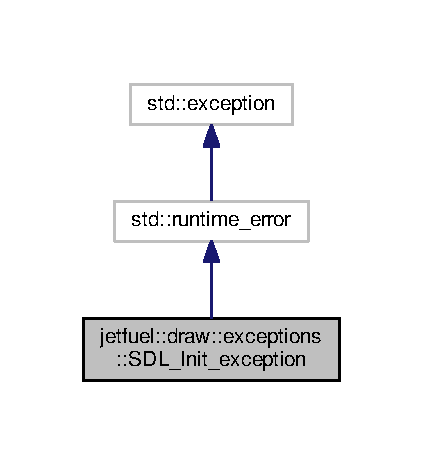
\includegraphics[width=203pt]{classjetfuel_1_1draw_1_1exceptions_1_1SDL__Init__exception__inherit__graph}
\end{center}
\end{figure}


Collaboration diagram for jetfuel\+:\+:draw\+:\+:exceptions\+:\+:S\+D\+L\+\_\+\+Init\+\_\+exception\+:
\nopagebreak
\begin{figure}[H]
\begin{center}
\leavevmode
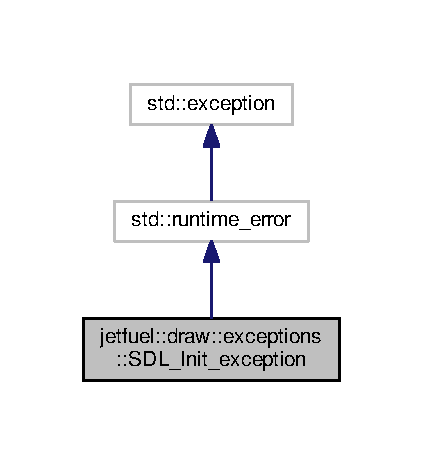
\includegraphics[width=203pt]{classjetfuel_1_1draw_1_1exceptions_1_1SDL__Init__exception__coll__graph}
\end{center}
\end{figure}
\subsection*{Public Member Functions}
\begin{DoxyCompactItemize}
\item 
\hyperlink{classjetfuel_1_1draw_1_1exceptions_1_1SDL__Init__exception_a7af9e4d40d575a1bec7b79407e2f7cce}{S\+D\+L\+\_\+\+Init\+\_\+exception} (const std\+::string sdl\+\_\+initerror)
\begin{DoxyCompactList}\small\item\em Constructs an \hyperlink{classjetfuel_1_1draw_1_1exceptions_1_1SDL__Init__exception}{S\+D\+L\+\_\+\+Init\+\_\+exception} with the error text. \end{DoxyCompactList}\end{DoxyCompactItemize}


\subsection{Detailed Description}
An exception to throw when the S\+DL initialize function S\+D\+L\+\_\+\+Init fails.

Code Example\+: if(S\+D\+L\+\_\+\+Init(\+S\+D\+L\+\_\+\+I\+N\+I\+T\+\_\+\+V\+I\+D\+E\+O) != 0)\{ throw exceptions\+::\+S\+D\+L\+\_\+\+Init\+\_\+exception(\+S\+D\+L\+\_\+\+Get\+Error()); \} 

\subsection{Constructor \& Destructor Documentation}
\mbox{\Hypertarget{classjetfuel_1_1draw_1_1exceptions_1_1SDL__Init__exception_a7af9e4d40d575a1bec7b79407e2f7cce}\label{classjetfuel_1_1draw_1_1exceptions_1_1SDL__Init__exception_a7af9e4d40d575a1bec7b79407e2f7cce}} 
\index{jetfuel\+::draw\+::exceptions\+::\+S\+D\+L\+\_\+\+Init\+\_\+exception@{jetfuel\+::draw\+::exceptions\+::\+S\+D\+L\+\_\+\+Init\+\_\+exception}!S\+D\+L\+\_\+\+Init\+\_\+exception@{S\+D\+L\+\_\+\+Init\+\_\+exception}}
\index{S\+D\+L\+\_\+\+Init\+\_\+exception@{S\+D\+L\+\_\+\+Init\+\_\+exception}!jetfuel\+::draw\+::exceptions\+::\+S\+D\+L\+\_\+\+Init\+\_\+exception@{jetfuel\+::draw\+::exceptions\+::\+S\+D\+L\+\_\+\+Init\+\_\+exception}}
\subsubsection{\texorpdfstring{S\+D\+L\+\_\+\+Init\+\_\+exception()}{SDL\_Init\_exception()}}
{\footnotesize\ttfamily jetfuel\+::draw\+::exceptions\+::\+S\+D\+L\+\_\+\+Init\+\_\+exception\+::\+S\+D\+L\+\_\+\+Init\+\_\+exception (\begin{DoxyParamCaption}\item[{const std\+::string}]{sdl\+\_\+initerror }\end{DoxyParamCaption})\hspace{0.3cm}{\ttfamily [inline]}}



Constructs an \hyperlink{classjetfuel_1_1draw_1_1exceptions_1_1SDL__Init__exception}{S\+D\+L\+\_\+\+Init\+\_\+exception} with the error text. 

Constructs an \hyperlink{classjetfuel_1_1draw_1_1exceptions_1_1SDL__Init__exception}{S\+D\+L\+\_\+\+Init\+\_\+exception} with the error text. 

The documentation for this class was generated from the following file\+:\begin{DoxyCompactItemize}
\item 
include/jetfueldraw/scenemanager.\+h\end{DoxyCompactItemize}

\hypertarget{classjetfuel_1_1media_1_1exceptions_1_1SDL__mixer__init__exception}{}\section{jetfuel\+:\+:media\+:\+:exceptions\+:\+:S\+D\+L\+\_\+mixer\+\_\+init\+\_\+exception Class Reference}
\label{classjetfuel_1_1media_1_1exceptions_1_1SDL__mixer__init__exception}\index{jetfuel\+::media\+::exceptions\+::\+S\+D\+L\+\_\+mixer\+\_\+init\+\_\+exception@{jetfuel\+::media\+::exceptions\+::\+S\+D\+L\+\_\+mixer\+\_\+init\+\_\+exception}}


{\ttfamily \#include $<$sound.\+h$>$}



Inheritance diagram for jetfuel\+:\+:media\+:\+:exceptions\+:\+:S\+D\+L\+\_\+mixer\+\_\+init\+\_\+exception\+:\nopagebreak
\begin{figure}[H]
\begin{center}
\leavevmode
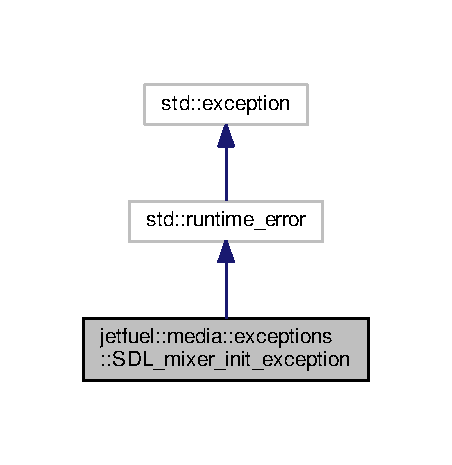
\includegraphics[width=217pt]{classjetfuel_1_1media_1_1exceptions_1_1SDL__mixer__init__exception__inherit__graph}
\end{center}
\end{figure}


Collaboration diagram for jetfuel\+:\+:media\+:\+:exceptions\+:\+:S\+D\+L\+\_\+mixer\+\_\+init\+\_\+exception\+:\nopagebreak
\begin{figure}[H]
\begin{center}
\leavevmode
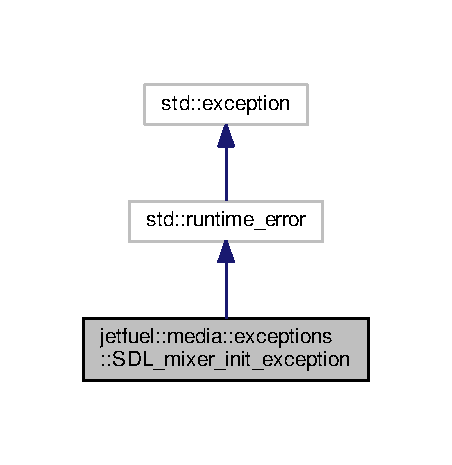
\includegraphics[width=217pt]{classjetfuel_1_1media_1_1exceptions_1_1SDL__mixer__init__exception__coll__graph}
\end{center}
\end{figure}
\subsection*{Public Member Functions}
\begin{DoxyCompactItemize}
\item 
\hyperlink{classjetfuel_1_1media_1_1exceptions_1_1SDL__mixer__init__exception_ad590081466a937313ebd7533a2a19692}{S\+D\+L\+\_\+mixer\+\_\+init\+\_\+exception} ()
\begin{DoxyCompactList}\small\item\em Default constructor. \end{DoxyCompactList}\end{DoxyCompactItemize}


\subsection{Detailed Description}
An exception thrown when initializing S\+D\+L\+\_\+mixer fails.

\begin{DoxySeeAlso}{See also}
\hyperlink{classjetfuel_1_1media_1_1Sound}{jetfuel\+::media\+::\+Sound} 

\hyperlink{classjetfuel_1_1media_1_1Music}{jetfuel\+::media\+::\+Music} 

\hyperlink{classjetfuel_1_1media_1_1Sound__effect}{jetfuel\+::media\+::\+Sound\+\_\+effect} 
\end{DoxySeeAlso}


\subsection{Constructor \& Destructor Documentation}
\mbox{\Hypertarget{classjetfuel_1_1media_1_1exceptions_1_1SDL__mixer__init__exception_ad590081466a937313ebd7533a2a19692}\label{classjetfuel_1_1media_1_1exceptions_1_1SDL__mixer__init__exception_ad590081466a937313ebd7533a2a19692}} 
\index{jetfuel\+::media\+::exceptions\+::\+S\+D\+L\+\_\+mixer\+\_\+init\+\_\+exception@{jetfuel\+::media\+::exceptions\+::\+S\+D\+L\+\_\+mixer\+\_\+init\+\_\+exception}!S\+D\+L\+\_\+mixer\+\_\+init\+\_\+exception@{S\+D\+L\+\_\+mixer\+\_\+init\+\_\+exception}}
\index{S\+D\+L\+\_\+mixer\+\_\+init\+\_\+exception@{S\+D\+L\+\_\+mixer\+\_\+init\+\_\+exception}!jetfuel\+::media\+::exceptions\+::\+S\+D\+L\+\_\+mixer\+\_\+init\+\_\+exception@{jetfuel\+::media\+::exceptions\+::\+S\+D\+L\+\_\+mixer\+\_\+init\+\_\+exception}}
\subsubsection{\texorpdfstring{S\+D\+L\+\_\+mixer\+\_\+init\+\_\+exception()}{SDL\_mixer\_init\_exception()}}
{\footnotesize\ttfamily jetfuel\+::media\+::exceptions\+::\+S\+D\+L\+\_\+mixer\+\_\+init\+\_\+exception\+::\+S\+D\+L\+\_\+mixer\+\_\+init\+\_\+exception (\begin{DoxyParamCaption}{ }\end{DoxyParamCaption})\hspace{0.3cm}{\ttfamily [inline]}}



Default constructor. 

Default constructor. 

The documentation for this class was generated from the following file\+:\begin{DoxyCompactItemize}
\item 
include/jetfuelmedia/sound.\+h\end{DoxyCompactItemize}

\hypertarget{classjetfuel_1_1draw_1_1exceptions_1_1SDL__ttf__exception}{}\section{jetfuel\+:\+:draw\+:\+:exceptions\+:\+:S\+D\+L\+\_\+ttf\+\_\+exception Class Reference}
\label{classjetfuel_1_1draw_1_1exceptions_1_1SDL__ttf__exception}\index{jetfuel\+::draw\+::exceptions\+::\+S\+D\+L\+\_\+ttf\+\_\+exception@{jetfuel\+::draw\+::exceptions\+::\+S\+D\+L\+\_\+ttf\+\_\+exception}}


{\ttfamily \#include $<$font.\+h$>$}



Inheritance diagram for jetfuel\+:\+:draw\+:\+:exceptions\+:\+:S\+D\+L\+\_\+ttf\+\_\+exception\+:\nopagebreak
\begin{figure}[H]
\begin{center}
\leavevmode
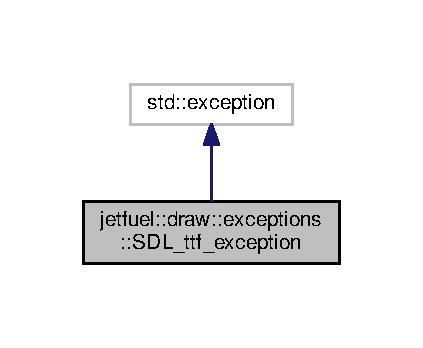
\includegraphics[width=203pt]{classjetfuel_1_1draw_1_1exceptions_1_1SDL__ttf__exception__inherit__graph}
\end{center}
\end{figure}


Collaboration diagram for jetfuel\+:\+:draw\+:\+:exceptions\+:\+:S\+D\+L\+\_\+ttf\+\_\+exception\+:\nopagebreak
\begin{figure}[H]
\begin{center}
\leavevmode
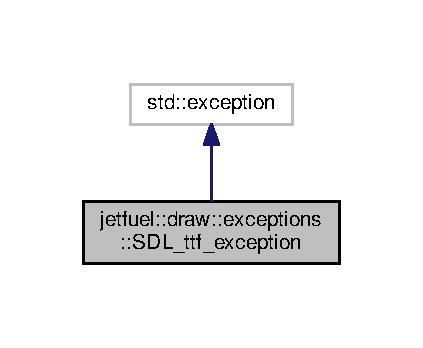
\includegraphics[width=203pt]{classjetfuel_1_1draw_1_1exceptions_1_1SDL__ttf__exception__coll__graph}
\end{center}
\end{figure}
\subsection*{Public Member Functions}
\begin{DoxyCompactItemize}
\item 
\mbox{\Hypertarget{classjetfuel_1_1draw_1_1exceptions_1_1SDL__ttf__exception_a55dd657b789c9df2b3373ce5d671e79a}\label{classjetfuel_1_1draw_1_1exceptions_1_1SDL__ttf__exception_a55dd657b789c9df2b3373ce5d671e79a}} 
virtual const char $\ast$ {\bfseries what} () const  throw ()
\end{DoxyCompactItemize}


\subsection{Detailed Description}
An exception to be thrown whenever a S\+D\+L\+\_\+\+T\+TF action done within a \hyperlink{classjetfuel_1_1draw_1_1Font}{Font} or \hyperlink{classjetfuel_1_1draw_1_1Text}{Text} object fails.

Code Example\+: 
\begin{DoxyCode}
\textcolor{keywordflow}{if}(TTF\_Init() < 0)\{
    \textcolor{keywordflow}{throw} exceptions::SDL\_ttf\_exception(\textcolor{stringliteral}{"TTF\_Init()"});
\}
\end{DoxyCode}
 

The documentation for this class was generated from the following file\+:\begin{DoxyCompactItemize}
\item 
include/jetfueldraw/font.\+h\end{DoxyCompactItemize}

\hypertarget{classjetfuel_1_1gui_1_1Slider}{}\section{jetfuel\+:\+:gui\+:\+:Slider Class Reference}
\label{classjetfuel_1_1gui_1_1Slider}\index{jetfuel\+::gui\+::\+Slider@{jetfuel\+::gui\+::\+Slider}}


{\ttfamily \#include $<$slider.\+h$>$}



Inheritance diagram for jetfuel\+:\+:gui\+:\+:Slider\+:\nopagebreak
\begin{figure}[H]
\begin{center}
\leavevmode
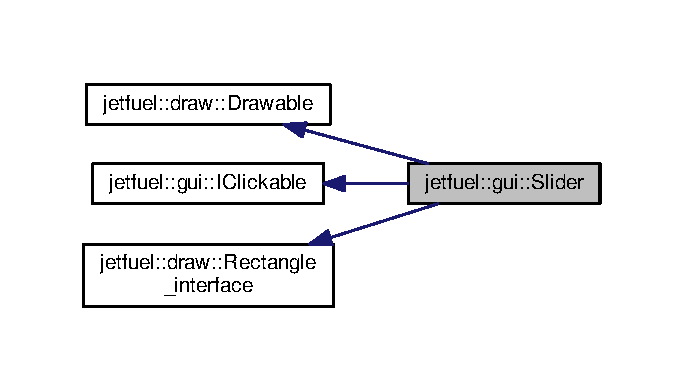
\includegraphics[width=328pt]{classjetfuel_1_1gui_1_1Slider__inherit__graph}
\end{center}
\end{figure}


Collaboration diagram for jetfuel\+:\+:gui\+:\+:Slider\+:\nopagebreak
\begin{figure}[H]
\begin{center}
\leavevmode
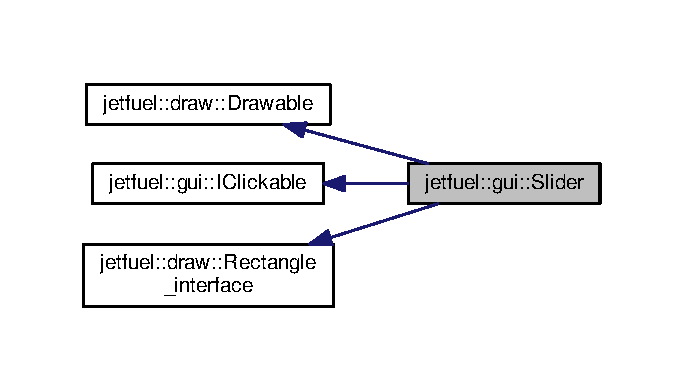
\includegraphics[width=328pt]{classjetfuel_1_1gui_1_1Slider__coll__graph}
\end{center}
\end{figure}
\subsection*{Public Member Functions}
\begin{DoxyCompactItemize}
\item 
\hyperlink{classjetfuel_1_1gui_1_1Slider_a961a11496cee6ab2f38aef1e14e94922}{Slider} ()
\begin{DoxyCompactList}\small\item\em Default constructor. \end{DoxyCompactList}\item 
\hyperlink{structjetfuel_1_1draw_1_1Rectangle__2d__shape_1_1Rectangle__2d__shape__characteristics}{jetfuel\+::draw\+::\+Rectangle\+\_\+2d\+\_\+shape\+::\+Rectangle\+\_\+2d\+\_\+shape\+\_\+characteristics} \hyperlink{classjetfuel_1_1gui_1_1Slider_aa7ca69b0cac43c29a9df8b2215c073bc}{Get\+\_\+slider\+\_\+rail\+\_\+characteristics} () const
\begin{DoxyCompactList}\small\item\em Gets the slider rail\textquotesingle{}s rectangular characteristics. \end{DoxyCompactList}\item 
void \hyperlink{classjetfuel_1_1gui_1_1Slider_a2cd13b87b896c03771bcdc29df1e1fc6}{Set\+\_\+slider\+\_\+rail\+\_\+characteristics} (\hyperlink{structjetfuel_1_1draw_1_1Rectangle__2d__shape_1_1Rectangle__2d__shape__characteristics}{jetfuel\+::draw\+::\+Rectangle\+\_\+2d\+\_\+shape\+::\+Rectangle\+\_\+2d\+\_\+shape\+\_\+characteristics} sliderrailcharacteristics)
\begin{DoxyCompactList}\small\item\em Sets the slider rail\textquotesingle{}s rectangular characteristics. \end{DoxyCompactList}\item 
\hyperlink{structjetfuel_1_1draw_1_1Circle__2d__shape_1_1Circle__2d__shape__characteristics}{jetfuel\+::draw\+::\+Circle\+\_\+2d\+\_\+shape\+::\+Circle\+\_\+2d\+\_\+shape\+\_\+characteristics} \hyperlink{classjetfuel_1_1gui_1_1Slider_a179af5f98738a5011b8608e656fdb090}{Get\+\_\+slider\+\_\+button\+\_\+characteristics} ()
\begin{DoxyCompactList}\small\item\em Gets the slider button\textquotesingle{}s circular button characteristics. \end{DoxyCompactList}\item 
void \hyperlink{classjetfuel_1_1gui_1_1Slider_a1d83644e298afe4153c00203ab493397}{Set\+\_\+slider\+\_\+button\+\_\+characteristics} (\hyperlink{structjetfuel_1_1draw_1_1Circle__2d__shape_1_1Circle__2d__shape__characteristics}{jetfuel\+::draw\+::\+Circle\+\_\+2d\+\_\+shape\+::\+Circle\+\_\+2d\+\_\+shape\+\_\+characteristics} sliderbuttoncharacteristics)
\begin{DoxyCompactList}\small\item\em Sets the slider button\textquotesingle{}s circular button characteristics. \end{DoxyCompactList}\item 
unsigned int \hyperlink{classjetfuel_1_1gui_1_1Slider_a6cb71758be2833e86c9fc80c457b4b24}{Get\+\_\+number\+\_\+of\+\_\+statuses} () const
\begin{DoxyCompactList}\small\item\em Gets the current number of possible statuses. \end{DoxyCompactList}\item 
void \hyperlink{classjetfuel_1_1gui_1_1Slider_abf6238d5bd9c33e2a22f5e901b62801d}{Set\+\_\+number\+\_\+of\+\_\+statuses} (const unsigned int statusnumber)
\begin{DoxyCompactList}\small\item\em Sets the current number of possible statuses. \end{DoxyCompactList}\item 
unsigned int \hyperlink{classjetfuel_1_1gui_1_1Slider_a62ef1133fbbea679b51d7ecf4ba4b6a8}{Get\+\_\+current\+\_\+status} () const
\begin{DoxyCompactList}\small\item\em Gets the current status of this \hyperlink{classjetfuel_1_1gui_1_1Slider}{Slider}. \end{DoxyCompactList}\item 
void \hyperlink{classjetfuel_1_1gui_1_1Slider_aa7a8125e92817f0df7899cc23f34fce7}{Set\+\_\+current\+\_\+status} (const unsigned int currentstatus)
\begin{DoxyCompactList}\small\item\em Sets the current status of this \hyperlink{classjetfuel_1_1gui_1_1Slider}{Slider}. \end{DoxyCompactList}\item 
\hyperlink{structjetfuel_1_1control_1_1UIS__input__actions}{jetfuel\+::control\+::\+U\+I\+S\+\_\+input\+\_\+actions} \hyperlink{classjetfuel_1_1gui_1_1Slider_a65b6eea54c4b4b78d0522b9eda83db0b}{Get\+\_\+control\+\_\+scheme} () const
\begin{DoxyCompactList}\small\item\em Gets the current control scheme of this \hyperlink{classjetfuel_1_1gui_1_1Slider}{Slider}. \end{DoxyCompactList}\item 
void \hyperlink{classjetfuel_1_1gui_1_1Slider_a64531a8ed9353906ffb8e1b5720e9409}{Set\+\_\+control\+\_\+scheme} (\hyperlink{structjetfuel_1_1control_1_1UIS__input__actions}{jetfuel\+::control\+::\+U\+I\+S\+\_\+input\+\_\+actions} U\+I\+Scontrols)
\begin{DoxyCompactList}\small\item\em Sets the current control scheme of this \hyperlink{classjetfuel_1_1gui_1_1Slider}{Slider}. \end{DoxyCompactList}\item 
void \hyperlink{classjetfuel_1_1gui_1_1Slider_af9ceba04fec0f7cdc097ea0513094176}{Assign\+\_\+renderer} (S\+D\+L\+\_\+\+Renderer $\ast$renderer) override
\begin{DoxyCompactList}\small\item\em Assigns a renderer to this \hyperlink{classjetfuel_1_1gui_1_1Slider}{Slider}. \end{DoxyCompactList}\item 
\hyperlink{classjetfuel_1_1draw_1_1Vector2d}{jetfuel\+::draw\+::\+Vector2d\+\_\+int} \hyperlink{classjetfuel_1_1gui_1_1Slider_a2b177c832a42ad21ca1fa88496ef7551}{Get\+\_\+position} () override
\begin{DoxyCompactList}\small\item\em Gets this \hyperlink{classjetfuel_1_1gui_1_1Slider}{Slider}\textquotesingle{}s position. \end{DoxyCompactList}\item 
void \hyperlink{classjetfuel_1_1gui_1_1Slider_a11721a72699e9d1cdd0f6e5709f003e4}{Set\+\_\+position} (\hyperlink{classjetfuel_1_1draw_1_1Vector2d}{jetfuel\+::draw\+::\+Vector2d\+\_\+int} position) override
\begin{DoxyCompactList}\small\item\em Sets this \hyperlink{classjetfuel_1_1gui_1_1Slider}{Slider}\textquotesingle{}s position. \end{DoxyCompactList}\item 
\hyperlink{classjetfuel_1_1draw_1_1Rect2d}{jetfuel\+::draw\+::\+Rect2d\+\_\+int} \hyperlink{classjetfuel_1_1gui_1_1Slider_abab31dbe01b716b4e82919f0d8aba96c}{Get\+\_\+rect\+\_\+to\+\_\+draw} () override
\begin{DoxyCompactList}\small\item\em Gets this \hyperlink{classjetfuel_1_1gui_1_1Slider}{Slider}\textquotesingle{}s rect to draw when the Draw function is called. \end{DoxyCompactList}\item 
void \hyperlink{classjetfuel_1_1gui_1_1Slider_a8a1e83cfea8d65db34da7447dce9fb6f}{Check\+\_\+for\+\_\+clicks} (\hyperlink{structjetfuel_1_1control_1_1Action}{jetfuel\+::control\+::\+Action} U\+I\+Sinterpreterdata) override
\begin{DoxyCompactList}\small\item\em Checks for clicks on this \hyperlink{classjetfuel_1_1gui_1_1Slider}{Slider}. \end{DoxyCompactList}\item 
bool \hyperlink{classjetfuel_1_1gui_1_1Slider_a483038c689276ed8468e990977e5a74a}{Draw} () override
\begin{DoxyCompactList}\small\item\em Draws this \hyperlink{classjetfuel_1_1gui_1_1Slider}{Slider} onto the screen. \end{DoxyCompactList}\end{DoxyCompactItemize}
\subsection*{Protected Member Functions}
\begin{DoxyCompactItemize}
\item 
void \hyperlink{classjetfuel_1_1gui_1_1Slider_ae0b83862beb7f631145fd3c9dddfb661}{Set\+\_\+slider\+\_\+button\+\_\+position} (\hyperlink{classjetfuel_1_1draw_1_1Vector2d}{jetfuel\+::draw\+::\+Vector2d\+\_\+int} position)
\begin{DoxyCompactList}\small\item\em Sets the slider button\textquotesingle{}s position. \end{DoxyCompactList}\item 
bool \hyperlink{classjetfuel_1_1gui_1_1Slider_a730d18fe513120406907380b7caf3280}{Draw\+\_\+slider\+\_\+member\+\_\+objects} ()
\begin{DoxyCompactList}\small\item\em Draws this slider\textquotesingle{}s member objects. \end{DoxyCompactList}\item 
int \hyperlink{classjetfuel_1_1gui_1_1Slider_a4115f54db7955a6493661ec176b532fd}{Get\+\_\+width\+\_\+of\+\_\+slider\+\_\+rail} ()
\begin{DoxyCompactList}\small\item\em Gets the width of the slider rail. \end{DoxyCompactList}\end{DoxyCompactItemize}


\subsection{Detailed Description}
A simple slider G\+UI class that allows the user to pick different spots on a line represesenting different statuses(or, potentially, actions).

Code Example\+: 
\begin{DoxyCode}
\hyperlink{classjetfuel_1_1draw_1_1Scene__manager}{jetfuel::draw::Scene\_manager} scenemanager;
\hyperlink{classjetfuel_1_1draw_1_1Scene}{jetfuel::draw::Scene} scene1(1);
\hyperlink{classjetfuel_1_1core_1_1Message__bus}{jetfuel::core::Message\_bus} messagebus;
\hyperlink{classjetfuel_1_1gui_1_1Slider}{jetfuel::gui::Slider} slider;
\hyperlink{classjetfuel_1_1control_1_1UIS__manager}{jetfuel::control::UIS\_manager} UISmanager(&messagebus,
                                  scenemanager.\hyperlink{classjetfuel_1_1draw_1_1Scene__manager_a1758a86d40dcfaface8958fcd33676bf}{Get\_window\_id}());
\hyperlink{classjetfuel_1_1control_1_1UIS__interpreter}{jetfuel::control::UIS\_interpreter} UISinterpreter(&messagebus);
\hyperlink{structjetfuel_1_1control_1_1UIS__input__actions}{jetfuel::control::UIS\_input\_actions} UISinputactions;
\hyperlink{classjetfuel_1_1draw_1_1Font}{jetfuel::draw::Font} font(\textcolor{stringliteral}{"default.ttf"});

\textcolor{keywordflow}{if}(!scenemanager.\hyperlink{classjetfuel_1_1draw_1_1Scene__manager_a5113e9062c272a22d383ba872417ba31}{Create\_window}(\textcolor{stringliteral}{"Hello Sliders!"},
                               \hyperlink{classjetfuel_1_1draw_1_1Vector2d}{jetfuel::draw::Vector2d\_int}(0,0),
                          \hyperlink{classjetfuel_1_1draw_1_1Vector2d}{jetfuel::draw::Vector2d\_int}(640,480)))\{
    std::cout << \textcolor{stringliteral}{"[!]ERROR with creating sdl window! Error is:"}
    << SDL\_GetError() << \textcolor{stringliteral}{"\(\backslash\)n"};
\}

\textcolor{keywordflow}{if}(!scenemanager.\hyperlink{classjetfuel_1_1draw_1_1Scene__manager_afafecd926ce5e4b2543a6d583a7d24b6}{Create\_renderer}())\{
    std::cout << \textcolor{stringliteral}{"[!]ERROR with creating sdl renderer! Error is:"}
    << SDL\_GetError() << \textcolor{stringliteral}{"\(\backslash\)n"};
\}
scenemanager.\hyperlink{classjetfuel_1_1draw_1_1Scene__manager_a770c163b88ba8427539ee182315ea989}{Switch\_current\_scene}(&scene1);
scene1.\hyperlink{classjetfuel_1_1draw_1_1Scene_aea4b4c4ae25c30d661be4c52787e0ea3}{Attach\_drawable}(&slider,1);

slider.\hyperlink{classjetfuel_1_1gui_1_1Slider_a11721a72699e9d1cdd0f6e5709f003e4}{Set\_position}(\hyperlink{classjetfuel_1_1draw_1_1Vector2d}{jetfuel::draw::Vector2d\_int}(0,0));

slider.Set\_current\_status\_number(0); \textcolor{comment}{// zero-indexed}
slider.Set\_max\_number\_of\_statuses(4);

UISinputactions.mousemessagetowatch = &messagebus;

slider.\hyperlink{classjetfuel_1_1gui_1_1Slider_a64531a8ed9353906ffb8e1b5720e9409}{Set\_control\_scheme}(UISinputactions);

scenemanager.\hyperlink{classjetfuel_1_1draw_1_1Scene__manager_a8af9a3abfd5121b1b8556342de435773}{Draw\_current\_scene}();
\end{DoxyCode}
 

\subsection{Constructor \& Destructor Documentation}
\mbox{\Hypertarget{classjetfuel_1_1gui_1_1Slider_a961a11496cee6ab2f38aef1e14e94922}\label{classjetfuel_1_1gui_1_1Slider_a961a11496cee6ab2f38aef1e14e94922}} 
\index{jetfuel\+::gui\+::\+Slider@{jetfuel\+::gui\+::\+Slider}!Slider@{Slider}}
\index{Slider@{Slider}!jetfuel\+::gui\+::\+Slider@{jetfuel\+::gui\+::\+Slider}}
\subsubsection{\texorpdfstring{Slider()}{Slider()}}
{\footnotesize\ttfamily jetfuel\+::gui\+::\+Slider\+::\+Slider (\begin{DoxyParamCaption}{ }\end{DoxyParamCaption})\hspace{0.3cm}{\ttfamily [inline]}}



Default constructor. 

Default constructor. 

\subsection{Member Function Documentation}
\mbox{\Hypertarget{classjetfuel_1_1gui_1_1Slider_af9ceba04fec0f7cdc097ea0513094176}\label{classjetfuel_1_1gui_1_1Slider_af9ceba04fec0f7cdc097ea0513094176}} 
\index{jetfuel\+::gui\+::\+Slider@{jetfuel\+::gui\+::\+Slider}!Assign\+\_\+renderer@{Assign\+\_\+renderer}}
\index{Assign\+\_\+renderer@{Assign\+\_\+renderer}!jetfuel\+::gui\+::\+Slider@{jetfuel\+::gui\+::\+Slider}}
\subsubsection{\texorpdfstring{Assign\+\_\+renderer()}{Assign\_renderer()}}
{\footnotesize\ttfamily void jetfuel\+::gui\+::\+Slider\+::\+Assign\+\_\+renderer (\begin{DoxyParamCaption}\item[{S\+D\+L\+\_\+\+Renderer $\ast$}]{renderer }\end{DoxyParamCaption})\hspace{0.3cm}{\ttfamily [inline]}, {\ttfamily [override]}, {\ttfamily [virtual]}}



Assigns a renderer to this \hyperlink{classjetfuel_1_1gui_1_1Slider}{Slider}. 

Assigns a renderer to this \hyperlink{classjetfuel_1_1gui_1_1Slider}{Slider}.


\begin{DoxyParams}{Parameters}
{\em S\+D\+L\+\_\+\+Renderer} & $\ast$renderer \\
\hline
\end{DoxyParams}


Reimplemented from \hyperlink{classjetfuel_1_1draw_1_1Drawable_a0d7257f197d6ffcdd89c3a99c93d1400}{jetfuel\+::draw\+::\+Drawable}.

\mbox{\Hypertarget{classjetfuel_1_1gui_1_1Slider_a8a1e83cfea8d65db34da7447dce9fb6f}\label{classjetfuel_1_1gui_1_1Slider_a8a1e83cfea8d65db34da7447dce9fb6f}} 
\index{jetfuel\+::gui\+::\+Slider@{jetfuel\+::gui\+::\+Slider}!Check\+\_\+for\+\_\+clicks@{Check\+\_\+for\+\_\+clicks}}
\index{Check\+\_\+for\+\_\+clicks@{Check\+\_\+for\+\_\+clicks}!jetfuel\+::gui\+::\+Slider@{jetfuel\+::gui\+::\+Slider}}
\subsubsection{\texorpdfstring{Check\+\_\+for\+\_\+clicks()}{Check\_for\_clicks()}}
{\footnotesize\ttfamily void jetfuel\+::gui\+::\+Slider\+::\+Check\+\_\+for\+\_\+clicks (\begin{DoxyParamCaption}\item[{\hyperlink{structjetfuel_1_1control_1_1Action}{jetfuel\+::control\+::\+Action}}]{U\+I\+Sinterpreterdata }\end{DoxyParamCaption})\hspace{0.3cm}{\ttfamily [override]}, {\ttfamily [virtual]}}



Checks for clicks on this \hyperlink{classjetfuel_1_1gui_1_1Slider}{Slider}. 

Checks for clicks on this \hyperlink{classjetfuel_1_1gui_1_1Slider}{Slider}.


\begin{DoxyParams}{Parameters}
{\em \hyperlink{structjetfuel_1_1control_1_1Action}{jetfuel\+::control\+::\+Action}} & U\+I\+Sinterpreterdata \\
\hline
\end{DoxyParams}


Implements \hyperlink{classjetfuel_1_1gui_1_1IClickable_aea45de37bd3beb7eb7e2e3056e4e37b3}{jetfuel\+::gui\+::\+I\+Clickable}.

\mbox{\Hypertarget{classjetfuel_1_1gui_1_1Slider_a483038c689276ed8468e990977e5a74a}\label{classjetfuel_1_1gui_1_1Slider_a483038c689276ed8468e990977e5a74a}} 
\index{jetfuel\+::gui\+::\+Slider@{jetfuel\+::gui\+::\+Slider}!Draw@{Draw}}
\index{Draw@{Draw}!jetfuel\+::gui\+::\+Slider@{jetfuel\+::gui\+::\+Slider}}
\subsubsection{\texorpdfstring{Draw()}{Draw()}}
{\footnotesize\ttfamily bool jetfuel\+::gui\+::\+Slider\+::\+Draw (\begin{DoxyParamCaption}{ }\end{DoxyParamCaption})\hspace{0.3cm}{\ttfamily [override]}, {\ttfamily [virtual]}}



Draws this \hyperlink{classjetfuel_1_1gui_1_1Slider}{Slider} onto the screen. 

Draws this \hyperlink{classjetfuel_1_1gui_1_1Slider}{Slider} onto the screen. 

Implements \hyperlink{classjetfuel_1_1draw_1_1Drawable_a1a072070322965ce9411ee6e7c311c56}{jetfuel\+::draw\+::\+Drawable}.

\mbox{\Hypertarget{classjetfuel_1_1gui_1_1Slider_a730d18fe513120406907380b7caf3280}\label{classjetfuel_1_1gui_1_1Slider_a730d18fe513120406907380b7caf3280}} 
\index{jetfuel\+::gui\+::\+Slider@{jetfuel\+::gui\+::\+Slider}!Draw\+\_\+slider\+\_\+member\+\_\+objects@{Draw\+\_\+slider\+\_\+member\+\_\+objects}}
\index{Draw\+\_\+slider\+\_\+member\+\_\+objects@{Draw\+\_\+slider\+\_\+member\+\_\+objects}!jetfuel\+::gui\+::\+Slider@{jetfuel\+::gui\+::\+Slider}}
\subsubsection{\texorpdfstring{Draw\+\_\+slider\+\_\+member\+\_\+objects()}{Draw\_slider\_member\_objects()}}
{\footnotesize\ttfamily bool jetfuel\+::gui\+::\+Slider\+::\+Draw\+\_\+slider\+\_\+member\+\_\+objects (\begin{DoxyParamCaption}{ }\end{DoxyParamCaption})\hspace{0.3cm}{\ttfamily [inline]}, {\ttfamily [protected]}}



Draws this slider\textquotesingle{}s member objects. 

Draws this slider\textquotesingle{}s member objects (i.\+e. the slider rail, the slider button). \mbox{\Hypertarget{classjetfuel_1_1gui_1_1Slider_a65b6eea54c4b4b78d0522b9eda83db0b}\label{classjetfuel_1_1gui_1_1Slider_a65b6eea54c4b4b78d0522b9eda83db0b}} 
\index{jetfuel\+::gui\+::\+Slider@{jetfuel\+::gui\+::\+Slider}!Get\+\_\+control\+\_\+scheme@{Get\+\_\+control\+\_\+scheme}}
\index{Get\+\_\+control\+\_\+scheme@{Get\+\_\+control\+\_\+scheme}!jetfuel\+::gui\+::\+Slider@{jetfuel\+::gui\+::\+Slider}}
\subsubsection{\texorpdfstring{Get\+\_\+control\+\_\+scheme()}{Get\_control\_scheme()}}
{\footnotesize\ttfamily \hyperlink{structjetfuel_1_1control_1_1UIS__input__actions}{jetfuel\+::control\+::\+U\+I\+S\+\_\+input\+\_\+actions} jetfuel\+::gui\+::\+Slider\+::\+Get\+\_\+control\+\_\+scheme (\begin{DoxyParamCaption}{ }\end{DoxyParamCaption}) const\hspace{0.3cm}{\ttfamily [inline]}}



Gets the current control scheme of this \hyperlink{classjetfuel_1_1gui_1_1Slider}{Slider}. 

Gets the current control scheme of this \hyperlink{classjetfuel_1_1gui_1_1Slider}{Slider}. \mbox{\Hypertarget{classjetfuel_1_1gui_1_1Slider_a62ef1133fbbea679b51d7ecf4ba4b6a8}\label{classjetfuel_1_1gui_1_1Slider_a62ef1133fbbea679b51d7ecf4ba4b6a8}} 
\index{jetfuel\+::gui\+::\+Slider@{jetfuel\+::gui\+::\+Slider}!Get\+\_\+current\+\_\+status@{Get\+\_\+current\+\_\+status}}
\index{Get\+\_\+current\+\_\+status@{Get\+\_\+current\+\_\+status}!jetfuel\+::gui\+::\+Slider@{jetfuel\+::gui\+::\+Slider}}
\subsubsection{\texorpdfstring{Get\+\_\+current\+\_\+status()}{Get\_current\_status()}}
{\footnotesize\ttfamily unsigned int jetfuel\+::gui\+::\+Slider\+::\+Get\+\_\+current\+\_\+status (\begin{DoxyParamCaption}{ }\end{DoxyParamCaption}) const\hspace{0.3cm}{\ttfamily [inline]}}



Gets the current status of this \hyperlink{classjetfuel_1_1gui_1_1Slider}{Slider}. 

Gets the current status of this \hyperlink{classjetfuel_1_1gui_1_1Slider}{Slider}. \mbox{\Hypertarget{classjetfuel_1_1gui_1_1Slider_a6cb71758be2833e86c9fc80c457b4b24}\label{classjetfuel_1_1gui_1_1Slider_a6cb71758be2833e86c9fc80c457b4b24}} 
\index{jetfuel\+::gui\+::\+Slider@{jetfuel\+::gui\+::\+Slider}!Get\+\_\+number\+\_\+of\+\_\+statuses@{Get\+\_\+number\+\_\+of\+\_\+statuses}}
\index{Get\+\_\+number\+\_\+of\+\_\+statuses@{Get\+\_\+number\+\_\+of\+\_\+statuses}!jetfuel\+::gui\+::\+Slider@{jetfuel\+::gui\+::\+Slider}}
\subsubsection{\texorpdfstring{Get\+\_\+number\+\_\+of\+\_\+statuses()}{Get\_number\_of\_statuses()}}
{\footnotesize\ttfamily unsigned int jetfuel\+::gui\+::\+Slider\+::\+Get\+\_\+number\+\_\+of\+\_\+statuses (\begin{DoxyParamCaption}{ }\end{DoxyParamCaption}) const\hspace{0.3cm}{\ttfamily [inline]}}



Gets the current number of possible statuses. 

Gets the current number of possible statuses. \mbox{\Hypertarget{classjetfuel_1_1gui_1_1Slider_a2b177c832a42ad21ca1fa88496ef7551}\label{classjetfuel_1_1gui_1_1Slider_a2b177c832a42ad21ca1fa88496ef7551}} 
\index{jetfuel\+::gui\+::\+Slider@{jetfuel\+::gui\+::\+Slider}!Get\+\_\+position@{Get\+\_\+position}}
\index{Get\+\_\+position@{Get\+\_\+position}!jetfuel\+::gui\+::\+Slider@{jetfuel\+::gui\+::\+Slider}}
\subsubsection{\texorpdfstring{Get\+\_\+position()}{Get\_position()}}
{\footnotesize\ttfamily \hyperlink{classjetfuel_1_1draw_1_1Vector2d}{jetfuel\+::draw\+::\+Vector2d\+\_\+int} jetfuel\+::gui\+::\+Slider\+::\+Get\+\_\+position (\begin{DoxyParamCaption}{ }\end{DoxyParamCaption})\hspace{0.3cm}{\ttfamily [inline]}, {\ttfamily [override]}, {\ttfamily [virtual]}}



Gets this \hyperlink{classjetfuel_1_1gui_1_1Slider}{Slider}\textquotesingle{}s position. 

Gets this \hyperlink{classjetfuel_1_1gui_1_1Slider}{Slider}\textquotesingle{}s position. 

Reimplemented from \hyperlink{classjetfuel_1_1draw_1_1Drawable_ae7ebd30d66db2c8a5d5371cbcf0023fc}{jetfuel\+::draw\+::\+Drawable}.

\mbox{\Hypertarget{classjetfuel_1_1gui_1_1Slider_abab31dbe01b716b4e82919f0d8aba96c}\label{classjetfuel_1_1gui_1_1Slider_abab31dbe01b716b4e82919f0d8aba96c}} 
\index{jetfuel\+::gui\+::\+Slider@{jetfuel\+::gui\+::\+Slider}!Get\+\_\+rect\+\_\+to\+\_\+draw@{Get\+\_\+rect\+\_\+to\+\_\+draw}}
\index{Get\+\_\+rect\+\_\+to\+\_\+draw@{Get\+\_\+rect\+\_\+to\+\_\+draw}!jetfuel\+::gui\+::\+Slider@{jetfuel\+::gui\+::\+Slider}}
\subsubsection{\texorpdfstring{Get\+\_\+rect\+\_\+to\+\_\+draw()}{Get\_rect\_to\_draw()}}
{\footnotesize\ttfamily \hyperlink{classjetfuel_1_1draw_1_1Rect2d}{jetfuel\+::draw\+::\+Rect2d\+\_\+int} jetfuel\+::gui\+::\+Slider\+::\+Get\+\_\+rect\+\_\+to\+\_\+draw (\begin{DoxyParamCaption}{ }\end{DoxyParamCaption})\hspace{0.3cm}{\ttfamily [inline]}, {\ttfamily [override]}, {\ttfamily [virtual]}}



Gets this \hyperlink{classjetfuel_1_1gui_1_1Slider}{Slider}\textquotesingle{}s rect to draw when the Draw function is called. 

Gets this \hyperlink{classjetfuel_1_1gui_1_1Slider}{Slider}\textquotesingle{}s rect to draw when the Draw function is called. 

Implements \hyperlink{classjetfuel_1_1draw_1_1Rectangle__interface_a03fd3b6842ab7b3065379caec407296f}{jetfuel\+::draw\+::\+Rectangle\+\_\+interface}.

\mbox{\Hypertarget{classjetfuel_1_1gui_1_1Slider_a179af5f98738a5011b8608e656fdb090}\label{classjetfuel_1_1gui_1_1Slider_a179af5f98738a5011b8608e656fdb090}} 
\index{jetfuel\+::gui\+::\+Slider@{jetfuel\+::gui\+::\+Slider}!Get\+\_\+slider\+\_\+button\+\_\+characteristics@{Get\+\_\+slider\+\_\+button\+\_\+characteristics}}
\index{Get\+\_\+slider\+\_\+button\+\_\+characteristics@{Get\+\_\+slider\+\_\+button\+\_\+characteristics}!jetfuel\+::gui\+::\+Slider@{jetfuel\+::gui\+::\+Slider}}
\subsubsection{\texorpdfstring{Get\+\_\+slider\+\_\+button\+\_\+characteristics()}{Get\_slider\_button\_characteristics()}}
{\footnotesize\ttfamily jetfuel\+::draw\+::\+Circle\+\_\+2d\+\_\+shape\+:: Circle\+\_\+2d\+\_\+shape\+\_\+characteristics jetfuel\+::gui\+::\+Slider\+::\+Get\+\_\+slider\+\_\+button\+\_\+characteristics (\begin{DoxyParamCaption}{ }\end{DoxyParamCaption})\hspace{0.3cm}{\ttfamily [inline]}}



Gets the slider button\textquotesingle{}s circular button characteristics. 

Gets the slider button\textquotesingle{}s circular button scharacteristics. \mbox{\Hypertarget{classjetfuel_1_1gui_1_1Slider_aa7ca69b0cac43c29a9df8b2215c073bc}\label{classjetfuel_1_1gui_1_1Slider_aa7ca69b0cac43c29a9df8b2215c073bc}} 
\index{jetfuel\+::gui\+::\+Slider@{jetfuel\+::gui\+::\+Slider}!Get\+\_\+slider\+\_\+rail\+\_\+characteristics@{Get\+\_\+slider\+\_\+rail\+\_\+characteristics}}
\index{Get\+\_\+slider\+\_\+rail\+\_\+characteristics@{Get\+\_\+slider\+\_\+rail\+\_\+characteristics}!jetfuel\+::gui\+::\+Slider@{jetfuel\+::gui\+::\+Slider}}
\subsubsection{\texorpdfstring{Get\+\_\+slider\+\_\+rail\+\_\+characteristics()}{Get\_slider\_rail\_characteristics()}}
{\footnotesize\ttfamily jetfuel\+::draw\+::\+Rectangle\+\_\+2d\+\_\+shape\+:: Rectangle\+\_\+2d\+\_\+shape\+\_\+characteristics jetfuel\+::gui\+::\+Slider\+::\+Get\+\_\+slider\+\_\+rail\+\_\+characteristics (\begin{DoxyParamCaption}{ }\end{DoxyParamCaption}) const\hspace{0.3cm}{\ttfamily [inline]}}



Gets the slider rail\textquotesingle{}s rectangular characteristics. 

Gets the slider rail\textquotesingle{}s rectangular characteristics. \mbox{\Hypertarget{classjetfuel_1_1gui_1_1Slider_a4115f54db7955a6493661ec176b532fd}\label{classjetfuel_1_1gui_1_1Slider_a4115f54db7955a6493661ec176b532fd}} 
\index{jetfuel\+::gui\+::\+Slider@{jetfuel\+::gui\+::\+Slider}!Get\+\_\+width\+\_\+of\+\_\+slider\+\_\+rail@{Get\+\_\+width\+\_\+of\+\_\+slider\+\_\+rail}}
\index{Get\+\_\+width\+\_\+of\+\_\+slider\+\_\+rail@{Get\+\_\+width\+\_\+of\+\_\+slider\+\_\+rail}!jetfuel\+::gui\+::\+Slider@{jetfuel\+::gui\+::\+Slider}}
\subsubsection{\texorpdfstring{Get\+\_\+width\+\_\+of\+\_\+slider\+\_\+rail()}{Get\_width\_of\_slider\_rail()}}
{\footnotesize\ttfamily int jetfuel\+::gui\+::\+Slider\+::\+Get\+\_\+width\+\_\+of\+\_\+slider\+\_\+rail (\begin{DoxyParamCaption}{ }\end{DoxyParamCaption})\hspace{0.3cm}{\ttfamily [inline]}, {\ttfamily [protected]}}



Gets the width of the slider rail. 

Gets the width of the slider rail. \mbox{\Hypertarget{classjetfuel_1_1gui_1_1Slider_a64531a8ed9353906ffb8e1b5720e9409}\label{classjetfuel_1_1gui_1_1Slider_a64531a8ed9353906ffb8e1b5720e9409}} 
\index{jetfuel\+::gui\+::\+Slider@{jetfuel\+::gui\+::\+Slider}!Set\+\_\+control\+\_\+scheme@{Set\+\_\+control\+\_\+scheme}}
\index{Set\+\_\+control\+\_\+scheme@{Set\+\_\+control\+\_\+scheme}!jetfuel\+::gui\+::\+Slider@{jetfuel\+::gui\+::\+Slider}}
\subsubsection{\texorpdfstring{Set\+\_\+control\+\_\+scheme()}{Set\_control\_scheme()}}
{\footnotesize\ttfamily void jetfuel\+::gui\+::\+Slider\+::\+Set\+\_\+control\+\_\+scheme (\begin{DoxyParamCaption}\item[{\hyperlink{structjetfuel_1_1control_1_1UIS__input__actions}{jetfuel\+::control\+::\+U\+I\+S\+\_\+input\+\_\+actions}}]{U\+I\+Scontrols }\end{DoxyParamCaption})\hspace{0.3cm}{\ttfamily [inline]}}



Sets the current control scheme of this \hyperlink{classjetfuel_1_1gui_1_1Slider}{Slider}. 

Sets the current control scheme of this \hyperlink{classjetfuel_1_1gui_1_1Slider}{Slider}.


\begin{DoxyParams}{Parameters}
{\em \hyperlink{structjetfuel_1_1control_1_1UIS__input__actions}{jetfuel\+::control\+::\+U\+I\+S\+\_\+input\+\_\+actions}} & \\
\hline
\end{DoxyParams}
\mbox{\Hypertarget{classjetfuel_1_1gui_1_1Slider_aa7a8125e92817f0df7899cc23f34fce7}\label{classjetfuel_1_1gui_1_1Slider_aa7a8125e92817f0df7899cc23f34fce7}} 
\index{jetfuel\+::gui\+::\+Slider@{jetfuel\+::gui\+::\+Slider}!Set\+\_\+current\+\_\+status@{Set\+\_\+current\+\_\+status}}
\index{Set\+\_\+current\+\_\+status@{Set\+\_\+current\+\_\+status}!jetfuel\+::gui\+::\+Slider@{jetfuel\+::gui\+::\+Slider}}
\subsubsection{\texorpdfstring{Set\+\_\+current\+\_\+status()}{Set\_current\_status()}}
{\footnotesize\ttfamily void jetfuel\+::gui\+::\+Slider\+::\+Set\+\_\+current\+\_\+status (\begin{DoxyParamCaption}\item[{const unsigned int}]{currentstatus }\end{DoxyParamCaption})\hspace{0.3cm}{\ttfamily [inline]}}



Sets the current status of this \hyperlink{classjetfuel_1_1gui_1_1Slider}{Slider}. 

Sets the current status of this \hyperlink{classjetfuel_1_1gui_1_1Slider}{Slider}. If this number is greater than the total number of statuses, it will be capped at that number.


\begin{DoxyParams}{Parameters}
{\em unsigned} & int currentstatus \\
\hline
\end{DoxyParams}
\mbox{\Hypertarget{classjetfuel_1_1gui_1_1Slider_abf6238d5bd9c33e2a22f5e901b62801d}\label{classjetfuel_1_1gui_1_1Slider_abf6238d5bd9c33e2a22f5e901b62801d}} 
\index{jetfuel\+::gui\+::\+Slider@{jetfuel\+::gui\+::\+Slider}!Set\+\_\+number\+\_\+of\+\_\+statuses@{Set\+\_\+number\+\_\+of\+\_\+statuses}}
\index{Set\+\_\+number\+\_\+of\+\_\+statuses@{Set\+\_\+number\+\_\+of\+\_\+statuses}!jetfuel\+::gui\+::\+Slider@{jetfuel\+::gui\+::\+Slider}}
\subsubsection{\texorpdfstring{Set\+\_\+number\+\_\+of\+\_\+statuses()}{Set\_number\_of\_statuses()}}
{\footnotesize\ttfamily void jetfuel\+::gui\+::\+Slider\+::\+Set\+\_\+number\+\_\+of\+\_\+statuses (\begin{DoxyParamCaption}\item[{const unsigned int}]{statusnumber }\end{DoxyParamCaption})\hspace{0.3cm}{\ttfamily [inline]}}



Sets the current number of possible statuses. 

Sets the current number of possible statuses.


\begin{DoxyParams}{Parameters}
{\em unsigned} & int statusnumber \\
\hline
\end{DoxyParams}
\mbox{\Hypertarget{classjetfuel_1_1gui_1_1Slider_a11721a72699e9d1cdd0f6e5709f003e4}\label{classjetfuel_1_1gui_1_1Slider_a11721a72699e9d1cdd0f6e5709f003e4}} 
\index{jetfuel\+::gui\+::\+Slider@{jetfuel\+::gui\+::\+Slider}!Set\+\_\+position@{Set\+\_\+position}}
\index{Set\+\_\+position@{Set\+\_\+position}!jetfuel\+::gui\+::\+Slider@{jetfuel\+::gui\+::\+Slider}}
\subsubsection{\texorpdfstring{Set\+\_\+position()}{Set\_position()}}
{\footnotesize\ttfamily void jetfuel\+::gui\+::\+Slider\+::\+Set\+\_\+position (\begin{DoxyParamCaption}\item[{\hyperlink{classjetfuel_1_1draw_1_1Vector2d}{jetfuel\+::draw\+::\+Vector2d\+\_\+int}}]{position }\end{DoxyParamCaption})\hspace{0.3cm}{\ttfamily [inline]}, {\ttfamily [override]}, {\ttfamily [virtual]}}



Sets this \hyperlink{classjetfuel_1_1gui_1_1Slider}{Slider}\textquotesingle{}s position. 

Sets this \hyperlink{classjetfuel_1_1gui_1_1Slider}{Slider}\textquotesingle{}s position.

jetfuel\+::draw\+::\+Vector2d\+\_\+int position 

Reimplemented from \hyperlink{classjetfuel_1_1draw_1_1Drawable_afdd035afe40c706459a6c9df813bcce6}{jetfuel\+::draw\+::\+Drawable}.

\mbox{\Hypertarget{classjetfuel_1_1gui_1_1Slider_a1d83644e298afe4153c00203ab493397}\label{classjetfuel_1_1gui_1_1Slider_a1d83644e298afe4153c00203ab493397}} 
\index{jetfuel\+::gui\+::\+Slider@{jetfuel\+::gui\+::\+Slider}!Set\+\_\+slider\+\_\+button\+\_\+characteristics@{Set\+\_\+slider\+\_\+button\+\_\+characteristics}}
\index{Set\+\_\+slider\+\_\+button\+\_\+characteristics@{Set\+\_\+slider\+\_\+button\+\_\+characteristics}!jetfuel\+::gui\+::\+Slider@{jetfuel\+::gui\+::\+Slider}}
\subsubsection{\texorpdfstring{Set\+\_\+slider\+\_\+button\+\_\+characteristics()}{Set\_slider\_button\_characteristics()}}
{\footnotesize\ttfamily void jetfuel\+::gui\+::\+Slider\+::\+Set\+\_\+slider\+\_\+button\+\_\+characteristics (\begin{DoxyParamCaption}\item[{\hyperlink{structjetfuel_1_1draw_1_1Circle__2d__shape_1_1Circle__2d__shape__characteristics}{jetfuel\+::draw\+::\+Circle\+\_\+2d\+\_\+shape\+::\+Circle\+\_\+2d\+\_\+shape\+\_\+characteristics}}]{sliderbuttoncharacteristics }\end{DoxyParamCaption})\hspace{0.3cm}{\ttfamily [inline]}}



Sets the slider button\textquotesingle{}s circular button characteristics. 

Sets the slider button\textquotesingle{}s circular button characteristics.


\begin{DoxyParams}{Parameters}
{\em \hyperlink{classjetfuel_1_1draw_1_1Circle__2d__shape}{jetfuel\+::draw\+::\+Circle\+\_\+2d\+\_\+shape},\+:} & Circle\+\_\+2d\+\_\+shape\+\_\+characteristics sliderbuttoncharacteristics \\
\hline
\end{DoxyParams}
\mbox{\Hypertarget{classjetfuel_1_1gui_1_1Slider_ae0b83862beb7f631145fd3c9dddfb661}\label{classjetfuel_1_1gui_1_1Slider_ae0b83862beb7f631145fd3c9dddfb661}} 
\index{jetfuel\+::gui\+::\+Slider@{jetfuel\+::gui\+::\+Slider}!Set\+\_\+slider\+\_\+button\+\_\+position@{Set\+\_\+slider\+\_\+button\+\_\+position}}
\index{Set\+\_\+slider\+\_\+button\+\_\+position@{Set\+\_\+slider\+\_\+button\+\_\+position}!jetfuel\+::gui\+::\+Slider@{jetfuel\+::gui\+::\+Slider}}
\subsubsection{\texorpdfstring{Set\+\_\+slider\+\_\+button\+\_\+position()}{Set\_slider\_button\_position()}}
{\footnotesize\ttfamily void jetfuel\+::gui\+::\+Slider\+::\+Set\+\_\+slider\+\_\+button\+\_\+position (\begin{DoxyParamCaption}\item[{\hyperlink{classjetfuel_1_1draw_1_1Vector2d}{jetfuel\+::draw\+::\+Vector2d\+\_\+int}}]{position }\end{DoxyParamCaption})\hspace{0.3cm}{\ttfamily [inline]}, {\ttfamily [protected]}}



Sets the slider button\textquotesingle{}s position. 

Sets the slider button\textquotesingle{}s position.


\begin{DoxyParams}{Parameters}
{\em jetfuel\+::draw\+::\+Vector2d\+\_\+int} & position \\
\hline
\end{DoxyParams}
\mbox{\Hypertarget{classjetfuel_1_1gui_1_1Slider_a2cd13b87b896c03771bcdc29df1e1fc6}\label{classjetfuel_1_1gui_1_1Slider_a2cd13b87b896c03771bcdc29df1e1fc6}} 
\index{jetfuel\+::gui\+::\+Slider@{jetfuel\+::gui\+::\+Slider}!Set\+\_\+slider\+\_\+rail\+\_\+characteristics@{Set\+\_\+slider\+\_\+rail\+\_\+characteristics}}
\index{Set\+\_\+slider\+\_\+rail\+\_\+characteristics@{Set\+\_\+slider\+\_\+rail\+\_\+characteristics}!jetfuel\+::gui\+::\+Slider@{jetfuel\+::gui\+::\+Slider}}
\subsubsection{\texorpdfstring{Set\+\_\+slider\+\_\+rail\+\_\+characteristics()}{Set\_slider\_rail\_characteristics()}}
{\footnotesize\ttfamily void jetfuel\+::gui\+::\+Slider\+::\+Set\+\_\+slider\+\_\+rail\+\_\+characteristics (\begin{DoxyParamCaption}\item[{\hyperlink{structjetfuel_1_1draw_1_1Rectangle__2d__shape_1_1Rectangle__2d__shape__characteristics}{jetfuel\+::draw\+::\+Rectangle\+\_\+2d\+\_\+shape\+::\+Rectangle\+\_\+2d\+\_\+shape\+\_\+characteristics}}]{sliderrailcharacteristics }\end{DoxyParamCaption})\hspace{0.3cm}{\ttfamily [inline]}}



Sets the slider rail\textquotesingle{}s rectangular characteristics. 

Sets the slider rail\textquotesingle{}s rectangular characteristics.


\begin{DoxyParams}{Parameters}
{\em \hyperlink{classjetfuel_1_1draw_1_1Rectangle__2d__shape}{jetfuel\+::draw\+::\+Rectangle\+\_\+2d\+\_\+shape},\+:} & Rectangle\+\_\+2d\+\_\+shape\+\_\+characteristics sliderrailcharacteristics \\
\hline
\end{DoxyParams}


The documentation for this class was generated from the following file\+:\begin{DoxyCompactItemize}
\item 
include/jetfuelgui/slider.\+h\end{DoxyCompactItemize}

\hypertarget{classjetfuel_1_1media_1_1Sound}{}\section{jetfuel\+:\+:media\+:\+:Sound Class Reference}
\label{classjetfuel_1_1media_1_1Sound}\index{jetfuel\+::media\+::\+Sound@{jetfuel\+::media\+::\+Sound}}


{\ttfamily \#include $<$sound.\+h$>$}



Inheritance diagram for jetfuel\+:\+:media\+:\+:Sound\+:\nopagebreak
\begin{figure}[H]
\begin{center}
\leavevmode
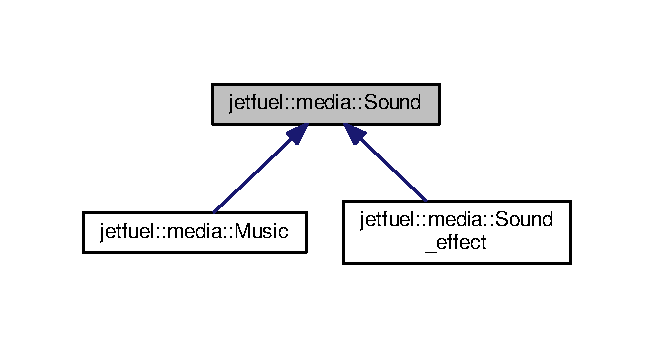
\includegraphics[width=314pt]{classjetfuel_1_1media_1_1Sound__inherit__graph}
\end{center}
\end{figure}
\subsection*{Public Member Functions}
\begin{DoxyCompactItemize}
\item 
virtual \hyperlink{classjetfuel_1_1media_1_1Sound_a9b588c3a8749ce496f19cf499e5d98bb}{$\sim$\+Sound} ()
\begin{DoxyCompactList}\small\item\em Virtual destructor. \end{DoxyCompactList}\item 
virtual bool \hyperlink{classjetfuel_1_1media_1_1Sound_ab18ff9b8dd2001fa11b17649a6a3defb}{Load\+\_\+audio\+\_\+file} (const std\+::string musicfilepath)=0
\begin{DoxyCompactList}\small\item\em Loads an audio file. \end{DoxyCompactList}\item 
virtual void \hyperlink{classjetfuel_1_1media_1_1Sound_a4dec23a59c74ddbdf10386205e68cb29}{Set\+\_\+global\+\_\+volume} (const unsigned int channel, const int volume)
\begin{DoxyCompactList}\small\item\em Sets the G\+L\+O\+B\+A\+L(affects A\+L\+L sound objects) volume. \end{DoxyCompactList}\item 
int \hyperlink{classjetfuel_1_1media_1_1Sound_adf11e3f1005cbad8ffe746e83978200d}{Get\+\_\+frequency} () const
\begin{DoxyCompactList}\small\item\em Gets the current audio frequency(44100 by default). \end{DoxyCompactList}\item 
void \hyperlink{classjetfuel_1_1media_1_1Sound_af67e7d4f9d1509b1a8dcea3e3a7860c8}{Set\+\_\+frequency} (const int frequency)
\begin{DoxyCompactList}\small\item\em Sets the current audio frequency. \end{DoxyCompactList}\item 
Uint16 \hyperlink{classjetfuel_1_1media_1_1Sound_a91d355730fe004228942d38b2e2264b9}{Get\+\_\+format} () const
\begin{DoxyCompactList}\small\item\em Gets the current audio frequency( M\+I\+X\+\_\+\+D\+E\+F\+A\+U\+L\+T\+\_\+\+F\+O\+R\+M\+AT by default). \end{DoxyCompactList}\item 
void \hyperlink{classjetfuel_1_1media_1_1Sound_ac764c3156841b6bd2970d912292ac1ca}{Set\+\_\+format} (Uint16 format)
\begin{DoxyCompactList}\small\item\em Sets the current audio format. \end{DoxyCompactList}\item 
int \hyperlink{classjetfuel_1_1media_1_1Sound_a8f1cbbaaf31a106938968f256e77bad7}{Get\+\_\+chunk\+\_\+size} () const
\begin{DoxyCompactList}\small\item\em Gets the current audio chunk size( 2048 by default). \end{DoxyCompactList}\item 
void \hyperlink{classjetfuel_1_1media_1_1Sound_ad84439e1a101e298b2e5186851ebe0d3}{Set\+\_\+chunk\+\_\+size} (const int chunksize)
\begin{DoxyCompactList}\small\item\em Sets the current audio chunk size. \end{DoxyCompactList}\item 
unsigned int \hyperlink{classjetfuel_1_1media_1_1Sound_a0fe4e0c72224935e14a5481435e855af}{Get\+\_\+number\+\_\+of\+\_\+channels} () const
\begin{DoxyCompactList}\small\item\em Gets the number of audio channels(2 by default). \end{DoxyCompactList}\item 
void \hyperlink{classjetfuel_1_1media_1_1Sound_ac0bb67c175f71ab5977af3f5781cedd7}{Set\+\_\+number\+\_\+of\+\_\+channels} (const unsigned int numofchannels)
\begin{DoxyCompactList}\small\item\em Sets the number of audio channels. \end{DoxyCompactList}\item 
int \hyperlink{classjetfuel_1_1media_1_1Sound_afcef9fca1204403d6f3d52fc4b494463}{Get\+\_\+active\+\_\+channel\+\_\+num} () const
\begin{DoxyCompactList}\small\item\em Gets the current active channel number(-\/1(or automatically choose active channel) by default). \end{DoxyCompactList}\item 
void \hyperlink{classjetfuel_1_1media_1_1Sound_addaea461cf050aa23501882b2c76b39b}{Set\+\_\+active\+\_\+channel\+\_\+num} (const int activechannelnum)
\begin{DoxyCompactList}\small\item\em Sets the current active channel number. \end{DoxyCompactList}\item 
virtual bool \hyperlink{classjetfuel_1_1media_1_1Sound_a8861a6671ce039522179d61085f240c8}{Play} ()=0
\begin{DoxyCompactList}\small\item\em Starts audio playback. \end{DoxyCompactList}\item 
virtual void \hyperlink{classjetfuel_1_1media_1_1Sound_adb9cd45e23e6224760051e579aeefa7f}{Pause} ()=0
\begin{DoxyCompactList}\small\item\em Pauses audio playback. \end{DoxyCompactList}\item 
virtual void \hyperlink{classjetfuel_1_1media_1_1Sound_af781fccd8ebb1305e97dc8f6b7c828dc}{Resume} ()=0
\begin{DoxyCompactList}\small\item\em Resumes audio playback. \end{DoxyCompactList}\end{DoxyCompactItemize}


\subsection{Detailed Description}
A simple base \hyperlink{classjetfuel_1_1media_1_1Sound}{Sound} class that, when inherited, simplifies the process of building an audio playback class significantly.

\begin{DoxySeeAlso}{See also}
\hyperlink{classjetfuel_1_1media_1_1Sound__effect}{jetfuel\+::media\+::\+Sound\+\_\+effect} 

\hyperlink{classjetfuel_1_1media_1_1Music}{jetfuel\+::media\+::\+Music} 
\end{DoxySeeAlso}


\subsection{Constructor \& Destructor Documentation}
\mbox{\Hypertarget{classjetfuel_1_1media_1_1Sound_a9b588c3a8749ce496f19cf499e5d98bb}\label{classjetfuel_1_1media_1_1Sound_a9b588c3a8749ce496f19cf499e5d98bb}} 
\index{jetfuel\+::media\+::\+Sound@{jetfuel\+::media\+::\+Sound}!````~Sound@{$\sim$\+Sound}}
\index{````~Sound@{$\sim$\+Sound}!jetfuel\+::media\+::\+Sound@{jetfuel\+::media\+::\+Sound}}
\subsubsection{\texorpdfstring{$\sim$\+Sound()}{~Sound()}}
{\footnotesize\ttfamily virtual jetfuel\+::media\+::\+Sound\+::$\sim$\+Sound (\begin{DoxyParamCaption}{ }\end{DoxyParamCaption})\hspace{0.3cm}{\ttfamily [inline]}, {\ttfamily [virtual]}}



Virtual destructor. 

Virtual destructor. 

\subsection{Member Function Documentation}
\mbox{\Hypertarget{classjetfuel_1_1media_1_1Sound_afcef9fca1204403d6f3d52fc4b494463}\label{classjetfuel_1_1media_1_1Sound_afcef9fca1204403d6f3d52fc4b494463}} 
\index{jetfuel\+::media\+::\+Sound@{jetfuel\+::media\+::\+Sound}!Get\+\_\+active\+\_\+channel\+\_\+num@{Get\+\_\+active\+\_\+channel\+\_\+num}}
\index{Get\+\_\+active\+\_\+channel\+\_\+num@{Get\+\_\+active\+\_\+channel\+\_\+num}!jetfuel\+::media\+::\+Sound@{jetfuel\+::media\+::\+Sound}}
\subsubsection{\texorpdfstring{Get\+\_\+active\+\_\+channel\+\_\+num()}{Get\_active\_channel\_num()}}
{\footnotesize\ttfamily int jetfuel\+::media\+::\+Sound\+::\+Get\+\_\+active\+\_\+channel\+\_\+num (\begin{DoxyParamCaption}{ }\end{DoxyParamCaption}) const\hspace{0.3cm}{\ttfamily [inline]}}



Gets the current active channel number(-\/1(or automatically choose active channel) by default). 

Gets the current active channel number(-\/1(or automatically choose active channel) by default). \mbox{\Hypertarget{classjetfuel_1_1media_1_1Sound_a8f1cbbaaf31a106938968f256e77bad7}\label{classjetfuel_1_1media_1_1Sound_a8f1cbbaaf31a106938968f256e77bad7}} 
\index{jetfuel\+::media\+::\+Sound@{jetfuel\+::media\+::\+Sound}!Get\+\_\+chunk\+\_\+size@{Get\+\_\+chunk\+\_\+size}}
\index{Get\+\_\+chunk\+\_\+size@{Get\+\_\+chunk\+\_\+size}!jetfuel\+::media\+::\+Sound@{jetfuel\+::media\+::\+Sound}}
\subsubsection{\texorpdfstring{Get\+\_\+chunk\+\_\+size()}{Get\_chunk\_size()}}
{\footnotesize\ttfamily int jetfuel\+::media\+::\+Sound\+::\+Get\+\_\+chunk\+\_\+size (\begin{DoxyParamCaption}{ }\end{DoxyParamCaption}) const\hspace{0.3cm}{\ttfamily [inline]}}



Gets the current audio chunk size( 2048 by default). 

Gets the current audio frequency(2048 by default). \mbox{\Hypertarget{classjetfuel_1_1media_1_1Sound_a91d355730fe004228942d38b2e2264b9}\label{classjetfuel_1_1media_1_1Sound_a91d355730fe004228942d38b2e2264b9}} 
\index{jetfuel\+::media\+::\+Sound@{jetfuel\+::media\+::\+Sound}!Get\+\_\+format@{Get\+\_\+format}}
\index{Get\+\_\+format@{Get\+\_\+format}!jetfuel\+::media\+::\+Sound@{jetfuel\+::media\+::\+Sound}}
\subsubsection{\texorpdfstring{Get\+\_\+format()}{Get\_format()}}
{\footnotesize\ttfamily Uint16 jetfuel\+::media\+::\+Sound\+::\+Get\+\_\+format (\begin{DoxyParamCaption}{ }\end{DoxyParamCaption}) const\hspace{0.3cm}{\ttfamily [inline]}}



Gets the current audio frequency( M\+I\+X\+\_\+\+D\+E\+F\+A\+U\+L\+T\+\_\+\+F\+O\+R\+M\+AT by default). 

Gets the current audio frequency(M\+I\+X\+\_\+\+D\+E\+F\+A\+U\+L\+T\+\_\+\+F\+O\+R\+M\+AT by default). \mbox{\Hypertarget{classjetfuel_1_1media_1_1Sound_adf11e3f1005cbad8ffe746e83978200d}\label{classjetfuel_1_1media_1_1Sound_adf11e3f1005cbad8ffe746e83978200d}} 
\index{jetfuel\+::media\+::\+Sound@{jetfuel\+::media\+::\+Sound}!Get\+\_\+frequency@{Get\+\_\+frequency}}
\index{Get\+\_\+frequency@{Get\+\_\+frequency}!jetfuel\+::media\+::\+Sound@{jetfuel\+::media\+::\+Sound}}
\subsubsection{\texorpdfstring{Get\+\_\+frequency()}{Get\_frequency()}}
{\footnotesize\ttfamily int jetfuel\+::media\+::\+Sound\+::\+Get\+\_\+frequency (\begin{DoxyParamCaption}{ }\end{DoxyParamCaption}) const\hspace{0.3cm}{\ttfamily [inline]}}



Gets the current audio frequency(44100 by default). 

Gets the current audio frequency(44100 by default). \mbox{\Hypertarget{classjetfuel_1_1media_1_1Sound_a0fe4e0c72224935e14a5481435e855af}\label{classjetfuel_1_1media_1_1Sound_a0fe4e0c72224935e14a5481435e855af}} 
\index{jetfuel\+::media\+::\+Sound@{jetfuel\+::media\+::\+Sound}!Get\+\_\+number\+\_\+of\+\_\+channels@{Get\+\_\+number\+\_\+of\+\_\+channels}}
\index{Get\+\_\+number\+\_\+of\+\_\+channels@{Get\+\_\+number\+\_\+of\+\_\+channels}!jetfuel\+::media\+::\+Sound@{jetfuel\+::media\+::\+Sound}}
\subsubsection{\texorpdfstring{Get\+\_\+number\+\_\+of\+\_\+channels()}{Get\_number\_of\_channels()}}
{\footnotesize\ttfamily unsigned int jetfuel\+::media\+::\+Sound\+::\+Get\+\_\+number\+\_\+of\+\_\+channels (\begin{DoxyParamCaption}{ }\end{DoxyParamCaption}) const\hspace{0.3cm}{\ttfamily [inline]}}



Gets the number of audio channels(2 by default). 

Gets the number of audio channels(2 by default). \mbox{\Hypertarget{classjetfuel_1_1media_1_1Sound_ab18ff9b8dd2001fa11b17649a6a3defb}\label{classjetfuel_1_1media_1_1Sound_ab18ff9b8dd2001fa11b17649a6a3defb}} 
\index{jetfuel\+::media\+::\+Sound@{jetfuel\+::media\+::\+Sound}!Load\+\_\+audio\+\_\+file@{Load\+\_\+audio\+\_\+file}}
\index{Load\+\_\+audio\+\_\+file@{Load\+\_\+audio\+\_\+file}!jetfuel\+::media\+::\+Sound@{jetfuel\+::media\+::\+Sound}}
\subsubsection{\texorpdfstring{Load\+\_\+audio\+\_\+file()}{Load\_audio\_file()}}
{\footnotesize\ttfamily virtual bool jetfuel\+::media\+::\+Sound\+::\+Load\+\_\+audio\+\_\+file (\begin{DoxyParamCaption}\item[{const std\+::string}]{musicfilepath }\end{DoxyParamCaption})\hspace{0.3cm}{\ttfamily [pure virtual]}}



Loads an audio file. 

Loads an audio file. This is a pure virtual function that any children M\+U\+ST implement.


\begin{DoxyParams}{Parameters}
{\em std\+::string} & musicfilepath \\
\hline
\end{DoxyParams}


Implemented in \hyperlink{classjetfuel_1_1media_1_1Music_ae24079b0301f5cf845d094e32ed22da1}{jetfuel\+::media\+::\+Music}, and \hyperlink{classjetfuel_1_1media_1_1Sound__effect_a1ad701cd2318e960bde2ab063aeabb75}{jetfuel\+::media\+::\+Sound\+\_\+effect}.

\mbox{\Hypertarget{classjetfuel_1_1media_1_1Sound_adb9cd45e23e6224760051e579aeefa7f}\label{classjetfuel_1_1media_1_1Sound_adb9cd45e23e6224760051e579aeefa7f}} 
\index{jetfuel\+::media\+::\+Sound@{jetfuel\+::media\+::\+Sound}!Pause@{Pause}}
\index{Pause@{Pause}!jetfuel\+::media\+::\+Sound@{jetfuel\+::media\+::\+Sound}}
\subsubsection{\texorpdfstring{Pause()}{Pause()}}
{\footnotesize\ttfamily virtual void jetfuel\+::media\+::\+Sound\+::\+Pause (\begin{DoxyParamCaption}{ }\end{DoxyParamCaption})\hspace{0.3cm}{\ttfamily [pure virtual]}}



Pauses audio playback. 

Pauses audio playback. This is a pure virtual function that any children M\+U\+ST implement. 

Implemented in \hyperlink{classjetfuel_1_1media_1_1Sound__effect_a5fa5bb67a349bac545f233a6aa8a030d}{jetfuel\+::media\+::\+Sound\+\_\+effect}, and \hyperlink{classjetfuel_1_1media_1_1Music_a002f31a60671c229bd054539caf537c5}{jetfuel\+::media\+::\+Music}.

\mbox{\Hypertarget{classjetfuel_1_1media_1_1Sound_a8861a6671ce039522179d61085f240c8}\label{classjetfuel_1_1media_1_1Sound_a8861a6671ce039522179d61085f240c8}} 
\index{jetfuel\+::media\+::\+Sound@{jetfuel\+::media\+::\+Sound}!Play@{Play}}
\index{Play@{Play}!jetfuel\+::media\+::\+Sound@{jetfuel\+::media\+::\+Sound}}
\subsubsection{\texorpdfstring{Play()}{Play()}}
{\footnotesize\ttfamily virtual bool jetfuel\+::media\+::\+Sound\+::\+Play (\begin{DoxyParamCaption}{ }\end{DoxyParamCaption})\hspace{0.3cm}{\ttfamily [pure virtual]}}



Starts audio playback. 

Starts audio playback. This is a pure virtual function that any children M\+U\+ST implement. 

Implemented in \hyperlink{classjetfuel_1_1media_1_1Sound__effect_a206d3653259cc854fd80fa44a9d333c4}{jetfuel\+::media\+::\+Sound\+\_\+effect}, and \hyperlink{classjetfuel_1_1media_1_1Music_afe9abee662a68ea9391e94e37c79945e}{jetfuel\+::media\+::\+Music}.

\mbox{\Hypertarget{classjetfuel_1_1media_1_1Sound_af781fccd8ebb1305e97dc8f6b7c828dc}\label{classjetfuel_1_1media_1_1Sound_af781fccd8ebb1305e97dc8f6b7c828dc}} 
\index{jetfuel\+::media\+::\+Sound@{jetfuel\+::media\+::\+Sound}!Resume@{Resume}}
\index{Resume@{Resume}!jetfuel\+::media\+::\+Sound@{jetfuel\+::media\+::\+Sound}}
\subsubsection{\texorpdfstring{Resume()}{Resume()}}
{\footnotesize\ttfamily virtual void jetfuel\+::media\+::\+Sound\+::\+Resume (\begin{DoxyParamCaption}{ }\end{DoxyParamCaption})\hspace{0.3cm}{\ttfamily [pure virtual]}}



Resumes audio playback. 

Resumes audio playback. This is a pure virtual function that any children M\+U\+ST implement. 

Implemented in \hyperlink{classjetfuel_1_1media_1_1Sound__effect_a8849f5324b2c049c63ed3a0bbbd88467}{jetfuel\+::media\+::\+Sound\+\_\+effect}, and \hyperlink{classjetfuel_1_1media_1_1Music_a0c8e12634e29cfe37138349776b6d9a8}{jetfuel\+::media\+::\+Music}.

\mbox{\Hypertarget{classjetfuel_1_1media_1_1Sound_addaea461cf050aa23501882b2c76b39b}\label{classjetfuel_1_1media_1_1Sound_addaea461cf050aa23501882b2c76b39b}} 
\index{jetfuel\+::media\+::\+Sound@{jetfuel\+::media\+::\+Sound}!Set\+\_\+active\+\_\+channel\+\_\+num@{Set\+\_\+active\+\_\+channel\+\_\+num}}
\index{Set\+\_\+active\+\_\+channel\+\_\+num@{Set\+\_\+active\+\_\+channel\+\_\+num}!jetfuel\+::media\+::\+Sound@{jetfuel\+::media\+::\+Sound}}
\subsubsection{\texorpdfstring{Set\+\_\+active\+\_\+channel\+\_\+num()}{Set\_active\_channel\_num()}}
{\footnotesize\ttfamily void jetfuel\+::media\+::\+Sound\+::\+Set\+\_\+active\+\_\+channel\+\_\+num (\begin{DoxyParamCaption}\item[{const int}]{activechannelnum }\end{DoxyParamCaption})\hspace{0.3cm}{\ttfamily [inline]}}



Sets the current active channel number. 

Sets the current active channel number. At the risk of sounding obvious\+: Don\textquotesingle{}t mess with this unless you know what you are doing.


\begin{DoxyParams}{Parameters}
{\em int} & activechannelnum \\
\hline
\end{DoxyParams}
\mbox{\Hypertarget{classjetfuel_1_1media_1_1Sound_ad84439e1a101e298b2e5186851ebe0d3}\label{classjetfuel_1_1media_1_1Sound_ad84439e1a101e298b2e5186851ebe0d3}} 
\index{jetfuel\+::media\+::\+Sound@{jetfuel\+::media\+::\+Sound}!Set\+\_\+chunk\+\_\+size@{Set\+\_\+chunk\+\_\+size}}
\index{Set\+\_\+chunk\+\_\+size@{Set\+\_\+chunk\+\_\+size}!jetfuel\+::media\+::\+Sound@{jetfuel\+::media\+::\+Sound}}
\subsubsection{\texorpdfstring{Set\+\_\+chunk\+\_\+size()}{Set\_chunk\_size()}}
{\footnotesize\ttfamily void jetfuel\+::media\+::\+Sound\+::\+Set\+\_\+chunk\+\_\+size (\begin{DoxyParamCaption}\item[{const int}]{chunksize }\end{DoxyParamCaption})\hspace{0.3cm}{\ttfamily [inline]}}



Sets the current audio chunk size. 

Sets the current audio chunk size. At the risk of sounding obvious\+: Don\textquotesingle{}t mess with this unless you know what you are doing.


\begin{DoxyParams}{Parameters}
{\em int} & chunksize \\
\hline
\end{DoxyParams}
\mbox{\Hypertarget{classjetfuel_1_1media_1_1Sound_ac764c3156841b6bd2970d912292ac1ca}\label{classjetfuel_1_1media_1_1Sound_ac764c3156841b6bd2970d912292ac1ca}} 
\index{jetfuel\+::media\+::\+Sound@{jetfuel\+::media\+::\+Sound}!Set\+\_\+format@{Set\+\_\+format}}
\index{Set\+\_\+format@{Set\+\_\+format}!jetfuel\+::media\+::\+Sound@{jetfuel\+::media\+::\+Sound}}
\subsubsection{\texorpdfstring{Set\+\_\+format()}{Set\_format()}}
{\footnotesize\ttfamily void jetfuel\+::media\+::\+Sound\+::\+Set\+\_\+format (\begin{DoxyParamCaption}\item[{Uint16}]{format }\end{DoxyParamCaption})\hspace{0.3cm}{\ttfamily [inline]}}



Sets the current audio format. 

Sets the current audio format. At the risk of sounding obvious\+: Don\textquotesingle{}t mess with this unless you know what you are doing.


\begin{DoxyParams}{Parameters}
{\em Uint16} & format \\
\hline
\end{DoxyParams}
\mbox{\Hypertarget{classjetfuel_1_1media_1_1Sound_af67e7d4f9d1509b1a8dcea3e3a7860c8}\label{classjetfuel_1_1media_1_1Sound_af67e7d4f9d1509b1a8dcea3e3a7860c8}} 
\index{jetfuel\+::media\+::\+Sound@{jetfuel\+::media\+::\+Sound}!Set\+\_\+frequency@{Set\+\_\+frequency}}
\index{Set\+\_\+frequency@{Set\+\_\+frequency}!jetfuel\+::media\+::\+Sound@{jetfuel\+::media\+::\+Sound}}
\subsubsection{\texorpdfstring{Set\+\_\+frequency()}{Set\_frequency()}}
{\footnotesize\ttfamily void jetfuel\+::media\+::\+Sound\+::\+Set\+\_\+frequency (\begin{DoxyParamCaption}\item[{const int}]{frequency }\end{DoxyParamCaption})\hspace{0.3cm}{\ttfamily [inline]}}



Sets the current audio frequency. 

Sets the current audio frequency. At the risk of sounding obvious\+: Don\textquotesingle{}t mess with this unless you know what you are doing.


\begin{DoxyParams}{Parameters}
{\em int} & frequency \\
\hline
\end{DoxyParams}
\mbox{\Hypertarget{classjetfuel_1_1media_1_1Sound_a4dec23a59c74ddbdf10386205e68cb29}\label{classjetfuel_1_1media_1_1Sound_a4dec23a59c74ddbdf10386205e68cb29}} 
\index{jetfuel\+::media\+::\+Sound@{jetfuel\+::media\+::\+Sound}!Set\+\_\+global\+\_\+volume@{Set\+\_\+global\+\_\+volume}}
\index{Set\+\_\+global\+\_\+volume@{Set\+\_\+global\+\_\+volume}!jetfuel\+::media\+::\+Sound@{jetfuel\+::media\+::\+Sound}}
\subsubsection{\texorpdfstring{Set\+\_\+global\+\_\+volume()}{Set\_global\_volume()}}
{\footnotesize\ttfamily virtual void jetfuel\+::media\+::\+Sound\+::\+Set\+\_\+global\+\_\+volume (\begin{DoxyParamCaption}\item[{const unsigned int}]{channel,  }\item[{const int}]{volume }\end{DoxyParamCaption})\hspace{0.3cm}{\ttfamily [inline]}, {\ttfamily [virtual]}}



Sets the G\+L\+O\+B\+A\+L(affects A\+L\+L sound objects) volume. 

Sets the G\+L\+O\+B\+A\+L(affects A\+L\+L sound objects) volume.


\begin{DoxyParams}{Parameters}
{\em unsigned} & int channel \\
\hline
{\em int} & volume \\
\hline
\end{DoxyParams}
\mbox{\Hypertarget{classjetfuel_1_1media_1_1Sound_ac0bb67c175f71ab5977af3f5781cedd7}\label{classjetfuel_1_1media_1_1Sound_ac0bb67c175f71ab5977af3f5781cedd7}} 
\index{jetfuel\+::media\+::\+Sound@{jetfuel\+::media\+::\+Sound}!Set\+\_\+number\+\_\+of\+\_\+channels@{Set\+\_\+number\+\_\+of\+\_\+channels}}
\index{Set\+\_\+number\+\_\+of\+\_\+channels@{Set\+\_\+number\+\_\+of\+\_\+channels}!jetfuel\+::media\+::\+Sound@{jetfuel\+::media\+::\+Sound}}
\subsubsection{\texorpdfstring{Set\+\_\+number\+\_\+of\+\_\+channels()}{Set\_number\_of\_channels()}}
{\footnotesize\ttfamily void jetfuel\+::media\+::\+Sound\+::\+Set\+\_\+number\+\_\+of\+\_\+channels (\begin{DoxyParamCaption}\item[{const unsigned int}]{numofchannels }\end{DoxyParamCaption})\hspace{0.3cm}{\ttfamily [inline]}}



Sets the number of audio channels. 

Sets the number of audio channels.


\begin{DoxyParams}{Parameters}
{\em unsigned} & int numofchannels \\
\hline
\end{DoxyParams}


The documentation for this class was generated from the following file\+:\begin{DoxyCompactItemize}
\item 
include/jetfuelmedia/sound.\+h\end{DoxyCompactItemize}

\hypertarget{classjetfuel_1_1media_1_1Sound__effect}{}\section{jetfuel\+:\+:media\+:\+:Sound\+\_\+effect Class Reference}
\label{classjetfuel_1_1media_1_1Sound__effect}\index{jetfuel\+::media\+::\+Sound\+\_\+effect@{jetfuel\+::media\+::\+Sound\+\_\+effect}}


{\ttfamily \#include $<$soundeffect.\+h$>$}



Inheritance diagram for jetfuel\+:\+:media\+:\+:Sound\+\_\+effect\+:
\nopagebreak
\begin{figure}[H]
\begin{center}
\leavevmode
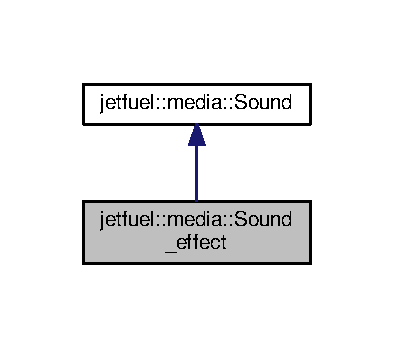
\includegraphics[width=189pt]{classjetfuel_1_1media_1_1Sound__effect__inherit__graph}
\end{center}
\end{figure}


Collaboration diagram for jetfuel\+:\+:media\+:\+:Sound\+\_\+effect\+:
\nopagebreak
\begin{figure}[H]
\begin{center}
\leavevmode
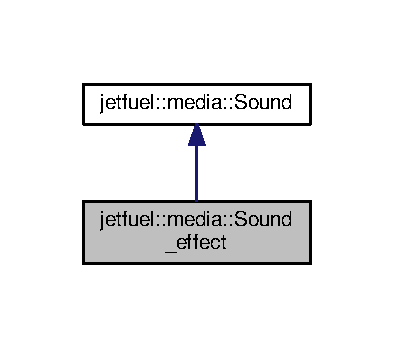
\includegraphics[width=189pt]{classjetfuel_1_1media_1_1Sound__effect__coll__graph}
\end{center}
\end{figure}
\subsection*{Public Member Functions}
\begin{DoxyCompactItemize}
\item 
\hyperlink{classjetfuel_1_1media_1_1Sound__effect_a56c5c69d077a4cac1a062b391a9860fc}{Sound\+\_\+effect} ()
\begin{DoxyCompactList}\small\item\em Default constructor. \end{DoxyCompactList}\item 
virtual \hyperlink{classjetfuel_1_1media_1_1Sound__effect_a105547b1d854a256e90a08fcd6098bdf}{$\sim$\+Sound\+\_\+effect} ()
\begin{DoxyCompactList}\small\item\em Virtual destructor. \end{DoxyCompactList}\item 
std\+::string \hyperlink{classjetfuel_1_1media_1_1Sound__effect_ab172a8c2a1057970e343dfe81aeb208f}{Get\+\_\+loaded\+\_\+audio\+\_\+file\+\_\+path} () const
\begin{DoxyCompactList}\small\item\em Gets the loaded audio\textquotesingle{}s file path. \end{DoxyCompactList}\item 
bool \hyperlink{classjetfuel_1_1media_1_1Sound__effect_a1ad701cd2318e960bde2ab063aeabb75}{Load\+\_\+audio\+\_\+file} (const std\+::string musicfilepath) override
\begin{DoxyCompactList}\small\item\em Loads a sound effect file from a given file path. \end{DoxyCompactList}\item 
unsigned int \hyperlink{classjetfuel_1_1media_1_1Sound__effect_aa0fcc463543949dfe45efb41b8df93db}{Get\+\_\+times\+\_\+to\+\_\+repeat} () const
\begin{DoxyCompactList}\small\item\em Gets the times to repeat this \hyperlink{classjetfuel_1_1media_1_1Sound__effect}{Sound\+\_\+effect}. \end{DoxyCompactList}\item 
void \hyperlink{classjetfuel_1_1media_1_1Sound__effect_a79c40daad35fcce6cd7553747273f457}{Set\+\_\+times\+\_\+to\+\_\+repeat} (const unsigned int repeattimes)
\begin{DoxyCompactList}\small\item\em Sets the times to repeat this \hyperlink{classjetfuel_1_1media_1_1Sound__effect}{Sound\+\_\+effect}. \end{DoxyCompactList}\item 
bool \hyperlink{classjetfuel_1_1media_1_1Sound__effect_a206d3653259cc854fd80fa44a9d333c4}{Play} () override
\begin{DoxyCompactList}\small\item\em Plays this \hyperlink{classjetfuel_1_1media_1_1Sound__effect}{Sound\+\_\+effect}. \end{DoxyCompactList}\item 
void \hyperlink{classjetfuel_1_1media_1_1Sound__effect_a5fa5bb67a349bac545f233a6aa8a030d}{Pause} () override
\begin{DoxyCompactList}\small\item\em Pauses this \hyperlink{classjetfuel_1_1media_1_1Sound__effect}{Sound\+\_\+effect}. \end{DoxyCompactList}\item 
void \hyperlink{classjetfuel_1_1media_1_1Sound__effect_a8849f5324b2c049c63ed3a0bbbd88467}{Resume} () override
\begin{DoxyCompactList}\small\item\em Resumes this \hyperlink{classjetfuel_1_1media_1_1Sound__effect}{Sound\+\_\+effect}. \end{DoxyCompactList}\end{DoxyCompactItemize}
\subsection*{Static Public Member Functions}
\begin{DoxyCompactItemize}
\item 
static bool \hyperlink{classjetfuel_1_1media_1_1Sound__effect_ae81630f796281931d9c2f1dc3a0e9319}{Is\+\_\+sound\+\_\+effect\+\_\+or\+\_\+music\+\_\+playing} ()
\begin{DoxyCompactList}\small\item\em Returns whether A\+NY sound is playing. \end{DoxyCompactList}\end{DoxyCompactItemize}
\subsection*{Protected Member Functions}
\begin{DoxyCompactItemize}
\item 
bool \hyperlink{classjetfuel_1_1media_1_1Sound__effect_a6f646b304bc3617e027a4d503e4124db}{Is\+\_\+sound\+\_\+effect\+\_\+loaded} () const
\begin{DoxyCompactList}\small\item\em Returns whether this \hyperlink{classjetfuel_1_1media_1_1Sound__effect}{Sound\+\_\+effect} is loaded. \end{DoxyCompactList}\item 
bool \hyperlink{classjetfuel_1_1media_1_1Sound__effect_abb1c6c0b2eba2d167b654af7cbcd6d24}{Play\+\_\+sound\+\_\+effect} ()
\begin{DoxyCompactList}\small\item\em Plays this \hyperlink{classjetfuel_1_1media_1_1Sound__effect}{Sound\+\_\+effect} using S\+D\+L\+\_\+mixer. \end{DoxyCompactList}\item 
void \hyperlink{classjetfuel_1_1media_1_1Sound__effect_a76b2b58d4ca2c1fe9988a4cdc4f96a3d}{Pause\+\_\+sound\+\_\+effect} ()
\begin{DoxyCompactList}\small\item\em Pauses this \hyperlink{classjetfuel_1_1media_1_1Sound__effect}{Sound\+\_\+effect} using S\+D\+L\+\_\+mixer. \end{DoxyCompactList}\item 
void \hyperlink{classjetfuel_1_1media_1_1Sound__effect_aa810e2cf5bd4f147b81755690c96f203}{Resume\+\_\+sound\+\_\+effect} ()
\begin{DoxyCompactList}\small\item\em Resumes this \hyperlink{classjetfuel_1_1media_1_1Sound__effect}{Sound\+\_\+effect} using S\+D\+L\+\_\+mixer. \end{DoxyCompactList}\end{DoxyCompactItemize}


\subsection{Detailed Description}
A sound playback class for short(and sweet) audio files, which supports W\+AV(.wav), A\+I\+FF(.aiff), V\+OC(.voc), M\+OD(.mod, .xm, .s3m, and more), M\+I\+DI(.mid), Ogg\+Vorbis(.ogg), M\+P3(.mp3), and F\+L\+AC(.flac).

Code Example\+:

\hyperlink{classjetfuel_1_1media_1_1Sound__effect}{jetfuel\+::media\+::\+Sound\+\_\+effect} sfx;

if(sfx.\+load\+\_\+audio\+\_\+file(\char`\"{}\+S\+F\+X.\+ogg\char`\"{}))\{ std\+::cout $<$$<$ \char`\"{}\+Unable to load S\+F\+X.\+ogg Error\+:\char`\"{} $<$$<$ Mix\+\_\+\+Get\+Error() $<$$<$ std\+:endl; return 1; \}

sfx.\+Play(); 

\subsection{Constructor \& Destructor Documentation}
\mbox{\Hypertarget{classjetfuel_1_1media_1_1Sound__effect_a56c5c69d077a4cac1a062b391a9860fc}\label{classjetfuel_1_1media_1_1Sound__effect_a56c5c69d077a4cac1a062b391a9860fc}} 
\index{jetfuel\+::media\+::\+Sound\+\_\+effect@{jetfuel\+::media\+::\+Sound\+\_\+effect}!Sound\+\_\+effect@{Sound\+\_\+effect}}
\index{Sound\+\_\+effect@{Sound\+\_\+effect}!jetfuel\+::media\+::\+Sound\+\_\+effect@{jetfuel\+::media\+::\+Sound\+\_\+effect}}
\subsubsection{\texorpdfstring{Sound\+\_\+effect()}{Sound\_effect()}}
{\footnotesize\ttfamily jetfuel\+::media\+::\+Sound\+\_\+effect\+::\+Sound\+\_\+effect (\begin{DoxyParamCaption}{ }\end{DoxyParamCaption})}



Default constructor. 

Default constructor. \mbox{\Hypertarget{classjetfuel_1_1media_1_1Sound__effect_a105547b1d854a256e90a08fcd6098bdf}\label{classjetfuel_1_1media_1_1Sound__effect_a105547b1d854a256e90a08fcd6098bdf}} 
\index{jetfuel\+::media\+::\+Sound\+\_\+effect@{jetfuel\+::media\+::\+Sound\+\_\+effect}!````~Sound\+\_\+effect@{$\sim$\+Sound\+\_\+effect}}
\index{````~Sound\+\_\+effect@{$\sim$\+Sound\+\_\+effect}!jetfuel\+::media\+::\+Sound\+\_\+effect@{jetfuel\+::media\+::\+Sound\+\_\+effect}}
\subsubsection{\texorpdfstring{$\sim$\+Sound\+\_\+effect()}{~Sound\_effect()}}
{\footnotesize\ttfamily virtual jetfuel\+::media\+::\+Sound\+\_\+effect\+::$\sim$\+Sound\+\_\+effect (\begin{DoxyParamCaption}{ }\end{DoxyParamCaption})\hspace{0.3cm}{\ttfamily [virtual]}}



Virtual destructor. 

Virtual destructor. 

\subsection{Member Function Documentation}
\mbox{\Hypertarget{classjetfuel_1_1media_1_1Sound__effect_ab172a8c2a1057970e343dfe81aeb208f}\label{classjetfuel_1_1media_1_1Sound__effect_ab172a8c2a1057970e343dfe81aeb208f}} 
\index{jetfuel\+::media\+::\+Sound\+\_\+effect@{jetfuel\+::media\+::\+Sound\+\_\+effect}!Get\+\_\+loaded\+\_\+audio\+\_\+file\+\_\+path@{Get\+\_\+loaded\+\_\+audio\+\_\+file\+\_\+path}}
\index{Get\+\_\+loaded\+\_\+audio\+\_\+file\+\_\+path@{Get\+\_\+loaded\+\_\+audio\+\_\+file\+\_\+path}!jetfuel\+::media\+::\+Sound\+\_\+effect@{jetfuel\+::media\+::\+Sound\+\_\+effect}}
\subsubsection{\texorpdfstring{Get\+\_\+loaded\+\_\+audio\+\_\+file\+\_\+path()}{Get\_loaded\_audio\_file\_path()}}
{\footnotesize\ttfamily std\+::string jetfuel\+::media\+::\+Sound\+\_\+effect\+::\+Get\+\_\+loaded\+\_\+audio\+\_\+file\+\_\+path (\begin{DoxyParamCaption}{ }\end{DoxyParamCaption}) const\hspace{0.3cm}{\ttfamily [inline]}}



Gets the loaded audio\textquotesingle{}s file path. 

Gets the loaded audio\textquotesingle{}s file path. \mbox{\Hypertarget{classjetfuel_1_1media_1_1Sound__effect_aa0fcc463543949dfe45efb41b8df93db}\label{classjetfuel_1_1media_1_1Sound__effect_aa0fcc463543949dfe45efb41b8df93db}} 
\index{jetfuel\+::media\+::\+Sound\+\_\+effect@{jetfuel\+::media\+::\+Sound\+\_\+effect}!Get\+\_\+times\+\_\+to\+\_\+repeat@{Get\+\_\+times\+\_\+to\+\_\+repeat}}
\index{Get\+\_\+times\+\_\+to\+\_\+repeat@{Get\+\_\+times\+\_\+to\+\_\+repeat}!jetfuel\+::media\+::\+Sound\+\_\+effect@{jetfuel\+::media\+::\+Sound\+\_\+effect}}
\subsubsection{\texorpdfstring{Get\+\_\+times\+\_\+to\+\_\+repeat()}{Get\_times\_to\_repeat()}}
{\footnotesize\ttfamily unsigned int jetfuel\+::media\+::\+Sound\+\_\+effect\+::\+Get\+\_\+times\+\_\+to\+\_\+repeat (\begin{DoxyParamCaption}{ }\end{DoxyParamCaption}) const\hspace{0.3cm}{\ttfamily [inline]}}



Gets the times to repeat this \hyperlink{classjetfuel_1_1media_1_1Sound__effect}{Sound\+\_\+effect}. 

Gets the times to repeat this \hyperlink{classjetfuel_1_1media_1_1Sound__effect}{Sound\+\_\+effect}. \mbox{\Hypertarget{classjetfuel_1_1media_1_1Sound__effect_a6f646b304bc3617e027a4d503e4124db}\label{classjetfuel_1_1media_1_1Sound__effect_a6f646b304bc3617e027a4d503e4124db}} 
\index{jetfuel\+::media\+::\+Sound\+\_\+effect@{jetfuel\+::media\+::\+Sound\+\_\+effect}!Is\+\_\+sound\+\_\+effect\+\_\+loaded@{Is\+\_\+sound\+\_\+effect\+\_\+loaded}}
\index{Is\+\_\+sound\+\_\+effect\+\_\+loaded@{Is\+\_\+sound\+\_\+effect\+\_\+loaded}!jetfuel\+::media\+::\+Sound\+\_\+effect@{jetfuel\+::media\+::\+Sound\+\_\+effect}}
\subsubsection{\texorpdfstring{Is\+\_\+sound\+\_\+effect\+\_\+loaded()}{Is\_sound\_effect\_loaded()}}
{\footnotesize\ttfamily bool jetfuel\+::media\+::\+Sound\+\_\+effect\+::\+Is\+\_\+sound\+\_\+effect\+\_\+loaded (\begin{DoxyParamCaption}{ }\end{DoxyParamCaption}) const\hspace{0.3cm}{\ttfamily [inline]}, {\ttfamily [protected]}}



Returns whether this \hyperlink{classjetfuel_1_1media_1_1Sound__effect}{Sound\+\_\+effect} is loaded. 

Returns whether this \hyperlink{classjetfuel_1_1media_1_1Sound__effect}{Sound\+\_\+effect} is loaded. \mbox{\Hypertarget{classjetfuel_1_1media_1_1Sound__effect_ae81630f796281931d9c2f1dc3a0e9319}\label{classjetfuel_1_1media_1_1Sound__effect_ae81630f796281931d9c2f1dc3a0e9319}} 
\index{jetfuel\+::media\+::\+Sound\+\_\+effect@{jetfuel\+::media\+::\+Sound\+\_\+effect}!Is\+\_\+sound\+\_\+effect\+\_\+or\+\_\+music\+\_\+playing@{Is\+\_\+sound\+\_\+effect\+\_\+or\+\_\+music\+\_\+playing}}
\index{Is\+\_\+sound\+\_\+effect\+\_\+or\+\_\+music\+\_\+playing@{Is\+\_\+sound\+\_\+effect\+\_\+or\+\_\+music\+\_\+playing}!jetfuel\+::media\+::\+Sound\+\_\+effect@{jetfuel\+::media\+::\+Sound\+\_\+effect}}
\subsubsection{\texorpdfstring{Is\+\_\+sound\+\_\+effect\+\_\+or\+\_\+music\+\_\+playing()}{Is\_sound\_effect\_or\_music\_playing()}}
{\footnotesize\ttfamily static bool jetfuel\+::media\+::\+Sound\+\_\+effect\+::\+Is\+\_\+sound\+\_\+effect\+\_\+or\+\_\+music\+\_\+playing (\begin{DoxyParamCaption}{ }\end{DoxyParamCaption})\hspace{0.3cm}{\ttfamily [inline]}, {\ttfamily [static]}}



Returns whether A\+NY sound is playing. 

Returns whether A\+NY sound is playing. \mbox{\Hypertarget{classjetfuel_1_1media_1_1Sound__effect_a1ad701cd2318e960bde2ab063aeabb75}\label{classjetfuel_1_1media_1_1Sound__effect_a1ad701cd2318e960bde2ab063aeabb75}} 
\index{jetfuel\+::media\+::\+Sound\+\_\+effect@{jetfuel\+::media\+::\+Sound\+\_\+effect}!Load\+\_\+audio\+\_\+file@{Load\+\_\+audio\+\_\+file}}
\index{Load\+\_\+audio\+\_\+file@{Load\+\_\+audio\+\_\+file}!jetfuel\+::media\+::\+Sound\+\_\+effect@{jetfuel\+::media\+::\+Sound\+\_\+effect}}
\subsubsection{\texorpdfstring{Load\+\_\+audio\+\_\+file()}{Load\_audio\_file()}}
{\footnotesize\ttfamily bool jetfuel\+::media\+::\+Sound\+\_\+effect\+::\+Load\+\_\+audio\+\_\+file (\begin{DoxyParamCaption}\item[{const std\+::string}]{musicfilepath }\end{DoxyParamCaption})\hspace{0.3cm}{\ttfamily [inline]}, {\ttfamily [override]}, {\ttfamily [virtual]}}



Loads a sound effect file from a given file path. 

Loads a sound effect file from a given file path.


\begin{DoxyParams}{Parameters}
{\em std\+::string} & musicfilepath \\
\hline
\end{DoxyParams}


Implements \hyperlink{classjetfuel_1_1media_1_1Sound_ab18ff9b8dd2001fa11b17649a6a3defb}{jetfuel\+::media\+::\+Sound}.

\mbox{\Hypertarget{classjetfuel_1_1media_1_1Sound__effect_a5fa5bb67a349bac545f233a6aa8a030d}\label{classjetfuel_1_1media_1_1Sound__effect_a5fa5bb67a349bac545f233a6aa8a030d}} 
\index{jetfuel\+::media\+::\+Sound\+\_\+effect@{jetfuel\+::media\+::\+Sound\+\_\+effect}!Pause@{Pause}}
\index{Pause@{Pause}!jetfuel\+::media\+::\+Sound\+\_\+effect@{jetfuel\+::media\+::\+Sound\+\_\+effect}}
\subsubsection{\texorpdfstring{Pause()}{Pause()}}
{\footnotesize\ttfamily void jetfuel\+::media\+::\+Sound\+\_\+effect\+::\+Pause (\begin{DoxyParamCaption}{ }\end{DoxyParamCaption})\hspace{0.3cm}{\ttfamily [override]}, {\ttfamily [virtual]}}



Pauses this \hyperlink{classjetfuel_1_1media_1_1Sound__effect}{Sound\+\_\+effect}. 

Pauses this \hyperlink{classjetfuel_1_1media_1_1Sound__effect}{Sound\+\_\+effect}. 

Implements \hyperlink{classjetfuel_1_1media_1_1Sound_adb9cd45e23e6224760051e579aeefa7f}{jetfuel\+::media\+::\+Sound}.

\mbox{\Hypertarget{classjetfuel_1_1media_1_1Sound__effect_a76b2b58d4ca2c1fe9988a4cdc4f96a3d}\label{classjetfuel_1_1media_1_1Sound__effect_a76b2b58d4ca2c1fe9988a4cdc4f96a3d}} 
\index{jetfuel\+::media\+::\+Sound\+\_\+effect@{jetfuel\+::media\+::\+Sound\+\_\+effect}!Pause\+\_\+sound\+\_\+effect@{Pause\+\_\+sound\+\_\+effect}}
\index{Pause\+\_\+sound\+\_\+effect@{Pause\+\_\+sound\+\_\+effect}!jetfuel\+::media\+::\+Sound\+\_\+effect@{jetfuel\+::media\+::\+Sound\+\_\+effect}}
\subsubsection{\texorpdfstring{Pause\+\_\+sound\+\_\+effect()}{Pause\_sound\_effect()}}
{\footnotesize\ttfamily void jetfuel\+::media\+::\+Sound\+\_\+effect\+::\+Pause\+\_\+sound\+\_\+effect (\begin{DoxyParamCaption}{ }\end{DoxyParamCaption})\hspace{0.3cm}{\ttfamily [inline]}, {\ttfamily [protected]}}



Pauses this \hyperlink{classjetfuel_1_1media_1_1Sound__effect}{Sound\+\_\+effect} using S\+D\+L\+\_\+mixer. 

Pauses this \hyperlink{classjetfuel_1_1media_1_1Sound__effect}{Sound\+\_\+effect} using S\+D\+L\+\_\+mixer. \mbox{\Hypertarget{classjetfuel_1_1media_1_1Sound__effect_a206d3653259cc854fd80fa44a9d333c4}\label{classjetfuel_1_1media_1_1Sound__effect_a206d3653259cc854fd80fa44a9d333c4}} 
\index{jetfuel\+::media\+::\+Sound\+\_\+effect@{jetfuel\+::media\+::\+Sound\+\_\+effect}!Play@{Play}}
\index{Play@{Play}!jetfuel\+::media\+::\+Sound\+\_\+effect@{jetfuel\+::media\+::\+Sound\+\_\+effect}}
\subsubsection{\texorpdfstring{Play()}{Play()}}
{\footnotesize\ttfamily bool jetfuel\+::media\+::\+Sound\+\_\+effect\+::\+Play (\begin{DoxyParamCaption}{ }\end{DoxyParamCaption})\hspace{0.3cm}{\ttfamily [override]}, {\ttfamily [virtual]}}



Plays this \hyperlink{classjetfuel_1_1media_1_1Sound__effect}{Sound\+\_\+effect}. 

Plays this \hyperlink{classjetfuel_1_1media_1_1Sound__effect}{Sound\+\_\+effect}. 

Implements \hyperlink{classjetfuel_1_1media_1_1Sound_a8861a6671ce039522179d61085f240c8}{jetfuel\+::media\+::\+Sound}.

\mbox{\Hypertarget{classjetfuel_1_1media_1_1Sound__effect_abb1c6c0b2eba2d167b654af7cbcd6d24}\label{classjetfuel_1_1media_1_1Sound__effect_abb1c6c0b2eba2d167b654af7cbcd6d24}} 
\index{jetfuel\+::media\+::\+Sound\+\_\+effect@{jetfuel\+::media\+::\+Sound\+\_\+effect}!Play\+\_\+sound\+\_\+effect@{Play\+\_\+sound\+\_\+effect}}
\index{Play\+\_\+sound\+\_\+effect@{Play\+\_\+sound\+\_\+effect}!jetfuel\+::media\+::\+Sound\+\_\+effect@{jetfuel\+::media\+::\+Sound\+\_\+effect}}
\subsubsection{\texorpdfstring{Play\+\_\+sound\+\_\+effect()}{Play\_sound\_effect()}}
{\footnotesize\ttfamily bool jetfuel\+::media\+::\+Sound\+\_\+effect\+::\+Play\+\_\+sound\+\_\+effect (\begin{DoxyParamCaption}{ }\end{DoxyParamCaption})\hspace{0.3cm}{\ttfamily [inline]}, {\ttfamily [protected]}}



Plays this \hyperlink{classjetfuel_1_1media_1_1Sound__effect}{Sound\+\_\+effect} using S\+D\+L\+\_\+mixer. 

Plays this \hyperlink{classjetfuel_1_1media_1_1Sound__effect}{Sound\+\_\+effect} using S\+D\+L\+\_\+mixer. \mbox{\Hypertarget{classjetfuel_1_1media_1_1Sound__effect_a8849f5324b2c049c63ed3a0bbbd88467}\label{classjetfuel_1_1media_1_1Sound__effect_a8849f5324b2c049c63ed3a0bbbd88467}} 
\index{jetfuel\+::media\+::\+Sound\+\_\+effect@{jetfuel\+::media\+::\+Sound\+\_\+effect}!Resume@{Resume}}
\index{Resume@{Resume}!jetfuel\+::media\+::\+Sound\+\_\+effect@{jetfuel\+::media\+::\+Sound\+\_\+effect}}
\subsubsection{\texorpdfstring{Resume()}{Resume()}}
{\footnotesize\ttfamily void jetfuel\+::media\+::\+Sound\+\_\+effect\+::\+Resume (\begin{DoxyParamCaption}{ }\end{DoxyParamCaption})\hspace{0.3cm}{\ttfamily [override]}, {\ttfamily [virtual]}}



Resumes this \hyperlink{classjetfuel_1_1media_1_1Sound__effect}{Sound\+\_\+effect}. 

Resumes this \hyperlink{classjetfuel_1_1media_1_1Sound__effect}{Sound\+\_\+effect}. 

Implements \hyperlink{classjetfuel_1_1media_1_1Sound_af781fccd8ebb1305e97dc8f6b7c828dc}{jetfuel\+::media\+::\+Sound}.

\mbox{\Hypertarget{classjetfuel_1_1media_1_1Sound__effect_aa810e2cf5bd4f147b81755690c96f203}\label{classjetfuel_1_1media_1_1Sound__effect_aa810e2cf5bd4f147b81755690c96f203}} 
\index{jetfuel\+::media\+::\+Sound\+\_\+effect@{jetfuel\+::media\+::\+Sound\+\_\+effect}!Resume\+\_\+sound\+\_\+effect@{Resume\+\_\+sound\+\_\+effect}}
\index{Resume\+\_\+sound\+\_\+effect@{Resume\+\_\+sound\+\_\+effect}!jetfuel\+::media\+::\+Sound\+\_\+effect@{jetfuel\+::media\+::\+Sound\+\_\+effect}}
\subsubsection{\texorpdfstring{Resume\+\_\+sound\+\_\+effect()}{Resume\_sound\_effect()}}
{\footnotesize\ttfamily void jetfuel\+::media\+::\+Sound\+\_\+effect\+::\+Resume\+\_\+sound\+\_\+effect (\begin{DoxyParamCaption}{ }\end{DoxyParamCaption})\hspace{0.3cm}{\ttfamily [inline]}, {\ttfamily [protected]}}



Resumes this \hyperlink{classjetfuel_1_1media_1_1Sound__effect}{Sound\+\_\+effect} using S\+D\+L\+\_\+mixer. 

Resumes this \hyperlink{classjetfuel_1_1media_1_1Sound__effect}{Sound\+\_\+effect} using S\+D\+L\+\_\+mixer. \mbox{\Hypertarget{classjetfuel_1_1media_1_1Sound__effect_a79c40daad35fcce6cd7553747273f457}\label{classjetfuel_1_1media_1_1Sound__effect_a79c40daad35fcce6cd7553747273f457}} 
\index{jetfuel\+::media\+::\+Sound\+\_\+effect@{jetfuel\+::media\+::\+Sound\+\_\+effect}!Set\+\_\+times\+\_\+to\+\_\+repeat@{Set\+\_\+times\+\_\+to\+\_\+repeat}}
\index{Set\+\_\+times\+\_\+to\+\_\+repeat@{Set\+\_\+times\+\_\+to\+\_\+repeat}!jetfuel\+::media\+::\+Sound\+\_\+effect@{jetfuel\+::media\+::\+Sound\+\_\+effect}}
\subsubsection{\texorpdfstring{Set\+\_\+times\+\_\+to\+\_\+repeat()}{Set\_times\_to\_repeat()}}
{\footnotesize\ttfamily void jetfuel\+::media\+::\+Sound\+\_\+effect\+::\+Set\+\_\+times\+\_\+to\+\_\+repeat (\begin{DoxyParamCaption}\item[{const unsigned int}]{repeattimes }\end{DoxyParamCaption})\hspace{0.3cm}{\ttfamily [inline]}}



Sets the times to repeat this \hyperlink{classjetfuel_1_1media_1_1Sound__effect}{Sound\+\_\+effect}. 

Sets the times to repeat this \hyperlink{classjetfuel_1_1media_1_1Sound__effect}{Sound\+\_\+effect}.


\begin{DoxyParams}{Parameters}
{\em unsigned} & int repeattimes \\
\hline
\end{DoxyParams}


The documentation for this class was generated from the following file\+:\begin{DoxyCompactItemize}
\item 
include/jetfuelmedia/soundeffect.\+h\end{DoxyCompactItemize}

\hypertarget{classjetfuel_1_1draw_1_1Sprite}{}\section{jetfuel\+:\+:draw\+:\+:Sprite Class Reference}
\label{classjetfuel_1_1draw_1_1Sprite}\index{jetfuel\+::draw\+::\+Sprite@{jetfuel\+::draw\+::\+Sprite}}


{\ttfamily \#include $<$sprite.\+h$>$}



Inheritance diagram for jetfuel\+:\+:draw\+:\+:Sprite\+:
\nopagebreak
\begin{figure}[H]
\begin{center}
\leavevmode
\includegraphics[width=336pt]{classjetfuel_1_1draw_1_1Sprite__inherit__graph}
\end{center}
\end{figure}


Collaboration diagram for jetfuel\+:\+:draw\+:\+:Sprite\+:
\nopagebreak
\begin{figure}[H]
\begin{center}
\leavevmode
\includegraphics[width=336pt]{classjetfuel_1_1draw_1_1Sprite__coll__graph}
\end{center}
\end{figure}
\subsection*{Public Member Functions}
\begin{DoxyCompactItemize}
\item 
\hyperlink{classjetfuel_1_1draw_1_1Sprite_a108a6509a5d4b86e69942788d4401213}{Sprite} ()
\begin{DoxyCompactList}\small\item\em Default constructor. \end{DoxyCompactList}\item 
virtual \hyperlink{classjetfuel_1_1draw_1_1Sprite_ac13ffb7365f120f4e679ed547ea704cd}{$\sim$\+Sprite} ()
\begin{DoxyCompactList}\small\item\em Virtual destructor. \end{DoxyCompactList}\item 
bool \hyperlink{classjetfuel_1_1draw_1_1Sprite_a370d0b3b2770348ae57ae5156c59a0ca}{Load\+\_\+from\+\_\+image} (const \hyperlink{classjetfuel_1_1draw_1_1Image}{Image} image)
\begin{DoxyCompactList}\small\item\em Loads an image into the \hyperlink{classjetfuel_1_1draw_1_1Sprite}{Sprite}\textquotesingle{}s Texture. \end{DoxyCompactList}\item 
void \hyperlink{classjetfuel_1_1draw_1_1Sprite_ac7d3ecd6736a3dfb6af35fd099efec8b}{Dynamic\+\_\+load\+\_\+from\+\_\+image} (const \hyperlink{classjetfuel_1_1draw_1_1Image}{Image} image)
\begin{DoxyCompactList}\small\item\em Dynamically loads an image into the \hyperlink{classjetfuel_1_1draw_1_1Sprite}{Sprite}\textquotesingle{}s texture. \end{DoxyCompactList}\item 
\hyperlink{classjetfuel_1_1draw_1_1Rect2d}{Rect2d\+\_\+int} \hyperlink{classjetfuel_1_1draw_1_1Sprite_a2cd3f83c4fc573be82d3dc3a9c70e317}{Get\+\_\+rect\+\_\+to\+\_\+draw} () override
\begin{DoxyCompactList}\small\item\em Gets the area of the \hyperlink{classjetfuel_1_1draw_1_1Sprite}{Sprite} to be drawn. \end{DoxyCompactList}\item 
\hyperlink{classjetfuel_1_1draw_1_1Vector2d}{jetfuel\+::draw\+::\+Vector2d\+\_\+int} \hyperlink{classjetfuel_1_1draw_1_1Sprite_ad79f542ad5da9713048a80595629272a}{Get\+\_\+size\+\_\+of\+\_\+sprite} ()
\begin{DoxyCompactList}\small\item\em Gets the size of the \hyperlink{classjetfuel_1_1draw_1_1Sprite}{Sprite} to be drawn. \end{DoxyCompactList}\item 
void \hyperlink{classjetfuel_1_1draw_1_1Sprite_a9db9565b3e5db44676ae4a5f6c187753}{Force\+\_\+load\+\_\+dynamic\+\_\+image} ()
\begin{DoxyCompactList}\small\item\em If valid dynamic image exists, load it for now. \end{DoxyCompactList}\item 
bool \hyperlink{classjetfuel_1_1draw_1_1Sprite_ae4e52cd12a067e67ed67d5a2a5835143}{Draw} () override
\begin{DoxyCompactList}\small\item\em Draws this \hyperlink{classjetfuel_1_1draw_1_1Sprite}{Sprite} to the screen. \end{DoxyCompactList}\end{DoxyCompactItemize}
\subsection*{Protected Member Functions}
\begin{DoxyCompactItemize}
\item 
void \hyperlink{classjetfuel_1_1draw_1_1Sprite_a089092a8511912f2b2c857ea111a29e6}{Set\+\_\+dest\+\_\+width\+\_\+height} (const \hyperlink{classjetfuel_1_1draw_1_1Vector2d}{Vector2d\+\_\+int} widthheight)
\begin{DoxyCompactList}\small\item\em Sets the destination S\+DL rectangle\textquotesingle{}s width and height. \end{DoxyCompactList}\item 
void \hyperlink{classjetfuel_1_1draw_1_1Sprite_a58a61883d32073cd96d70c2cd6025534}{Set\+\_\+dest\+\_\+position} (const \hyperlink{classjetfuel_1_1draw_1_1Vector2d}{Vector2d\+\_\+int} position)
\begin{DoxyCompactList}\small\item\em Sets the destination S\+DL rectangle\textquotesingle{}s position. \end{DoxyCompactList}\item 
void \hyperlink{classjetfuel_1_1draw_1_1Sprite_ad9e1cb6483d8ca4de5e3d7e72ca41973}{Set\+\_\+size\+\_\+of\+\_\+sprite} (const \hyperlink{classjetfuel_1_1draw_1_1Vector2d}{Vector2d\+\_\+int} size)
\begin{DoxyCompactList}\small\item\em Sets the size of the \hyperlink{classjetfuel_1_1draw_1_1Sprite}{Sprite}. \end{DoxyCompactList}\item 
void \hyperlink{classjetfuel_1_1draw_1_1Sprite_a684ee9b8ae0faa03878cb4b2f9e0ea19}{Set\+\_\+image\+\_\+view\+\_\+rect} (const \hyperlink{classjetfuel_1_1draw_1_1Rect2d}{Rect2d\+\_\+int} viewrectangle)
\begin{DoxyCompactList}\small\item\em Sets the image\textquotesingle{}s view rectangle to be shown to the player. \end{DoxyCompactList}\item 
S\+D\+L\+\_\+\+Rect \hyperlink{classjetfuel_1_1draw_1_1Sprite_aa5de791f11c4a8ee1a098963abbe4d18}{Get\+\_\+dest\+\_\+rect} () const
\begin{DoxyCompactList}\small\item\em Gets the dest rect used for positioning images. \end{DoxyCompactList}\item 
S\+D\+L\+\_\+\+Rect \hyperlink{classjetfuel_1_1draw_1_1Sprite_ab3e7bda170f41633ec80408b639286db}{Get\+\_\+src\+\_\+rect} () const
\begin{DoxyCompactList}\small\item\em Gets the src rect. \end{DoxyCompactList}\item 
S\+D\+L\+\_\+\+Texture $\ast$ \hyperlink{classjetfuel_1_1draw_1_1Sprite_ad2d60845bf4e9915b162b07e0d96bf76}{Get\+\_\+texture} () const
\begin{DoxyCompactList}\small\item\em Gets the S\+D\+L\+\_\+\+Texture used for drawing the \hyperlink{classjetfuel_1_1draw_1_1Sprite}{Sprite}. \end{DoxyCompactList}\item 
void \hyperlink{classjetfuel_1_1draw_1_1Sprite_aa44e34d0f40435ad48d0bf2ccb5c25e0}{Set\+\_\+texture} (S\+D\+L\+\_\+\+Texture $\ast$texture)
\begin{DoxyCompactList}\small\item\em Sets the S\+D\+L\+\_\+\+Texture used for drawing the \hyperlink{classjetfuel_1_1draw_1_1Sprite}{Sprite}. \end{DoxyCompactList}\item 
bool \hyperlink{classjetfuel_1_1draw_1_1Sprite_a31b6b5ee62f3298577bbf78ad7b18cdf}{Is\+\_\+src\+\_\+view\+\_\+rect\+\_\+set} () const
\begin{DoxyCompactList}\small\item\em Checks whether the source view rect is set. \end{DoxyCompactList}\item 
\mbox{\Hypertarget{classjetfuel_1_1draw_1_1Sprite_a9c750d8c54004aa7e9b2de82b46bdb12}\label{classjetfuel_1_1draw_1_1Sprite_a9c750d8c54004aa7e9b2de82b46bdb12}} 
\hyperlink{classjetfuel_1_1draw_1_1Image}{Image} {\bfseries Get\+\_\+dynamic\+\_\+image} () const
\item 
\mbox{\Hypertarget{classjetfuel_1_1draw_1_1Sprite_a0dfe3a796662980c612833768a785450}\label{classjetfuel_1_1draw_1_1Sprite_a0dfe3a796662980c612833768a785450}} 
void {\bfseries Set\+\_\+dynamic\+\_\+image} (\hyperlink{classjetfuel_1_1draw_1_1Image}{Image} dynamicimage)
\item 
\mbox{\Hypertarget{classjetfuel_1_1draw_1_1Sprite_a06c4dbfd70dc6d52c2cea3d3f624fe83}\label{classjetfuel_1_1draw_1_1Sprite_a06c4dbfd70dc6d52c2cea3d3f624fe83}} 
bool {\bfseries Is\+\_\+dynamic\+\_\+image\+\_\+loaded} () const
\item 
\mbox{\Hypertarget{classjetfuel_1_1draw_1_1Sprite_a56b760bfd2717c203c64827128132ef8}\label{classjetfuel_1_1draw_1_1Sprite_a56b760bfd2717c203c64827128132ef8}} 
void {\bfseries Set\+\_\+dynamic\+\_\+image\+\_\+loaded} (const bool dynamicimageloaded)
\item 
\mbox{\Hypertarget{classjetfuel_1_1draw_1_1Sprite_ad429e62219ac70a4285cc938f7f06800}\label{classjetfuel_1_1draw_1_1Sprite_ad429e62219ac70a4285cc938f7f06800}} 
void {\bfseries Destroy\+\_\+image\+\_\+texture} ()
\end{DoxyCompactItemize}


\subsection{Detailed Description}
A \hyperlink{classjetfuel_1_1draw_1_1Sprite}{Sprite}, when used in conjunction with \hyperlink{classjetfuel_1_1draw_1_1Image}{jetfuel\+::draw\+::\+Image}, displays textures to the screen.

Code Example\+: \begin{DoxyVerb}jetfuel::draw::Scene_manager scenemanager;
jetfuel::draw::Scene scene1(1);
jetfuel::draw::Sprite background;
jetfuel::draw::Image backgroundimage(backgroundlocation,
                              &scenemanager);

if(!scenemanager.Create_window("Hello Sprites!",
                               jetfuel::draw::Vector2d_int(0,0),
                               jetfuel::draw::Vector2d_int(640,480))){
    std::cout << "[!]ERROR with creating sdl window! Error is:" <<
    SDL_GetError() << "\n";
}

if(!scenemanager.Create_renderer()){
    std::cout << "[!]ERROR with creating sdl renderer! Error is:" <<
    SDL_GetError() << "\n";
}
scenemanager.Switch_current_scene(&scene1);
scene1.Attach_drawable(&background,1);

if(!background.Load_from_image(backgroundimage)){
    std::cerr << "[!]ERROR with loading from image! Error is:" <<
    IMG_GetError() << "\n";
}

background.Set_position(jetfuel::draw::Vector2d_int(0,0));

scenemanager.Draw_current_scene();  \end{DoxyVerb}
 

\subsection{Constructor \& Destructor Documentation}
\mbox{\Hypertarget{classjetfuel_1_1draw_1_1Sprite_a108a6509a5d4b86e69942788d4401213}\label{classjetfuel_1_1draw_1_1Sprite_a108a6509a5d4b86e69942788d4401213}} 
\index{jetfuel\+::draw\+::\+Sprite@{jetfuel\+::draw\+::\+Sprite}!Sprite@{Sprite}}
\index{Sprite@{Sprite}!jetfuel\+::draw\+::\+Sprite@{jetfuel\+::draw\+::\+Sprite}}
\subsubsection{\texorpdfstring{Sprite()}{Sprite()}}
{\footnotesize\ttfamily jetfuel\+::draw\+::\+Sprite\+::\+Sprite (\begin{DoxyParamCaption}{ }\end{DoxyParamCaption})}



Default constructor. 

Constructs a \hyperlink{classjetfuel_1_1draw_1_1Sprite}{Sprite}. \mbox{\Hypertarget{classjetfuel_1_1draw_1_1Sprite_ac13ffb7365f120f4e679ed547ea704cd}\label{classjetfuel_1_1draw_1_1Sprite_ac13ffb7365f120f4e679ed547ea704cd}} 
\index{jetfuel\+::draw\+::\+Sprite@{jetfuel\+::draw\+::\+Sprite}!````~Sprite@{$\sim$\+Sprite}}
\index{````~Sprite@{$\sim$\+Sprite}!jetfuel\+::draw\+::\+Sprite@{jetfuel\+::draw\+::\+Sprite}}
\subsubsection{\texorpdfstring{$\sim$\+Sprite()}{~Sprite()}}
{\footnotesize\ttfamily virtual jetfuel\+::draw\+::\+Sprite\+::$\sim$\+Sprite (\begin{DoxyParamCaption}{ }\end{DoxyParamCaption})\hspace{0.3cm}{\ttfamily [virtual]}}



Virtual destructor. 

Cleans up the \hyperlink{classjetfuel_1_1draw_1_1Sprite}{Sprite}\textquotesingle{}s resources. 

\subsection{Member Function Documentation}
\mbox{\Hypertarget{classjetfuel_1_1draw_1_1Sprite_ae4e52cd12a067e67ed67d5a2a5835143}\label{classjetfuel_1_1draw_1_1Sprite_ae4e52cd12a067e67ed67d5a2a5835143}} 
\index{jetfuel\+::draw\+::\+Sprite@{jetfuel\+::draw\+::\+Sprite}!Draw@{Draw}}
\index{Draw@{Draw}!jetfuel\+::draw\+::\+Sprite@{jetfuel\+::draw\+::\+Sprite}}
\subsubsection{\texorpdfstring{Draw()}{Draw()}}
{\footnotesize\ttfamily bool jetfuel\+::draw\+::\+Sprite\+::\+Draw (\begin{DoxyParamCaption}{ }\end{DoxyParamCaption})\hspace{0.3cm}{\ttfamily [override]}, {\ttfamily [virtual]}}



Draws this \hyperlink{classjetfuel_1_1draw_1_1Sprite}{Sprite} to the screen. 

Draws this \hyperlink{classjetfuel_1_1draw_1_1Sprite}{Sprite} to the screen. This W\+I\+LL fail if either the renderer has not been assigned(which happens when you attach a \hyperlink{classjetfuel_1_1draw_1_1Sprite}{Sprite} to a \hyperlink{classjetfuel_1_1draw_1_1Scene}{jetfuel\+::draw\+::\+Scene}), or the image has not been loaded. If it does, this function will return a boolean of false. Otherwise, it will return a boolean of true. 

Implements \hyperlink{classjetfuel_1_1draw_1_1Drawable_a1a072070322965ce9411ee6e7c311c56}{jetfuel\+::draw\+::\+Drawable}.

\mbox{\Hypertarget{classjetfuel_1_1draw_1_1Sprite_ac7d3ecd6736a3dfb6af35fd099efec8b}\label{classjetfuel_1_1draw_1_1Sprite_ac7d3ecd6736a3dfb6af35fd099efec8b}} 
\index{jetfuel\+::draw\+::\+Sprite@{jetfuel\+::draw\+::\+Sprite}!Dynamic\+\_\+load\+\_\+from\+\_\+image@{Dynamic\+\_\+load\+\_\+from\+\_\+image}}
\index{Dynamic\+\_\+load\+\_\+from\+\_\+image@{Dynamic\+\_\+load\+\_\+from\+\_\+image}!jetfuel\+::draw\+::\+Sprite@{jetfuel\+::draw\+::\+Sprite}}
\subsubsection{\texorpdfstring{Dynamic\+\_\+load\+\_\+from\+\_\+image()}{Dynamic\_load\_from\_image()}}
{\footnotesize\ttfamily void jetfuel\+::draw\+::\+Sprite\+::\+Dynamic\+\_\+load\+\_\+from\+\_\+image (\begin{DoxyParamCaption}\item[{const \hyperlink{classjetfuel_1_1draw_1_1Image}{Image}}]{image }\end{DoxyParamCaption})}



Dynamically loads an image into the \hyperlink{classjetfuel_1_1draw_1_1Sprite}{Sprite}\textquotesingle{}s texture. 

Dynamically loads an image into the \hyperlink{classjetfuel_1_1draw_1_1Sprite}{Sprite}\textquotesingle{}s texture. This function functions similar to Load\+\_\+from\+\_\+image, except instead of converting the image immediately, it delays the loading until the image is needed when the Draw function is called. You should prefer to use Load\+\_\+from\+\_\+image, as it returns the result of the loading, however this function does not.


\begin{DoxyParams}{Parameters}
{\em \hyperlink{classjetfuel_1_1draw_1_1Image}{jetfuel\+::draw\+::\+Image}} & image \\
\hline
\end{DoxyParams}
\mbox{\Hypertarget{classjetfuel_1_1draw_1_1Sprite_a9db9565b3e5db44676ae4a5f6c187753}\label{classjetfuel_1_1draw_1_1Sprite_a9db9565b3e5db44676ae4a5f6c187753}} 
\index{jetfuel\+::draw\+::\+Sprite@{jetfuel\+::draw\+::\+Sprite}!Force\+\_\+load\+\_\+dynamic\+\_\+image@{Force\+\_\+load\+\_\+dynamic\+\_\+image}}
\index{Force\+\_\+load\+\_\+dynamic\+\_\+image@{Force\+\_\+load\+\_\+dynamic\+\_\+image}!jetfuel\+::draw\+::\+Sprite@{jetfuel\+::draw\+::\+Sprite}}
\subsubsection{\texorpdfstring{Force\+\_\+load\+\_\+dynamic\+\_\+image()}{Force\_load\_dynamic\_image()}}
{\footnotesize\ttfamily void jetfuel\+::draw\+::\+Sprite\+::\+Force\+\_\+load\+\_\+dynamic\+\_\+image (\begin{DoxyParamCaption}{ }\end{DoxyParamCaption})\hspace{0.3cm}{\ttfamily [inline]}}



If valid dynamic image exists, load it for now. 

If valid dynamic image exists, load it for now. It will re-\/load the image also when the Draw function is called even if you call this function. This function is mainly to find out the height and width of the sprite\textquotesingle{}s image and not much else. \mbox{\Hypertarget{classjetfuel_1_1draw_1_1Sprite_aa5de791f11c4a8ee1a098963abbe4d18}\label{classjetfuel_1_1draw_1_1Sprite_aa5de791f11c4a8ee1a098963abbe4d18}} 
\index{jetfuel\+::draw\+::\+Sprite@{jetfuel\+::draw\+::\+Sprite}!Get\+\_\+dest\+\_\+rect@{Get\+\_\+dest\+\_\+rect}}
\index{Get\+\_\+dest\+\_\+rect@{Get\+\_\+dest\+\_\+rect}!jetfuel\+::draw\+::\+Sprite@{jetfuel\+::draw\+::\+Sprite}}
\subsubsection{\texorpdfstring{Get\+\_\+dest\+\_\+rect()}{Get\_dest\_rect()}}
{\footnotesize\ttfamily S\+D\+L\+\_\+\+Rect jetfuel\+::draw\+::\+Sprite\+::\+Get\+\_\+dest\+\_\+rect (\begin{DoxyParamCaption}{ }\end{DoxyParamCaption}) const\hspace{0.3cm}{\ttfamily [inline]}, {\ttfamily [protected]}}



Gets the dest rect used for positioning images. 

Gets the dest rect used for positioning images. \mbox{\Hypertarget{classjetfuel_1_1draw_1_1Sprite_a2cd3f83c4fc573be82d3dc3a9c70e317}\label{classjetfuel_1_1draw_1_1Sprite_a2cd3f83c4fc573be82d3dc3a9c70e317}} 
\index{jetfuel\+::draw\+::\+Sprite@{jetfuel\+::draw\+::\+Sprite}!Get\+\_\+rect\+\_\+to\+\_\+draw@{Get\+\_\+rect\+\_\+to\+\_\+draw}}
\index{Get\+\_\+rect\+\_\+to\+\_\+draw@{Get\+\_\+rect\+\_\+to\+\_\+draw}!jetfuel\+::draw\+::\+Sprite@{jetfuel\+::draw\+::\+Sprite}}
\subsubsection{\texorpdfstring{Get\+\_\+rect\+\_\+to\+\_\+draw()}{Get\_rect\_to\_draw()}}
{\footnotesize\ttfamily \hyperlink{classjetfuel_1_1draw_1_1Rect2d}{Rect2d\+\_\+int} jetfuel\+::draw\+::\+Sprite\+::\+Get\+\_\+rect\+\_\+to\+\_\+draw (\begin{DoxyParamCaption}{ }\end{DoxyParamCaption})\hspace{0.3cm}{\ttfamily [inline]}, {\ttfamily [override]}, {\ttfamily [virtual]}}



Gets the area of the \hyperlink{classjetfuel_1_1draw_1_1Sprite}{Sprite} to be drawn. 

Gets the area of the \hyperlink{classjetfuel_1_1draw_1_1Sprite}{Sprite} to be drawn. In order to ensure an accurate value, make sure to load this \hyperlink{classjetfuel_1_1draw_1_1Sprite}{Sprite} with an image first and set this \hyperlink{classjetfuel_1_1draw_1_1Sprite}{Sprite}\textquotesingle{}s position. 

Implements \hyperlink{classjetfuel_1_1draw_1_1Rectangle__interface_a03fd3b6842ab7b3065379caec407296f}{jetfuel\+::draw\+::\+Rectangle\+\_\+interface}.

\mbox{\Hypertarget{classjetfuel_1_1draw_1_1Sprite_ad79f542ad5da9713048a80595629272a}\label{classjetfuel_1_1draw_1_1Sprite_ad79f542ad5da9713048a80595629272a}} 
\index{jetfuel\+::draw\+::\+Sprite@{jetfuel\+::draw\+::\+Sprite}!Get\+\_\+size\+\_\+of\+\_\+sprite@{Get\+\_\+size\+\_\+of\+\_\+sprite}}
\index{Get\+\_\+size\+\_\+of\+\_\+sprite@{Get\+\_\+size\+\_\+of\+\_\+sprite}!jetfuel\+::draw\+::\+Sprite@{jetfuel\+::draw\+::\+Sprite}}
\subsubsection{\texorpdfstring{Get\+\_\+size\+\_\+of\+\_\+sprite()}{Get\_size\_of\_sprite()}}
{\footnotesize\ttfamily \hyperlink{classjetfuel_1_1draw_1_1Vector2d}{jetfuel\+::draw\+::\+Vector2d\+\_\+int} jetfuel\+::draw\+::\+Sprite\+::\+Get\+\_\+size\+\_\+of\+\_\+sprite (\begin{DoxyParamCaption}{ }\end{DoxyParamCaption})\hspace{0.3cm}{\ttfamily [inline]}}



Gets the size of the \hyperlink{classjetfuel_1_1draw_1_1Sprite}{Sprite} to be drawn. 

Gets the size of the \hyperlink{classjetfuel_1_1draw_1_1Sprite}{Sprite} to be drawn. \mbox{\Hypertarget{classjetfuel_1_1draw_1_1Sprite_ab3e7bda170f41633ec80408b639286db}\label{classjetfuel_1_1draw_1_1Sprite_ab3e7bda170f41633ec80408b639286db}} 
\index{jetfuel\+::draw\+::\+Sprite@{jetfuel\+::draw\+::\+Sprite}!Get\+\_\+src\+\_\+rect@{Get\+\_\+src\+\_\+rect}}
\index{Get\+\_\+src\+\_\+rect@{Get\+\_\+src\+\_\+rect}!jetfuel\+::draw\+::\+Sprite@{jetfuel\+::draw\+::\+Sprite}}
\subsubsection{\texorpdfstring{Get\+\_\+src\+\_\+rect()}{Get\_src\_rect()}}
{\footnotesize\ttfamily S\+D\+L\+\_\+\+Rect jetfuel\+::draw\+::\+Sprite\+::\+Get\+\_\+src\+\_\+rect (\begin{DoxyParamCaption}{ }\end{DoxyParamCaption}) const\hspace{0.3cm}{\ttfamily [inline]}, {\ttfamily [protected]}}



Gets the src rect. 

Gets the src rect. The src rect is used to display only a certain part of an image for the \hyperlink{classjetfuel_1_1draw_1_1Sprite}{Sprite}. \mbox{\Hypertarget{classjetfuel_1_1draw_1_1Sprite_ad2d60845bf4e9915b162b07e0d96bf76}\label{classjetfuel_1_1draw_1_1Sprite_ad2d60845bf4e9915b162b07e0d96bf76}} 
\index{jetfuel\+::draw\+::\+Sprite@{jetfuel\+::draw\+::\+Sprite}!Get\+\_\+texture@{Get\+\_\+texture}}
\index{Get\+\_\+texture@{Get\+\_\+texture}!jetfuel\+::draw\+::\+Sprite@{jetfuel\+::draw\+::\+Sprite}}
\subsubsection{\texorpdfstring{Get\+\_\+texture()}{Get\_texture()}}
{\footnotesize\ttfamily S\+D\+L\+\_\+\+Texture$\ast$ jetfuel\+::draw\+::\+Sprite\+::\+Get\+\_\+texture (\begin{DoxyParamCaption}{ }\end{DoxyParamCaption}) const\hspace{0.3cm}{\ttfamily [inline]}, {\ttfamily [protected]}}



Gets the S\+D\+L\+\_\+\+Texture used for drawing the \hyperlink{classjetfuel_1_1draw_1_1Sprite}{Sprite}. 

Gets the S\+D\+L\+\_\+\+Texture used for drawing the \hyperlink{classjetfuel_1_1draw_1_1Sprite}{Sprite}. The S\+D\+L\+\_\+\+Texture is the actual object that gets displayed to the player. \mbox{\Hypertarget{classjetfuel_1_1draw_1_1Sprite_a31b6b5ee62f3298577bbf78ad7b18cdf}\label{classjetfuel_1_1draw_1_1Sprite_a31b6b5ee62f3298577bbf78ad7b18cdf}} 
\index{jetfuel\+::draw\+::\+Sprite@{jetfuel\+::draw\+::\+Sprite}!Is\+\_\+src\+\_\+view\+\_\+rect\+\_\+set@{Is\+\_\+src\+\_\+view\+\_\+rect\+\_\+set}}
\index{Is\+\_\+src\+\_\+view\+\_\+rect\+\_\+set@{Is\+\_\+src\+\_\+view\+\_\+rect\+\_\+set}!jetfuel\+::draw\+::\+Sprite@{jetfuel\+::draw\+::\+Sprite}}
\subsubsection{\texorpdfstring{Is\+\_\+src\+\_\+view\+\_\+rect\+\_\+set()}{Is\_src\_view\_rect\_set()}}
{\footnotesize\ttfamily bool jetfuel\+::draw\+::\+Sprite\+::\+Is\+\_\+src\+\_\+view\+\_\+rect\+\_\+set (\begin{DoxyParamCaption}{ }\end{DoxyParamCaption}) const\hspace{0.3cm}{\ttfamily [inline]}, {\ttfamily [protected]}}



Checks whether the source view rect is set. 

Checks whether the source view rect is set. The source rect allows for the \hyperlink{classjetfuel_1_1draw_1_1Sprite}{Sprite} to only represent a part of a bigger image file. \mbox{\Hypertarget{classjetfuel_1_1draw_1_1Sprite_a370d0b3b2770348ae57ae5156c59a0ca}\label{classjetfuel_1_1draw_1_1Sprite_a370d0b3b2770348ae57ae5156c59a0ca}} 
\index{jetfuel\+::draw\+::\+Sprite@{jetfuel\+::draw\+::\+Sprite}!Load\+\_\+from\+\_\+image@{Load\+\_\+from\+\_\+image}}
\index{Load\+\_\+from\+\_\+image@{Load\+\_\+from\+\_\+image}!jetfuel\+::draw\+::\+Sprite@{jetfuel\+::draw\+::\+Sprite}}
\subsubsection{\texorpdfstring{Load\+\_\+from\+\_\+image()}{Load\_from\_image()}}
{\footnotesize\ttfamily bool jetfuel\+::draw\+::\+Sprite\+::\+Load\+\_\+from\+\_\+image (\begin{DoxyParamCaption}\item[{const \hyperlink{classjetfuel_1_1draw_1_1Image}{Image}}]{image }\end{DoxyParamCaption})}



Loads an image into the \hyperlink{classjetfuel_1_1draw_1_1Sprite}{Sprite}\textquotesingle{}s Texture. 

Loads a \hyperlink{classjetfuel_1_1draw_1_1Image}{jetfuel\+::draw\+::\+Image} into the \hyperlink{classjetfuel_1_1draw_1_1Sprite}{Sprite}\textquotesingle{}s Texture to show that \hyperlink{classjetfuel_1_1draw_1_1Image}{Image} when this \hyperlink{classjetfuel_1_1draw_1_1Sprite}{Sprite} is drawn. This function can only be called after this \hyperlink{classjetfuel_1_1draw_1_1Sprite}{Sprite} has been attached to a \hyperlink{classjetfuel_1_1draw_1_1Scene}{Scene} (or has been assigned a renderer manually) and will fail otherwise. When this function fails, it will return a boolean of false. Otherwise, it will return a boolean of true.


\begin{DoxyParams}{Parameters}
{\em \hyperlink{classjetfuel_1_1draw_1_1Image}{jetfuel\+::draw\+::\+Image}} & image \\
\hline
\end{DoxyParams}
\mbox{\Hypertarget{classjetfuel_1_1draw_1_1Sprite_a58a61883d32073cd96d70c2cd6025534}\label{classjetfuel_1_1draw_1_1Sprite_a58a61883d32073cd96d70c2cd6025534}} 
\index{jetfuel\+::draw\+::\+Sprite@{jetfuel\+::draw\+::\+Sprite}!Set\+\_\+dest\+\_\+position@{Set\+\_\+dest\+\_\+position}}
\index{Set\+\_\+dest\+\_\+position@{Set\+\_\+dest\+\_\+position}!jetfuel\+::draw\+::\+Sprite@{jetfuel\+::draw\+::\+Sprite}}
\subsubsection{\texorpdfstring{Set\+\_\+dest\+\_\+position()}{Set\_dest\_position()}}
{\footnotesize\ttfamily void jetfuel\+::draw\+::\+Sprite\+::\+Set\+\_\+dest\+\_\+position (\begin{DoxyParamCaption}\item[{const \hyperlink{classjetfuel_1_1draw_1_1Vector2d}{Vector2d\+\_\+int}}]{position }\end{DoxyParamCaption})\hspace{0.3cm}{\ttfamily [inline]}, {\ttfamily [protected]}}



Sets the destination S\+DL rectangle\textquotesingle{}s position. 

Sets the destination S\+DL rectangle\textquotesingle{}s position for drawing the \hyperlink{classjetfuel_1_1draw_1_1Sprite}{Sprite}.


\begin{DoxyParams}{Parameters}
{\em Vector2d\+\_\+int} & position \\
\hline
\end{DoxyParams}
\mbox{\Hypertarget{classjetfuel_1_1draw_1_1Sprite_a089092a8511912f2b2c857ea111a29e6}\label{classjetfuel_1_1draw_1_1Sprite_a089092a8511912f2b2c857ea111a29e6}} 
\index{jetfuel\+::draw\+::\+Sprite@{jetfuel\+::draw\+::\+Sprite}!Set\+\_\+dest\+\_\+width\+\_\+height@{Set\+\_\+dest\+\_\+width\+\_\+height}}
\index{Set\+\_\+dest\+\_\+width\+\_\+height@{Set\+\_\+dest\+\_\+width\+\_\+height}!jetfuel\+::draw\+::\+Sprite@{jetfuel\+::draw\+::\+Sprite}}
\subsubsection{\texorpdfstring{Set\+\_\+dest\+\_\+width\+\_\+height()}{Set\_dest\_width\_height()}}
{\footnotesize\ttfamily void jetfuel\+::draw\+::\+Sprite\+::\+Set\+\_\+dest\+\_\+width\+\_\+height (\begin{DoxyParamCaption}\item[{const \hyperlink{classjetfuel_1_1draw_1_1Vector2d}{Vector2d\+\_\+int}}]{widthheight }\end{DoxyParamCaption})\hspace{0.3cm}{\ttfamily [inline]}, {\ttfamily [protected]}}



Sets the destination S\+DL rectangle\textquotesingle{}s width and height. 

Sets the destination S\+DL rectangle\textquotesingle{}s width and height for drawing the \hyperlink{classjetfuel_1_1draw_1_1Sprite}{Sprite}.


\begin{DoxyParams}{Parameters}
{\em jetfuel\+::draw\+::\+Vector2d\+\_\+int} & widthheight \\
\hline
\end{DoxyParams}
\mbox{\Hypertarget{classjetfuel_1_1draw_1_1Sprite_a684ee9b8ae0faa03878cb4b2f9e0ea19}\label{classjetfuel_1_1draw_1_1Sprite_a684ee9b8ae0faa03878cb4b2f9e0ea19}} 
\index{jetfuel\+::draw\+::\+Sprite@{jetfuel\+::draw\+::\+Sprite}!Set\+\_\+image\+\_\+view\+\_\+rect@{Set\+\_\+image\+\_\+view\+\_\+rect}}
\index{Set\+\_\+image\+\_\+view\+\_\+rect@{Set\+\_\+image\+\_\+view\+\_\+rect}!jetfuel\+::draw\+::\+Sprite@{jetfuel\+::draw\+::\+Sprite}}
\subsubsection{\texorpdfstring{Set\+\_\+image\+\_\+view\+\_\+rect()}{Set\_image\_view\_rect()}}
{\footnotesize\ttfamily void jetfuel\+::draw\+::\+Sprite\+::\+Set\+\_\+image\+\_\+view\+\_\+rect (\begin{DoxyParamCaption}\item[{const \hyperlink{classjetfuel_1_1draw_1_1Rect2d}{Rect2d\+\_\+int}}]{viewrectangle }\end{DoxyParamCaption})\hspace{0.3cm}{\ttfamily [inline]}, {\ttfamily [protected]}}



Sets the image\textquotesingle{}s view rectangle to be shown to the player. 

Sets the image\textquotesingle{}s view rectangle to be shown to the player. This function is useful if you want to only show a certain part of an image in a \hyperlink{classjetfuel_1_1draw_1_1Sprite}{Sprite}.


\begin{DoxyParams}{Parameters}
{\em jetfuel\+::draw\+::\+Rect2d\+\_\+int} & viewrectangle \\
\hline
\end{DoxyParams}
\mbox{\Hypertarget{classjetfuel_1_1draw_1_1Sprite_ad9e1cb6483d8ca4de5e3d7e72ca41973}\label{classjetfuel_1_1draw_1_1Sprite_ad9e1cb6483d8ca4de5e3d7e72ca41973}} 
\index{jetfuel\+::draw\+::\+Sprite@{jetfuel\+::draw\+::\+Sprite}!Set\+\_\+size\+\_\+of\+\_\+sprite@{Set\+\_\+size\+\_\+of\+\_\+sprite}}
\index{Set\+\_\+size\+\_\+of\+\_\+sprite@{Set\+\_\+size\+\_\+of\+\_\+sprite}!jetfuel\+::draw\+::\+Sprite@{jetfuel\+::draw\+::\+Sprite}}
\subsubsection{\texorpdfstring{Set\+\_\+size\+\_\+of\+\_\+sprite()}{Set\_size\_of\_sprite()}}
{\footnotesize\ttfamily void jetfuel\+::draw\+::\+Sprite\+::\+Set\+\_\+size\+\_\+of\+\_\+sprite (\begin{DoxyParamCaption}\item[{const \hyperlink{classjetfuel_1_1draw_1_1Vector2d}{Vector2d\+\_\+int}}]{size }\end{DoxyParamCaption})\hspace{0.3cm}{\ttfamily [inline]}, {\ttfamily [protected]}}



Sets the size of the \hyperlink{classjetfuel_1_1draw_1_1Sprite}{Sprite}. 

Sets the publicly-\/accessible size of the \hyperlink{classjetfuel_1_1draw_1_1Sprite}{Sprite}.


\begin{DoxyParams}{Parameters}
{\em jetfuel\+::draw\+::\+Vector2d\+\_\+int} & size \\
\hline
\end{DoxyParams}
\mbox{\Hypertarget{classjetfuel_1_1draw_1_1Sprite_aa44e34d0f40435ad48d0bf2ccb5c25e0}\label{classjetfuel_1_1draw_1_1Sprite_aa44e34d0f40435ad48d0bf2ccb5c25e0}} 
\index{jetfuel\+::draw\+::\+Sprite@{jetfuel\+::draw\+::\+Sprite}!Set\+\_\+texture@{Set\+\_\+texture}}
\index{Set\+\_\+texture@{Set\+\_\+texture}!jetfuel\+::draw\+::\+Sprite@{jetfuel\+::draw\+::\+Sprite}}
\subsubsection{\texorpdfstring{Set\+\_\+texture()}{Set\_texture()}}
{\footnotesize\ttfamily void jetfuel\+::draw\+::\+Sprite\+::\+Set\+\_\+texture (\begin{DoxyParamCaption}\item[{S\+D\+L\+\_\+\+Texture $\ast$}]{texture }\end{DoxyParamCaption})\hspace{0.3cm}{\ttfamily [inline]}, {\ttfamily [protected]}}



Sets the S\+D\+L\+\_\+\+Texture used for drawing the \hyperlink{classjetfuel_1_1draw_1_1Sprite}{Sprite}. 

Sets the S\+D\+L\+\_\+\+Texture used for drawing the \hyperlink{classjetfuel_1_1draw_1_1Sprite}{Sprite}. The S\+D\+L\+\_\+\+Texture is the actual object that gets displayed to the player.


\begin{DoxyParams}{Parameters}
{\em S\+D\+L\+\_\+\+Texture} & $\ast$texture \\
\hline
\end{DoxyParams}


The documentation for this class was generated from the following file\+:\begin{DoxyCompactItemize}
\item 
include/jetfueldraw/sprite.\+h\end{DoxyCompactItemize}

\hypertarget{classjetfuel_1_1locale_1_1String__locale__file}{}\section{jetfuel\+:\+:locale\+:\+:String\+\_\+locale\+\_\+file Class Reference}
\label{classjetfuel_1_1locale_1_1String__locale__file}\index{jetfuel\+::locale\+::\+String\+\_\+locale\+\_\+file@{jetfuel\+::locale\+::\+String\+\_\+locale\+\_\+file}}


{\ttfamily \#include $<$stringlocalefile.\+h$>$}

\subsection*{Public Member Functions}
\begin{DoxyCompactItemize}
\item 
\hyperlink{classjetfuel_1_1locale_1_1String__locale__file_a98b4ccb05ae738101ec1c4af582aa0d8}{String\+\_\+locale\+\_\+file} ()
\begin{DoxyCompactList}\small\item\em Default constructor. \end{DoxyCompactList}\item 
bool \hyperlink{classjetfuel_1_1locale_1_1String__locale__file_a904609e7cde4eb624cb940cbba642ea0}{Load\+\_\+string\+\_\+locale\+\_\+file} (const std\+::string filename, const std\+::string localename, std\+::string $\ast$error)
\begin{DoxyCompactList}\small\item\em Loads a string locale file, with a boolean telling whether the loading has succeeded. \end{DoxyCompactList}\item 
char $\ast$ \hyperlink{classjetfuel_1_1locale_1_1String__locale__file_a7d689db0ff9e9883ee8a5714311742bf}{Load\+\_\+string\+\_\+locale\+\_\+file} (const std\+::string filename, const std\+::string localename)
\begin{DoxyCompactList}\small\item\em Loads a string locale file, with a cstring returning \char`\"{}\+None\char`\"{} if successful, otherwise returning an error. \end{DoxyCompactList}\item 
bool \hyperlink{classjetfuel_1_1locale_1_1String__locale__file_a66f25007449bac68d94e0cea2c13b313}{Is\+\_\+locale\+\_\+file\+\_\+set} () const
\begin{DoxyCompactList}\small\item\em Returns whether this \hyperlink{classjetfuel_1_1locale_1_1String__locale__file}{String\+\_\+locale\+\_\+file} object has been successfully loaded. \end{DoxyCompactList}\item 
std\+::vector$<$ \hyperlink{structjetfuel_1_1locale_1_1Locale__string}{Locale\+\_\+string} $>$ \hyperlink{classjetfuel_1_1locale_1_1String__locale__file_a381a3de2e2b590fcbd6835fa7f214b11}{Get\+\_\+locale\+\_\+string\+\_\+vector} () const
\begin{DoxyCompactList}\small\item\em Gets the locale string vector from the loading of this \hyperlink{classjetfuel_1_1locale_1_1String__locale__file}{String\+\_\+locale\+\_\+file}. \end{DoxyCompactList}\item 
std\+::string \hyperlink{classjetfuel_1_1locale_1_1String__locale__file_a5f632b2d522da339f8a21e1bf808339e}{Get\+\_\+string\+\_\+locale\+\_\+file\+\_\+name} () const
\begin{DoxyCompactList}\small\item\em Gets this \hyperlink{classjetfuel_1_1locale_1_1String__locale__file}{String\+\_\+locale\+\_\+file}\textquotesingle{}s loaded file name. \end{DoxyCompactList}\item 
std\+::string \hyperlink{classjetfuel_1_1locale_1_1String__locale__file_a009cba27cfdd2cf3d0eb3dbefdfb9e37}{Get\+\_\+string\+\_\+locale\+\_\+file\+\_\+locale\+\_\+name} () const
\begin{DoxyCompactList}\small\item\em Gets this \hyperlink{classjetfuel_1_1locale_1_1String__locale__file}{String\+\_\+locale\+\_\+file}\textquotesingle{}s loaded locale name. \end{DoxyCompactList}\end{DoxyCompactItemize}
\subsection*{Protected Member Functions}
\begin{DoxyCompactItemize}
\item 
std\+::string \hyperlink{classjetfuel_1_1locale_1_1String__locale__file_af2719ec2b341bf7d7b052f509a996b91}{Convert\+\_\+json\+\_\+file\+\_\+to\+\_\+string} (const std\+::string filepath)
\begin{DoxyCompactList}\small\item\em Converts a J\+S\+ON file to a std\+::string. \end{DoxyCompactList}\item 
void \hyperlink{classjetfuel_1_1locale_1_1String__locale__file_a5ca20a4480bcd4b328d58c46fc2fae46}{Set\+\_\+locale\+\_\+file\+\_\+set} (const bool localefileset)
\begin{DoxyCompactList}\small\item\em Sets whether this \hyperlink{classjetfuel_1_1locale_1_1String__locale__file}{String\+\_\+locale\+\_\+file} has been set. \end{DoxyCompactList}\item 
void \hyperlink{classjetfuel_1_1locale_1_1String__locale__file_a5948bd943df61fee3426f385a1e3b24e}{Clear\+\_\+locale\+\_\+string\+\_\+vector} ()
\begin{DoxyCompactList}\small\item\em Clears the locale string vector. \end{DoxyCompactList}\item 
void \hyperlink{classjetfuel_1_1locale_1_1String__locale__file_ab784fd48c26d8e7658c20a18b07a599e}{Push\+\_\+back\+\_\+locale\+\_\+string\+\_\+into\+\_\+vector} (\hyperlink{structjetfuel_1_1locale_1_1Locale__string}{Locale\+\_\+string} localestring)
\begin{DoxyCompactList}\small\item\em Pushes back a \hyperlink{structjetfuel_1_1locale_1_1Locale__string}{Locale\+\_\+string} into the locale string vector. \end{DoxyCompactList}\end{DoxyCompactItemize}


\subsection{Detailed Description}
A string locale file object representing a single localization J\+S\+ON file for a single language.

Code Example\+:

J\+S\+ON(English\+Locale.\+json)\+:

\{ \char`\"{}strings\char`\"{}\+: \mbox{[} \{ \char`\"{}stringid\char`\"{}\+: \char`\"{}checkboxlabel\char`\"{}, \char`\"{}string\char`\"{} \+: \char`\"{}click it i guess\char`\"{} \} \mbox{]} \}

C++\+:

\hyperlink{classjetfuel_1_1locale_1_1String__locale__file}{jetfuel\+::locale\+::\+String\+\_\+locale\+\_\+file} englishlocalefile; \hyperlink{classjetfuel_1_1locale_1_1String__locale__manager}{jetfuel\+::locale\+::\+String\+\_\+locale\+\_\+manager} localemanager; std\+::string error;

if(!englishlocalefile.Load\+\_\+string\+\_\+locale\+\_\+file(\char`\"{}\+English\+Locale.\+json\char`\"{}, \char`\"{}english\char`\"{}, \&error))\{ std\+::cerr $<$$<$ \char`\"{}\+Could not load English\+Locale J\+S\+O\+N file! \char`\"{} $<$$<$ \char`\"{}\+Error was\+: \char`\"{} $<$$<$ error $<$$<$ \char`\"{}\textbackslash{}n\char`\"{}; return 1; \}

localemanager.\+Load\+\_\+string\+\_\+locale\+\_\+file(englishlocalefile);

localemanager.\+Set\+\_\+active\+\_\+locale(\char`\"{}english\char`\"{});

std\+::cout $<$$<$ \char`\"{}\+Hello in\char`\"{} $<$$<$ localemanager.\+Get\+\_\+active\+\_\+locale() $<$$<$ \char`\"{} is \char`\"{} $<$$<$ localemanager.\+Get\+\_\+string\+\_\+from\+\_\+id(\char`\"{}hello\char`\"{}); 

\subsection{Constructor \& Destructor Documentation}
\mbox{\Hypertarget{classjetfuel_1_1locale_1_1String__locale__file_a98b4ccb05ae738101ec1c4af582aa0d8}\label{classjetfuel_1_1locale_1_1String__locale__file_a98b4ccb05ae738101ec1c4af582aa0d8}} 
\index{jetfuel\+::locale\+::\+String\+\_\+locale\+\_\+file@{jetfuel\+::locale\+::\+String\+\_\+locale\+\_\+file}!String\+\_\+locale\+\_\+file@{String\+\_\+locale\+\_\+file}}
\index{String\+\_\+locale\+\_\+file@{String\+\_\+locale\+\_\+file}!jetfuel\+::locale\+::\+String\+\_\+locale\+\_\+file@{jetfuel\+::locale\+::\+String\+\_\+locale\+\_\+file}}
\subsubsection{\texorpdfstring{String\+\_\+locale\+\_\+file()}{String\_locale\_file()}}
{\footnotesize\ttfamily jetfuel\+::locale\+::\+String\+\_\+locale\+\_\+file\+::\+String\+\_\+locale\+\_\+file (\begin{DoxyParamCaption}{ }\end{DoxyParamCaption})\hspace{0.3cm}{\ttfamily [inline]}}



Default constructor. 

Default constructor. 

\subsection{Member Function Documentation}
\mbox{\Hypertarget{classjetfuel_1_1locale_1_1String__locale__file_a5948bd943df61fee3426f385a1e3b24e}\label{classjetfuel_1_1locale_1_1String__locale__file_a5948bd943df61fee3426f385a1e3b24e}} 
\index{jetfuel\+::locale\+::\+String\+\_\+locale\+\_\+file@{jetfuel\+::locale\+::\+String\+\_\+locale\+\_\+file}!Clear\+\_\+locale\+\_\+string\+\_\+vector@{Clear\+\_\+locale\+\_\+string\+\_\+vector}}
\index{Clear\+\_\+locale\+\_\+string\+\_\+vector@{Clear\+\_\+locale\+\_\+string\+\_\+vector}!jetfuel\+::locale\+::\+String\+\_\+locale\+\_\+file@{jetfuel\+::locale\+::\+String\+\_\+locale\+\_\+file}}
\subsubsection{\texorpdfstring{Clear\+\_\+locale\+\_\+string\+\_\+vector()}{Clear\_locale\_string\_vector()}}
{\footnotesize\ttfamily void jetfuel\+::locale\+::\+String\+\_\+locale\+\_\+file\+::\+Clear\+\_\+locale\+\_\+string\+\_\+vector (\begin{DoxyParamCaption}{ }\end{DoxyParamCaption})\hspace{0.3cm}{\ttfamily [inline]}, {\ttfamily [protected]}}



Clears the locale string vector. 

Clears the locale string vector. \mbox{\Hypertarget{classjetfuel_1_1locale_1_1String__locale__file_af2719ec2b341bf7d7b052f509a996b91}\label{classjetfuel_1_1locale_1_1String__locale__file_af2719ec2b341bf7d7b052f509a996b91}} 
\index{jetfuel\+::locale\+::\+String\+\_\+locale\+\_\+file@{jetfuel\+::locale\+::\+String\+\_\+locale\+\_\+file}!Convert\+\_\+json\+\_\+file\+\_\+to\+\_\+string@{Convert\+\_\+json\+\_\+file\+\_\+to\+\_\+string}}
\index{Convert\+\_\+json\+\_\+file\+\_\+to\+\_\+string@{Convert\+\_\+json\+\_\+file\+\_\+to\+\_\+string}!jetfuel\+::locale\+::\+String\+\_\+locale\+\_\+file@{jetfuel\+::locale\+::\+String\+\_\+locale\+\_\+file}}
\subsubsection{\texorpdfstring{Convert\+\_\+json\+\_\+file\+\_\+to\+\_\+string()}{Convert\_json\_file\_to\_string()}}
{\footnotesize\ttfamily std\+::string jetfuel\+::locale\+::\+String\+\_\+locale\+\_\+file\+::\+Convert\+\_\+json\+\_\+file\+\_\+to\+\_\+string (\begin{DoxyParamCaption}\item[{const std\+::string}]{filepath }\end{DoxyParamCaption})\hspace{0.3cm}{\ttfamily [inline]}, {\ttfamily [protected]}}



Converts a J\+S\+ON file to a std\+::string. 

Converts a J\+S\+ON file to a std\+::string.


\begin{DoxyParams}{Parameters}
{\em std\+::string} & filepath \\
\hline
\end{DoxyParams}
\mbox{\Hypertarget{classjetfuel_1_1locale_1_1String__locale__file_a381a3de2e2b590fcbd6835fa7f214b11}\label{classjetfuel_1_1locale_1_1String__locale__file_a381a3de2e2b590fcbd6835fa7f214b11}} 
\index{jetfuel\+::locale\+::\+String\+\_\+locale\+\_\+file@{jetfuel\+::locale\+::\+String\+\_\+locale\+\_\+file}!Get\+\_\+locale\+\_\+string\+\_\+vector@{Get\+\_\+locale\+\_\+string\+\_\+vector}}
\index{Get\+\_\+locale\+\_\+string\+\_\+vector@{Get\+\_\+locale\+\_\+string\+\_\+vector}!jetfuel\+::locale\+::\+String\+\_\+locale\+\_\+file@{jetfuel\+::locale\+::\+String\+\_\+locale\+\_\+file}}
\subsubsection{\texorpdfstring{Get\+\_\+locale\+\_\+string\+\_\+vector()}{Get\_locale\_string\_vector()}}
{\footnotesize\ttfamily std\+::vector$<$\hyperlink{structjetfuel_1_1locale_1_1Locale__string}{Locale\+\_\+string}$>$ jetfuel\+::locale\+::\+String\+\_\+locale\+\_\+file\+::\+Get\+\_\+locale\+\_\+string\+\_\+vector (\begin{DoxyParamCaption}{ }\end{DoxyParamCaption}) const\hspace{0.3cm}{\ttfamily [inline]}}



Gets the locale string vector from the loading of this \hyperlink{classjetfuel_1_1locale_1_1String__locale__file}{String\+\_\+locale\+\_\+file}. 

Gets the locale string vector from the loading of this \hyperlink{classjetfuel_1_1locale_1_1String__locale__file}{String\+\_\+locale\+\_\+file}. \mbox{\Hypertarget{classjetfuel_1_1locale_1_1String__locale__file_a009cba27cfdd2cf3d0eb3dbefdfb9e37}\label{classjetfuel_1_1locale_1_1String__locale__file_a009cba27cfdd2cf3d0eb3dbefdfb9e37}} 
\index{jetfuel\+::locale\+::\+String\+\_\+locale\+\_\+file@{jetfuel\+::locale\+::\+String\+\_\+locale\+\_\+file}!Get\+\_\+string\+\_\+locale\+\_\+file\+\_\+locale\+\_\+name@{Get\+\_\+string\+\_\+locale\+\_\+file\+\_\+locale\+\_\+name}}
\index{Get\+\_\+string\+\_\+locale\+\_\+file\+\_\+locale\+\_\+name@{Get\+\_\+string\+\_\+locale\+\_\+file\+\_\+locale\+\_\+name}!jetfuel\+::locale\+::\+String\+\_\+locale\+\_\+file@{jetfuel\+::locale\+::\+String\+\_\+locale\+\_\+file}}
\subsubsection{\texorpdfstring{Get\+\_\+string\+\_\+locale\+\_\+file\+\_\+locale\+\_\+name()}{Get\_string\_locale\_file\_locale\_name()}}
{\footnotesize\ttfamily std\+::string jetfuel\+::locale\+::\+String\+\_\+locale\+\_\+file\+::\+Get\+\_\+string\+\_\+locale\+\_\+file\+\_\+locale\+\_\+name (\begin{DoxyParamCaption}{ }\end{DoxyParamCaption}) const\hspace{0.3cm}{\ttfamily [inline]}}



Gets this \hyperlink{classjetfuel_1_1locale_1_1String__locale__file}{String\+\_\+locale\+\_\+file}\textquotesingle{}s loaded locale name. 

Gets this \hyperlink{classjetfuel_1_1locale_1_1String__locale__file}{String\+\_\+locale\+\_\+file}\textquotesingle{}s loaded locale name. \mbox{\Hypertarget{classjetfuel_1_1locale_1_1String__locale__file_a5f632b2d522da339f8a21e1bf808339e}\label{classjetfuel_1_1locale_1_1String__locale__file_a5f632b2d522da339f8a21e1bf808339e}} 
\index{jetfuel\+::locale\+::\+String\+\_\+locale\+\_\+file@{jetfuel\+::locale\+::\+String\+\_\+locale\+\_\+file}!Get\+\_\+string\+\_\+locale\+\_\+file\+\_\+name@{Get\+\_\+string\+\_\+locale\+\_\+file\+\_\+name}}
\index{Get\+\_\+string\+\_\+locale\+\_\+file\+\_\+name@{Get\+\_\+string\+\_\+locale\+\_\+file\+\_\+name}!jetfuel\+::locale\+::\+String\+\_\+locale\+\_\+file@{jetfuel\+::locale\+::\+String\+\_\+locale\+\_\+file}}
\subsubsection{\texorpdfstring{Get\+\_\+string\+\_\+locale\+\_\+file\+\_\+name()}{Get\_string\_locale\_file\_name()}}
{\footnotesize\ttfamily std\+::string jetfuel\+::locale\+::\+String\+\_\+locale\+\_\+file\+::\+Get\+\_\+string\+\_\+locale\+\_\+file\+\_\+name (\begin{DoxyParamCaption}{ }\end{DoxyParamCaption}) const\hspace{0.3cm}{\ttfamily [inline]}}



Gets this \hyperlink{classjetfuel_1_1locale_1_1String__locale__file}{String\+\_\+locale\+\_\+file}\textquotesingle{}s loaded file name. 

Gets this \hyperlink{classjetfuel_1_1locale_1_1String__locale__file}{String\+\_\+locale\+\_\+file}\textquotesingle{}s loaded file name. \mbox{\Hypertarget{classjetfuel_1_1locale_1_1String__locale__file_a66f25007449bac68d94e0cea2c13b313}\label{classjetfuel_1_1locale_1_1String__locale__file_a66f25007449bac68d94e0cea2c13b313}} 
\index{jetfuel\+::locale\+::\+String\+\_\+locale\+\_\+file@{jetfuel\+::locale\+::\+String\+\_\+locale\+\_\+file}!Is\+\_\+locale\+\_\+file\+\_\+set@{Is\+\_\+locale\+\_\+file\+\_\+set}}
\index{Is\+\_\+locale\+\_\+file\+\_\+set@{Is\+\_\+locale\+\_\+file\+\_\+set}!jetfuel\+::locale\+::\+String\+\_\+locale\+\_\+file@{jetfuel\+::locale\+::\+String\+\_\+locale\+\_\+file}}
\subsubsection{\texorpdfstring{Is\+\_\+locale\+\_\+file\+\_\+set()}{Is\_locale\_file\_set()}}
{\footnotesize\ttfamily bool jetfuel\+::locale\+::\+String\+\_\+locale\+\_\+file\+::\+Is\+\_\+locale\+\_\+file\+\_\+set (\begin{DoxyParamCaption}{ }\end{DoxyParamCaption}) const\hspace{0.3cm}{\ttfamily [inline]}}



Returns whether this \hyperlink{classjetfuel_1_1locale_1_1String__locale__file}{String\+\_\+locale\+\_\+file} object has been successfully loaded. 

Returns whether this \hyperlink{classjetfuel_1_1locale_1_1String__locale__file}{String\+\_\+locale\+\_\+file} object has been successfully loaded. \mbox{\Hypertarget{classjetfuel_1_1locale_1_1String__locale__file_a904609e7cde4eb624cb940cbba642ea0}\label{classjetfuel_1_1locale_1_1String__locale__file_a904609e7cde4eb624cb940cbba642ea0}} 
\index{jetfuel\+::locale\+::\+String\+\_\+locale\+\_\+file@{jetfuel\+::locale\+::\+String\+\_\+locale\+\_\+file}!Load\+\_\+string\+\_\+locale\+\_\+file@{Load\+\_\+string\+\_\+locale\+\_\+file}}
\index{Load\+\_\+string\+\_\+locale\+\_\+file@{Load\+\_\+string\+\_\+locale\+\_\+file}!jetfuel\+::locale\+::\+String\+\_\+locale\+\_\+file@{jetfuel\+::locale\+::\+String\+\_\+locale\+\_\+file}}
\subsubsection{\texorpdfstring{Load\+\_\+string\+\_\+locale\+\_\+file()}{Load\_string\_locale\_file()}\hspace{0.1cm}{\footnotesize\ttfamily [1/2]}}
{\footnotesize\ttfamily bool jetfuel\+::locale\+::\+String\+\_\+locale\+\_\+file\+::\+Load\+\_\+string\+\_\+locale\+\_\+file (\begin{DoxyParamCaption}\item[{const std\+::string}]{filename,  }\item[{const std\+::string}]{localename,  }\item[{std\+::string $\ast$}]{error }\end{DoxyParamCaption})}



Loads a string locale file, with a boolean telling whether the loading has succeeded. 

Loads a string locale file, with a boolean telling whether the loading has succeeded.


\begin{DoxyParams}{Parameters}
{\em std\+::string} & filename \\
\hline
{\em std\+::string} & localename \\
\hline
{\em std\+::string} & $\ast$error \\
\hline
\end{DoxyParams}
\mbox{\Hypertarget{classjetfuel_1_1locale_1_1String__locale__file_a7d689db0ff9e9883ee8a5714311742bf}\label{classjetfuel_1_1locale_1_1String__locale__file_a7d689db0ff9e9883ee8a5714311742bf}} 
\index{jetfuel\+::locale\+::\+String\+\_\+locale\+\_\+file@{jetfuel\+::locale\+::\+String\+\_\+locale\+\_\+file}!Load\+\_\+string\+\_\+locale\+\_\+file@{Load\+\_\+string\+\_\+locale\+\_\+file}}
\index{Load\+\_\+string\+\_\+locale\+\_\+file@{Load\+\_\+string\+\_\+locale\+\_\+file}!jetfuel\+::locale\+::\+String\+\_\+locale\+\_\+file@{jetfuel\+::locale\+::\+String\+\_\+locale\+\_\+file}}
\subsubsection{\texorpdfstring{Load\+\_\+string\+\_\+locale\+\_\+file()}{Load\_string\_locale\_file()}\hspace{0.1cm}{\footnotesize\ttfamily [2/2]}}
{\footnotesize\ttfamily char$\ast$ jetfuel\+::locale\+::\+String\+\_\+locale\+\_\+file\+::\+Load\+\_\+string\+\_\+locale\+\_\+file (\begin{DoxyParamCaption}\item[{const std\+::string}]{filename,  }\item[{const std\+::string}]{localename }\end{DoxyParamCaption})}



Loads a string locale file, with a cstring returning \char`\"{}\+None\char`\"{} if successful, otherwise returning an error. 

Loads a string locale file, with a cstring returning \char`\"{}\+None\char`\"{} if successful, otherwise returning an error.


\begin{DoxyParams}{Parameters}
{\em std\+::string} & filename \\
\hline
{\em std\+::string} & localename \\
\hline
\end{DoxyParams}
\mbox{\Hypertarget{classjetfuel_1_1locale_1_1String__locale__file_ab784fd48c26d8e7658c20a18b07a599e}\label{classjetfuel_1_1locale_1_1String__locale__file_ab784fd48c26d8e7658c20a18b07a599e}} 
\index{jetfuel\+::locale\+::\+String\+\_\+locale\+\_\+file@{jetfuel\+::locale\+::\+String\+\_\+locale\+\_\+file}!Push\+\_\+back\+\_\+locale\+\_\+string\+\_\+into\+\_\+vector@{Push\+\_\+back\+\_\+locale\+\_\+string\+\_\+into\+\_\+vector}}
\index{Push\+\_\+back\+\_\+locale\+\_\+string\+\_\+into\+\_\+vector@{Push\+\_\+back\+\_\+locale\+\_\+string\+\_\+into\+\_\+vector}!jetfuel\+::locale\+::\+String\+\_\+locale\+\_\+file@{jetfuel\+::locale\+::\+String\+\_\+locale\+\_\+file}}
\subsubsection{\texorpdfstring{Push\+\_\+back\+\_\+locale\+\_\+string\+\_\+into\+\_\+vector()}{Push\_back\_locale\_string\_into\_vector()}}
{\footnotesize\ttfamily void jetfuel\+::locale\+::\+String\+\_\+locale\+\_\+file\+::\+Push\+\_\+back\+\_\+locale\+\_\+string\+\_\+into\+\_\+vector (\begin{DoxyParamCaption}\item[{\hyperlink{structjetfuel_1_1locale_1_1Locale__string}{Locale\+\_\+string}}]{localestring }\end{DoxyParamCaption})\hspace{0.3cm}{\ttfamily [inline]}, {\ttfamily [protected]}}



Pushes back a \hyperlink{structjetfuel_1_1locale_1_1Locale__string}{Locale\+\_\+string} into the locale string vector. 

Pushes back a \hyperlink{structjetfuel_1_1locale_1_1Locale__string}{Locale\+\_\+string} into the locale string vector.


\begin{DoxyParams}{Parameters}
{\em \hyperlink{structjetfuel_1_1locale_1_1Locale__string}{Locale\+\_\+string}} & localestring \\
\hline
\end{DoxyParams}
\mbox{\Hypertarget{classjetfuel_1_1locale_1_1String__locale__file_a5ca20a4480bcd4b328d58c46fc2fae46}\label{classjetfuel_1_1locale_1_1String__locale__file_a5ca20a4480bcd4b328d58c46fc2fae46}} 
\index{jetfuel\+::locale\+::\+String\+\_\+locale\+\_\+file@{jetfuel\+::locale\+::\+String\+\_\+locale\+\_\+file}!Set\+\_\+locale\+\_\+file\+\_\+set@{Set\+\_\+locale\+\_\+file\+\_\+set}}
\index{Set\+\_\+locale\+\_\+file\+\_\+set@{Set\+\_\+locale\+\_\+file\+\_\+set}!jetfuel\+::locale\+::\+String\+\_\+locale\+\_\+file@{jetfuel\+::locale\+::\+String\+\_\+locale\+\_\+file}}
\subsubsection{\texorpdfstring{Set\+\_\+locale\+\_\+file\+\_\+set()}{Set\_locale\_file\_set()}}
{\footnotesize\ttfamily void jetfuel\+::locale\+::\+String\+\_\+locale\+\_\+file\+::\+Set\+\_\+locale\+\_\+file\+\_\+set (\begin{DoxyParamCaption}\item[{const bool}]{localefileset }\end{DoxyParamCaption})\hspace{0.3cm}{\ttfamily [inline]}, {\ttfamily [protected]}}



Sets whether this \hyperlink{classjetfuel_1_1locale_1_1String__locale__file}{String\+\_\+locale\+\_\+file} has been set. 

Sets whether this \hyperlink{classjetfuel_1_1locale_1_1String__locale__file}{String\+\_\+locale\+\_\+file} has been set.


\begin{DoxyParams}{Parameters}
{\em bool} & localefileset \\
\hline
\end{DoxyParams}


The documentation for this class was generated from the following file\+:\begin{DoxyCompactItemize}
\item 
include/jetfuellocale/stringlocalefile.\+h\end{DoxyCompactItemize}

\hypertarget{classjetfuel_1_1locale_1_1String__locale__manager}{}\section{jetfuel\+:\+:locale\+:\+:String\+\_\+locale\+\_\+manager Class Reference}
\label{classjetfuel_1_1locale_1_1String__locale__manager}\index{jetfuel\+::locale\+::\+String\+\_\+locale\+\_\+manager@{jetfuel\+::locale\+::\+String\+\_\+locale\+\_\+manager}}
\subsection*{Public Member Functions}
\begin{DoxyCompactItemize}
\item 
\hyperlink{classjetfuel_1_1locale_1_1String__locale__manager_a347f49d477102a965dcbf288a79b403a}{String\+\_\+locale\+\_\+manager} ()
\begin{DoxyCompactList}\small\item\em Default constructor. \end{DoxyCompactList}\item 
bool \hyperlink{classjetfuel_1_1locale_1_1String__locale__manager_a2a972352f2b52a6aec947aad636ca6f1}{Load\+\_\+string\+\_\+locale\+\_\+file} (\hyperlink{classjetfuel_1_1locale_1_1String__locale__file}{String\+\_\+locale\+\_\+file} localefile)
\begin{DoxyCompactList}\small\item\em Loads a \hyperlink{classjetfuel_1_1locale_1_1String__locale__file}{String\+\_\+locale\+\_\+file} into this \hyperlink{classjetfuel_1_1locale_1_1String__locale__manager}{String\+\_\+locale\+\_\+manager} as an available locale. \end{DoxyCompactList}\item 
std\+::string \hyperlink{classjetfuel_1_1locale_1_1String__locale__manager_a41b25b50b804bce31184b32e6dc97fae}{Get\+\_\+active\+\_\+locale} ()
\begin{DoxyCompactList}\small\item\em Gets the active locale name. \end{DoxyCompactList}\item 
\hyperlink{classjetfuel_1_1locale_1_1String__locale__file}{String\+\_\+locale\+\_\+file} \hyperlink{classjetfuel_1_1locale_1_1String__locale__manager_af1984ab8c95bbfdf8211185a70b5ea4a}{Get\+\_\+active\+\_\+string\+\_\+locale\+\_\+file} () const
\begin{DoxyCompactList}\small\item\em Gets the active \hyperlink{classjetfuel_1_1locale_1_1String__locale__file}{String\+\_\+locale\+\_\+file}. \end{DoxyCompactList}\item 
bool \hyperlink{classjetfuel_1_1locale_1_1String__locale__manager_a2bca626efc214510e533a8c4ece7cafb}{Set\+\_\+active\+\_\+locale} (const std\+::string localename)
\begin{DoxyCompactList}\small\item\em Sets the active locale from a the loaded vector of String\+\_\+locale\+\_\+files and returns whether the locale was set to be the active locale. \end{DoxyCompactList}\item 
std\+::string \hyperlink{classjetfuel_1_1locale_1_1String__locale__manager_a215fa1aaf302e45b1ab375f764a8d101}{Get\+\_\+string\+\_\+from\+\_\+id} (const std\+::string stringid) const
\begin{DoxyCompactList}\small\item\em Gets a string with a (hopefully universal) stringid from the active \hyperlink{classjetfuel_1_1locale_1_1String__locale__file}{String\+\_\+locale\+\_\+file}. \end{DoxyCompactList}\end{DoxyCompactItemize}


\subsection{Constructor \& Destructor Documentation}
\mbox{\Hypertarget{classjetfuel_1_1locale_1_1String__locale__manager_a347f49d477102a965dcbf288a79b403a}\label{classjetfuel_1_1locale_1_1String__locale__manager_a347f49d477102a965dcbf288a79b403a}} 
\index{jetfuel\+::locale\+::\+String\+\_\+locale\+\_\+manager@{jetfuel\+::locale\+::\+String\+\_\+locale\+\_\+manager}!String\+\_\+locale\+\_\+manager@{String\+\_\+locale\+\_\+manager}}
\index{String\+\_\+locale\+\_\+manager@{String\+\_\+locale\+\_\+manager}!jetfuel\+::locale\+::\+String\+\_\+locale\+\_\+manager@{jetfuel\+::locale\+::\+String\+\_\+locale\+\_\+manager}}
\subsubsection{\texorpdfstring{String\+\_\+locale\+\_\+manager()}{String\_locale\_manager()}}
{\footnotesize\ttfamily jetfuel\+::locale\+::\+String\+\_\+locale\+\_\+manager\+::\+String\+\_\+locale\+\_\+manager (\begin{DoxyParamCaption}{ }\end{DoxyParamCaption})\hspace{0.3cm}{\ttfamily [inline]}}



Default constructor. 

Default constructor. 

\subsection{Member Function Documentation}
\mbox{\Hypertarget{classjetfuel_1_1locale_1_1String__locale__manager_a41b25b50b804bce31184b32e6dc97fae}\label{classjetfuel_1_1locale_1_1String__locale__manager_a41b25b50b804bce31184b32e6dc97fae}} 
\index{jetfuel\+::locale\+::\+String\+\_\+locale\+\_\+manager@{jetfuel\+::locale\+::\+String\+\_\+locale\+\_\+manager}!Get\+\_\+active\+\_\+locale@{Get\+\_\+active\+\_\+locale}}
\index{Get\+\_\+active\+\_\+locale@{Get\+\_\+active\+\_\+locale}!jetfuel\+::locale\+::\+String\+\_\+locale\+\_\+manager@{jetfuel\+::locale\+::\+String\+\_\+locale\+\_\+manager}}
\subsubsection{\texorpdfstring{Get\+\_\+active\+\_\+locale()}{Get\_active\_locale()}}
{\footnotesize\ttfamily std\+::string jetfuel\+::locale\+::\+String\+\_\+locale\+\_\+manager\+::\+Get\+\_\+active\+\_\+locale (\begin{DoxyParamCaption}{ }\end{DoxyParamCaption})\hspace{0.3cm}{\ttfamily [inline]}}



Gets the active locale name. 

Gets the active locale name. \mbox{\Hypertarget{classjetfuel_1_1locale_1_1String__locale__manager_af1984ab8c95bbfdf8211185a70b5ea4a}\label{classjetfuel_1_1locale_1_1String__locale__manager_af1984ab8c95bbfdf8211185a70b5ea4a}} 
\index{jetfuel\+::locale\+::\+String\+\_\+locale\+\_\+manager@{jetfuel\+::locale\+::\+String\+\_\+locale\+\_\+manager}!Get\+\_\+active\+\_\+string\+\_\+locale\+\_\+file@{Get\+\_\+active\+\_\+string\+\_\+locale\+\_\+file}}
\index{Get\+\_\+active\+\_\+string\+\_\+locale\+\_\+file@{Get\+\_\+active\+\_\+string\+\_\+locale\+\_\+file}!jetfuel\+::locale\+::\+String\+\_\+locale\+\_\+manager@{jetfuel\+::locale\+::\+String\+\_\+locale\+\_\+manager}}
\subsubsection{\texorpdfstring{Get\+\_\+active\+\_\+string\+\_\+locale\+\_\+file()}{Get\_active\_string\_locale\_file()}}
{\footnotesize\ttfamily \hyperlink{classjetfuel_1_1locale_1_1String__locale__file}{String\+\_\+locale\+\_\+file} jetfuel\+::locale\+::\+String\+\_\+locale\+\_\+manager\+::\+Get\+\_\+active\+\_\+string\+\_\+locale\+\_\+file (\begin{DoxyParamCaption}{ }\end{DoxyParamCaption}) const\hspace{0.3cm}{\ttfamily [inline]}}



Gets the active \hyperlink{classjetfuel_1_1locale_1_1String__locale__file}{String\+\_\+locale\+\_\+file}. 

Gets the active \hyperlink{classjetfuel_1_1locale_1_1String__locale__file}{String\+\_\+locale\+\_\+file}. \mbox{\Hypertarget{classjetfuel_1_1locale_1_1String__locale__manager_a215fa1aaf302e45b1ab375f764a8d101}\label{classjetfuel_1_1locale_1_1String__locale__manager_a215fa1aaf302e45b1ab375f764a8d101}} 
\index{jetfuel\+::locale\+::\+String\+\_\+locale\+\_\+manager@{jetfuel\+::locale\+::\+String\+\_\+locale\+\_\+manager}!Get\+\_\+string\+\_\+from\+\_\+id@{Get\+\_\+string\+\_\+from\+\_\+id}}
\index{Get\+\_\+string\+\_\+from\+\_\+id@{Get\+\_\+string\+\_\+from\+\_\+id}!jetfuel\+::locale\+::\+String\+\_\+locale\+\_\+manager@{jetfuel\+::locale\+::\+String\+\_\+locale\+\_\+manager}}
\subsubsection{\texorpdfstring{Get\+\_\+string\+\_\+from\+\_\+id()}{Get\_string\_from\_id()}}
{\footnotesize\ttfamily std\+::string jetfuel\+::locale\+::\+String\+\_\+locale\+\_\+manager\+::\+Get\+\_\+string\+\_\+from\+\_\+id (\begin{DoxyParamCaption}\item[{const std\+::string}]{stringid }\end{DoxyParamCaption}) const\hspace{0.3cm}{\ttfamily [inline]}}



Gets a string with a (hopefully universal) stringid from the active \hyperlink{classjetfuel_1_1locale_1_1String__locale__file}{String\+\_\+locale\+\_\+file}. 

Gets a string with a (hopefully universal) stringid from the active \hyperlink{classjetfuel_1_1locale_1_1String__locale__file}{String\+\_\+locale\+\_\+file}.


\begin{DoxyParams}{Parameters}
{\em std\+::string} & stringid \\
\hline
\end{DoxyParams}
\mbox{\Hypertarget{classjetfuel_1_1locale_1_1String__locale__manager_a2a972352f2b52a6aec947aad636ca6f1}\label{classjetfuel_1_1locale_1_1String__locale__manager_a2a972352f2b52a6aec947aad636ca6f1}} 
\index{jetfuel\+::locale\+::\+String\+\_\+locale\+\_\+manager@{jetfuel\+::locale\+::\+String\+\_\+locale\+\_\+manager}!Load\+\_\+string\+\_\+locale\+\_\+file@{Load\+\_\+string\+\_\+locale\+\_\+file}}
\index{Load\+\_\+string\+\_\+locale\+\_\+file@{Load\+\_\+string\+\_\+locale\+\_\+file}!jetfuel\+::locale\+::\+String\+\_\+locale\+\_\+manager@{jetfuel\+::locale\+::\+String\+\_\+locale\+\_\+manager}}
\subsubsection{\texorpdfstring{Load\+\_\+string\+\_\+locale\+\_\+file()}{Load\_string\_locale\_file()}}
{\footnotesize\ttfamily bool jetfuel\+::locale\+::\+String\+\_\+locale\+\_\+manager\+::\+Load\+\_\+string\+\_\+locale\+\_\+file (\begin{DoxyParamCaption}\item[{\hyperlink{classjetfuel_1_1locale_1_1String__locale__file}{String\+\_\+locale\+\_\+file}}]{localefile }\end{DoxyParamCaption})\hspace{0.3cm}{\ttfamily [inline]}}



Loads a \hyperlink{classjetfuel_1_1locale_1_1String__locale__file}{String\+\_\+locale\+\_\+file} into this \hyperlink{classjetfuel_1_1locale_1_1String__locale__manager}{String\+\_\+locale\+\_\+manager} as an available locale. 

Loads a \hyperlink{classjetfuel_1_1locale_1_1String__locale__file}{String\+\_\+locale\+\_\+file} into this \hyperlink{classjetfuel_1_1locale_1_1String__locale__manager}{String\+\_\+locale\+\_\+manager} as an available locale.


\begin{DoxyParams}{Parameters}
{\em \hyperlink{classjetfuel_1_1locale_1_1String__locale__file}{jetfuel\+::locale\+::\+String\+\_\+locale\+\_\+file}} & localefile \\
\hline
\end{DoxyParams}
\mbox{\Hypertarget{classjetfuel_1_1locale_1_1String__locale__manager_a2bca626efc214510e533a8c4ece7cafb}\label{classjetfuel_1_1locale_1_1String__locale__manager_a2bca626efc214510e533a8c4ece7cafb}} 
\index{jetfuel\+::locale\+::\+String\+\_\+locale\+\_\+manager@{jetfuel\+::locale\+::\+String\+\_\+locale\+\_\+manager}!Set\+\_\+active\+\_\+locale@{Set\+\_\+active\+\_\+locale}}
\index{Set\+\_\+active\+\_\+locale@{Set\+\_\+active\+\_\+locale}!jetfuel\+::locale\+::\+String\+\_\+locale\+\_\+manager@{jetfuel\+::locale\+::\+String\+\_\+locale\+\_\+manager}}
\subsubsection{\texorpdfstring{Set\+\_\+active\+\_\+locale()}{Set\_active\_locale()}}
{\footnotesize\ttfamily bool jetfuel\+::locale\+::\+String\+\_\+locale\+\_\+manager\+::\+Set\+\_\+active\+\_\+locale (\begin{DoxyParamCaption}\item[{const std\+::string}]{localename }\end{DoxyParamCaption})\hspace{0.3cm}{\ttfamily [inline]}}



Sets the active locale from a the loaded vector of String\+\_\+locale\+\_\+files and returns whether the locale was set to be the active locale. 

Sets the active locale from a the loaded vector of String\+\_\+locale\+\_\+files and returns whether the locale was set to be the active locale.


\begin{DoxyParams}{Parameters}
{\em std\+::string} & localename \\
\hline
\end{DoxyParams}


The documentation for this class was generated from the following file\+:\begin{DoxyCompactItemize}
\item 
include/jetfuellocale/stringlocalemanager.\+h\end{DoxyCompactItemize}

\hypertarget{classjetfuel_1_1draw_1_1Text}{}\section{jetfuel\+:\+:draw\+:\+:Text Class Reference}
\label{classjetfuel_1_1draw_1_1Text}\index{jetfuel\+::draw\+::\+Text@{jetfuel\+::draw\+::\+Text}}


{\ttfamily \#include $<$text.\+h$>$}



Inheritance diagram for jetfuel\+:\+:draw\+:\+:Text\+:
\nopagebreak
\begin{figure}[H]
\begin{center}
\leavevmode
\includegraphics[width=336pt]{classjetfuel_1_1draw_1_1Text__inherit__graph}
\end{center}
\end{figure}


Collaboration diagram for jetfuel\+:\+:draw\+:\+:Text\+:
\nopagebreak
\begin{figure}[H]
\begin{center}
\leavevmode
\includegraphics[width=336pt]{classjetfuel_1_1draw_1_1Text__coll__graph}
\end{center}
\end{figure}
\subsection*{Classes}
\begin{DoxyCompactItemize}
\item 
struct \hyperlink{structjetfuel_1_1draw_1_1Text_1_1Text__characteristics}{Text\+\_\+characteristics}
\end{DoxyCompactItemize}
\subsection*{Public Types}
\begin{DoxyCompactItemize}
\item 
\mbox{\Hypertarget{classjetfuel_1_1draw_1_1Text_a1463ab136e7df19672fe6d6960c271c4}\label{classjetfuel_1_1draw_1_1Text_a1463ab136e7df19672fe6d6960c271c4}} 
enum {\bfseries Render\+\_\+mode} \+: unsigned int \{ {\bfseries Solid}, 
{\bfseries Shaded}, 
{\bfseries Blended}
 \}
\item 
\mbox{\Hypertarget{classjetfuel_1_1draw_1_1Text_a8c292f81616c8749343c52f8568de77f}\label{classjetfuel_1_1draw_1_1Text_a8c292f81616c8749343c52f8568de77f}} 
enum {\bfseries Font\+\_\+hinting} \{ {\bfseries Normal}, 
{\bfseries Light}, 
{\bfseries Mono}, 
{\bfseries None}
 \}
\end{DoxyCompactItemize}
\subsection*{Public Member Functions}
\begin{DoxyCompactItemize}
\item 
\hyperlink{classjetfuel_1_1draw_1_1Text_a8b6aed199242a7c69fda591d8769ced9}{Text} ()
\begin{DoxyCompactList}\small\item\em Default constructor. \end{DoxyCompactList}\item 
\hyperlink{classjetfuel_1_1draw_1_1Text_a792d23b62a66af2558bc7165e5419992}{Text} (\hyperlink{classjetfuel_1_1draw_1_1Font}{Font} font)
\begin{DoxyCompactList}\small\item\em Constructs a \hyperlink{classjetfuel_1_1draw_1_1Text}{Text} object with a \hyperlink{classjetfuel_1_1draw_1_1Font}{Font}. \end{DoxyCompactList}\item 
Render\+\_\+mode \hyperlink{classjetfuel_1_1draw_1_1Text_a35a5ad06ffaf6b6b2f18b0c1b02039ef}{Get\+\_\+render\+\_\+mode} () const
\begin{DoxyCompactList}\small\item\em Gets the \hyperlink{classjetfuel_1_1draw_1_1Text}{Text} render mode. \end{DoxyCompactList}\item 
void \hyperlink{classjetfuel_1_1draw_1_1Text_a428e0511b13deed817144612b5c1f44a}{Set\+\_\+render\+\_\+mode} (Render\+\_\+mode rendermode)
\begin{DoxyCompactList}\small\item\em Sets the \hyperlink{classjetfuel_1_1draw_1_1Text}{Text} render mode. \end{DoxyCompactList}\item 
std\+::string \hyperlink{classjetfuel_1_1draw_1_1Text_aff24355889167e97455750066ff8ded0}{Get\+\_\+string} () const
\begin{DoxyCompactList}\small\item\em Gets the text\textquotesingle{}s string to display to the user. \end{DoxyCompactList}\item 
void \hyperlink{classjetfuel_1_1draw_1_1Text_aaf138731ac6e2ba388df2add9ea15a9a}{Set\+\_\+string} (const std\+::string string)
\begin{DoxyCompactList}\small\item\em Sets the string to display to the user. \end{DoxyCompactList}\item 
\hyperlink{classjetfuel_1_1draw_1_1Color}{Color} \hyperlink{classjetfuel_1_1draw_1_1Text_a213dcf0fc15038eeaca73547d6c252db}{Get\+\_\+text\+\_\+color} () const
\begin{DoxyCompactList}\small\item\em Gets the text\textquotesingle{}s color to display to the user. \end{DoxyCompactList}\item 
void \hyperlink{classjetfuel_1_1draw_1_1Text_a7d04c15abedfeb98a1154d7e34d4d630}{Set\+\_\+text\+\_\+color} (const \hyperlink{classjetfuel_1_1draw_1_1Color}{Color} textcolor)
\begin{DoxyCompactList}\small\item\em Sets the text\textquotesingle{}s color to display to the user. \end{DoxyCompactList}\item 
\hyperlink{classjetfuel_1_1draw_1_1Color}{Color} \hyperlink{classjetfuel_1_1draw_1_1Text_a47ce107c33da03675d39e7550f7c44fc}{Get\+\_\+background\+\_\+color} () const
\begin{DoxyCompactList}\small\item\em Gets the background color of the text. \end{DoxyCompactList}\item 
void \hyperlink{classjetfuel_1_1draw_1_1Text_af1eaae041e0f763a95ca6e87aa7c3d7e}{Set\+\_\+background\+\_\+color} (const \hyperlink{classjetfuel_1_1draw_1_1Color}{Color} backgroundcolor)
\begin{DoxyCompactList}\small\item\em Sets the background color of the text. \end{DoxyCompactList}\item 
int \hyperlink{classjetfuel_1_1draw_1_1Text_a7d5f85f555e61f47a5a418399ba8e72b}{Get\+\_\+font\+\_\+outline\+\_\+width} () const
\begin{DoxyCompactList}\small\item\em Gets the font\textquotesingle{}s outline width. \end{DoxyCompactList}\item 
void \hyperlink{classjetfuel_1_1draw_1_1Text_ab8b3959fd37cb3cf9fd919ccdcaa09f3}{Set\+\_\+font\+\_\+outline\+\_\+width} (const int width)
\begin{DoxyCompactList}\small\item\em Sets the font\textquotesingle{}s outline width. \end{DoxyCompactList}\item 
bool \hyperlink{classjetfuel_1_1draw_1_1Text_a35deab301fc970a0f23e490156720776}{Get\+\_\+kerning\+\_\+status} ()
\begin{DoxyCompactList}\small\item\em Gets the font\textquotesingle{}s kerning status. \end{DoxyCompactList}\item 
void \hyperlink{classjetfuel_1_1draw_1_1Text_afdd2ce09d49b3df880939af1a5d5053c}{Set\+\_\+kerning\+\_\+status} (const bool kerningon)
\begin{DoxyCompactList}\small\item\em Sets the font\textquotesingle{}s kerning status. \end{DoxyCompactList}\item 
int \hyperlink{classjetfuel_1_1draw_1_1Text_ade8bf8912e12bfae87a47f15e312f3f0}{Get\+\_\+font\+\_\+style} () const
\begin{DoxyCompactList}\small\item\em Gets the font\textquotesingle{}s style. \end{DoxyCompactList}\item 
void \hyperlink{classjetfuel_1_1draw_1_1Text_aec048bedd8cacb8523c4b2a3121f4179}{Set\+\_\+font\+\_\+style} (const int fontstyle)
\begin{DoxyCompactList}\small\item\em Sets the font\textquotesingle{}s style. \end{DoxyCompactList}\item 
unsigned int \hyperlink{classjetfuel_1_1draw_1_1Text_aeb691f0eb368473f5691895212daf431}{Get\+\_\+font\+\_\+size} () const
\begin{DoxyCompactList}\small\item\em Gets the font\textquotesingle{}s size (in points). \end{DoxyCompactList}\item 
void \hyperlink{classjetfuel_1_1draw_1_1Text_a488868c8aa0fcc692cd7a37b8abe13f2}{Set\+\_\+font\+\_\+size} (const unsigned int fontsize)
\begin{DoxyCompactList}\small\item\em Sets the font\textquotesingle{}s size (in points). \end{DoxyCompactList}\item 
Font\+\_\+hinting \hyperlink{classjetfuel_1_1draw_1_1Text_af9719fdfc0d04106843a69674df3d2c7}{Get\+\_\+font\+\_\+hinting} ()
\begin{DoxyCompactList}\small\item\em Gets the font\textquotesingle{}s hinting. \end{DoxyCompactList}\item 
void \hyperlink{classjetfuel_1_1draw_1_1Text_ada69de19f3ea2373120e37f9f61eeb6d}{Set\+\_\+font\+\_\+hinting} (Font\+\_\+hinting fonthinting)
\begin{DoxyCompactList}\small\item\em Sets the font\textquotesingle{}s hinting. \end{DoxyCompactList}\item 
void \hyperlink{classjetfuel_1_1draw_1_1Text_a8b8f2cd4cda3d31098cc0f5535fb7f7a}{Set\+\_\+font} (\hyperlink{classjetfuel_1_1draw_1_1Font}{Font} font)
\begin{DoxyCompactList}\small\item\em Sets the \hyperlink{classjetfuel_1_1draw_1_1Font}{jetfuel\+::draw\+::\+Font} of this \hyperlink{classjetfuel_1_1draw_1_1Text}{Text} object after construction. \end{DoxyCompactList}\item 
\hyperlink{classjetfuel_1_1draw_1_1Rect2d}{Rect2d\+\_\+int} \hyperlink{classjetfuel_1_1draw_1_1Text_a362996e996d471729944eebdff1f7636}{Get\+\_\+rect\+\_\+to\+\_\+draw} () override
\begin{DoxyCompactList}\small\item\em Gets the Rect2d\+\_\+int to draw upon Draw being called. \end{DoxyCompactList}\item 
bool \hyperlink{classjetfuel_1_1draw_1_1Text_ac0b8a614277d6b575c52d127e9a673f2}{Draw} () override
\begin{DoxyCompactList}\small\item\em Draws this \hyperlink{classjetfuel_1_1draw_1_1Text}{Text} object. \end{DoxyCompactList}\end{DoxyCompactItemize}
\subsection*{Protected Member Functions}
\begin{DoxyCompactItemize}
\item 
bool \hyperlink{classjetfuel_1_1draw_1_1Text_a2626023a1aa6998147ea40670d0fab8d}{Is\+\_\+ready\+\_\+to\+\_\+be\+\_\+drawn} () const
\begin{DoxyCompactList}\small\item\em Returns whether this \hyperlink{classjetfuel_1_1draw_1_1Text}{Text} object is ready to be drawn. \end{DoxyCompactList}\item 
void \hyperlink{classjetfuel_1_1draw_1_1Text_a9d7e2d4cd2ca03fa2ca03f91964b26f7}{Set\+\_\+is\+\_\+ready\+\_\+to\+\_\+be\+\_\+drawn} (bool isreadytobedrawn)
\begin{DoxyCompactList}\small\item\em Sets whether the \hyperlink{classjetfuel_1_1draw_1_1Text}{Text} object is ready to be drawn. \end{DoxyCompactList}\item 
bool \hyperlink{classjetfuel_1_1draw_1_1Text_a3318092f2bf3d73b08c9e440b3e1e53c}{Is\+\_\+ready\+\_\+for\+\_\+pre\+\_\+rendering} () const
\begin{DoxyCompactList}\small\item\em Returns whether the \hyperlink{classjetfuel_1_1draw_1_1Text}{Text} object is ready to have the Pre\+\_\+render function called. \end{DoxyCompactList}\item 
bool \hyperlink{classjetfuel_1_1draw_1_1Text_a179a3fb69ac28cba38a6fbfe541e175b}{Is\+\_\+font\+\_\+created} () const
\begin{DoxyCompactList}\small\item\em Returns whether the font was created or not. \end{DoxyCompactList}\item 
void \hyperlink{classjetfuel_1_1draw_1_1Text_a62bbae5ffafd2dbc327b79719c84d253}{Set\+\_\+is\+\_\+font\+\_\+created} (bool isfontcreated)
\begin{DoxyCompactList}\small\item\em Sets the boolean m\+\_\+isfontcreated to indicate whether the font is created or not. \end{DoxyCompactList}\item 
\hyperlink{classjetfuel_1_1draw_1_1Font}{Font} \hyperlink{classjetfuel_1_1draw_1_1Text_a32e999790061eb568e3c71e23bee7be0}{Get\+\_\+internal\+\_\+font} () const
\begin{DoxyCompactList}\small\item\em Gets the internal assigned font. \end{DoxyCompactList}\item 
void \hyperlink{classjetfuel_1_1draw_1_1Text_ae52e5068a74da2daaa78fffeed5e4dc3}{Set\+\_\+internal\+\_\+font} (\hyperlink{classjetfuel_1_1draw_1_1Font}{Font} font)
\begin{DoxyCompactList}\small\item\em Sets the internal assigned font. \end{DoxyCompactList}\item 
unsigned int \hyperlink{classjetfuel_1_1draw_1_1Text_ab24383675fab628744a31d8d95934d6f}{Get\+\_\+past\+\_\+font\+\_\+size} () const
\begin{DoxyCompactList}\small\item\em Gets the past font size used in the last time a function was called. \end{DoxyCompactList}\item 
void \hyperlink{classjetfuel_1_1draw_1_1Text_a1d4519c1b6366a1be4a5168eadffd818}{Set\+\_\+past\+\_\+font\+\_\+size} (unsigned int pastfontsize)
\begin{DoxyCompactList}\small\item\em Sets the past font size for future reference. \end{DoxyCompactList}\item 
S\+D\+L\+\_\+\+Color \hyperlink{classjetfuel_1_1draw_1_1Text_a86075093466a1a7feef9675694e5b014}{Convert\+\_\+\+Color\+\_\+to\+\_\+\+S\+D\+L\+\_\+\+Color} (\hyperlink{classjetfuel_1_1draw_1_1Color}{Color} color)
\begin{DoxyCompactList}\small\item\em Converts a regular Jetfuel \hyperlink{classjetfuel_1_1draw_1_1Color}{Color} to a S\+D\+L\+\_\+\+Color. \end{DoxyCompactList}\item 
S\+D\+L\+\_\+\+Surface $\ast$ \hyperlink{classjetfuel_1_1draw_1_1Text_ab1b5195b8431f794aad7156583992dc9}{Get\+\_\+text\+\_\+surface} () const
\begin{DoxyCompactList}\small\item\em Gets the text\textquotesingle{}s surface to draw when the Draw function is called. \end{DoxyCompactList}\item 
void \hyperlink{classjetfuel_1_1draw_1_1Text_a4d9c3cd635737cfde913f9b4015b181e}{Set\+\_\+text\+\_\+surface} (S\+D\+L\+\_\+\+Surface $\ast$textsurface)
\begin{DoxyCompactList}\small\item\em Sets the text surface that will be converted to a S\+D\+L\+\_\+\+Texture upon the function Draw being called. \end{DoxyCompactList}\item 
S\+D\+L\+\_\+\+Texture $\ast$ \hyperlink{classjetfuel_1_1draw_1_1Text_a127d078edc906adec8183d825abb5b23}{Get\+\_\+text\+\_\+rendered} () const
\begin{DoxyCompactList}\small\item\em Gets the text rendered S\+D\+L\+\_\+\+Texture that will be set and drawn upon the function Draw being called. \end{DoxyCompactList}\item 
void \hyperlink{classjetfuel_1_1draw_1_1Text_a49fbf3401fb8467bcc52345909e4bd27}{Set\+\_\+text\+\_\+rendered} (S\+D\+L\+\_\+\+Texture $\ast$textrendered)
\begin{DoxyCompactList}\small\item\em Sets the text rendered S\+D\+L\+\_\+\+Texture that will be set and drawn upon the function Draw being called. \end{DoxyCompactList}\item 
bool \hyperlink{classjetfuel_1_1draw_1_1Text_a3095fe89cec6db7a6a38f722dc249ccb}{Is\+\_\+surface\+\_\+copied} () const
\begin{DoxyCompactList}\small\item\em Returns whether the surface was copied to indicate whether the textsurface exists any more. \end{DoxyCompactList}\item 
void \hyperlink{classjetfuel_1_1draw_1_1Text_ab5b09d74d05260a4f903cb9d780c1948}{Set\+\_\+is\+\_\+surface\+\_\+copied} (bool issurfacecopied)
\begin{DoxyCompactList}\small\item\em Sets whether the surface was copied to indicate whether the textsurface exists any more. \end{DoxyCompactList}\item 
void \hyperlink{classjetfuel_1_1draw_1_1Text_a7d4b482620c679410eee2687288f3992}{Set\+\_\+rect\+\_\+to\+\_\+draw} (int x, int y, int width, int height)
\begin{DoxyCompactList}\small\item\em Sets the publicly available variable of the \hyperlink{classjetfuel_1_1draw_1_1Rect2d}{Rect2d} to draw. \end{DoxyCompactList}\item 
void \hyperlink{classjetfuel_1_1draw_1_1Text_a98b604584ef64a98b148add202334c8b}{Set\+\_\+past\+\_\+kerning\+\_\+status} ()
\begin{DoxyCompactList}\small\item\em Sets the past kerning status. \end{DoxyCompactList}\item 
void \hyperlink{classjetfuel_1_1draw_1_1Text_af867aba4f3951b99bc23f3bf8d7cf201}{Set\+\_\+past\+\_\+font\+\_\+hinting} ()
\begin{DoxyCompactList}\small\item\em Sets the past font hinting. \end{DoxyCompactList}\item 
bool \hyperlink{classjetfuel_1_1draw_1_1Text_a007454f20452791fe80f981e45fab1d7}{Is\+\_\+font\+\_\+rendering\+\_\+for\+\_\+first\+\_\+time} () const
\begin{DoxyCompactList}\small\item\em Returns whether rendering the font for the first time. \end{DoxyCompactList}\item 
void \hyperlink{classjetfuel_1_1draw_1_1Text_ac5bcf85ef9195b5bba77441eeddf2f6c}{Set\+\_\+font\+\_\+rendering\+\_\+for\+\_\+first\+\_\+time} (bool fontrenderingfirst)
\begin{DoxyCompactList}\small\item\em Sets whether we are the font for the first time. \end{DoxyCompactList}\item 
bool \hyperlink{classjetfuel_1_1draw_1_1Text_ac3037b299f5e398da3c1bf52fdfa3d00}{Waiting\+\_\+to\+\_\+set\+\_\+kerning\+\_\+status} ()
\begin{DoxyCompactList}\small\item\em Checks if kerning status is waiting to be set. \end{DoxyCompactList}\item 
bool \hyperlink{classjetfuel_1_1draw_1_1Text_a33158c6a5dfedf26cb0526388c347e93}{Waiting\+\_\+to\+\_\+set\+\_\+font\+\_\+hinting} ()
\begin{DoxyCompactList}\small\item\em Checks if font hinting is waiting to be set. \end{DoxyCompactList}\item 
\mbox{\Hypertarget{classjetfuel_1_1draw_1_1Text_acc627c1cda5f466255b1899cd9477a75}\label{classjetfuel_1_1draw_1_1Text_acc627c1cda5f466255b1899cd9477a75}} 
void {\bfseries Set\+\_\+text\+\_\+surface\+\_\+been\+\_\+freed} (bool textsurfacefreed)
\item 
\mbox{\Hypertarget{classjetfuel_1_1draw_1_1Text_a0968c175395924bca3cc2e543adce3e9}\label{classjetfuel_1_1draw_1_1Text_a0968c175395924bca3cc2e543adce3e9}} 
bool {\bfseries Has\+\_\+text\+\_\+surface\+\_\+been\+\_\+freed} () const
\item 
void \hyperlink{classjetfuel_1_1draw_1_1Text_a5ce2072f87c6e02dfbc363e1c489cc3b}{Pre\+\_\+render\+\_\+text} ()
\begin{DoxyCompactList}\small\item\em Pre renders the text surface. \end{DoxyCompactList}\item 
void \hyperlink{classjetfuel_1_1draw_1_1Text_ae25b3503ec6fcf36aaeebf4e08612394}{Pre\+\_\+render} ()
\begin{DoxyCompactList}\small\item\em Pre renders and gets the \hyperlink{classjetfuel_1_1draw_1_1Text}{Text} object ready to be drawn. \end{DoxyCompactList}\end{DoxyCompactItemize}


\subsection{Detailed Description}
A True\+Type text object that draws True\+Type text to the screen.

Code Example\+: \hyperlink{classjetfuel_1_1draw_1_1Scene__manager}{jetfuel\+::draw\+::\+Scene\+\_\+manager} scenemanager; \hyperlink{classjetfuel_1_1draw_1_1Scene}{jetfuel\+::draw\+::\+Scene} scene1; \hyperlink{classjetfuel_1_1draw_1_1Font}{jetfuel\+::draw\+::\+Font} font(\char`\"{}default.\+ttf\char`\"{}); \hyperlink{classjetfuel_1_1draw_1_1Text}{jetfuel\+::draw\+::\+Text} hello(font);

if(!scenemanager.Create\+\_\+window(windowlabel, windowposition, windowsize))\{ std\+::cerr $<$$<$ \char`\"{}\mbox{[}!\mbox{]}\+E\+R\+R\+O\+R with creating sdl renderer!\char`\"{} $<$$<$ \char`\"{}\+Error is\+:\char`\"{} $<$$<$ S\+D\+L\+\_\+\+Get\+Error() $<$$<$ \char`\"{}\textbackslash{}n\char`\"{}; \}

if(!scenemanager.Create\+\_\+renderer())\{ std\+::cerr $<$$<$ \char`\"{}\mbox{[}!\mbox{]}\+E\+R\+R\+O\+R with creating sdl renderer!\char`\"{} $<$$<$ \char`\"{}\+Error is\+:\char`\"{} $<$$<$ S\+D\+L\+\_\+\+Get\+Error() $<$$<$ \char`\"{}\textbackslash{}n\char`\"{}; \}

scenemanager.\+Switch\+\_\+current\+\_\+scene(\&scene1);

hello.\+Set\+\_\+string(\char`\"{}\+Why Hello There\char`\"{}); hello.\+Set\+\_\+position(jetfuel\+::draw\+::\+Vector2d\+\_\+int(100,100)); hello.\+Set\+\_\+text\+\_\+color(jetfuel\+::draw\+::\+Color\+::\+Cyan); hello.\+Set\+\_\+font\+\_\+size(50); hello.\+Set\+\_\+render\+\_\+mode(jetfuel\+::draw\+::\+Text\+::\+Render\+\_\+mode\+::\+Blended);

scene1.\+Attach\+\_\+drawable(\&hello,1);

scenemanager.\+Draw\+\_\+current\+\_\+scene(); 

\subsection{Constructor \& Destructor Documentation}
\mbox{\Hypertarget{classjetfuel_1_1draw_1_1Text_a8b6aed199242a7c69fda591d8769ced9}\label{classjetfuel_1_1draw_1_1Text_a8b6aed199242a7c69fda591d8769ced9}} 
\index{jetfuel\+::draw\+::\+Text@{jetfuel\+::draw\+::\+Text}!Text@{Text}}
\index{Text@{Text}!jetfuel\+::draw\+::\+Text@{jetfuel\+::draw\+::\+Text}}
\subsubsection{\texorpdfstring{Text()}{Text()}\hspace{0.1cm}{\footnotesize\ttfamily [1/2]}}
{\footnotesize\ttfamily jetfuel\+::draw\+::\+Text\+::\+Text (\begin{DoxyParamCaption}{ }\end{DoxyParamCaption})\hspace{0.3cm}{\ttfamily [inline]}}



Default constructor. 

\hyperlink{structjetfuel_1_1draw_1_1Text_1_1Text__characteristics}{jetfuel\+::draw\+::\+Text\+::\+Text\+\_\+characteristics}

All customizable characteristics of \hyperlink{classjetfuel_1_1draw_1_1Text}{jetfuel\+::draw\+::\+Text}, packed into one struct, other classes can ask for.

\begin{DoxySeeAlso}{See also}
jetfuel\+::gui\+::\+Button\+Constructs an empty \hyperlink{classjetfuel_1_1draw_1_1Text}{Text} object. 
\end{DoxySeeAlso}
\mbox{\Hypertarget{classjetfuel_1_1draw_1_1Text_a792d23b62a66af2558bc7165e5419992}\label{classjetfuel_1_1draw_1_1Text_a792d23b62a66af2558bc7165e5419992}} 
\index{jetfuel\+::draw\+::\+Text@{jetfuel\+::draw\+::\+Text}!Text@{Text}}
\index{Text@{Text}!jetfuel\+::draw\+::\+Text@{jetfuel\+::draw\+::\+Text}}
\subsubsection{\texorpdfstring{Text()}{Text()}\hspace{0.1cm}{\footnotesize\ttfamily [2/2]}}
{\footnotesize\ttfamily jetfuel\+::draw\+::\+Text\+::\+Text (\begin{DoxyParamCaption}\item[{\hyperlink{classjetfuel_1_1draw_1_1Font}{Font}}]{font }\end{DoxyParamCaption})}



Constructs a \hyperlink{classjetfuel_1_1draw_1_1Text}{Text} object with a \hyperlink{classjetfuel_1_1draw_1_1Font}{Font}. 

Constructs a \hyperlink{classjetfuel_1_1draw_1_1Text}{Text} object with a \hyperlink{classjetfuel_1_1draw_1_1Font}{Font} object.


\begin{DoxyParams}{Parameters}
{\em \hyperlink{classjetfuel_1_1draw_1_1Font}{jetfuel\+::draw\+::\+Font}} & font \\
\hline
\end{DoxyParams}


\subsection{Member Function Documentation}
\mbox{\Hypertarget{classjetfuel_1_1draw_1_1Text_a86075093466a1a7feef9675694e5b014}\label{classjetfuel_1_1draw_1_1Text_a86075093466a1a7feef9675694e5b014}} 
\index{jetfuel\+::draw\+::\+Text@{jetfuel\+::draw\+::\+Text}!Convert\+\_\+\+Color\+\_\+to\+\_\+\+S\+D\+L\+\_\+\+Color@{Convert\+\_\+\+Color\+\_\+to\+\_\+\+S\+D\+L\+\_\+\+Color}}
\index{Convert\+\_\+\+Color\+\_\+to\+\_\+\+S\+D\+L\+\_\+\+Color@{Convert\+\_\+\+Color\+\_\+to\+\_\+\+S\+D\+L\+\_\+\+Color}!jetfuel\+::draw\+::\+Text@{jetfuel\+::draw\+::\+Text}}
\subsubsection{\texorpdfstring{Convert\+\_\+\+Color\+\_\+to\+\_\+\+S\+D\+L\+\_\+\+Color()}{Convert\_Color\_to\_SDL\_Color()}}
{\footnotesize\ttfamily S\+D\+L\+\_\+\+Color jetfuel\+::draw\+::\+Text\+::\+Convert\+\_\+\+Color\+\_\+to\+\_\+\+S\+D\+L\+\_\+\+Color (\begin{DoxyParamCaption}\item[{\hyperlink{classjetfuel_1_1draw_1_1Color}{Color}}]{color }\end{DoxyParamCaption})\hspace{0.3cm}{\ttfamily [inline]}, {\ttfamily [protected]}}



Converts a regular Jetfuel \hyperlink{classjetfuel_1_1draw_1_1Color}{Color} to a S\+D\+L\+\_\+\+Color. 

Converts a regular Jetfuel \hyperlink{classjetfuel_1_1draw_1_1Color}{Color} to a S\+D\+L\+\_\+\+Color. The reason this is not an operator in \hyperlink{classjetfuel_1_1draw_1_1Color}{jetfuel\+::draw\+::\+Color} is because this would be used in only this class in the entire Jetfuel game engine and we want to discourage developers from using S\+D\+L\+\_\+\+Color in favor of our own Jetfuel \hyperlink{classjetfuel_1_1draw_1_1Color}{Color} which was designed in C++ utilizing some C++ organizational features such as namespaces.


\begin{DoxyParams}{Parameters}
{\em \hyperlink{classjetfuel_1_1draw_1_1Color}{jetfuel\+::draw\+::\+Color}} & color \\
\hline
\end{DoxyParams}
\mbox{\Hypertarget{classjetfuel_1_1draw_1_1Text_ac0b8a614277d6b575c52d127e9a673f2}\label{classjetfuel_1_1draw_1_1Text_ac0b8a614277d6b575c52d127e9a673f2}} 
\index{jetfuel\+::draw\+::\+Text@{jetfuel\+::draw\+::\+Text}!Draw@{Draw}}
\index{Draw@{Draw}!jetfuel\+::draw\+::\+Text@{jetfuel\+::draw\+::\+Text}}
\subsubsection{\texorpdfstring{Draw()}{Draw()}}
{\footnotesize\ttfamily bool jetfuel\+::draw\+::\+Text\+::\+Draw (\begin{DoxyParamCaption}{ }\end{DoxyParamCaption})\hspace{0.3cm}{\ttfamily [override]}, {\ttfamily [virtual]}}



Draws this \hyperlink{classjetfuel_1_1draw_1_1Text}{Text} object. 

Draws this \hyperlink{classjetfuel_1_1draw_1_1Text}{Text} object. This function should not be called by you, but rather indirectly using a \hyperlink{classjetfuel_1_1draw_1_1Scene}{jetfuel\+::draw\+::\+Scene} and a \hyperlink{classjetfuel_1_1draw_1_1Scene__manager}{jetfuel\+::draw\+::\+Scene\+\_\+manager}. However, if you don\textquotesingle{}t wish to use one of these types, you can always just call this function. 

Implements \hyperlink{classjetfuel_1_1draw_1_1Drawable_a1a072070322965ce9411ee6e7c311c56}{jetfuel\+::draw\+::\+Drawable}.

\mbox{\Hypertarget{classjetfuel_1_1draw_1_1Text_a47ce107c33da03675d39e7550f7c44fc}\label{classjetfuel_1_1draw_1_1Text_a47ce107c33da03675d39e7550f7c44fc}} 
\index{jetfuel\+::draw\+::\+Text@{jetfuel\+::draw\+::\+Text}!Get\+\_\+background\+\_\+color@{Get\+\_\+background\+\_\+color}}
\index{Get\+\_\+background\+\_\+color@{Get\+\_\+background\+\_\+color}!jetfuel\+::draw\+::\+Text@{jetfuel\+::draw\+::\+Text}}
\subsubsection{\texorpdfstring{Get\+\_\+background\+\_\+color()}{Get\_background\_color()}}
{\footnotesize\ttfamily \hyperlink{classjetfuel_1_1draw_1_1Color}{Color} jetfuel\+::draw\+::\+Text\+::\+Get\+\_\+background\+\_\+color (\begin{DoxyParamCaption}{ }\end{DoxyParamCaption}) const\hspace{0.3cm}{\ttfamily [inline]}}



Gets the background color of the text. 

Gets the background color of the text. This color will only be drawn as the background if the render mode is set to Shaded. Otherwise, this color won\textquotesingle{}t be shown to the user at all. \mbox{\Hypertarget{classjetfuel_1_1draw_1_1Text_af9719fdfc0d04106843a69674df3d2c7}\label{classjetfuel_1_1draw_1_1Text_af9719fdfc0d04106843a69674df3d2c7}} 
\index{jetfuel\+::draw\+::\+Text@{jetfuel\+::draw\+::\+Text}!Get\+\_\+font\+\_\+hinting@{Get\+\_\+font\+\_\+hinting}}
\index{Get\+\_\+font\+\_\+hinting@{Get\+\_\+font\+\_\+hinting}!jetfuel\+::draw\+::\+Text@{jetfuel\+::draw\+::\+Text}}
\subsubsection{\texorpdfstring{Get\+\_\+font\+\_\+hinting()}{Get\_font\_hinting()}}
{\footnotesize\ttfamily Font\+\_\+hinting jetfuel\+::draw\+::\+Text\+::\+Get\+\_\+font\+\_\+hinting (\begin{DoxyParamCaption}{ }\end{DoxyParamCaption})\hspace{0.3cm}{\ttfamily [inline]}}



Gets the font\textquotesingle{}s hinting. 

Gets the font\textquotesingle{}s hinting. Try to call this function before Set\+\_\+font\+\_\+hinting, even if you want to set the font\textquotesingle{}s hinting. If you don\textquotesingle{}t this might cause an unnecessary flush of previously renderered text glyphs if you set the font hinting to the same font hinting it previously had. \mbox{\Hypertarget{classjetfuel_1_1draw_1_1Text_a7d5f85f555e61f47a5a418399ba8e72b}\label{classjetfuel_1_1draw_1_1Text_a7d5f85f555e61f47a5a418399ba8e72b}} 
\index{jetfuel\+::draw\+::\+Text@{jetfuel\+::draw\+::\+Text}!Get\+\_\+font\+\_\+outline\+\_\+width@{Get\+\_\+font\+\_\+outline\+\_\+width}}
\index{Get\+\_\+font\+\_\+outline\+\_\+width@{Get\+\_\+font\+\_\+outline\+\_\+width}!jetfuel\+::draw\+::\+Text@{jetfuel\+::draw\+::\+Text}}
\subsubsection{\texorpdfstring{Get\+\_\+font\+\_\+outline\+\_\+width()}{Get\_font\_outline\_width()}}
{\footnotesize\ttfamily int jetfuel\+::draw\+::\+Text\+::\+Get\+\_\+font\+\_\+outline\+\_\+width (\begin{DoxyParamCaption}{ }\end{DoxyParamCaption}) const\hspace{0.3cm}{\ttfamily [inline]}}



Gets the font\textquotesingle{}s outline width. 

Gets the font\textquotesingle{}s outline width. \mbox{\Hypertarget{classjetfuel_1_1draw_1_1Text_aeb691f0eb368473f5691895212daf431}\label{classjetfuel_1_1draw_1_1Text_aeb691f0eb368473f5691895212daf431}} 
\index{jetfuel\+::draw\+::\+Text@{jetfuel\+::draw\+::\+Text}!Get\+\_\+font\+\_\+size@{Get\+\_\+font\+\_\+size}}
\index{Get\+\_\+font\+\_\+size@{Get\+\_\+font\+\_\+size}!jetfuel\+::draw\+::\+Text@{jetfuel\+::draw\+::\+Text}}
\subsubsection{\texorpdfstring{Get\+\_\+font\+\_\+size()}{Get\_font\_size()}}
{\footnotesize\ttfamily unsigned int jetfuel\+::draw\+::\+Text\+::\+Get\+\_\+font\+\_\+size (\begin{DoxyParamCaption}{ }\end{DoxyParamCaption}) const\hspace{0.3cm}{\ttfamily [inline]}}



Gets the font\textquotesingle{}s size (in points). 

Gets the font\textquotesingle{}s size (in points). By default, this size is set to 20 points. \mbox{\Hypertarget{classjetfuel_1_1draw_1_1Text_ade8bf8912e12bfae87a47f15e312f3f0}\label{classjetfuel_1_1draw_1_1Text_ade8bf8912e12bfae87a47f15e312f3f0}} 
\index{jetfuel\+::draw\+::\+Text@{jetfuel\+::draw\+::\+Text}!Get\+\_\+font\+\_\+style@{Get\+\_\+font\+\_\+style}}
\index{Get\+\_\+font\+\_\+style@{Get\+\_\+font\+\_\+style}!jetfuel\+::draw\+::\+Text@{jetfuel\+::draw\+::\+Text}}
\subsubsection{\texorpdfstring{Get\+\_\+font\+\_\+style()}{Get\_font\_style()}}
{\footnotesize\ttfamily int jetfuel\+::draw\+::\+Text\+::\+Get\+\_\+font\+\_\+style (\begin{DoxyParamCaption}{ }\end{DoxyParamCaption}) const\hspace{0.3cm}{\ttfamily [inline]}}



Gets the font\textquotesingle{}s style. 

Gets the font\textquotesingle{}s style. By default, the font style is F\+O\+N\+T\+S\+T\+Y\+L\+E\+\_\+\+N\+O\+R\+M\+AL. The font style determines whether the text is bold, italic, normal, strikethrough, and/or underlined at the same time. \mbox{\Hypertarget{classjetfuel_1_1draw_1_1Text_a32e999790061eb568e3c71e23bee7be0}\label{classjetfuel_1_1draw_1_1Text_a32e999790061eb568e3c71e23bee7be0}} 
\index{jetfuel\+::draw\+::\+Text@{jetfuel\+::draw\+::\+Text}!Get\+\_\+internal\+\_\+font@{Get\+\_\+internal\+\_\+font}}
\index{Get\+\_\+internal\+\_\+font@{Get\+\_\+internal\+\_\+font}!jetfuel\+::draw\+::\+Text@{jetfuel\+::draw\+::\+Text}}
\subsubsection{\texorpdfstring{Get\+\_\+internal\+\_\+font()}{Get\_internal\_font()}}
{\footnotesize\ttfamily \hyperlink{classjetfuel_1_1draw_1_1Font}{Font} jetfuel\+::draw\+::\+Text\+::\+Get\+\_\+internal\+\_\+font (\begin{DoxyParamCaption}{ }\end{DoxyParamCaption}) const\hspace{0.3cm}{\ttfamily [inline]}, {\ttfamily [protected]}}



Gets the internal assigned font. 

Gets the internal assigned font. \mbox{\Hypertarget{classjetfuel_1_1draw_1_1Text_a35deab301fc970a0f23e490156720776}\label{classjetfuel_1_1draw_1_1Text_a35deab301fc970a0f23e490156720776}} 
\index{jetfuel\+::draw\+::\+Text@{jetfuel\+::draw\+::\+Text}!Get\+\_\+kerning\+\_\+status@{Get\+\_\+kerning\+\_\+status}}
\index{Get\+\_\+kerning\+\_\+status@{Get\+\_\+kerning\+\_\+status}!jetfuel\+::draw\+::\+Text@{jetfuel\+::draw\+::\+Text}}
\subsubsection{\texorpdfstring{Get\+\_\+kerning\+\_\+status()}{Get\_kerning\_status()}}
{\footnotesize\ttfamily bool jetfuel\+::draw\+::\+Text\+::\+Get\+\_\+kerning\+\_\+status (\begin{DoxyParamCaption}{ }\end{DoxyParamCaption})\hspace{0.3cm}{\ttfamily [inline]}}



Gets the font\textquotesingle{}s kerning status. 

Gets the font\textquotesingle{}s kerning status. By default, font kerning is on. \hyperlink{classjetfuel_1_1draw_1_1Font}{Font} kerning is "the process of adjusting the spacing between characters in a proportional font, usually to achieve a visually pleasing result\char`\"{}
-\/ $<$a href=\char`\"{}\href{https://en.wikipedia.org/wiki/Kerning}{\tt https\+://en.\+wikipedia.\+org/wiki/\+Kerning}"$>$Wikipedia \mbox{\Hypertarget{classjetfuel_1_1draw_1_1Text_ab24383675fab628744a31d8d95934d6f}\label{classjetfuel_1_1draw_1_1Text_ab24383675fab628744a31d8d95934d6f}} 
\index{jetfuel\+::draw\+::\+Text@{jetfuel\+::draw\+::\+Text}!Get\+\_\+past\+\_\+font\+\_\+size@{Get\+\_\+past\+\_\+font\+\_\+size}}
\index{Get\+\_\+past\+\_\+font\+\_\+size@{Get\+\_\+past\+\_\+font\+\_\+size}!jetfuel\+::draw\+::\+Text@{jetfuel\+::draw\+::\+Text}}
\subsubsection{\texorpdfstring{Get\+\_\+past\+\_\+font\+\_\+size()}{Get\_past\_font\_size()}}
{\footnotesize\ttfamily unsigned int jetfuel\+::draw\+::\+Text\+::\+Get\+\_\+past\+\_\+font\+\_\+size (\begin{DoxyParamCaption}{ }\end{DoxyParamCaption}) const\hspace{0.3cm}{\ttfamily [inline]}, {\ttfamily [protected]}}



Gets the past font size used in the last time a function was called. 

Gets the past font size used in the last time a function was called. \mbox{\Hypertarget{classjetfuel_1_1draw_1_1Text_a362996e996d471729944eebdff1f7636}\label{classjetfuel_1_1draw_1_1Text_a362996e996d471729944eebdff1f7636}} 
\index{jetfuel\+::draw\+::\+Text@{jetfuel\+::draw\+::\+Text}!Get\+\_\+rect\+\_\+to\+\_\+draw@{Get\+\_\+rect\+\_\+to\+\_\+draw}}
\index{Get\+\_\+rect\+\_\+to\+\_\+draw@{Get\+\_\+rect\+\_\+to\+\_\+draw}!jetfuel\+::draw\+::\+Text@{jetfuel\+::draw\+::\+Text}}
\subsubsection{\texorpdfstring{Get\+\_\+rect\+\_\+to\+\_\+draw()}{Get\_rect\_to\_draw()}}
{\footnotesize\ttfamily \hyperlink{classjetfuel_1_1draw_1_1Rect2d}{Rect2d\+\_\+int} jetfuel\+::draw\+::\+Text\+::\+Get\+\_\+rect\+\_\+to\+\_\+draw (\begin{DoxyParamCaption}{ }\end{DoxyParamCaption})\hspace{0.3cm}{\ttfamily [inline]}, {\ttfamily [override]}, {\ttfamily [virtual]}}



Gets the Rect2d\+\_\+int to draw upon Draw being called. 

Gets the Rect2d\+\_\+int to draw upon Draw being called. 

Implements \hyperlink{classjetfuel_1_1draw_1_1Rectangle__interface_a03fd3b6842ab7b3065379caec407296f}{jetfuel\+::draw\+::\+Rectangle\+\_\+interface}.

\mbox{\Hypertarget{classjetfuel_1_1draw_1_1Text_a35a5ad06ffaf6b6b2f18b0c1b02039ef}\label{classjetfuel_1_1draw_1_1Text_a35a5ad06ffaf6b6b2f18b0c1b02039ef}} 
\index{jetfuel\+::draw\+::\+Text@{jetfuel\+::draw\+::\+Text}!Get\+\_\+render\+\_\+mode@{Get\+\_\+render\+\_\+mode}}
\index{Get\+\_\+render\+\_\+mode@{Get\+\_\+render\+\_\+mode}!jetfuel\+::draw\+::\+Text@{jetfuel\+::draw\+::\+Text}}
\subsubsection{\texorpdfstring{Get\+\_\+render\+\_\+mode()}{Get\_render\_mode()}}
{\footnotesize\ttfamily Render\+\_\+mode jetfuel\+::draw\+::\+Text\+::\+Get\+\_\+render\+\_\+mode (\begin{DoxyParamCaption}{ }\end{DoxyParamCaption}) const\hspace{0.3cm}{\ttfamily [inline]}}



Gets the \hyperlink{classjetfuel_1_1draw_1_1Text}{Text} render mode. 

Gets the \hyperlink{classjetfuel_1_1draw_1_1Text}{Text} render mode. There are 3 text modes in S\+D\+L\+\_\+ttf\+: Solid, Shaded, Blended. Basically, Solid is the quick and dirty way with no anti-\/aliasing. Shaded is slower and produces a background box around the text, but the text looks much nicer, with anti-\/aliasing. Finally, Blended looks the best, but is slow to render. It has anti-\/aliasing and does not need a background box like Shaded does. Click \href{http://bit.ly/2tvlJUk}{\tt here} to learn more. \mbox{\Hypertarget{classjetfuel_1_1draw_1_1Text_aff24355889167e97455750066ff8ded0}\label{classjetfuel_1_1draw_1_1Text_aff24355889167e97455750066ff8ded0}} 
\index{jetfuel\+::draw\+::\+Text@{jetfuel\+::draw\+::\+Text}!Get\+\_\+string@{Get\+\_\+string}}
\index{Get\+\_\+string@{Get\+\_\+string}!jetfuel\+::draw\+::\+Text@{jetfuel\+::draw\+::\+Text}}
\subsubsection{\texorpdfstring{Get\+\_\+string()}{Get\_string()}}
{\footnotesize\ttfamily std\+::string jetfuel\+::draw\+::\+Text\+::\+Get\+\_\+string (\begin{DoxyParamCaption}{ }\end{DoxyParamCaption}) const\hspace{0.3cm}{\ttfamily [inline]}}



Gets the text\textquotesingle{}s string to display to the user. 

Gets the text object\textquotesingle{}s string to display to the user. \mbox{\Hypertarget{classjetfuel_1_1draw_1_1Text_a213dcf0fc15038eeaca73547d6c252db}\label{classjetfuel_1_1draw_1_1Text_a213dcf0fc15038eeaca73547d6c252db}} 
\index{jetfuel\+::draw\+::\+Text@{jetfuel\+::draw\+::\+Text}!Get\+\_\+text\+\_\+color@{Get\+\_\+text\+\_\+color}}
\index{Get\+\_\+text\+\_\+color@{Get\+\_\+text\+\_\+color}!jetfuel\+::draw\+::\+Text@{jetfuel\+::draw\+::\+Text}}
\subsubsection{\texorpdfstring{Get\+\_\+text\+\_\+color()}{Get\_text\_color()}}
{\footnotesize\ttfamily \hyperlink{classjetfuel_1_1draw_1_1Color}{Color} jetfuel\+::draw\+::\+Text\+::\+Get\+\_\+text\+\_\+color (\begin{DoxyParamCaption}{ }\end{DoxyParamCaption}) const\hspace{0.3cm}{\ttfamily [inline]}}



Gets the text\textquotesingle{}s color to display to the user. 

Gets the text\textquotesingle{}s color to display to the user. By default, the color is set to black. \mbox{\Hypertarget{classjetfuel_1_1draw_1_1Text_a127d078edc906adec8183d825abb5b23}\label{classjetfuel_1_1draw_1_1Text_a127d078edc906adec8183d825abb5b23}} 
\index{jetfuel\+::draw\+::\+Text@{jetfuel\+::draw\+::\+Text}!Get\+\_\+text\+\_\+rendered@{Get\+\_\+text\+\_\+rendered}}
\index{Get\+\_\+text\+\_\+rendered@{Get\+\_\+text\+\_\+rendered}!jetfuel\+::draw\+::\+Text@{jetfuel\+::draw\+::\+Text}}
\subsubsection{\texorpdfstring{Get\+\_\+text\+\_\+rendered()}{Get\_text\_rendered()}}
{\footnotesize\ttfamily S\+D\+L\+\_\+\+Texture$\ast$ jetfuel\+::draw\+::\+Text\+::\+Get\+\_\+text\+\_\+rendered (\begin{DoxyParamCaption}{ }\end{DoxyParamCaption}) const\hspace{0.3cm}{\ttfamily [inline]}, {\ttfamily [protected]}}



Gets the text rendered S\+D\+L\+\_\+\+Texture that will be set and drawn upon the function Draw being called. 

Gets the text rendered S\+D\+L\+\_\+\+Texture that will be set and drawn upon the function Draw being called. \mbox{\Hypertarget{classjetfuel_1_1draw_1_1Text_ab1b5195b8431f794aad7156583992dc9}\label{classjetfuel_1_1draw_1_1Text_ab1b5195b8431f794aad7156583992dc9}} 
\index{jetfuel\+::draw\+::\+Text@{jetfuel\+::draw\+::\+Text}!Get\+\_\+text\+\_\+surface@{Get\+\_\+text\+\_\+surface}}
\index{Get\+\_\+text\+\_\+surface@{Get\+\_\+text\+\_\+surface}!jetfuel\+::draw\+::\+Text@{jetfuel\+::draw\+::\+Text}}
\subsubsection{\texorpdfstring{Get\+\_\+text\+\_\+surface()}{Get\_text\_surface()}}
{\footnotesize\ttfamily S\+D\+L\+\_\+\+Surface$\ast$ jetfuel\+::draw\+::\+Text\+::\+Get\+\_\+text\+\_\+surface (\begin{DoxyParamCaption}{ }\end{DoxyParamCaption}) const\hspace{0.3cm}{\ttfamily [inline]}, {\ttfamily [protected]}}



Gets the text\textquotesingle{}s surface to draw when the Draw function is called. 

Gets the text\textquotesingle{}s surface to be converted to a \hyperlink{classjetfuel_1_1draw_1_1Drawable}{Drawable} S\+D\+L\+\_\+\+Texture when the Draw function is called. \mbox{\Hypertarget{classjetfuel_1_1draw_1_1Text_a179a3fb69ac28cba38a6fbfe541e175b}\label{classjetfuel_1_1draw_1_1Text_a179a3fb69ac28cba38a6fbfe541e175b}} 
\index{jetfuel\+::draw\+::\+Text@{jetfuel\+::draw\+::\+Text}!Is\+\_\+font\+\_\+created@{Is\+\_\+font\+\_\+created}}
\index{Is\+\_\+font\+\_\+created@{Is\+\_\+font\+\_\+created}!jetfuel\+::draw\+::\+Text@{jetfuel\+::draw\+::\+Text}}
\subsubsection{\texorpdfstring{Is\+\_\+font\+\_\+created()}{Is\_font\_created()}}
{\footnotesize\ttfamily bool jetfuel\+::draw\+::\+Text\+::\+Is\+\_\+font\+\_\+created (\begin{DoxyParamCaption}{ }\end{DoxyParamCaption}) const\hspace{0.3cm}{\ttfamily [inline]}, {\ttfamily [protected]}}



Returns whether the font was created or not. 

Returns whether the font was created or not based on the variables m\+\_\+isfontcreated and the return value of the \hyperlink{classjetfuel_1_1draw_1_1Font}{Font}\textquotesingle{}s Is\+\_\+font\+\_\+loaded function. \mbox{\Hypertarget{classjetfuel_1_1draw_1_1Text_a007454f20452791fe80f981e45fab1d7}\label{classjetfuel_1_1draw_1_1Text_a007454f20452791fe80f981e45fab1d7}} 
\index{jetfuel\+::draw\+::\+Text@{jetfuel\+::draw\+::\+Text}!Is\+\_\+font\+\_\+rendering\+\_\+for\+\_\+first\+\_\+time@{Is\+\_\+font\+\_\+rendering\+\_\+for\+\_\+first\+\_\+time}}
\index{Is\+\_\+font\+\_\+rendering\+\_\+for\+\_\+first\+\_\+time@{Is\+\_\+font\+\_\+rendering\+\_\+for\+\_\+first\+\_\+time}!jetfuel\+::draw\+::\+Text@{jetfuel\+::draw\+::\+Text}}
\subsubsection{\texorpdfstring{Is\+\_\+font\+\_\+rendering\+\_\+for\+\_\+first\+\_\+time()}{Is\_font\_rendering\_for\_first\_time()}}
{\footnotesize\ttfamily bool jetfuel\+::draw\+::\+Text\+::\+Is\+\_\+font\+\_\+rendering\+\_\+for\+\_\+first\+\_\+time (\begin{DoxyParamCaption}{ }\end{DoxyParamCaption}) const\hspace{0.3cm}{\ttfamily [inline]}, {\ttfamily [protected]}}



Returns whether rendering the font for the first time. 

Returns whether rendering the font for the first time. \mbox{\Hypertarget{classjetfuel_1_1draw_1_1Text_a3318092f2bf3d73b08c9e440b3e1e53c}\label{classjetfuel_1_1draw_1_1Text_a3318092f2bf3d73b08c9e440b3e1e53c}} 
\index{jetfuel\+::draw\+::\+Text@{jetfuel\+::draw\+::\+Text}!Is\+\_\+ready\+\_\+for\+\_\+pre\+\_\+rendering@{Is\+\_\+ready\+\_\+for\+\_\+pre\+\_\+rendering}}
\index{Is\+\_\+ready\+\_\+for\+\_\+pre\+\_\+rendering@{Is\+\_\+ready\+\_\+for\+\_\+pre\+\_\+rendering}!jetfuel\+::draw\+::\+Text@{jetfuel\+::draw\+::\+Text}}
\subsubsection{\texorpdfstring{Is\+\_\+ready\+\_\+for\+\_\+pre\+\_\+rendering()}{Is\_ready\_for\_pre\_rendering()}}
{\footnotesize\ttfamily bool jetfuel\+::draw\+::\+Text\+::\+Is\+\_\+ready\+\_\+for\+\_\+pre\+\_\+rendering (\begin{DoxyParamCaption}{ }\end{DoxyParamCaption}) const\hspace{0.3cm}{\ttfamily [inline]}, {\ttfamily [protected]}}



Returns whether the \hyperlink{classjetfuel_1_1draw_1_1Text}{Text} object is ready to have the Pre\+\_\+render function called. 

Returns whether the \hyperlink{classjetfuel_1_1draw_1_1Text}{Text} object is ready to have the Pre\+\_\+render function called. \mbox{\Hypertarget{classjetfuel_1_1draw_1_1Text_a2626023a1aa6998147ea40670d0fab8d}\label{classjetfuel_1_1draw_1_1Text_a2626023a1aa6998147ea40670d0fab8d}} 
\index{jetfuel\+::draw\+::\+Text@{jetfuel\+::draw\+::\+Text}!Is\+\_\+ready\+\_\+to\+\_\+be\+\_\+drawn@{Is\+\_\+ready\+\_\+to\+\_\+be\+\_\+drawn}}
\index{Is\+\_\+ready\+\_\+to\+\_\+be\+\_\+drawn@{Is\+\_\+ready\+\_\+to\+\_\+be\+\_\+drawn}!jetfuel\+::draw\+::\+Text@{jetfuel\+::draw\+::\+Text}}
\subsubsection{\texorpdfstring{Is\+\_\+ready\+\_\+to\+\_\+be\+\_\+drawn()}{Is\_ready\_to\_be\_drawn()}}
{\footnotesize\ttfamily bool jetfuel\+::draw\+::\+Text\+::\+Is\+\_\+ready\+\_\+to\+\_\+be\+\_\+drawn (\begin{DoxyParamCaption}{ }\end{DoxyParamCaption}) const\hspace{0.3cm}{\ttfamily [inline]}, {\ttfamily [protected]}}



Returns whether this \hyperlink{classjetfuel_1_1draw_1_1Text}{Text} object is ready to be drawn. 

Returns whether this \hyperlink{classjetfuel_1_1draw_1_1Text}{Text} object is ready to be drawn. \mbox{\Hypertarget{classjetfuel_1_1draw_1_1Text_a3095fe89cec6db7a6a38f722dc249ccb}\label{classjetfuel_1_1draw_1_1Text_a3095fe89cec6db7a6a38f722dc249ccb}} 
\index{jetfuel\+::draw\+::\+Text@{jetfuel\+::draw\+::\+Text}!Is\+\_\+surface\+\_\+copied@{Is\+\_\+surface\+\_\+copied}}
\index{Is\+\_\+surface\+\_\+copied@{Is\+\_\+surface\+\_\+copied}!jetfuel\+::draw\+::\+Text@{jetfuel\+::draw\+::\+Text}}
\subsubsection{\texorpdfstring{Is\+\_\+surface\+\_\+copied()}{Is\_surface\_copied()}}
{\footnotesize\ttfamily bool jetfuel\+::draw\+::\+Text\+::\+Is\+\_\+surface\+\_\+copied (\begin{DoxyParamCaption}{ }\end{DoxyParamCaption}) const\hspace{0.3cm}{\ttfamily [inline]}, {\ttfamily [protected]}}



Returns whether the surface was copied to indicate whether the textsurface exists any more. 

Returns whether the surface was copied to indicate whether the textsurface exists any more. \mbox{\Hypertarget{classjetfuel_1_1draw_1_1Text_ae25b3503ec6fcf36aaeebf4e08612394}\label{classjetfuel_1_1draw_1_1Text_ae25b3503ec6fcf36aaeebf4e08612394}} 
\index{jetfuel\+::draw\+::\+Text@{jetfuel\+::draw\+::\+Text}!Pre\+\_\+render@{Pre\+\_\+render}}
\index{Pre\+\_\+render@{Pre\+\_\+render}!jetfuel\+::draw\+::\+Text@{jetfuel\+::draw\+::\+Text}}
\subsubsection{\texorpdfstring{Pre\+\_\+render()}{Pre\_render()}}
{\footnotesize\ttfamily void jetfuel\+::draw\+::\+Text\+::\+Pre\+\_\+render (\begin{DoxyParamCaption}{ }\end{DoxyParamCaption})\hspace{0.3cm}{\ttfamily [protected]}}



Pre renders and gets the \hyperlink{classjetfuel_1_1draw_1_1Text}{Text} object ready to be drawn. 

Pre renders and gets the \hyperlink{classjetfuel_1_1draw_1_1Text}{Text} object ready to be drawn. \mbox{\Hypertarget{classjetfuel_1_1draw_1_1Text_a5ce2072f87c6e02dfbc363e1c489cc3b}\label{classjetfuel_1_1draw_1_1Text_a5ce2072f87c6e02dfbc363e1c489cc3b}} 
\index{jetfuel\+::draw\+::\+Text@{jetfuel\+::draw\+::\+Text}!Pre\+\_\+render\+\_\+text@{Pre\+\_\+render\+\_\+text}}
\index{Pre\+\_\+render\+\_\+text@{Pre\+\_\+render\+\_\+text}!jetfuel\+::draw\+::\+Text@{jetfuel\+::draw\+::\+Text}}
\subsubsection{\texorpdfstring{Pre\+\_\+render\+\_\+text()}{Pre\_render\_text()}}
{\footnotesize\ttfamily void jetfuel\+::draw\+::\+Text\+::\+Pre\+\_\+render\+\_\+text (\begin{DoxyParamCaption}{ }\end{DoxyParamCaption})\hspace{0.3cm}{\ttfamily [protected]}}



Pre renders the text surface. 

Pre renders the text surface. This function is called with the Pre\+\_\+render function, so you never should need to call this function directly. \mbox{\Hypertarget{classjetfuel_1_1draw_1_1Text_af1eaae041e0f763a95ca6e87aa7c3d7e}\label{classjetfuel_1_1draw_1_1Text_af1eaae041e0f763a95ca6e87aa7c3d7e}} 
\index{jetfuel\+::draw\+::\+Text@{jetfuel\+::draw\+::\+Text}!Set\+\_\+background\+\_\+color@{Set\+\_\+background\+\_\+color}}
\index{Set\+\_\+background\+\_\+color@{Set\+\_\+background\+\_\+color}!jetfuel\+::draw\+::\+Text@{jetfuel\+::draw\+::\+Text}}
\subsubsection{\texorpdfstring{Set\+\_\+background\+\_\+color()}{Set\_background\_color()}}
{\footnotesize\ttfamily void jetfuel\+::draw\+::\+Text\+::\+Set\+\_\+background\+\_\+color (\begin{DoxyParamCaption}\item[{const \hyperlink{classjetfuel_1_1draw_1_1Color}{Color}}]{backgroundcolor }\end{DoxyParamCaption})\hspace{0.3cm}{\ttfamily [inline]}}



Sets the background color of the text. 

Sets the background color of the text. This color will only be drawn as the background if the render mode is set to Shaded. Otherwise, this color won\textquotesingle{}t be shown to the user at all.


\begin{DoxyParams}{Parameters}
{\em \hyperlink{classjetfuel_1_1draw_1_1Color}{jetfuel\+::draw\+::\+Color}} & backgroundcolor \\
\hline
\end{DoxyParams}
\mbox{\Hypertarget{classjetfuel_1_1draw_1_1Text_a8b8f2cd4cda3d31098cc0f5535fb7f7a}\label{classjetfuel_1_1draw_1_1Text_a8b8f2cd4cda3d31098cc0f5535fb7f7a}} 
\index{jetfuel\+::draw\+::\+Text@{jetfuel\+::draw\+::\+Text}!Set\+\_\+font@{Set\+\_\+font}}
\index{Set\+\_\+font@{Set\+\_\+font}!jetfuel\+::draw\+::\+Text@{jetfuel\+::draw\+::\+Text}}
\subsubsection{\texorpdfstring{Set\+\_\+font()}{Set\_font()}}
{\footnotesize\ttfamily void jetfuel\+::draw\+::\+Text\+::\+Set\+\_\+font (\begin{DoxyParamCaption}\item[{\hyperlink{classjetfuel_1_1draw_1_1Font}{Font}}]{font }\end{DoxyParamCaption})}



Sets the \hyperlink{classjetfuel_1_1draw_1_1Font}{jetfuel\+::draw\+::\+Font} of this \hyperlink{classjetfuel_1_1draw_1_1Text}{Text} object after construction. 

Sets the \hyperlink{classjetfuel_1_1draw_1_1Font}{jetfuel\+::draw\+::\+Font} of this \hyperlink{classjetfuel_1_1draw_1_1Text}{Text} object after construction.


\begin{DoxyParams}{Parameters}
{\em \hyperlink{classjetfuel_1_1draw_1_1Font}{jetfuel\+::draw\+::\+Font}} & font \\
\hline
\end{DoxyParams}
\mbox{\Hypertarget{classjetfuel_1_1draw_1_1Text_ada69de19f3ea2373120e37f9f61eeb6d}\label{classjetfuel_1_1draw_1_1Text_ada69de19f3ea2373120e37f9f61eeb6d}} 
\index{jetfuel\+::draw\+::\+Text@{jetfuel\+::draw\+::\+Text}!Set\+\_\+font\+\_\+hinting@{Set\+\_\+font\+\_\+hinting}}
\index{Set\+\_\+font\+\_\+hinting@{Set\+\_\+font\+\_\+hinting}!jetfuel\+::draw\+::\+Text@{jetfuel\+::draw\+::\+Text}}
\subsubsection{\texorpdfstring{Set\+\_\+font\+\_\+hinting()}{Set\_font\_hinting()}}
{\footnotesize\ttfamily void jetfuel\+::draw\+::\+Text\+::\+Set\+\_\+font\+\_\+hinting (\begin{DoxyParamCaption}\item[{Font\+\_\+hinting}]{fonthinting }\end{DoxyParamCaption})\hspace{0.3cm}{\ttfamily [inline]}}



Sets the font\textquotesingle{}s hinting. 

Sets the font\textquotesingle{}s hinting. Try to call this function after Get\+\_\+font\+\_\+hinting. If you don\textquotesingle{}t this might cause an unnessary flush of previously renderered text glyphs if you set the font hinting to the same font hinting it previously had.


\begin{DoxyParams}{Parameters}
{\em Font\+\_\+hinting} & fonthinting \\
\hline
\end{DoxyParams}
\mbox{\Hypertarget{classjetfuel_1_1draw_1_1Text_ab8b3959fd37cb3cf9fd919ccdcaa09f3}\label{classjetfuel_1_1draw_1_1Text_ab8b3959fd37cb3cf9fd919ccdcaa09f3}} 
\index{jetfuel\+::draw\+::\+Text@{jetfuel\+::draw\+::\+Text}!Set\+\_\+font\+\_\+outline\+\_\+width@{Set\+\_\+font\+\_\+outline\+\_\+width}}
\index{Set\+\_\+font\+\_\+outline\+\_\+width@{Set\+\_\+font\+\_\+outline\+\_\+width}!jetfuel\+::draw\+::\+Text@{jetfuel\+::draw\+::\+Text}}
\subsubsection{\texorpdfstring{Set\+\_\+font\+\_\+outline\+\_\+width()}{Set\_font\_outline\_width()}}
{\footnotesize\ttfamily void jetfuel\+::draw\+::\+Text\+::\+Set\+\_\+font\+\_\+outline\+\_\+width (\begin{DoxyParamCaption}\item[{const int}]{width }\end{DoxyParamCaption})\hspace{0.3cm}{\ttfamily [inline]}}



Sets the font\textquotesingle{}s outline width. 

Sets the font\textquotesingle{}s outline width. This function is useful when you want to force a certain width on this text object.


\begin{DoxyParams}{Parameters}
{\em int} & width \\
\hline
\end{DoxyParams}
\mbox{\Hypertarget{classjetfuel_1_1draw_1_1Text_ac5bcf85ef9195b5bba77441eeddf2f6c}\label{classjetfuel_1_1draw_1_1Text_ac5bcf85ef9195b5bba77441eeddf2f6c}} 
\index{jetfuel\+::draw\+::\+Text@{jetfuel\+::draw\+::\+Text}!Set\+\_\+font\+\_\+rendering\+\_\+for\+\_\+first\+\_\+time@{Set\+\_\+font\+\_\+rendering\+\_\+for\+\_\+first\+\_\+time}}
\index{Set\+\_\+font\+\_\+rendering\+\_\+for\+\_\+first\+\_\+time@{Set\+\_\+font\+\_\+rendering\+\_\+for\+\_\+first\+\_\+time}!jetfuel\+::draw\+::\+Text@{jetfuel\+::draw\+::\+Text}}
\subsubsection{\texorpdfstring{Set\+\_\+font\+\_\+rendering\+\_\+for\+\_\+first\+\_\+time()}{Set\_font\_rendering\_for\_first\_time()}}
{\footnotesize\ttfamily void jetfuel\+::draw\+::\+Text\+::\+Set\+\_\+font\+\_\+rendering\+\_\+for\+\_\+first\+\_\+time (\begin{DoxyParamCaption}\item[{bool}]{fontrenderingfirst }\end{DoxyParamCaption})\hspace{0.3cm}{\ttfamily [inline]}, {\ttfamily [protected]}}



Sets whether we are the font for the first time. 

Returns whether we are rendering the font for the first time.


\begin{DoxyParams}{Parameters}
{\em bool} & fontrenderingfirst \\
\hline
\end{DoxyParams}
\mbox{\Hypertarget{classjetfuel_1_1draw_1_1Text_a488868c8aa0fcc692cd7a37b8abe13f2}\label{classjetfuel_1_1draw_1_1Text_a488868c8aa0fcc692cd7a37b8abe13f2}} 
\index{jetfuel\+::draw\+::\+Text@{jetfuel\+::draw\+::\+Text}!Set\+\_\+font\+\_\+size@{Set\+\_\+font\+\_\+size}}
\index{Set\+\_\+font\+\_\+size@{Set\+\_\+font\+\_\+size}!jetfuel\+::draw\+::\+Text@{jetfuel\+::draw\+::\+Text}}
\subsubsection{\texorpdfstring{Set\+\_\+font\+\_\+size()}{Set\_font\_size()}}
{\footnotesize\ttfamily void jetfuel\+::draw\+::\+Text\+::\+Set\+\_\+font\+\_\+size (\begin{DoxyParamCaption}\item[{const unsigned int}]{fontsize }\end{DoxyParamCaption})\hspace{0.3cm}{\ttfamily [inline]}}



Sets the font\textquotesingle{}s size (in points). 

Gets the font\textquotesingle{}s size (in points). By default, this size is set to 20 points.


\begin{DoxyParams}{Parameters}
{\em unsigned} & int fontsize \\
\hline
\end{DoxyParams}
\mbox{\Hypertarget{classjetfuel_1_1draw_1_1Text_aec048bedd8cacb8523c4b2a3121f4179}\label{classjetfuel_1_1draw_1_1Text_aec048bedd8cacb8523c4b2a3121f4179}} 
\index{jetfuel\+::draw\+::\+Text@{jetfuel\+::draw\+::\+Text}!Set\+\_\+font\+\_\+style@{Set\+\_\+font\+\_\+style}}
\index{Set\+\_\+font\+\_\+style@{Set\+\_\+font\+\_\+style}!jetfuel\+::draw\+::\+Text@{jetfuel\+::draw\+::\+Text}}
\subsubsection{\texorpdfstring{Set\+\_\+font\+\_\+style()}{Set\_font\_style()}}
{\footnotesize\ttfamily void jetfuel\+::draw\+::\+Text\+::\+Set\+\_\+font\+\_\+style (\begin{DoxyParamCaption}\item[{const int}]{fontstyle }\end{DoxyParamCaption})\hspace{0.3cm}{\ttfamily [inline]}}



Sets the font\textquotesingle{}s style. 

Sets the font\textquotesingle{}s style. By default, the font style is F\+O\+N\+T\+S\+T\+Y\+L\+E\+\_\+\+N\+O\+R\+M\+AL. The font style determines whether the text is bold, italic, normal, strikethrough, and/or underlined at the same time.


\begin{DoxyParams}{Parameters}
{\em int} & fontstyle \\
\hline
\end{DoxyParams}
\mbox{\Hypertarget{classjetfuel_1_1draw_1_1Text_ae52e5068a74da2daaa78fffeed5e4dc3}\label{classjetfuel_1_1draw_1_1Text_ae52e5068a74da2daaa78fffeed5e4dc3}} 
\index{jetfuel\+::draw\+::\+Text@{jetfuel\+::draw\+::\+Text}!Set\+\_\+internal\+\_\+font@{Set\+\_\+internal\+\_\+font}}
\index{Set\+\_\+internal\+\_\+font@{Set\+\_\+internal\+\_\+font}!jetfuel\+::draw\+::\+Text@{jetfuel\+::draw\+::\+Text}}
\subsubsection{\texorpdfstring{Set\+\_\+internal\+\_\+font()}{Set\_internal\_font()}}
{\footnotesize\ttfamily void jetfuel\+::draw\+::\+Text\+::\+Set\+\_\+internal\+\_\+font (\begin{DoxyParamCaption}\item[{\hyperlink{classjetfuel_1_1draw_1_1Font}{Font}}]{font }\end{DoxyParamCaption})\hspace{0.3cm}{\ttfamily [inline]}, {\ttfamily [protected]}}



Sets the internal assigned font. 

Sets the internal assigned font to be used when rendering and drawing text.


\begin{DoxyParams}{Parameters}
{\em \hyperlink{classjetfuel_1_1draw_1_1Font}{Font}} & font \\
\hline
\end{DoxyParams}
\mbox{\Hypertarget{classjetfuel_1_1draw_1_1Text_a62bbae5ffafd2dbc327b79719c84d253}\label{classjetfuel_1_1draw_1_1Text_a62bbae5ffafd2dbc327b79719c84d253}} 
\index{jetfuel\+::draw\+::\+Text@{jetfuel\+::draw\+::\+Text}!Set\+\_\+is\+\_\+font\+\_\+created@{Set\+\_\+is\+\_\+font\+\_\+created}}
\index{Set\+\_\+is\+\_\+font\+\_\+created@{Set\+\_\+is\+\_\+font\+\_\+created}!jetfuel\+::draw\+::\+Text@{jetfuel\+::draw\+::\+Text}}
\subsubsection{\texorpdfstring{Set\+\_\+is\+\_\+font\+\_\+created()}{Set\_is\_font\_created()}}
{\footnotesize\ttfamily void jetfuel\+::draw\+::\+Text\+::\+Set\+\_\+is\+\_\+font\+\_\+created (\begin{DoxyParamCaption}\item[{bool}]{isfontcreated }\end{DoxyParamCaption})\hspace{0.3cm}{\ttfamily [inline]}, {\ttfamily [protected]}}



Sets the boolean m\+\_\+isfontcreated to indicate whether the font is created or not. 

Sets the boolean m\+\_\+isfontcreated to indicate whether the font is created or not.


\begin{DoxyParams}{Parameters}
{\em bool} & isfontcreated \\
\hline
\end{DoxyParams}
\mbox{\Hypertarget{classjetfuel_1_1draw_1_1Text_a9d7e2d4cd2ca03fa2ca03f91964b26f7}\label{classjetfuel_1_1draw_1_1Text_a9d7e2d4cd2ca03fa2ca03f91964b26f7}} 
\index{jetfuel\+::draw\+::\+Text@{jetfuel\+::draw\+::\+Text}!Set\+\_\+is\+\_\+ready\+\_\+to\+\_\+be\+\_\+drawn@{Set\+\_\+is\+\_\+ready\+\_\+to\+\_\+be\+\_\+drawn}}
\index{Set\+\_\+is\+\_\+ready\+\_\+to\+\_\+be\+\_\+drawn@{Set\+\_\+is\+\_\+ready\+\_\+to\+\_\+be\+\_\+drawn}!jetfuel\+::draw\+::\+Text@{jetfuel\+::draw\+::\+Text}}
\subsubsection{\texorpdfstring{Set\+\_\+is\+\_\+ready\+\_\+to\+\_\+be\+\_\+drawn()}{Set\_is\_ready\_to\_be\_drawn()}}
{\footnotesize\ttfamily void jetfuel\+::draw\+::\+Text\+::\+Set\+\_\+is\+\_\+ready\+\_\+to\+\_\+be\+\_\+drawn (\begin{DoxyParamCaption}\item[{bool}]{isreadytobedrawn }\end{DoxyParamCaption})\hspace{0.3cm}{\ttfamily [inline]}, {\ttfamily [protected]}}



Sets whether the \hyperlink{classjetfuel_1_1draw_1_1Text}{Text} object is ready to be drawn. 

Sets whether the \hyperlink{classjetfuel_1_1draw_1_1Text}{Text} object is ready to be drawn.


\begin{DoxyParams}{Parameters}
{\em bool} & isreadytobedrawn \\
\hline
\end{DoxyParams}
\mbox{\Hypertarget{classjetfuel_1_1draw_1_1Text_ab5b09d74d05260a4f903cb9d780c1948}\label{classjetfuel_1_1draw_1_1Text_ab5b09d74d05260a4f903cb9d780c1948}} 
\index{jetfuel\+::draw\+::\+Text@{jetfuel\+::draw\+::\+Text}!Set\+\_\+is\+\_\+surface\+\_\+copied@{Set\+\_\+is\+\_\+surface\+\_\+copied}}
\index{Set\+\_\+is\+\_\+surface\+\_\+copied@{Set\+\_\+is\+\_\+surface\+\_\+copied}!jetfuel\+::draw\+::\+Text@{jetfuel\+::draw\+::\+Text}}
\subsubsection{\texorpdfstring{Set\+\_\+is\+\_\+surface\+\_\+copied()}{Set\_is\_surface\_copied()}}
{\footnotesize\ttfamily void jetfuel\+::draw\+::\+Text\+::\+Set\+\_\+is\+\_\+surface\+\_\+copied (\begin{DoxyParamCaption}\item[{bool}]{issurfacecopied }\end{DoxyParamCaption})\hspace{0.3cm}{\ttfamily [inline]}, {\ttfamily [protected]}}



Sets whether the surface was copied to indicate whether the textsurface exists any more. 

Sets whether the surface was copied to indicate whether the textsurface exists any more.


\begin{DoxyParams}{Parameters}
{\em bool} & issurfacecopied \\
\hline
\end{DoxyParams}
\mbox{\Hypertarget{classjetfuel_1_1draw_1_1Text_afdd2ce09d49b3df880939af1a5d5053c}\label{classjetfuel_1_1draw_1_1Text_afdd2ce09d49b3df880939af1a5d5053c}} 
\index{jetfuel\+::draw\+::\+Text@{jetfuel\+::draw\+::\+Text}!Set\+\_\+kerning\+\_\+status@{Set\+\_\+kerning\+\_\+status}}
\index{Set\+\_\+kerning\+\_\+status@{Set\+\_\+kerning\+\_\+status}!jetfuel\+::draw\+::\+Text@{jetfuel\+::draw\+::\+Text}}
\subsubsection{\texorpdfstring{Set\+\_\+kerning\+\_\+status()}{Set\_kerning\_status()}}
{\footnotesize\ttfamily void jetfuel\+::draw\+::\+Text\+::\+Set\+\_\+kerning\+\_\+status (\begin{DoxyParamCaption}\item[{const bool}]{kerningon }\end{DoxyParamCaption})\hspace{0.3cm}{\ttfamily [inline]}}



Sets the font\textquotesingle{}s kerning status. 

Sets the font\textquotesingle{}s kerning status. By default, font kerning is on. \hyperlink{classjetfuel_1_1draw_1_1Font}{Font} kerning is "the process of adjusting the spacing between characters in a proportional font, usually to achieve a visually pleasing result\char`\"{}
-\/ $<$a href=\char`\"{}\href{https://en.wikipedia.org/wiki/Kerning}{\tt https\+://en.\+wikipedia.\+org/wiki/\+Kerning}"$>$Wikipedia


\begin{DoxyParams}{Parameters}
{\em bool} & kerningon \\
\hline
\end{DoxyParams}
\mbox{\Hypertarget{classjetfuel_1_1draw_1_1Text_af867aba4f3951b99bc23f3bf8d7cf201}\label{classjetfuel_1_1draw_1_1Text_af867aba4f3951b99bc23f3bf8d7cf201}} 
\index{jetfuel\+::draw\+::\+Text@{jetfuel\+::draw\+::\+Text}!Set\+\_\+past\+\_\+font\+\_\+hinting@{Set\+\_\+past\+\_\+font\+\_\+hinting}}
\index{Set\+\_\+past\+\_\+font\+\_\+hinting@{Set\+\_\+past\+\_\+font\+\_\+hinting}!jetfuel\+::draw\+::\+Text@{jetfuel\+::draw\+::\+Text}}
\subsubsection{\texorpdfstring{Set\+\_\+past\+\_\+font\+\_\+hinting()}{Set\_past\_font\_hinting()}}
{\footnotesize\ttfamily void jetfuel\+::draw\+::\+Text\+::\+Set\+\_\+past\+\_\+font\+\_\+hinting (\begin{DoxyParamCaption}{ }\end{DoxyParamCaption})\hspace{0.3cm}{\ttfamily [inline]}, {\ttfamily [protected]}}



Sets the past font hinting. 

Sets the past font hinting when S\+D\+L\+\_\+\+T\+TF font is loaded. \mbox{\Hypertarget{classjetfuel_1_1draw_1_1Text_a1d4519c1b6366a1be4a5168eadffd818}\label{classjetfuel_1_1draw_1_1Text_a1d4519c1b6366a1be4a5168eadffd818}} 
\index{jetfuel\+::draw\+::\+Text@{jetfuel\+::draw\+::\+Text}!Set\+\_\+past\+\_\+font\+\_\+size@{Set\+\_\+past\+\_\+font\+\_\+size}}
\index{Set\+\_\+past\+\_\+font\+\_\+size@{Set\+\_\+past\+\_\+font\+\_\+size}!jetfuel\+::draw\+::\+Text@{jetfuel\+::draw\+::\+Text}}
\subsubsection{\texorpdfstring{Set\+\_\+past\+\_\+font\+\_\+size()}{Set\_past\_font\_size()}}
{\footnotesize\ttfamily void jetfuel\+::draw\+::\+Text\+::\+Set\+\_\+past\+\_\+font\+\_\+size (\begin{DoxyParamCaption}\item[{unsigned int}]{pastfontsize }\end{DoxyParamCaption})\hspace{0.3cm}{\ttfamily [inline]}, {\ttfamily [protected]}}



Sets the past font size for future reference. 

Sets the past font size for future reference.


\begin{DoxyParams}{Parameters}
{\em unsigned} & int pastfontsize \\
\hline
\end{DoxyParams}
\mbox{\Hypertarget{classjetfuel_1_1draw_1_1Text_a98b604584ef64a98b148add202334c8b}\label{classjetfuel_1_1draw_1_1Text_a98b604584ef64a98b148add202334c8b}} 
\index{jetfuel\+::draw\+::\+Text@{jetfuel\+::draw\+::\+Text}!Set\+\_\+past\+\_\+kerning\+\_\+status@{Set\+\_\+past\+\_\+kerning\+\_\+status}}
\index{Set\+\_\+past\+\_\+kerning\+\_\+status@{Set\+\_\+past\+\_\+kerning\+\_\+status}!jetfuel\+::draw\+::\+Text@{jetfuel\+::draw\+::\+Text}}
\subsubsection{\texorpdfstring{Set\+\_\+past\+\_\+kerning\+\_\+status()}{Set\_past\_kerning\_status()}}
{\footnotesize\ttfamily void jetfuel\+::draw\+::\+Text\+::\+Set\+\_\+past\+\_\+kerning\+\_\+status (\begin{DoxyParamCaption}{ }\end{DoxyParamCaption})\hspace{0.3cm}{\ttfamily [inline]}, {\ttfamily [protected]}}



Sets the past kerning status. 

Sets the past kerning status when S\+D\+L\+\_\+\+T\+TF font is loaded. \mbox{\Hypertarget{classjetfuel_1_1draw_1_1Text_a7d4b482620c679410eee2687288f3992}\label{classjetfuel_1_1draw_1_1Text_a7d4b482620c679410eee2687288f3992}} 
\index{jetfuel\+::draw\+::\+Text@{jetfuel\+::draw\+::\+Text}!Set\+\_\+rect\+\_\+to\+\_\+draw@{Set\+\_\+rect\+\_\+to\+\_\+draw}}
\index{Set\+\_\+rect\+\_\+to\+\_\+draw@{Set\+\_\+rect\+\_\+to\+\_\+draw}!jetfuel\+::draw\+::\+Text@{jetfuel\+::draw\+::\+Text}}
\subsubsection{\texorpdfstring{Set\+\_\+rect\+\_\+to\+\_\+draw()}{Set\_rect\_to\_draw()}}
{\footnotesize\ttfamily void jetfuel\+::draw\+::\+Text\+::\+Set\+\_\+rect\+\_\+to\+\_\+draw (\begin{DoxyParamCaption}\item[{int}]{x,  }\item[{int}]{y,  }\item[{int}]{width,  }\item[{int}]{height }\end{DoxyParamCaption})\hspace{0.3cm}{\ttfamily [inline]}, {\ttfamily [protected]}}



Sets the publicly available variable of the \hyperlink{classjetfuel_1_1draw_1_1Rect2d}{Rect2d} to draw. 

Sets the publicly available variable of the \hyperlink{classjetfuel_1_1draw_1_1Rect2d}{Rect2d} to draw.


\begin{DoxyParams}{Parameters}
{\em int} & x \\
\hline
{\em int} & y \\
\hline
{\em int} & width \\
\hline
{\em int} & height \\
\hline
\end{DoxyParams}
\mbox{\Hypertarget{classjetfuel_1_1draw_1_1Text_a428e0511b13deed817144612b5c1f44a}\label{classjetfuel_1_1draw_1_1Text_a428e0511b13deed817144612b5c1f44a}} 
\index{jetfuel\+::draw\+::\+Text@{jetfuel\+::draw\+::\+Text}!Set\+\_\+render\+\_\+mode@{Set\+\_\+render\+\_\+mode}}
\index{Set\+\_\+render\+\_\+mode@{Set\+\_\+render\+\_\+mode}!jetfuel\+::draw\+::\+Text@{jetfuel\+::draw\+::\+Text}}
\subsubsection{\texorpdfstring{Set\+\_\+render\+\_\+mode()}{Set\_render\_mode()}}
{\footnotesize\ttfamily void jetfuel\+::draw\+::\+Text\+::\+Set\+\_\+render\+\_\+mode (\begin{DoxyParamCaption}\item[{Render\+\_\+mode}]{rendermode }\end{DoxyParamCaption})\hspace{0.3cm}{\ttfamily [inline]}}



Sets the \hyperlink{classjetfuel_1_1draw_1_1Text}{Text} render mode. 

Sets the \hyperlink{classjetfuel_1_1draw_1_1Text}{Text} render mode. There are 3 text modes in S\+D\+L\+\_\+ttf\+: Solid, Shaded, Blended. Basically Solid is the quick and dirty way with no anti-\/aliasing. Shaded is slower and produces a background box around the text, but the text looks much nicer, with anti-\/aliasing. Finally, Blended looks the best, but is slow to render. It has anti-\/aliasing and does not need a background box like Shaded does. Click \href{http://bit.ly/2tvlJUk}{\tt here} to learn more.


\begin{DoxyParams}{Parameters}
{\em jetfuel\+::draw\+::\+Text\+::\+Render\+\_\+mode} & \\
\hline
\end{DoxyParams}
\mbox{\Hypertarget{classjetfuel_1_1draw_1_1Text_aaf138731ac6e2ba388df2add9ea15a9a}\label{classjetfuel_1_1draw_1_1Text_aaf138731ac6e2ba388df2add9ea15a9a}} 
\index{jetfuel\+::draw\+::\+Text@{jetfuel\+::draw\+::\+Text}!Set\+\_\+string@{Set\+\_\+string}}
\index{Set\+\_\+string@{Set\+\_\+string}!jetfuel\+::draw\+::\+Text@{jetfuel\+::draw\+::\+Text}}
\subsubsection{\texorpdfstring{Set\+\_\+string()}{Set\_string()}}
{\footnotesize\ttfamily void jetfuel\+::draw\+::\+Text\+::\+Set\+\_\+string (\begin{DoxyParamCaption}\item[{const std\+::string}]{string }\end{DoxyParamCaption})\hspace{0.3cm}{\ttfamily [inline]}}



Sets the string to display to the user. 

Sets the string to display to the user. This string M\+U\+ST be U\+T\+F-\/8 compliant.


\begin{DoxyParams}{Parameters}
{\em std\+::string} & string \\
\hline
\end{DoxyParams}
\mbox{\Hypertarget{classjetfuel_1_1draw_1_1Text_a7d04c15abedfeb98a1154d7e34d4d630}\label{classjetfuel_1_1draw_1_1Text_a7d04c15abedfeb98a1154d7e34d4d630}} 
\index{jetfuel\+::draw\+::\+Text@{jetfuel\+::draw\+::\+Text}!Set\+\_\+text\+\_\+color@{Set\+\_\+text\+\_\+color}}
\index{Set\+\_\+text\+\_\+color@{Set\+\_\+text\+\_\+color}!jetfuel\+::draw\+::\+Text@{jetfuel\+::draw\+::\+Text}}
\subsubsection{\texorpdfstring{Set\+\_\+text\+\_\+color()}{Set\_text\_color()}}
{\footnotesize\ttfamily void jetfuel\+::draw\+::\+Text\+::\+Set\+\_\+text\+\_\+color (\begin{DoxyParamCaption}\item[{const \hyperlink{classjetfuel_1_1draw_1_1Color}{Color}}]{textcolor }\end{DoxyParamCaption})\hspace{0.3cm}{\ttfamily [inline]}}



Sets the text\textquotesingle{}s color to display to the user. 

Sets the text object\textquotesingle{}s color to display to the user. By default, the color is set to black.


\begin{DoxyParams}{Parameters}
{\em \hyperlink{classjetfuel_1_1draw_1_1Color}{jetfuel\+::draw\+::\+Color}} & textcolor \\
\hline
\end{DoxyParams}
\mbox{\Hypertarget{classjetfuel_1_1draw_1_1Text_a49fbf3401fb8467bcc52345909e4bd27}\label{classjetfuel_1_1draw_1_1Text_a49fbf3401fb8467bcc52345909e4bd27}} 
\index{jetfuel\+::draw\+::\+Text@{jetfuel\+::draw\+::\+Text}!Set\+\_\+text\+\_\+rendered@{Set\+\_\+text\+\_\+rendered}}
\index{Set\+\_\+text\+\_\+rendered@{Set\+\_\+text\+\_\+rendered}!jetfuel\+::draw\+::\+Text@{jetfuel\+::draw\+::\+Text}}
\subsubsection{\texorpdfstring{Set\+\_\+text\+\_\+rendered()}{Set\_text\_rendered()}}
{\footnotesize\ttfamily void jetfuel\+::draw\+::\+Text\+::\+Set\+\_\+text\+\_\+rendered (\begin{DoxyParamCaption}\item[{S\+D\+L\+\_\+\+Texture $\ast$}]{textrendered }\end{DoxyParamCaption})\hspace{0.3cm}{\ttfamily [inline]}, {\ttfamily [protected]}}



Sets the text rendered S\+D\+L\+\_\+\+Texture that will be set and drawn upon the function Draw being called. 

Sets the text rendered S\+D\+L\+\_\+\+Texture that will be set and drawn upon the function Draw being called.


\begin{DoxyParams}{Parameters}
{\em S\+D\+L\+\_\+\+Texture} & $\ast$textrendered \\
\hline
\end{DoxyParams}
\mbox{\Hypertarget{classjetfuel_1_1draw_1_1Text_a4d9c3cd635737cfde913f9b4015b181e}\label{classjetfuel_1_1draw_1_1Text_a4d9c3cd635737cfde913f9b4015b181e}} 
\index{jetfuel\+::draw\+::\+Text@{jetfuel\+::draw\+::\+Text}!Set\+\_\+text\+\_\+surface@{Set\+\_\+text\+\_\+surface}}
\index{Set\+\_\+text\+\_\+surface@{Set\+\_\+text\+\_\+surface}!jetfuel\+::draw\+::\+Text@{jetfuel\+::draw\+::\+Text}}
\subsubsection{\texorpdfstring{Set\+\_\+text\+\_\+surface()}{Set\_text\_surface()}}
{\footnotesize\ttfamily void jetfuel\+::draw\+::\+Text\+::\+Set\+\_\+text\+\_\+surface (\begin{DoxyParamCaption}\item[{S\+D\+L\+\_\+\+Surface $\ast$}]{textsurface }\end{DoxyParamCaption})\hspace{0.3cm}{\ttfamily [inline]}, {\ttfamily [protected]}}



Sets the text surface that will be converted to a S\+D\+L\+\_\+\+Texture upon the function Draw being called. 

Sets the text surface that will be converted to a S\+D\+L\+\_\+\+Texture upon the function Draw being called.


\begin{DoxyParams}{Parameters}
{\em S\+D\+L\+\_\+\+Surface} & $\ast$textsurface \\
\hline
\end{DoxyParams}
\mbox{\Hypertarget{classjetfuel_1_1draw_1_1Text_a33158c6a5dfedf26cb0526388c347e93}\label{classjetfuel_1_1draw_1_1Text_a33158c6a5dfedf26cb0526388c347e93}} 
\index{jetfuel\+::draw\+::\+Text@{jetfuel\+::draw\+::\+Text}!Waiting\+\_\+to\+\_\+set\+\_\+font\+\_\+hinting@{Waiting\+\_\+to\+\_\+set\+\_\+font\+\_\+hinting}}
\index{Waiting\+\_\+to\+\_\+set\+\_\+font\+\_\+hinting@{Waiting\+\_\+to\+\_\+set\+\_\+font\+\_\+hinting}!jetfuel\+::draw\+::\+Text@{jetfuel\+::draw\+::\+Text}}
\subsubsection{\texorpdfstring{Waiting\+\_\+to\+\_\+set\+\_\+font\+\_\+hinting()}{Waiting\_to\_set\_font\_hinting()}}
{\footnotesize\ttfamily bool jetfuel\+::draw\+::\+Text\+::\+Waiting\+\_\+to\+\_\+set\+\_\+font\+\_\+hinting (\begin{DoxyParamCaption}{ }\end{DoxyParamCaption})\hspace{0.3cm}{\ttfamily [inline]}, {\ttfamily [protected]}}



Checks if font hinting is waiting to be set. 

Checks if font hinting is waiting to be set after S\+D\+L\+\_\+\+T\+TF font was not loaded. \mbox{\Hypertarget{classjetfuel_1_1draw_1_1Text_ac3037b299f5e398da3c1bf52fdfa3d00}\label{classjetfuel_1_1draw_1_1Text_ac3037b299f5e398da3c1bf52fdfa3d00}} 
\index{jetfuel\+::draw\+::\+Text@{jetfuel\+::draw\+::\+Text}!Waiting\+\_\+to\+\_\+set\+\_\+kerning\+\_\+status@{Waiting\+\_\+to\+\_\+set\+\_\+kerning\+\_\+status}}
\index{Waiting\+\_\+to\+\_\+set\+\_\+kerning\+\_\+status@{Waiting\+\_\+to\+\_\+set\+\_\+kerning\+\_\+status}!jetfuel\+::draw\+::\+Text@{jetfuel\+::draw\+::\+Text}}
\subsubsection{\texorpdfstring{Waiting\+\_\+to\+\_\+set\+\_\+kerning\+\_\+status()}{Waiting\_to\_set\_kerning\_status()}}
{\footnotesize\ttfamily bool jetfuel\+::draw\+::\+Text\+::\+Waiting\+\_\+to\+\_\+set\+\_\+kerning\+\_\+status (\begin{DoxyParamCaption}{ }\end{DoxyParamCaption})\hspace{0.3cm}{\ttfamily [inline]}, {\ttfamily [protected]}}



Checks if kerning status is waiting to be set. 

Checks if kerning status is waiting to be set after S\+D\+L\+\_\+\+T\+TF font was not loaded. 

The documentation for this class was generated from the following file\+:\begin{DoxyCompactItemize}
\item 
include/jetfueldraw/text.\+h\end{DoxyCompactItemize}

\hypertarget{classjetfuel_1_1gui_1_1Text__box}{}\section{jetfuel\+:\+:gui\+:\+:Text\+\_\+box Class Reference}
\label{classjetfuel_1_1gui_1_1Text__box}\index{jetfuel\+::gui\+::\+Text\+\_\+box@{jetfuel\+::gui\+::\+Text\+\_\+box}}


{\ttfamily \#include $<$textbox.\+h$>$}



Inheritance diagram for jetfuel\+:\+:gui\+:\+:Text\+\_\+box\+:
\nopagebreak
\begin{figure}[H]
\begin{center}
\leavevmode
\includegraphics[width=344pt]{classjetfuel_1_1gui_1_1Text__box__inherit__graph}
\end{center}
\end{figure}


Collaboration diagram for jetfuel\+:\+:gui\+:\+:Text\+\_\+box\+:
\nopagebreak
\begin{figure}[H]
\begin{center}
\leavevmode
\includegraphics[width=344pt]{classjetfuel_1_1gui_1_1Text__box__coll__graph}
\end{center}
\end{figure}
\subsection*{Public Member Functions}
\begin{DoxyCompactItemize}
\item 
\hyperlink{classjetfuel_1_1gui_1_1Text__box_ac369a374d4f6d83029bc2536ada96b1b}{Text\+\_\+box} (int maxchars=20)
\begin{DoxyCompactList}\small\item\em Constructs a \hyperlink{classjetfuel_1_1gui_1_1Text__box}{Text\+\_\+box} with a max character limit. \end{DoxyCompactList}\item 
bool \hyperlink{classjetfuel_1_1gui_1_1Text__box_ab98bbc61a1355002c5f92e52ecd986ea}{Is\+\_\+focused\+\_\+on} () const
\begin{DoxyCompactList}\small\item\em Returns whether this \hyperlink{classjetfuel_1_1gui_1_1Text__box}{Text\+\_\+box} is focused on or not. \end{DoxyCompactList}\item 
void \hyperlink{classjetfuel_1_1gui_1_1Text__box_ad387deeeb41a04ab4fc34a48ba5ed910}{Assign\+\_\+renderer} (S\+D\+L\+\_\+\+Renderer $\ast$renderer) override
\begin{DoxyCompactList}\small\item\em Assigns a renderer to this \hyperlink{classjetfuel_1_1gui_1_1Text__box}{Text\+\_\+box}. \end{DoxyCompactList}\item 
\hyperlink{structjetfuel_1_1draw_1_1Text_1_1Text__characteristics}{jetfuel\+::draw\+::\+Text\+::\+Text\+\_\+characteristics} \hyperlink{classjetfuel_1_1gui_1_1Text__box_af052edf74fc28496f2d77e9d86b1c67a}{Get\+\_\+text\+\_\+box\+\_\+text\+\_\+characteristics} () const
\begin{DoxyCompactList}\small\item\em Gets this \hyperlink{classjetfuel_1_1gui_1_1Text__box}{Text\+\_\+box}\textquotesingle{}s text characteristics. \end{DoxyCompactList}\item 
void \hyperlink{classjetfuel_1_1gui_1_1Text__box_acec015bad50abfe391879139dbd5363c}{Set\+\_\+text\+\_\+box\+\_\+text\+\_\+characteristics} (\hyperlink{structjetfuel_1_1draw_1_1Text_1_1Text__characteristics}{jetfuel\+::draw\+::\+Text\+::\+Text\+\_\+characteristics} textchars)
\begin{DoxyCompactList}\small\item\em Gets this \hyperlink{classjetfuel_1_1gui_1_1Text__box}{Text\+\_\+box}\textquotesingle{}s text characteristics. \end{DoxyCompactList}\item 
\hyperlink{classjetfuel_1_1draw_1_1Color}{jetfuel\+::draw\+::\+Color} \hyperlink{classjetfuel_1_1gui_1_1Text__box_aca83661e45b31506a7cfe5ce686cacbd}{Get\+\_\+text\+\_\+box\+\_\+box\+\_\+fill\+\_\+color} ()
\begin{DoxyCompactList}\small\item\em Gets this \hyperlink{classjetfuel_1_1gui_1_1Text__box}{Text\+\_\+box} rectangular box\textquotesingle{}s fill color. \end{DoxyCompactList}\item 
void \hyperlink{classjetfuel_1_1gui_1_1Text__box_aca9d68ecbd6dc071c17eaa98d844ffc2}{Set\+\_\+text\+\_\+box\+\_\+box\+\_\+fill\+\_\+color} (\hyperlink{classjetfuel_1_1draw_1_1Color}{jetfuel\+::draw\+::\+Color} fillcolor)
\begin{DoxyCompactList}\small\item\em Sets this \hyperlink{classjetfuel_1_1gui_1_1Text__box}{Text\+\_\+box} rectangular box\textquotesingle{}s fill color. \end{DoxyCompactList}\item 
\hyperlink{classjetfuel_1_1draw_1_1Vector2d}{jetfuel\+::draw\+::\+Vector2d\+\_\+int} \hyperlink{classjetfuel_1_1gui_1_1Text__box_ae59b52ecc11c9664307013e376f2cb29}{Get\+\_\+position} () override
\begin{DoxyCompactList}\small\item\em Gets this \hyperlink{classjetfuel_1_1gui_1_1Text__box}{Text\+\_\+box}\textquotesingle{}s position. \end{DoxyCompactList}\item 
void \hyperlink{classjetfuel_1_1gui_1_1Text__box_a86476b518f2aa3ea4d00ac67f2b03703}{Set\+\_\+position} (const \hyperlink{classjetfuel_1_1draw_1_1Vector2d}{jetfuel\+::draw\+::\+Vector2d\+\_\+int} position) override
\begin{DoxyCompactList}\small\item\em Sets this \hyperlink{classjetfuel_1_1gui_1_1Text__box}{Text\+\_\+box}\textquotesingle{}s position. \end{DoxyCompactList}\item 
\hyperlink{classjetfuel_1_1draw_1_1Rect2d}{jetfuel\+::draw\+::\+Rect2d\+\_\+int} \hyperlink{classjetfuel_1_1gui_1_1Text__box_ae4cec83c8751ad592f1005e7c7c6441b}{Get\+\_\+rect\+\_\+to\+\_\+draw} () override
\begin{DoxyCompactList}\small\item\em Gets this \hyperlink{classjetfuel_1_1gui_1_1Text__box}{Text\+\_\+box}\textquotesingle{}s rectangle to be drawn upon the Draw function being called. \end{DoxyCompactList}\item 
int \hyperlink{classjetfuel_1_1gui_1_1Text__box_a5faccdac5b50830ac7425fcd3a0312a8}{Get\+\_\+max\+\_\+char\+\_\+limit} () const
\begin{DoxyCompactList}\small\item\em Gets this \hyperlink{classjetfuel_1_1gui_1_1Text__box}{Text\+\_\+box}\textquotesingle{}s maximum character limit. \end{DoxyCompactList}\item 
void \hyperlink{classjetfuel_1_1gui_1_1Text__box_a818042653f8a73a40060d978d1a1dbd8}{Set\+\_\+max\+\_\+char\+\_\+limit} (int maxchars)
\begin{DoxyCompactList}\small\item\em Sets this \hyperlink{classjetfuel_1_1gui_1_1Text__box}{Text\+\_\+box}\textquotesingle{}s maximum character limit. \end{DoxyCompactList}\item 
std\+::string \hyperlink{classjetfuel_1_1gui_1_1Text__box_ac68da2c696932b9ac32fb8f463239079}{Get\+\_\+current\+\_\+text} ()
\begin{DoxyCompactList}\small\item\em Gets this \hyperlink{classjetfuel_1_1gui_1_1Text__box}{Text\+\_\+box}\textquotesingle{}s current entered text. \end{DoxyCompactList}\item 
void \hyperlink{classjetfuel_1_1gui_1_1Text__box_a088d62b01be4747ea2e7a6218516e036}{Check\+\_\+for\+\_\+clicks} (\hyperlink{structjetfuel_1_1control_1_1Action}{jetfuel\+::control\+::\+Action} U\+I\+Sinterpreterdata) override
\begin{DoxyCompactList}\small\item\em Checks this \hyperlink{classjetfuel_1_1gui_1_1Text__box}{Text\+\_\+box} for any clicks on it. \end{DoxyCompactList}\item 
void \hyperlink{classjetfuel_1_1gui_1_1Text__box_a4671dbf122880e20bdc8953c4ea8a045}{Process\+\_\+text\+\_\+input\+\_\+event} (S\+D\+L\+\_\+\+Event $\ast$event)
\begin{DoxyCompactList}\small\item\em Processes any S\+D\+L\+\_\+\+Text\+Input events passed in, updating the text displayed if necessary. \end{DoxyCompactList}\item 
bool \hyperlink{classjetfuel_1_1gui_1_1Text__box_add6b8b170d66e4f6ee3c5878906bd2d1}{Draw} () override
\begin{DoxyCompactList}\small\item\em Draws this \hyperlink{classjetfuel_1_1gui_1_1Text__box}{Text\+\_\+box} onto the screen. \end{DoxyCompactList}\end{DoxyCompactItemize}
\subsection*{Protected Member Functions}
\begin{DoxyCompactItemize}
\item 
void \hyperlink{classjetfuel_1_1gui_1_1Text__box_a5fe0ab8595f220ce22945e126e0b79bd}{Update\+\_\+box\+\_\+size} ()
\begin{DoxyCompactList}\small\item\em Updates this \hyperlink{classjetfuel_1_1gui_1_1Text__box}{Text\+\_\+box}\textquotesingle{}s rectangle box size. \end{DoxyCompactList}\end{DoxyCompactItemize}


\subsection{Detailed Description}
A simple Text box that, when focused on, records and displays text entered into it. That displayed text can be easily retrieved by calling \hyperlink{classjetfuel_1_1gui_1_1Text__box_ac68da2c696932b9ac32fb8f463239079}{Get\+\_\+current\+\_\+text()}.

Code Example\+:


\begin{DoxyCode}
\hyperlink{classjetfuel_1_1draw_1_1Scene__manager}{jetfuel::draw::Scene\_manager} scenemanager;
\hyperlink{classjetfuel_1_1draw_1_1Scene}{jetfuel::draw::Scene} scene1(1);
\hyperlink{classjetfuel_1_1core_1_1Message__bus}{jetfuel::core::Message\_bus} messagebus;
\hyperlink{classjetfuel_1_1gui_1_1Text__box}{jetfuel::gui::Text\_box} textbox;
\hyperlink{classjetfuel_1_1control_1_1UIS__manager}{jetfuel::control::UIS\_manager} UISmanager(&messagebus,
                                      scenemanager.\hyperlink{classjetfuel_1_1draw_1_1Scene__manager_a1758a86d40dcfaface8958fcd33676bf}{Get\_window\_id}());
\hyperlink{classjetfuel_1_1control_1_1UIS__interpreter}{jetfuel::control::UIS\_interpreter} UISinterpreter(&messagebus);
\hyperlink{structjetfuel_1_1draw_1_1Text_1_1Text__characteristics}{jetfuel::draw::Text::Text\_characteristics} textchars;
\hyperlink{classjetfuel_1_1draw_1_1Font}{jetfuel::draw::Font} font(\textcolor{stringliteral}{"default.ttf"});

\textcolor{keywordflow}{if}(!scenemanager.\hyperlink{classjetfuel_1_1draw_1_1Scene__manager_a5113e9062c272a22d383ba872417ba31}{Create\_window}(\textcolor{stringliteral}{"Hello Text\_boxes!"},
                               \hyperlink{classjetfuel_1_1draw_1_1Vector2d}{jetfuel::draw::Vector2d\_int}(0,0),
                              \hyperlink{classjetfuel_1_1draw_1_1Vector2d}{jetfuel::draw::Vector2d\_int}(640,480)))\{
    std::cout << \textcolor{stringliteral}{"[!]ERROR with creating sdl window! Error is:"}
      << SDL\_GetError() << \textcolor{stringliteral}{"\(\backslash\)n"};
\}

\textcolor{keywordflow}{if}(!scenemanager.\hyperlink{classjetfuel_1_1draw_1_1Scene__manager_afafecd926ce5e4b2543a6d583a7d24b6}{Create\_renderer}())\{
   std::cout << \textcolor{stringliteral}{"[!]ERROR with creating sdl renderer! Error is:"}
        << SDL\_GetError() << \textcolor{stringliteral}{"\(\backslash\)n"};
\}
scenemanager.\hyperlink{classjetfuel_1_1draw_1_1Scene__manager_a770c163b88ba8427539ee182315ea989}{Switch\_current\_scene}(&scene1);
scene1.\hyperlink{classjetfuel_1_1draw_1_1Scene_aea4b4c4ae25c30d661be4c52787e0ea3}{Attach\_drawable}(&textbox,1);

textbox.\hyperlink{classjetfuel_1_1gui_1_1Text__box_a86476b518f2aa3ea4d00ac67f2b03703}{Set\_position}(\hyperlink{classjetfuel_1_1draw_1_1Vector2d}{jetfuel::draw::Vector2d\_int}(0,0));

textchars.font = font;
textbox.\hyperlink{classjetfuel_1_1gui_1_1Text__box_aca9d68ecbd6dc071c17eaa98d844ffc2}{Set\_text\_box\_box\_fill\_color}(
      \hyperlink{classjetfuel_1_1draw_1_1Color_af7ba2fe7adb5154cde6f5563c5582988}{jetfuel::draw::Color::Black});

textbox.Set\_text\_characteristics(textchars);

\textcolor{keywordflow}{while}(\textcolor{keyword}{true})\{
    \hyperlink{structjetfuel_1_1control_1_1Action}{jetfuel::control::Action} UISaction =
    UISinterpreter.Interpret();

    textbox.\hyperlink{classjetfuel_1_1gui_1_1Text__box_a088d62b01be4747ea2e7a6218516e036}{Check\_for\_clicks}(UISaction);
    \textcolor{keywordflow}{for}(\textcolor{keywordtype}{int} i = 0; messagebus.\hyperlink{classjetfuel_1_1core_1_1Message__bus_aa363b50d4ba99ae86430b5f12610fd39}{Get\_SDL\_events\_size}() > i; ++i)\{
        textbox.\hyperlink{classjetfuel_1_1gui_1_1Text__box_a4671dbf122880e20bdc8953c4ea8a045}{Process\_text\_input\_event}(messagebus.
                                        Get\_SDL\_event(i));
    \}

    scenemanager.\hyperlink{classjetfuel_1_1draw_1_1Scene__manager_a8af9a3abfd5121b1b8556342de435773}{Draw\_current\_scene}();
\}
\end{DoxyCode}
 

\subsection{Constructor \& Destructor Documentation}
\mbox{\Hypertarget{classjetfuel_1_1gui_1_1Text__box_ac369a374d4f6d83029bc2536ada96b1b}\label{classjetfuel_1_1gui_1_1Text__box_ac369a374d4f6d83029bc2536ada96b1b}} 
\index{jetfuel\+::gui\+::\+Text\+\_\+box@{jetfuel\+::gui\+::\+Text\+\_\+box}!Text\+\_\+box@{Text\+\_\+box}}
\index{Text\+\_\+box@{Text\+\_\+box}!jetfuel\+::gui\+::\+Text\+\_\+box@{jetfuel\+::gui\+::\+Text\+\_\+box}}
\subsubsection{\texorpdfstring{Text\+\_\+box()}{Text\_box()}}
{\footnotesize\ttfamily jetfuel\+::gui\+::\+Text\+\_\+box\+::\+Text\+\_\+box (\begin{DoxyParamCaption}\item[{int}]{maxchars = {\ttfamily 20} }\end{DoxyParamCaption})}



Constructs a \hyperlink{classjetfuel_1_1gui_1_1Text__box}{Text\+\_\+box} with a max character limit. 

Constructs a \hyperlink{classjetfuel_1_1gui_1_1Text__box}{Text\+\_\+box} with a max character limit. By default, the limit is 20 characters.


\begin{DoxyParams}{Parameters}
{\em maxchars} & \\
\hline
\end{DoxyParams}


\subsection{Member Function Documentation}
\mbox{\Hypertarget{classjetfuel_1_1gui_1_1Text__box_ad387deeeb41a04ab4fc34a48ba5ed910}\label{classjetfuel_1_1gui_1_1Text__box_ad387deeeb41a04ab4fc34a48ba5ed910}} 
\index{jetfuel\+::gui\+::\+Text\+\_\+box@{jetfuel\+::gui\+::\+Text\+\_\+box}!Assign\+\_\+renderer@{Assign\+\_\+renderer}}
\index{Assign\+\_\+renderer@{Assign\+\_\+renderer}!jetfuel\+::gui\+::\+Text\+\_\+box@{jetfuel\+::gui\+::\+Text\+\_\+box}}
\subsubsection{\texorpdfstring{Assign\+\_\+renderer()}{Assign\_renderer()}}
{\footnotesize\ttfamily void jetfuel\+::gui\+::\+Text\+\_\+box\+::\+Assign\+\_\+renderer (\begin{DoxyParamCaption}\item[{S\+D\+L\+\_\+\+Renderer $\ast$}]{renderer }\end{DoxyParamCaption})\hspace{0.3cm}{\ttfamily [inline]}, {\ttfamily [override]}, {\ttfamily [virtual]}}



Assigns a renderer to this \hyperlink{classjetfuel_1_1gui_1_1Text__box}{Text\+\_\+box}. 

Assigns a renderer to this \hyperlink{classjetfuel_1_1gui_1_1Text__box}{Text\+\_\+box}. Unless you are not using \hyperlink{classjetfuel_1_1draw_1_1Scene__manager}{jetfuel\+::draw\+::\+Scene\+\_\+manager} and/or \hyperlink{classjetfuel_1_1draw_1_1Scene}{jetfuel\+::draw\+::\+Scene}, you should not need to call this function directly.


\begin{DoxyParams}{Parameters}
{\em S\+D\+L\+\_\+\+Renderer} & $\ast$renderer \\
\hline
\end{DoxyParams}


Reimplemented from \hyperlink{classjetfuel_1_1draw_1_1Drawable_a0d7257f197d6ffcdd89c3a99c93d1400}{jetfuel\+::draw\+::\+Drawable}.

\mbox{\Hypertarget{classjetfuel_1_1gui_1_1Text__box_a088d62b01be4747ea2e7a6218516e036}\label{classjetfuel_1_1gui_1_1Text__box_a088d62b01be4747ea2e7a6218516e036}} 
\index{jetfuel\+::gui\+::\+Text\+\_\+box@{jetfuel\+::gui\+::\+Text\+\_\+box}!Check\+\_\+for\+\_\+clicks@{Check\+\_\+for\+\_\+clicks}}
\index{Check\+\_\+for\+\_\+clicks@{Check\+\_\+for\+\_\+clicks}!jetfuel\+::gui\+::\+Text\+\_\+box@{jetfuel\+::gui\+::\+Text\+\_\+box}}
\subsubsection{\texorpdfstring{Check\+\_\+for\+\_\+clicks()}{Check\_for\_clicks()}}
{\footnotesize\ttfamily void jetfuel\+::gui\+::\+Text\+\_\+box\+::\+Check\+\_\+for\+\_\+clicks (\begin{DoxyParamCaption}\item[{\hyperlink{structjetfuel_1_1control_1_1Action}{jetfuel\+::control\+::\+Action}}]{U\+I\+Sinterpreterdata }\end{DoxyParamCaption})\hspace{0.3cm}{\ttfamily [override]}, {\ttfamily [virtual]}}



Checks this \hyperlink{classjetfuel_1_1gui_1_1Text__box}{Text\+\_\+box} for any clicks on it. 

Checks this \hyperlink{classjetfuel_1_1gui_1_1Text__box}{Text\+\_\+box} for any clicks on it modifying it\textquotesingle{}s focus status.


\begin{DoxyParams}{Parameters}
{\em \hyperlink{structjetfuel_1_1control_1_1Action}{jetfuel\+::control\+::\+Action}} & U\+I\+Sinterpreterdata \\
\hline
\end{DoxyParams}


Implements \hyperlink{classjetfuel_1_1gui_1_1IClickable_aea45de37bd3beb7eb7e2e3056e4e37b3}{jetfuel\+::gui\+::\+I\+Clickable}.

\mbox{\Hypertarget{classjetfuel_1_1gui_1_1Text__box_add6b8b170d66e4f6ee3c5878906bd2d1}\label{classjetfuel_1_1gui_1_1Text__box_add6b8b170d66e4f6ee3c5878906bd2d1}} 
\index{jetfuel\+::gui\+::\+Text\+\_\+box@{jetfuel\+::gui\+::\+Text\+\_\+box}!Draw@{Draw}}
\index{Draw@{Draw}!jetfuel\+::gui\+::\+Text\+\_\+box@{jetfuel\+::gui\+::\+Text\+\_\+box}}
\subsubsection{\texorpdfstring{Draw()}{Draw()}}
{\footnotesize\ttfamily bool jetfuel\+::gui\+::\+Text\+\_\+box\+::\+Draw (\begin{DoxyParamCaption}{ }\end{DoxyParamCaption})\hspace{0.3cm}{\ttfamily [override]}, {\ttfamily [virtual]}}



Draws this \hyperlink{classjetfuel_1_1gui_1_1Text__box}{Text\+\_\+box} onto the screen. 

Draws this \hyperlink{classjetfuel_1_1gui_1_1Text__box}{Text\+\_\+box} onto the screen. 

Implements \hyperlink{classjetfuel_1_1draw_1_1Drawable_a1a072070322965ce9411ee6e7c311c56}{jetfuel\+::draw\+::\+Drawable}.

\mbox{\Hypertarget{classjetfuel_1_1gui_1_1Text__box_ac68da2c696932b9ac32fb8f463239079}\label{classjetfuel_1_1gui_1_1Text__box_ac68da2c696932b9ac32fb8f463239079}} 
\index{jetfuel\+::gui\+::\+Text\+\_\+box@{jetfuel\+::gui\+::\+Text\+\_\+box}!Get\+\_\+current\+\_\+text@{Get\+\_\+current\+\_\+text}}
\index{Get\+\_\+current\+\_\+text@{Get\+\_\+current\+\_\+text}!jetfuel\+::gui\+::\+Text\+\_\+box@{jetfuel\+::gui\+::\+Text\+\_\+box}}
\subsubsection{\texorpdfstring{Get\+\_\+current\+\_\+text()}{Get\_current\_text()}}
{\footnotesize\ttfamily std\+::string jetfuel\+::gui\+::\+Text\+\_\+box\+::\+Get\+\_\+current\+\_\+text (\begin{DoxyParamCaption}{ }\end{DoxyParamCaption})\hspace{0.3cm}{\ttfamily [inline]}}



Gets this \hyperlink{classjetfuel_1_1gui_1_1Text__box}{Text\+\_\+box}\textquotesingle{}s current entered text. 

Gets this \hyperlink{classjetfuel_1_1gui_1_1Text__box}{Text\+\_\+box}\textquotesingle{}s current entered text. \mbox{\Hypertarget{classjetfuel_1_1gui_1_1Text__box_a5faccdac5b50830ac7425fcd3a0312a8}\label{classjetfuel_1_1gui_1_1Text__box_a5faccdac5b50830ac7425fcd3a0312a8}} 
\index{jetfuel\+::gui\+::\+Text\+\_\+box@{jetfuel\+::gui\+::\+Text\+\_\+box}!Get\+\_\+max\+\_\+char\+\_\+limit@{Get\+\_\+max\+\_\+char\+\_\+limit}}
\index{Get\+\_\+max\+\_\+char\+\_\+limit@{Get\+\_\+max\+\_\+char\+\_\+limit}!jetfuel\+::gui\+::\+Text\+\_\+box@{jetfuel\+::gui\+::\+Text\+\_\+box}}
\subsubsection{\texorpdfstring{Get\+\_\+max\+\_\+char\+\_\+limit()}{Get\_max\_char\_limit()}}
{\footnotesize\ttfamily int jetfuel\+::gui\+::\+Text\+\_\+box\+::\+Get\+\_\+max\+\_\+char\+\_\+limit (\begin{DoxyParamCaption}{ }\end{DoxyParamCaption}) const\hspace{0.3cm}{\ttfamily [inline]}}



Gets this \hyperlink{classjetfuel_1_1gui_1_1Text__box}{Text\+\_\+box}\textquotesingle{}s maximum character limit. 

Gets this \hyperlink{classjetfuel_1_1gui_1_1Text__box}{Text\+\_\+box}\textquotesingle{}s maximum character limit. \mbox{\Hypertarget{classjetfuel_1_1gui_1_1Text__box_ae59b52ecc11c9664307013e376f2cb29}\label{classjetfuel_1_1gui_1_1Text__box_ae59b52ecc11c9664307013e376f2cb29}} 
\index{jetfuel\+::gui\+::\+Text\+\_\+box@{jetfuel\+::gui\+::\+Text\+\_\+box}!Get\+\_\+position@{Get\+\_\+position}}
\index{Get\+\_\+position@{Get\+\_\+position}!jetfuel\+::gui\+::\+Text\+\_\+box@{jetfuel\+::gui\+::\+Text\+\_\+box}}
\subsubsection{\texorpdfstring{Get\+\_\+position()}{Get\_position()}}
{\footnotesize\ttfamily \hyperlink{classjetfuel_1_1draw_1_1Vector2d}{jetfuel\+::draw\+::\+Vector2d\+\_\+int} jetfuel\+::gui\+::\+Text\+\_\+box\+::\+Get\+\_\+position (\begin{DoxyParamCaption}{ }\end{DoxyParamCaption})\hspace{0.3cm}{\ttfamily [inline]}, {\ttfamily [override]}, {\ttfamily [virtual]}}



Gets this \hyperlink{classjetfuel_1_1gui_1_1Text__box}{Text\+\_\+box}\textquotesingle{}s position. 

Gets this \hyperlink{classjetfuel_1_1gui_1_1Text__box}{Text\+\_\+box}\textquotesingle{}s position. 

Reimplemented from \hyperlink{classjetfuel_1_1draw_1_1Drawable_ae7ebd30d66db2c8a5d5371cbcf0023fc}{jetfuel\+::draw\+::\+Drawable}.

\mbox{\Hypertarget{classjetfuel_1_1gui_1_1Text__box_ae4cec83c8751ad592f1005e7c7c6441b}\label{classjetfuel_1_1gui_1_1Text__box_ae4cec83c8751ad592f1005e7c7c6441b}} 
\index{jetfuel\+::gui\+::\+Text\+\_\+box@{jetfuel\+::gui\+::\+Text\+\_\+box}!Get\+\_\+rect\+\_\+to\+\_\+draw@{Get\+\_\+rect\+\_\+to\+\_\+draw}}
\index{Get\+\_\+rect\+\_\+to\+\_\+draw@{Get\+\_\+rect\+\_\+to\+\_\+draw}!jetfuel\+::gui\+::\+Text\+\_\+box@{jetfuel\+::gui\+::\+Text\+\_\+box}}
\subsubsection{\texorpdfstring{Get\+\_\+rect\+\_\+to\+\_\+draw()}{Get\_rect\_to\_draw()}}
{\footnotesize\ttfamily \hyperlink{classjetfuel_1_1draw_1_1Rect2d}{jetfuel\+::draw\+::\+Rect2d\+\_\+int} jetfuel\+::gui\+::\+Text\+\_\+box\+::\+Get\+\_\+rect\+\_\+to\+\_\+draw (\begin{DoxyParamCaption}{ }\end{DoxyParamCaption})\hspace{0.3cm}{\ttfamily [inline]}, {\ttfamily [override]}, {\ttfamily [virtual]}}



Gets this \hyperlink{classjetfuel_1_1gui_1_1Text__box}{Text\+\_\+box}\textquotesingle{}s rectangle to be drawn upon the Draw function being called. 

Gets this \hyperlink{classjetfuel_1_1gui_1_1Text__box}{Text\+\_\+box} rectangle to be drawn upon the Draw function being called. 

Implements \hyperlink{classjetfuel_1_1draw_1_1Rectangle__interface_a03fd3b6842ab7b3065379caec407296f}{jetfuel\+::draw\+::\+Rectangle\+\_\+interface}.

\mbox{\Hypertarget{classjetfuel_1_1gui_1_1Text__box_aca83661e45b31506a7cfe5ce686cacbd}\label{classjetfuel_1_1gui_1_1Text__box_aca83661e45b31506a7cfe5ce686cacbd}} 
\index{jetfuel\+::gui\+::\+Text\+\_\+box@{jetfuel\+::gui\+::\+Text\+\_\+box}!Get\+\_\+text\+\_\+box\+\_\+box\+\_\+fill\+\_\+color@{Get\+\_\+text\+\_\+box\+\_\+box\+\_\+fill\+\_\+color}}
\index{Get\+\_\+text\+\_\+box\+\_\+box\+\_\+fill\+\_\+color@{Get\+\_\+text\+\_\+box\+\_\+box\+\_\+fill\+\_\+color}!jetfuel\+::gui\+::\+Text\+\_\+box@{jetfuel\+::gui\+::\+Text\+\_\+box}}
\subsubsection{\texorpdfstring{Get\+\_\+text\+\_\+box\+\_\+box\+\_\+fill\+\_\+color()}{Get\_text\_box\_box\_fill\_color()}}
{\footnotesize\ttfamily \hyperlink{classjetfuel_1_1draw_1_1Color}{jetfuel\+::draw\+::\+Color} jetfuel\+::gui\+::\+Text\+\_\+box\+::\+Get\+\_\+text\+\_\+box\+\_\+box\+\_\+fill\+\_\+color (\begin{DoxyParamCaption}{ }\end{DoxyParamCaption})\hspace{0.3cm}{\ttfamily [inline]}}



Gets this \hyperlink{classjetfuel_1_1gui_1_1Text__box}{Text\+\_\+box} rectangular box\textquotesingle{}s fill color. 

Gets this \hyperlink{classjetfuel_1_1gui_1_1Text__box}{Text\+\_\+box} background rectangular box\textquotesingle{}s fill color. \mbox{\Hypertarget{classjetfuel_1_1gui_1_1Text__box_af052edf74fc28496f2d77e9d86b1c67a}\label{classjetfuel_1_1gui_1_1Text__box_af052edf74fc28496f2d77e9d86b1c67a}} 
\index{jetfuel\+::gui\+::\+Text\+\_\+box@{jetfuel\+::gui\+::\+Text\+\_\+box}!Get\+\_\+text\+\_\+box\+\_\+text\+\_\+characteristics@{Get\+\_\+text\+\_\+box\+\_\+text\+\_\+characteristics}}
\index{Get\+\_\+text\+\_\+box\+\_\+text\+\_\+characteristics@{Get\+\_\+text\+\_\+box\+\_\+text\+\_\+characteristics}!jetfuel\+::gui\+::\+Text\+\_\+box@{jetfuel\+::gui\+::\+Text\+\_\+box}}
\subsubsection{\texorpdfstring{Get\+\_\+text\+\_\+box\+\_\+text\+\_\+characteristics()}{Get\_text\_box\_text\_characteristics()}}
{\footnotesize\ttfamily \hyperlink{structjetfuel_1_1draw_1_1Text_1_1Text__characteristics}{jetfuel\+::draw\+::\+Text\+::\+Text\+\_\+characteristics} jetfuel\+::gui\+::\+Text\+\_\+box\+::\+Get\+\_\+text\+\_\+box\+\_\+text\+\_\+characteristics (\begin{DoxyParamCaption}{ }\end{DoxyParamCaption}) const\hspace{0.3cm}{\ttfamily [inline]}}



Gets this \hyperlink{classjetfuel_1_1gui_1_1Text__box}{Text\+\_\+box}\textquotesingle{}s text characteristics. 

Gets this \hyperlink{classjetfuel_1_1gui_1_1Text__box}{Text\+\_\+box}\textquotesingle{}s text characteristics, which defines the entered text\textquotesingle{}s appearance. \mbox{\Hypertarget{classjetfuel_1_1gui_1_1Text__box_ab98bbc61a1355002c5f92e52ecd986ea}\label{classjetfuel_1_1gui_1_1Text__box_ab98bbc61a1355002c5f92e52ecd986ea}} 
\index{jetfuel\+::gui\+::\+Text\+\_\+box@{jetfuel\+::gui\+::\+Text\+\_\+box}!Is\+\_\+focused\+\_\+on@{Is\+\_\+focused\+\_\+on}}
\index{Is\+\_\+focused\+\_\+on@{Is\+\_\+focused\+\_\+on}!jetfuel\+::gui\+::\+Text\+\_\+box@{jetfuel\+::gui\+::\+Text\+\_\+box}}
\subsubsection{\texorpdfstring{Is\+\_\+focused\+\_\+on()}{Is\_focused\_on()}}
{\footnotesize\ttfamily bool jetfuel\+::gui\+::\+Text\+\_\+box\+::\+Is\+\_\+focused\+\_\+on (\begin{DoxyParamCaption}{ }\end{DoxyParamCaption}) const\hspace{0.3cm}{\ttfamily [inline]}}



Returns whether this \hyperlink{classjetfuel_1_1gui_1_1Text__box}{Text\+\_\+box} is focused on or not. 

Returns whether this \hyperlink{classjetfuel_1_1gui_1_1Text__box}{Text\+\_\+box} is focused on or not. \mbox{\Hypertarget{classjetfuel_1_1gui_1_1Text__box_a4671dbf122880e20bdc8953c4ea8a045}\label{classjetfuel_1_1gui_1_1Text__box_a4671dbf122880e20bdc8953c4ea8a045}} 
\index{jetfuel\+::gui\+::\+Text\+\_\+box@{jetfuel\+::gui\+::\+Text\+\_\+box}!Process\+\_\+text\+\_\+input\+\_\+event@{Process\+\_\+text\+\_\+input\+\_\+event}}
\index{Process\+\_\+text\+\_\+input\+\_\+event@{Process\+\_\+text\+\_\+input\+\_\+event}!jetfuel\+::gui\+::\+Text\+\_\+box@{jetfuel\+::gui\+::\+Text\+\_\+box}}
\subsubsection{\texorpdfstring{Process\+\_\+text\+\_\+input\+\_\+event()}{Process\_text\_input\_event()}}
{\footnotesize\ttfamily void jetfuel\+::gui\+::\+Text\+\_\+box\+::\+Process\+\_\+text\+\_\+input\+\_\+event (\begin{DoxyParamCaption}\item[{S\+D\+L\+\_\+\+Event $\ast$}]{event }\end{DoxyParamCaption})}



Processes any S\+D\+L\+\_\+\+Text\+Input events passed in, updating the text displayed if necessary. 

Processes any S\+D\+L\+\_\+\+Text\+Input events passed in, updating the text displayed if necessary.


\begin{DoxyParams}{Parameters}
{\em S\+D\+L\+\_\+\+Event} & $\ast$event \\
\hline
\end{DoxyParams}
\mbox{\Hypertarget{classjetfuel_1_1gui_1_1Text__box_a818042653f8a73a40060d978d1a1dbd8}\label{classjetfuel_1_1gui_1_1Text__box_a818042653f8a73a40060d978d1a1dbd8}} 
\index{jetfuel\+::gui\+::\+Text\+\_\+box@{jetfuel\+::gui\+::\+Text\+\_\+box}!Set\+\_\+max\+\_\+char\+\_\+limit@{Set\+\_\+max\+\_\+char\+\_\+limit}}
\index{Set\+\_\+max\+\_\+char\+\_\+limit@{Set\+\_\+max\+\_\+char\+\_\+limit}!jetfuel\+::gui\+::\+Text\+\_\+box@{jetfuel\+::gui\+::\+Text\+\_\+box}}
\subsubsection{\texorpdfstring{Set\+\_\+max\+\_\+char\+\_\+limit()}{Set\_max\_char\_limit()}}
{\footnotesize\ttfamily void jetfuel\+::gui\+::\+Text\+\_\+box\+::\+Set\+\_\+max\+\_\+char\+\_\+limit (\begin{DoxyParamCaption}\item[{int}]{maxchars }\end{DoxyParamCaption})\hspace{0.3cm}{\ttfamily [inline]}}



Sets this \hyperlink{classjetfuel_1_1gui_1_1Text__box}{Text\+\_\+box}\textquotesingle{}s maximum character limit. 

Sets this \hyperlink{classjetfuel_1_1gui_1_1Text__box}{Text\+\_\+box}\textquotesingle{}s maximum character limit. If the max character limit is set to a negative number, it will treat it as no character limit.


\begin{DoxyParams}{Parameters}
{\em int} & maxchars \\
\hline
\end{DoxyParams}
\mbox{\Hypertarget{classjetfuel_1_1gui_1_1Text__box_a86476b518f2aa3ea4d00ac67f2b03703}\label{classjetfuel_1_1gui_1_1Text__box_a86476b518f2aa3ea4d00ac67f2b03703}} 
\index{jetfuel\+::gui\+::\+Text\+\_\+box@{jetfuel\+::gui\+::\+Text\+\_\+box}!Set\+\_\+position@{Set\+\_\+position}}
\index{Set\+\_\+position@{Set\+\_\+position}!jetfuel\+::gui\+::\+Text\+\_\+box@{jetfuel\+::gui\+::\+Text\+\_\+box}}
\subsubsection{\texorpdfstring{Set\+\_\+position()}{Set\_position()}}
{\footnotesize\ttfamily void jetfuel\+::gui\+::\+Text\+\_\+box\+::\+Set\+\_\+position (\begin{DoxyParamCaption}\item[{const \hyperlink{classjetfuel_1_1draw_1_1Vector2d}{jetfuel\+::draw\+::\+Vector2d\+\_\+int}}]{position }\end{DoxyParamCaption})\hspace{0.3cm}{\ttfamily [inline]}, {\ttfamily [override]}, {\ttfamily [virtual]}}



Sets this \hyperlink{classjetfuel_1_1gui_1_1Text__box}{Text\+\_\+box}\textquotesingle{}s position. 

Sets this \hyperlink{classjetfuel_1_1gui_1_1Text__box}{Text\+\_\+box}\textquotesingle{}s position.


\begin{DoxyParams}{Parameters}
{\em jetfuel\+::draw\+::\+Vector2d\+\_\+int} & position \\
\hline
\end{DoxyParams}


Reimplemented from \hyperlink{classjetfuel_1_1draw_1_1Drawable_afdd035afe40c706459a6c9df813bcce6}{jetfuel\+::draw\+::\+Drawable}.

\mbox{\Hypertarget{classjetfuel_1_1gui_1_1Text__box_aca9d68ecbd6dc071c17eaa98d844ffc2}\label{classjetfuel_1_1gui_1_1Text__box_aca9d68ecbd6dc071c17eaa98d844ffc2}} 
\index{jetfuel\+::gui\+::\+Text\+\_\+box@{jetfuel\+::gui\+::\+Text\+\_\+box}!Set\+\_\+text\+\_\+box\+\_\+box\+\_\+fill\+\_\+color@{Set\+\_\+text\+\_\+box\+\_\+box\+\_\+fill\+\_\+color}}
\index{Set\+\_\+text\+\_\+box\+\_\+box\+\_\+fill\+\_\+color@{Set\+\_\+text\+\_\+box\+\_\+box\+\_\+fill\+\_\+color}!jetfuel\+::gui\+::\+Text\+\_\+box@{jetfuel\+::gui\+::\+Text\+\_\+box}}
\subsubsection{\texorpdfstring{Set\+\_\+text\+\_\+box\+\_\+box\+\_\+fill\+\_\+color()}{Set\_text\_box\_box\_fill\_color()}}
{\footnotesize\ttfamily void jetfuel\+::gui\+::\+Text\+\_\+box\+::\+Set\+\_\+text\+\_\+box\+\_\+box\+\_\+fill\+\_\+color (\begin{DoxyParamCaption}\item[{\hyperlink{classjetfuel_1_1draw_1_1Color}{jetfuel\+::draw\+::\+Color}}]{fillcolor }\end{DoxyParamCaption})\hspace{0.3cm}{\ttfamily [inline]}}



Sets this \hyperlink{classjetfuel_1_1gui_1_1Text__box}{Text\+\_\+box} rectangular box\textquotesingle{}s fill color. 

Sets this \hyperlink{classjetfuel_1_1gui_1_1Text__box}{Text\+\_\+box} background rectangular box\textquotesingle{}s fill color.


\begin{DoxyParams}{Parameters}
{\em \hyperlink{classjetfuel_1_1draw_1_1Color}{jetfuel\+::draw\+::\+Color}} & fillcolor \\
\hline
\end{DoxyParams}
\mbox{\Hypertarget{classjetfuel_1_1gui_1_1Text__box_acec015bad50abfe391879139dbd5363c}\label{classjetfuel_1_1gui_1_1Text__box_acec015bad50abfe391879139dbd5363c}} 
\index{jetfuel\+::gui\+::\+Text\+\_\+box@{jetfuel\+::gui\+::\+Text\+\_\+box}!Set\+\_\+text\+\_\+box\+\_\+text\+\_\+characteristics@{Set\+\_\+text\+\_\+box\+\_\+text\+\_\+characteristics}}
\index{Set\+\_\+text\+\_\+box\+\_\+text\+\_\+characteristics@{Set\+\_\+text\+\_\+box\+\_\+text\+\_\+characteristics}!jetfuel\+::gui\+::\+Text\+\_\+box@{jetfuel\+::gui\+::\+Text\+\_\+box}}
\subsubsection{\texorpdfstring{Set\+\_\+text\+\_\+box\+\_\+text\+\_\+characteristics()}{Set\_text\_box\_text\_characteristics()}}
{\footnotesize\ttfamily void jetfuel\+::gui\+::\+Text\+\_\+box\+::\+Set\+\_\+text\+\_\+box\+\_\+text\+\_\+characteristics (\begin{DoxyParamCaption}\item[{\hyperlink{structjetfuel_1_1draw_1_1Text_1_1Text__characteristics}{jetfuel\+::draw\+::\+Text\+::\+Text\+\_\+characteristics}}]{textchars }\end{DoxyParamCaption})\hspace{0.3cm}{\ttfamily [inline]}}



Gets this \hyperlink{classjetfuel_1_1gui_1_1Text__box}{Text\+\_\+box}\textquotesingle{}s text characteristics. 

Gets this \hyperlink{classjetfuel_1_1gui_1_1Text__box}{Text\+\_\+box}\textquotesingle{}s text characteristics, which defines the entered text\textquotesingle{}s appearance. This method does not use \hyperlink{structjetfuel_1_1draw_1_1Text_1_1Text__characteristics}{jetfuel\+::draw\+::\+Text\+::\+Text\+\_\+characteristics}\textquotesingle{} textstring variable.


\begin{DoxyParams}{Parameters}
{\em \hyperlink{structjetfuel_1_1draw_1_1Text_1_1Text__characteristics}{jetfuel\+::draw\+::\+Text\+::\+Text\+\_\+characteristics}} & \textbackslash{} textchars \\
\hline
\end{DoxyParams}
\mbox{\Hypertarget{classjetfuel_1_1gui_1_1Text__box_a5fe0ab8595f220ce22945e126e0b79bd}\label{classjetfuel_1_1gui_1_1Text__box_a5fe0ab8595f220ce22945e126e0b79bd}} 
\index{jetfuel\+::gui\+::\+Text\+\_\+box@{jetfuel\+::gui\+::\+Text\+\_\+box}!Update\+\_\+box\+\_\+size@{Update\+\_\+box\+\_\+size}}
\index{Update\+\_\+box\+\_\+size@{Update\+\_\+box\+\_\+size}!jetfuel\+::gui\+::\+Text\+\_\+box@{jetfuel\+::gui\+::\+Text\+\_\+box}}
\subsubsection{\texorpdfstring{Update\+\_\+box\+\_\+size()}{Update\_box\_size()}}
{\footnotesize\ttfamily void jetfuel\+::gui\+::\+Text\+\_\+box\+::\+Update\+\_\+box\+\_\+size (\begin{DoxyParamCaption}{ }\end{DoxyParamCaption})\hspace{0.3cm}{\ttfamily [inline]}, {\ttfamily [protected]}}



Updates this \hyperlink{classjetfuel_1_1gui_1_1Text__box}{Text\+\_\+box}\textquotesingle{}s rectangle box size. 

Updates this \hyperlink{classjetfuel_1_1gui_1_1Text__box}{Text\+\_\+box}\textquotesingle{}s rectangle box size. 

The documentation for this class was generated from the following file\+:\begin{DoxyCompactItemize}
\item 
include/jetfuelgui/textbox.\+h\end{DoxyCompactItemize}

\hypertarget{structjetfuel_1_1draw_1_1Text_1_1Text__characteristics}{}\section{jetfuel\+:\+:draw\+:\+:Text\+:\+:Text\+\_\+characteristics Struct Reference}
\label{structjetfuel_1_1draw_1_1Text_1_1Text__characteristics}\index{jetfuel\+::draw\+::\+Text\+::\+Text\+\_\+characteristics@{jetfuel\+::draw\+::\+Text\+::\+Text\+\_\+characteristics}}


Collaboration diagram for jetfuel\+:\+:draw\+:\+:Text\+:\+:Text\+\_\+characteristics\+:
\nopagebreak
\begin{figure}[H]
\begin{center}
\leavevmode
\includegraphics[width=350pt]{structjetfuel_1_1draw_1_1Text_1_1Text__characteristics__coll__graph}
\end{center}
\end{figure}
\subsection*{Public Attributes}
\begin{DoxyCompactItemize}
\item 
\mbox{\Hypertarget{structjetfuel_1_1draw_1_1Text_1_1Text__characteristics_a935e0768c20e9f13fe698a84f89e819e}\label{structjetfuel_1_1draw_1_1Text_1_1Text__characteristics_a935e0768c20e9f13fe698a84f89e819e}} 
Text\+::\+Render\+\_\+mode {\bfseries rendermode} = Text\+::\+Render\+\_\+mode\+::\+Solid
\item 
\mbox{\Hypertarget{structjetfuel_1_1draw_1_1Text_1_1Text__characteristics_aaf18b9afa8d0b53d5a33e7a2cd920635}\label{structjetfuel_1_1draw_1_1Text_1_1Text__characteristics_aaf18b9afa8d0b53d5a33e7a2cd920635}} 
std\+::string {\bfseries textstring}
\item 
\mbox{\Hypertarget{structjetfuel_1_1draw_1_1Text_1_1Text__characteristics_a6ead76d8ef940be306e293c641fc6399}\label{structjetfuel_1_1draw_1_1Text_1_1Text__characteristics_a6ead76d8ef940be306e293c641fc6399}} 
\hyperlink{classjetfuel_1_1draw_1_1Color}{Color} {\bfseries textcolor}
\item 
\mbox{\Hypertarget{structjetfuel_1_1draw_1_1Text_1_1Text__characteristics_a642945e04c02edf4c716854d5707ac47}\label{structjetfuel_1_1draw_1_1Text_1_1Text__characteristics_a642945e04c02edf4c716854d5707ac47}} 
\hyperlink{classjetfuel_1_1draw_1_1Color}{Color} {\bfseries backgroundcolor}
\item 
\mbox{\Hypertarget{structjetfuel_1_1draw_1_1Text_1_1Text__characteristics_adcf1715df16a9e9534c7ae76e7acc3b7}\label{structjetfuel_1_1draw_1_1Text_1_1Text__characteristics_adcf1715df16a9e9534c7ae76e7acc3b7}} 
unsigned int {\bfseries fontoutlinewidth} = 0
\item 
\mbox{\Hypertarget{structjetfuel_1_1draw_1_1Text_1_1Text__characteristics_a3dffc43bd5ef676e1392ae0baf82f52f}\label{structjetfuel_1_1draw_1_1Text_1_1Text__characteristics_a3dffc43bd5ef676e1392ae0baf82f52f}} 
bool {\bfseries kerningstatus} = true
\item 
\mbox{\Hypertarget{structjetfuel_1_1draw_1_1Text_1_1Text__characteristics_a8894b9988b465279bf61069386308c60}\label{structjetfuel_1_1draw_1_1Text_1_1Text__characteristics_a8894b9988b465279bf61069386308c60}} 
int {\bfseries fontstyle} = F\+O\+N\+T\+S\+T\+Y\+L\+E\+\_\+\+N\+O\+R\+M\+AL
\item 
\mbox{\Hypertarget{structjetfuel_1_1draw_1_1Text_1_1Text__characteristics_ae4065d3d8f9523f6d0f3b9e9c37ca7cc}\label{structjetfuel_1_1draw_1_1Text_1_1Text__characteristics_ae4065d3d8f9523f6d0f3b9e9c37ca7cc}} 
unsigned int {\bfseries fontsize} = 20
\item 
\mbox{\Hypertarget{structjetfuel_1_1draw_1_1Text_1_1Text__characteristics_a31bbd621131af532165eddc906a9e473}\label{structjetfuel_1_1draw_1_1Text_1_1Text__characteristics_a31bbd621131af532165eddc906a9e473}} 
Text\+::\+Font\+\_\+hinting {\bfseries fonthinting} = Text\+::\+Font\+\_\+hinting\+::\+None
\item 
\mbox{\Hypertarget{structjetfuel_1_1draw_1_1Text_1_1Text__characteristics_ae3114e3dbb62a37fa1be23ab0fc88839}\label{structjetfuel_1_1draw_1_1Text_1_1Text__characteristics_ae3114e3dbb62a37fa1be23ab0fc88839}} 
\hyperlink{classjetfuel_1_1draw_1_1Font}{Font} {\bfseries font}
\end{DoxyCompactItemize}


The documentation for this struct was generated from the following file\+:\begin{DoxyCompactItemize}
\item 
include/jetfueldraw/text.\+h\end{DoxyCompactItemize}

\hypertarget{classjetfuel_1_1core_1_1Timer}{}\section{jetfuel\+:\+:core\+:\+:Timer Class Reference}
\label{classjetfuel_1_1core_1_1Timer}\index{jetfuel\+::core\+::\+Timer@{jetfuel\+::core\+::\+Timer}}


{\ttfamily \#include $<$timer.\+h$>$}

\subsection*{Public Member Functions}
\begin{DoxyCompactItemize}
\item 
\hyperlink{classjetfuel_1_1core_1_1Timer_ac27fee7c9a0acbdbe7650b087ec26a7b}{Timer} ()
\begin{DoxyCompactList}\small\item\em Default constructor. \end{DoxyCompactList}\item 
\hyperlink{classjetfuel_1_1core_1_1Timer_ad856b1bc0f24893dafd8c608831adcf9}{Timer} (double duration, bool starttimer=false)
\begin{DoxyCompactList}\small\item\em Constructs a timer with a duration and optionally starts that timer. \end{DoxyCompactList}\item 
bool \hyperlink{classjetfuel_1_1core_1_1Timer_ae2ab6506258494eb67eed42b04931cde}{Set\+\_\+duration} (double duration)
\begin{DoxyCompactList}\small\item\em Sets the duration of the timer if it is not in use. \end{DoxyCompactList}\item 
bool \hyperlink{classjetfuel_1_1core_1_1Timer_a4f41614b70ab87a40ecd5ce55f2fc224}{Start} ()
\begin{DoxyCompactList}\small\item\em Starts the timer if it is not already in use or has no duration set. \end{DoxyCompactList}\item 
bool \hyperlink{classjetfuel_1_1core_1_1Timer_a8d6efef6a9e6aae8156fd1f8dce5f403}{Has\+\_\+timer\+\_\+finished} ()
\begin{DoxyCompactList}\small\item\em Checks if the timer has finished. \end{DoxyCompactList}\item 
bool \hyperlink{classjetfuel_1_1core_1_1Timer_a6442806833e30cc94d6c17dd91243c57}{Has\+\_\+timer\+\_\+been\+\_\+started} ()
\begin{DoxyCompactList}\small\item\em Checks if the timer has been started. \end{DoxyCompactList}\end{DoxyCompactItemize}


\subsection{Detailed Description}
\hyperlink{classjetfuel_1_1core_1_1Timer}{jetfuel\+::core\+::\+Timer} is a simple timer for use while delaying an in-\/game action.

Code Example\+: 
\begin{DoxyCode}
\hyperlink{classjetfuel_1_1core_1_1Timer}{jetfuel::core::Timer} timer(5.05);
timer.Start();
\textcolor{keywordflow}{if}(timer.Has\_timer\_finished())\{
    std::cout << \textcolor{stringliteral}{"Timer with 5.05 seconds has finished!"}
    << std::endl;
\}
\end{DoxyCode}
 

\subsection{Constructor \& Destructor Documentation}
\mbox{\Hypertarget{classjetfuel_1_1core_1_1Timer_ac27fee7c9a0acbdbe7650b087ec26a7b}\label{classjetfuel_1_1core_1_1Timer_ac27fee7c9a0acbdbe7650b087ec26a7b}} 
\index{jetfuel\+::core\+::\+Timer@{jetfuel\+::core\+::\+Timer}!Timer@{Timer}}
\index{Timer@{Timer}!jetfuel\+::core\+::\+Timer@{jetfuel\+::core\+::\+Timer}}
\subsubsection{\texorpdfstring{Timer()}{Timer()}\hspace{0.1cm}{\footnotesize\ttfamily [1/2]}}
{\footnotesize\ttfamily jetfuel\+::core\+::\+Timer\+::\+Timer (\begin{DoxyParamCaption}{ }\end{DoxyParamCaption})\hspace{0.3cm}{\ttfamily [inline]}}



Default constructor. 

Initializes a timer with a duration that will be set later. \mbox{\Hypertarget{classjetfuel_1_1core_1_1Timer_ad856b1bc0f24893dafd8c608831adcf9}\label{classjetfuel_1_1core_1_1Timer_ad856b1bc0f24893dafd8c608831adcf9}} 
\index{jetfuel\+::core\+::\+Timer@{jetfuel\+::core\+::\+Timer}!Timer@{Timer}}
\index{Timer@{Timer}!jetfuel\+::core\+::\+Timer@{jetfuel\+::core\+::\+Timer}}
\subsubsection{\texorpdfstring{Timer()}{Timer()}\hspace{0.1cm}{\footnotesize\ttfamily [2/2]}}
{\footnotesize\ttfamily jetfuel\+::core\+::\+Timer\+::\+Timer (\begin{DoxyParamCaption}\item[{double}]{duration,  }\item[{bool}]{starttimer = {\ttfamily false} }\end{DoxyParamCaption})\hspace{0.3cm}{\ttfamily [inline]}}



Constructs a timer with a duration and optionally starts that timer. 

Constructs a timer with a duration that can be changed later before/after it is in use and optionally starts the timer if starttimer is set to true.


\begin{DoxyParams}{Parameters}
{\em double} & duration \\
\hline
{\em bool} & starttimer \\
\hline
\end{DoxyParams}


\subsection{Member Function Documentation}
\mbox{\Hypertarget{classjetfuel_1_1core_1_1Timer_a6442806833e30cc94d6c17dd91243c57}\label{classjetfuel_1_1core_1_1Timer_a6442806833e30cc94d6c17dd91243c57}} 
\index{jetfuel\+::core\+::\+Timer@{jetfuel\+::core\+::\+Timer}!Has\+\_\+timer\+\_\+been\+\_\+started@{Has\+\_\+timer\+\_\+been\+\_\+started}}
\index{Has\+\_\+timer\+\_\+been\+\_\+started@{Has\+\_\+timer\+\_\+been\+\_\+started}!jetfuel\+::core\+::\+Timer@{jetfuel\+::core\+::\+Timer}}
\subsubsection{\texorpdfstring{Has\+\_\+timer\+\_\+been\+\_\+started()}{Has\_timer\_been\_started()}}
{\footnotesize\ttfamily bool jetfuel\+::core\+::\+Timer\+::\+Has\+\_\+timer\+\_\+been\+\_\+started (\begin{DoxyParamCaption}{ }\end{DoxyParamCaption})\hspace{0.3cm}{\ttfamily [inline]}}



Checks if the timer has been started. 

Checks if the timer has been started. This function will return a boolean of true if the timer has been started (N\+OT F\+I\+N\+I\+S\+H\+ED) and false otherwise. \mbox{\Hypertarget{classjetfuel_1_1core_1_1Timer_a8d6efef6a9e6aae8156fd1f8dce5f403}\label{classjetfuel_1_1core_1_1Timer_a8d6efef6a9e6aae8156fd1f8dce5f403}} 
\index{jetfuel\+::core\+::\+Timer@{jetfuel\+::core\+::\+Timer}!Has\+\_\+timer\+\_\+finished@{Has\+\_\+timer\+\_\+finished}}
\index{Has\+\_\+timer\+\_\+finished@{Has\+\_\+timer\+\_\+finished}!jetfuel\+::core\+::\+Timer@{jetfuel\+::core\+::\+Timer}}
\subsubsection{\texorpdfstring{Has\+\_\+timer\+\_\+finished()}{Has\_timer\_finished()}}
{\footnotesize\ttfamily bool jetfuel\+::core\+::\+Timer\+::\+Has\+\_\+timer\+\_\+finished (\begin{DoxyParamCaption}{ }\end{DoxyParamCaption})\hspace{0.3cm}{\ttfamily [inline]}}



Checks if the timer has finished. 

Checks if the timer has finished. If the timer has finished, the function will mark the timer as no longer in use to be reused. This function will return a boolean of true if the timer was in use and has finished, and a boolean of false otherwise. \mbox{\Hypertarget{classjetfuel_1_1core_1_1Timer_ae2ab6506258494eb67eed42b04931cde}\label{classjetfuel_1_1core_1_1Timer_ae2ab6506258494eb67eed42b04931cde}} 
\index{jetfuel\+::core\+::\+Timer@{jetfuel\+::core\+::\+Timer}!Set\+\_\+duration@{Set\+\_\+duration}}
\index{Set\+\_\+duration@{Set\+\_\+duration}!jetfuel\+::core\+::\+Timer@{jetfuel\+::core\+::\+Timer}}
\subsubsection{\texorpdfstring{Set\+\_\+duration()}{Set\_duration()}}
{\footnotesize\ttfamily bool jetfuel\+::core\+::\+Timer\+::\+Set\+\_\+duration (\begin{DoxyParamCaption}\item[{double}]{duration }\end{DoxyParamCaption})\hspace{0.3cm}{\ttfamily [inline]}}



Sets the duration of the timer if it is not in use. 

Sets the duration of the timer if it is not in use. If it is in use, the function will not set the duration and return a boolean of false. Otherwise, this function will set the duration of and return a boolean of true.


\begin{DoxyParams}{Parameters}
{\em double} & duration \\
\hline
\end{DoxyParams}
\mbox{\Hypertarget{classjetfuel_1_1core_1_1Timer_a4f41614b70ab87a40ecd5ce55f2fc224}\label{classjetfuel_1_1core_1_1Timer_a4f41614b70ab87a40ecd5ce55f2fc224}} 
\index{jetfuel\+::core\+::\+Timer@{jetfuel\+::core\+::\+Timer}!Start@{Start}}
\index{Start@{Start}!jetfuel\+::core\+::\+Timer@{jetfuel\+::core\+::\+Timer}}
\subsubsection{\texorpdfstring{Start()}{Start()}}
{\footnotesize\ttfamily bool jetfuel\+::core\+::\+Timer\+::\+Start (\begin{DoxyParamCaption}{ }\end{DoxyParamCaption})\hspace{0.3cm}{\ttfamily [inline]}}



Starts the timer if it is not already in use or has no duration set. 

Starts the timer and marks the timer as in use if it not already in use or it has no duration set. If it is in use or has no duration, then it will not start the timer and will return a boolean of false.

Otherwise, it will start the timer, returning a boolean of true. 

The documentation for this class was generated from the following file\+:\begin{DoxyCompactItemize}
\item 
include/jetfuelcore/timer.\+h\end{DoxyCompactItemize}

\hypertarget{structjetfuel_1_1control_1_1UIS__input__actions}{}\section{jetfuel\+:\+:control\+:\+:U\+I\+S\+\_\+input\+\_\+actions Struct Reference}
\label{structjetfuel_1_1control_1_1UIS__input__actions}\index{jetfuel\+::control\+::\+U\+I\+S\+\_\+input\+\_\+actions@{jetfuel\+::control\+::\+U\+I\+S\+\_\+input\+\_\+actions}}


{\ttfamily \#include $<$U\+I\+Sinterpreter.\+h$>$}



Collaboration diagram for jetfuel\+:\+:control\+:\+:U\+I\+S\+\_\+input\+\_\+actions\+:
\nopagebreak
\begin{figure}[H]
\begin{center}
\leavevmode
\includegraphics[width=350pt]{structjetfuel_1_1control_1_1UIS__input__actions__coll__graph}
\end{center}
\end{figure}
\subsection*{Public Attributes}
\begin{DoxyCompactItemize}
\item 
\mbox{\Hypertarget{structjetfuel_1_1control_1_1UIS__input__actions_a83040f4e53a35f6a07692a1a04847c47}\label{structjetfuel_1_1control_1_1UIS__input__actions_a83040f4e53a35f6a07692a1a04847c47}} 
std\+::string {\bfseries keyboardmessagetowatch}
\item 
\mbox{\Hypertarget{structjetfuel_1_1control_1_1UIS__input__actions_a3ae43637e224b5ffef83f6ffaf871412}\label{structjetfuel_1_1control_1_1UIS__input__actions_a3ae43637e224b5ffef83f6ffaf871412}} 
std\+::string {\bfseries mousemessagetowatch}
\item 
\mbox{\Hypertarget{structjetfuel_1_1control_1_1UIS__input__actions_ade34234897cbcc27cf42e42e1cbd2cec}\label{structjetfuel_1_1control_1_1UIS__input__actions_ade34234897cbcc27cf42e42e1cbd2cec}} 
std\+::string {\bfseries joystickmessagetowatch}
\item 
\mbox{\Hypertarget{structjetfuel_1_1control_1_1UIS__input__actions_a798e378cd5e0e848c7900febc79e0375}\label{structjetfuel_1_1control_1_1UIS__input__actions_a798e378cd5e0e848c7900febc79e0375}} 
std\+::string {\bfseries touchmessagetowatch}
\item 
\mbox{\Hypertarget{structjetfuel_1_1control_1_1UIS__input__actions_a7ae188efdb7fae65e77f45be9ae570e7}\label{structjetfuel_1_1control_1_1UIS__input__actions_a7ae188efdb7fae65e77f45be9ae570e7}} 
std\+::string {\bfseries messagetosenduponclick}
\item 
\mbox{\Hypertarget{structjetfuel_1_1control_1_1UIS__input__actions_a1bae5b05fb70ad2a275ab026d81319b4}\label{structjetfuel_1_1control_1_1UIS__input__actions_a1bae5b05fb70ad2a275ab026d81319b4}} 
\hyperlink{classjetfuel_1_1core_1_1Message__bus}{jetfuel\+::core\+::\+Message\+\_\+bus} $\ast$ {\bfseries messagebustosendmessageto}
\end{DoxyCompactItemize}


\subsection{Detailed Description}
A collection of messagess to watch from differing input methods, what message to send upon the message to watch being existent, then a pointer to which Message\+\_\+bus to send the message to. 

The documentation for this struct was generated from the following file\+:\begin{DoxyCompactItemize}
\item 
include/jetfuelcontrol/U\+I\+Sinterpreter.\+h\end{DoxyCompactItemize}

\hypertarget{classjetfuel_1_1control_1_1UIS__interpreter}{}\section{jetfuel\+:\+:control\+:\+:U\+I\+S\+\_\+interpreter Class Reference}
\label{classjetfuel_1_1control_1_1UIS__interpreter}\index{jetfuel\+::control\+::\+U\+I\+S\+\_\+interpreter@{jetfuel\+::control\+::\+U\+I\+S\+\_\+interpreter}}


{\ttfamily \#include $<$U\+I\+Sinterpreter.\+h$>$}

\subsection*{Public Member Functions}
\begin{DoxyCompactItemize}
\item 
\hyperlink{classjetfuel_1_1control_1_1UIS__interpreter_acd4a4c57e4f2413d68d494f8786fea64}{U\+I\+S\+\_\+interpreter} (\hyperlink{classjetfuel_1_1core_1_1Message__bus}{jetfuel\+::core\+::\+Message\+\_\+bus} $\ast$bus)
\begin{DoxyCompactList}\small\item\em Constructs an Universal Input System interpreter with a Message\+\_\+bus pointer. \end{DoxyCompactList}\item 
\hyperlink{structjetfuel_1_1control_1_1Action}{Action} \hyperlink{classjetfuel_1_1control_1_1UIS__interpreter_ab298d59fded69955c059fb33e4ddb3ee}{Interpret} ()
\begin{DoxyCompactList}\small\item\em Interprets Universal Input System manager messages from the assigned message bus. \end{DoxyCompactList}\end{DoxyCompactItemize}
\subsection*{Protected Member Functions}
\begin{DoxyCompactItemize}
\item 
bool \hyperlink{classjetfuel_1_1control_1_1UIS__interpreter_a78d705a1fa28b4ee0ff168f70707f1ee}{Does\+\_\+a\+\_\+\+U\+I\+S\+\_\+message\+\_\+exist} (std\+::string $\ast$firstmessage)
\begin{DoxyCompactList}\small\item\em Checks whether a message exists in the assigned message bus. \end{DoxyCompactList}\item 
std\+::string \hyperlink{classjetfuel_1_1control_1_1UIS__interpreter_ac385462d25e7be509fad46874dcb40e0}{Get\+\_\+next\+\_\+message} ()
\begin{DoxyCompactList}\small\item\em Gets the next message in the assigned message bus. \end{DoxyCompactList}\end{DoxyCompactItemize}


\subsection{Detailed Description}
An interpreter for the messages produced by the Universal Input System manager, or \hyperlink{classjetfuel_1_1control_1_1UIS__manager}{jetfuel\+::control\+::\+U\+I\+S\+\_\+manager}. When used in tandem with the Universal Input System (or U\+IS) manager, it allows your players to modify the bindings for certain in-\/game actions via a simple J\+S\+ON file, makes implementing a control binding option in-\/game easier, and allows your program to perform the same action regardless if the player is playing with a Keyboard \& Mouse, a controller, or even a touch-\/screen.

Code example\+: \begin{DoxyVerb}C++ Code File:
       jetfuel::core::Message_bus messagebus;
       jetfuel::draw::Scene_manager scenemanager;
       jetfuel::draw::Scene scene1(1);
       jetfuel::control::UIS_manager UISmanager(&messagebus,
                                             scenemanager.
                                             Get_window_id());
       jetfuel::control::UIS_interpreter UISinterpreter(&messagebus
                                                              );

       if(!scenemanager.Create_window(windowlabel,
                                      windowposition,
                                      windowsize)){
            std::cerr << "[!]ERROR with creating sdl window!"
            << "Error is:" << SDL_GetError() << "\n";
            // Quit the application
       }

       if(!scenemanager.Create_renderer()){
            std::cerr << "[!]ERROR with creating sdl renderer!"
            << "Error is:" << SDL_GetError() << "\n";
            // Quit the application
       }

       UISmanager.Open_controller_config_file("UISConfig.json");

       while(true){
           jetfuel::control::Action UISactions =
           UISinterpreter.Interpret();
           if(UISactions.action != "Nothing to interpret."
              ){
                   if(UISactions.action == "Say_hello"){
                       if(UISactions.inputstate ==
                         UISactions.Down){
                          std::cout << "Why hello there!\n";
                       }else if(UISactions.inputstate ==
                                UISactions.Up){
                           std::cout
                           << "Why goodbye there!\n";
                       }
                   }
               }
       }
       for(int i = 0; messagebus.Get_SDL_events_size() > i; ++i){
           SDL_Event event = messagebus.Get_SDL_event(i);
           if(event.type = SDL_QUIT){
               // Quit the application
           }else{
               UISmanager.Process_input_event(&event);
           }
       }

JSON file(UISConfig.json):
    {
        "keyidnumber": 1,
        "Keys": [
          {
            "key": "A",
            "action": "Say_hello"
          }
        ]
    }  \end{DoxyVerb}
 

\subsection{Constructor \& Destructor Documentation}
\mbox{\Hypertarget{classjetfuel_1_1control_1_1UIS__interpreter_acd4a4c57e4f2413d68d494f8786fea64}\label{classjetfuel_1_1control_1_1UIS__interpreter_acd4a4c57e4f2413d68d494f8786fea64}} 
\index{jetfuel\+::control\+::\+U\+I\+S\+\_\+interpreter@{jetfuel\+::control\+::\+U\+I\+S\+\_\+interpreter}!U\+I\+S\+\_\+interpreter@{U\+I\+S\+\_\+interpreter}}
\index{U\+I\+S\+\_\+interpreter@{U\+I\+S\+\_\+interpreter}!jetfuel\+::control\+::\+U\+I\+S\+\_\+interpreter@{jetfuel\+::control\+::\+U\+I\+S\+\_\+interpreter}}
\subsubsection{\texorpdfstring{U\+I\+S\+\_\+interpreter()}{UIS\_interpreter()}}
{\footnotesize\ttfamily jetfuel\+::control\+::\+U\+I\+S\+\_\+interpreter\+::\+U\+I\+S\+\_\+interpreter (\begin{DoxyParamCaption}\item[{\hyperlink{classjetfuel_1_1core_1_1Message__bus}{jetfuel\+::core\+::\+Message\+\_\+bus} $\ast$}]{bus }\end{DoxyParamCaption})}



Constructs an Universal Input System interpreter with a Message\+\_\+bus pointer. 

Constructs an Universal Input System interpreter with a Message\+\_\+bus pointer.


\begin{DoxyParams}{Parameters}
{\em \hyperlink{classjetfuel_1_1core_1_1Message__bus}{jetfuel\+::core\+::\+Message\+\_\+bus}} & $\ast$bus \\
\hline
\end{DoxyParams}


\subsection{Member Function Documentation}
\mbox{\Hypertarget{classjetfuel_1_1control_1_1UIS__interpreter_a78d705a1fa28b4ee0ff168f70707f1ee}\label{classjetfuel_1_1control_1_1UIS__interpreter_a78d705a1fa28b4ee0ff168f70707f1ee}} 
\index{jetfuel\+::control\+::\+U\+I\+S\+\_\+interpreter@{jetfuel\+::control\+::\+U\+I\+S\+\_\+interpreter}!Does\+\_\+a\+\_\+\+U\+I\+S\+\_\+message\+\_\+exist@{Does\+\_\+a\+\_\+\+U\+I\+S\+\_\+message\+\_\+exist}}
\index{Does\+\_\+a\+\_\+\+U\+I\+S\+\_\+message\+\_\+exist@{Does\+\_\+a\+\_\+\+U\+I\+S\+\_\+message\+\_\+exist}!jetfuel\+::control\+::\+U\+I\+S\+\_\+interpreter@{jetfuel\+::control\+::\+U\+I\+S\+\_\+interpreter}}
\subsubsection{\texorpdfstring{Does\+\_\+a\+\_\+\+U\+I\+S\+\_\+message\+\_\+exist()}{Does\_a\_UIS\_message\_exist()}}
{\footnotesize\ttfamily bool jetfuel\+::control\+::\+U\+I\+S\+\_\+interpreter\+::\+Does\+\_\+a\+\_\+\+U\+I\+S\+\_\+message\+\_\+exist (\begin{DoxyParamCaption}\item[{std\+::string $\ast$}]{firstmessage }\end{DoxyParamCaption})\hspace{0.3cm}{\ttfamily [inline]}, {\ttfamily [protected]}}



Checks whether a message exists in the assigned message bus. 

Checks whether a message exists in the assigned message bus.


\begin{DoxyParams}{Parameters}
{\em std\+::string} & message \\
\hline
\end{DoxyParams}
\mbox{\Hypertarget{classjetfuel_1_1control_1_1UIS__interpreter_ac385462d25e7be509fad46874dcb40e0}\label{classjetfuel_1_1control_1_1UIS__interpreter_ac385462d25e7be509fad46874dcb40e0}} 
\index{jetfuel\+::control\+::\+U\+I\+S\+\_\+interpreter@{jetfuel\+::control\+::\+U\+I\+S\+\_\+interpreter}!Get\+\_\+next\+\_\+message@{Get\+\_\+next\+\_\+message}}
\index{Get\+\_\+next\+\_\+message@{Get\+\_\+next\+\_\+message}!jetfuel\+::control\+::\+U\+I\+S\+\_\+interpreter@{jetfuel\+::control\+::\+U\+I\+S\+\_\+interpreter}}
\subsubsection{\texorpdfstring{Get\+\_\+next\+\_\+message()}{Get\_next\_message()}}
{\footnotesize\ttfamily std\+::string jetfuel\+::control\+::\+U\+I\+S\+\_\+interpreter\+::\+Get\+\_\+next\+\_\+message (\begin{DoxyParamCaption}{ }\end{DoxyParamCaption})\hspace{0.3cm}{\ttfamily [inline]}, {\ttfamily [protected]}}



Gets the next message in the assigned message bus. 

Gets the next message in the assigned message bus. \mbox{\Hypertarget{classjetfuel_1_1control_1_1UIS__interpreter_ab298d59fded69955c059fb33e4ddb3ee}\label{classjetfuel_1_1control_1_1UIS__interpreter_ab298d59fded69955c059fb33e4ddb3ee}} 
\index{jetfuel\+::control\+::\+U\+I\+S\+\_\+interpreter@{jetfuel\+::control\+::\+U\+I\+S\+\_\+interpreter}!Interpret@{Interpret}}
\index{Interpret@{Interpret}!jetfuel\+::control\+::\+U\+I\+S\+\_\+interpreter@{jetfuel\+::control\+::\+U\+I\+S\+\_\+interpreter}}
\subsubsection{\texorpdfstring{Interpret()}{Interpret()}}
{\footnotesize\ttfamily \hyperlink{structjetfuel_1_1control_1_1Action}{Action} jetfuel\+::control\+::\+U\+I\+S\+\_\+interpreter\+::\+Interpret (\begin{DoxyParamCaption}{ }\end{DoxyParamCaption})}



Interprets Universal Input System manager messages from the assigned message bus. 

Interprets Universal Input System manager messages from the assigned message bus and returns the first interpreted action. 

The documentation for this class was generated from the following file\+:\begin{DoxyCompactItemize}
\item 
include/jetfuelcontrol/U\+I\+Sinterpreter.\+h\end{DoxyCompactItemize}

\hypertarget{classjetfuel_1_1control_1_1UIS__manager}{}\section{jetfuel\+:\+:control\+:\+:U\+I\+S\+\_\+manager Class Reference}
\label{classjetfuel_1_1control_1_1UIS__manager}\index{jetfuel\+::control\+::\+U\+I\+S\+\_\+manager@{jetfuel\+::control\+::\+U\+I\+S\+\_\+manager}}


{\ttfamily \#include $<$U\+I\+Smanager.\+h$>$}

\subsection*{Public Member Functions}
\begin{DoxyCompactItemize}
\item 
\hyperlink{classjetfuel_1_1control_1_1UIS__manager_a04d1feda567af305a4495b189ef9bc8f}{U\+I\+S\+\_\+manager} (\hyperlink{classjetfuel_1_1core_1_1Message__bus}{jetfuel\+::core\+::\+Message\+\_\+bus} $\ast$bus, Uint32 $\ast$currentwindowid)
\begin{DoxyCompactList}\small\item\em Constructs an Universal Input System manager with a message bus and the current window\textquotesingle{}s id. \end{DoxyCompactList}\item 
void \hyperlink{classjetfuel_1_1control_1_1UIS__manager_a8a15d34ba4ae580ef4d39250695a16e3}{Open\+\_\+controller\+\_\+config\+\_\+file} (const std\+::string configfilepath)
\begin{DoxyCompactList}\small\item\em Opens a J\+S\+ON controller configuration file. \end{DoxyCompactList}\item 
void \hyperlink{classjetfuel_1_1control_1_1UIS__manager_a389d615922d1d3f408e46ae05c37d125}{Process\+\_\+input\+\_\+event} (S\+D\+L\+\_\+\+Event $\ast$event)
\begin{DoxyCompactList}\small\item\em Processes an input event passed from S\+DL. \end{DoxyCompactList}\end{DoxyCompactItemize}
\subsection*{Protected Member Functions}
\begin{DoxyCompactItemize}
\item 
void \hyperlink{classjetfuel_1_1control_1_1UIS__manager_ac24dcfc57f2b9464571ce15b40fafa2c}{Load\+\_\+json\+\_\+file} (const std\+::string filepath)
\begin{DoxyCompactList}\small\item\em Loads a J\+S\+ON file from a J\+S\+ON file\textquotesingle{}s path into the internal rapidjson value. \end{DoxyCompactList}\item 
void \hyperlink{classjetfuel_1_1control_1_1UIS__manager_aed8de35f5209e88eda4dbb87c313420c}{Detect\+\_\+desktop\+\_\+event} (S\+D\+L\+\_\+\+Event $\ast$event)
\begin{DoxyCompactList}\small\item\em Detects a desktop S\+DL event. \end{DoxyCompactList}\item 
void \hyperlink{classjetfuel_1_1control_1_1UIS__manager_a6de02ffd734406ff5187937cf951e297}{Detect\+\_\+mobile\+\_\+event} (S\+D\+L\+\_\+\+Event $\ast$event)
\begin{DoxyCompactList}\small\item\em Detects a mobile S\+DL event. \end{DoxyCompactList}\item 
void \hyperlink{classjetfuel_1_1control_1_1UIS__manager_a1550f61f5aabf96baa3ea4dc9ccb0988}{Post\+\_\+message\+\_\+to\+\_\+message\+\_\+bus} (const std\+::string message)
\begin{DoxyCompactList}\small\item\em Posts a message to the assigned message bus. \end{DoxyCompactList}\item 
std\+::string \hyperlink{classjetfuel_1_1control_1_1UIS__manager_af905f08ba629b3556966f655f24b0b0f}{Get\+\_\+file\+\_\+name} () const
\begin{DoxyCompactList}\small\item\em Gets the J\+S\+ON controller configuration file name. \end{DoxyCompactList}\item 
void \hyperlink{classjetfuel_1_1control_1_1UIS__manager_aa68c473946c11071c3222d63affcfbd4}{Set\+\_\+file\+\_\+name} (const std\+::string filename)
\begin{DoxyCompactList}\small\item\em Sets the J\+S\+ON controller configuration file name. \end{DoxyCompactList}\item 
std\+::string \hyperlink{classjetfuel_1_1control_1_1UIS__manager_aa793909d552073e59d9c3cdefe9e6618}{Get\+\_\+past\+\_\+file\+\_\+name} () const
\begin{DoxyCompactList}\small\item\em Gets the past file name for identifying a change in file names. \end{DoxyCompactList}\item 
Uint32 $\ast$ \hyperlink{classjetfuel_1_1control_1_1UIS__manager_a31b973b02f3a17afed1de151db5704ed}{Get\+\_\+window\+\_\+id} () const
\begin{DoxyCompactList}\small\item\em Gets the assigned window id pointer for identifying mouse state. \end{DoxyCompactList}\item 
bool \hyperlink{classjetfuel_1_1control_1_1UIS__manager_a993f8dbe8b39656a426bbd7aa5568c14}{Is\+\_\+window\+\_\+active} () const
\begin{DoxyCompactList}\small\item\em Checks whether the game window is active. \end{DoxyCompactList}\item 
void \hyperlink{classjetfuel_1_1control_1_1UIS__manager_aadc46749d1ea102cf957bcc6da98654e}{Set\+\_\+window\+\_\+active} (const bool windowactive)
\begin{DoxyCompactList}\small\item\em Sets the game window active boolean. \end{DoxyCompactList}\item 
void \hyperlink{classjetfuel_1_1control_1_1UIS__manager_a5fff180a335246d905531a00bc34fbe8}{Set\+\_\+past\+\_\+file\+\_\+name} (const std\+::string pastfilename)
\begin{DoxyCompactList}\small\item\em Sets the past file name string variable. \end{DoxyCompactList}\item 
void \hyperlink{classjetfuel_1_1control_1_1UIS__manager_afb60b0c7ac07dbe3657eb8a203c4bd45}{Push\+\_\+key\+\_\+to\+\_\+past\+\_\+keys\+\_\+entered\+\_\+vector} (\hyperlink{structjetfuel_1_1control_1_1UIS__previous__key}{U\+I\+S\+\_\+previous\+\_\+key} key)
\begin{DoxyCompactList}\small\item\em Pushes a key to the past keys entered vector. \end{DoxyCompactList}\item 
size\+\_\+t \hyperlink{classjetfuel_1_1control_1_1UIS__manager_ab16fc0fc549296bdf8de3964ec933fb8}{Get\+\_\+size\+\_\+of\+\_\+past\+\_\+keys\+\_\+entered\+\_\+vector} () const
\begin{DoxyCompactList}\small\item\em Gets the size of the past keys entered vector. \end{DoxyCompactList}\item 
\hyperlink{structjetfuel_1_1control_1_1UIS__previous__key}{U\+I\+S\+\_\+previous\+\_\+key} \hyperlink{classjetfuel_1_1control_1_1UIS__manager_ac7dc1ae00609d95ba770813d7cbe6846}{Get\+\_\+past\+\_\+key\+\_\+in\+\_\+vector} (const int place)
\begin{DoxyCompactList}\small\item\em Gets a past key in the past keys entered vector. \end{DoxyCompactList}\item 
std\+::string \hyperlink{classjetfuel_1_1control_1_1UIS__manager_aea5102734384250b5c4c45a4a9109a62}{Get\+\_\+last\+\_\+mouse\+\_\+action} () const
\begin{DoxyCompactList}\small\item\em Gets the last mouse action processed by this Universal Input System manager. \end{DoxyCompactList}\item 
void \hyperlink{classjetfuel_1_1control_1_1UIS__manager_aa9fc7545ca5bcc229567f86945e981cd}{Set\+\_\+last\+\_\+mouse\+\_\+action} (const std\+::string lastmouseaction)
\begin{DoxyCompactList}\small\item\em Sets the last mouse action processed by this Universal Input System manager. \end{DoxyCompactList}\item 
void \hyperlink{classjetfuel_1_1control_1_1UIS__manager_ac2df113cedc2e78b29426edcb23c5f24}{Erase\+\_\+place\+\_\+in\+\_\+past\+\_\+keys\+\_\+vector} (const int place)
\begin{DoxyCompactList}\small\item\em Erases an object in the past keys entered vector by place. \end{DoxyCompactList}\item 
void \hyperlink{classjetfuel_1_1control_1_1UIS__manager_a93f728a261ed7f901aad2f5707b46ca8}{Process\+\_\+key\+\_\+down\+\_\+event} (S\+D\+L\+\_\+\+Event $\ast$event)
\begin{DoxyCompactList}\small\item\em Processes a keyboard key down S\+DL event. \end{DoxyCompactList}\item 
void \hyperlink{classjetfuel_1_1control_1_1UIS__manager_a43156fbe06f42df6cdeef4f3c5baa253}{Process\+\_\+key\+\_\+up\+\_\+event} (S\+D\+L\+\_\+\+Event $\ast$event)
\begin{DoxyCompactList}\small\item\em Processes a keyboard key up S\+DL event. \end{DoxyCompactList}\item 
void \hyperlink{classjetfuel_1_1control_1_1UIS__manager_ac2bf8de30a754bdc0a2bd300a79d41bb}{Process\+\_\+mouse\+\_\+down\+\_\+event} (S\+D\+L\+\_\+\+Event $\ast$event)
\begin{DoxyCompactList}\small\item\em Processes a mouse down S\+DL event. \end{DoxyCompactList}\item 
void \hyperlink{classjetfuel_1_1control_1_1UIS__manager_a17413f559bb86a914c39b96c442e2422}{Process\+\_\+mouse\+\_\+up\+\_\+event} ()
\begin{DoxyCompactList}\small\item\em Processes a mouse up S\+DL event. \end{DoxyCompactList}\item 
void \hyperlink{classjetfuel_1_1control_1_1UIS__manager_ab20315b3fd2a89c8f21058385a4ce672}{Process\+\_\+controller\+\_\+button\+\_\+down\+\_\+event} (S\+D\+L\+\_\+\+Event $\ast$event)
\begin{DoxyCompactList}\small\item\em Processes a controller button down S\+DL event. \end{DoxyCompactList}\end{DoxyCompactItemize}
\subsection*{Protected Attributes}
\begin{DoxyCompactItemize}
\item 
rapidjson\+::\+Document \hyperlink{classjetfuel_1_1control_1_1UIS__manager_a83099ccbf9449bf3a3a27d7c7b9b1ff5}{jsondoc}
\begin{DoxyCompactList}\small\item\em member data /// \end{DoxyCompactList}\end{DoxyCompactItemize}


\subsection{Detailed Description}
An Universal Input System manager to translate S\+DL Input events into in-\/game actions. When used in tandem with the Universal Input System (or U\+IS) interpreter, it allows your players to modify the bindings for certain in-\/game actions via a simple J\+S\+ON file, makes implementing a control binding option in-\/game easier, and allows your program to perform the same action regardless if the player is playing with a Keyboard \& Mouse, a controller, or even a touch screen.

Code example\+: \begin{DoxyVerb}C++ Code File:
\end{DoxyVerb}
 
\begin{DoxyCode}
\hyperlink{classjetfuel_1_1core_1_1Message__bus}{jetfuel::core::Message\_bus} messagebus;
\hyperlink{classjetfuel_1_1draw_1_1Scene__manager}{jetfuel::draw::Scene\_manager} scenemanager;
\hyperlink{classjetfuel_1_1draw_1_1Scene}{jetfuel::draw::Scene} scene1(1);
\hyperlink{classjetfuel_1_1control_1_1UIS__manager}{jetfuel::control::UIS\_manager} UISmanager(&messagebus,
                                      scenemanager.
                                      \hyperlink{classjetfuel_1_1control_1_1UIS__manager_a31b973b02f3a17afed1de151db5704ed}{Get\_window\_id}());
\hyperlink{classjetfuel_1_1control_1_1UIS__interpreter}{jetfuel::control::UIS\_interpreter} UISinterpreter(&messagebus
                                                       );

\textcolor{keywordflow}{if}(!scenemanager.\hyperlink{classjetfuel_1_1draw_1_1Scene__manager_a5113e9062c272a22d383ba872417ba31}{Create\_window}(windowlabel,
                               windowposition,
                               windowsize))\{
     std::cerr << \textcolor{stringliteral}{"[!]ERROR with creating sdl window!"}
     << \textcolor{stringliteral}{"Error is:"} << SDL\_GetError() << \textcolor{stringliteral}{"\(\backslash\)n"};
     \textcolor{comment}{// Quit the application}
\}

\textcolor{keywordflow}{if}(!scenemanager.\hyperlink{classjetfuel_1_1draw_1_1Scene__manager_afafecd926ce5e4b2543a6d583a7d24b6}{Create\_renderer}())\{
     std::cerr << \textcolor{stringliteral}{"[!]ERROR with creating sdl renderer!"}
     << \textcolor{stringliteral}{"Error is:"} << SDL\_GetError() << \textcolor{stringliteral}{"\(\backslash\)n"};
     \textcolor{comment}{// Quit the application}
\}

UISmanager.Open\_controller\_config\_file(\textcolor{stringliteral}{"UISConfig.json"});

\textcolor{keywordflow}{while}(\textcolor{keyword}{true})\{
    \hyperlink{structjetfuel_1_1control_1_1Action}{jetfuel::control::Action} UISactions =
    UISinterpreter.Interpret();
    \textcolor{keywordflow}{if}(UISactions.action != \textcolor{stringliteral}{"Nothing to interpret."}
       )\{
            \textcolor{keywordflow}{if}(UISactions.action == \textcolor{stringliteral}{"Say\_hello"})\{
                \textcolor{keywordflow}{if}(UISactions.inputstate ==
                  UISactions.Down)\{
                   std::cout << \textcolor{stringliteral}{"Why hello there!\(\backslash\)n"};
                \}\textcolor{keywordflow}{else} \textcolor{keywordflow}{if}(UISactions.inputstate ==
                         UISactions.Up)\{
                    std::cout
                    << \textcolor{stringliteral}{"Why goodbye there!\(\backslash\)n"};
                \}
            \}
        \}
\}
\textcolor{keywordflow}{for}(\textcolor{keywordtype}{int} i = 0; messagebus.\hyperlink{classjetfuel_1_1core_1_1Message__bus_aa363b50d4ba99ae86430b5f12610fd39}{Get\_SDL\_events\_size}() > i; ++i)\{
    SDL\_Event \textcolor{keyword}{event} = messagebus.\hyperlink{classjetfuel_1_1core_1_1Message__bus_ab80c8b51aca00ad4942ee2114fdf2fec}{Get\_SDL\_event}(i);
    \textcolor{keywordflow}{if}(event.type = SDL\_QUIT)\{
        \textcolor{comment}{// Quit the application}
    \}\textcolor{keywordflow}{else}\{
        UISmanager.Process\_input\_event(&event);
    \}
\}
\end{DoxyCode}


\begin{DoxyVerb}JSON file(UISConfig.json):
\end{DoxyVerb}
 
\begin{DoxyCode}
\{
    \textcolor{stringliteral}{"keyidnumber"}: 1,
    \textcolor{stringliteral}{"Keys"}: [
      \{
        \textcolor{stringliteral}{"key"}: \textcolor{stringliteral}{"A"},
        \textcolor{stringliteral}{"action"}: \textcolor{stringliteral}{"Say\_hello"}
      \}
    ]
\}
\end{DoxyCode}
 

\subsection{Constructor \& Destructor Documentation}
\mbox{\Hypertarget{classjetfuel_1_1control_1_1UIS__manager_a04d1feda567af305a4495b189ef9bc8f}\label{classjetfuel_1_1control_1_1UIS__manager_a04d1feda567af305a4495b189ef9bc8f}} 
\index{jetfuel\+::control\+::\+U\+I\+S\+\_\+manager@{jetfuel\+::control\+::\+U\+I\+S\+\_\+manager}!U\+I\+S\+\_\+manager@{U\+I\+S\+\_\+manager}}
\index{U\+I\+S\+\_\+manager@{U\+I\+S\+\_\+manager}!jetfuel\+::control\+::\+U\+I\+S\+\_\+manager@{jetfuel\+::control\+::\+U\+I\+S\+\_\+manager}}
\subsubsection{\texorpdfstring{U\+I\+S\+\_\+manager()}{UIS\_manager()}}
{\footnotesize\ttfamily jetfuel\+::control\+::\+U\+I\+S\+\_\+manager\+::\+U\+I\+S\+\_\+manager (\begin{DoxyParamCaption}\item[{\hyperlink{classjetfuel_1_1core_1_1Message__bus}{jetfuel\+::core\+::\+Message\+\_\+bus} $\ast$}]{bus,  }\item[{Uint32 $\ast$}]{currentwindowid }\end{DoxyParamCaption})}



Constructs an Universal Input System manager with a message bus and the current window\textquotesingle{}s id. 

Constructs an Universal Input System manager with a message bus to post ingame actions in and the current window\textquotesingle{}s id for mouse input which can be obtained via a \hyperlink{classjetfuel_1_1draw_1_1Scene__manager}{jetfuel\+::draw\+::\+Scene\+\_\+manager}.


\begin{DoxyParams}{Parameters}
{\em \hyperlink{classjetfuel_1_1core_1_1Message__bus}{jetfuel\+::core\+::\+Message\+\_\+bus}} & $\ast$bus \\
\hline
{\em Uint32} & $\ast$currentwindowid \\
\hline
\end{DoxyParams}


\subsection{Member Function Documentation}
\mbox{\Hypertarget{classjetfuel_1_1control_1_1UIS__manager_aed8de35f5209e88eda4dbb87c313420c}\label{classjetfuel_1_1control_1_1UIS__manager_aed8de35f5209e88eda4dbb87c313420c}} 
\index{jetfuel\+::control\+::\+U\+I\+S\+\_\+manager@{jetfuel\+::control\+::\+U\+I\+S\+\_\+manager}!Detect\+\_\+desktop\+\_\+event@{Detect\+\_\+desktop\+\_\+event}}
\index{Detect\+\_\+desktop\+\_\+event@{Detect\+\_\+desktop\+\_\+event}!jetfuel\+::control\+::\+U\+I\+S\+\_\+manager@{jetfuel\+::control\+::\+U\+I\+S\+\_\+manager}}
\subsubsection{\texorpdfstring{Detect\+\_\+desktop\+\_\+event()}{Detect\_desktop\_event()}}
{\footnotesize\ttfamily void jetfuel\+::control\+::\+U\+I\+S\+\_\+manager\+::\+Detect\+\_\+desktop\+\_\+event (\begin{DoxyParamCaption}\item[{S\+D\+L\+\_\+\+Event $\ast$}]{event }\end{DoxyParamCaption})\hspace{0.3cm}{\ttfamily [protected]}}



Detects a desktop S\+DL event. 

Detects a desktop S\+DL event for translation. This function will only run on desktop systems, and not on any mobile systems.


\begin{DoxyParams}{Parameters}
{\em S\+D\+L\+\_\+\+Event} & $\ast$event \\
\hline
\end{DoxyParams}
\mbox{\Hypertarget{classjetfuel_1_1control_1_1UIS__manager_a6de02ffd734406ff5187937cf951e297}\label{classjetfuel_1_1control_1_1UIS__manager_a6de02ffd734406ff5187937cf951e297}} 
\index{jetfuel\+::control\+::\+U\+I\+S\+\_\+manager@{jetfuel\+::control\+::\+U\+I\+S\+\_\+manager}!Detect\+\_\+mobile\+\_\+event@{Detect\+\_\+mobile\+\_\+event}}
\index{Detect\+\_\+mobile\+\_\+event@{Detect\+\_\+mobile\+\_\+event}!jetfuel\+::control\+::\+U\+I\+S\+\_\+manager@{jetfuel\+::control\+::\+U\+I\+S\+\_\+manager}}
\subsubsection{\texorpdfstring{Detect\+\_\+mobile\+\_\+event()}{Detect\_mobile\_event()}}
{\footnotesize\ttfamily void jetfuel\+::control\+::\+U\+I\+S\+\_\+manager\+::\+Detect\+\_\+mobile\+\_\+event (\begin{DoxyParamCaption}\item[{S\+D\+L\+\_\+\+Event $\ast$}]{event }\end{DoxyParamCaption})\hspace{0.3cm}{\ttfamily [protected]}}



Detects a mobile S\+DL event. 

Detects a mobile S\+DL event for translation. This function will only run on mobile systems, and not on any desktop systems.


\begin{DoxyParams}{Parameters}
{\em S\+D\+L\+\_\+\+Event} & $\ast$event \\
\hline
\end{DoxyParams}
\mbox{\Hypertarget{classjetfuel_1_1control_1_1UIS__manager_ac2df113cedc2e78b29426edcb23c5f24}\label{classjetfuel_1_1control_1_1UIS__manager_ac2df113cedc2e78b29426edcb23c5f24}} 
\index{jetfuel\+::control\+::\+U\+I\+S\+\_\+manager@{jetfuel\+::control\+::\+U\+I\+S\+\_\+manager}!Erase\+\_\+place\+\_\+in\+\_\+past\+\_\+keys\+\_\+vector@{Erase\+\_\+place\+\_\+in\+\_\+past\+\_\+keys\+\_\+vector}}
\index{Erase\+\_\+place\+\_\+in\+\_\+past\+\_\+keys\+\_\+vector@{Erase\+\_\+place\+\_\+in\+\_\+past\+\_\+keys\+\_\+vector}!jetfuel\+::control\+::\+U\+I\+S\+\_\+manager@{jetfuel\+::control\+::\+U\+I\+S\+\_\+manager}}
\subsubsection{\texorpdfstring{Erase\+\_\+place\+\_\+in\+\_\+past\+\_\+keys\+\_\+vector()}{Erase\_place\_in\_past\_keys\_vector()}}
{\footnotesize\ttfamily void jetfuel\+::control\+::\+U\+I\+S\+\_\+manager\+::\+Erase\+\_\+place\+\_\+in\+\_\+past\+\_\+keys\+\_\+vector (\begin{DoxyParamCaption}\item[{const int}]{place }\end{DoxyParamCaption})\hspace{0.3cm}{\ttfamily [inline]}, {\ttfamily [protected]}}



Erases an object in the past keys entered vector by place. 

Erases an object in the past keys entered vector by place when a past key has been processed. This function will throw a \hyperlink{classjetfuel_1_1core_1_1exceptions_1_1Out__of__vector__range__exception}{jetfuel\+::core\+::exceptions\+::\+Out\+\_\+of\+\_\+vector\+\_\+range\+\_\+exception} if the place provided is greater than or equal to the size of the past keys vector.


\begin{DoxyParams}{Parameters}
{\em int} & place. \\
\hline
\end{DoxyParams}
\mbox{\Hypertarget{classjetfuel_1_1control_1_1UIS__manager_af905f08ba629b3556966f655f24b0b0f}\label{classjetfuel_1_1control_1_1UIS__manager_af905f08ba629b3556966f655f24b0b0f}} 
\index{jetfuel\+::control\+::\+U\+I\+S\+\_\+manager@{jetfuel\+::control\+::\+U\+I\+S\+\_\+manager}!Get\+\_\+file\+\_\+name@{Get\+\_\+file\+\_\+name}}
\index{Get\+\_\+file\+\_\+name@{Get\+\_\+file\+\_\+name}!jetfuel\+::control\+::\+U\+I\+S\+\_\+manager@{jetfuel\+::control\+::\+U\+I\+S\+\_\+manager}}
\subsubsection{\texorpdfstring{Get\+\_\+file\+\_\+name()}{Get\_file\_name()}}
{\footnotesize\ttfamily std\+::string jetfuel\+::control\+::\+U\+I\+S\+\_\+manager\+::\+Get\+\_\+file\+\_\+name (\begin{DoxyParamCaption}{ }\end{DoxyParamCaption}) const\hspace{0.3cm}{\ttfamily [inline]}, {\ttfamily [protected]}}



Gets the J\+S\+ON controller configuration file name. 

Gets the J\+S\+ON controller configuration file name. \mbox{\Hypertarget{classjetfuel_1_1control_1_1UIS__manager_aea5102734384250b5c4c45a4a9109a62}\label{classjetfuel_1_1control_1_1UIS__manager_aea5102734384250b5c4c45a4a9109a62}} 
\index{jetfuel\+::control\+::\+U\+I\+S\+\_\+manager@{jetfuel\+::control\+::\+U\+I\+S\+\_\+manager}!Get\+\_\+last\+\_\+mouse\+\_\+action@{Get\+\_\+last\+\_\+mouse\+\_\+action}}
\index{Get\+\_\+last\+\_\+mouse\+\_\+action@{Get\+\_\+last\+\_\+mouse\+\_\+action}!jetfuel\+::control\+::\+U\+I\+S\+\_\+manager@{jetfuel\+::control\+::\+U\+I\+S\+\_\+manager}}
\subsubsection{\texorpdfstring{Get\+\_\+last\+\_\+mouse\+\_\+action()}{Get\_last\_mouse\_action()}}
{\footnotesize\ttfamily std\+::string jetfuel\+::control\+::\+U\+I\+S\+\_\+manager\+::\+Get\+\_\+last\+\_\+mouse\+\_\+action (\begin{DoxyParamCaption}{ }\end{DoxyParamCaption}) const\hspace{0.3cm}{\ttfamily [inline]}, {\ttfamily [protected]}}



Gets the last mouse action processed by this Universal Input System manager. 

Gets the last mouse action processed by this Universal Input System manager. \mbox{\Hypertarget{classjetfuel_1_1control_1_1UIS__manager_aa793909d552073e59d9c3cdefe9e6618}\label{classjetfuel_1_1control_1_1UIS__manager_aa793909d552073e59d9c3cdefe9e6618}} 
\index{jetfuel\+::control\+::\+U\+I\+S\+\_\+manager@{jetfuel\+::control\+::\+U\+I\+S\+\_\+manager}!Get\+\_\+past\+\_\+file\+\_\+name@{Get\+\_\+past\+\_\+file\+\_\+name}}
\index{Get\+\_\+past\+\_\+file\+\_\+name@{Get\+\_\+past\+\_\+file\+\_\+name}!jetfuel\+::control\+::\+U\+I\+S\+\_\+manager@{jetfuel\+::control\+::\+U\+I\+S\+\_\+manager}}
\subsubsection{\texorpdfstring{Get\+\_\+past\+\_\+file\+\_\+name()}{Get\_past\_file\_name()}}
{\footnotesize\ttfamily std\+::string jetfuel\+::control\+::\+U\+I\+S\+\_\+manager\+::\+Get\+\_\+past\+\_\+file\+\_\+name (\begin{DoxyParamCaption}{ }\end{DoxyParamCaption}) const\hspace{0.3cm}{\ttfamily [inline]}, {\ttfamily [protected]}}



Gets the past file name for identifying a change in file names. 

Gets the past file name for identifying a change in file names. \mbox{\Hypertarget{classjetfuel_1_1control_1_1UIS__manager_ac7dc1ae00609d95ba770813d7cbe6846}\label{classjetfuel_1_1control_1_1UIS__manager_ac7dc1ae00609d95ba770813d7cbe6846}} 
\index{jetfuel\+::control\+::\+U\+I\+S\+\_\+manager@{jetfuel\+::control\+::\+U\+I\+S\+\_\+manager}!Get\+\_\+past\+\_\+key\+\_\+in\+\_\+vector@{Get\+\_\+past\+\_\+key\+\_\+in\+\_\+vector}}
\index{Get\+\_\+past\+\_\+key\+\_\+in\+\_\+vector@{Get\+\_\+past\+\_\+key\+\_\+in\+\_\+vector}!jetfuel\+::control\+::\+U\+I\+S\+\_\+manager@{jetfuel\+::control\+::\+U\+I\+S\+\_\+manager}}
\subsubsection{\texorpdfstring{Get\+\_\+past\+\_\+key\+\_\+in\+\_\+vector()}{Get\_past\_key\_in\_vector()}}
{\footnotesize\ttfamily \hyperlink{structjetfuel_1_1control_1_1UIS__previous__key}{U\+I\+S\+\_\+previous\+\_\+key} jetfuel\+::control\+::\+U\+I\+S\+\_\+manager\+::\+Get\+\_\+past\+\_\+key\+\_\+in\+\_\+vector (\begin{DoxyParamCaption}\item[{const int}]{place }\end{DoxyParamCaption})\hspace{0.3cm}{\ttfamily [inline]}, {\ttfamily [protected]}}



Gets a past key in the past keys entered vector. 

Gets a past key in the past keys entered vector. If the place argument is set above the size of the past keys entered vector, the function will throw a \hyperlink{classjetfuel_1_1core_1_1exceptions_1_1Out__of__vector__range__exception}{jetfuel\+::core\+::exceptions\+::\+Out\+\_\+of\+\_\+vector\+\_\+range\+\_\+exception}. Otherwise, it will return the \hyperlink{structjetfuel_1_1control_1_1UIS__previous__key}{U\+I\+S\+\_\+previous\+\_\+key} for that place in the vector.


\begin{DoxyParams}{Parameters}
{\em int} & place \\
\hline
\end{DoxyParams}
\mbox{\Hypertarget{classjetfuel_1_1control_1_1UIS__manager_ab16fc0fc549296bdf8de3964ec933fb8}\label{classjetfuel_1_1control_1_1UIS__manager_ab16fc0fc549296bdf8de3964ec933fb8}} 
\index{jetfuel\+::control\+::\+U\+I\+S\+\_\+manager@{jetfuel\+::control\+::\+U\+I\+S\+\_\+manager}!Get\+\_\+size\+\_\+of\+\_\+past\+\_\+keys\+\_\+entered\+\_\+vector@{Get\+\_\+size\+\_\+of\+\_\+past\+\_\+keys\+\_\+entered\+\_\+vector}}
\index{Get\+\_\+size\+\_\+of\+\_\+past\+\_\+keys\+\_\+entered\+\_\+vector@{Get\+\_\+size\+\_\+of\+\_\+past\+\_\+keys\+\_\+entered\+\_\+vector}!jetfuel\+::control\+::\+U\+I\+S\+\_\+manager@{jetfuel\+::control\+::\+U\+I\+S\+\_\+manager}}
\subsubsection{\texorpdfstring{Get\+\_\+size\+\_\+of\+\_\+past\+\_\+keys\+\_\+entered\+\_\+vector()}{Get\_size\_of\_past\_keys\_entered\_vector()}}
{\footnotesize\ttfamily size\+\_\+t jetfuel\+::control\+::\+U\+I\+S\+\_\+manager\+::\+Get\+\_\+size\+\_\+of\+\_\+past\+\_\+keys\+\_\+entered\+\_\+vector (\begin{DoxyParamCaption}{ }\end{DoxyParamCaption}) const\hspace{0.3cm}{\ttfamily [inline]}, {\ttfamily [protected]}}



Gets the size of the past keys entered vector. 

Gets the size of the past keys entered vector. \mbox{\Hypertarget{classjetfuel_1_1control_1_1UIS__manager_a31b973b02f3a17afed1de151db5704ed}\label{classjetfuel_1_1control_1_1UIS__manager_a31b973b02f3a17afed1de151db5704ed}} 
\index{jetfuel\+::control\+::\+U\+I\+S\+\_\+manager@{jetfuel\+::control\+::\+U\+I\+S\+\_\+manager}!Get\+\_\+window\+\_\+id@{Get\+\_\+window\+\_\+id}}
\index{Get\+\_\+window\+\_\+id@{Get\+\_\+window\+\_\+id}!jetfuel\+::control\+::\+U\+I\+S\+\_\+manager@{jetfuel\+::control\+::\+U\+I\+S\+\_\+manager}}
\subsubsection{\texorpdfstring{Get\+\_\+window\+\_\+id()}{Get\_window\_id()}}
{\footnotesize\ttfamily Uint32$\ast$ jetfuel\+::control\+::\+U\+I\+S\+\_\+manager\+::\+Get\+\_\+window\+\_\+id (\begin{DoxyParamCaption}{ }\end{DoxyParamCaption}) const\hspace{0.3cm}{\ttfamily [inline]}, {\ttfamily [protected]}}



Gets the assigned window id pointer for identifying mouse state. 

Gets the assigned window id pointer for identifying mouse state. \mbox{\Hypertarget{classjetfuel_1_1control_1_1UIS__manager_a993f8dbe8b39656a426bbd7aa5568c14}\label{classjetfuel_1_1control_1_1UIS__manager_a993f8dbe8b39656a426bbd7aa5568c14}} 
\index{jetfuel\+::control\+::\+U\+I\+S\+\_\+manager@{jetfuel\+::control\+::\+U\+I\+S\+\_\+manager}!Is\+\_\+window\+\_\+active@{Is\+\_\+window\+\_\+active}}
\index{Is\+\_\+window\+\_\+active@{Is\+\_\+window\+\_\+active}!jetfuel\+::control\+::\+U\+I\+S\+\_\+manager@{jetfuel\+::control\+::\+U\+I\+S\+\_\+manager}}
\subsubsection{\texorpdfstring{Is\+\_\+window\+\_\+active()}{Is\_window\_active()}}
{\footnotesize\ttfamily bool jetfuel\+::control\+::\+U\+I\+S\+\_\+manager\+::\+Is\+\_\+window\+\_\+active (\begin{DoxyParamCaption}{ }\end{DoxyParamCaption}) const\hspace{0.3cm}{\ttfamily [inline]}, {\ttfamily [protected]}}



Checks whether the game window is active. 

Checks whether the game window is active. \mbox{\Hypertarget{classjetfuel_1_1control_1_1UIS__manager_ac24dcfc57f2b9464571ce15b40fafa2c}\label{classjetfuel_1_1control_1_1UIS__manager_ac24dcfc57f2b9464571ce15b40fafa2c}} 
\index{jetfuel\+::control\+::\+U\+I\+S\+\_\+manager@{jetfuel\+::control\+::\+U\+I\+S\+\_\+manager}!Load\+\_\+json\+\_\+file@{Load\+\_\+json\+\_\+file}}
\index{Load\+\_\+json\+\_\+file@{Load\+\_\+json\+\_\+file}!jetfuel\+::control\+::\+U\+I\+S\+\_\+manager@{jetfuel\+::control\+::\+U\+I\+S\+\_\+manager}}
\subsubsection{\texorpdfstring{Load\+\_\+json\+\_\+file()}{Load\_json\_file()}}
{\footnotesize\ttfamily void jetfuel\+::control\+::\+U\+I\+S\+\_\+manager\+::\+Load\+\_\+json\+\_\+file (\begin{DoxyParamCaption}\item[{const std\+::string}]{filepath }\end{DoxyParamCaption})\hspace{0.3cm}{\ttfamily [inline]}, {\ttfamily [protected]}}



Loads a J\+S\+ON file from a J\+S\+ON file\textquotesingle{}s path into the internal rapidjson value. 

Loads a J\+S\+ON file from a J\+S\+ON file\textquotesingle{}s path into the internal rapidjson value.


\begin{DoxyParams}{Parameters}
{\em std\+::string} & filepath \\
\hline
\end{DoxyParams}
\mbox{\Hypertarget{classjetfuel_1_1control_1_1UIS__manager_a8a15d34ba4ae580ef4d39250695a16e3}\label{classjetfuel_1_1control_1_1UIS__manager_a8a15d34ba4ae580ef4d39250695a16e3}} 
\index{jetfuel\+::control\+::\+U\+I\+S\+\_\+manager@{jetfuel\+::control\+::\+U\+I\+S\+\_\+manager}!Open\+\_\+controller\+\_\+config\+\_\+file@{Open\+\_\+controller\+\_\+config\+\_\+file}}
\index{Open\+\_\+controller\+\_\+config\+\_\+file@{Open\+\_\+controller\+\_\+config\+\_\+file}!jetfuel\+::control\+::\+U\+I\+S\+\_\+manager@{jetfuel\+::control\+::\+U\+I\+S\+\_\+manager}}
\subsubsection{\texorpdfstring{Open\+\_\+controller\+\_\+config\+\_\+file()}{Open\_controller\_config\_file()}}
{\footnotesize\ttfamily void jetfuel\+::control\+::\+U\+I\+S\+\_\+manager\+::\+Open\+\_\+controller\+\_\+config\+\_\+file (\begin{DoxyParamCaption}\item[{const std\+::string}]{configfilepath }\end{DoxyParamCaption})}



Opens a J\+S\+ON controller configuration file. 

Opens a J\+S\+ON controller configuration file. This J\+S\+ON controller configuration file details what keys equal to what actions.


\begin{DoxyParams}{Parameters}
{\em std\+::string} & configfilepath \\
\hline
\end{DoxyParams}
\mbox{\Hypertarget{classjetfuel_1_1control_1_1UIS__manager_a1550f61f5aabf96baa3ea4dc9ccb0988}\label{classjetfuel_1_1control_1_1UIS__manager_a1550f61f5aabf96baa3ea4dc9ccb0988}} 
\index{jetfuel\+::control\+::\+U\+I\+S\+\_\+manager@{jetfuel\+::control\+::\+U\+I\+S\+\_\+manager}!Post\+\_\+message\+\_\+to\+\_\+message\+\_\+bus@{Post\+\_\+message\+\_\+to\+\_\+message\+\_\+bus}}
\index{Post\+\_\+message\+\_\+to\+\_\+message\+\_\+bus@{Post\+\_\+message\+\_\+to\+\_\+message\+\_\+bus}!jetfuel\+::control\+::\+U\+I\+S\+\_\+manager@{jetfuel\+::control\+::\+U\+I\+S\+\_\+manager}}
\subsubsection{\texorpdfstring{Post\+\_\+message\+\_\+to\+\_\+message\+\_\+bus()}{Post\_message\_to\_message\_bus()}}
{\footnotesize\ttfamily void jetfuel\+::control\+::\+U\+I\+S\+\_\+manager\+::\+Post\+\_\+message\+\_\+to\+\_\+message\+\_\+bus (\begin{DoxyParamCaption}\item[{const std\+::string}]{message }\end{DoxyParamCaption})\hspace{0.3cm}{\ttfamily [inline]}, {\ttfamily [protected]}}



Posts a message to the assigned message bus. 

Posts a message to the assigned message bus.


\begin{DoxyParams}{Parameters}
{\em std\+::string} & message \\
\hline
\end{DoxyParams}
\mbox{\Hypertarget{classjetfuel_1_1control_1_1UIS__manager_ab20315b3fd2a89c8f21058385a4ce672}\label{classjetfuel_1_1control_1_1UIS__manager_ab20315b3fd2a89c8f21058385a4ce672}} 
\index{jetfuel\+::control\+::\+U\+I\+S\+\_\+manager@{jetfuel\+::control\+::\+U\+I\+S\+\_\+manager}!Process\+\_\+controller\+\_\+button\+\_\+down\+\_\+event@{Process\+\_\+controller\+\_\+button\+\_\+down\+\_\+event}}
\index{Process\+\_\+controller\+\_\+button\+\_\+down\+\_\+event@{Process\+\_\+controller\+\_\+button\+\_\+down\+\_\+event}!jetfuel\+::control\+::\+U\+I\+S\+\_\+manager@{jetfuel\+::control\+::\+U\+I\+S\+\_\+manager}}
\subsubsection{\texorpdfstring{Process\+\_\+controller\+\_\+button\+\_\+down\+\_\+event()}{Process\_controller\_button\_down\_event()}}
{\footnotesize\ttfamily void jetfuel\+::control\+::\+U\+I\+S\+\_\+manager\+::\+Process\+\_\+controller\+\_\+button\+\_\+down\+\_\+event (\begin{DoxyParamCaption}\item[{S\+D\+L\+\_\+\+Event $\ast$}]{event }\end{DoxyParamCaption})\hspace{0.3cm}{\ttfamily [protected]}}



Processes a controller button down S\+DL event. 

Processes a controller button down S\+DL event. This function is the only process input-\/specific function that will be executed on any system, regardless whether it is a mobile or desktop system.


\begin{DoxyParams}{Parameters}
{\em S\+D\+L\+\_\+\+Event} & $\ast$event \\
\hline
\end{DoxyParams}
\mbox{\Hypertarget{classjetfuel_1_1control_1_1UIS__manager_a389d615922d1d3f408e46ae05c37d125}\label{classjetfuel_1_1control_1_1UIS__manager_a389d615922d1d3f408e46ae05c37d125}} 
\index{jetfuel\+::control\+::\+U\+I\+S\+\_\+manager@{jetfuel\+::control\+::\+U\+I\+S\+\_\+manager}!Process\+\_\+input\+\_\+event@{Process\+\_\+input\+\_\+event}}
\index{Process\+\_\+input\+\_\+event@{Process\+\_\+input\+\_\+event}!jetfuel\+::control\+::\+U\+I\+S\+\_\+manager@{jetfuel\+::control\+::\+U\+I\+S\+\_\+manager}}
\subsubsection{\texorpdfstring{Process\+\_\+input\+\_\+event()}{Process\_input\_event()}}
{\footnotesize\ttfamily void jetfuel\+::control\+::\+U\+I\+S\+\_\+manager\+::\+Process\+\_\+input\+\_\+event (\begin{DoxyParamCaption}\item[{S\+D\+L\+\_\+\+Event $\ast$}]{event }\end{DoxyParamCaption})}



Processes an input event passed from S\+DL. 

Processes an input event passed from S\+DL. This function does the actual translation from a S\+D\+L\+\_\+\+Event to a message in a message bus which is then picked up by the Universal Input System interpreter (or \hyperlink{classjetfuel_1_1control_1_1UIS__interpreter}{jetfuel\+::control\+::\+U\+I\+S\+\_\+interpreter}).


\begin{DoxyParams}{Parameters}
{\em S\+D\+L\+\_\+\+Event} & $\ast$event \\
\hline
\end{DoxyParams}
\mbox{\Hypertarget{classjetfuel_1_1control_1_1UIS__manager_a93f728a261ed7f901aad2f5707b46ca8}\label{classjetfuel_1_1control_1_1UIS__manager_a93f728a261ed7f901aad2f5707b46ca8}} 
\index{jetfuel\+::control\+::\+U\+I\+S\+\_\+manager@{jetfuel\+::control\+::\+U\+I\+S\+\_\+manager}!Process\+\_\+key\+\_\+down\+\_\+event@{Process\+\_\+key\+\_\+down\+\_\+event}}
\index{Process\+\_\+key\+\_\+down\+\_\+event@{Process\+\_\+key\+\_\+down\+\_\+event}!jetfuel\+::control\+::\+U\+I\+S\+\_\+manager@{jetfuel\+::control\+::\+U\+I\+S\+\_\+manager}}
\subsubsection{\texorpdfstring{Process\+\_\+key\+\_\+down\+\_\+event()}{Process\_key\_down\_event()}}
{\footnotesize\ttfamily void jetfuel\+::control\+::\+U\+I\+S\+\_\+manager\+::\+Process\+\_\+key\+\_\+down\+\_\+event (\begin{DoxyParamCaption}\item[{S\+D\+L\+\_\+\+Event $\ast$}]{event }\end{DoxyParamCaption})\hspace{0.3cm}{\ttfamily [protected]}}



Processes a keyboard key down S\+DL event. 

Processes a keyboard key down S\+DL event. This function will only be called on desktop systems, N\+OT on any mobile systems.


\begin{DoxyParams}{Parameters}
{\em S\+D\+L\+\_\+\+Event} & $\ast$event \\
\hline
\end{DoxyParams}
\mbox{\Hypertarget{classjetfuel_1_1control_1_1UIS__manager_a43156fbe06f42df6cdeef4f3c5baa253}\label{classjetfuel_1_1control_1_1UIS__manager_a43156fbe06f42df6cdeef4f3c5baa253}} 
\index{jetfuel\+::control\+::\+U\+I\+S\+\_\+manager@{jetfuel\+::control\+::\+U\+I\+S\+\_\+manager}!Process\+\_\+key\+\_\+up\+\_\+event@{Process\+\_\+key\+\_\+up\+\_\+event}}
\index{Process\+\_\+key\+\_\+up\+\_\+event@{Process\+\_\+key\+\_\+up\+\_\+event}!jetfuel\+::control\+::\+U\+I\+S\+\_\+manager@{jetfuel\+::control\+::\+U\+I\+S\+\_\+manager}}
\subsubsection{\texorpdfstring{Process\+\_\+key\+\_\+up\+\_\+event()}{Process\_key\_up\_event()}}
{\footnotesize\ttfamily void jetfuel\+::control\+::\+U\+I\+S\+\_\+manager\+::\+Process\+\_\+key\+\_\+up\+\_\+event (\begin{DoxyParamCaption}\item[{S\+D\+L\+\_\+\+Event $\ast$}]{event }\end{DoxyParamCaption})\hspace{0.3cm}{\ttfamily [protected]}}



Processes a keyboard key up S\+DL event. 

Processes a keyboard key up S\+DL event. This function will only be called on desktop systems, N\+OT on any mobile systems.


\begin{DoxyParams}{Parameters}
{\em S\+D\+L\+\_\+\+Event} & $\ast$event \\
\hline
\end{DoxyParams}
\mbox{\Hypertarget{classjetfuel_1_1control_1_1UIS__manager_ac2bf8de30a754bdc0a2bd300a79d41bb}\label{classjetfuel_1_1control_1_1UIS__manager_ac2bf8de30a754bdc0a2bd300a79d41bb}} 
\index{jetfuel\+::control\+::\+U\+I\+S\+\_\+manager@{jetfuel\+::control\+::\+U\+I\+S\+\_\+manager}!Process\+\_\+mouse\+\_\+down\+\_\+event@{Process\+\_\+mouse\+\_\+down\+\_\+event}}
\index{Process\+\_\+mouse\+\_\+down\+\_\+event@{Process\+\_\+mouse\+\_\+down\+\_\+event}!jetfuel\+::control\+::\+U\+I\+S\+\_\+manager@{jetfuel\+::control\+::\+U\+I\+S\+\_\+manager}}
\subsubsection{\texorpdfstring{Process\+\_\+mouse\+\_\+down\+\_\+event()}{Process\_mouse\_down\_event()}}
{\footnotesize\ttfamily void jetfuel\+::control\+::\+U\+I\+S\+\_\+manager\+::\+Process\+\_\+mouse\+\_\+down\+\_\+event (\begin{DoxyParamCaption}\item[{S\+D\+L\+\_\+\+Event $\ast$}]{event }\end{DoxyParamCaption})\hspace{0.3cm}{\ttfamily [protected]}}



Processes a mouse down S\+DL event. 

Processes a mouse down S\+DL event. This function will only be called on desktop systems, N\+OT on any mobile systems.


\begin{DoxyParams}{Parameters}
{\em S\+D\+L\+\_\+\+Event} & $\ast$event \\
\hline
\end{DoxyParams}
\mbox{\Hypertarget{classjetfuel_1_1control_1_1UIS__manager_a17413f559bb86a914c39b96c442e2422}\label{classjetfuel_1_1control_1_1UIS__manager_a17413f559bb86a914c39b96c442e2422}} 
\index{jetfuel\+::control\+::\+U\+I\+S\+\_\+manager@{jetfuel\+::control\+::\+U\+I\+S\+\_\+manager}!Process\+\_\+mouse\+\_\+up\+\_\+event@{Process\+\_\+mouse\+\_\+up\+\_\+event}}
\index{Process\+\_\+mouse\+\_\+up\+\_\+event@{Process\+\_\+mouse\+\_\+up\+\_\+event}!jetfuel\+::control\+::\+U\+I\+S\+\_\+manager@{jetfuel\+::control\+::\+U\+I\+S\+\_\+manager}}
\subsubsection{\texorpdfstring{Process\+\_\+mouse\+\_\+up\+\_\+event()}{Process\_mouse\_up\_event()}}
{\footnotesize\ttfamily void jetfuel\+::control\+::\+U\+I\+S\+\_\+manager\+::\+Process\+\_\+mouse\+\_\+up\+\_\+event (\begin{DoxyParamCaption}{ }\end{DoxyParamCaption})\hspace{0.3cm}{\ttfamily [protected]}}



Processes a mouse up S\+DL event. 

Processes a mouse up S\+DL event. This function will only be called on desktop systems, N\+OT on any mobile systems. \mbox{\Hypertarget{classjetfuel_1_1control_1_1UIS__manager_afb60b0c7ac07dbe3657eb8a203c4bd45}\label{classjetfuel_1_1control_1_1UIS__manager_afb60b0c7ac07dbe3657eb8a203c4bd45}} 
\index{jetfuel\+::control\+::\+U\+I\+S\+\_\+manager@{jetfuel\+::control\+::\+U\+I\+S\+\_\+manager}!Push\+\_\+key\+\_\+to\+\_\+past\+\_\+keys\+\_\+entered\+\_\+vector@{Push\+\_\+key\+\_\+to\+\_\+past\+\_\+keys\+\_\+entered\+\_\+vector}}
\index{Push\+\_\+key\+\_\+to\+\_\+past\+\_\+keys\+\_\+entered\+\_\+vector@{Push\+\_\+key\+\_\+to\+\_\+past\+\_\+keys\+\_\+entered\+\_\+vector}!jetfuel\+::control\+::\+U\+I\+S\+\_\+manager@{jetfuel\+::control\+::\+U\+I\+S\+\_\+manager}}
\subsubsection{\texorpdfstring{Push\+\_\+key\+\_\+to\+\_\+past\+\_\+keys\+\_\+entered\+\_\+vector()}{Push\_key\_to\_past\_keys\_entered\_vector()}}
{\footnotesize\ttfamily void jetfuel\+::control\+::\+U\+I\+S\+\_\+manager\+::\+Push\+\_\+key\+\_\+to\+\_\+past\+\_\+keys\+\_\+entered\+\_\+vector (\begin{DoxyParamCaption}\item[{\hyperlink{structjetfuel_1_1control_1_1UIS__previous__key}{U\+I\+S\+\_\+previous\+\_\+key}}]{key }\end{DoxyParamCaption})\hspace{0.3cm}{\ttfamily [inline]}, {\ttfamily [protected]}}



Pushes a key to the past keys entered vector. 

Pushes a key to the past keys entered vector to be examined later when checking if that key has changed it\textquotesingle{}s input state.


\begin{DoxyParams}{Parameters}
{\em \hyperlink{structjetfuel_1_1control_1_1UIS__previous__key}{U\+I\+S\+\_\+previous\+\_\+key}} & key \\
\hline
\end{DoxyParams}
\mbox{\Hypertarget{classjetfuel_1_1control_1_1UIS__manager_aa68c473946c11071c3222d63affcfbd4}\label{classjetfuel_1_1control_1_1UIS__manager_aa68c473946c11071c3222d63affcfbd4}} 
\index{jetfuel\+::control\+::\+U\+I\+S\+\_\+manager@{jetfuel\+::control\+::\+U\+I\+S\+\_\+manager}!Set\+\_\+file\+\_\+name@{Set\+\_\+file\+\_\+name}}
\index{Set\+\_\+file\+\_\+name@{Set\+\_\+file\+\_\+name}!jetfuel\+::control\+::\+U\+I\+S\+\_\+manager@{jetfuel\+::control\+::\+U\+I\+S\+\_\+manager}}
\subsubsection{\texorpdfstring{Set\+\_\+file\+\_\+name()}{Set\_file\_name()}}
{\footnotesize\ttfamily void jetfuel\+::control\+::\+U\+I\+S\+\_\+manager\+::\+Set\+\_\+file\+\_\+name (\begin{DoxyParamCaption}\item[{const std\+::string}]{filename }\end{DoxyParamCaption})\hspace{0.3cm}{\ttfamily [inline]}, {\ttfamily [protected]}}



Sets the J\+S\+ON controller configuration file name. 

Sets the J\+S\+ON controller configuration file name.


\begin{DoxyParams}{Parameters}
{\em std\+::string} & filename \\
\hline
\end{DoxyParams}
\mbox{\Hypertarget{classjetfuel_1_1control_1_1UIS__manager_aa9fc7545ca5bcc229567f86945e981cd}\label{classjetfuel_1_1control_1_1UIS__manager_aa9fc7545ca5bcc229567f86945e981cd}} 
\index{jetfuel\+::control\+::\+U\+I\+S\+\_\+manager@{jetfuel\+::control\+::\+U\+I\+S\+\_\+manager}!Set\+\_\+last\+\_\+mouse\+\_\+action@{Set\+\_\+last\+\_\+mouse\+\_\+action}}
\index{Set\+\_\+last\+\_\+mouse\+\_\+action@{Set\+\_\+last\+\_\+mouse\+\_\+action}!jetfuel\+::control\+::\+U\+I\+S\+\_\+manager@{jetfuel\+::control\+::\+U\+I\+S\+\_\+manager}}
\subsubsection{\texorpdfstring{Set\+\_\+last\+\_\+mouse\+\_\+action()}{Set\_last\_mouse\_action()}}
{\footnotesize\ttfamily void jetfuel\+::control\+::\+U\+I\+S\+\_\+manager\+::\+Set\+\_\+last\+\_\+mouse\+\_\+action (\begin{DoxyParamCaption}\item[{const std\+::string}]{lastmouseaction }\end{DoxyParamCaption})\hspace{0.3cm}{\ttfamily [inline]}, {\ttfamily [protected]}}



Sets the last mouse action processed by this Universal Input System manager. 

Sets the last mouse action processed by this Universal Input System manager.


\begin{DoxyParams}{Parameters}
{\em std\+::string} & lastmouseaction \\
\hline
\end{DoxyParams}
\mbox{\Hypertarget{classjetfuel_1_1control_1_1UIS__manager_a5fff180a335246d905531a00bc34fbe8}\label{classjetfuel_1_1control_1_1UIS__manager_a5fff180a335246d905531a00bc34fbe8}} 
\index{jetfuel\+::control\+::\+U\+I\+S\+\_\+manager@{jetfuel\+::control\+::\+U\+I\+S\+\_\+manager}!Set\+\_\+past\+\_\+file\+\_\+name@{Set\+\_\+past\+\_\+file\+\_\+name}}
\index{Set\+\_\+past\+\_\+file\+\_\+name@{Set\+\_\+past\+\_\+file\+\_\+name}!jetfuel\+::control\+::\+U\+I\+S\+\_\+manager@{jetfuel\+::control\+::\+U\+I\+S\+\_\+manager}}
\subsubsection{\texorpdfstring{Set\+\_\+past\+\_\+file\+\_\+name()}{Set\_past\_file\_name()}}
{\footnotesize\ttfamily void jetfuel\+::control\+::\+U\+I\+S\+\_\+manager\+::\+Set\+\_\+past\+\_\+file\+\_\+name (\begin{DoxyParamCaption}\item[{const std\+::string}]{pastfilename }\end{DoxyParamCaption})\hspace{0.3cm}{\ttfamily [inline]}, {\ttfamily [protected]}}



Sets the past file name string variable. 

Sets the past file name string variable for identifying file name changes.


\begin{DoxyParams}{Parameters}
{\em std\+::string} & pastfilename \\
\hline
\end{DoxyParams}
\mbox{\Hypertarget{classjetfuel_1_1control_1_1UIS__manager_aadc46749d1ea102cf957bcc6da98654e}\label{classjetfuel_1_1control_1_1UIS__manager_aadc46749d1ea102cf957bcc6da98654e}} 
\index{jetfuel\+::control\+::\+U\+I\+S\+\_\+manager@{jetfuel\+::control\+::\+U\+I\+S\+\_\+manager}!Set\+\_\+window\+\_\+active@{Set\+\_\+window\+\_\+active}}
\index{Set\+\_\+window\+\_\+active@{Set\+\_\+window\+\_\+active}!jetfuel\+::control\+::\+U\+I\+S\+\_\+manager@{jetfuel\+::control\+::\+U\+I\+S\+\_\+manager}}
\subsubsection{\texorpdfstring{Set\+\_\+window\+\_\+active()}{Set\_window\_active()}}
{\footnotesize\ttfamily void jetfuel\+::control\+::\+U\+I\+S\+\_\+manager\+::\+Set\+\_\+window\+\_\+active (\begin{DoxyParamCaption}\item[{const bool}]{windowactive }\end{DoxyParamCaption})\hspace{0.3cm}{\ttfamily [inline]}, {\ttfamily [protected]}}



Sets the game window active boolean. 

Sets the game window active boolean.


\begin{DoxyParams}{Parameters}
{\em bool} & windowactive \\
\hline
\end{DoxyParams}


\subsection{Member Data Documentation}
\mbox{\Hypertarget{classjetfuel_1_1control_1_1UIS__manager_a83099ccbf9449bf3a3a27d7c7b9b1ff5}\label{classjetfuel_1_1control_1_1UIS__manager_a83099ccbf9449bf3a3a27d7c7b9b1ff5}} 
\index{jetfuel\+::control\+::\+U\+I\+S\+\_\+manager@{jetfuel\+::control\+::\+U\+I\+S\+\_\+manager}!jsondoc@{jsondoc}}
\index{jsondoc@{jsondoc}!jetfuel\+::control\+::\+U\+I\+S\+\_\+manager@{jetfuel\+::control\+::\+U\+I\+S\+\_\+manager}}
\subsubsection{\texorpdfstring{jsondoc}{jsondoc}}
{\footnotesize\ttfamily rapidjson\+::\+Document jetfuel\+::control\+::\+U\+I\+S\+\_\+manager\+::jsondoc\hspace{0.3cm}{\ttfamily [protected]}}



member data /// 

rapidjson J\+S\+ON document 

The documentation for this class was generated from the following file\+:\begin{DoxyCompactItemize}
\item 
include/jetfuelcontrol/U\+I\+Smanager.\+h\end{DoxyCompactItemize}

\hypertarget{structjetfuel_1_1control_1_1UIS__previous__key}{}\section{jetfuel\+:\+:control\+:\+:U\+I\+S\+\_\+previous\+\_\+key Struct Reference}
\label{structjetfuel_1_1control_1_1UIS__previous__key}\index{jetfuel\+::control\+::\+U\+I\+S\+\_\+previous\+\_\+key@{jetfuel\+::control\+::\+U\+I\+S\+\_\+previous\+\_\+key}}


Collaboration diagram for jetfuel\+:\+:control\+:\+:U\+I\+S\+\_\+previous\+\_\+key\+:
\nopagebreak
\begin{figure}[H]
\begin{center}
\leavevmode
\includegraphics[width=198pt]{structjetfuel_1_1control_1_1UIS__previous__key__coll__graph}
\end{center}
\end{figure}
\subsection*{Public Attributes}
\begin{DoxyCompactItemize}
\item 
\mbox{\Hypertarget{structjetfuel_1_1control_1_1UIS__previous__key_a9cc6e0c22eee2446599cbe475c81ee03}\label{structjetfuel_1_1control_1_1UIS__previous__key_a9cc6e0c22eee2446599cbe475c81ee03}} 
std\+::string {\bfseries previouskey}
\item 
\mbox{\Hypertarget{structjetfuel_1_1control_1_1UIS__previous__key_a89689b08b374da05359b8c667bf0dec9}\label{structjetfuel_1_1control_1_1UIS__previous__key_a89689b08b374da05359b8c667bf0dec9}} 
std\+::string {\bfseries previousaction}
\end{DoxyCompactItemize}


The documentation for this struct was generated from the following file\+:\begin{DoxyCompactItemize}
\item 
include/jetfuelcontrol/U\+I\+Smanager.\+h\end{DoxyCompactItemize}

\hypertarget{classjetfuel_1_1draw_1_1Vector2d}{}\section{jetfuel\+:\+:draw\+:\+:Vector2d$<$ T $>$ Class Template Reference}
\label{classjetfuel_1_1draw_1_1Vector2d}\index{jetfuel\+::draw\+::\+Vector2d$<$ T $>$@{jetfuel\+::draw\+::\+Vector2d$<$ T $>$}}


{\ttfamily \#include $<$vector2d.\+h$>$}



Collaboration diagram for jetfuel\+:\+:draw\+:\+:Vector2d$<$ T $>$\+:
\nopagebreak
\begin{figure}[H]
\begin{center}
\leavevmode
\includegraphics[width=219pt]{classjetfuel_1_1draw_1_1Vector2d__coll__graph}
\end{center}
\end{figure}
\subsection*{Public Member Functions}
\begin{DoxyCompactItemize}
\item 
\hyperlink{classjetfuel_1_1draw_1_1Vector2d_a99950184603c690d3f73753ff3a6500a}{Vector2d} ()
\begin{DoxyCompactList}\small\item\em Constructs an empty \hyperlink{classjetfuel_1_1draw_1_1Vector2d}{Vector2d}. \end{DoxyCompactList}\item 
\hyperlink{classjetfuel_1_1draw_1_1Vector2d_a4d083d396d055fab0385f2230177c386}{Vector2d} (T X, T Y)
\begin{DoxyCompactList}\small\item\em Constructs a \hyperlink{classjetfuel_1_1draw_1_1Vector2d}{Vector2d} with an x and y coordinates. \end{DoxyCompactList}\end{DoxyCompactItemize}
\subsection*{Public Attributes}
\begin{DoxyCompactItemize}
\item 
T \hyperlink{classjetfuel_1_1draw_1_1Vector2d_a1d0f2b544d0e746ca64b9c431fd4c8f1}{x}
\begin{DoxyCompactList}\small\item\em member data /// \end{DoxyCompactList}\item 
\mbox{\Hypertarget{classjetfuel_1_1draw_1_1Vector2d_ae826e7bcc14c0095c2a115ef801386ec}\label{classjetfuel_1_1draw_1_1Vector2d_ae826e7bcc14c0095c2a115ef801386ec}} 
T \hyperlink{classjetfuel_1_1draw_1_1Vector2d_ae826e7bcc14c0095c2a115ef801386ec}{y}
\begin{DoxyCompactList}\small\item\em y coordinate \end{DoxyCompactList}\end{DoxyCompactItemize}


\subsection{Detailed Description}
\subsubsection*{template$<$class T$>$\newline
class jetfuel\+::draw\+::\+Vector2d$<$ T $>$}

A simple 2d vector class that stores an x coordinate and a y coordinate. This class is used for the position of drawable objects on the screen in Jetfuel.

Code Example\+: Vector2d\+\_\+int myvector(5,8);

std\+::cout $<$$<$ \char`\"{}\+My x coordinate is\char`\"{} $<$$<$ myvector.\+x $<$$<$ \char`\"{}\+My y coordinate is\char`\"{} $<$$<$ myvector.\+y $<$$<$ std\+::endl; 

\subsection{Constructor \& Destructor Documentation}
\mbox{\Hypertarget{classjetfuel_1_1draw_1_1Vector2d_a99950184603c690d3f73753ff3a6500a}\label{classjetfuel_1_1draw_1_1Vector2d_a99950184603c690d3f73753ff3a6500a}} 
\index{jetfuel\+::draw\+::\+Vector2d@{jetfuel\+::draw\+::\+Vector2d}!Vector2d@{Vector2d}}
\index{Vector2d@{Vector2d}!jetfuel\+::draw\+::\+Vector2d@{jetfuel\+::draw\+::\+Vector2d}}
\subsubsection{\texorpdfstring{Vector2d()}{Vector2d()}\hspace{0.1cm}{\footnotesize\ttfamily [1/2]}}
{\footnotesize\ttfamily template$<$class T$>$ \\
\hyperlink{classjetfuel_1_1draw_1_1Vector2d}{jetfuel\+::draw\+::\+Vector2d}$<$ T $>$\+::\hyperlink{classjetfuel_1_1draw_1_1Vector2d}{Vector2d} (\begin{DoxyParamCaption}{ }\end{DoxyParamCaption})\hspace{0.3cm}{\ttfamily [inline]}}



Constructs an empty \hyperlink{classjetfuel_1_1draw_1_1Vector2d}{Vector2d}. 

Constructs an empty \hyperlink{classjetfuel_1_1draw_1_1Vector2d}{Vector2d} with empty x and y coordinates. \mbox{\Hypertarget{classjetfuel_1_1draw_1_1Vector2d_a4d083d396d055fab0385f2230177c386}\label{classjetfuel_1_1draw_1_1Vector2d_a4d083d396d055fab0385f2230177c386}} 
\index{jetfuel\+::draw\+::\+Vector2d@{jetfuel\+::draw\+::\+Vector2d}!Vector2d@{Vector2d}}
\index{Vector2d@{Vector2d}!jetfuel\+::draw\+::\+Vector2d@{jetfuel\+::draw\+::\+Vector2d}}
\subsubsection{\texorpdfstring{Vector2d()}{Vector2d()}\hspace{0.1cm}{\footnotesize\ttfamily [2/2]}}
{\footnotesize\ttfamily template$<$class T$>$ \\
\hyperlink{classjetfuel_1_1draw_1_1Vector2d}{jetfuel\+::draw\+::\+Vector2d}$<$ T $>$\+::\hyperlink{classjetfuel_1_1draw_1_1Vector2d}{Vector2d} (\begin{DoxyParamCaption}\item[{T}]{X,  }\item[{T}]{Y }\end{DoxyParamCaption})\hspace{0.3cm}{\ttfamily [inline]}}



Constructs a \hyperlink{classjetfuel_1_1draw_1_1Vector2d}{Vector2d} with an x and y coordinates. 

Constructs a \hyperlink{classjetfuel_1_1draw_1_1Vector2d}{Vector2d} with an x and y coordinates.


\begin{DoxyParams}{Parameters}
{\em T} & X \\
\hline
{\em T} & Y \\
\hline
\end{DoxyParams}


\subsection{Member Data Documentation}
\mbox{\Hypertarget{classjetfuel_1_1draw_1_1Vector2d_a1d0f2b544d0e746ca64b9c431fd4c8f1}\label{classjetfuel_1_1draw_1_1Vector2d_a1d0f2b544d0e746ca64b9c431fd4c8f1}} 
\index{jetfuel\+::draw\+::\+Vector2d@{jetfuel\+::draw\+::\+Vector2d}!x@{x}}
\index{x@{x}!jetfuel\+::draw\+::\+Vector2d@{jetfuel\+::draw\+::\+Vector2d}}
\subsubsection{\texorpdfstring{x}{x}}
{\footnotesize\ttfamily template$<$class T$>$ \\
T \hyperlink{classjetfuel_1_1draw_1_1Vector2d}{jetfuel\+::draw\+::\+Vector2d}$<$ T $>$\+::x}



member data /// 

x coordinate 

The documentation for this class was generated from the following file\+:\begin{DoxyCompactItemize}
\item 
include/jetfueldraw/vector2d.\+h\end{DoxyCompactItemize}

%--- End generated contents ---

% Index
\backmatter
\newpage
\phantomsection
\clearemptydoublepage
\addcontentsline{toc}{chapter}{Index}
\printindex

\end{document}
